\RequirePackage{fix-cm}
\documentclass[ titlepage,numbers=noenddot,headinclude,
                footinclude=true,cleardoublepage=empty,abstractoff,
                BCOR=5mm,paper=letter,fontsize=12pt,
                american,
                openany
                ]{scrreprt}

% -*- root: thesis.tex -*-
% ****************************************************************************************************
% classicthesis-config.tex 
% formerly known as loadpackages.sty, classicthesis-ldpkg.sty, and classicthesis-preamble.sty 
% Use it at the beginning of your ClassicThesis.tex, or as a LaTeX Preamble 
% in your ClassicThesis.{tex,lyx} with % -*- root: thesis.tex -*-
% ****************************************************************************************************
% classicthesis-config.tex 
% formerly known as loadpackages.sty, classicthesis-ldpkg.sty, and classicthesis-preamble.sty 
% Use it at the beginning of your ClassicThesis.tex, or as a LaTeX Preamble 
% in your ClassicThesis.{tex,lyx} with % -*- root: thesis.tex -*-
% ****************************************************************************************************
% classicthesis-config.tex 
% formerly known as loadpackages.sty, classicthesis-ldpkg.sty, and classicthesis-preamble.sty 
% Use it at the beginning of your ClassicThesis.tex, or as a LaTeX Preamble 
% in your ClassicThesis.{tex,lyx} with \input{classicthesis-config}
% ****************************************************************************************************  
% If you like the classicthesis, then I would appreciate a postcard. 
% My address can be found in the file ClassicThesis.pdf. A collection 
% of the postcards I received so far is available online at 
% http://postcards.miede.de
% ****************************************************************************************************


% ****************************************************************************************************
% 0. Set the encoding of your files. UTF-8 is the only sensible encoding nowadays. If you can't read
% äöüßáéçèê∂åëæƒÏ€ then change the encoding setting in your editor, not the line below. If your editor
% does not support utf8 use another editor!
% ****************************************************************************************************
\PassOptionsToPackage{utf8}{inputenc}
	\usepackage{inputenc}

% ****************************************************************************************************
% 1. Configure classicthesis for your needs here, e.g., remove "drafting" below 
% in order to deactivate the time-stamp on the pages
% ****************************************************************************************************
% drafting
\PassOptionsToPackage{eulerchapternumbers,
listings,%
                    linedheaders,
					 pdfspacing,%floatperchapter,%linedheaders,%
					 subfig,beramono,eulermath,parts}{classicthesis}                                        
% ********************************************************************
% Available options for classicthesis.sty 
% (see ClassicThesis.pdf for more information):
% drafting
% parts nochapters linedheaders
% eulerchapternumbers beramono eulermath pdfspacing minionprospacing
% tocaligned dottedtoc manychapters
% listings floatperchapter subfig
% ********************************************************************


% ****************************************************************************************************
% 2. Personal data and user ad-hoc commands
% ****************************************************************************************************
\newcommand{\myTitle}{Meta Learning for Control\xspace}
\newcommand{\mySubtitle}{\xspace}
\newcommand{\myDegree}{\xspace}
\newcommand{\myName}{Yan Duan\xspace}
\newcommand{\myFaculty}{Pieter Abbeel\xspace}
\newcommand{\myDepartment}{Department of Electrical Engineering and Computer Sciences\xspace}
\newcommand{\myUni}{University of California, Berkeley\xspace}
\newcommand{\myLocation}{\xspace}
\newcommand{\myTime}{Fall, 2017\xspace}
% \newcommand{\myVersion}{version 4.2\xspace}

% ********************************************************************
% Setup, finetuning, and useful commands
% ********************************************************************
\newcounter{dummy} % necessary for correct hyperlinks (to index, bib, etc.)
\newlength{\abcd} % for ab..z string length calculation
\providecommand{\mLyX}{L\kern-.1667em\lower.25em\hbox{Y}\kern-.125emX\@}
\newcommand{\ie}{i.\,e.}
\newcommand{\Ie}{I.\,e.}
\newcommand{\eg}{e.\,g.}
\newcommand{\Eg}{E.\,g.} 
% ****************************************************************************************************


% ****************************************************************************************************
% 3. Loading some handy packages
% ****************************************************************************************************
% ******************************************************************** 
% Packages with options that might require adjustments
% ******************************************************************** 
%\PassOptionsToPackage{ngerman,american}{babel}   % change this to your language(s)
% Spanish languages need extra options in order to work with this template
%\PassOptionsToPackage{spanish,es-lcroman}{babel}
	\usepackage[american]{babel}                  

\usepackage{csquotes}
\PassOptionsToPackage{%
    backend=biber, %instead of bibtex
	%%backend=bibtex8,
    bibencoding=ascii,%
	language=american,%auto,%
    uniquename=full,
    uniquelist=false,
	%%style=numeric-comp,%
    %% style=authoryear-comp, % Author 1999, 2010
    bibstyle=authoryear,
    dashed=false, % dashed: substitute rep. author with ---
    style=authoryear,%alphabetic,
    citestyle=authoryear,%alphabetic,
    sorting=nyt, % name, year, title
    maxnames=2,
    minnames=1,
    maxcitenames=2,
    mincitenames=1,
    maxbibnames=100,%2, % default: 3, et al.
    minbibnames=100, % default: 3, et al.
    backref=true,
    giveninits=false,
    natbib=true % natbib compatibility mode (\citep and \citet still work)
}{biblatex}
    \usepackage{biblatex}
%\renewcommand*{\bibfont}{\small}
\DeclareLanguageMapping{american}{american-apa}
\usepackage{xpatch}

\xpatchbibmacro{textcite}{%
          {\usebibmacro{cite:label}%
       \setunit{%
         \global\booltrue{cbx:parens}%
         \addspace\bibopenparen}%
       \ifnumequal{\value{citecount}}{1}
         {\usebibmacro{prenote}}
         {}%
       \ifthenelse{\ifciteibid\AND\NOT\iffirstonpage}
         {\usebibmacro{cite:ibid}}
         {\usebibmacro{cite:labelyear+extrayear}}}
}{%
          {\usebibmacro{cite:label}%
       \setunit{%
         \global\booltrue{cbx:parens}%
         \addspace\bibopenparen}%
       \ifnumequal{\value{citecount}}{1}
         {\usebibmacro{prenote}}
         {}%
      \usebibmacro{cite:labelyear+extrayear}}
}{}{}

\xpatchbibmacro{textcite}{%
             {\ifthenelse{\ifciteibid\AND\NOT\iffirstonpage}
        {\usebibmacro{cite:ibid}}
        {\usebibmacro{cite:labelyear+extrayear}}}%
}{%
             {\usebibmacro{cite:labelyear+extrayear}}%
}{}{}

% \PassOptionsToPackage{fleqn}{amsmath}       % math environments and more by the AMS 
    \usepackage{amsmath}
% \setlength{\mathindent}{0cm}
% ******************************************************************** 
% General useful packages
% ******************************************************************** 
\PassOptionsToPackage{T1}{fontenc} % T2A for cyrillics
    \usepackage{fontenc}     
\usepackage{textcomp} % fix warning with missing font shapes
\usepackage{scrhack} % fix warnings when using KOMA with listings package          
\usepackage{xspace} % to get the spacing after macros right  
\usepackage{mparhack} % get marginpar right
%\usepackage[latest]{latexrelease} % will be used once available in more distributions (ISSUE #107)
\PassOptionsToPackage{printonlyused,smaller}{acronym} 
    \usepackage{acronym} % nice macros for handling all acronyms in the thesis
    %\renewcommand{\bflabel}[1]{{#1}\hfill} % fix the list of acronyms --> no longer working
    %\renewcommand*{\acsfont}[1]{\textsc{#1}} 
    \renewcommand*{\aclabelfont}[1]{\acsfont{#1}}
% ****************************************************************************************************


% ****************************************************************************************************
% 4. Setup floats: tables, (sub)figures, and captions
% ****************************************************************************************************
\usepackage{tabularx} % better tables
    \setlength{\extrarowheight}{3pt} % increase table row height
\newcommand{\tableheadline}[1]{\multicolumn{1}{c}{\spacedlowsmallcaps{#1}}}
\newcommand{\myfloatalign}{\centering} % to be used with each float for alignment
\usepackage{caption}
% Thanks to cgnieder and Claus Lahiri
% http://tex.stackexchange.com/questions/69349/spacedlowsmallcaps-in-caption-label
% [REMOVED DUE TO OTHER PROBLEMS, SEE ISSUE #82]    
%\DeclareCaptionLabelFormat{smallcaps}{\bothIfFirst{#1}{~}\MakeTextLowercase{\textsc{#2}}}
%\captionsetup{font=small,labelformat=smallcaps} % format=hang,
\captionsetup{font=small} % format=hang,
%\usepackage{subfig}  
% ****************************************************************************************************


% ****************************************************************************************************
% 5. Setup code listings
% ****************************************************************************************************
\usepackage{listings} 
%\lstset{emph={trueIndex,root},emphstyle=\color{BlueViolet}}%\underbar} % for special keywords
\lstset{language=[LaTeX]Tex,%C++,
    morekeywords={PassOptionsToPackage,selectlanguage},
    keywordstyle=\color{RoyalBlue},%\bfseries,
    basicstyle=\small\ttfamily,
    %identifierstyle=\color{NavyBlue},
    commentstyle=\color{Green}\ttfamily,
    stringstyle=\rmfamily,
    numbers=none,%left,%
    numberstyle=\scriptsize,%\tiny
    stepnumber=5,
    numbersep=8pt,
    showstringspaces=false,
    breaklines=true,
    %frameround=ftff,
    %frame=single,
    belowcaptionskip=.75\baselineskip
    %frame=L
} 
% ****************************************************************************************************             


% ****************************************************************************************************
% 6. PDFLaTeX, hyperreferences and citation backreferences
% ****************************************************************************************************
% ********************************************************************
% Using PDFLaTeX
% ********************************************************************
\PassOptionsToPackage{pdftex,hyperfootnotes=false,pdfpagelabels}{hyperref}
    \usepackage{hyperref}  % backref linktocpage pagebackref
\pdfcompresslevel=9
\pdfadjustspacing=1 
\PassOptionsToPackage{pdftex}{graphicx}
    \usepackage{graphicx} 
 

% ********************************************************************
% Hyperreferences
% ********************************************************************
\hypersetup{%
    %draft, % = no hyperlinking at all (useful in b/w printouts)
    colorlinks=true, linktocpage=true, pdfstartpage=3, pdfstartview=FitV,%
    % uncomment the following line if you want to have black links (e.g., for printing)
    %colorlinks=false, linktocpage=false, pdfstartpage=3, pdfstartview=FitV, pdfborder={0 0 0},%
    breaklinks=true, pdfpagemode=UseNone, pageanchor=true, pdfpagemode=UseOutlines,%
    plainpages=false, bookmarksnumbered, bookmarksopen=true, bookmarksopenlevel=1,%
    hypertexnames=true, pdfhighlight=/O,%nesting=true,%frenchlinks,%
    urlcolor=webbrown, linkcolor=RoyalBlue, citecolor=berkeleyblue, %pagecolor=RoyalBlue,%
    %urlcolor=Black, linkcolor=Black, citecolor=Black, %pagecolor=Black,%
    pdftitle={\myTitle},%
    pdfauthor={\textcopyright\ \myName, \myUni, \myFaculty},%
    pdfsubject={},%
    pdfkeywords={},%
    pdfcreator={pdfLaTeX},%
    pdfproducer={LaTeX with hyperref and classicthesis}%
}   

% ********************************************************************
% Setup autoreferences
% ********************************************************************
% There are some issues regarding autorefnames
% http://www.ureader.de/msg/136221647.aspx
% http://www.tex.ac.uk/cgi-bin/texfaq2html?label=latexwords
% you have to redefine the makros for the 
% language you use, e.g., american, ngerman
% (as chosen when loading babel/AtBeginDocument)
% ********************************************************************
\makeatletter
%\usepackage[english]{babel}

\@ifpackageloaded{babel}%
    {%
       \addto\extrasamerican{%
			\renewcommand*{\figureautorefname}{Figure}%
			\renewcommand*{\tableautorefname}{Table}%
			\renewcommand*{\partautorefname}{Part}%
			\renewcommand*{\chapterautorefname}{Chapter}%
			\renewcommand*{\sectionautorefname}{Section}%
			\renewcommand*{\subsectionautorefname}{Section}%
			\renewcommand*{\subsubsectionautorefname}{Section}%     
                }%
       \addto\extrasngerman{% 
			\renewcommand*{\paragraphautorefname}{Absatz}%
			\renewcommand*{\subparagraphautorefname}{Unterabsatz}%
			\renewcommand*{\footnoteautorefname}{Fu\"snote}%
			\renewcommand*{\FancyVerbLineautorefname}{Zeile}%
			\renewcommand*{\theoremautorefname}{Theorem}%
			\renewcommand*{\appendixautorefname}{Anhang}%
			\renewcommand*{\equationautorefname}{Gleichung}%        
			\renewcommand*{\itemautorefname}{Punkt}%
                }%  
            % Fix to getting autorefs for subfigures right (thanks to Belinda Vogt for changing the definition)
            \providecommand{\subfigureautorefname}{\figureautorefname}%             
    }{\relax}
\makeatother


% ****************************************************************************************************
% 7. Last calls before the bar closes
% ****************************************************************************************************
% ********************************************************************
% Development Stuff
% ********************************************************************
\listfiles
%\PassOptionsToPackage{l2tabu,orthodox,abort}{nag}
%   \usepackage{nag}
%\PassOptionsToPackage{warning, all}{onlyamsmath}
%   \usepackage{onlyamsmath}

% ********************************************************************
% Last, but not least...
% ********************************************************************
\usepackage{classicthesis} 
% ****************************************************************************************************


% ****************************************************************************************************
% 8. Further adjustments (experimental)
% ****************************************************************************************************
% ********************************************************************
% Changing the text area
% ********************************************************************
%\linespread{1.05} % a bit more for Palatino
%\areaset[current]{312pt}{761pt} % 686 (factor 2.2) + 33 head + 42 head \the\footskip
%\setlength{\marginparwidth}{7em}%
%\setlength{\marginparsep}{2em}%

% ********************************************************************
% Using different fonts
% ********************************************************************
%\usepackage[oldstylenums]{kpfonts} % oldstyle notextcomp
%\usepackage[osf]{libertine}
%\usepackage[light,condensed,math]{iwona}
%\renewcommand{\sfdefault}{iwona}
%\usepackage{lmodern} % <-- no osf support :-(
%\usepackage{cfr-lm} % 
%\usepackage[urw-garamond]{mathdesign} <-- no osf support :-(
%\usepackage[default,osfigures]{opensans} % scale=0.95 
%\usepackage[sfdefault]{FiraSans}
% ****************************************************************************************************

% ****************************************************************************************************  
% If you like the classicthesis, then I would appreciate a postcard. 
% My address can be found in the file ClassicThesis.pdf. A collection 
% of the postcards I received so far is available online at 
% http://postcards.miede.de
% ****************************************************************************************************


% ****************************************************************************************************
% 0. Set the encoding of your files. UTF-8 is the only sensible encoding nowadays. If you can't read
% äöüßáéçèê∂åëæƒÏ€ then change the encoding setting in your editor, not the line below. If your editor
% does not support utf8 use another editor!
% ****************************************************************************************************
\PassOptionsToPackage{utf8}{inputenc}
	\usepackage{inputenc}

% ****************************************************************************************************
% 1. Configure classicthesis for your needs here, e.g., remove "drafting" below 
% in order to deactivate the time-stamp on the pages
% ****************************************************************************************************
% drafting
\PassOptionsToPackage{eulerchapternumbers,
listings,%
                    linedheaders,
					 pdfspacing,%floatperchapter,%linedheaders,%
					 subfig,beramono,eulermath,parts}{classicthesis}                                        
% ********************************************************************
% Available options for classicthesis.sty 
% (see ClassicThesis.pdf for more information):
% drafting
% parts nochapters linedheaders
% eulerchapternumbers beramono eulermath pdfspacing minionprospacing
% tocaligned dottedtoc manychapters
% listings floatperchapter subfig
% ********************************************************************


% ****************************************************************************************************
% 2. Personal data and user ad-hoc commands
% ****************************************************************************************************
\newcommand{\myTitle}{Meta Learning for Control\xspace}
\newcommand{\mySubtitle}{\xspace}
\newcommand{\myDegree}{\xspace}
\newcommand{\myName}{Yan Duan\xspace}
\newcommand{\myFaculty}{Pieter Abbeel\xspace}
\newcommand{\myDepartment}{Department of Electrical Engineering and Computer Sciences\xspace}
\newcommand{\myUni}{University of California, Berkeley\xspace}
\newcommand{\myLocation}{\xspace}
\newcommand{\myTime}{Fall, 2017\xspace}
% \newcommand{\myVersion}{version 4.2\xspace}

% ********************************************************************
% Setup, finetuning, and useful commands
% ********************************************************************
\newcounter{dummy} % necessary for correct hyperlinks (to index, bib, etc.)
\newlength{\abcd} % for ab..z string length calculation
\providecommand{\mLyX}{L\kern-.1667em\lower.25em\hbox{Y}\kern-.125emX\@}
\newcommand{\ie}{i.\,e.}
\newcommand{\Ie}{I.\,e.}
\newcommand{\eg}{e.\,g.}
\newcommand{\Eg}{E.\,g.} 
% ****************************************************************************************************


% ****************************************************************************************************
% 3. Loading some handy packages
% ****************************************************************************************************
% ******************************************************************** 
% Packages with options that might require adjustments
% ******************************************************************** 
%\PassOptionsToPackage{ngerman,american}{babel}   % change this to your language(s)
% Spanish languages need extra options in order to work with this template
%\PassOptionsToPackage{spanish,es-lcroman}{babel}
	\usepackage[american]{babel}                  

\usepackage{csquotes}
\PassOptionsToPackage{%
    backend=biber, %instead of bibtex
	%%backend=bibtex8,
    bibencoding=ascii,%
	language=american,%auto,%
    uniquename=full,
    uniquelist=false,
	%%style=numeric-comp,%
    %% style=authoryear-comp, % Author 1999, 2010
    bibstyle=authoryear,
    dashed=false, % dashed: substitute rep. author with ---
    style=authoryear,%alphabetic,
    citestyle=authoryear,%alphabetic,
    sorting=nyt, % name, year, title
    maxnames=2,
    minnames=1,
    maxcitenames=2,
    mincitenames=1,
    maxbibnames=100,%2, % default: 3, et al.
    minbibnames=100, % default: 3, et al.
    backref=true,
    giveninits=false,
    natbib=true % natbib compatibility mode (\citep and \citet still work)
}{biblatex}
    \usepackage{biblatex}
%\renewcommand*{\bibfont}{\small}
\DeclareLanguageMapping{american}{american-apa}
\usepackage{xpatch}

\xpatchbibmacro{textcite}{%
          {\usebibmacro{cite:label}%
       \setunit{%
         \global\booltrue{cbx:parens}%
         \addspace\bibopenparen}%
       \ifnumequal{\value{citecount}}{1}
         {\usebibmacro{prenote}}
         {}%
       \ifthenelse{\ifciteibid\AND\NOT\iffirstonpage}
         {\usebibmacro{cite:ibid}}
         {\usebibmacro{cite:labelyear+extrayear}}}
}{%
          {\usebibmacro{cite:label}%
       \setunit{%
         \global\booltrue{cbx:parens}%
         \addspace\bibopenparen}%
       \ifnumequal{\value{citecount}}{1}
         {\usebibmacro{prenote}}
         {}%
      \usebibmacro{cite:labelyear+extrayear}}
}{}{}

\xpatchbibmacro{textcite}{%
             {\ifthenelse{\ifciteibid\AND\NOT\iffirstonpage}
        {\usebibmacro{cite:ibid}}
        {\usebibmacro{cite:labelyear+extrayear}}}%
}{%
             {\usebibmacro{cite:labelyear+extrayear}}%
}{}{}

% \PassOptionsToPackage{fleqn}{amsmath}       % math environments and more by the AMS 
    \usepackage{amsmath}
% \setlength{\mathindent}{0cm}
% ******************************************************************** 
% General useful packages
% ******************************************************************** 
\PassOptionsToPackage{T1}{fontenc} % T2A for cyrillics
    \usepackage{fontenc}     
\usepackage{textcomp} % fix warning with missing font shapes
\usepackage{scrhack} % fix warnings when using KOMA with listings package          
\usepackage{xspace} % to get the spacing after macros right  
\usepackage{mparhack} % get marginpar right
%\usepackage[latest]{latexrelease} % will be used once available in more distributions (ISSUE #107)
\PassOptionsToPackage{printonlyused,smaller}{acronym} 
    \usepackage{acronym} % nice macros for handling all acronyms in the thesis
    %\renewcommand{\bflabel}[1]{{#1}\hfill} % fix the list of acronyms --> no longer working
    %\renewcommand*{\acsfont}[1]{\textsc{#1}} 
    \renewcommand*{\aclabelfont}[1]{\acsfont{#1}}
% ****************************************************************************************************


% ****************************************************************************************************
% 4. Setup floats: tables, (sub)figures, and captions
% ****************************************************************************************************
\usepackage{tabularx} % better tables
    \setlength{\extrarowheight}{3pt} % increase table row height
\newcommand{\tableheadline}[1]{\multicolumn{1}{c}{\spacedlowsmallcaps{#1}}}
\newcommand{\myfloatalign}{\centering} % to be used with each float for alignment
\usepackage{caption}
% Thanks to cgnieder and Claus Lahiri
% http://tex.stackexchange.com/questions/69349/spacedlowsmallcaps-in-caption-label
% [REMOVED DUE TO OTHER PROBLEMS, SEE ISSUE #82]    
%\DeclareCaptionLabelFormat{smallcaps}{\bothIfFirst{#1}{~}\MakeTextLowercase{\textsc{#2}}}
%\captionsetup{font=small,labelformat=smallcaps} % format=hang,
\captionsetup{font=small} % format=hang,
%\usepackage{subfig}  
% ****************************************************************************************************


% ****************************************************************************************************
% 5. Setup code listings
% ****************************************************************************************************
\usepackage{listings} 
%\lstset{emph={trueIndex,root},emphstyle=\color{BlueViolet}}%\underbar} % for special keywords
\lstset{language=[LaTeX]Tex,%C++,
    morekeywords={PassOptionsToPackage,selectlanguage},
    keywordstyle=\color{RoyalBlue},%\bfseries,
    basicstyle=\small\ttfamily,
    %identifierstyle=\color{NavyBlue},
    commentstyle=\color{Green}\ttfamily,
    stringstyle=\rmfamily,
    numbers=none,%left,%
    numberstyle=\scriptsize,%\tiny
    stepnumber=5,
    numbersep=8pt,
    showstringspaces=false,
    breaklines=true,
    %frameround=ftff,
    %frame=single,
    belowcaptionskip=.75\baselineskip
    %frame=L
} 
% ****************************************************************************************************             


% ****************************************************************************************************
% 6. PDFLaTeX, hyperreferences and citation backreferences
% ****************************************************************************************************
% ********************************************************************
% Using PDFLaTeX
% ********************************************************************
\PassOptionsToPackage{pdftex,hyperfootnotes=false,pdfpagelabels}{hyperref}
    \usepackage{hyperref}  % backref linktocpage pagebackref
\pdfcompresslevel=9
\pdfadjustspacing=1 
\PassOptionsToPackage{pdftex}{graphicx}
    \usepackage{graphicx} 
 

% ********************************************************************
% Hyperreferences
% ********************************************************************
\hypersetup{%
    %draft, % = no hyperlinking at all (useful in b/w printouts)
    colorlinks=true, linktocpage=true, pdfstartpage=3, pdfstartview=FitV,%
    % uncomment the following line if you want to have black links (e.g., for printing)
    %colorlinks=false, linktocpage=false, pdfstartpage=3, pdfstartview=FitV, pdfborder={0 0 0},%
    breaklinks=true, pdfpagemode=UseNone, pageanchor=true, pdfpagemode=UseOutlines,%
    plainpages=false, bookmarksnumbered, bookmarksopen=true, bookmarksopenlevel=1,%
    hypertexnames=true, pdfhighlight=/O,%nesting=true,%frenchlinks,%
    urlcolor=webbrown, linkcolor=RoyalBlue, citecolor=berkeleyblue, %pagecolor=RoyalBlue,%
    %urlcolor=Black, linkcolor=Black, citecolor=Black, %pagecolor=Black,%
    pdftitle={\myTitle},%
    pdfauthor={\textcopyright\ \myName, \myUni, \myFaculty},%
    pdfsubject={},%
    pdfkeywords={},%
    pdfcreator={pdfLaTeX},%
    pdfproducer={LaTeX with hyperref and classicthesis}%
}   

% ********************************************************************
% Setup autoreferences
% ********************************************************************
% There are some issues regarding autorefnames
% http://www.ureader.de/msg/136221647.aspx
% http://www.tex.ac.uk/cgi-bin/texfaq2html?label=latexwords
% you have to redefine the makros for the 
% language you use, e.g., american, ngerman
% (as chosen when loading babel/AtBeginDocument)
% ********************************************************************
\makeatletter
%\usepackage[english]{babel}

\@ifpackageloaded{babel}%
    {%
       \addto\extrasamerican{%
			\renewcommand*{\figureautorefname}{Figure}%
			\renewcommand*{\tableautorefname}{Table}%
			\renewcommand*{\partautorefname}{Part}%
			\renewcommand*{\chapterautorefname}{Chapter}%
			\renewcommand*{\sectionautorefname}{Section}%
			\renewcommand*{\subsectionautorefname}{Section}%
			\renewcommand*{\subsubsectionautorefname}{Section}%     
                }%
       \addto\extrasngerman{% 
			\renewcommand*{\paragraphautorefname}{Absatz}%
			\renewcommand*{\subparagraphautorefname}{Unterabsatz}%
			\renewcommand*{\footnoteautorefname}{Fu\"snote}%
			\renewcommand*{\FancyVerbLineautorefname}{Zeile}%
			\renewcommand*{\theoremautorefname}{Theorem}%
			\renewcommand*{\appendixautorefname}{Anhang}%
			\renewcommand*{\equationautorefname}{Gleichung}%        
			\renewcommand*{\itemautorefname}{Punkt}%
                }%  
            % Fix to getting autorefs for subfigures right (thanks to Belinda Vogt for changing the definition)
            \providecommand{\subfigureautorefname}{\figureautorefname}%             
    }{\relax}
\makeatother


% ****************************************************************************************************
% 7. Last calls before the bar closes
% ****************************************************************************************************
% ********************************************************************
% Development Stuff
% ********************************************************************
\listfiles
%\PassOptionsToPackage{l2tabu,orthodox,abort}{nag}
%   \usepackage{nag}
%\PassOptionsToPackage{warning, all}{onlyamsmath}
%   \usepackage{onlyamsmath}

% ********************************************************************
% Last, but not least...
% ********************************************************************
\usepackage{classicthesis} 
% ****************************************************************************************************


% ****************************************************************************************************
% 8. Further adjustments (experimental)
% ****************************************************************************************************
% ********************************************************************
% Changing the text area
% ********************************************************************
%\linespread{1.05} % a bit more for Palatino
%\areaset[current]{312pt}{761pt} % 686 (factor 2.2) + 33 head + 42 head \the\footskip
%\setlength{\marginparwidth}{7em}%
%\setlength{\marginparsep}{2em}%

% ********************************************************************
% Using different fonts
% ********************************************************************
%\usepackage[oldstylenums]{kpfonts} % oldstyle notextcomp
%\usepackage[osf]{libertine}
%\usepackage[light,condensed,math]{iwona}
%\renewcommand{\sfdefault}{iwona}
%\usepackage{lmodern} % <-- no osf support :-(
%\usepackage{cfr-lm} % 
%\usepackage[urw-garamond]{mathdesign} <-- no osf support :-(
%\usepackage[default,osfigures]{opensans} % scale=0.95 
%\usepackage[sfdefault]{FiraSans}
% ****************************************************************************************************

% ****************************************************************************************************  
% If you like the classicthesis, then I would appreciate a postcard. 
% My address can be found in the file ClassicThesis.pdf. A collection 
% of the postcards I received so far is available online at 
% http://postcards.miede.de
% ****************************************************************************************************


% ****************************************************************************************************
% 0. Set the encoding of your files. UTF-8 is the only sensible encoding nowadays. If you can't read
% äöüßáéçèê∂åëæƒÏ€ then change the encoding setting in your editor, not the line below. If your editor
% does not support utf8 use another editor!
% ****************************************************************************************************
\PassOptionsToPackage{utf8}{inputenc}
	\usepackage{inputenc}

% ****************************************************************************************************
% 1. Configure classicthesis for your needs here, e.g., remove "drafting" below 
% in order to deactivate the time-stamp on the pages
% ****************************************************************************************************
% drafting
\PassOptionsToPackage{eulerchapternumbers,
listings,%
                    linedheaders,
					 pdfspacing,%floatperchapter,%linedheaders,%
					 subfig,beramono,eulermath,parts}{classicthesis}                                        
% ********************************************************************
% Available options for classicthesis.sty 
% (see ClassicThesis.pdf for more information):
% drafting
% parts nochapters linedheaders
% eulerchapternumbers beramono eulermath pdfspacing minionprospacing
% tocaligned dottedtoc manychapters
% listings floatperchapter subfig
% ********************************************************************


% ****************************************************************************************************
% 2. Personal data and user ad-hoc commands
% ****************************************************************************************************
\newcommand{\myTitle}{Meta Learning for Control\xspace}
\newcommand{\mySubtitle}{\xspace}
\newcommand{\myDegree}{\xspace}
\newcommand{\myName}{Yan Duan\xspace}
\newcommand{\myFaculty}{Pieter Abbeel\xspace}
\newcommand{\myDepartment}{Department of Electrical Engineering and Computer Sciences\xspace}
\newcommand{\myUni}{University of California, Berkeley\xspace}
\newcommand{\myLocation}{\xspace}
\newcommand{\myTime}{Fall, 2017\xspace}
% \newcommand{\myVersion}{version 4.2\xspace}

% ********************************************************************
% Setup, finetuning, and useful commands
% ********************************************************************
\newcounter{dummy} % necessary for correct hyperlinks (to index, bib, etc.)
\newlength{\abcd} % for ab..z string length calculation
\providecommand{\mLyX}{L\kern-.1667em\lower.25em\hbox{Y}\kern-.125emX\@}
\newcommand{\ie}{i.\,e.}
\newcommand{\Ie}{I.\,e.}
\newcommand{\eg}{e.\,g.}
\newcommand{\Eg}{E.\,g.} 
% ****************************************************************************************************


% ****************************************************************************************************
% 3. Loading some handy packages
% ****************************************************************************************************
% ******************************************************************** 
% Packages with options that might require adjustments
% ******************************************************************** 
%\PassOptionsToPackage{ngerman,american}{babel}   % change this to your language(s)
% Spanish languages need extra options in order to work with this template
%\PassOptionsToPackage{spanish,es-lcroman}{babel}
	\usepackage[american]{babel}                  

\usepackage{csquotes}
\PassOptionsToPackage{%
    backend=biber, %instead of bibtex
	%%backend=bibtex8,
    bibencoding=ascii,%
	language=american,%auto,%
    uniquename=full,
    uniquelist=false,
	%%style=numeric-comp,%
    %% style=authoryear-comp, % Author 1999, 2010
    bibstyle=authoryear,
    dashed=false, % dashed: substitute rep. author with ---
    style=authoryear,%alphabetic,
    citestyle=authoryear,%alphabetic,
    sorting=nyt, % name, year, title
    maxnames=2,
    minnames=1,
    maxcitenames=2,
    mincitenames=1,
    maxbibnames=100,%2, % default: 3, et al.
    minbibnames=100, % default: 3, et al.
    backref=true,
    giveninits=false,
    natbib=true % natbib compatibility mode (\citep and \citet still work)
}{biblatex}
    \usepackage{biblatex}
%\renewcommand*{\bibfont}{\small}
\DeclareLanguageMapping{american}{american-apa}
\usepackage{xpatch}

\xpatchbibmacro{textcite}{%
          {\usebibmacro{cite:label}%
       \setunit{%
         \global\booltrue{cbx:parens}%
         \addspace\bibopenparen}%
       \ifnumequal{\value{citecount}}{1}
         {\usebibmacro{prenote}}
         {}%
       \ifthenelse{\ifciteibid\AND\NOT\iffirstonpage}
         {\usebibmacro{cite:ibid}}
         {\usebibmacro{cite:labelyear+extrayear}}}
}{%
          {\usebibmacro{cite:label}%
       \setunit{%
         \global\booltrue{cbx:parens}%
         \addspace\bibopenparen}%
       \ifnumequal{\value{citecount}}{1}
         {\usebibmacro{prenote}}
         {}%
      \usebibmacro{cite:labelyear+extrayear}}
}{}{}

\xpatchbibmacro{textcite}{%
             {\ifthenelse{\ifciteibid\AND\NOT\iffirstonpage}
        {\usebibmacro{cite:ibid}}
        {\usebibmacro{cite:labelyear+extrayear}}}%
}{%
             {\usebibmacro{cite:labelyear+extrayear}}%
}{}{}

% \PassOptionsToPackage{fleqn}{amsmath}       % math environments and more by the AMS 
    \usepackage{amsmath}
% \setlength{\mathindent}{0cm}
% ******************************************************************** 
% General useful packages
% ******************************************************************** 
\PassOptionsToPackage{T1}{fontenc} % T2A for cyrillics
    \usepackage{fontenc}     
\usepackage{textcomp} % fix warning with missing font shapes
\usepackage{scrhack} % fix warnings when using KOMA with listings package          
\usepackage{xspace} % to get the spacing after macros right  
\usepackage{mparhack} % get marginpar right
%\usepackage[latest]{latexrelease} % will be used once available in more distributions (ISSUE #107)
\PassOptionsToPackage{printonlyused,smaller}{acronym} 
    \usepackage{acronym} % nice macros for handling all acronyms in the thesis
    %\renewcommand{\bflabel}[1]{{#1}\hfill} % fix the list of acronyms --> no longer working
    %\renewcommand*{\acsfont}[1]{\textsc{#1}} 
    \renewcommand*{\aclabelfont}[1]{\acsfont{#1}}
% ****************************************************************************************************


% ****************************************************************************************************
% 4. Setup floats: tables, (sub)figures, and captions
% ****************************************************************************************************
\usepackage{tabularx} % better tables
    \setlength{\extrarowheight}{3pt} % increase table row height
\newcommand{\tableheadline}[1]{\multicolumn{1}{c}{\spacedlowsmallcaps{#1}}}
\newcommand{\myfloatalign}{\centering} % to be used with each float for alignment
\usepackage{caption}
% Thanks to cgnieder and Claus Lahiri
% http://tex.stackexchange.com/questions/69349/spacedlowsmallcaps-in-caption-label
% [REMOVED DUE TO OTHER PROBLEMS, SEE ISSUE #82]    
%\DeclareCaptionLabelFormat{smallcaps}{\bothIfFirst{#1}{~}\MakeTextLowercase{\textsc{#2}}}
%\captionsetup{font=small,labelformat=smallcaps} % format=hang,
\captionsetup{font=small} % format=hang,
%\usepackage{subfig}  
% ****************************************************************************************************


% ****************************************************************************************************
% 5. Setup code listings
% ****************************************************************************************************
\usepackage{listings} 
%\lstset{emph={trueIndex,root},emphstyle=\color{BlueViolet}}%\underbar} % for special keywords
\lstset{language=[LaTeX]Tex,%C++,
    morekeywords={PassOptionsToPackage,selectlanguage},
    keywordstyle=\color{RoyalBlue},%\bfseries,
    basicstyle=\small\ttfamily,
    %identifierstyle=\color{NavyBlue},
    commentstyle=\color{Green}\ttfamily,
    stringstyle=\rmfamily,
    numbers=none,%left,%
    numberstyle=\scriptsize,%\tiny
    stepnumber=5,
    numbersep=8pt,
    showstringspaces=false,
    breaklines=true,
    %frameround=ftff,
    %frame=single,
    belowcaptionskip=.75\baselineskip
    %frame=L
} 
% ****************************************************************************************************             


% ****************************************************************************************************
% 6. PDFLaTeX, hyperreferences and citation backreferences
% ****************************************************************************************************
% ********************************************************************
% Using PDFLaTeX
% ********************************************************************
\PassOptionsToPackage{pdftex,hyperfootnotes=false,pdfpagelabels}{hyperref}
    \usepackage{hyperref}  % backref linktocpage pagebackref
\pdfcompresslevel=9
\pdfadjustspacing=1 
\PassOptionsToPackage{pdftex}{graphicx}
    \usepackage{graphicx} 
 

% ********************************************************************
% Hyperreferences
% ********************************************************************
\hypersetup{%
    %draft, % = no hyperlinking at all (useful in b/w printouts)
    colorlinks=true, linktocpage=true, pdfstartpage=3, pdfstartview=FitV,%
    % uncomment the following line if you want to have black links (e.g., for printing)
    %colorlinks=false, linktocpage=false, pdfstartpage=3, pdfstartview=FitV, pdfborder={0 0 0},%
    breaklinks=true, pdfpagemode=UseNone, pageanchor=true, pdfpagemode=UseOutlines,%
    plainpages=false, bookmarksnumbered, bookmarksopen=true, bookmarksopenlevel=1,%
    hypertexnames=true, pdfhighlight=/O,%nesting=true,%frenchlinks,%
    urlcolor=webbrown, linkcolor=RoyalBlue, citecolor=berkeleyblue, %pagecolor=RoyalBlue,%
    %urlcolor=Black, linkcolor=Black, citecolor=Black, %pagecolor=Black,%
    pdftitle={\myTitle},%
    pdfauthor={\textcopyright\ \myName, \myUni, \myFaculty},%
    pdfsubject={},%
    pdfkeywords={},%
    pdfcreator={pdfLaTeX},%
    pdfproducer={LaTeX with hyperref and classicthesis}%
}   

% ********************************************************************
% Setup autoreferences
% ********************************************************************
% There are some issues regarding autorefnames
% http://www.ureader.de/msg/136221647.aspx
% http://www.tex.ac.uk/cgi-bin/texfaq2html?label=latexwords
% you have to redefine the makros for the 
% language you use, e.g., american, ngerman
% (as chosen when loading babel/AtBeginDocument)
% ********************************************************************
\makeatletter
%\usepackage[english]{babel}

\@ifpackageloaded{babel}%
    {%
       \addto\extrasamerican{%
			\renewcommand*{\figureautorefname}{Figure}%
			\renewcommand*{\tableautorefname}{Table}%
			\renewcommand*{\partautorefname}{Part}%
			\renewcommand*{\chapterautorefname}{Chapter}%
			\renewcommand*{\sectionautorefname}{Section}%
			\renewcommand*{\subsectionautorefname}{Section}%
			\renewcommand*{\subsubsectionautorefname}{Section}%     
                }%
       \addto\extrasngerman{% 
			\renewcommand*{\paragraphautorefname}{Absatz}%
			\renewcommand*{\subparagraphautorefname}{Unterabsatz}%
			\renewcommand*{\footnoteautorefname}{Fu\"snote}%
			\renewcommand*{\FancyVerbLineautorefname}{Zeile}%
			\renewcommand*{\theoremautorefname}{Theorem}%
			\renewcommand*{\appendixautorefname}{Anhang}%
			\renewcommand*{\equationautorefname}{Gleichung}%        
			\renewcommand*{\itemautorefname}{Punkt}%
                }%  
            % Fix to getting autorefs for subfigures right (thanks to Belinda Vogt for changing the definition)
            \providecommand{\subfigureautorefname}{\figureautorefname}%             
    }{\relax}
\makeatother


% ****************************************************************************************************
% 7. Last calls before the bar closes
% ****************************************************************************************************
% ********************************************************************
% Development Stuff
% ********************************************************************
\listfiles
%\PassOptionsToPackage{l2tabu,orthodox,abort}{nag}
%   \usepackage{nag}
%\PassOptionsToPackage{warning, all}{onlyamsmath}
%   \usepackage{onlyamsmath}

% ********************************************************************
% Last, but not least...
% ********************************************************************
\usepackage{classicthesis} 
% ****************************************************************************************************


% ****************************************************************************************************
% 8. Further adjustments (experimental)
% ****************************************************************************************************
% ********************************************************************
% Changing the text area
% ********************************************************************
%\linespread{1.05} % a bit more for Palatino
%\areaset[current]{312pt}{761pt} % 686 (factor 2.2) + 33 head + 42 head \the\footskip
%\setlength{\marginparwidth}{7em}%
%\setlength{\marginparsep}{2em}%

% ********************************************************************
% Using different fonts
% ********************************************************************
%\usepackage[oldstylenums]{kpfonts} % oldstyle notextcomp
%\usepackage[osf]{libertine}
%\usepackage[light,condensed,math]{iwona}
%\renewcommand{\sfdefault}{iwona}
%\usepackage{lmodern} % <-- no osf support :-(
%\usepackage{cfr-lm} % 
%\usepackage[urw-garamond]{mathdesign} <-- no osf support :-(
%\usepackage[default,osfigures]{opensans} % scale=0.95 
%\usepackage[sfdefault]{FiraSans}
% ****************************************************************************************************


% Override margins
\usepackage[left=1in,right=1in,top=1in,bottom=1in,includehead,includefoot]{geometry}


\usepackage{scrlayer-scrpage}
\usepackage{color, colortbl,placeins}
\usepackage{comment}
\usepackage{multicol}
\usepackage{amssymb,mathtools,amsthm,bm,units}

\usepackage{algorithm}
\usepackage{algorithmic}
% \usepackage{algorithmicx}
% \usepackage{algorithm}
% \usepackage{algcompatible}
\usepackage{adjustbox}

\usepackage[noend]{algpseudocode}
\usepackage{multirow}

% promaml
\usepackage{varwidth}

%avail
\usepackage{makecell}
\usepackage{tcolorbox}

\usepackage{mdframed}
\usepackage{wrapfig}
\usepackage{verbatim}
\usepackage{sidecap}
\usepackage{pdfpages}
\usepackage{biblatex}
% \usepackage[backend=biber]{biblatex}
\usepackage{booktabs} % for tables
\usepackage{nicefrac}       % compact symbols for 1/2, etc.
\usepackage{microtype}      % microtypography
%\usepackage{algorithm2e} % alg package used by pearl....creates issues
\usepackage{setspace} % used for spacing in the title page
\usepackage{afterpage}
%%%%% NEW MATH DEFINITIONS %%%%%

\usepackage{amsmath,amsfonts,bm}
\usepackage{dsfont}

% Mark sections of captions for referring to divisions of figures
\newcommand{\figleft}{{\em (Left)}}
\newcommand{\figcenter}{{\em (Center)}}
\newcommand{\figright}{{\em (Right)}}
\newcommand{\figtop}{{\em (Top)}}
\newcommand{\figbottom}{{\em (Bottom)}}
\newcommand{\captiona}{{\em (a)}}
\newcommand{\captionb}{{\em (b)}}
\newcommand{\captionc}{{\em (c)}}
\newcommand{\captiond}{{\em (d)}}

% Highlight a newly defined term
\DeclareOldFontCommand{\bf}{\normalfont\bfseries}{\mathbf}
\newcommand{\newterm}[1]{{\bf #1}}


% Figure reference, lower-case.
\def\figref#1{figure~\ref{#1}}
% Figure reference, capital. For start of sentence
\def\Figref#1{Figure~\ref{#1}}
\def\twofigref#1#2{figures \ref{#1} and \ref{#2}}
\def\quadfigref#1#2#3#4{figures \ref{#1}, \ref{#2}, \ref{#3} and \ref{#4}}
% Section reference, lower-case.
\def\secref#1{section~\ref{#1}}
% Section reference, capital.
\def\Secref#1{Section~\ref{#1}}
% Reference to two sections.
\def\twosecrefs#1#2{sections \ref{#1} and \ref{#2}}
% Reference to three sections.
\def\secrefs#1#2#3{sections \ref{#1}, \ref{#2} and \ref{#3}}
% Reference to an equation, lower-case.
\def\eqref#1{equation~\ref{#1}}
% Reference to an equation, upper case
\def\Eqref#1{Equation~\ref{#1}}
% A raw reference to an equation---avoid using if possible
\def\plaineqref#1{\ref{#1}}
% Reference to a chapter, lower-case.
\def\chapref#1{chapter~\ref{#1}}
% Reference to an equation, upper case.
\def\Chapref#1{Chapter~\ref{#1}}
% Reference to a range of chapters
\def\rangechapref#1#2{chapters\ref{#1}--\ref{#2}}
% Reference to an algorithm, lower-case.
\def\algref#1{algorithm~\ref{#1}}
% Reference to an algorithm, upper case.
\def\Algref#1{Algorithm~\ref{#1}}
\def\twoalgref#1#2{algorithms \ref{#1} and \ref{#2}}
\def\Twoalgref#1#2{Algorithms \ref{#1} and \ref{#2}}
% Reference to a part, lower case
\def\partref#1{part~\ref{#1}}
% Reference to a part, upper case
\def\Partref#1{Part~\ref{#1}}
\def\twopartref#1#2{parts \ref{#1} and \ref{#2}}

\def\ceil#1{\lceil #1 \rceil}
\def\floor#1{\lfloor #1 \rfloor}
\def\1{\bm{1}}
\newcommand{\train}{\mathcal{D}}
\newcommand{\valid}{\mathcal{D_{\mathrm{valid}}}}
\newcommand{\test}{\mathcal{D_{\mathrm{test}}}}

\def\eps{{\epsilon}}


% Random variables
\def\rtau{{\bm{\tau}}}
\def\rtaup{{\bm{\tau'}}}
\def\reta{{\bm{\eta}}}
\def\ra{{\bm{a}}}
\def\rb{{\bm{b}}}
\def\rc{{\bm{c}}}
\def\rd{{\bm{d}}}
\def\re{{\bm{e}}}
\def\rf{{\bm{f}}}
\def\rg{{\bm{g}}}
\def\rh{{\bm{h}}}
\def\ri{{\bm{i}}}
\def\rj{{\bm{j}}}
\def\rk{{\bm{k}}}
\def\rl{{\bm{l}}}
% rm is already a command, just don't name any random variables m
\def\rn{{\bm{n}}}
\def\ro{{\bm{o}}}
\def\rp{{\bm{p}}}
\def\rq{{\bm{q}}}
\def\rr{{\bm{r}}}
\def\rs{{\bm{s}}}
\def\rt{{\bm{t}}}
\def\ru{{\bm{u}}}
\def\rv{{\bm{v}}}
\def\rw{{\bm{w}}}
\def\rx{{\bm{x}}}
\def\ry{{\bm{y}}}
\def\rz{{\bm{z}}}

% Random vectors
\def\rvepsilon{{\mathbf{\epsilon}}}
\def\rvtheta{{\mathbf{\theta}}}
\def\rva{{\mathbf{a}}}
\def\rvb{{\mathbf{b}}}
\def\rvc{{\mathbf{c}}}
\def\rvd{{\mathbf{d}}}
\def\rve{{\mathbf{e}}}
\def\rvf{{\mathbf{f}}}
\def\rvg{{\mathbf{g}}}
\def\rvh{{\mathbf{h}}}
\def\rvu{{\mathbf{i}}}
\def\rvj{{\mathbf{j}}}
\def\rvk{{\mathbf{k}}}
\def\rvl{{\mathbf{l}}}
\def\rvm{{\mathbf{m}}}
\def\rvn{{\mathbf{n}}}
\def\rvo{{\mathbf{o}}}
\def\rvp{{\mathbf{p}}}
\def\rvq{{\mathbf{q}}}
\def\rvr{{\mathbf{r}}}
\def\rvs{{\mathbf{s}}}
\def\rvt{{\mathbf{t}}}
\def\rvu{{\mathbf{u}}}
\def\rvv{{\mathbf{v}}}
\def\rvw{{\mathbf{w}}}
\def\rvx{{\mathbf{x}}}
\def\rvy{{\mathbf{y}}}
\def\rvz{{\mathbf{z}}}

% Elements of random vectors
\def\erva{{\textnormal{a}}}
\def\ervb{{\textnormal{b}}}
\def\ervc{{\textnormal{c}}}
\def\ervd{{\textnormal{d}}}
\def\erve{{\textnormal{e}}}
\def\ervf{{\textnormal{f}}}
\def\ervg{{\textnormal{g}}}
\def\ervh{{\textnormal{h}}}
\def\ervi{{\textnormal{i}}}
\def\ervj{{\textnormal{j}}}
\def\ervk{{\textnormal{k}}}
\def\ervl{{\textnormal{l}}}
\def\ervm{{\textnormal{m}}}
\def\ervn{{\textnormal{n}}}
\def\ervo{{\textnormal{o}}}
\def\ervp{{\textnormal{p}}}
\def\ervq{{\textnormal{q}}}
\def\ervr{{\textnormal{r}}}
\def\ervs{{\textnormal{s}}}
\def\ervt{{\textnormal{t}}}
\def\ervu{{\textnormal{u}}}
\def\ervv{{\textnormal{v}}}
\def\ervw{{\textnormal{w}}}
\def\ervx{{\textnormal{x}}}
\def\ervy{{\textnormal{y}}}
\def\ervz{{\textnormal{z}}}

% Random matrices
\def\rmA{{\mathbf{A}}}
\def\rmB{{\mathbf{B}}}
\def\rmC{{\mathbf{C}}}
\def\rmD{{\mathbf{D}}}
\def\rmE{{\mathbf{E}}}
\def\rmF{{\mathbf{F}}}
\def\rmG{{\mathbf{G}}}
\def\rmH{{\mathbf{H}}}
\def\rmI{{\mathbf{I}}}
\def\rmJ{{\mathbf{J}}}
\def\rmK{{\mathbf{K}}}
\def\rmL{{\mathbf{L}}}
\def\rmM{{\mathbf{M}}}
\def\rmN{{\mathbf{N}}}
\def\rmO{{\mathbf{O}}}
\def\rmP{{\mathbf{P}}}
\def\rmQ{{\mathbf{Q}}}
\def\rmR{{\mathbf{R}}}
\def\rmS{{\mathbf{S}}}
\def\rmT{{\mathbf{T}}}
\def\rmU{{\mathbf{U}}}
\def\rmV{{\mathbf{V}}}
\def\rmW{{\mathbf{W}}}
\def\rmX{{\mathbf{X}}}
\def\rmY{{\mathbf{Y}}}
\def\rmZ{{\mathbf{Z}}}

% Elements of random matrices
\def\ermA{{\textnormal{A}}}
\def\ermB{{\textnormal{B}}}
\def\ermC{{\textnormal{C}}}
\def\ermD{{\textnormal{D}}}
\def\ermE{{\textnormal{E}}}
\def\ermF{{\textnormal{F}}}
\def\ermG{{\textnormal{G}}}
\def\ermH{{\textnormal{H}}}
\def\ermI{{\textnormal{I}}}
\def\ermJ{{\textnormal{J}}}
\def\ermK{{\textnormal{K}}}
\def\ermL{{\textnormal{L}}}
\def\ermM{{\textnormal{M}}}
\def\ermN{{\textnormal{N}}}
\def\ermO{{\textnormal{O}}}
\def\ermP{{\textnormal{P}}}
\def\ermQ{{\textnormal{Q}}}
\def\ermR{{\textnormal{R}}}
\def\ermS{{\textnormal{S}}}
\def\ermT{{\textnormal{T}}}
\def\ermU{{\textnormal{U}}}
\def\ermV{{\textnormal{V}}}
\def\ermW{{\textnormal{W}}}
\def\ermX{{\textnormal{X}}}
\def\ermY{{\textnormal{Y}}}
\def\ermZ{{\textnormal{Z}}}

% Vectors
\def\vzero{{\bm{0}}}
\def\vone{{\bm{1}}}
\def\vmu{{\bm{\mu}}}
\def\vthetap{\bm{\theta'}}
\def\vtheta{{\bm{\theta}}}
\def\vphi{{\bm{\phi}}}
\def\vphip{{\bm{\phi'}}}
\def\vpsi{{\bm{\psi}}}
\def\va{{\bm{a}}}
\def\vb{{\bm{b}}}
\def\vc{{\bm{c}}}
\def\vd{{\bm{d}}}
\def\ve{{\bm{e}}}
\def\vf{{\bm{f}}}
\def\vg{{\bm{g}}}
\def\vh{{\bm{h}}}
\def\vi{{\bm{i}}}
\def\vj{{\bm{j}}}
\def\vk{{\bm{k}}}
\def\vl{{\bm{l}}}
\def\vm{{\bm{m}}}
\def\vn{{\bm{n}}}
\def\vo{{\bm{o}}}
\def\vp{{\bm{p}}}
\def\vq{{\bm{q}}}
\def\vr{{\bm{r}}}
\def\vs{{\bm{s}}}
\def\vt{{\bm{t}}}
\def\vu{{\bm{u}}}
\def\vv{{\bm{v}}}
\def\vw{{\bm{w}}}
\def\vx{{\bm{x}}}
\def\vy{{\bm{y}}}
\def\vz{{\bm{z}}}

% Elements of vectors
\def\evalpha{{\alpha}}
\def\evbeta{{\beta}}
\def\evepsilon{{\epsilon}}
\def\evlambda{{\lambda}}
\def\evomega{{\omega}}
\def\evmu{{\mu}}
\def\evpsi{{\psi}}
\def\evsigma{{\sigma}}
\def\evtheta{{\theta}}
\def\eva{{a}}
\def\evb{{b}}
\def\evc{{c}}
\def\evd{{d}}
\def\eve{{e}}
\def\evf{{f}}
\def\evg{{g}}
\def\evh{{h}}
\def\evi{{i}}
\def\evj{{j}}
\def\evk{{k}}
\def\evl{{l}}
\def\evm{{m}}
\def\evn{{n}}
\def\evo{{o}}
\def\evp{{p}}
\def\evq{{q}}
\def\evr{{r}}
\def\evs{{s}}
\def\evt{{t}}
\def\evu{{u}}
\def\evv{{v}}
\def\evw{{w}}
\def\evx{{x}}
\def\evy{{y}}
\def\evz{{z}}

% Matrix
\def\mA{{\bm{A}}}
\def\mB{{\bm{B}}}
\def\mC{{\bm{C}}}
\def\mD{{\bm{D}}}
\def\mE{{\bm{E}}}
\def\mF{{\bm{F}}}
\def\mG{{\bm{G}}}
\def\mH{{\bm{H}}}
\def\mI{{\bm{I}}}
\def\mJ{{\bm{J}}}
\def\mK{{\bm{K}}}
\def\mL{{\bm{L}}}
\def\mM{{\bm{M}}}
\def\mN{{\bm{N}}}
\def\mO{{\bm{O}}}
\def\mP{{\bm{P}}}
\def\mQ{{\bm{Q}}}
\def\mR{{\bm{R}}}
\def\mS{{\bm{S}}}
\def\mT{{\bm{T}}}
\def\mU{{\bm{U}}}
\def\mV{{\bm{V}}}
\def\mW{{\bm{W}}}
\def\mX{{\bm{X}}}
\def\mY{{\bm{Y}}}
\def\mZ{{\bm{Z}}}
\def\mBeta{{\bm{\beta}}}
\def\mPhi{{\bm{\Phi}}}
\def\mLambda{{\bm{\Lambda}}}
\def\mSigma{{\bm{\Sigma}}}

% Tensor
\DeclareMathAlphabet{\mathsfit}{\encodingdefault}{\sfdefault}{m}{sl}
\SetMathAlphabet{\mathsfit}{bold}{\encodingdefault}{\sfdefault}{bx}{n}
\newcommand{\tens}[1]{\bm{\mathsfit{#1}}}
\def\tA{{\tens{A}}}
\def\tB{{\tens{B}}}
\def\tC{{\tens{C}}}
\def\tD{{\tens{D}}}
\def\tE{{\tens{E}}}
\def\tF{{\tens{F}}}
\def\tG{{\tens{G}}}
\def\tH{{\tens{H}}}
\def\tI{{\tens{I}}}
\def\tJ{{\tens{J}}}
\def\tK{{\tens{K}}}
\def\tL{{\tens{L}}}
\def\tM{{\tens{M}}}
\def\tN{{\tens{N}}}
\def\tO{{\tens{O}}}
\def\tP{{\tens{P}}}
\def\tQ{{\tens{Q}}}
\def\tR{{\tens{R}}}
\def\tS{{\tens{S}}}
\def\tT{{\tens{T}}}
\def\tU{{\tens{U}}}
\def\tV{{\tens{V}}}
\def\tW{{\tens{W}}}
\def\tX{{\tens{X}}}
\def\tY{{\tens{Y}}}
\def\tZ{{\tens{Z}}}


% Graph
\def\gA{{\mathcal{A}}}
\def\gB{{\mathcal{B}}}
\def\gC{{\mathcal{C}}}
\def\gD{{\mathcal{D}}}
\def\gE{{\mathcal{E}}}
\def\gF{{\mathcal{F}}}
\def\gG{{\mathcal{G}}}
\def\gH{{\mathcal{H}}}
\def\gI{{\mathcal{I}}}
\def\gJ{{\mathcal{J}}}
\def\gK{{\mathcal{K}}}
\def\gL{{\mathcal{L}}}
\def\gM{{\mathcal{M}}}
\def\gN{{\mathcal{N}}}
\def\gO{{\mathcal{O}}}
\def\gP{{\mathcal{P}}}
\def\gQ{{\mathcal{Q}}}
\def\gR{{\mathcal{R}}}
\def\gS{{\mathcal{S}}}
\def\gT{{\mathcal{T}}}
\def\gU{{\mathcal{U}}}
\def\gV{{\mathcal{V}}}
\def\gW{{\mathcal{W}}}
\def\gX{{\mathcal{X}}}
\def\gY{{\mathcal{Y}}}
\def\gZ{{\mathcal{Z}}}

% Sets
\def\sA{{\mathbb{A}}}
\def\sB{{\mathbb{B}}}
\def\sC{{\mathbb{C}}}
\def\sD{{\mathbb{D}}}
% Don't use a set called E, because this would be the same as our symbol
% for expectation.
\def\sF{{\mathbb{F}}}
\def\sG{{\mathbb{G}}}
\def\sH{{\mathbb{H}}}
\def\sI{{\mathbb{I}}}
\def\sJ{{\mathbb{J}}}
\def\sK{{\mathbb{K}}}
\def\sL{{\mathbb{L}}}
\def\sM{{\mathbb{M}}}
\def\sN{{\mathbb{N}}}
\def\sO{{\mathbb{O}}}
\def\sP{{\mathbb{P}}}
\def\sQ{{\mathbb{Q}}}
\def\sR{{\mathbb{R}}}
\def\sS{{\mathbb{S}}}
\def\sT{{\mathbb{T}}}
\def\sU{{\mathbb{U}}}
\def\sV{{\mathbb{V}}}
\def\sW{{\mathbb{W}}}
\def\sX{{\mathbb{X}}}
\def\sY{{\mathbb{Y}}}
\def\sZ{{\mathbb{Z}}}

% Entries of a matrix
\def\emLambda{{\Lambda}}
\def\emA{{A}}
\def\emB{{B}}
\def\emC{{C}}
\def\emD{{D}}
\def\emE{{E}}
\def\emF{{F}}
\def\emG{{G}}
\def\emH{{H}}
\def\emI{{I}}
\def\emJ{{J}}
\def\emK{{K}}
\def\emL{{L}}
\def\emM{{M}}
\def\emN{{N}}
\def\emO{{O}}
\def\emP{{P}}
\def\emQ{{Q}}
\def\emR{{R}}
\def\emS{{S}}
\def\emT{{T}}
\def\emU{{U}}
\def\emV{{V}}
\def\emW{{W}}
\def\emX{{X}}
\def\emY{{Y}}
\def\emZ{{Z}}
\def\emSigma{{\Sigma}}

% entries of a tensor
% Same font as tensor, without \bm wrapper
\newcommand{\etens}[1]{\mathsfit{#1}}
\def\etLambda{{\etens{\Lambda}}}
\def\etA{{\etens{A}}}
\def\etB{{\etens{B}}}
\def\etC{{\etens{C}}}
\def\etD{{\etens{D}}}
\def\etE{{\etens{E}}}
\def\etF{{\etens{F}}}
\def\etG{{\etens{G}}}
\def\etH{{\etens{H}}}
\def\etI{{\etens{I}}}
\def\etJ{{\etens{J}}}
\def\etK{{\etens{K}}}
\def\etL{{\etens{L}}}
\def\etM{{\etens{M}}}
\def\etN{{\etens{N}}}
\def\etO{{\etens{O}}}
\def\etP{{\etens{P}}}
\def\etQ{{\etens{Q}}}
\def\etR{{\etens{R}}}
\def\etS{{\etens{S}}}
\def\etT{{\etens{T}}}
\def\etU{{\etens{U}}}
\def\etV{{\etens{V}}}
\def\etW{{\etens{W}}}
\def\etX{{\etens{X}}}
\def\etY{{\etens{Y}}}
\def\etZ{{\etens{Z}}}

% The true underlying data generating distribution
\newcommand{\pdata}{p_{\rm{data}}}
% The empirical distribution defined by the training set
\newcommand{\ptrain}{\hat{p}_{\rm{data}}}
\newcommand{\Ptrain}{\hat{P}_{\rm{data}}}
% The model distribution
\newcommand{\pmodel}{p_{\rm{model}}}
\newcommand{\Pmodel}{P_{\rm{model}}}
\newcommand{\ptildemodel}{\tilde{p}_{\rm{model}}}
% Stochastic autoencoder distributions
\newcommand{\pencode}{p_{\rm{encoder}}}
\newcommand{\pdecode}{p_{\rm{decoder}}}
\newcommand{\precons}{p_{\rm{reconstruct}}}

\newcommand{\laplace}{\mathrm{Laplace}} % Laplace distribution

\newcommand{\E}{\mathbb{E}}
\newcommand{\Ls}{\mathcal{L}}
\newcommand{\R}{\mathbb{R}}
\newcommand{\emp}{\tilde{p}}
\newcommand{\lr}{\alpha}
\newcommand{\reg}{\lambda}
\newcommand{\rect}{\mathrm{rectifier}}
\newcommand{\softmax}{\mathrm{softmax}}
\newcommand{\sigmoid}{\sigma}
\newcommand{\softplus}{\zeta}
\newcommand{\KL}{D_{\mathrm{KL}}}
\newcommand{\Var}{\mathrm{Var}}
\newcommand{\standarderror}{\mathrm{SE}}
\newcommand{\Cov}{\mathrm{Cov}}
% Wolfram Mathworld says $L^2$ is for function spaces and $\ell^2$ is for vectors
% But then they seem to use $L^2$ for vectors throughout the site, and so does
% wikipedia.
\newcommand{\normlzero}{L^0}
\newcommand{\normlone}{L^1}
\newcommand{\normltwo}{L^2}
\newcommand{\normlp}{L^p}
\newcommand{\normmax}{L^\infty}

\newcommand{\parents}{Pa} % See usage in notation.tex. Chosen to match Daphne's book.

\DeclareMathOperator*{\argmax}{arg\,max}
\DeclareMathOperator*{\argmin}{arg\,min}

\DeclareMathOperator{\sign}{sign}
\DeclareMathOperator{\Tr}{Tr}
\let\ab\allowbreak


% MDP (from CCRIG or VAL)
\newcommand{\G}{\mathbf{G}}
\newcommand{\g}{\mathbf{g}}
\newcommand{\SF}{\mathbf{S}}
\newcommand{\stf}{\mathbf{s}}
\newcommand{\St}{\mathbf{S}}
\newcommand{\st}{\mathbf{s}}
\newcommand{\zt}{\mathbf{z}}
\newcommand{\gt}{\mathbf{g}}
\newcommand{\At}{\mathbf{A}}
\newcommand{\at}{\mathbf{a}}
\newcommand{\dyn}{\rho(\st_{t+1} \mid \st_t, \at_t)}


%%%%%%% Advantage weighted definitions
% \newcommand{\acronym}{{AWAC}}
% \newcommand{\pinew}{{\pi_i}}
% \newcommand{\piold}{{\pi_{i-1}}}
\newcommand{\pinew}{{\pi_{k+1}}}
\newcommand{\piold}{{\pi_\beta}}
% \newcommand{\pinew}{{\pi_\text{new}}}
% \newcommand{\piold}{{\pi_\text{old}}}
% \newcommand{\piold}{{\pi_\text{old}}}
\newcommand{\replaybuffer}{{\gR}}
\newcommand{\buffer}{\beta}
\newcommand{\lagrangeawr}{\lambda}
\newcommand{\projectpage}{\href{https://awacrl.github.io/}{\textit{awacrl.github.io}}}
\newcommand{\AWACMETHOD}{Advantage Weighted Actor Critic\xspace}
\newcommand{\DTV}{D_\mathrm{TV}}


%%%%%%% IQL
\def\ourname{IQL\xspace}
\def\ournamepref{implicit\xspace}
\def\Ournamepref{Implicit\xspace}




%%%%%%% SkewFit

% Sets
\newcommand{\FullSpaceDim}{n}
\newcommand{\FullSpace}{{\mathbb{R}^\FullSpaceDim}}
\newcommand{\Imgs}{{\mathcal{S}}}
\newcommand{\nImgs}{{\overline{\gS}}}
\newcommand{\Ss}{{\mathcal{S}}}
\newcommand{\As}{{\mathcal{A}}}
\newcommand{\Gs}{{\mathcal{G}}}
\newcommand{\ImgSets}{{\sA}}
\newcommand{\support}{{\text{support}}}
\newcommand{\Rnn}{{\sR^{n\times n}}}
\newcommand{\validq}{\mathcal{Q}}

%\newcommand\comment[1]{\textcolor{red}{#1}}
\newcommand\strike{\bgroup\markoverwith{\textcolor{red}{\rule[0.5ex]{2pt}{0.4pt}}}\ULon}
\definecolor{darkgreen}{RGB}{0,180,56}
\newcommand{\NEW}[1]{\textcolor{darkgreen}{#1}}
% \newcommand{\NEW}[1]{\textcolor{Green}{#1}}
% \newcommand{\strike}[1]{\vphantom{#1}}
% \newcommand{\NEW}[1]{#1}
\newcommand{\sampleN}{\stackrel{N}{\sim}}
\newcommand{\fcaption}[1]{\caption{{\footnotesize{#1}}}}


\newcommand{\uniform}[1]{\text{Uniform}[#1]}
\newcommand{\simple}{\text{na\"{\i}ve}}
\newcommand{\dent}{{d_\gH}}
\newcommand{\maxent}{\gH_\text{max}}
\newcommand{\limt}{\lim_{t \rightarrow \infty}}
\newcommand{\set}[1]{#1_\text{set}}

\newcommand{\pap}{{\theta}}
\newcommand{\papprox}{{p_\pap}}
\newcommand{\papproxt}{{p_{\pap_t}}}
\newcommand{\papproxtt}{{p_{\pap_{t+1}}}}
\newcommand{\pspg}{p(\SF \mid \pg)}
\newcommand{\pspgt}{p(\SF \mid \pgt)}
\newcommand{\pspgtt}{p(\SF \mid \pgtt)}
\newcommand{\z}{{\mathbf{z}}}
\newcommand{\wt}{{w_{t, \alpha}}}

\newcommand{\bx}{\mathbf{x}}
\mathchardef\mhyphen="2D

\newcommand{\MI}{I(\G, \SF)}
\newcommand{\HG}{\gH(\G)}
\newcommand{\HGS}{\gH(\G \mid \SF)}


\newcommand{\Loss}{\mathcal{L}}
\newcommand{\SFLoss}{\mathcal{L}^\text{SF}}
\newcommand{\Lossq}{\mathcal{L}_\text{SKEW}}
\newcommand{\Lossp}{\mathcal{L}_\text{FIT}}
\newcommand{\pstate}{{p^S_{\pgparam}}}
\newcommand{\pstatet}{{p^S_{\pgparam_t}}}
\newcommand{\pstatett}{{p^S_{\pgparam_{t+1}}}}

\newcommand{\U}{{U_\Imgs}}
\newcommand{\UA}{{U_\gA}}
\newcommand{\dynamics}{{p_\mathrm{dyn}}}
% Generative model
\newcommand{\pgparam}{{\phi}}
\newcommand{\pgparamt}{{\pgparam_t}}
\newcommand{\pgparamtt}{{\pgparam_{t+1}}}
\newcommand{\pg}{{q^G_{\pgparam}}}
\newcommand{\pgt}{{q^G_{\pgparam_t}}}
\newcommand{\pgtt}{{q^G_{\pgparam_{t+1}}}}
% Empirical distribution
\newcommand{\pes}[1]{{p_{\text{emp}_{#1}}}}
\newcommand{\pe}{\pstate}
\newcommand{\pet}{\pstatet}
\newcommand{\pett}{\pstatett}
% Weighted empirical distribution
\newcommand{\pwe}{\textcolor{red}{\bar {q}}}
% Skewed distribution
\newcommand{\pskewed}{{p_{\text{skewed}}}}
\newcommand{\pskewedt}{{p_{\text{skewed}_t}}}
\newcommand{\pskeweds}[1]{{p_{\text{skewed}_{#1}}}}
\newcommand{\pskewedtt}{{p_{\text{skewed}_{t+1}}}}
\newcommand{\pskewedn}{{p_{\text{skewed}_n}}}
\newcommand{\pskewednn}{{p_{\text{skewed}_{n+1}}}}
% For proof
\newcommand{\pt}{{p_\theta}}
\newcommand{\ptt}{{p_\theta^t}}
\newcommand{\htt}{{\gH_\theta^t}}
\newcommand{\replay}{\mathcal{R}}

%% Notation switches
\newcommand{\qe}{{\hat {q}}}
% Weighted empirical distribution
\newcommand{\qwe}{{\bar {q}}}

\newcommand{\inX}{{\G}}
\newcommand{\outX}{{\SF}}
\newcommand{\x}{x}

\newcommand{\NOTE}[1]{\textcolor{red}{(#1)}}
\newcommand{\TODO}[1]{\textcolor{red}{(TODO: #1)}}
\newcommand{\METHOD}{Skew-Fit\xspace}
\newcommand{\METHODmath}{\text{Skew-Fit}}
\newcommand{\METHODRIG}{Skew-Fit with RIG\xspace}
\newcommand{\CONTRACTIVE}{contractive\xspace}
\newcommand{\ESTABLE}{$\epsilon$-stable}
\newcommand{\dynop}{{\mathcal{F}_\mathrm{dyn}}}
\newcommand{\UB}{\mathcal{L}}
\newcommand{\error}{e}

% DAIB

\def\methodname {domain adversarial information bottleneck{}}
\def\methodabbrv {DAIB{}}

% IQL
\usepackage{mathtools}

\newcommand{\D}{\mathcal{D}}
\newcommand{\U}{\mathcal{U}}
\newcommand{\St}{\mathcal{S}}
\newcommand{\A}{\mathcal{A}}
\newcommand{\defeq}{\vcentcolon=}
\newcommand\blankpage{%
    \null
    \thispagestyle{empty}%
    \addtocounter{page}{-1}%
    \newpage}

\DeclareCiteCommand{\cite}
  {\usebibmacro{prenote}}
  {\usebibmacro{citeindex}%
   \printtext[bibhyperref]{\usebibmacro{cite}}}
  {\multicitedelim}
  {\usebibmacro{postnote}}

\DeclareCiteCommand*{\cite}
  {\usebibmacro{prenote}}
  {\usebibmacro{citeindex}%
   \printtext[bibhyperref]{\usebibmacro{citeyear}}}
  {\multicitedelim}
  {\usebibmacro{postnote}}

\DeclareCiteCommand{\parencite}[\mkbibparens]
  {\usebibmacro{prenote}}
  {\usebibmacro{citeindex}%
    \printtext[bibhyperref]{\usebibmacro{cite}}}
  {\multicitedelim}
  {\usebibmacro{postnote}}

\DeclareCiteCommand*{\parencite}[\mkbibparens]
  {\usebibmacro{prenote}}
  {\usebibmacro{citeindex}%
    \printtext[bibhyperref]{\usebibmacro{citeyear}}}
  {\multicitedelim}
  {\usebibmacro{postnote}}

\DeclareCiteCommand{\footcite}[\mkbibfootnote]
  {\usebibmacro{prenote}}
  {\usebibmacro{citeindex}%
  \printtext[bibhyperref]{ \usebibmacro{cite}}}
  {\multicitedelim}
  {\usebibmacro{postnote}}

\DeclareCiteCommand{\footcitetext}[\mkbibfootnotetext]
  {\usebibmacro{prenote}}
  {\usebibmacro{citeindex}%
   \printtext[bibhyperref]{\usebibmacro{cite}}}
  {\multicitedelim}
  {\usebibmacro{postnote}}

\DeclareCiteCommand{\textcite}
  {\boolfalse{cbx:parens}}
  {\usebibmacro{citeindex}%
   \printtext[bibhyperref]{\usebibmacro{textcite}}}
  {\ifbool{cbx:parens}
     {\bibcloseparen\global\boolfalse{cbx:parens}}
     {}%
   \multicitedelim}
  {\usebibmacro{textcite:postnote}}
\usepackage{caption}
\usepackage{subcaption}
\captionsetup{subrefformat=parens}
\usepackage{siunitx}
\usepackage{sidecap}
\usepackage{rotating}

\usepackage[capitalize]{cleveref}
\usepackage{enumitem}
%\usepackage{apacite}
\setlist{nosep}


\newmdtheoremenv{definition}{Definition}
\newmdtheoremenv{proposition}{Proposition}
\counterwithin*{proposition}{section}
\newmdtheoremenv{corollary}{Corollary}
\newmdtheoremenv{theorem}{Theorem}
\newmdtheoremenv{lemma}{Lemma}

\newenvironment{customthm}[1]
{\renewcommand\theinnercustomthm{#1}\innercustomthm}
{\endinnercustomthm}
\newcommand\numberthis{\addtocounter{equation}{1}\tag{\theequation}}

% mandril
\usepackage{tikz}
\usetikzlibrary{bayesnet}
\tikzset{>=latex}
\usetikzlibrary{arrows,automata}

\usepackage{booktabs} % for professional tables

%%%%%%% BIBS
%\addbibresource{revolver/revolver.bib}
%\addbibresource{pearl/pearl.bib}
%\addbibresource{meld/meld.bib}
%\addbibresource{mi/mi.bib}
% \addbibresource{main.bib} % union set of all the bibs
\addbibresource{bibs/main1_val.bib}
\addbibresource{bibs/main2_rig.bib}
\addbibresource{bibs/main3_bcddpg.bib}
\addbibresource{bibs/main4_awac.bib}
\addbibresource{bibs/main5_skewfit.bib}
\addbibresource{bibs/main6_residualrl.bib}
\addbibresource{bibs/main7_insertion.bib}
\addbibresource{bibs/main8_ptp.bib}
\addbibresource{bibs/main9_daib.bib}
\DeclareUnicodeCharacter{0301}{*************************************}

%%%%% FIGURES
\graphicspath{{mandril/}}

\begin{document}
\frenchspacing
\raggedbottom
\selectlanguage{american}

%\pagestyle{fancy}

%\pagestyle{simple}

% -*- root: thesis.tex -*-

%*******************************************************
% Titlepage
%*******************************************************
\begin{titlepage}
    % if you want the titlepage to be centered, uncomment and fine-tune the line below (KOMA classes environment)
    %\begin{addmargin}[-1cm]{-3cm}
    \begin{center}
        \large  

        \hfill

        % \vfill

        \begingroup
            \normalsize{Scalable Robot Learning} % changed text to black
        \endgroup
        
	%\medskip % adding space between title and name
	
        %\spacedlowsmallcaps{Kate Rakelly}

        \vfill

        %\includegraphics[width=3.5cm]{weaver.png} \\
        \medskip

        % \mySubtitle \\ \medskip   
        %\myDegree \\
        %\myDepartment \\                            
        %\myFaculty \\
        %\myUni \\ \bigskip
        \normalsize{by} 
        \vfill  
        \medskip
        \normalsize{Ashvin Nair}
        %Fall 2020\ %-- \myVersion

        \vfill                      

    \end{center}  
  %\end{addmargin}       

\thispagestyle{empty}


% \noindent\myName: \textit{\myTitle,} %\mySubtitle, %\myDegree, 
% \textcopyright\ \myTime

\vfill

\begin{center}
%\textit{
\begin{spacing}{2.0}
A dissertation submitted in partial satisfaction of the \\
requirements for the degree of  \\ 
Doctor of Philosophy \\ 
in \\ 
Engineering - Electrical Engineering and Computer Sciences \\
in the \\
Graduate Division \\
of the \\ 
University of California, Berkeley
\end{spacing}
%}
\end{center}

\vfill



\hfill\begin{minipage}{\textwidth} %{\dimexpr\textwidth-7.5cm}
%\noindent
\begin{center}
Committee in charge: \\
\begin{spacing}{2.0}
\end{spacing}
Professor Sergey Levine, Chair \\
Professor Pieter Abbeel \\
Professor Alison Gopnik \\
\end{center}

\vfill
\begin{center}
Summer 2022   
\end{center}
\end{minipage}

% \medskip

% \noindent\spacedlowsmallcaps{Location}: \\
% \myLocation

% \medskip

% \noindent\spacedlowsmallcaps{Time Frame}: \\
% \myTime


\end{titlepage}   

\afterpage{\blankpage}

% according to style guide, abstract must have arabic page # 1
\setcounter{page}{1}
\pagenumbering{arabic}
\pdfbookmark[0]{Abstract}{Abstract}
\section*{Abstract}
\begin{center}
%\textit{
\begin{spacing}{2.0}
Abstract \\
Scalable Robot Learning \\
by \\
Ashvin Nair \\
Doctor of Philosophy in Computer Science \\
University of California, Berkeley \\
Professor Sergey Levine, Chair
\end{spacing}
%}
\end{center}
\\

For robots to perform tasks in the unstructured environments of the real world, they must be able to be tasked with a desired objective in a general way, and learn to perform the desired task quickly if the robot does not already know how to accomplish it. In this thesis, we explore deep reinforcement learning as a solution to enable this vision for scalable learning-based real-world robotics through two main themes: accelerating reinforcement learning from prior data and self-supervised RL. Accelerating RL from prior data or prior knowledge is important for making reinforcement learning algorithms sufficiently sample-efficient to run directly in the real world. We discuss utilizing human demonstrations to accelerate reinforcement learning, using human-designed residual controllers in combination with reinforcement learning for industrial insertion tasks, and algorithms for offline reinforcement learning that can also benefit from a small amount of online fine-tuning.
Concurrently, while sample-efficiency of reinforcement learning algorithms is a well-appreciated problem, additional problems arise around agents that can learn from rich observations such as images: in particular, reward supervision and collecting data autonomously. We discuss self-supervised RL through goal reaching with a generative model, allowing agents to evaluate their own success at reaching goals and autonomously propose and practice skills. In the final section, we consider combining offline policy learning with self-supervised practice, allowing robots to practice and perfect skills in novel environments. These directions enable robots to supervise their own data collection, learning complex and general manipulation skills from interaction.
\newpage

% the rest of the prelim pages are numbered with roman numerals
\setcounter{page}{1}%
\pagenumbering{roman}

\pdfbookmark[0]{Acknowledgements}{Acknowledgements}
\begingroup
\let\clearpage\relax
\let\cleardoublepage\relax
\let\cleardoublepage\relax
\chapter*{Acknowledgments}
% mentors
I would like to thank my advisor Sergey Levine for his guidance over the past years.
The work in this thesis would not have been possible without his vision and support.
He was a source of inspiration, motivation, and pushed me to work on the hard problems that matter.
I have never met anyone more diligent or with so much commitment to excellence, and I was so lucky to have the opportunity to collaborate with him.

I would like to thank Pieter Abbeel for his mentorship.
Joining his lab after being inspired by a talk he gave shifted my life trajectory and motivated me to pursue a research career.
I would also like to thank Pulkit Agrawal for his mentorship, and for heavily influencing my thinking about robotics, machine learning, and research in general. I would like to thank Alison Gopnik and Alyosha Efros in addition to Sergey and Pieter for serving on my qualifying exam and thesis committee.

\vspace{5mm}

I would like to thank all my fantastic collaborators through the years.
First, I would like to thank my more senior collaborators who's wisdom and experience I benefited from immensely: Abhishek Gupta, Amy Zhang, Bob McGrew, Eugen Solowjow, Glen Berseth, Ilya Kostrikov, Jitendra Malik, Kuan Fang, Marcin Andrychowicz, Phillip Isola, and Wojciech Zaremba.
In particular, I would like to highlight Vitchyr Pong, who was my closest collaborator during my PhD.
I learned so much from working with him, and research really started to click for me once we started collaborating.
On top of being a great researcher and engineer, Vitchyr was also kind, encouraging, and a joy to work with.
I would also like to thank Shikhar Bahl, Murtaza Dalal, Sasha Khazatsky, Graham Hughes, Daniel Jing, Catherine Huang, Patrick Yin, Brian Zhu and Charles Xu specifically for the privilege of being a graduate mentor; I learned so much from the experience and it was one of the best parts of research for me.
And I would like to thank all the other collaborators who were instrumental in pursuing this research: Dian Chen, Gerrit Schoettler, Gokul Narayanan, Homer Walke, Jianlan Luo, Laura Smith, Matt Yan, Philippe Hansen-Estruch, Soroush Nasiriany, Steven Lin, Tobias Johannink.

% The lab
The Robotic AI and Learning Lab (RAIL) at Berkeley was an amazing place to be - I was surrounded by brilliant people and it felt like the state-of-the-art RL algorithms, important insider knowledge, and creative research perspectives were all just a few desks away at most.
For this I would like to thank Anusha Nagabandi, Anurag Ajay, Aravind Rajeswaran, Avi Singh, Aviral Kumar, Colin Li, Coline Devin, Dhruv Shah, Dibya Ghosh, Dinesh Jayaraman, Frederik Ebert, Greg Kahn, Kristian Hartikainen, Jason Peng, JD Co-Reyes, Justin Fu, Kate Rakelly, Katie Kang, Kelvin Xu, Laura Smith, Marvin Zhang, Michael Chang, Michael Janner, Natasha Jaques, Nick Rhinehart, Roberto Calandra, Rowan McAllister, Siddharth Reddy, Tuomas Haarnoja, Vikash Kumar, and Young Geng.
I will cherish all the great times, conversations, and conference trips we got to experience together.

Spending my entire academic career at Berkeley, the times I got to step away and imbibe new perspectives was always refreshing.
I would like to thank Marcin, Bob, Wojciech, and Pieter for my time at OpenAI which kickstarted my main research directions.
I would like to thank Tobias, Gerrit, and Eugen for the external collaboration with Siemens which drove me to think about RL from an applications point of view.
And I would like to thank Saurabh Gupta, Shubham Tulsiani, and Abhinav Gupta for their mentorship while at FAIR Pittsburgh; my time there really shifted my thinking about which ML problems are valuable to work on as well as about building research communities.

% Teachers
It takes a village to raise a child - I was lucky to have so many teachers and mentors in my life see potential in me, and go above and beyond their duty to help me and push me. I would like to thank them all, but especially David Petty, Peter Wolf, Robert Trakimas, Mike Hansen, Lauren Walsh, Amy Cooper, and Ms. Hunter for their dedication.

% Other people in grad school, and external collaborators
I am deeply grateful for the friends I made during graduate school, particularly Armin Askari, Ashish Kumar, Allan Jabri, Chandan Singh, Parsa Mahmoudieh, and Sasha Sax.
Playing basketball with Armin, Chandan, and Marvin was a vital source of sanity for me through the pandemic times.
I would like to thank Kelvin, Marvin, and Parsa for their support navigating the finish line of the PhD and searching for jobs.
I would also like to thank Sasha Sax and Nick Rhinehart for being thoughtful roommates and friends.

\vspace{5mm}

% Friends
I could not have done this work without the love and support of my friends.
I would like to thank Aditya Pradhan, Alexandria Lai, Alex Joo, Anna Apa, Brian Giang, Carlos Lazo, Greg Bulpitt, Jong Lim, Karthik Gururangan, Michael You, Nayif Alhomoud, Ryan Goh, Sid Moghe, Shuyang Ren, Sua Kim, and Sunny Zhang: I am so fortunate to have you all in my life.
Going further back, I would like to thank Donald Feng, George Zhang, Jessica Zhang, Kevin Gao, Ning Liu, Irene Wong, and Saavan Patel for their continued friendship.
I was lucky to share the last 13 (!) years of school with Saavan, and I deeply appreciate his support and loyalty throughout.

% Family
Finally, I would like to thank my family.
My entire extended family has been a source of comfort and well-wishes throughout this process and I am very grateful for their love and encouragement.
I would like to thank my grandparents Damodaran Nair, Sarada Damodaran Nair, Methil Somasundaram, and Chandramathi Panangadath for their love and care, for inspiring me, and for being excellent role models.
I would like to thank my father Vinod Nair for providing me with direction and purpose.
And I would like to thank my mother Asha Nair who inspired me with her love for others and sacrificed so much so that I could pursue my dreams.

\endgroup

\newpairofpagestyles[scrheadings]{firstpage}{\chead*{}\cfoot*{\pagemark}\ohead*{}}

\pagestyle{firstpage}

%*******************************************************
% Table of Contents
%*******************************************************
%\phantomsection
\refstepcounter{dummy}
\pdfbookmark[0]{Contents}{tableofcontents}
\setcounter{tocdepth}{2} % <-- 2 includes up to subsections in the ToC
\setcounter{secnumdepth}{3} % <-- 3 numbers up to subsubsections
\manualmark
\markboth{\spacedlowsmallcaps{\contentsname}}{\spacedlowsmallcaps{\contentsname}}
\tableofcontents 
\automark[section]{chapter}
\renewcommand{\chaptermark}[1]{\markboth{\spacedlowsmallcaps{#1}}{\spacedlowsmallcaps{#1}}}
\renewcommand{\sectionmark}[1]{\markright{\thesection\enspace\spacedlowsmallcaps{#1}}}
%%*******************************************************
%% List of Figures and of the Tables
%%*******************************************************
%% \clearpage
%
%
%\begingroup 
%    \let\clearpage\relax
%    \let\cleardoublepage\relax
%    \let\cleardoublepage\relax
%    %*******************************************************
%    % List of Figures
%    %*******************************************************    
%
%    \vspace{8ex}
%
%    %\phantomsection 
%    \refstepcounter{dummy}
%    \addcontentsline{toc}{chapter}{\listfigurename}
%    \pdfbookmark[1]{\listfigurename}{lof}
%    \listoffigures
%
%    \vspace{8ex}
%
%    %*******************************************************
%    % List of Tables
%    %*******************************************************
%    %\phantomsection 
%    \refstepcounter{dummy}
%    \addcontentsline{toc}{chapter}{\listtablename}
%    \pdfbookmark[1]{\listtablename}{lot}
%    \listoftables
%        
%    \vspace{8ex}
%%   \newpage
%    
%
%    % %*******************************************************
%    % % List of Listings
%    % %*******************************************************      
%    %   %\phantomsection 
%    % \refstepcounter{dummy}
%    % %\addcontentsline{toc}{chapter}{\lstlistlistingname}
%    % \pdfbookmark[1]{\lstlistlistingname}{lol}
%    % \lstlistoflistings 
%
%    % \vspace{8ex}
%       
%    % %*******************************************************
%    % % Acronyms
%    % %*******************************************************
%    % %\phantomsection 
%    % \refstepcounter{dummy}
%    % \pdfbookmark[1]{Acronyms}{acronyms}
%    % \markboth{\spacedlowsmallcaps{Acronyms}}{\spacedlowsmallcaps{Acronyms}}
%    % \chapter*{Acronyms}
%    % \begin{acronym}[UMLX]
%    %     \acro{DRY}{Don't Repeat Yourself}
%    %     \acro{API}{Application Programming Interface}
%    %     \acro{UML}{Unified Modeling Language}
%    % \end{acronym}                     
%\endgroup


% the actual thesis uses roman numeral page #s
\setcounter{page}{1}
\pagenumbering{arabic}

\chapter{Introduction}\label{chapter:intro}
% The aim: general robotics
Robots are becoming ubiquitous in manufacturing and other industries, for a variety of tasks such as bin picking, welding, painting, assembly, and so on.
Yet, the autonomous capability of present-day robotics systems are still quite limited.
Settings where robots operate are carefully controlled; they often require very specific end-effector tooling combined with high precision motions to do a particular task.
In effect, robots rely on human ingenuity and engineering in order to do their job.
But such systems are brittle, and the hardware and software must often be redesigned for slight variations of a task.
If a manufacturing task actually requires adaptability or robustness to varying environment conditions, designing a working system becomes much more difficult.
And beyond manufacturing, we will expect the robots of tomorrow to do a lot more: cook meals, assist the elderly in homes and other human-centric environments, navigate unmapped terrain, operate machinery and appliances, manipulate objects, and interact safely in presence of humans. 
This kind of open-world capability requires adaptability, generalization, and is beyond the reach of most robots today.

In contrast, humans perform highly skillful dexterous manipulation so easily that it is sometimes hard to conceive the difficulty of replicating this capability in a robot.
Most humans within the first five years of their life have developed complex fine motor skills, successfully performing bimanual dexterous manipulation of all kinds of unfamiliar and dynamic objects, and using tools with a tight sensorimotor loop that entails perception, functional grasping, and control~\citep{adolph2017motor}.
It remains a challenge to develop equivalently robust feedback controllers for robots that can adapt to a wide variety of situations to accomplish goals.
If robots were equally skillful, it would be incredibly economically valuable - they could be used to automate many of the tasks that humans have to do today.
How can we develop methods to allow robots to become similarly skillful?

% Existing work in robotics and the shortcomings
% Existing work in robotics focuses on accomplishing well-specified tasks in carefully controlled environments.

% Deep learning
The past decade of deep learning suggests that learning from large datasets is the key to such open-world generalization for robots.
Expressive models that are trained on broad datasets have driven recent progress in artificial intelligence research.
These models are trained on a broad enough dataset to capture corner cases within its training distribution.
Beginning with the breakthrough of AlexNet in image classification, the recipe of large datasets combined with large models has resulted in human-level performance in vision~\citep{krizhevsky2012imagenet}.
Similarly, in NLP, pretraining on large datasets dominates~\citep{devlin2019bert}.
These models have contributed to significant progress in protein folding, 
% However, in robotics, such data sharing and model sharing have proven to be relatively difficult.
If we could achieve such generality for control - the problem of selecting actions over time in order to maximize a reward function - it could enable truly general robots in the wild.

% Deep reinforcement learning successes
But control introduces two new challenges not found in the supervised learning setting.
The first challenge is credit assignment: actions taken in the past affect the future.
The second is exploration: actions taken change the distribution of data visited.
To address these challenges, a promising line of work is deep reinforcement learning.
Deep reinforcement learning has been applied successfully for super-human performance on games such as Atari~\citep{mnih2015human}, Go~\citep{silver2016alphago}, Dota, and Starcraft.
It has been used for robotics, stratospheric balloons, and even control of plasma in a nuclear fusion reactor.
Yet, while algorithms for RL have been steadily advancing, becoming more sample efficient and stable, there are still significant obstacles towards truly solving robotics with RL.
What challenges remain toward endowing robots with human-level skills?

\vspace{5mm}

% What challenges remain: the chicken and the egg problem between data and policy
\textbf{Challenges in robot learning.} The central issue is that the world is so varied that a robotic agent acquiring skills via learning based methods needs to experience both the diversity of perceptual inputs, combined with the complexity of control including exploration and credit assignment.
collect its own data - but there’s a chicken and the egg problem between the policy and data. You need a policy that generalizes to collect useful data in varied environments, but you need good varied data to obtain such a policy. 
To do so, we face several challenges. When a robot is dropped in a new environment, it must be able to use its prior knowledge to think of potentially useful behaviors that the environment affords. Then, the robot has to be able to actually practice these behaviors informatively. To now improve itself in the new environment, the robot must then be able to evaluate its own success somehow without an externally provided reward.

% Challenge: utilizing prior data
First, speeding up policy optimization from prior knowledge: usually prior data like offline experience or demonstrations, but also things like environment models and human-engineered controllers. The key idea is that instead of learning tasks from scratch, we ought to be able to utilize existing knowledge to make RL algorithms sample efficient and practical for running in the real world.

% Challenge: goal specification
Second, where does the reward/supervision come from? which leads to the framework of self-supervised RL. So here, we deal with being able to evaluate a reward function for many goals g that the agent may be tasked with, how to infer the distribution of potential goals to train on so you can generalize to test tasks, and how this interacts with policy learning.

% Vision for robotics if these are solved
If we can overcome these challenges reliably, we can bootstrap a cycle in which our agents use prior experience to learn a policy to collect high quality interaction data, improve the policy from that data, and so.

\vspace{5mm}

% Outline of thesis
\textbf{Outline.} This thesis is organized as follows. In Part I (Chapter 2-4), we explore utilizing goal-conditioned reinforcement learning for self-supervised exploration from raw observations. In chapter 2, we describe the framework of reinforcement learning with imagined goals (RIG), which enables self-supervised practice. In chapter 3, we discuss an extension of RIG to improve exploration in self-supervised goal-conditioned RL. In chapter 4, we discuss extending RIG to learn in novel situations, using a context-conditioned variation autoencoder (CCVAE). In Part 2 (Chapter 5-8), we discuss utilizing prior data and prior knowledge in order to initialize and accelerate reinforcement learning. In chapter 5, we discuss utilizing demonstrations to solve long-horizon tasks with reinforcement learning. In chapter 6, we discuss how to incorporate prior knowledge such as an expert controller using residual reinforcement learning. In chapter 7, we discuss an algorithm, advantage weighted actor critic (AWAC) to utilize arbitrary offline data, and finetune policies and Q functions online. In chapter 8, we discuss a significant improvement to AWAC, implicit Q-learning (IQL) that is state of the art in both offline RL and online finetuning. Finally, in Part 3 (Chapter 9-10), we show how these two directions come together to enable robots in the real world to explore novel situations. In chapter 9, we cover visuomotor affordance learning (VAL), a method to allow self-supervised learning from prior data. In chapter 10, we extend VAL with planning to enable finetuning of more complex skills. In chapter 11, we discuss some future directions.



% RIG
% For an autonomous agent to fulfill a wide range of user-specified goals at test time, it must be able to learn broadly applicable and general-purpose skill repertoires.
% Furthermore, to provide the requisite level of generality, these skills must handle raw sensory input such as images.
% In this paper, we propose an algorithm that acquires such general-purpose skills by combining unsupervised representation learning and reinforcement learning of goal-conditioned policies.
% Since the particular goals that might be required at test-time are not known in advance, the agent performs a self-supervised ``practice'' phase where it imagines goals and attempts to achieve them.
% We learn a visual representation with three distinct purposes: sampling goals for self-supervised practice, providing a structured transformation of raw sensory inputs, and computing a reward signal for goal reaching.
% We also propose a retroactive goal relabeling scheme to further improve the sample-efficiency of our method.
% Our off-policy algorithm is efficient enough to learn policies that operate on raw image observations and goals for a real-world robotic system, and substantially outperforms prior techniques.


% SkewFit
% Autonomous agents that must exhibit flexible and broad capabilities will need to be equipped with large repertoires of skills.
% Defining each skill with a manually-designed reward function limits this repertoire and imposes a manual engineering burden.
% Self-supervised agents that set their own goals can automate this process, but designing appropriate goal setting objectives can be difficult, and often involves heuristic design decisions.
% In this paper, we propose a formal exploration objective for goal-reaching policies that maximizes state coverage.
% We show that this objective is equivalent to maximizing goal reaching performance together with the entropy of the goal distribution, where goals correspond to full state observations.
% To instantiate this principle, we present an algorithm called \METHOD for learning a maximum-entropy goal distributions and prove that, under regularity conditions, \METHOD converges to a uniform distribution over the set of valid states, even when we do not know this set beforehand.
% Our experiments show that combining \METHOD for learning goal distributions with existing goal-reaching methods outperforms a variety of prior methods on open-sourced visual goal-reaching tasks and that \METHOD enables a real-world robot to learn to open a door, entirely from scratch, from pixels, and without any manually-designed reward function.

% CCRIG
% While reinforcement learning provides an appealing formalism for learning individual skills, a general-purpose robotic system must be able to master an extensive repertoire of behaviors. Instead of learning a large collection of skills individually, can we instead enable a robot to propose and practice its own behaviors automatically, learning about the affordances and behaviors that it can perform in its environment, such that it can then repurpose this knowledge once a new task is commanded by the user? In this paper, we study this question in the context of self-supervised goal-conditioned reinforcement learning. A central challenge in this learning regime is the problem of goal setting: in order to practice useful skills, the robot must be able to autonomously set goals that are feasible but diverse. When the robot's environment and available objects vary, as they do in most open-world settings, the robot must propose to itself only those goals that it can accomplish in its present setting with the objects that are at hand. Previous work only studies self-supervised goal-conditioned RL in a single-environment setting, where goal proposals come from the robot's past experience or a generative model are sufficient. In more diverse settings, this frequently leads to impossible goals and, as we show experimentally, prevents effective learning. We propose a conditional goal-setting model that aims to propose goals that are feasible from the robot's current state. We demonstrate that this enables self-supervised goal-conditioned off-policy learning with raw image observations in the real world, enabling a robot to manipulate a variety of objects and generalize to new objects that were not seen during training.



% BCDDPG
% Exploration in environments with sparse rewards has been a persistent problem in reinforcement learning (RL). Many tasks are natural to specify with a sparse reward, and manually shaping a reward function can result in suboptimal performance. However, finding a non-zero reward is exponentially more difficult with increasing task horizon or action dimensionality. This puts many real-world tasks out of practical reach of RL methods. In this work, we use demonstrations to overcome the exploration problem and successfully learn to perform long-horizon, multi-step robotics tasks with continuous control such as stacking blocks with a robot arm. Our method, which builds on top of Deep Deterministic Policy Gradients and Hindsight Experience Replay, provides an order of magnitude of speedup over RL on simulated robotics tasks. It is simple to implement and makes only the additional assumption that we can collect a small set of demonstrations. Furthermore, our method is able to solve tasks not solvable by either RL or behavior cloning alone, and often ends up outperforming the demonstrator policy.

% AWAC
% Reinforcement learning (RL) provides an appealing formalism for learning control policies from experience. However, the classic active formulation of RL necessitates a lengthy active exploration process for each behavior, making it difficult to apply in real-world settings such as robotic control. If we can instead allow RL algorithms to effectively use previously collected data to aid the online learning process, such applications could be made substantially more practical: the prior data would provide a starting point that mitigates challenges due to exploration and sample complexity, while the online training enables the agent to perfect the desired skill. Such prior data could either constitute expert demonstrations or, more generally, sub-optimal prior data that illustrates potentially useful transitions. While a number of prior methods have either used optimal demonstrations to bootstrap reinforcement learning, or have used sub-optimal data to train purely offline, it remains exceptionally difficult to train a policy with potentially sub-optimal offline data and actually continue to improve it further with online RL. In this paper we systematically analyze why this problem is so challenging, and propose an algorithm that combines sample-efficient dynamic programming with maximum likelihood policy updates, providing a simple and effective framework that is able to leverage large amounts of offline data and then quickly perform online fine-tuning of RL policies. We show that our method, advantage weighted actor critic (AWAC), enables rapid learning of skills with a combination of prior demonstration data and online experience. We demonstrate these benefits on a variety of simulated and real-world robotics domains, including dexterous manipulation with a real multi-fingered hand, drawer opening with a robotic arm, and rotating a valve. Our results show that incorporating prior data can reduce the time required to learn a range of robotic skills to practical time-scales.

% Residual RL
% Conventional feedback control methods can solve various types of robot control problems 
% very efficiently by capturing the structure with explicit models, such as rigid body equations of motion.
% However, many control problems in modern manufacturing deal with contacts and friction, which are difficult to capture with first-order physical modeling. 
% Hence, applying control design methodologies to these kinds of problems often results in brittle and inaccurate controllers, which have to be manually tuned for deployment.
% Reinforcement learning (RL) methods have been demonstrated to be capable of learning continuous robot controllers from interactions with the environment, even for problems that include friction and contacts.
% In this paper, we study how we can solve difficult control problems in the real world by decomposing them into a part that is solved efficiently by conventional feedback control methods, and the residual which is solved with RL. 
% The final control policy is a superposition of both control signals.
% We demonstrate our approach by training an agent to successfully perform a real-world block assembly task involving contacts and unstable objects.

% Insertion
% Connector insertion and many other tasks commonly found in modern manufacturing settings involve complex contact dynamics and friction.
% Since it is difficult to capture related physical effects with first-order modeling, traditional control methods often result in brittle and inaccurate controllers, which have to be manually tuned.
% Reinforcement learning (RL) methods have been demonstrated to be capable of learning controllers in such environments from autonomous interaction with the environment, but running RL algorithms in the real world poses sample efficiency and safety challenges.
% Moreover, in practical real-world settings we cannot assume access to perfect state information or dense reward signals.
% In this paper, we consider a variety of difficult industrial insertion tasks with visual inputs and different natural reward specifications, namely sparse rewards and goal images.
% We show that methods that combine RL with prior information, such as classical controllers or demonstrations, can solve these tasks from a reasonable amount of real-world interaction.

% IQL
% Offline reinforcement learning requires reconciling two conflicting aims: learning a policy that improves over the behavior policy that collected the dataset, while at the same time minimizing the deviation from the behavior policy so as to avoid errors due to distributional shift. This trade-off is critical, because most current offline reinforcement learning methods need to query the value of unseen actions during training to improve the policy, and therefore need to either constrain these actions to be in-distribution, or else regularize their values. We propose a new offline RL method that never needs to evaluate actions outside of the dataset, but still enables the learned policy to improve substantially over the best behavior in the data through generalization.
% The main insight in our work is that, instead of evaluating unseen actions from the latest policy, we can approximate the policy improvement step implicitly by treating the state value function as a random variable, with randomness determined by the action (while still integrating over the dynamics to avoid excessive optimism), and then taking a state conditional upper expectile of this random variable to estimate the value of the best actions in that state. This leverages the generalization capacity of the function approximator to estimate the value of the best available action at a given state without ever directly querying a Q-function with this unseen action.
% Our algorithm alternates between fitting this upper expectile value function and backing it up into a Q-function, without any explicit policy. Then, we extract the policy via advantage-weighted behavioral cloning, which also avoids querying out-of-sample actions. We dub our method \ournamepref Q-learning (\ourname).  \ourname is easy to implement, computationally efficient, and only requires fitting an additional critic with an asymmetric L2 loss.
% % \footnote{Our implementation is available at \href{https://github.com/ikostrikov/implicit\_policy\_improvement}{https://github.com/ikostrikov/implicit\_q\_learning}}
% \ourname demonstrates the state-of-the-art performance on D4RL, a standard benchmark for offline reinforcement learning.
% We also demonstrate that \ourname achieves strong performance fine-tuning using online interaction after offline initialization.

% VAL
% A generalist robot equipped with learned skills must be able to perform many tasks in many different environments. However, zero-shot generalization to new settings is not always possible. When the robot encounters a new environment or object, it may need to finetune some of its previously learned skills to accommodate this change. But crucially, previously learned behaviors and models should still be suitable to accelerate this relearning. In this paper, we aim to study how generative models of possible outcomes can allow a robot to learn visual representations of affordances, so that the robot can sample potentially possible outcomes in new situations, and then further train its policy to achieve those outcomes. In effect, prior data is used to learn what kinds of outcomes may be possible, such that when the robot encounters an unfamiliar setting, it can sample potential outcomes from its model, attempt to reach them, and thereby update both its skills and its outcome model. This approach, visuomotor affordance learning (VAL), can be used to train goal-conditioned policies that operate on raw image inputs, and can rapidly learn to manipulate new objects via our proposed affordance-directed exploration scheme. We show that VAL can utilize prior data to solve real-world tasks such drawer opening, grasping, and placing objects in new scenes with only five minutes of online experience in the new scene.

% PTP
% General-purpose robots require diverse repertoires of behaviors to complete challenging tasks in real-world unstructured environments. To address this issue, goal-conditioned reinforcement learning aims to acquire policies that can reach configurable goals for a wide range of tasks on command. However, such goal-conditioned policies are notoriously difficult and time-consuming to train from scratch. In this paper, we propose Planning to Practice (PTP), a method that makes it practical to train goal-conditioned policies for long-horizon tasks that require multiple distinct types of interactions to solve. Our approach is based on two key ideas. First, we decompose the goal-reaching problem hierarchically, with a high-level planner that sets intermediate subgoals using conditional subgoal generators in the latent space for a low-level model-free policy. Second, we propose a hybrid approach which first pre-trains both the conditional subgoal generator and the policy on previously collected data through offline reinforcement learning, and then fine-tunes the policy via online exploration. This fine-tuning process is itself facilitated by the planned subgoals, which breaks down the original target task into short-horizon goal-reaching tasks that are significantly easier to learn. We conduct experiments in both the simulation and real world, in which the policy is pre-trained on demonstrations of short primitive behaviors and fine-tuned for temporally extended tasks that are unseen in the offline data. Our experimental results show that PTP can generate feasible sequences of subgoals that enable the policy to efficiently solve the target tasks.  
% \footnote{Supplementary video: \href{https://sites.google.com/view/planning-to-practice}{sites.google.com/view/planning-to-practice}}


%%%%%%%%%%%%% START OF PAPER CONTENT

 \part{Reinforcement Learning with Imagined Goals}

 \chapter{Visual Reinforcement Learning with Imagined Goals}\label{chapter:rig}
% % \documentclass{article}

% % if you need to pass options to natbib, use, e.g.:
% \PassOptionsToPackage{numbers, compress}{natbib}
% % before loading nips_2018

% % ready for submission
% % \usepackage{nips_2018}

% % to compile a preprint version, e.g., for submission to arXiv, add
% % add the [preprint] option:
% \usepackage[preprint]{nips_2018}

% % to compile a camera-ready version, add the [final] option, e.g.:
% % \usepackage[final]{nips_2018}

% % to avoid loading the natbib package, add option nonatbib:
% % \usepackage[nonatbib]{nips_2018}

% \usepackage[utf8]{inputenc} % allow utf-8 input
% \usepackage[T1]{fontenc}    % use 8-bit T1 fonts
% \usepackage{hyperref}       % hyperlinks
% \usepackage{url}            % simple URL typesetting
% \usepackage{booktabs}       % professional-quality tables
% \usepackage{amsfonts}       % blackboard math symbols
% \usepackage{nicefrac}       % compact symbols for 1/2, etc.
% \usepackage{microtype}      % microtypography

% \usepackage{tikz}
% \usepackage{algorithm}
% \usepackage{algcompatible}
% \usepackage{multicol}
% \usepackage{enumitem}
% \usepackage{wrapfig}
% \usepackage{subcaption}
% \setlist{nolistsep}

% \usetikzlibrary{automata, positioning}
% \usepackage{amsmath, amssymb}
\newcommand{\E}{\mathbb{E}}

% \title{Visual Reinforcement Learning with Imagined Goals}

% % The \author macro works with any number of authors. There are two
% % commands used to separate the names and addresses of multiple
% % authors: \And and \AND.
% %
% % Using \And between authors leaves it to LaTeX to determine where to
% % break the lines. Using \AND forces a line break at that point. So,
% % if LaTeX puts 3 of 4 authors names on the first line, and the last
% % on the second line, try using \AND instead of \And before the third
% % author name.

% \author{
%     Ashvin Nair\thanks{Equal contribution. Order was determined by coin flip.} , Vitchyr Pong$^\fnsymbol{footnote}$,  Murtaza Dalal, Shikhar Bahl, Steven Lin, Sergey Levine \\
%   University of California, Berkeley\\
%   \texttt{\{anair17,vitchyr,mdalal,shikharbahl,stevenlin598,svlevine\}@berkeley.edu}
% }

% \begin{document}
% % \nipsfinalcopy is no longer used

% \maketitle

% \begin{abstract}
% For an autonomous agent to fulfill a wide range of user-specified goals at test time, it must be able to learn broadly applicable and general-purpose skill repertoires.
% Furthermore, to provide the requisite level of generality, these skills must handle raw sensory input such as images.
% In this paper, we propose an algorithm that acquires such general-purpose skills by combining unsupervised representation learning and reinforcement learning of goal-conditioned policies.
% Since the particular goals that might be required at test-time are not known in advance, the agent performs a self-supervised ``practice'' phase where it imagines goals and attempts to achieve them.
% We learn a visual representation with three distinct purposes: sampling goals for self-supervised practice, providing a structured transformation of raw sensory inputs, and computing a reward signal for goal reaching.
% We also propose a retroactive goal relabeling scheme to further improve the sample-efficiency of our method.
% Our off-policy algorithm is efficient enough to learn policies that operate on raw image observations and goals for a real-world robotic system, and substantially outperforms prior techniques.
% \end{abstract}

\section{Introduction}

Reinforcement learning (RL) algorithms hold the promise of allowing autonomous agents, such as robots, to learn to accomplish arbitrary tasks.
However, the standard RL framework involves learning policies that are specific to individual tasks, which are defined by hand-specified reward functions.
Agents that exist persistently in the world can prepare to solve diverse tasks by setting their own goals, practicing complex behaviors, and learning about the world around them.
In fact, humans are very proficient at setting abstract goals for themselves, and evidence shows that this behavior is already present from early infancy~\citep{smith2005development}, albeit with simple goals such as reaching.
The behavior and representation of goals grows more complex over time as they learn how to manipulate objects and locomote.
How can we begin to devise a reinforcement learning system that sets its own goals and learns from experience with minimal outside intervention and manual engineering?

In this paper, we take a step toward this goal by designing an RL framework that jointly learns representations of raw sensory inputs and policies that achieve arbitrary goals under this representation by practicing to reach self-specified random goals during training.
To provide for automated and flexible goal-setting, we must first choose how a general goal can be specified for an agent interacting with a complex and highly variable environment.
Even providing the state of such an environment to a policy is a challenge. For instance, a task that requires a robot to manipulate various objects would require a combinatorial representation, reflecting variability in the number and type of objects in the current scene.
Directly using raw sensory signals, such as images, avoids this challenge, but learning from raw images is substantially harder.
In particular, pixel-wise Euclidean distance is not an effective reward function for visual tasks since distances between images do not correspond to meaningful distances between states~\citep{ponomarenko2015image,zhang2018unreasonable}.
Furthermore, although end-to-end model-free reinforcement learning can handle image observations, this comes at a high cost in sample complexity, making it difficult to use in the real world.

We propose to address both challenges by incorporating unsupervised representation learning into goal-conditioned policies.
In our method, which is illustrated in Figure~\ref{fig:fig1}, a representation of raw sensory inputs is learned by means of a latent variable model, which in our case is based on the variational autoencoder (VAE)~\citep{kingma2014vae}.
This model serves three complementary purposes.
First, it provides a more structured representation of sensory inputs for RL, making it feasible to learn from images even in the real world.
Second, it allows for sampling of new states, which can be used to set synthetic goals during training to allow the goal-conditioned policy to practice diverse behaviors.
We can also more efficiently utilize samples from the environment by relabeling synthetic goals in an off-policy RL algorithm, which makes our algorithm substantially more efficient.
Third, the learned representation provides a space where distances are more meaningful than the original space of observations, and can therefore provide well-shaped reward functions for RL.
By learning to reach random goals sampled from the latent variable model, the goal-conditioned policy learns about the world and can be used to achieve new, user-specified goals at test-time.

The main contribution of our work is a framework for learning general-purpose goal-conditioned policies that can achieve goals specified with target observations.
We call our method reinforcement learning with imagined goals (RIG).
RIG combines sample-efficient off-policy goal-conditioned reinforcement learning with unsupervised representation learning.
We use representation learning to acquire a latent distribution that can be used to sample goals for unsupervised practice and data augmentation, to provide a well-shaped distance function for reinforcement learning, and to provide a more structured representation for the value function and policy.
While several prior methods, discussed in the following section, have sought to learn goal-conditioned policies, we can do so with image goals and observations without a manually specified reward signal.
Our experimental evaluation illustrates that our method substantially improves the performance of image-based reinforcement learning, can effectively learn policies for complex image-based tasks, and can be used to learn real-world robotic manipulation skills with raw image inputs. Videos of our method in simulated and real-world environments can be found at \url{https://sites.google.com/site/visualrlwithimaginedgoals/}.

\begin{figure}
    \centering
    % \includegraphics[width=0.9\linewidth]{rig/img/main_fig.jpg}
    % \includegraphics[width=\linewidth]{rig/img/main_fig_v5.pdf}
    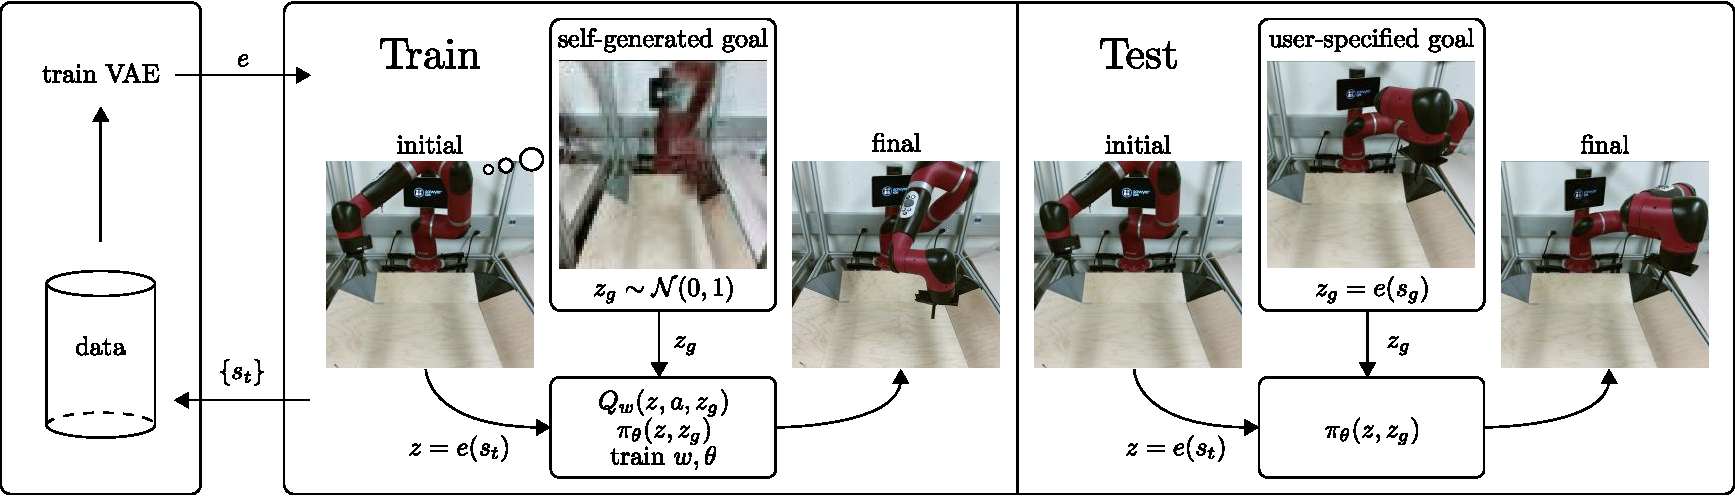
\includegraphics[width=\linewidth]{rig/img/fig1-min-crop.pdf}
    \caption{We train a VAE using data generated by our exploration policy (left). We use the VAE for multiple purposes during training time (middle): to sample goals to train the policy, to embed the observations into a latent space, and to compute distances in the latent space. During test time (right), we embed a specified goal observation $o_g$ into a goal latent $z_g$ as input to the policy.}
    \vspace{-0.1in}
    \label{fig:fig1}
\end{figure}

\section{Related Work}
While prior works on vision-based deep reinforcement learning for robotics can efficiently learn a variety of behaviors such as grasping \citep{pinto2017asymmetric,pinto2015supersizing,levine2017grasping}, pushing \citep{agrawal2016poking,ebert2017videoprediction,finn2016visualforesight}, navigation \citep{pathak2018zeroshot, lange2012autonomous}, and other manipulation tasks \citep{lillicrap2015continuous, levine2016gps, pathak2018zeroshot}, they each make assumptions that limit their applicability to training general-purpose robots.
\citet{levine2016gps} uses time-varying models, which requires an episodic setup that makes them difficult to extend to non-episodic and continual learning scenarios.
\citet{pinto2017asymmetric} proposed a similar approach that uses goal images, but requires instrumented training in simulation. \citet{lillicrap2015continuous} uses fully model-free training, but does not learn goal-conditioned skills. As we show in our experiments, this approach is very difficult to extend to the goal-conditioned setting with image inputs.
Model-based methods that predict images~\citep{watter2015embed,finn2016visualforesight,ebert2017videoprediction,oh2015action} or learn inverse models \citep{agrawal2016poking} can also accommodate various goals, but tend to limit the horizon length due to model drift.
To our knowledge, no prior method uses model-free RL to learn policies conditioned on a single goal image with sufficient efficiency to train directly on real-world robotic systems, without access to ground-truth state or reward information during training.

Our method uses a goal-conditioned value function~\citep{schaul2015uva} in order to solve more general tasks~\citep{sutton2011horde, kaelbling1993goals}. To improve the sample-efficiency of our method during off-policy training, we retroactively relabel samples in the replay buffer with goals sampled from the latent representation.
Goal relabeling has been explored in prior work \citep{kaelbling1993goals,andrychowicz2017her,rauber2017hindsight,levy2017hierarchical,pong2018tdm}. \citet{andrychowicz2017her} and \citet{levy2017hierarchical} use goal relabeling for sparse rewards problems with known goal spaces, restricting the resampled goals to states encountered along that trajectory, since almost any other goal will have no reward signal.
We sample random goals from our learned latent space to use as replay goals for off-policy Q-learning rather than restricting ourselves to states seen along the sampled trajectory, enabling substantially more efficient learning. We use the same goal sampling mechanism for exploration in RL. Goal setting for policy learning has previously been discussed \citep{baranes2012activeimgep} and recently \citet{pere2018unsupervisedgoalspaces} have also proposed using unsupervised learning for setting goals for exploration.
However, we use a model-free Q-learning method that operates on raw state observations and actions, allowing us to solve visually and dynamically complex tasks.

A number of prior works have used unsupervised learning to acquire better representations for RL.
These methods use the learned representation as a substitute for the state for the policy, but require additional information, such as access to the ground truth reward function based on the true state during training time~\citep{higgins2017darla,ha2018world,watter2015embed,finn2016deep,lange2012autonomous,jonschkowski2017pves}, expert trajectories \citep{srinivas2018upn}, human demonstrations \citep{sermanet2017tcn}, or pre-trained object-detection features \citep{lee2017servo}.
In contrast, we learn to generate goals and use the learned representation to obtain a reward function for those goals without any of these extra sources of supervision.
\citet{finn2016deep} combine unsupervised representation learning with reinforcement learning, but in a framework that trains a policy to reach a single goal.
Many prior works have also focused on learning controllable and disentangled representations~\citep{schmidhuber1992learning,chen2016infogan,cheung2014discovering,reed2014learning,desjardins2012disentangling,thomas2017independentlycontrollable}.
We use a method based on variational autoencoders, but these prior techniques are complementary to ours and could be incorporated into our method.

\section{Background}

Our method combines reinforcement learning with goal-conditioned value functions and unsupervised representation learning. Here, we briefly review the techniques that we build on in our method.

\vspace{-0.1in}
\paragraph{Goal-conditioned reinforcement learning.}
In reinforcement learning, the goal is to learn a policy $\pi(s_t) = a_t$ that maximizes expected return, which we denote as 
\mbox{
$R_t = \E[ \sum_{i=t}^T \gamma^{(i - t)} r_i]$
}, 
where $r_i = r(s_i, a_i, s_{i+1})$ and the expectation is under the current policy and environment dynamics.
Here, $s \in \mathcal S$ is a state observation, $a \in \mathcal A$ is an action, and $\gamma$ is a discount factor.
Standard model-free RL learns policies that achieve a single task.
If our aim is instead to obtain a policy that can accomplish a variety of tasks, we can construct a goal-conditioned policy and reward, and optimize the expected return with respect to a goal distribution: $\E_{g \sim G} [\E_{r_i, s_i \sim E, a_i \sim \pi}[R_0]]$, where $\mathcal G$ is the set of goals and the reward is also a function of $g$.
A variety of algorithms can learn goal-conditioned policies, but to enable sample-efficient learning, we focus on algorithms that acquire goal-conditioned Q-functions, which can be trained off-policy.
A goal-conditioned Q-function $Q(s, a, g)$ learns the expected return for the goal $g$ starting from state $s$ and taking action $a$.
Given a state $s$, action $a$, next state $s'$, goal $g$, and correspond reward $r$, one can train an approximate Q-function parameterized by $w$ by minimizing the following Bellman error
\begin{equation}\label{eq:bellman}
   \mathcal E(w) = \frac{1}{2}|| Q_w(s, a, g) - (r +  \gamma \max_{a'} Q_{\bar{w}}(s', a', g))||^2
\end{equation}
where $\bar w$ indicates that $\bar w$ is treated as a constant.
Crucially, one can optimize this loss using off-policy data $(s, a, s', g, r)$ with a standard actor-critic algorithm~\citep{lillicrap2015continuous,fujimoto2018td3,mnih2016asynchronous}.

\vspace{-0.1in}
\paragraph{Variational Autoencoders.}
Variational autoencoders (VAEs) have been demonstrated to learn structured latent representations of high dimensional data~\citep{kingma2014vae}.
The VAE consists of an encoder $p_\phi$, which maps states to latent distributions,
and a decoder $p_\psi$, which maps latents to distributions over states.
The encoder and decoder parameters, $\psi$ and $\phi$ respectively, are jointly trained to maximize
\begin{equation}\label{eq:vae-loss}
    \mathcal L (\psi, \phi; s^{(i)}) = - \beta D_{KL}(q_\phi(z | s^{(i)}) || p(z)) + \mathbb E_{q_\phi(z \mid s^{(i)})} [ \log p_\psi(s^{(i)} \mid z) ],
\end{equation}
where $p(z)$ is some prior, which we take to be the unit Gaussian, $D_{KL}$ is the Kullback-Leibler divergence, and $\beta$ is a hyperparameter that balances the two terms.
The use of $\beta$ values other than one is sometimes referred to as a $\beta$-VAE~\citep{higgins2016beta}.
The encoder $q_\phi$ parameterizes the mean and log-variance diagonal of a Gaussian distribution, $q_\phi(s) = \mathcal N(\mu_\phi(s), \sigma^2_\phi(s))$.
The decoder $p_\psi$ parameterizes a Bernoulli distribution for each pixel value.
This parameterization corresponds to training the decoder with cross-entropy loss on normalized pixel values.
Full details of the hyperparameters are in the Supplementary Material.

\section{Goal-Conditioned Policies with Unsupervised Representation Learning}
To devise a practical algorithm based on goal-conditioned value functions, we must choose a suitable goal representation.
In the absence of domain knowledge and instrumentation, a general-purpose choice is to set the goal space $\mathcal G$ to be the same as the state observations space $\mathcal S$.
This choice is fully general as it can be applied to any task, and still permits considerable user control since the user can choose a ``goal state'' to set a desired goal for a trained goal-conditioned policy.
But when the state space $\mathcal S$ corresponds to high-dimensional sensory inputs
such as images,
\setcounter{footnote}{0}
\footnote{We make the simplifying assumption that the system is Markovian with respect to the sensory input, and one could incorporate memory into the state for partially observed tasks.}
learning a goal-conditioned Q-function and policy becomes exceedingly difficult as we illustrate empirically in Section~\ref{sec:experiments}.

Our method jointly addresses a number of problems that arise when working with high-dimensional inputs such as images:
sample efficient learning, reward specification, and automated goal-setting.
We address these problems by learning a latent embedding using a $\beta$-VAE.
We use this latent space to represent the goal and state and retroactively relabel data with latent goals sampled from the VAE prior to improve sample efficiency.
We also show that distances in the latent space give us a well-shaped reward function for images.
Lastly, we sample from the prior to allow an agent to set and ``practice'' reaching its own goal, removing the need for humans to specify new goals during training time.
We next describe the specific components of our method, and summarize our complete algorithm in Section~\ref{sec:alg_summary}.

\subsection{Sample-Efficient RL with Learned Representations}
One challenging problem with end-to-end approaches for visual RL tasks is that the resulting policy needs to learn both perception and control.
Rather than operating directly on observations, we embed the state $s_t$ and goals $g$ into a latent space $\mathcal Z$ using an encoder $e$ to obtain a latent state $z_t = e(s_t)$ and latent goal $z_g = e(g)$.
To learn a representation of the state and goal space, we train a $\beta$-VAE by executing a random policy and collecting state observations, $\{s^{(i)}\}$, and optimize Equation $\eqref{eq:vae-loss}$.
We then use the mean of the encoder as the state encoding, i.e. $z = e(s) \triangleq \mu_\phi(s)$.

After training the VAE, we train a goal-conditioned Q-function $Q(z, a, z_g)$ and corresponding policy $\pi_\theta(z, z_g)$ in this latent space.
The policy is trained to reach a goal $z_g$ using the reward function discussed in Section \ref{sec:reward-specification}.
For the underlying RL algorithm, we use twin delayed deep deterministic policy gradients (TD3)~\citep{fujimoto2018td3}, though any value-based RL algorithm could be used.
Note that the policy (and Q-function) operates completely in the latent space.
During test time, to reach a specific goal state $g$, we encode the goal $z_g = e(g)$ and input this latent goal to the policy.

As the policy improves, it may visit parts of the state space that the VAE was never trained on, resulting in arbitrary encodings that may not make learning easier.
Therefore, in addition to procedure described above, we fine-tune the VAE using both the randomly generated state observations $\{s^{(i)}\}$ and the state observations collected during exploration.
We show in Section \ref{sec:appendix_online} that this additional training helps the performance of the algorithm.

\subsection{Reward Specification}\label{sec:reward-specification}
Training the goal-conditioned value function requires defining a goal-conditioned reward $r(s,g)$.
Using Euclidean distances in the space of image pixels provides a poor metric, since similar configurations in the world can be extremely different in image space.
In addition to compactly representing high-dimensional observations, we can utilize our representation to obtain a reward function based on a metric that better reflects the similarity between the state and the goal.
One choice for such a reward is to use the negative Mahalanobis distance in the latent space:
% \begin{equation}\label{eq:mahalanobis}
\begin{equation}\nonumber
    r(s, g) = -||e(s) - e(g)||_A = - ||z - z_g||_A,
\end{equation}
where the matrix $A$ weights different dimensions in the latent space.
This approach has an appealing interpretation when we set $A$ to be the precision matrix of the VAE encoder, $q_\phi$.
Since we use a Gaussian encoder, we have that
\begin{equation}\label{eq:reward-log-prob-equivalence}
    r(s, g) = - ||z - z_g||_A \propto \sqrt{\log e_\phi(z_g \mid s)}
\end{equation}
In other words, minimizing this squared distance in the latent space is equivalent to rewarding reaching states that maximize the probability of the latent goal $z_g$.
In practice, we found that setting $A = \mathbf{I}$, corresponding to Euclidean distance, performed better than Mahalanobis distance, though its effect is the same --- to bring $z$ close to $z_g$ and maximize the probability of the latent goal $z_g$ given the observation.
This interpretation would not be possible when using normal autoencoders since distances are not trained to have any probabilistic meaning.
Indeed, we show in Section \ref{sec:experiments} that using distances in a normal autoencoder representation often does not result in meaningful behavior.

\subsection{Improving Sample Efficiency with Latent Goal Relabeling}\label{sec:goal-relabeling}
To further enable sample-efficient learning in the real world, we use the VAE to relabel goals.
Note that we can optimize Equation \eqref{eq:bellman} using any valid $(s, a, s', g, r)$ tuple.
If we could artificially generate these tuples, then we could train our entire RL algorithm without collecting any data.
However, we do not know the system dynamics, and therefore have to sample transitions $(s,a,s')$ by interacting with the world.
However, we have the freedom to relabel the goal and reward synthetically.
In particular, if we have a mechanism for generating goals and computing rewards, then given $(s, a, s')$, we can generate a new goal $g$ and new reward $r(s, a, s', g)$ to produce a new tuple $(s, a, s', g, r)$.
By artificially generating and recomputing rewards, we can convert a single $(s, a, s')$ transition into potentially infinitely many valid training datums.

For image-based tasks, this procedure would require generating goal images, an onerous task on its own.
However, our reinforcement learning algorithm operates directly in the latent space for goals and rewards.
So rather than generating goals $g$, we generate latent goals $z_g$ by sampling from the VAE prior $p(z)$.
We then recompute rewards using Equation~\eqref{eq:reward-log-prob-equivalence}.
By retroactively relabeling the goals and rewards, we obtain much more data to train our value function.
This sampling procedure is made possible by our use of a latent variable model, which is explicitly trained so that sampling from the latent distribution is straightforward.

Retroactively generating goals is also explored in tabular domains by \citet{kaelbling1993goals} and in continuous domains by \citet{andrychowicz2017her} using hindsight experience replay (HER).
However, HER is limited to sampling goals seen along a trajectory, which greatly limits the number and diversity of goals with which one can relabel a given transition.
Our final method uses a mixture of the two strategies: half of the goals are generated from the prior and half from goals seen along the trajectory.
We show in Section \ref{sec:experiments} that relabeling the goal with samples from the VAE prior results in significantly better sample-efficiency.

% \vspace{-0.1in}
\begin{algorithm}
   	\footnotesize
   	\caption{RIG: Reinforcement learning with imagined goals}
    % \vspace{-0.2in}
   	\label{alg:tbd}
   	\begin{multicols}{2}
   	\begin{algorithmic}[1]
    \REQUIRE VAE encoder $q_\phi$, VAE decoder $p_\psi$, policy $\pi_\theta$, goal-conditioned value function $Q_w$.
    \STATE Collect $\mathcal D = \{s^{(i)}\}$ using exploration policy.
    \STATE Train $\beta$-VAE on $\mathcal D$ by optimizing \eqref{eq:vae-loss}.
    \FOR{$n=0,...,N-1$ episodes}
        \STATE Sample latent goal from prior $z_g \sim p(z)$.
        \STATE Sample initial state $s_0 \sim E$.
        \FOR{$t=0,...,H -1$ steps}
            \STATE Get action $a_t = \pi_\theta(e(s_t), z_g) + \text{noise}$.
            \STATE Get next state $s_{t+1} \sim p(\cdot \mid s_t, a_t)$.
            \STATE Store $(s_t, a_t, s_{t+1}, z_g)$ into replay buffer $\mathcal R$.
            \STATE Sample transition $(s, a, s', z_g) \sim \mathcal R$.
            \STATE Encode $z' = e(s')$.
            \STATE (Probability $0.5$) replace $z_g$ with $z_g' \sim p(z)$.
            \STATE Compute new reward $r = -||z' - z_g||$.
            \STATE Minimize \eqref{eq:bellman} using $(z, a, z', z_g, r)$.
        \ENDFOR
        \STATE Fine-tune $\beta$-VAE every $K$ episodes on mixture of $\mathcal D$ and $\mathcal R$.
    \ENDFOR
   	\end{algorithmic}
   	\end{multicols}
   	\vspace{-0.15in}
\end{algorithm}

\subsection{Automated Goal-Generation for Exploration}
If we do not know which particular goals will be provided at test time, we would like our RL agent to carry out a self-supervised ``practice'' phase during training, where the algorithm proposes its own goals, and then practices how to reach them.
Since the VAE prior represents a distribution over latent goals and state observations, we again sample from this distribution to obtain plausible goals.
After sampling a goal latent from the prior $z_g \sim p(z)$, we give this to our policy $\pi(z, z_g)$ to collect data.

\subsection{Algorithm Summary}
\label{sec:alg_summary}

We call the complete algorithm reinforcement learning with imagined goals (RIG) and summarize it in Algorithm \ref{alg:tbd}.
We first collect data with a simple exploration policy, though any exploration strategy could be used for this stage, including off-the-shelf exploration bonuses~\citep{pathak2017curiosity, bellemare2016unifying} or unsupervised reinforcement learning methods~\citep{eysenbach2018diayn, florensa2017stochastic}.
Then, we train a VAE latent variable model on state observations and finetune it over the course of training.
We use this latent variable model for multiple purposes:
We sample a latent goal $z_g$ from the model and condition the policy on this goal.
We embed all states and goals using the model's encoder.
When we train our goal-conditioned value function, we resample goals from the prior and compute rewards in the latent space using Equation \eqref{eq:reward-log-prob-equivalence}.
Any RL algorithm that trains Q-functions could be used, and we use TD3~\citep{fujimoto2018td3} in our implementation.

\begin{figure}
    \centering
    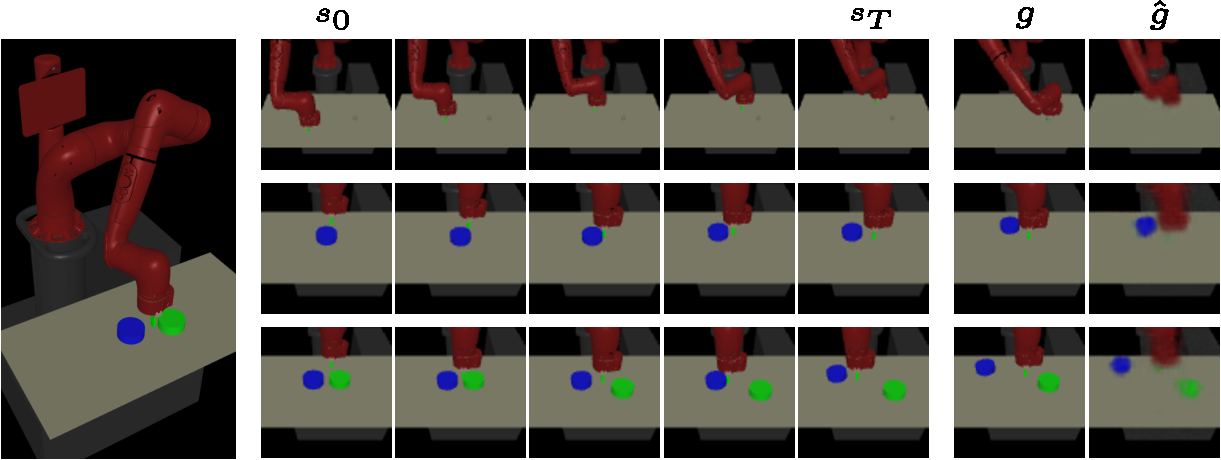
\includegraphics[width=0.99\linewidth]{rig/img/nips18_fig_rollouts-crop.pdf}
    % \vspace{-0.1in}
    \caption{(Left) The simulated environment. (Right) Test rollouts from our learned policy on the three simulated environments. Each row is one rollout. The middle shows the goal image $g$ and its VAE reconstruction $\hat g$. The right columns shows frames from the trajectory to reach the given goal.}
    \vspace{-0.1in}
    \label{fig:sim_screenshot}
\end{figure}

\section{Experiments}\label{sec:experiments}
Our experiments address the following questions:
\begin{enumerate}
    \item How does our method compare to prior model-free RL algorithms in terms of sample efficiency and performance, when learning continuous control tasks from images?
    \item How critical is each component of our algorithm for efficient learning?
    \item Does our method work on tasks where the state space cannot be easily specified ahead of time, such as tasks that require interaction with variable numbers of objects?
    \item Can our method scale to real world vision-based robotic control tasks?
\end{enumerate}
For the first two questions, we evaluate our method against a number of prior algorithms and ablated versions of our approach on a suite of simulated and real-world tasks:
\textit{Visual Reacher}: a MuJoCo~\citep{todorov12mujoco} environment with a 7-dof Sawyer arm reaching goal positions.
The arm is shown the left of Figure \ref{fig:sim_screenshot}.
The end-effector (EE) is constrained to a 2-dimensional rectangle parallel to a table.
The action controls EE velocity within a maximum velocity.
\textit{Visual Pusher}: a MuJoCo environment with a 7-dof Sawyer arm and a small puck on a table that the arm must push to a target push.
\textit{Visual Multi-Object Pusher}: a copy of the Visual Pusher environment with two pucks.
Detailed descriptions of the environments are provided in the Supplementary Material.

Solving these tasks directly from images poses a challenge since the controller must learn both perception and control.
The evaluation metric is the distance of objects (including the arm) to their respective goals.
To evaluate our policy, we set the environment to a sampled goal position, capture an image, and encode the image to use as the goal.
Although we use the ground-truth positions for evaluation, \textbf{we do not use the ground-truth positions for training the policies}.
The only inputs from the environment that our algorithm receives are the image observations.
For Visual Reacher, we pretrained the VAE with 100 images.
For other tasks, we used 10,000 images.

\begin{figure}
    \centering
    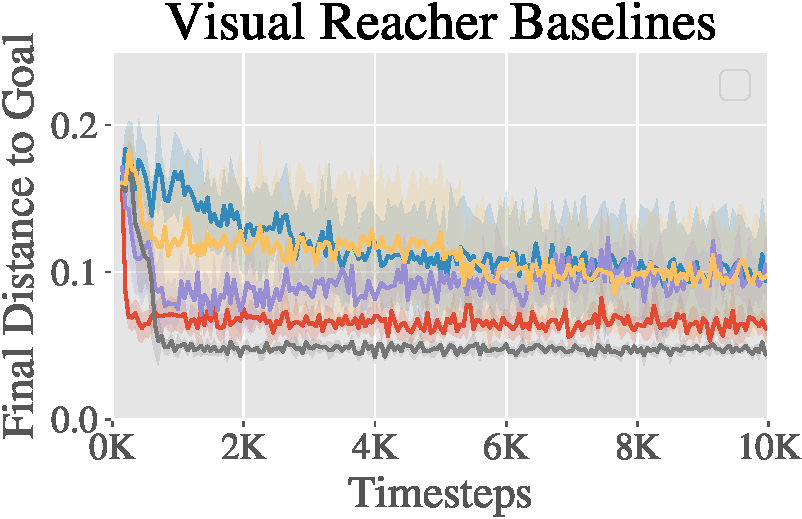
\includegraphics[height=0.19\linewidth]{rig/img/reacher_baselines_legend_right.pdf}
    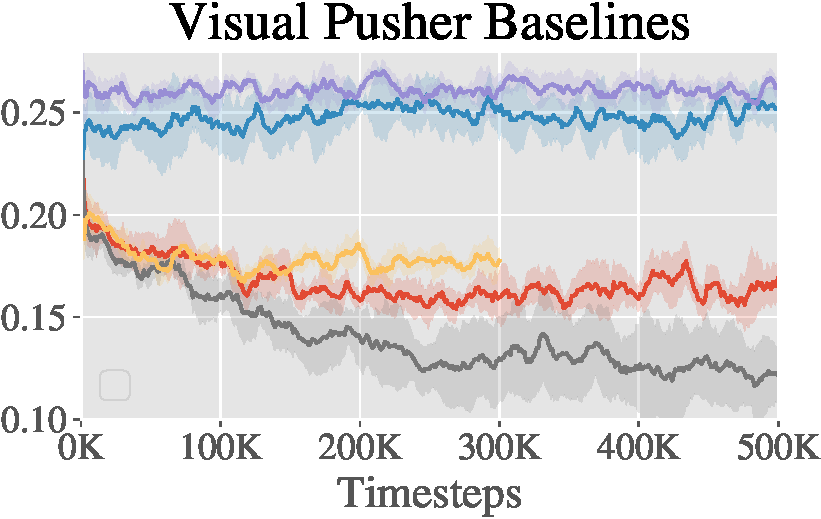
\includegraphics[height=0.19\linewidth]{rig/img/pusher_baselines}
    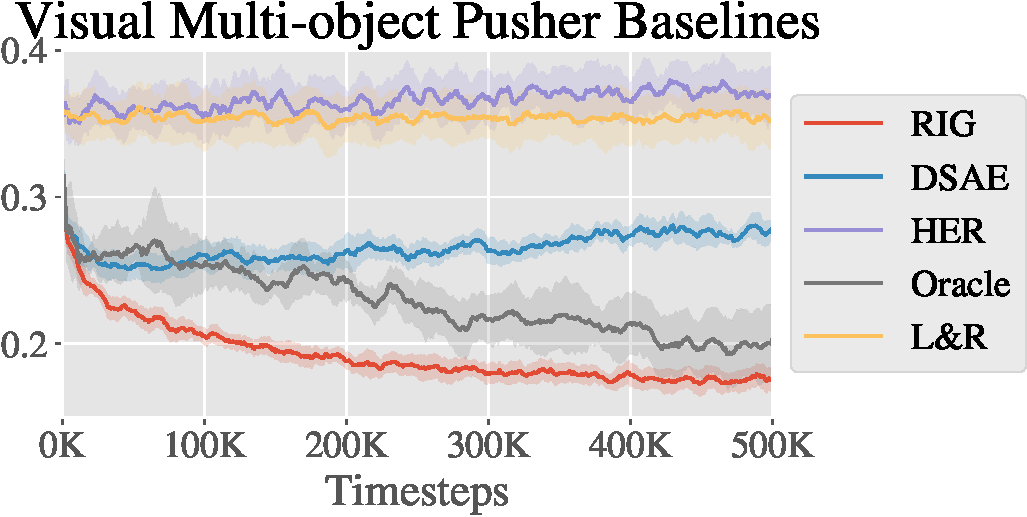
\includegraphics[height=0.19\linewidth]{rig/img/multiobj_pusher_baselines.pdf}
    \vspace{-0.1in}
    \caption{Simulation results, final distance to goal vs simulation steps\protect\footnotemark. 
    RIG (red) consistently outperforms the baselines, except for the oracle which uses ground truth object state for observations and rewards. On the hardest task, only our method and the oracle discover viable solutions.}
    \vspace{-0.2in}
    \label{fig:sim_results}
\end{figure}

\footnotetext{In all our simulation results, each plot shows a 95\% confidence interval of the mean across 5 seeds.}

\sloppy We compare our method with the following prior works.
\textit{L\&R}: Lange and Riedmiller~\citep{lange2010deep} trains an autoencoder to handle images.
\textit{DSAE}: Deep spatial autoencoders~\citep{finn2016deep} learns a spatial autoencoder and uses guided policy search~\citep{levine2016gps} to achieve a single goal image.
\textit{HER}: Hindsight experience replay~\citep{andrychowicz2017her} utilizes a sparse reward signal and relabeling trajectories with achieved goals.
\textit{Oracle}: RL with direct access to state information for observations and rewards.

To our knowledge, no prior work demonstrates policies that can reach a variety of goal images without access to a true-state reward function, and so we needed to make modifications to make the comparisons feasible.
L\&R assumes a reward function from the environment.
Since we have no state-based reward function, we specify the reward function as distance in the autoencoder latent space.
HER does not embed inputs into a latent space but instead operates directly on the input, so we use pixel-wise mean squared error (MSE) as the metric.
DSAE is trained only for a single goal, so we allow the method to generalize to a variety of test goal images by using a goal-conditioned Q-function.
To make the implementations comparable, we use the same off-policy algorithm to train L\&R, HER, and our method (TD3~\citep{fujimoto2018td3}).
Unlike our method, prior methods do not specify how to select goals during training, so we favorably give them real images as goals for rollouts, sampled from the same distribution that we use to test.

We see in Figure \ref{fig:sim_results} that our method can efficiently learn policies from visual inputs to perform simulated reaching and pushing, without access to the object state.
Our approach substantially outperforms the prior methods, for which the use of image goals and observations poses a major challenge.
HER struggles because pixel-wise MSE is hard to optimize. Our latent-space rewards are much better shaped and allow us to learn more complex tasks.
Finally, our method is close to the state-based ``oracle" method in terms of sample efficiency and performance, without having any access to object state.
Notably, in the multi-object environment, our method actually outperforms the oracle, likely because the state-based reward contains local minima.
Overall, these result show that our method is capable of handling raw image observations much more effectively than previously proposed goal-conditioned RL methods. Next, we perform ablations to evaluate our contributions in isolation. Results on Visual Pusher are shown but see the Supplementary Material (section \ref{sec:appendix}) for experiments on all three simulated environments.

\paragraph{Reward Specification Comparison}

\begin{wrapfigure}{r}{6cm}
    \centering
    \vspace{-0.2in}
    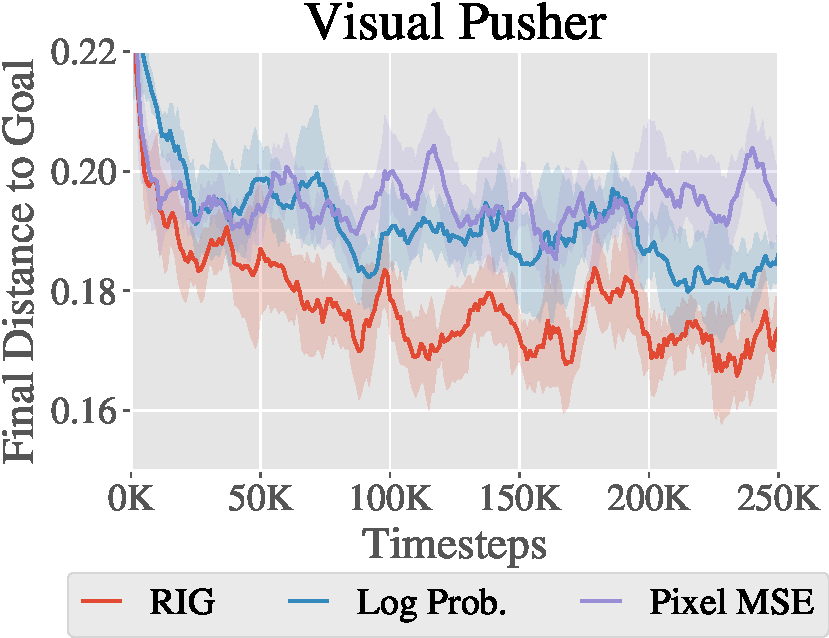
\includegraphics[width=\linewidth]{rig/img/pusher_reward_type_ablation_main.pdf}
    \vspace{-0.2in}
    \captionsetup{format=plain, justification=justified}
    \caption{Reward type ablation results. RIG (red), which uses latent Euclidean distance, outperforms the other methods.}
    \vspace{-0.1in}
    \label{fig:reward-ablation}
\end{wrapfigure}
We evaluate how effective distances in the VAE latent space are for the Visual Pusher task.
We keep our method the same, and only change the reward function that we use to train the goal-conditioned valued function.
We include the following methods for comparison:
\textit{Latent Distance}, which is the reward used in RIG, i.e. $A = \mathbf{I}$ in Equation \eqref{eq:reward-log-prob-equivalence};
\textit{Log Probability}, which uses the Mahalanobis distance in Equation \eqref{eq:reward-log-prob-equivalence}, where $A$ is the precision matrix of the encoder;
and \textit{Pixel MSE}, which computes mean-squared error (MSE) between state and goal in pixel space.
\footnote{To compute the pixel MSE for a sampled latent goal, we decode the goal latent using the VAE decoder, $p_\psi$, to generate the corresponding goal image.}
In Figure \ref{fig:reward-ablation}, we see that latent distance significantly outperforms the log probability.
We suspect that small variances of the VAE encoder results in drastically large rewards, making the learning more difficult.
We also see that latent distances results in faster learning when compared to pixel MSE.

\newpage

\paragraph{Relabeling Strategy Comparison}

\begin{wrapfigure}{r}{6cm}
    \centering
    \vspace{-0.2in}
    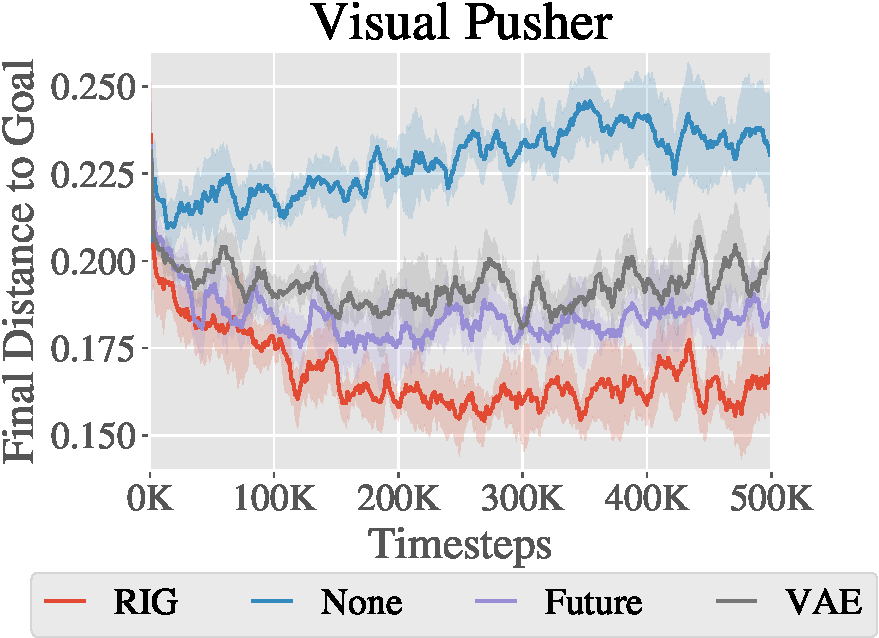
\includegraphics[width=\linewidth]{rig/img/pusher_relabeling_ablation_main.pdf}
    \vspace{-0.15in}
    \captionsetup{format=plain, justification=justified}
    \caption{Relabeling ablation results. RIG (red), which uses a mixture of VAE and HER, outperforms the other methods.}
    \vspace{-0.2in}
    \label{fig:relabel-ablation}
\end{wrapfigure}

As described in section \ref{sec:goal-relabeling}, our method uses a novel goal relabeling method based on sampling from the generative model.
To isolate how much our new goal relabeling method contributes to our algorithm, we vary the resampling strategy while fixing other components of our algorithm.
The resampling strategies that we consider are:
\textit{Future}, relabeling the goal for a transition by sampling uniformly from future states in the trajectory as done in \citet{andrychowicz2017her};
\textit{VAE}, sampling goals from the VAE only;
\textit{RIG}, relabeling goals with probability $0.5$ from the VAE and probability $0.5$ using the future strategy;
and \textit{None}, no relabeling.
In Figure \ref{fig:relabel-ablation}, we see that sampling from the VAE and Future is significantly better than not relabeling at all. In RIG, we use an equal mixture of the VAE and Future sampling strategies, which performs best by a large margin. Appendix section \ref{sec:appendix_relabeling_ablation} contains results on all simulated environments, and section \ref{sec:her_relabeling_ablation} considers relabeling strategies with a known goal distribution.

\begin{wrapfigure}{r}{6cm}
    \centering
    \vspace{-0.2in}
    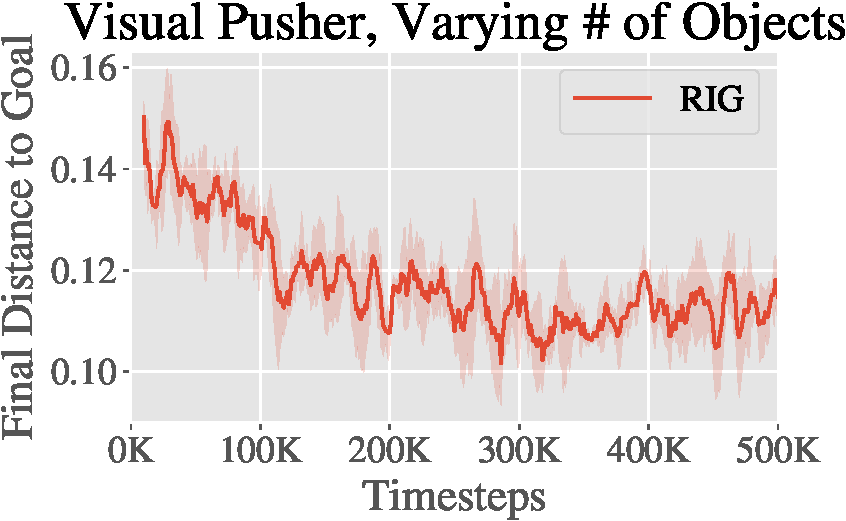
\includegraphics[width=\linewidth]{rig/img/pusher_vary_multiobject.pdf}
    \vspace{-0.1in}
    \captionsetup{format=plain, justification=justified}
    \caption{Training curve for learning with varying number of objects.}
    \vspace{-0.15in}
    \label{fig:multiobject}
\end{wrapfigure}

\vspace{-0.1in}
\paragraph{Learning with Variable Numbers of Objects}
A major advantage of working directly from pixels is that the policy input can easily represent combinatorial structure in the environment, which would be difficult to encode into a fixed-length state vector even if a perfect perception system were available.
For example, if a robot has to interact with different combinations and numbers of objects, picking a single MDP state representation would be challenging, even with access to object poses.
By directly processing images for both the state and the goal, no modification is needed to handle the combinatorial structure: the number of pixels always remains the same, regardless of how many objects are in the scene.

We demonstrate that our method can handle this difficult scenario by evaluating on a task where the environment, based on the Visual Multi-Object Pusher, randomly contains zero, one, or two objects in each episode during testing.
During training, each episode still always starts with both objects in the scene, so the experiments tests whether a trained policy can handle variable numbers of objects at test time.
Figure \ref{fig:multiobject} shows that our method can learn to solve this task successfully, without decrease in performance from the base setting where both objects are present (in Figure~\ref{fig:sim_results}).
Developing and demonstrating algorithms that solve tasks with varied underlying structure is an important step toward creating autonomous agents that can handle the diversity of tasks present ``in the wild.''

\begin{figure}[ht!]
    \centering
    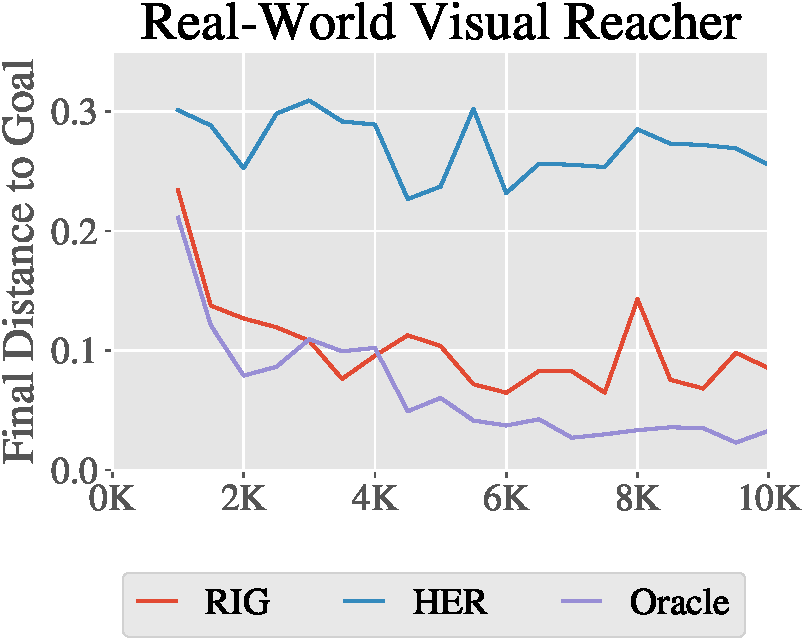
\includegraphics[width=0.31\linewidth]{rig/img/real_reacher.pdf}
    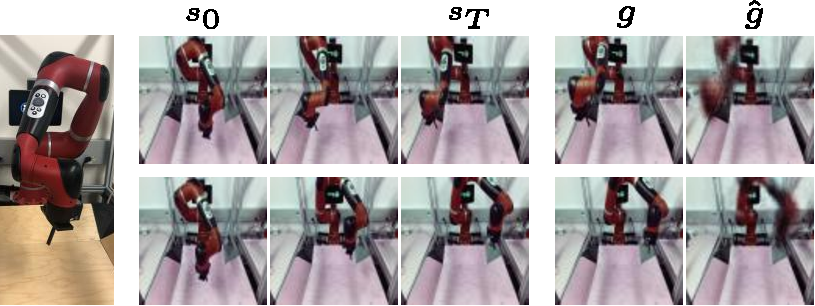
\includegraphics[width=0.67\linewidth]{rig/img/real_rollouts-crop.pdf}
    \caption{(Left) Our method compared to the HER baseline and oracle on a real-world visual reaching task. (Middle) Our robot setup is pictured. (Right) Test rollouts of our learned policy. }
    %\vspace{-0.2in}
    \label{fig:realworld-robot-results}
\end{figure}

\begin{figure}[ht!]
    \centering
    \begin{subfigure}[b]{0.28\textwidth}
        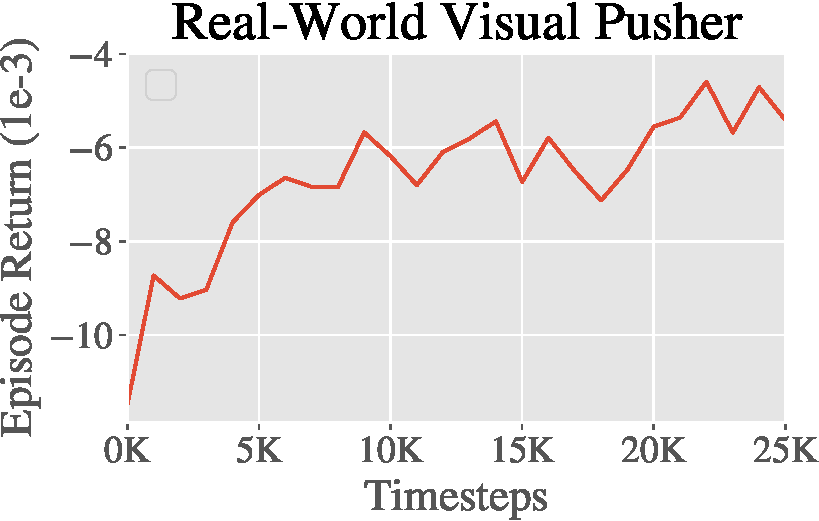
\includegraphics[width=1\linewidth]{rig/img/pusher_learning_curve-crop.pdf}
    \end{subfigure}
    \begin{subfigure}[b]{0.4\textwidth}
        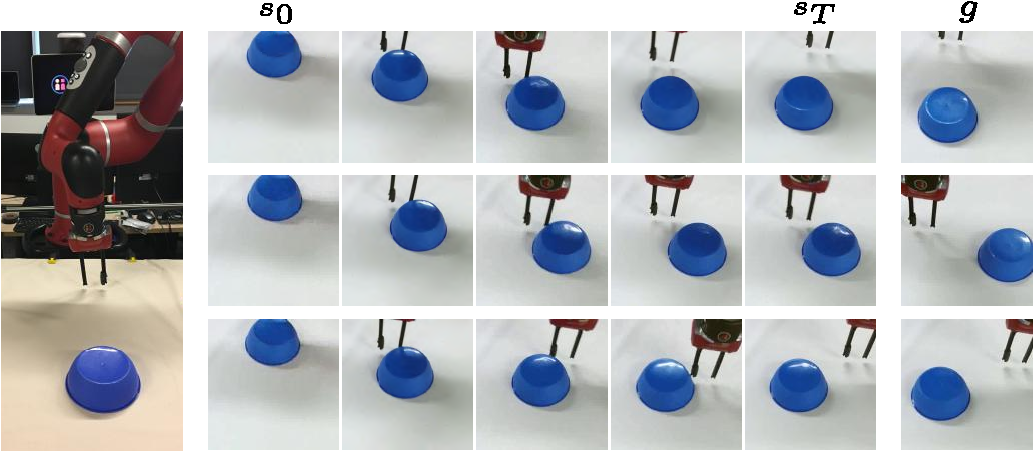
\includegraphics[width=1\linewidth]{rig/img/real_pusher_rollouts.pdf}
    \end{subfigure}
    \begin{subfigure}[b]{0.3\textwidth}
    %\vspace{-1cm}
        \begin{flushright}
            \small{Puck Distance to Goal (cm)} \\
            \vspace{0cm}           
            {\renewcommand{\arraystretch}{1.2}%
            \begin{tabular}{  c | c }
             \hline
               $\quad\,$ RIG $\quad \,$ & $\quad\,$ HER $\quad\,$ \\ \hline
                $\mathbf{4.5 \pm 2.5}$ & $14.9 \pm 5.4$  \\
            \end{tabular}
            }
        \end{flushright}
        \vspace{0.1cm}
    \end{subfigure}
    \caption{(Left) The learning curve for real-world pushing. (Middle) Our robot pushing setup is pictured, with frames from test rollouts of our learned policy. (Right) Our method compared to the HER baseline on the real-world visual pushing task. We evaluated the performance of each method by manually measuring the distance between the goal position of the puck and final position of the puck for 15 test rollouts, reporting mean and standard deviation.}
    \vspace{-0.2in}
    \label{fig:realworld-robot-pushing-results}
\end{figure}

\subsection{Visual RL with Physical Robots}
RIG is a practical and straightforward algorithm to apply to real physical systems:
the efficiency of off-policy learning with goal relabeling makes training times manageable, while the use of image-based rewards through the learned representation frees us from the burden of manually design reward functions, which itself can require hand-engineered perception systems~\citep{rusu2016sim}.
We trained policies for visual reaching and pushing on a real-world Sawyer robotic arm, shown in Figure \ref{fig:realworld-robot-results}.
The control setup matches Visual Reacher and Visual Pusher respectively, meaning that \textbf{the only input from the environment consists of camera images}.

We see in Figure \ref{fig:realworld-robot-results} that our method is applicable to real-world robotic tasks, almost matching the state-based oracle method and far exceeding the baseline method on the reaching task. Our method needs just 10,000 samples or about an hour of real-world interaction time to solve visual reaching.

Real-world pushing results are shown in Figure \ref{fig:realworld-robot-pushing-results}. To solve visual pusher, which is more visually complicated and requires reasoning about the contact between the arm and object, our method requires about 25,000 samples, which is still a reasonable amount of real-world training time. Note that unlike previous results, we do not have access to the true puck position during training so for the learning curve we report test episode returns on the VAE latent distance reward. We see RIG making steady progress at optimizing the latent distance as learning proceeds.

\section{Discussion and Future Work}

In this paper, we present a new RL algorithm that can efficiently solve goal-conditioned, vision-based tasks without access to any ground truth state or reward functions.
Our method trains a generative model that is used for multiple purposes: we embed the state and goals using the encoder; we sample from the prior to generate goals for exploration; we also sample latents to retroactively relabel goals and rewards; and we use distances in the latent space for rewards to train a goal-conditioned value function.
We show that these components culminate in a sample efficient algorithm that works directly from vision.
As a result, we are able to apply our method to a variety of simulated visual tasks, including a variable-object task that cannot be easily represented with a fixed length vector, as well as real world robotic tasks.
Algorithms that can learn in the real world and directly use raw images can allow a single policy to solve a large and diverse set of tasks, even when these tasks require distinct internal representations.

The method we presented can be extended in a number of ways.
First, an exciting line of future work would be to combine our method with existing work on exploration and intrinsic motivation.
In particular, our method already provides a natural mechanism for autonomously generating goals by sampling from the prior.
Modifying this procedure to not only be goal-oriented but also, e.g., be information seeking or uncertainty aware could provide better and safer exploration.
Second, since our method operates directly from images, a single policy could potentially solve a large diverse set of visual tasks, even if those tasks have different underlying state representations.
Combining these ideas with methods from multitask learning and meta-learning is a promising path to creating general-purpose agents that can continuously and efficiently acquire skills.
Lastly, while RIG uses goal images, extending the method to allow goals specified by demonstrations or more abstract representations such as language would enable our system to be much more flexible in interfacing with humans and therefore more practical.


\chapter{SkewFit: State-Covering Self-Supervised Reinforcement Learning}\label{chapter:skewfit}
%  % \documentclass{article} % For LaTeX2e
% % if you need to pass options to natbib, use, e.g.:
% %\PassOptionsToPackage{numbers, compress}{natbib}

% \usepackage[utf8]{inputenc} % allow utf-8 input
% \usepackage[T1]{fontenc}    % use 8-bit T1 fonts
% \usepackage{hyperref}       % hyperlinks
% \usepackage{url}            % simple URL typesetting
% \usepackage{booktabs}       % professional-quality tables
% \usepackage{amsfonts}       % blackboard math symbols
% \usepackage{nicefrac}       % compact symbols for 1/2, etc.
% \usepackage{microtype}      % microtypography
% \usepackage{graphicx}
% \usepackage{subcaption}

% % hyperref makes hyperlinks in the resulting PDF.
% % If your build breaks (sometimes temporarily if a hyperlink spans a page)
% % please comment out the following usepackage line and replace
% % \usepackage{icml2020} with \usepackage[nohyperref]{icml2020} above.
% \usepackage{hyperref}

% % Attempt to make hyperref and algorithmic work together better:
% \newcommand{\theHalgorithm}{\arabic{algorithm}}


% % Use the following line for the initial blind version submitted for review:
% % \usepackage{icml2020}

% % If accepted, instead use the following line for the camera-ready submission:
% \usepackage[accepted]{icml2020}

% \icmltitlerunning{\METHOD: State-Covering Self-Supervised Reinforcement Learning}

% %%%%% NEW MATH DEFINITIONS %%%%%

\usepackage{amsmath,amsfonts,bm}
\usepackage{mathtools}

% Mark sections of captions for referring to divisions of figures
\newcommand{\figleft}{{\em (Left)}}
\newcommand{\figcenter}{{\em (Center)}}
\newcommand{\figright}{{\em (Right)}}
\newcommand{\figtop}{{\em (Top)}}
\newcommand{\figbottom}{{\em (Bottom)}}
\newcommand{\captiona}{{\em (a)}}
\newcommand{\captionb}{{\em (b)}}
\newcommand{\captionc}{{\em (c)}}
\newcommand{\captiond}{{\em (d)}}

% Highlight a newly defined term
\newcommand{\newterm}[1]{{\bf #1}}


% Figure reference, lower-case.
\def\figref#1{figure~\ref{#1}}
% Figure reference, capital. For start of sentence
\def\Figref#1{Figure~\ref{#1}}
\def\twofigref#1#2{figures \ref{#1} and \ref{#2}}
\def\quadfigref#1#2#3#4{figures \ref{#1}, \ref{#2}, \ref{#3} and \ref{#4}}
% Section reference, lower-case.
\def\secref#1{section~\ref{#1}}
% Section reference, capital.
\def\Secref#1{Section~\ref{#1}}
% Reference to two sections.
\def\twosecrefs#1#2{sections \ref{#1} and \ref{#2}}
% Reference to three sections.
\def\secrefs#1#2#3{sections \ref{#1}, \ref{#2} and \ref{#3}}
% Reference to an equation, lower-case.
\def\eqref#1{equation~\ref{#1}}
% Reference to an equation, upper case
\def\Eqref#1{Equation~\ref{#1}}
% A raw reference to an equation---avoid using if possible
\def\plaineqref#1{\ref{#1}}
% Reference to a chapter, lower-case.
\def\chapref#1{chapter~\ref{#1}}
% Reference to an equation, upper case.
\def\Chapref#1{Chapter~\ref{#1}}
% Reference to a range of chapters
\def\rangechapref#1#2{chapters\ref{#1}--\ref{#2}}
% Reference to an algorithm, lower-case.
\def\algref#1{algorithm~\ref{#1}}
% Reference to an algorithm, upper case.
\def\Algref#1{Algorithm~\ref{#1}}
\def\twoalgref#1#2{algorithms \ref{#1} and \ref{#2}}
\def\Twoalgref#1#2{Algorithms \ref{#1} and \ref{#2}}
% Reference to a part, lower case
\def\partref#1{part~\ref{#1}}
% Reference to a part, upper case
\def\Partref#1{Part~\ref{#1}}
\def\twopartref#1#2{parts \ref{#1} and \ref{#2}}

\def\ceil#1{\lceil #1 \rceil}
\def\floor#1{\lfloor #1 \rfloor}
\def\1{\bm{1}}
\newcommand{\train}{\mathcal{D}}
\newcommand{\valid}{\mathcal{D_{\mathrm{valid}}}}
\newcommand{\test}{\mathcal{D_{\mathrm{test}}}}

\def\eps{{\epsilon}}


% Random variables
\def\reta{{\textnormal{$\eta$}}}
\def\ra{{\textnormal{a}}}
\def\rb{{\textnormal{b}}}
\def\rc{{\textnormal{c}}}
\def\rd{{\textnormal{d}}}
\def\re{{\textnormal{e}}}
\def\rf{{\textnormal{f}}}
\def\rg{{\textnormal{g}}}
\def\rh{{\textnormal{h}}}
\def\ri{{\textnormal{i}}}
\def\rj{{\textnormal{j}}}
\def\rk{{\textnormal{k}}}
\def\rl{{\textnormal{l}}}
% rm is already a command, just don't name any random variables m
\def\rn{{\textnormal{n}}}
\def\ro{{\textnormal{o}}}
\def\rp{{\textnormal{p}}}
\def\rq{{\textnormal{q}}}
\def\rr{{\textnormal{r}}}
\def\rs{{\textnormal{s}}}
\def\rt{{\textnormal{t}}}
\def\ru{{\textnormal{u}}}
\def\rv{{\textnormal{v}}}
\def\rw{{\textnormal{w}}}
\def\rx{{\textnormal{x}}}
\def\ry{{\textnormal{y}}}
\def\rz{{\textnormal{z}}}

% Random vectors
\def\rvepsilon{{\mathbf{\epsilon}}}
\def\rvtheta{{\mathbf{\theta}}}
\def\rva{{\mathbf{a}}}
\def\rvb{{\mathbf{b}}}
\def\rvc{{\mathbf{c}}}
\def\rvd{{\mathbf{d}}}
\def\rve{{\mathbf{e}}}
\def\rvf{{\mathbf{f}}}
\def\rvg{{\mathbf{g}}}
\def\rvh{{\mathbf{h}}}
\def\rvu{{\mathbf{i}}}
\def\rvj{{\mathbf{j}}}
\def\rvk{{\mathbf{k}}}
\def\rvl{{\mathbf{l}}}
\def\rvm{{\mathbf{m}}}
\def\rvn{{\mathbf{n}}}
\def\rvo{{\mathbf{o}}}
\def\rvp{{\mathbf{p}}}
\def\rvq{{\mathbf{q}}}
\def\rvr{{\mathbf{r}}}
\def\rvs{{\mathbf{s}}}
\def\rvt{{\mathbf{t}}}
\def\rvu{{\mathbf{u}}}
\def\rvv{{\mathbf{v}}}
\def\rvw{{\mathbf{w}}}
\def\rvx{{\mathbf{x}}}
\def\rvy{{\mathbf{y}}}
\def\rvz{{\mathbf{z}}}

% Elements of random vectors
\def\erva{{\textnormal{a}}}
\def\ervb{{\textnormal{b}}}
\def\ervc{{\textnormal{c}}}
\def\ervd{{\textnormal{d}}}
\def\erve{{\textnormal{e}}}
\def\ervf{{\textnormal{f}}}
\def\ervg{{\textnormal{g}}}
\def\ervh{{\textnormal{h}}}
\def\ervi{{\textnormal{i}}}
\def\ervj{{\textnormal{j}}}
\def\ervk{{\textnormal{k}}}
\def\ervl{{\textnormal{l}}}
\def\ervm{{\textnormal{m}}}
\def\ervn{{\textnormal{n}}}
\def\ervo{{\textnormal{o}}}
\def\ervp{{\textnormal{p}}}
\def\ervq{{\textnormal{q}}}
\def\ervr{{\textnormal{r}}}
\def\ervs{{\textnormal{s}}}
\def\ervt{{\textnormal{t}}}
\def\ervu{{\textnormal{u}}}
\def\ervv{{\textnormal{v}}}
\def\ervw{{\textnormal{w}}}
\def\ervx{{\textnormal{x}}}
\def\ervy{{\textnormal{y}}}
\def\ervz{{\textnormal{z}}}

% Random matrices
\def\rmA{{\mathbf{A}}}
\def\rmB{{\mathbf{B}}}
\def\rmC{{\mathbf{C}}}
\def\rmD{{\mathbf{D}}}
\def\rmE{{\mathbf{E}}}
\def\rmF{{\mathbf{F}}}
\def\rmG{{\mathbf{G}}}
\def\rmH{{\mathbf{H}}}
\def\rmI{{\mathbf{I}}}
\def\rmJ{{\mathbf{J}}}
\def\rmK{{\mathbf{K}}}
\def\rmL{{\mathbf{L}}}
\def\rmM{{\mathbf{M}}}
\def\rmN{{\mathbf{N}}}
\def\rmO{{\mathbf{O}}}
\def\rmP{{\mathbf{P}}}
\def\rmQ{{\mathbf{Q}}}
\def\rmR{{\mathbf{R}}}
\def\rmS{{\mathbf{S}}}
\def\rmT{{\mathbf{T}}}
\def\rmU{{\mathbf{U}}}
\def\rmV{{\mathbf{V}}}
\def\rmW{{\mathbf{W}}}
\def\rmX{{\mathbf{X}}}
\def\rmY{{\mathbf{Y}}}
\def\rmZ{{\mathbf{Z}}}

% Elements of random matrices
\def\ermA{{\textnormal{A}}}
\def\ermB{{\textnormal{B}}}
\def\ermC{{\textnormal{C}}}
\def\ermD{{\textnormal{D}}}
\def\ermE{{\textnormal{E}}}
\def\ermF{{\textnormal{F}}}
\def\ermG{{\textnormal{G}}}
\def\ermH{{\textnormal{H}}}
\def\ermI{{\textnormal{I}}}
\def\ermJ{{\textnormal{J}}}
\def\ermK{{\textnormal{K}}}
\def\ermL{{\textnormal{L}}}
\def\ermM{{\textnormal{M}}}
\def\ermN{{\textnormal{N}}}
\def\ermO{{\textnormal{O}}}
\def\ermP{{\textnormal{P}}}
\def\ermQ{{\textnormal{Q}}}
\def\ermR{{\textnormal{R}}}
\def\ermS{{\textnormal{S}}}
\def\ermT{{\textnormal{T}}}
\def\ermU{{\textnormal{U}}}
\def\ermV{{\textnormal{V}}}
\def\ermW{{\textnormal{W}}}
\def\ermX{{\textnormal{X}}}
\def\ermY{{\textnormal{Y}}}
\def\ermZ{{\textnormal{Z}}}

% Vectors
\def\vzero{{\bm{0}}}
\def\vone{{\bm{1}}}
\def\vmu{{\bm{\mu}}}
\def\vtheta{{\bm{\theta}}}
\def\va{{\bm{a}}}
\def\vb{{\bm{b}}}
\def\vc{{\bm{c}}}
\def\vd{{\bm{d}}}
\def\ve{{\bm{e}}}
\def\vf{{\bm{f}}}
\def\vg{{\bm{g}}}
\def\vh{{\bm{h}}}
\def\vi{{\bm{i}}}
\def\vj{{\bm{j}}}
\def\vk{{\bm{k}}}
\def\vl{{\bm{l}}}
\def\vm{{\bm{m}}}
\def\vn{{\bm{n}}}
\def\vo{{\bm{o}}}
\def\vp{{\bm{p}}}
\def\vq{{\bm{q}}}
\def\vr{{\bm{r}}}
\def\vs{{\bm{s}}}
\def\vt{{\bm{t}}}
\def\vu{{\bm{u}}}
\def\vv{{\bm{v}}}
\def\vw{{\bm{w}}}
\def\vx{{\bm{x}}}
\def\vy{{\bm{y}}}
\def\vz{{\bm{z}}}

% Elements of vectors
\def\evalpha{{\alpha}}
\def\evbeta{{\beta}}
\def\evepsilon{{\epsilon}}
\def\evlambda{{\lambda}}
\def\evomega{{\omega}}
\def\evmu{{\mu}}
\def\evpsi{{\psi}}
\def\evsigma{{\sigma}}
\def\evtheta{{\theta}}
\def\eva{{a}}
\def\evb{{b}}
\def\evc{{c}}
\def\evd{{d}}
\def\eve{{e}}
\def\evf{{f}}
\def\evg{{g}}
\def\evh{{h}}
\def\evi{{i}}
\def\evj{{j}}
\def\evk{{k}}
\def\evl{{l}}
\def\evm{{m}}
\def\evn{{n}}
\def\evo{{o}}
\def\evp{{p}}
\def\evq{{q}}
\def\evr{{r}}
\def\evs{{s}}
\def\evt{{t}}
\def\evu{{u}}
\def\evv{{v}}
\def\evw{{w}}
\def\evx{{x}}
\def\evy{{y}}
\def\evz{{z}}

% Matrix
\def\mA{{\bm{A}}}
\def\mB{{\bm{B}}}
\def\mC{{\bm{C}}}
\def\mD{{\bm{D}}}
\def\mE{{\bm{E}}}
\def\mF{{\bm{F}}}
\def\mG{{\bm{G}}}
\def\mH{{\bm{H}}}
\def\mI{{\bm{I}}}
\def\mJ{{\bm{J}}}
\def\mK{{\bm{K}}}
\def\mL{{\bm{L}}}
\def\mM{{\bm{M}}}
\def\mN{{\bm{N}}}
\def\mO{{\bm{O}}}
\def\mP{{\bm{P}}}
\def\mQ{{\bm{Q}}}
\def\mR{{\bm{R}}}
\def\mS{{\bm{S}}}
\def\mT{{\bm{T}}}
\def\mU{{\bm{U}}}
\def\mV{{\bm{V}}}
\def\mW{{\bm{W}}}
\def\mX{{\bm{X}}}
\def\mY{{\bm{Y}}}
\def\mZ{{\bm{Z}}}
\def\mBeta{{\bm{\beta}}}
\def\mPhi{{\bm{\Phi}}}
\def\mLambda{{\bm{\Lambda}}}
\def\mSigma{{\bm{\Sigma}}}

% Tensor
\DeclareMathAlphabet{\mathsfit}{\encodingdefault}{\sfdefault}{m}{sl}
\SetMathAlphabet{\mathsfit}{bold}{\encodingdefault}{\sfdefault}{bx}{n}
\newcommand{\tens}[1]{\bm{\mathsfit{#1}}}
\def\tA{{\tens{A}}}
\def\tB{{\tens{B}}}
\def\tC{{\tens{C}}}
\def\tD{{\tens{D}}}
\def\tE{{\tens{E}}}
\def\tF{{\tens{F}}}
\def\tG{{\tens{G}}}
\def\tH{{\tens{H}}}
\def\tI{{\tens{I}}}
\def\tJ{{\tens{J}}}
\def\tK{{\tens{K}}}
\def\tL{{\tens{L}}}
\def\tM{{\tens{M}}}
\def\tN{{\tens{N}}}
\def\tO{{\tens{O}}}
\def\tP{{\tens{P}}}
\def\tQ{{\tens{Q}}}
\def\tR{{\tens{R}}}
\def\tS{{\tens{S}}}
\def\tT{{\tens{T}}}
\def\tU{{\tens{U}}}
\def\tV{{\tens{V}}}
\def\tW{{\tens{W}}}
\def\tX{{\tens{X}}}
\def\tY{{\tens{Y}}}
\def\tZ{{\tens{Z}}}


% Graph
\def\gA{{\mathcal{A}}}
\def\gB{{\mathcal{B}}}
\def\gC{{\mathcal{C}}}
\def\gD{{\mathcal{D}}}
\def\gE{{\mathcal{E}}}
\def\gF{{\mathcal{F}}}
\def\gG{{\mathcal{G}}}
\def\gH{{\mathcal{H}}}
\def\gI{{\mathcal{I}}}
\def\gJ{{\mathcal{J}}}
\def\gK{{\mathcal{K}}}
\def\gL{{\mathcal{L}}}
\def\gM{{\mathcal{M}}}
\def\gN{{\mathcal{N}}}
\def\gO{{\mathcal{O}}}
\def\gP{{\mathcal{P}}}
\def\gQ{{\mathcal{Q}}}
\def\gR{{\mathcal{R}}}
\def\gS{{\mathcal{S}}}
\def\gT{{\mathcal{T}}}
\def\gU{{\mathcal{U}}}
\def\gV{{\mathcal{V}}}
\def\gW{{\mathcal{W}}}
\def\gX{{\mathcal{X}}}
\def\gY{{\mathcal{Y}}}
\def\gZ{{\mathcal{Z}}}

% Sets
\def\sA{{\mathbb{A}}}
\def\sB{{\mathbb{B}}}
\def\sC{{\mathbb{C}}}
\def\sD{{\mathbb{D}}}
% Don't use a set called E, because this would be the same as our symbol
% for expectation.
\def\sF{{\mathbb{F}}}
\def\sG{{\mathbb{G}}}
\def\sH{{\mathbb{H}}}
\def\sI{{\mathbb{I}}}
\def\sJ{{\mathbb{J}}}
\def\sK{{\mathbb{K}}}
\def\sL{{\mathbb{L}}}
\def\sM{{\mathbb{M}}}
\def\sN{{\mathbb{N}}}
\def\sO{{\mathbb{O}}}
\def\sP{{\mathbb{P}}}
\def\sQ{{\mathbb{Q}}}
\def\sR{{\mathbb{R}}}
\def\sS{{\mathbb{S}}}
\def\sT{{\mathbb{T}}}
\def\sU{{\mathbb{U}}}
\def\sV{{\mathbb{V}}}
\def\sW{{\mathbb{W}}}
\def\sX{{\mathbb{X}}}
\def\sY{{\mathbb{Y}}}
\def\sZ{{\mathbb{Z}}}

% Entries of a matrix
\def\emLambda{{\Lambda}}
\def\emA{{A}}
\def\emB{{B}}
\def\emC{{C}}
\def\emD{{D}}
\def\emE{{E}}
\def\emF{{F}}
\def\emG{{G}}
\def\emH{{H}}
\def\emI{{I}}
\def\emJ{{J}}
\def\emK{{K}}
\def\emL{{L}}
\def\emM{{M}}
\def\emN{{N}}
\def\emO{{O}}
\def\emP{{P}}
\def\emQ{{Q}}
\def\emR{{R}}
\def\emS{{S}}
\def\emT{{T}}
\def\emU{{U}}
\def\emV{{V}}
\def\emW{{W}}
\def\emX{{X}}
\def\emY{{Y}}
\def\emZ{{Z}}
\def\emSigma{{\Sigma}}

% entries of a tensor
% Same font as tensor, without \bm wrapper
\newcommand{\etens}[1]{\mathsfit{#1}}
\def\etLambda{{\etens{\Lambda}}}
\def\etA{{\etens{A}}}
\def\etB{{\etens{B}}}
\def\etC{{\etens{C}}}
\def\etD{{\etens{D}}}
\def\etE{{\etens{E}}}
\def\etF{{\etens{F}}}
\def\etG{{\etens{G}}}
\def\etH{{\etens{H}}}
\def\etI{{\etens{I}}}
\def\etJ{{\etens{J}}}
\def\etK{{\etens{K}}}
\def\etL{{\etens{L}}}
\def\etM{{\etens{M}}}
\def\etN{{\etens{N}}}
\def\etO{{\etens{O}}}
\def\etP{{\etens{P}}}
\def\etQ{{\etens{Q}}}
\def\etR{{\etens{R}}}
\def\etS{{\etens{S}}}
\def\etT{{\etens{T}}}
\def\etU{{\etens{U}}}
\def\etV{{\etens{V}}}
\def\etW{{\etens{W}}}
\def\etX{{\etens{X}}}
\def\etY{{\etens{Y}}}
\def\etZ{{\etens{Z}}}

% The true underlying data generating distribution
\newcommand{\pdata}{p_{\rm{data}}}
% The empirical distribution defined by the training set
\newcommand{\ptrain}{\hat{p}_{\rm{data}}}
\newcommand{\Ptrain}{\hat{P}_{\rm{data}}}
% The model distribution
\newcommand{\pmodel}{p_{\rm{model}}}
\newcommand{\Pmodel}{P_{\rm{model}}}
\newcommand{\ptildemodel}{\tilde{p}_{\rm{model}}}
% Stochastic autoencoder distributions
\newcommand{\pencode}{p_{\rm{encoder}}}
\newcommand{\pdecode}{p_{\rm{decoder}}}
\newcommand{\precons}{p_{\rm{reconstruct}}}

\newcommand{\laplace}{\mathrm{Laplace}} % Laplace distribution

\newcommand{\E}{\mathbb{E}}
\newcommand{\Ls}{\mathcal{L}}
\newcommand{\R}{\mathbb{R}}
\newcommand{\emp}{\tilde{p}}
\newcommand{\lr}{\alpha}
\newcommand{\reg}{\lambda}
\newcommand{\rect}{\mathrm{rectifier}}
\newcommand{\softmax}{\mathrm{softmax}}
\newcommand{\sigmoid}{\sigma}
\newcommand{\softplus}{\zeta}
\newcommand{\KL}{D_{\mathrm{KL}}}
\newcommand{\TV}{D_{\mathrm{TV}}}

\DeclarePairedDelimiterX{\infdivx}[2]{(}{)}{%
  #1\;\delimsize\|\;#2%
}
\newcommand{\kld}{\KL\infdivx}
\newcommand{\tvd}{\TV\infdivx}
\DeclarePairedDelimiter{\norm}{\lVert}{\rVert}

\newcommand{\Var}{\mathrm{Var}}
\newcommand{\standarderror}{\mathrm{SE}}
\newcommand{\Cov}{\mathrm{Cov}}
% Wolfram Mathworld says $L^2$ is for function spaces and $\ell^2$ is for vectors
% But then they seem to use $L^2$ for vectors throughout the site, and so does
% wikipedia.
\newcommand{\normlzero}{L^0}
\newcommand{\normlone}{L^1}
\newcommand{\normltwo}{L^2}
\newcommand{\normlp}{L^p}
\newcommand{\normmax}{L^\infty}

\newcommand{\parents}{Pa} % See usage in notation.tex. Chosen to match Daphne's book.

\DeclareMathOperator*{\argmax}{arg\,max}
\DeclareMathOperator*{\argmin}{arg\,min}

\DeclareMathOperator{\sign}{sign}
\DeclareMathOperator{\Tr}{Tr}
\let\ab\allowbreak

% \usepackage{xspace}
\usepackage[utf8]{inputenc}
\usepackage[english]{babel}
\usepackage{amsthm}
\usepackage{amssymb}
\usepackage{mathtools}
\usepackage{hyperref}
\usepackage{appendix}
\usepackage[normalem]{ulem}
\def\appendixautorefname{Appendix}
\def\sectionautorefname{Section}
\def\subsectionautorefname{Section}
\def\algorithmautorefname{Algorithm}
%\newcommand*{\Appendixautorefname}{Appendix}




% From https://tex.stackexchange.com/questions/149807/autoref-subsections-in-appendix
% begin appendix autoref patch [\autoref subsections in appendix](https://tex.stackexchange.com/questions/149807/autoref-subsections-in-appendix)
\usepackage{etoolbox}
\makeatletter
\patchcmd{\hyper@makecurrent}{%
    \ifx\Hy@param\Hy@chapterstring
        \let\Hy@param\Hy@chapapp
    \fi
}{%
    \iftoggle{inappendix}{%true-branch
        % list the names of all sectioning counters here
        \@checkappendixparam{chapter}%
        \@checkappendixparam{section}%
        \@checkappendixparam{subsection}%
        \@checkappendixparam{subsubsection}%
        \@checkappendixparam{paragraph}%
        \@checkappendixparam{subparagraph}%
    }{}%
}{}{\errmessage{failed to patch}}

\newcommand*{\@checkappendixparam}[1]{%
    \def\@checkappendixparamtmp{#1}%
    \ifx\Hy@param\@checkappendixparamtmp
        \let\Hy@param\Hy@appendixstring
    \fi
}
\makeatletter

\newtoggle{inappendix}
\togglefalse{inappendix}

\apptocmd{\appendix}{\toggletrue{inappendix}}{}{\errmessage{failed to patch}}
\apptocmd{\subappendices}{\toggletrue{inappendix}}{}{\errmessage{failed to patch}}







%\newcommand\comment[1]{\textcolor{red}{#1}}
\newcommand\strike{\bgroup\markoverwith{\textcolor{red}{\rule[0.5ex]{2pt}{0.4pt}}}\ULon}
\definecolor{darkgreen}{RGB}{0,180,56}
\newcommand{\NEW}[1]{\textcolor{darkgreen}{#1}}
% \newcommand{\NEW}[1]{\textcolor{Green}{#1}}
% \newcommand{\strike}[1]{\vphantom{#1}}
% \newcommand{\NEW}[1]{#1}
\newcommand{\sampleN}{\stackrel{N}{\sim}}
\newcommand{\fcaption}[1]{\caption{{\footnotesize{#1}}}}


\newcommand{\uniform}[1]{\text{Uniform}[#1]}
\newcommand{\simple}{\text{na\"{\i}ve}}
\newcommand{\dent}{{d_\gH}}
\newcommand{\maxent}{\gH_\text{max}}
\newcommand{\limt}{\lim_{t \rightarrow \infty}}
\newcommand{\set}[1]{#1_\text{set}}

\newcommand{\pap}{{\theta}}
\newcommand{\papprox}{{p_\pap}}
\newcommand{\papproxt}{{p_{\pap_t}}}
\newcommand{\papproxtt}{{p_{\pap_{t+1}}}}
\newcommand{\pspg}{p(\SF \mid \pg)}
\newcommand{\pspgt}{p(\SF \mid \pgt)}
\newcommand{\pspgtt}{p(\SF \mid \pgtt)}
\newcommand{\z}{{\mathbf{z}}}
\newcommand{\wt}{{w_{t, \alpha}}}



% Sets
\newcommand{\FullSpaceDim}{n}
\newcommand{\FullSpace}{{\mathbb{R}^\FullSpaceDim}}
\newcommand{\Imgs}{{\mathcal{S}}}
\newcommand{\nImgs}{{\overline{\gS}}}
\newcommand{\Ss}{{\mathcal{S}}}
\newcommand{\As}{{\mathcal{A}}}
\newcommand{\Gs}{{\mathcal{G}}}
\newcommand{\ImgSets}{{\sA}}
\newcommand{\support}{{\text{support}}}
\newcommand{\Rnn}{{\sR^{n\times n}}}
\newcommand{\validq}{\mathcal{Q}}

% MDP
\newcommand{\G}{\mathbf{G}}
\newcommand{\g}{\mathbf{g}}
\newcommand{\SF}{{\mathbf{S}}}
\newcommand{\stf}{\mathbf{s}}
\newcommand{\St}{\SF}
\newcommand{\st}{\mathbf{s}}
\newcommand{\At}{\mathbf{A}}
\newcommand{\at}{\mathbf{a}}
\newcommand{\dyn}{p(\st_{t+1} \mid \st_t, \at_t)}

\newcommand{\bx}{\mathbf{x}}
\mathchardef\mhyphen="2D

\newcommand{\MI}{I(\G, \SF)}
\newcommand{\HG}{\gH(\G)}
\newcommand{\HGS}{\gH(\G \mid \SF)}


\newcommand{\Loss}{\mathcal{L}}
\newcommand{\SFLoss}{\mathcal{L}^\text{SF}}
\newcommand{\Lossq}{\mathcal{L}_\text{SKEW}}
\newcommand{\Lossp}{\mathcal{L}_\text{FIT}}
\newcommand{\pstate}{{p^S_{\pgparam}}}
\newcommand{\pstatet}{{p^S_{\pgparam_t}}}
\newcommand{\pstatett}{{p^S_{\pgparam_{t+1}}}}

\newcommand{\U}{{U_\Imgs}}
\newcommand{\UA}{{U_\gA}}
\newcommand{\dynamics}{{p_\mathrm{dyn}}}
% Generative model
\newcommand{\pgparam}{{\phi}}
\newcommand{\pgparamt}{{\pgparam_t}}
\newcommand{\pgparamtt}{{\pgparam_{t+1}}}
\newcommand{\pg}{{q^G_{\pgparam}}}
\newcommand{\pgt}{{q^G_{\pgparam_t}}}
\newcommand{\pgtt}{{q^G_{\pgparam_{t+1}}}}
% Empirical distribution
\newcommand{\pes}[1]{{p_{\text{emp}_{#1}}}}
\newcommand{\pe}{\pstate}
\newcommand{\pet}{\pstatet}
\newcommand{\pett}{\pstatett}
% Weighted empirical distribution
\newcommand{\pwe}{\textcolor{red}{\bar {q}}}
% Skewed distribution
\newcommand{\pskewed}{{p_{\text{skewed}}}}
\newcommand{\pskewedt}{{p_{\text{skewed}_t}}}
\newcommand{\pskeweds}[1]{{p_{\text{skewed}_{#1}}}}
\newcommand{\pskewedtt}{{p_{\text{skewed}_{t+1}}}}
\newcommand{\pskewedn}{{p_{\text{skewed}_n}}}
\newcommand{\pskewednn}{{p_{\text{skewed}_{n+1}}}}
% For proof
\newcommand{\pt}{{p_\theta}}
\newcommand{\ptt}{{p_\theta^t}}
\newcommand{\htt}{{\gH_\theta^t}}
\newcommand{\replay}{\mathcal{R}}

%% Notation switches
\newcommand{\qe}{{\hat {q}}}
% Weighted empirical distribution
\newcommand{\qwe}{{\bar {q}}}

\newcommand{\inX}{{\G}}
\newcommand{\outX}{{\SF}}
\newcommand{\x}{x}

\newcommand{\NOTE}[1]{\textcolor{red}{(#1)}}
\newcommand{\TODO}[1]{\textcolor{red}{(TODO: #1)}}
\newcommand{\METHOD}{Skew-Fit\xspace}
\newcommand{\METHODmath}{\text{Skew-Fit}}
\newcommand{\METHODRIG}{Skew-Fit with RIG\xspace}
\newcommand{\CONTRACTIVE}{contractive\xspace}
\newcommand{\ESTABLE}{$\epsilon$-stable}
\newcommand{\dynop}{{\mathcal{F}_\mathrm{dyn}}}
\newcommand{\UB}{\mathcal{L}}
\newcommand{\error}{e}

% From https://tex.stackexchange.com/questions/422/how-do-i-repeat-a-theorem-number
\newtheorem*{rep@theorem}{\rep@title}
\newcommand{\newreptheorem}[2]{%
\newenvironment{rep#1}[1]{%
 \def\rep@title{#2 \ref{##1}}%
 \begin{rep@theorem}}%
 {\end{rep@theorem}}}
\makeatother
\newreptheorem{theorem}{Theorem}
\newreptheorem{lemma}{Lemma}
\newreptheorem{assumption}{Assumption}

\newtheorem{theorem}{Theorem}[section]
\newtheorem{corollary}{Corollary}[theorem]
\newtheorem{lemma}[theorem]{Lemma}
\newtheorem{assumption}[theorem]{Assumption}
\newtheorem{property}[theorem]{Property}
\newtheorem{definition}[theorem]{Definition}
\def\assumptionref#1{assumption~\ref{#1}}
\def\Assumptionref#1{Assumption~\ref{#1}}
\def\lemmaref#1{lemma~\ref{#1}}
\def\Lemmaref#1{Lemma~\ref{#1}}
\def\theoremref#1{theorem~\ref{#1}}
\def\Theoremref#1{Theorem~\ref{#1}}
\def\propertyref#1{property~\ref{#1}}
\def\Propertyref#1{Property~\ref{#1}}


\newcommand{\bigO}{\mathcal{O}}
%\usepackage{algorithm}
%\usepackage{algcompatible}
%\usepackage{multicol}
%\usepackage{enumitem}

%  \PassOptionsToPackage{numbers, compress}{natbib}


% \begin{document}
% \twocolumn[
% \icmltitle{\METHOD: State-Covering Self-Supervised\\Reinforcement Learning}
% % It is OKAY to include author information, even for blind
% % submissions: the style file will automatically remove it for you
% % unless you've provided the [accepted] option to the icml2020
% % package.

% % List of affiliations: The first argument should be a (short)
% % identifier you will use later to specify author affiliations
% % Academic affiliations should list Department, University, City, Region, Country
% % Industry affiliations should list Company, City, Region, Country

% % You can specify symbols, otherwise they are numbered in order.
% % Ideally, you should not use this facility. Affiliations will be numbered
% % in order of appearance and this is the preferred way.
% \icmlsetsymbol{equal}{*}

% \begin{icmlauthorlist}
% \icmlauthor{Vitchyr H. Pong}{equal,berk}
% \icmlauthor{Murtaza Dalal}{equal,berk}
% \icmlauthor{Steven Lin}{equal,berk}
% \icmlauthor{Ashvin Nair}{berk}
% \icmlauthor{Shikhar Bahl}{berk}
% \icmlauthor{Sergey Levine}{berk}
% \end{icmlauthorlist}

% \icmlaffiliation{berk}{University of California, Berkeley}

% \icmlcorrespondingauthor{Vitchyr H. Pong}{vitchyr@eecs.berkeley.edu}

% % You may provide any keywords that you
% % find helpful for describing your paper; these are used to populate
% % the "keywords" metadata in the PDF but will not be shown in the document
% \icmlkeywords{deep reinforcement learning, goal-conditioned reinforcement learning, goals, exploration, goal-directed exploration}

% \vskip 0.3in
% ]
% \printAffiliationsAndNotice{\icmlEqualContribution}

% \begin{abstract}
% Autonomous agents that must exhibit flexible and broad capabilities will need to be equipped with large repertoires of skills.
% Defining each skill with a manually-designed reward function limits this repertoire and imposes a manual engineering burden.
% Self-supervised agents that set their own goals can automate this process, but designing appropriate goal setting objectives can be difficult, and often involves heuristic design decisions.
% In this paper, we propose a formal exploration objective for goal-reaching policies that maximizes state coverage.
% We show that this objective is equivalent to maximizing goal reaching performance together with the entropy of the goal distribution, where goals correspond to full state observations.
% To instantiate this principle, we present an algorithm called \METHOD for learning a maximum-entropy goal distributions and prove that, under regularity conditions, \METHOD converges to a uniform distribution over the set of valid states, even when we do not know this set beforehand.
% Our experiments show that combining \METHOD for learning goal distributions with existing goal-reaching methods outperforms a variety of prior methods on open-sourced visual goal-reaching tasks and that \METHOD enables a real-world robot to learn to open a door, entirely from scratch, from pixels, and without any manually-designed reward function.
% \end{abstract}

\section{Introduction}\label{sec:introduction}
\setlength{\intextsep}{-.9pt}
\begin{figure}
  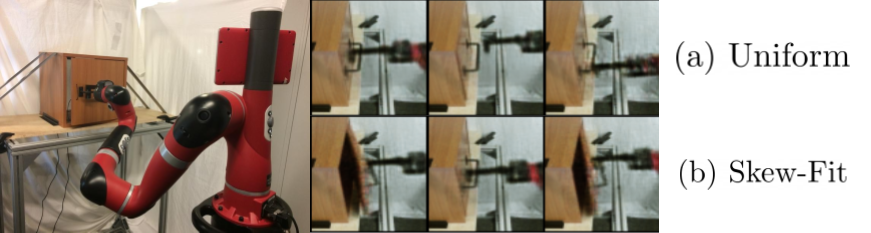
\includegraphics[width=\linewidth]{skewfit/figures/realworldwithsamples.png}
  \caption{
  Left: Robot learning to open a door with \METHOD, without any task reward.
  Right: Samples from a goal distribution when using (a) uniform and (b) \METHOD sampling.
  When used as goals, the diverse samples from \METHOD encourage the robot to practice opening the door more frequently.
  }
  \label{fig:offline-sk-real}
\end{figure}
While reinforcement learning (RL) provides an appealing formalism for automated learning of behavioral skills, separately learning every potentially useful skill becomes prohibitively time consuming, both in terms of the experience required for the agent and the effort required for the user to design reward functions for each behavior.
In the previous chapter, we covered self-supervised goal-conditioned reinforcement learning with a generative model as an approach to scalable multi-task learning with little human supervision.
This approach however, crucially relies on the distribution of data that the generative model is trained on.
What if we could instead design an unsupervised RL algorithm that automatically explores the environment and iteratively distills this experience into general-purpose policies that can accomplish new user-specified tasks at test time?

In the absence of any prior knowledge, an effective exploration scheme is one that visits as many states as possible, allowing a policy to autonomously prepare for user-specified tasks that it might see at test time.
We can formalize the problem of visiting as many states as possible as one of maximizing the \emph{state entropy} $\gH(\SF)$ under the current policy.\stepcounter{footnote}\footnote{We consider the distribution over terminal states in a finite horizon task  and believe this work can be extended to infinite horizon stationary distributions.}
Unfortunately, optimizing this objective alone does not result in a policy that can solve new tasks: it only knows how to maximize state entropy.
In other words, to develop principled unsupervised RL algorithms that result in useful policies, maximizing $\gH(\SF)$ is not enough.
We need a mechanism that allows us to reuse the resulting policy to achieve new tasks at test-time.

We argue that this can be accomplished by performing \textit{goal-directed exploration}:
a policy should autonomously visit as many states as possible, but after autonomous exploration, a user should be able to reuse this policy by giving it a goal $\G$ that corresponds to a state that it must reach.
While not all test-time tasks can be expressed as reaching a goal state, a wide range of tasks can be represented in this way.
Mathematically, the goal-conditioned policy should minimize the conditional entropy over the states given a goal, $\gH(\SF \mid \G)$, so that there is little uncertainty over its state given a commanded goal.
This objective provides us with a principled way to train a policy to explore all states (maximize $\gH(\SF)$) such that the state that is reached can be determined by commanding goals (minimize $\gH(\SF \mid \G)$).

Directly optimizing this objective is in general intractable, since it requires optimizing the entropy of the marginal state distribution, $\gH(\SF)$.
However, we can sidestep this issue by noting that the objective is the mutual information between the state and the goal, $I(\SF; \G)$, which can be written as:
{
  \setlength{\abovedisplayskip}{18pt}%
  \setlength{\belowdisplayskip}{0pt}%
  \setlength{\abovedisplayshortskip}{18pt}%
  \setlength{\belowdisplayshortskip}{0pt}
\begin{align}
    \label{eq:hg-hgs}
    \gH(\SF) - \gH(\SF|\G)
    =
    I(\SF; \G)
    =
    \gH(\G) - \gH(\G|\SF).
\end{align}
}

\Eqref{eq:hg-hgs} thus gives an equivalent objective for an unsupervised RL algorithm:
the agent should set diverse goals, maximizing $\gH(\G)$, and learn how to reach them, minimizing $\gH(\G \mid \SF)$.

While learning to reach goals is the typical objective studied in goal-conditioned RL~\citep{kaelbling1993goals,andrychowicz2017her}, setting goals that have maximum diversity is crucial for effectively learning to reach all possible states.
Acquiring such a maximum-entropy goal distribution is challenging in environments with complex, high-dimensional state spaces, where even knowing which states are valid presents a major challenge.
For example, in image-based domains, a uniform goal distribution requires sampling uniformly from the set of realistic images, which in general is unknown a priori.

In this chapter, we present the following contributions.
First, we propose a principled objective for unsupervised RL, based on \autoref{eq:hg-hgs}.
While a number of prior works ignore the $\gH(\G)$ term, we argue that jointly optimizing the entire quantity is needed to develop effective exploration.
Second, we present a general algorithm called \METHOD and prove that under regularity conditions \METHOD learns a sequence of generative models that converges to a uniform distribution over the goal space, even when the set of valid states is unknown (e.g., as in the case of images).
Third, we describe a concrete implementation of \METHOD and empirically demonstrate that this method achieves state of the art results compared to a large number of prior methods for goal reaching with visually indicated goals, including a real-world manipulation task, which requires a robot to learn to open a door from scratch in about five hours, directly from images, and without any manually-designed reward function.

\setlength{\textfloatsep}{0.5\baselineskip plus 0.2\baselineskip minus 0.2\baselineskip}
\setlength{\dbltextfloatsep}{0.5\baselineskip plus 0.2\baselineskip minus 0.2\baselineskip}

\section{Problem Formulation}\label{sec:background}
To ensure that an unsupervised reinforcement learning agent learns to reach all possible states in a controllable way, we maximize the mutual information between the state $\SF$ and the goal $\G$, $I(\SF; \G)$, as stated in \Eqref{eq:hg-hgs}. This section discusses how to optimize \Eqref{eq:hg-hgs} by splitting the optimization into two parts: minimizing $\gH(\G \mid \SF)$ and maximizing $\gH(\G)$.

\subsection{Minimizing $\gH(\G \mid \SF)$: Goal-Conditioned Reinforcement Learning}
Standard RL considers a Markov decision process (MDP), which has a state space $\Ss$, action space $\As$, and unknown dynamics $\dyn: \Ss \times \Ss \times \As \mapsto [0, +\infty)$.
Goal-conditioned RL also includes a goal space $\Gs$. For simplicity, we will assume in our derivation that the goal space matches the state space, such that $\Gs = \Ss$, though the approach extends trivially to the case where $\Gs$ is a hand-specified subset of $\Ss$, such as the global XY position of a robot.
A goal-conditioned policy $\pi(\at \mid \st, \g)$ maps a state $\st \in \Ss$ and goal $\g \in \Ss$ to a distribution over actions $\at \in \As$, and its objective is to reach the goal, i.e., to make the current state equal to the goal.

Goal-reaching can be formulated as minimizing $\gH(\G \mid \SF)$, and many practical goal-reaching algorithms~\citep{kaelbling1993goals,lillicrap2015continuous, schaul2015uva, andrychowicz2017her, nair2018rig, pong2018tdm,florensa2018selfsupervised} can be viewed as approximations to this objective by observing that the optimal goal-conditioned policy will deterministically reach the goal, resulting in a conditional entropy of zero: $\gH(\G \mid \SF) = 0$.
See \autoref{sec:analysis-appendix} for more details.
Our method may thus be used in conjunction with any of these prior goal-conditioned RL methods in order to jointly minimize $\gH(\G \mid \SF)$ and maximize $\gH(\G)$.

\subsection{Maximizing $\gH(\G)$: Setting Diverse Goals}\label{sec:prelim-max-ent}
We now turn to the problem of setting diverse goals or, mathematically, maximizing the entropy of the goal distribution $\gH(\G)$.
Let $\U$ be the uniform distribution over $\Imgs$, where we assume $\Imgs$ has finite volume so that the uniform distribution is well-defined.
Let $\pg$ be the goal distribution from which goals $\G$ are sampled, parameterized by $\pgparam$.
Our goal is to maximize the entropy of $\pg$, which we write as $\gH(\G)$.
Since the maximum entropy distribution over $\Imgs$ is the uniform distribution $\U$, maximizing $\gH(\G)$ may seem as simple as choosing the uniform distribution to be our goal distribution: $\pg = \U$.
However, this requires knowing the uniform distribution over valid states, which may be difficult to obtain when $\Imgs$ is a subset of $\FullSpace$, for some $\FullSpaceDim$.
For example, if the states correspond to images viewed through a robot's camera, $\Imgs$ corresponds to the (unknown) set of valid images of the robot's environment, while $\FullSpace$ corresponds to all possible arrays of pixel values of a particular size.
In such environments, sampling from the uniform distribution $\FullSpace$ is unlikely to correspond to a valid image of the real world.
Sampling uniformly from $\Imgs$ would require knowing the set of all possible valid images, which we assume the agent does not know when starting to explore the environment.

While we cannot sample arbitrary states from $\Imgs$, we can sample states by performing goal-directed exploration.
To derive and analyze our method, we introduce a simple model of this process:
a goal $\G \sim \pg$ is sampled from the goal distribution $\pg$, and
then the goal-conditioned policy $\pi$ attempts to achieve this goal, which results in a distribution of terminal states $\SF \in \Imgs$.
We abstract this entire process by writing the resulting marginal distribution over $\SF$ as \mbox{$\pstate (\SF) \triangleq \int_\mathcal{G} \pg(\G) p(\SF \mid \G) d\G$}, where the subscript $\pgparam$ indicates that the marginal $\pstate$ depends indirectly on $\pg$ via the goal-conditioned policy $\pi$.
We assume that $\pstate$ has full support, which can be accomplished with an epsilon-greedy goal reaching policy in a communicating MDP.
We also assume that the entropy of the resulting state distribution $\gH(\pstate)$ is no less than the entropy of the goal distribution $\gH(\pg)$.
Without this assumption, a policy could ignore the goal and stay in a single state, no matter how diverse and realistic the goals are.
\footnote{
Note that this assumption does \textbf{not} require that the entropy of $\pstate$ is strictly larger than the entropy of the goal distribution, $\pg$.
}
This simplified model allows us to analyze the behavior of our goal-setting scheme separately from any specific goal-reaching algorithm. We will however show in Section~\ref{sec:experiments} that we can instantiate this approach into a practical algorithm that jointly learns the goal-reaching policy. In summary, our goal is to acquire a maximum-entropy goal distribution $\pg$ over valid states $\Imgs$, while only having access to state samples from $\pstate$.


\section{\METHOD: Learning a Maximum Entropy Goal Distribution}
\label{sec:method}
Our method, \METHOD, learns a maximum entropy goal distribution $\pg$ using samples collected from a goal-conditioned policy.
We analyze the algorithm and show that \METHOD maximizes the goal distribution entropy, and present a practical instantiation for unsupervised deep RL.

\subsection{\METHOD Algorithm}\label{sec:method-description}
To learn a uniform distribution over \emph{valid} goal states, we present a method that iteratively increases the entropy of a generative model $\pg$.
In particular, given a generative model $\pgt$ at iteration $t$, we want to train a new generative model, $\pgtt$ that has higher entropy.
While we do not know the set of valid states $\Imgs$, we could sample states \mbox{$\st_n \overset{\text{iid}}{\sim} \pstatet$} using the goal-conditioned policy,
and use the samples to train $\pgtt$.
However, there is no guarantee that this would increase the entropy of $\pgtt$.

\begin{figure}[ht]
    \centering
    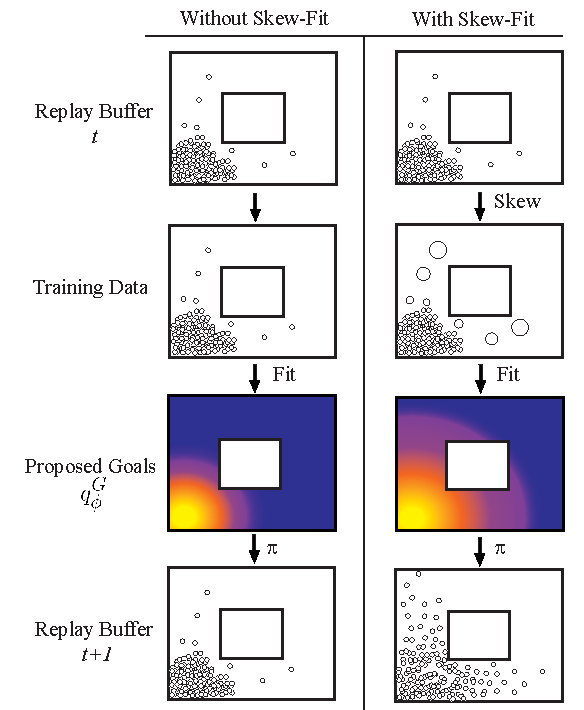
\includegraphics[width=\linewidth]{skewfit/figures/skewfitfigure_vertical_q_phi_g.pdf}
    \fcaption{Our method, \METHOD, samples goals for goal-conditioned RL.
    We sample states from our replay buffer, and give more weight to rare states.
    We then train a generative model $\pg_{t+1}$ with the weighted samples.
    By sampling new states with goals proposed from this new generative model, we obtain a higher entropy state distribution in the next iteration.}
    \label{fig:main-fig}
\end{figure}

The intuition behind our method is simple: rather than fitting a generative model to these samples $\st_n$, we \textit{skew} the samples so that rarely visited states are given more weight.
See \Figref{fig:main-fig} for a visualization of this process.
How should we skew the samples if we want to maximize the entropy of $\pgtt$?
If we had access to the density of each state, $\pet(\St)$, then we could simply weight each state by $1/\pet(\St)$.
We could then perform maximum likelihood estimation (MLE) for the uniform distribution by using the following importance sampling (IS) loss to train $\pgparamtt$:
\begin{align}
\Loss(\pgparam)\nonumber
    &= \E_{\St \sim \U} \left[ \log \pg(\St)\right]
\\\nonumber
    &= \E_{\St \sim \pet}\left[ \frac{\U(\St)}{\pet(\St)} \log \pg(\St)\right]
\\\nonumber
    &\propto \E_{\St \sim \pet}\left[ \frac{1}{\pet(\St)}\log \pg(\St)\right]
\nonumber
\end{align}
where we use the fact that the uniform distribution $\U(\St)$ has constant density for all states in $\Imgs$.
However, computing this density $\pet(\St)$ requires marginalizing out the MDP dynamics, which requires an accurate model of both the dynamics and the goal-conditioned policy.

We avoid needing to model the entire MDP process by approximating $\pet(\St)$ with our previous learned generative model: \mbox{$\pstatet(\St) \approx \pgt(\St)$}.
We therefore weight each state by the following weight function
\begin{align}\label{eq:weight-defn}
    \wt(\SF) \triangleq \pgt(\SF)^\alpha, \quad \alpha < 0.
\end{align}
where $\alpha$ is a hyperparameter that controls how heavily we weight each state.
If our approximation $\pgt$ is exact, we can choose $\alpha = -1$ and recover the exact IS procedure described above.
If $\alpha = 0$, then this skew step has no effect.
By choosing intermediate values of $\alpha$, we trade off the reliability of our estimate $\pgt(\St)$ with the speed at which we want to increase the goal distribution entropy.

\paragraph{Variance Reduction}
As described, this procedure relies on IS, which can have high variance, particularly if $\pgt(\St) \approx 0$.
We therefore choose a class of generative models where the probabilities are prevented from collapsing to zero, as we will describe in \autoref{sec:train-policy} where we provide generative model details.
To further reduce the variance, we train $\pgtt$ with sampling importance resampling (SIR)~\citep{rubin1988using} rather than IS.
Rather than sampling from $\pet$ and weighting the update from each sample by $\wt$, SIR explicitly defines a skewed empirical distribution as
\begin{align}\label{eq:pskew-defn}
    \pskewedt(\st) \triangleq \frac{1}{Z_\alpha} \wt(\st) \delta(\st \in \{\st_n\}_{n=1}^{N})
    \\\nonumber
    Z_\alpha = \sum_{n=1}^N \wt(\st_n),\ \st_n \overset{\text{iid}}{\sim} \pstatet,
\end{align}
where $\delta$ is the indicator function and $Z_\alpha$ is the normalizing coefficient.
We note that computing $Z_\alpha$ adds little computational overhead, since all of the weights already need to be computed.
We then fit the generative model at the next iteration $\pgtt$ to $\pskewedt$ using standard MLE.
We found that using SIR resulted in significantly lower variance than IS.
See \autoref{sec:analysis-variance} for this comparision.

\paragraph{Goal Sampling Alternative}
Because $\pgtt \approx \pskewedt$, at iteration $t+1$, one can sample goals from either $\pgtt$ or $\pskewedt$.
Sampling goals from $\pskewedt$ may be preferred if sampling from the learned generative model $\pgtt$ is computationally or otherwise challenging.
In either case, one still needs to train the generative model $\pgt$ to create $\pskewedt$.
In our experiments, we found that both methods perform well.

\paragraph{Summary}
Overall, \METHOD collects states from the environment and resamples each state in proportion to \autoref{eq:weight-defn} so that low-density states are resampled more often.
\METHOD is shown in \Figref{fig:main-fig} and summarized in Algorithm \ref{alg:method}.
We now discuss conditions under which \METHOD converges to the uniform distribution.

\vspace{0.1in}
\begin{algorithm}
   	\fcaption{\METHOD}
   	\label{alg:method}
   	\begin{algorithmic}[1]
   	\FOR{Iteration $t=1, 2, ...$}
        \STATE Collect $N$ states $\{\st_n\}_{n=1}^N$ by sampling goals from $\pgt$ (or $\pskewed_{t-1}$) and running goal-conditioned policy.
        \STATE Construct skewed distribution $\pskewedt$ (\Eqref{eq:weight-defn} and \Eqref{eq:pskew-defn}).
        \STATE Fit $\pgtt$ to skewed distribution $\pskewedt$ using MLE.
   	\ENDFOR
   	\end{algorithmic}
\end{algorithm}

\subsection{\METHOD Analysis}\label{sec:analysis}
This section provides conditions under which $\pgt$ converges in the limit to the uniform distribution over the state space $\Imgs$.
We consider the case where $N \rightarrow \infty$, which allows us to study the limit behavior of the goal distribution $\pskewedt$.
Our most general result is stated as follows:
\begin{lemma}\label{lemma:general-convergence}
Let $\Imgs$ be a compact set.
Define the set of distributions $\gQ = \{p : \support(p) \subseteq \Imgs\}$.
Let $\gF: \gQ \mapsto \gQ$ be continuous with respect to the pseudometric \mbox{$\dent(p, q) \triangleq |\gH(p) - \gH(q)|$} and $\gH(\gF(p)) \geq \gH(p)$ with equality if and only if $p$ is the uniform probability distribution on $\Imgs$, denoted as $\U$.
Define the sequence of distributions $P = (p_1, p_2, \dots)$ by starting with any $p_1 \in \gQ$ and recursively defining $p_{t+1} = \gF(p_t)$.
The sequence $P$ converges to $\U$ with respect to $\dent$. In other words, \mbox{$\lim_{t \rightarrow 0} |\gH(p_t) - \gH(\U)| \rightarrow 0$}.
\end{lemma}
\begin{proof}
See Appendix Section \ref{sec:general-proof}.
\end{proof}

We will apply Lemma \ref{lemma:general-convergence} to be the map from $\pskewedt$ to $\pskewedtt$ to show that $\pskewedt$ converges to $\U$.
If we assume that the goal-conditioned policy and generative model learning procedure are well behaved
(i.e., the maps from $\pgt$ to $\pet$ and from $\pskewedt$ to $\pgtt$ are continuous),
then to apply Lemma~\ref{lemma:general-convergence}, we only need to show that \mbox{$\gH(\pskewedt) \geq \gH(\pet)$} with equality if and only if \mbox{$\pet = \U$}.
For the simple case when \mbox{$\pgt = \pet$} identically at each iteration, we prove the convergence of \METHOD true for any value of $\alpha \in [-1, 0)$ in \autoref{sec:simple-case-proof}.
However, in practice, $\pgt$ only approximates $\pet$. To address this more realistic situation, we prove the following result:
\begin{lemma}\label{lemma:pos-cov-negative-grad}
Given two distribution $\pet$ and $\pgt$ where $\pet \ll \pgt$
\footnote{
$p \ll q$ means that $p$ is absolutely continuous with respect to $q$, i.e. $p(\st) = 0 \implies q(\st) = 0$.
}
and
\begin{align}\label{eq:pos-cov}
  \Cov_{\St \sim \pet}\left[\log \pet(\St), \log \pgt(\St)\right] > 0,
\end{align}
define the $\pskewedt$ as in \Eqref{eq:pskew-defn} and take $N \rightarrow \infty$.
Let $\gH_\alpha(\alpha)$ be the entropy of $\pskewedt$ for a fixed $\alpha$.
Then there exists a constant $a < 0$ such that for all $\alpha \in [a, 0)$,
\begin{align*}
    \gH(\pskewedt) =  \gH_\alpha(\alpha) > \gH(\pet).
\end{align*}
\end{lemma}
\begin{proof}
See Appendix Section \ref{sec:covariance-proof}.
\end{proof}
This lemma tells us that our generative model $\pgt$ does not need to exactly fit the sampled states.
Rather, we merely need the log densities of $\pgt$ and $\pet$ to be correlated, which we expect to happen frequently with an accurate goal-conditioned policy, since $\pet$ is the set of states seen when trying to reach goals from $\pgt$.
In this case, if we choose negative values of $\alpha$ that are small enough, then the entropy of $\pskewedt$ will be higher than that of $\pet$.
Empirically, we found that $\alpha$ values as low as $\alpha=-1$ performed well.

In summary, $\pskewedt$ converges to $\U$ under certain assumptions.
Since we train each generative model $\pgtt$ by fitting it to $\pskewedt$ with MLE, $\pgt$ will also converge to $\U$.


\section{Training Goal-Conditioned Policies with \METHOD}
\label{sec:train-policy}
Thus far, we have presented \METHOD assuming that we have access to a goal-reaching policy, allowing us to separately analyze how we can maximize $\HG$.
However, in practice we do not have access to such a policy, and this section discusses how we concurrently train a goal-reaching policy.

Maximizing $I(\SF; \G)$ can be done by simultaneously performing \METHOD and training a goal-conditioned policy to minimize $\HGS$, or, equivalently, maximize $-\HGS$.
Maximizing $-\HGS$ requires computing the density $\log p(\G \mid \SF)$, which may be difficult to compute without strong modeling assumptions.
However, for any distribution $q$, the following lower bound on $-\HGS$:
\begin{align}\nonumber
-\HGS
    &= \E_{(\G, \SF) \sim q}\left[
        \log q(\G \mid \SF)
    \right]
+ \kld{p}{q}
\\\nonumber
&
    \geq \E_{(\G, \SF) \sim q}\left[
        \log q(\G \mid \SF)
    \right],
\end{align}
where $\KL$ denotes Kullback–Leibler divergence as discussed by \citet{barber2004information}.
Thus, to minimize $\HGS$, we train a policy to maximize the reward
\begin{align}\nonumber
    r(\SF, \G) = \log q(\G \mid \SF).
\end{align}

The RL algorithm we use is reinforcement learning with imagined goals (RIG)~\citep{nair2018rig}, though in principle any goal-conditioned method could be used.
RIG is an efficient off-policy goal-conditioned method that solves vision-based RL problems in a learned latent space.
In particular, RIG fits a $\beta$-VAE~\citep{higgins2016beta} and uses it to encode observations and goals into a latent space, which it uses as the state representation.
RIG also uses the $\beta$-VAE to compute rewards, $\log q(\G \mid \SF)$.
Unlike RIG, we use the goal distribution from \METHOD to sample goals for exploration and for relabeling goals during training~\citep{andrychowicz2017her}.
Since RIG already trains a generative model over states, we reuse this $\beta$-VAE for the generative model $\pg$ of \METHOD.
To make the most use of the data, we train $\pg$ on all visited state rather than only the terminal states, which we found to work well in practice.
To prevent the estimated state likelihoods from collapsing to zero, we model the posterior of the $\beta$-VAE as a multivariate Gaussian distribution with a fixed variance and only learn the mean.
We summarize RIG and provide details for how we combine \METHOD and RIG in \autoref{sec:rig-and-full-method} and describe how we estimate the likelihoods given the $\beta$-VAE in \autoref{sec:likelihood-estimation-vae}.


\section{Related Work}\label{sec:related_work}
Many prior methods in the goal-conditioned reinforcement learning literature focus on training goal-conditioned policies and assume that a goal distribution is available to sample from during exploration~\citep{kaelbling1993goals,schaul2015uva,andrychowicz2017her,pong2018tdm}, or use a heuristic to design a non-parametric~\citep{colas2018gep,wardefarley2018discern,florensa2018selfsupervised} or parametric~\citep{pere2018unsupervised,nair2018rig} goal distribution based on previously visited states.
These methods are largely complementary to our work:
rather than proposing a better method for training goal-reaching policies, we propose a principled method for maximizing the entropy of a goal sampling distribution, $\gH(\G)$, such that these policies cover a wide range of states.

Our method learns without any task rewards, directly acquiring a policy that can be reused to reach user-specified goals.
This stands in contrast to exploration methods that modify the reward based on state visitation frequency~\citep{bellemare2016unifying,ostrovski2017count,tang2017hashtag,chentanez2005intrinsically,lopes2012exploration,stadie2016exploration,pathak2017curiosity,burda2018exploration,burda2018large,mohamed2015variational,tang2017hashtag,fu2017ex2}.
While these methods can also be used without a task reward, they provide no mechanism for distilling the knowledge gained from visiting diverse states into flexible policies that can be applied to accomplish new goals at test-time: their policies visit novel states, and they quickly forget about them as other states become more novel.
Similarly, methods that provably maximize state entropy without using goal-directed exploration~\citep{hazan2019provably} or methods that define new rewards to capture measures of intrinsic motivation~\citep{mohamed2015variational} and reachability~\citep{savinov2018episodic} do not produce reusable policies.

Other prior methods extract reusable skills in the form of latent-variable-conditioned policies, where
latent variables are interpreted as options~\citep{sutton1999between} or abstract skills~\citep{hausman2018skillembedding,gupta2018structuredexploration,eysenbach2018diayn,gupta2018unsupervised,florensa2017stochastic}.
The resulting skills are diverse, but have no grounded interpretation, while \METHOD policies can be used immediately after unsupervised training to reach diverse user-specified goals.

Some prior methods propose to choose goals based on heuristics such as learning progress~\citep{baranes2012, veeriah2018many, colas2018curious}, how off-policy the goal is~\citep{nachum2018hiro}, level of difficulty~\citep{held2018goalgan}, or likelihood ranking~\citep{zhao2019rankweight}.
In contrast, our approach provides a principled framework for optimizing a concrete and well-motivated exploration objective, can provably maximize this objective under regularity assumptions, and empirically outperforms many of these prior work (see \autoref{sec:experiments}).

\section{Experiments}\label{sec:experiments}
Our experiments study the following questions:
\textbf{(1)} Does \METHOD empirically result in a goal distribution with increasing entropy?
\textbf{(2)} Does \METHOD improve exploration for goal-conditioned RL?
\textbf{(3)} How does \METHOD compare to prior work on choosing goals for vision-based, goal-conditioned RL?
\textbf{(4)} Can \METHOD be applied to a real-world, vision-based robot task?

\begin{figure}[t]
    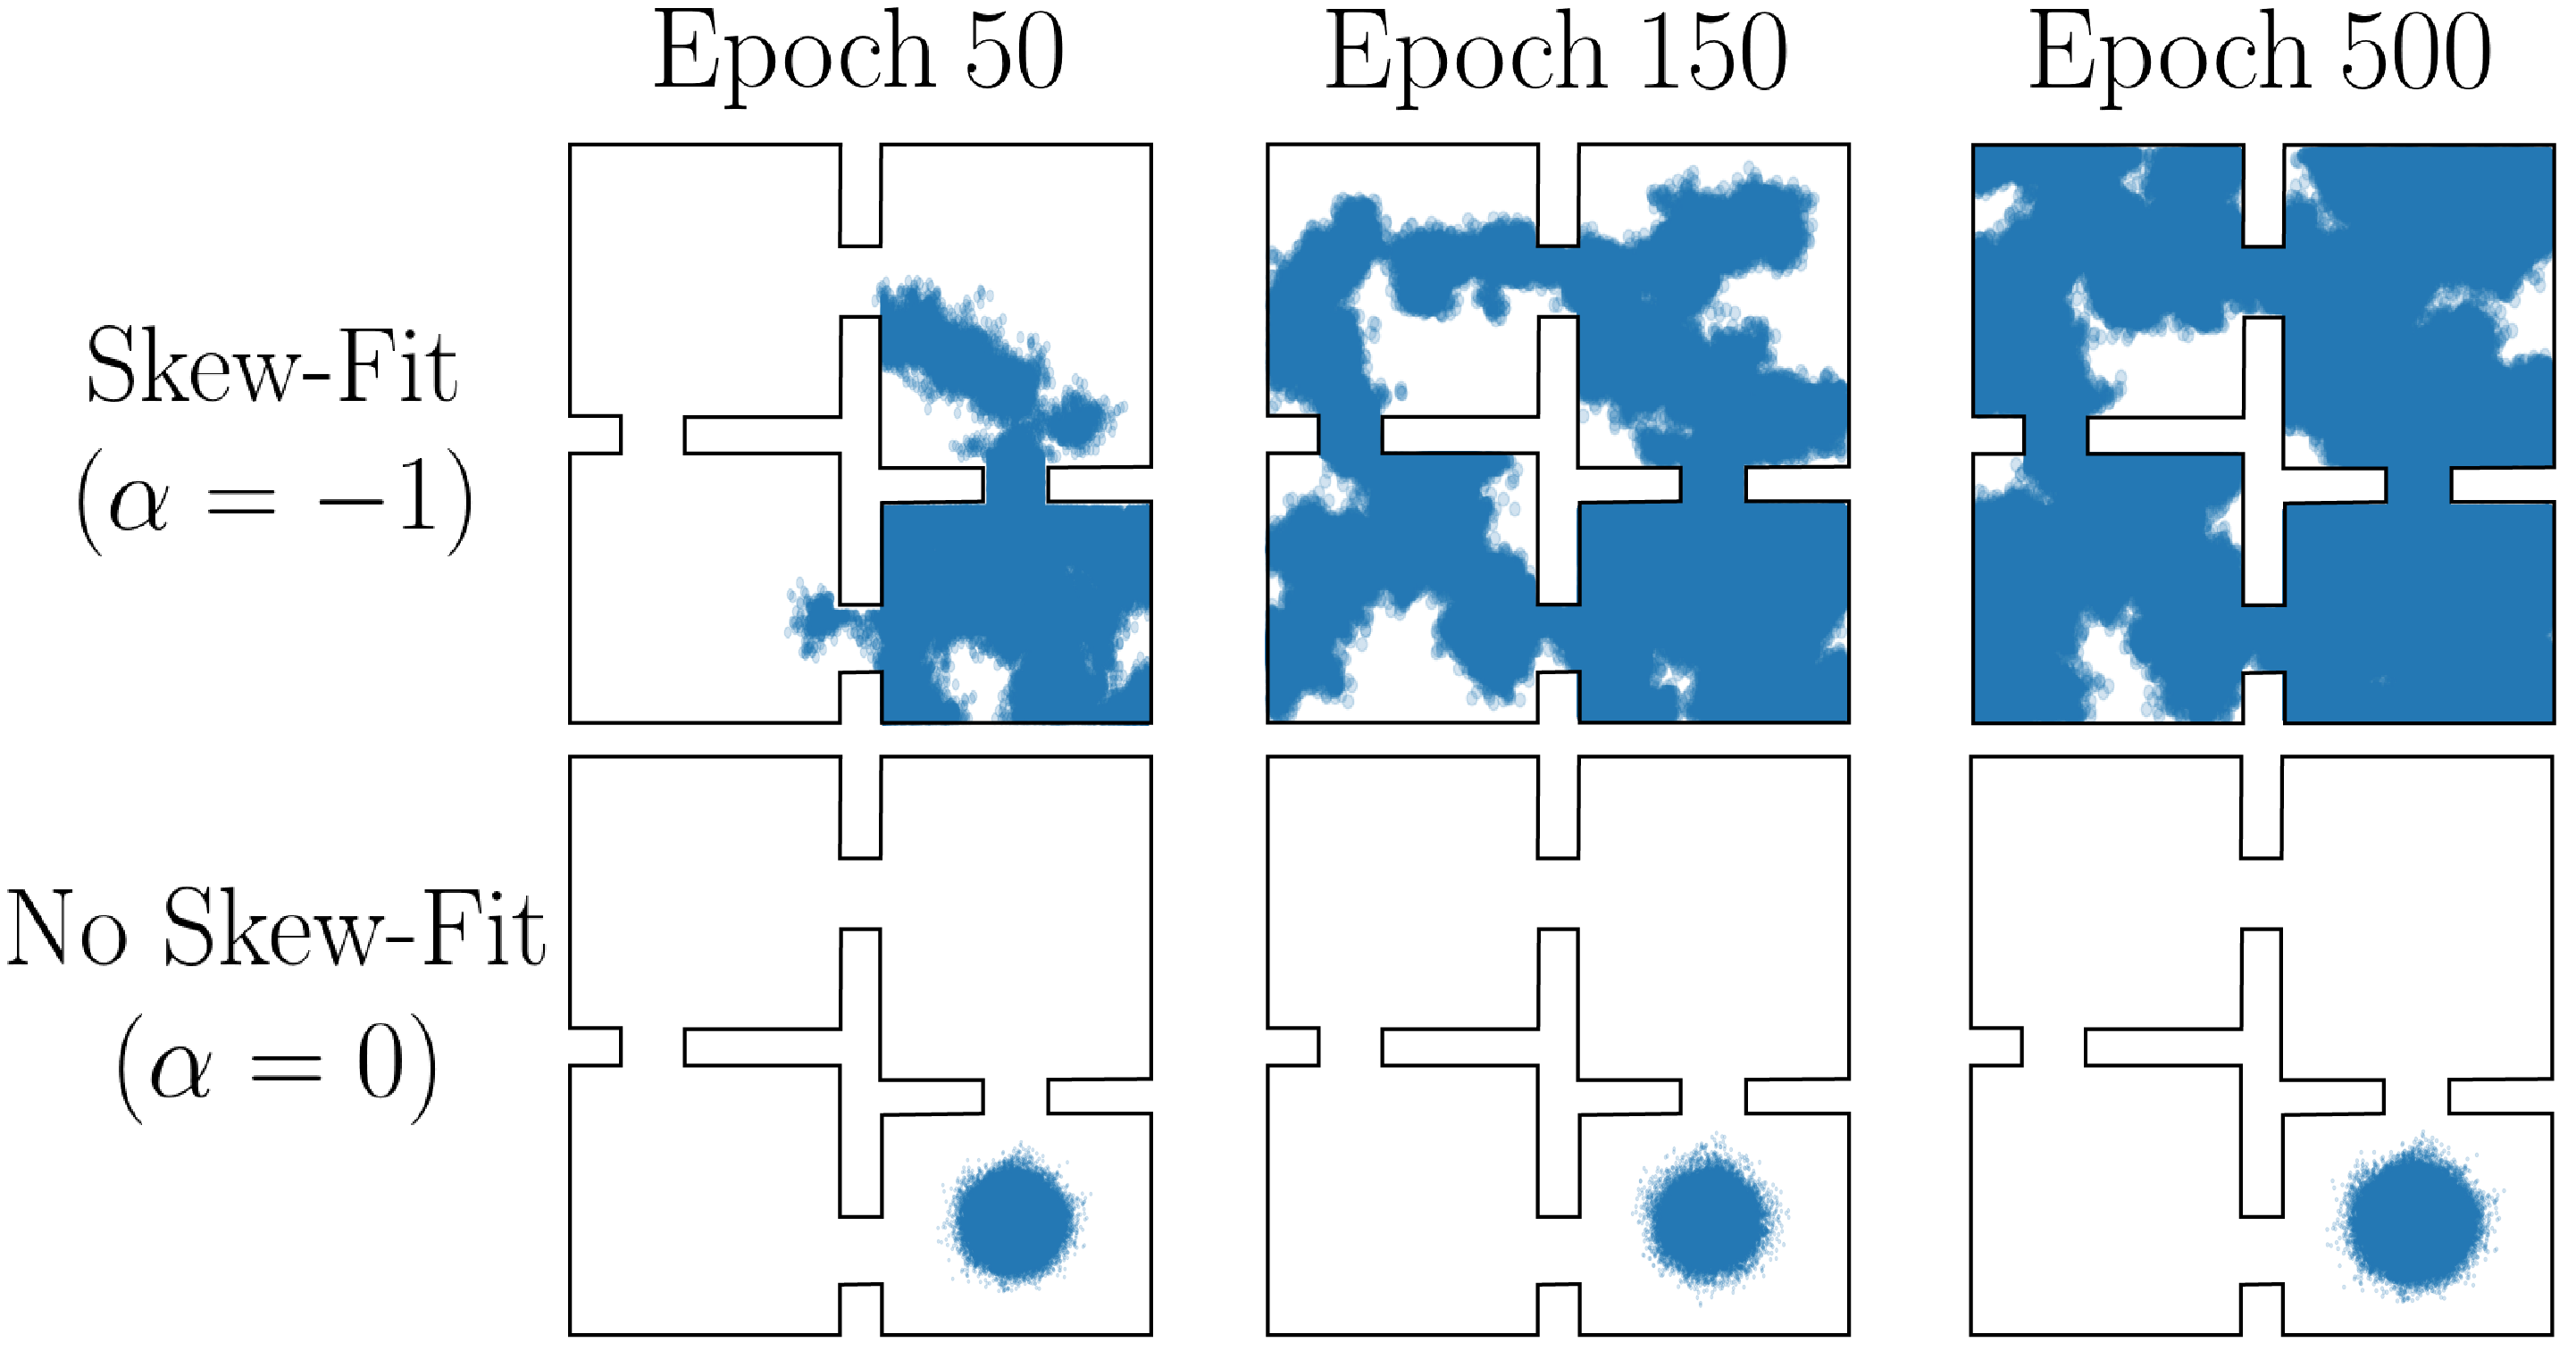
\includegraphics[width=.49\linewidth ]{skewfit/figures/entropy_figure-01.png}
    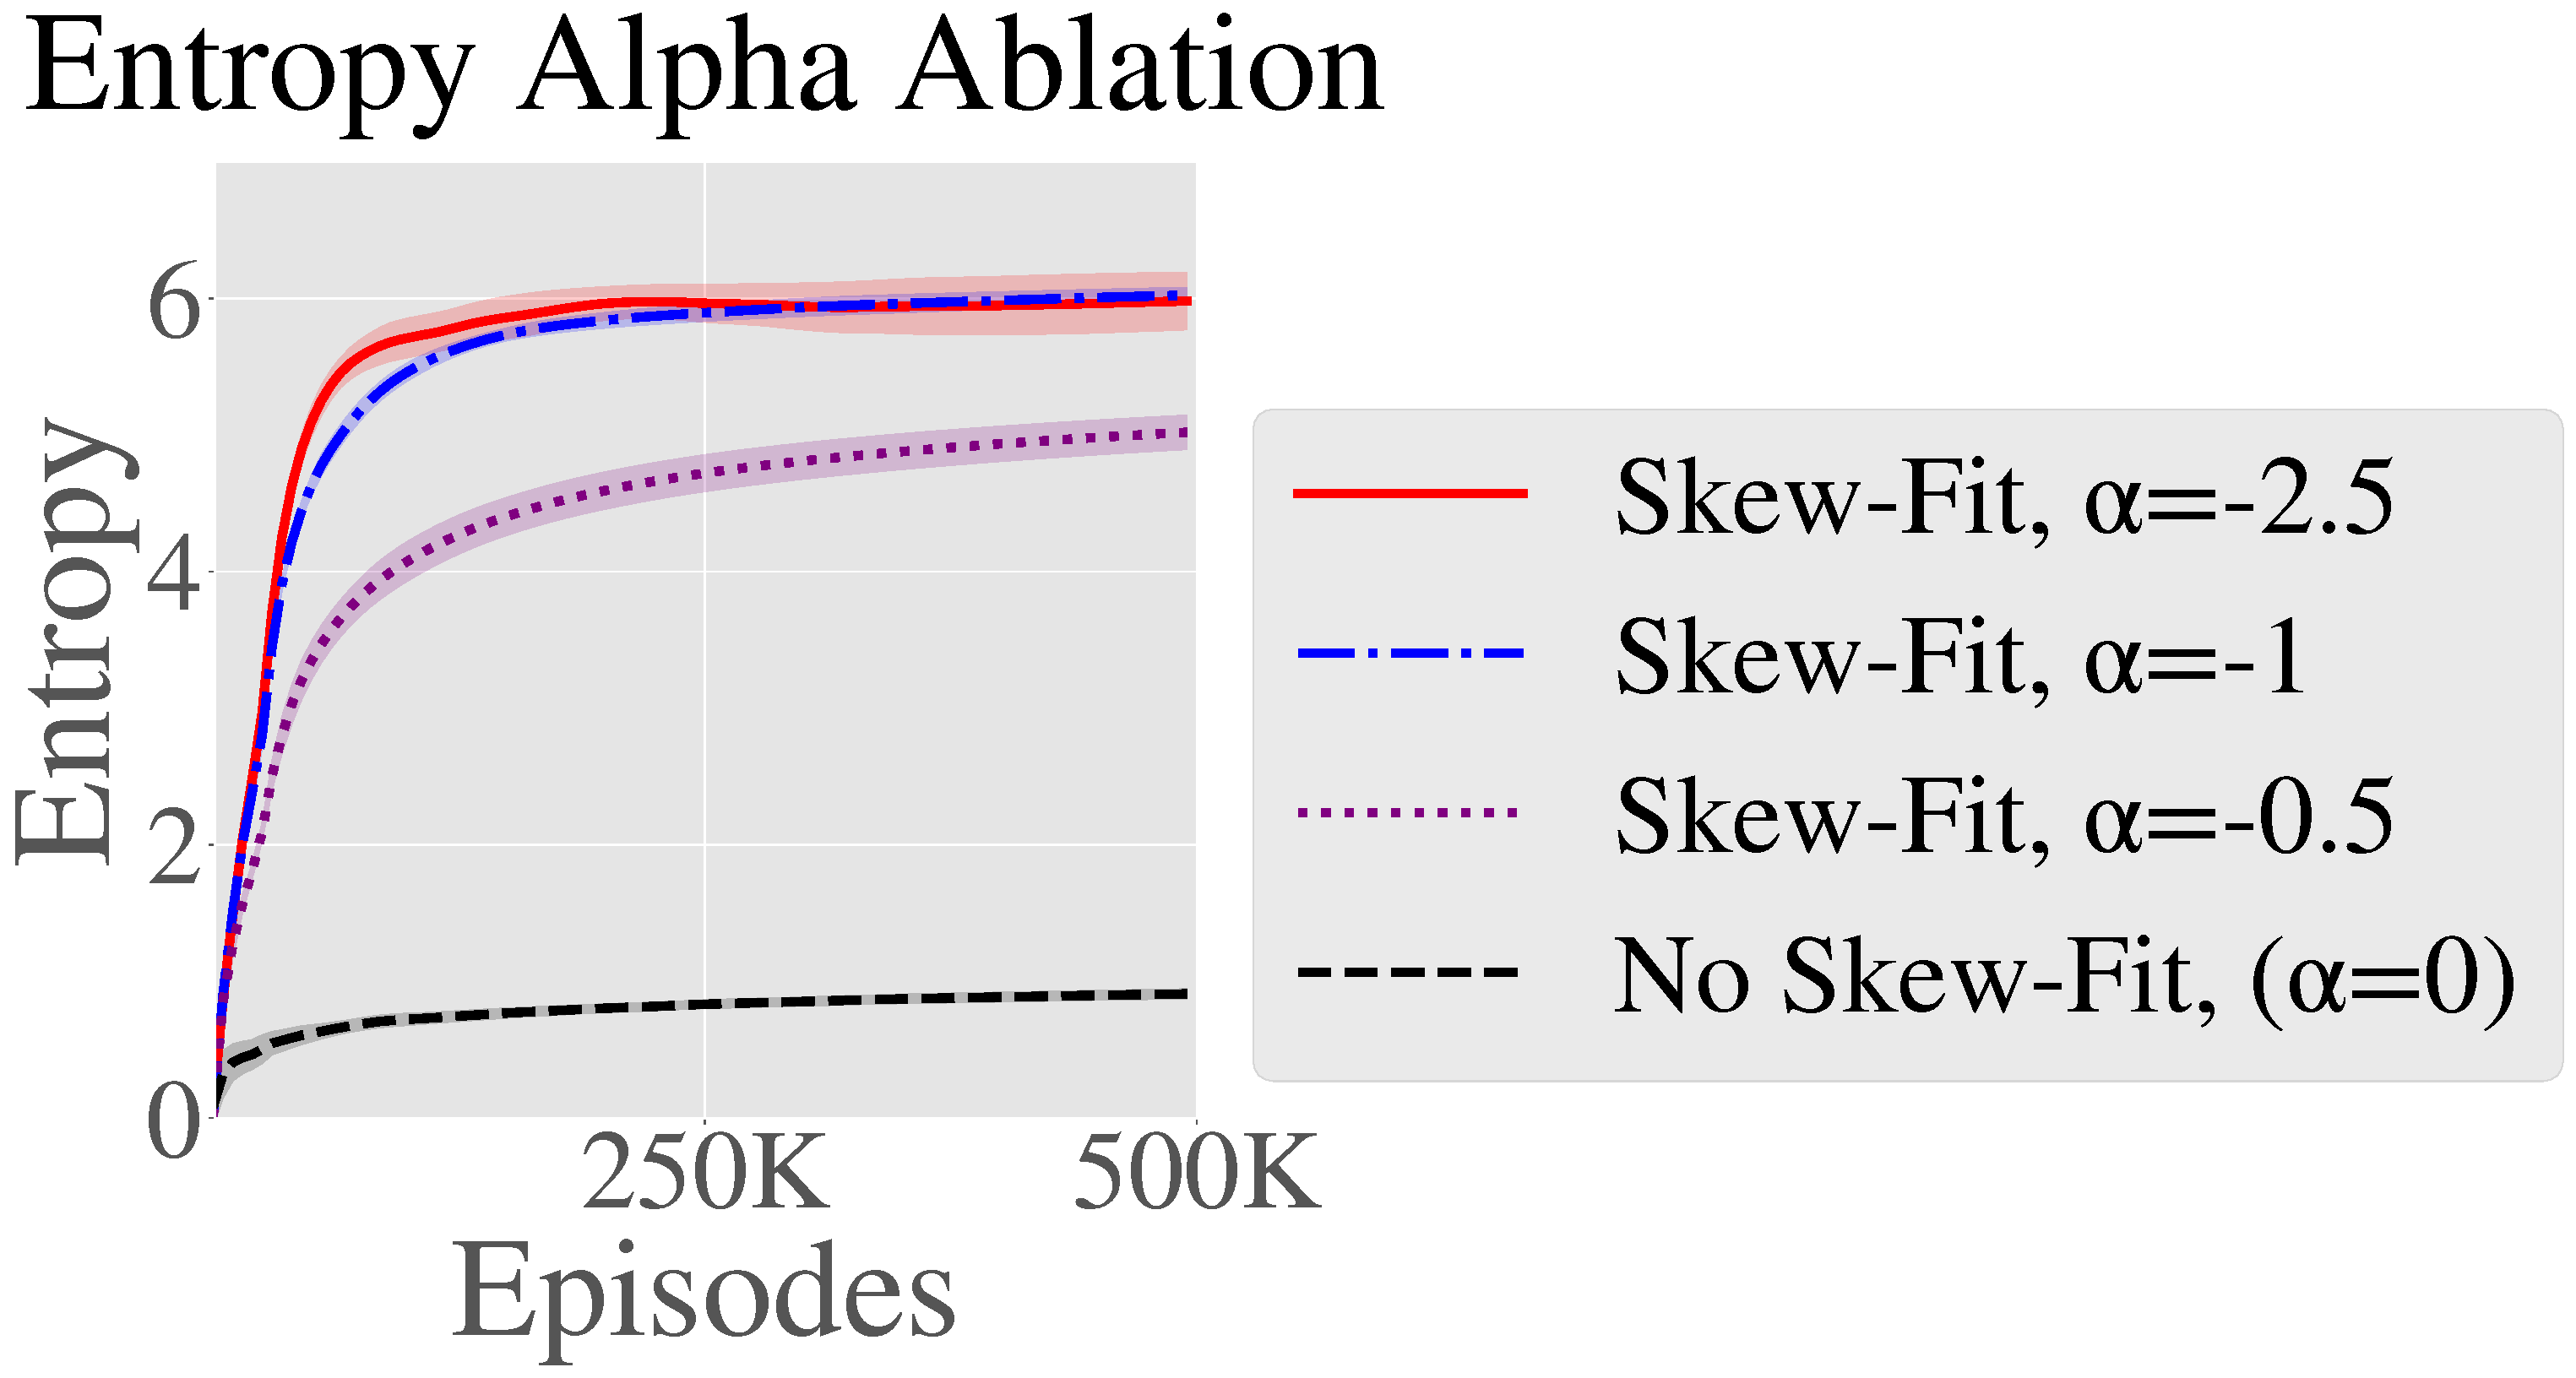
\includegraphics[width=.49\linewidth ]{skewfit/figures/plots/four_rooms_entropy}
    \fcaption{
    Illustrative example of \METHOD on a 2D navigation task. (Left) Visited state plot for \METHOD with $\alpha = -1$ and uniform sampling, which corresponds to $\alpha = 0$. (Right) The entropy of the goal distribution per iteration, mean and standard deviation for 9 seeds. Entropy is calculated via discretization onto an 11x11 grid. \METHOD steadily increases the state entropy, reaching full coverage over the state space.
    }
    \label{fig:2d-sl}
\end{figure}

\paragraph{Does \METHOD Maximize Entropy?}
To see the effects of \METHOD on goal distribution entropy in isolation of learning a goal-reaching policy, we study an idealized example where the policy is a near-perfect goal-reaching policy.
The environment consists of four rooms~\citep{sutton1999between}.
At the beginning of an episode, the agent begins in the bottom-right room and samples a goal from the goal distribution $\pgt$.
To simulate stochasticity of the policy and environment, we add a Gaussian noise with standard deviation of $0.06$ units to this goal, where the entire environment is $11 \times 11$ units.
The policy reaches the state that is closest to this noisy goal and inside the rooms, giving us a state sample $\st_n$ for training $\pgt$.
Due to the relatively small noise, the agent cannot rely on this stochasticity to explore the different rooms and must instead learn to set goals that are progressively farther and farther from the initial state.
We compare multiple values of $\alpha$, where $\alpha=0$ corresponds to not using \METHOD.
The $\beta$-VAE hyperparameters used to train $\pgt$ are given in \autoref{sec:2d-details}.
As seen in \Figref{fig:2d-sl}, sampling uniformly from previous experience ($\alpha = 0$) to set goals results in a policy that primarily sets goal near the initial state distribution.
In contrast, \METHOD results in quickly learning a high entropy, near-uniform distribution over the state space.

\begin{figure}[t]
    \centering
    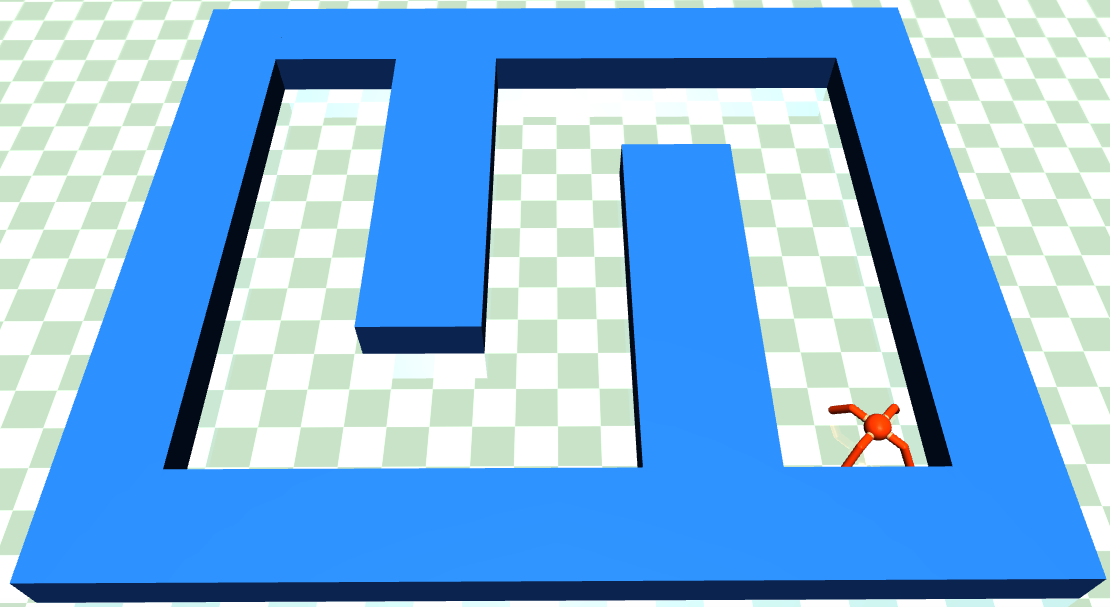
\includegraphics[width=0.32\linewidth]{skewfit/figures/ant_env_updated.png}
    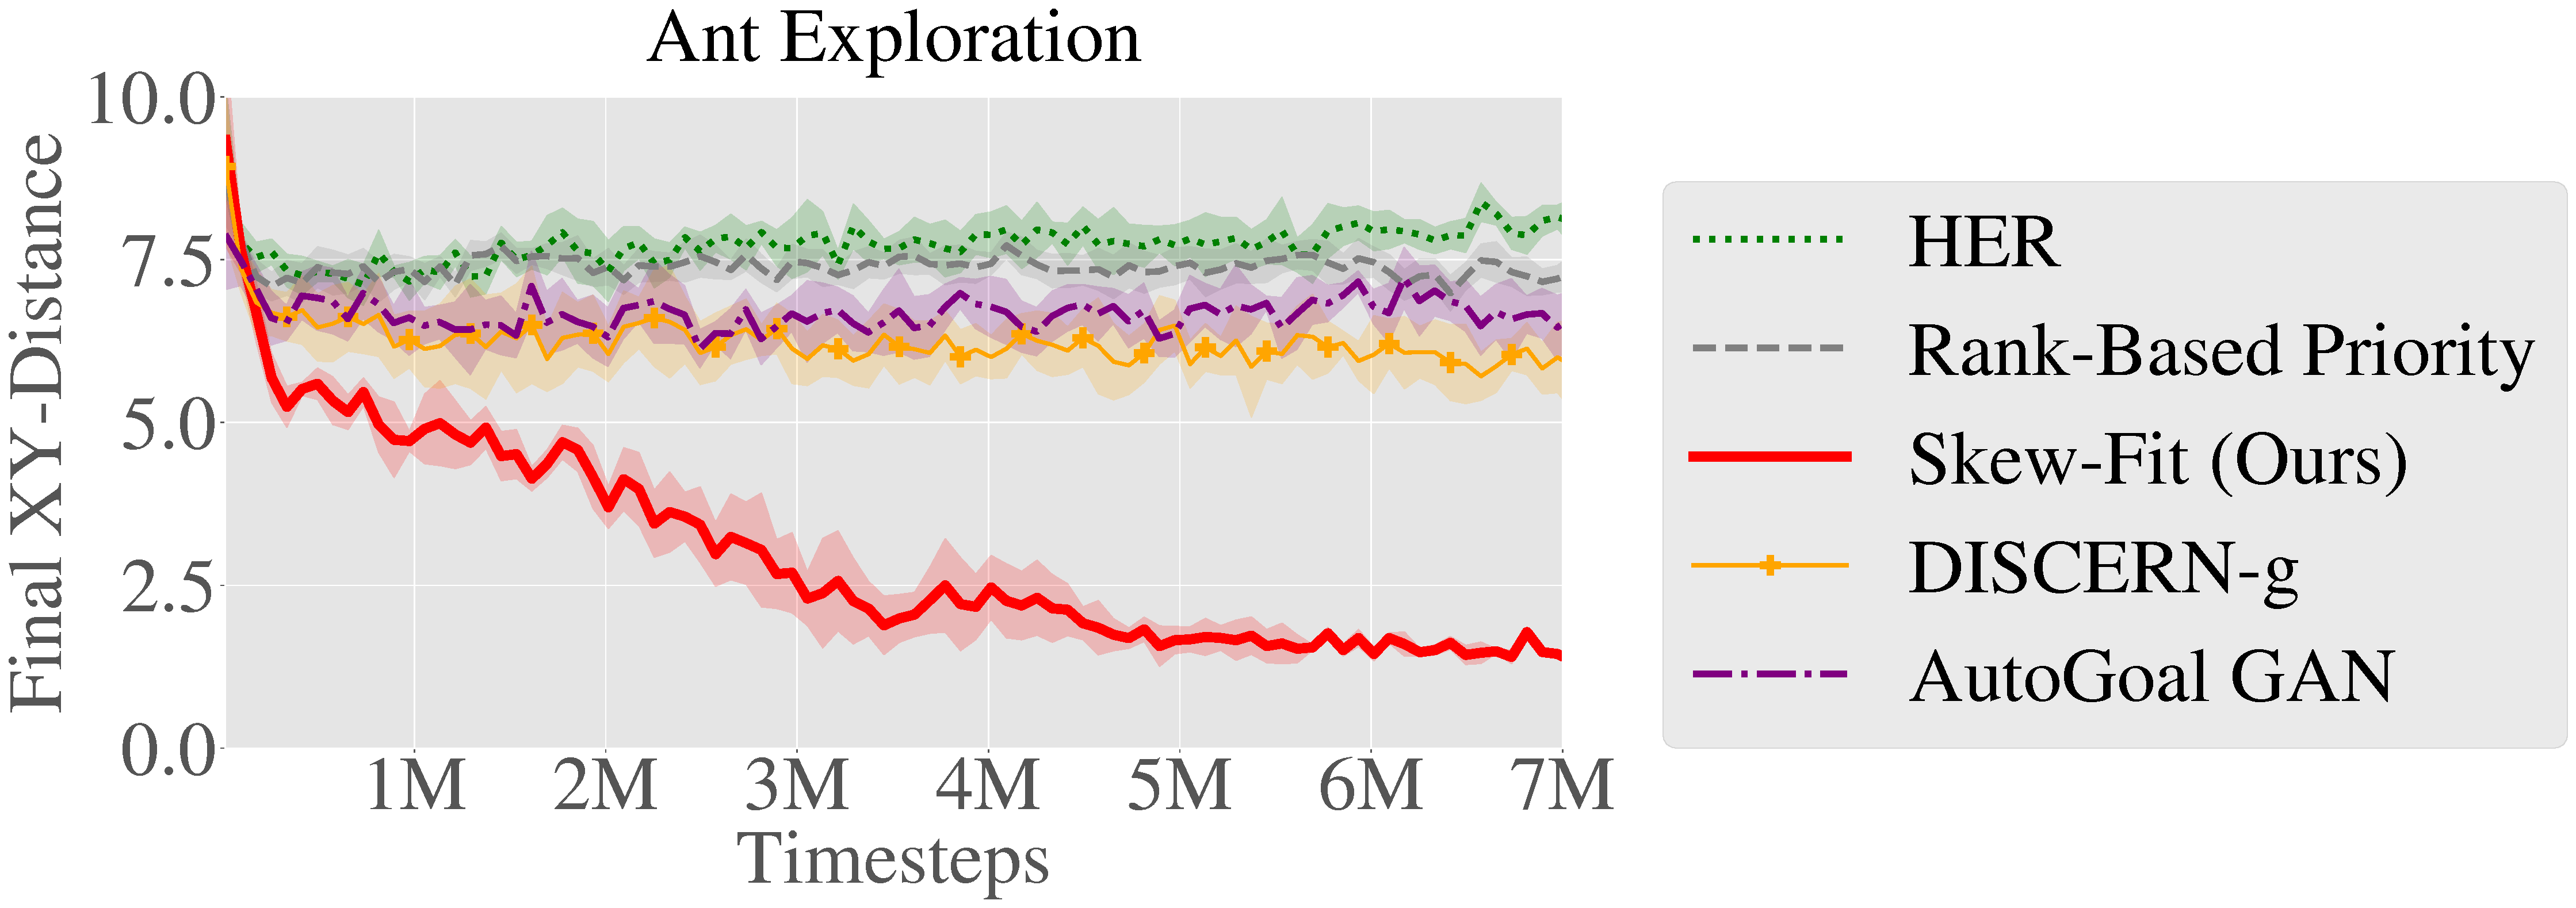
\includegraphics[width=0.65\linewidth]{skewfit/figures/plots/ant.pdf}
    \fcaption{
    (Left) Ant navigation environment.
    (Right) Evaluation on reaching target XY position.
    We show the mean and standard deviation of 6 seeds.
    \METHOD significantly outperforms prior methods on this exploration task.
    }
    \label{fig:antmaze}
\end{figure}

\paragraph{Exploration with \METHOD}
We next evaluate \METHOD while concurrently learning a goal-conditioned policy on a task with state inputs, which enables us study exploration performance independently of the challenges with image observations.
We evaluate on a task that requires training a simulated quadruped ``ant'' robot to navigate to different XY positions in a labyrinth,
as shown in \Figref{fig:antmaze}.
The reward is the negative distance to the goal XY-position, and additional environment details are provided in \autoref{sec:environment-details}.
This task presents a challenge for goal-directed exploration:
the set of valid goals is unknown due to the walls, and
random actions do not result in exploring locations far from the start.
Thus, \METHOD must set goals that meaningfully explore the space while simultaneously learning to reach those goals.

We use this domain to compare \METHOD to a number of existing goal-sampling methods.
We compare to the relabeling scheme described in the hindsight experience replay (labeled \textbf{HER}).
We compare to curiosity-driven prioritization (\textbf{Ranked-Based Priority})~\citep{zhao2019maximum}, a variant of HER that samples goals for relabeling based on their ranked likelihoods.
\citet{held2018goalgan} samples goals from a GAN based on the difficulty of reaching the goal.
We compare against this method by replacing $\pg$ with the GAN and label it \textbf{AutoGoal GAN}.
We also compare to the non-parametric goal proposal mechanism proposed by \cite{wardefarley2018discern}, which we label \textbf{DISCERN-g}.
Lastly, to demonstrate the difficulty of the exploration challenge in these domains, we compare to \textbf{\#-Exploration}~\citep{tang2017hashtag}, an exploration method that assigns bonus rewards based on the novelty of new states.
We train the goal-conditioned policy for each method using soft actor critic (SAC)~\citep{haarnoja2018sacapp}.
Implementation details of SAC and the prior works are given in  \autoref{sec:prior-work-implementation}.

We see in \Figref{fig:antmaze} that \METHOD is the only method that makes significant progress on this challenging labyrinth locomotion task.
The prior methods on goal-sampling primarily set goals close to the start location, while the extrinsic exploration reward in \#-Exploration dominated the goal-reaching reward.
These results demonstrate that \METHOD accelerates exploration by setting diverse goals in tasks with unknown goal spaces.


\paragraph{Vision-Based Continuous Control Tasks}
\begin{figure}[t]
    \centering
    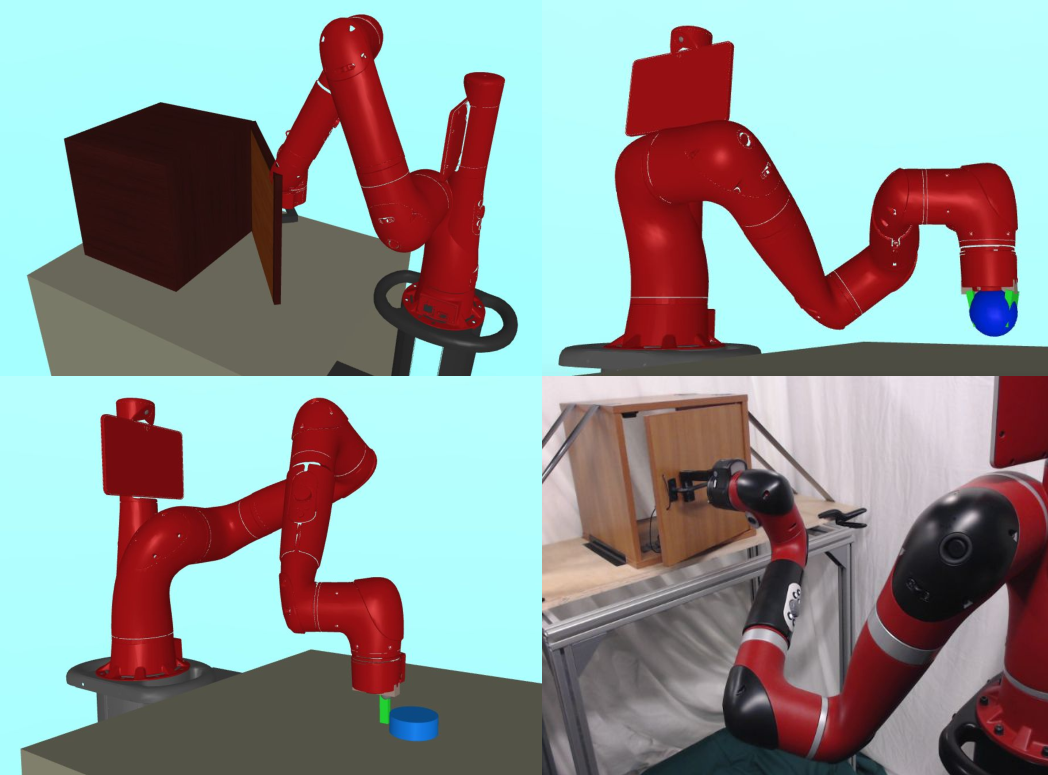
\includegraphics[width=0.8\linewidth]{skewfit/figures/env_display.pdf}
    \fcaption{We evaluate on these continuous control tasks, from left to right:
    \textit{Visual Door}, a door opening task;
    \textit{Visual Pickup}, a picking task;
    \textit{Visual Pusher}, a pushing task;
    and \textit{Real World Visual Door}, a real world door opening task. All tasks are solved from images and without any task-specific reward. See Appendix \ref{sec:environment-details} for details.}
    \label{fig:env-pics}
\end{figure}

We now evaluate \METHOD on a variety of image-based continuous control tasks, where the policy must control a robot arm using only image observations, there is no state-based or task-specific reward, and \METHOD must directly set image goals.
We test our method on three different image-based simulated continuous control tasks released by the authors of RIG~\citep{nair2018rig}: \textit{Visual Door}, \textit{Visual Pusher}, and \textit{Visual Pickup}.
These environments contain a robot that can open a door, push a puck, and lift up a ball to different configurations, respectively.
To our knowledge, these are the only goal-conditioned, vision-based continuous control environments that are publicly available and experimentally evaluated in prior work, making them a good point of comparison.
See \autoref{fig:env-pics} for visuals and \autoref{sec:implementation-details} for environment details.
The policies are trained in a completely unsupervised manner, without access to any prior information about the image-space or any pre-defined goal-sampling distribution.
To evaluate their performance, we sample goal images from a uniform distribution over valid states and report the agent's final distance to the corresponding simulator states (e.g., distance of the object to the target object location), but the agent never has access to this true uniform distribution nor the ground-truth state information during training.
While this evaluation method is only practical in simulation, it provides us with a quantitative measure of a policy's ability to reach a broad coverage of goals in a vision-based setting.

We compare \METHOD to a number of existing methods on this domain.
First, we compare to the methods described in the previous experiment (HER, Rank-Based Priority, \#-Exploration, Autogoal GAN, and \mbox{DISCERN-g}).
These methods that we compare to were developed in non-vision, state-based environments.
To ensure a fair comparison across methods, we combine these prior methods with a policy trained using RIG.
We additionally compare to \citet{hazan2019provably}, an exploration method that assigns bonus rewards based on the likelihood of a state (labeled \textbf{Hazan et al.}).
Next, we compare to \textbf{RIG} without \METHOD.
Lastly, we compare to \textbf{DISCERN}~\citep{wardefarley2018discern}, a vision-based method which uses a non-parametric clustering approach to sample goals and an image discriminator to compute rewards.

\begin{figure}
    \centering
     \begin{subfigure}[t]{.49\linewidth}
    \centering
        % 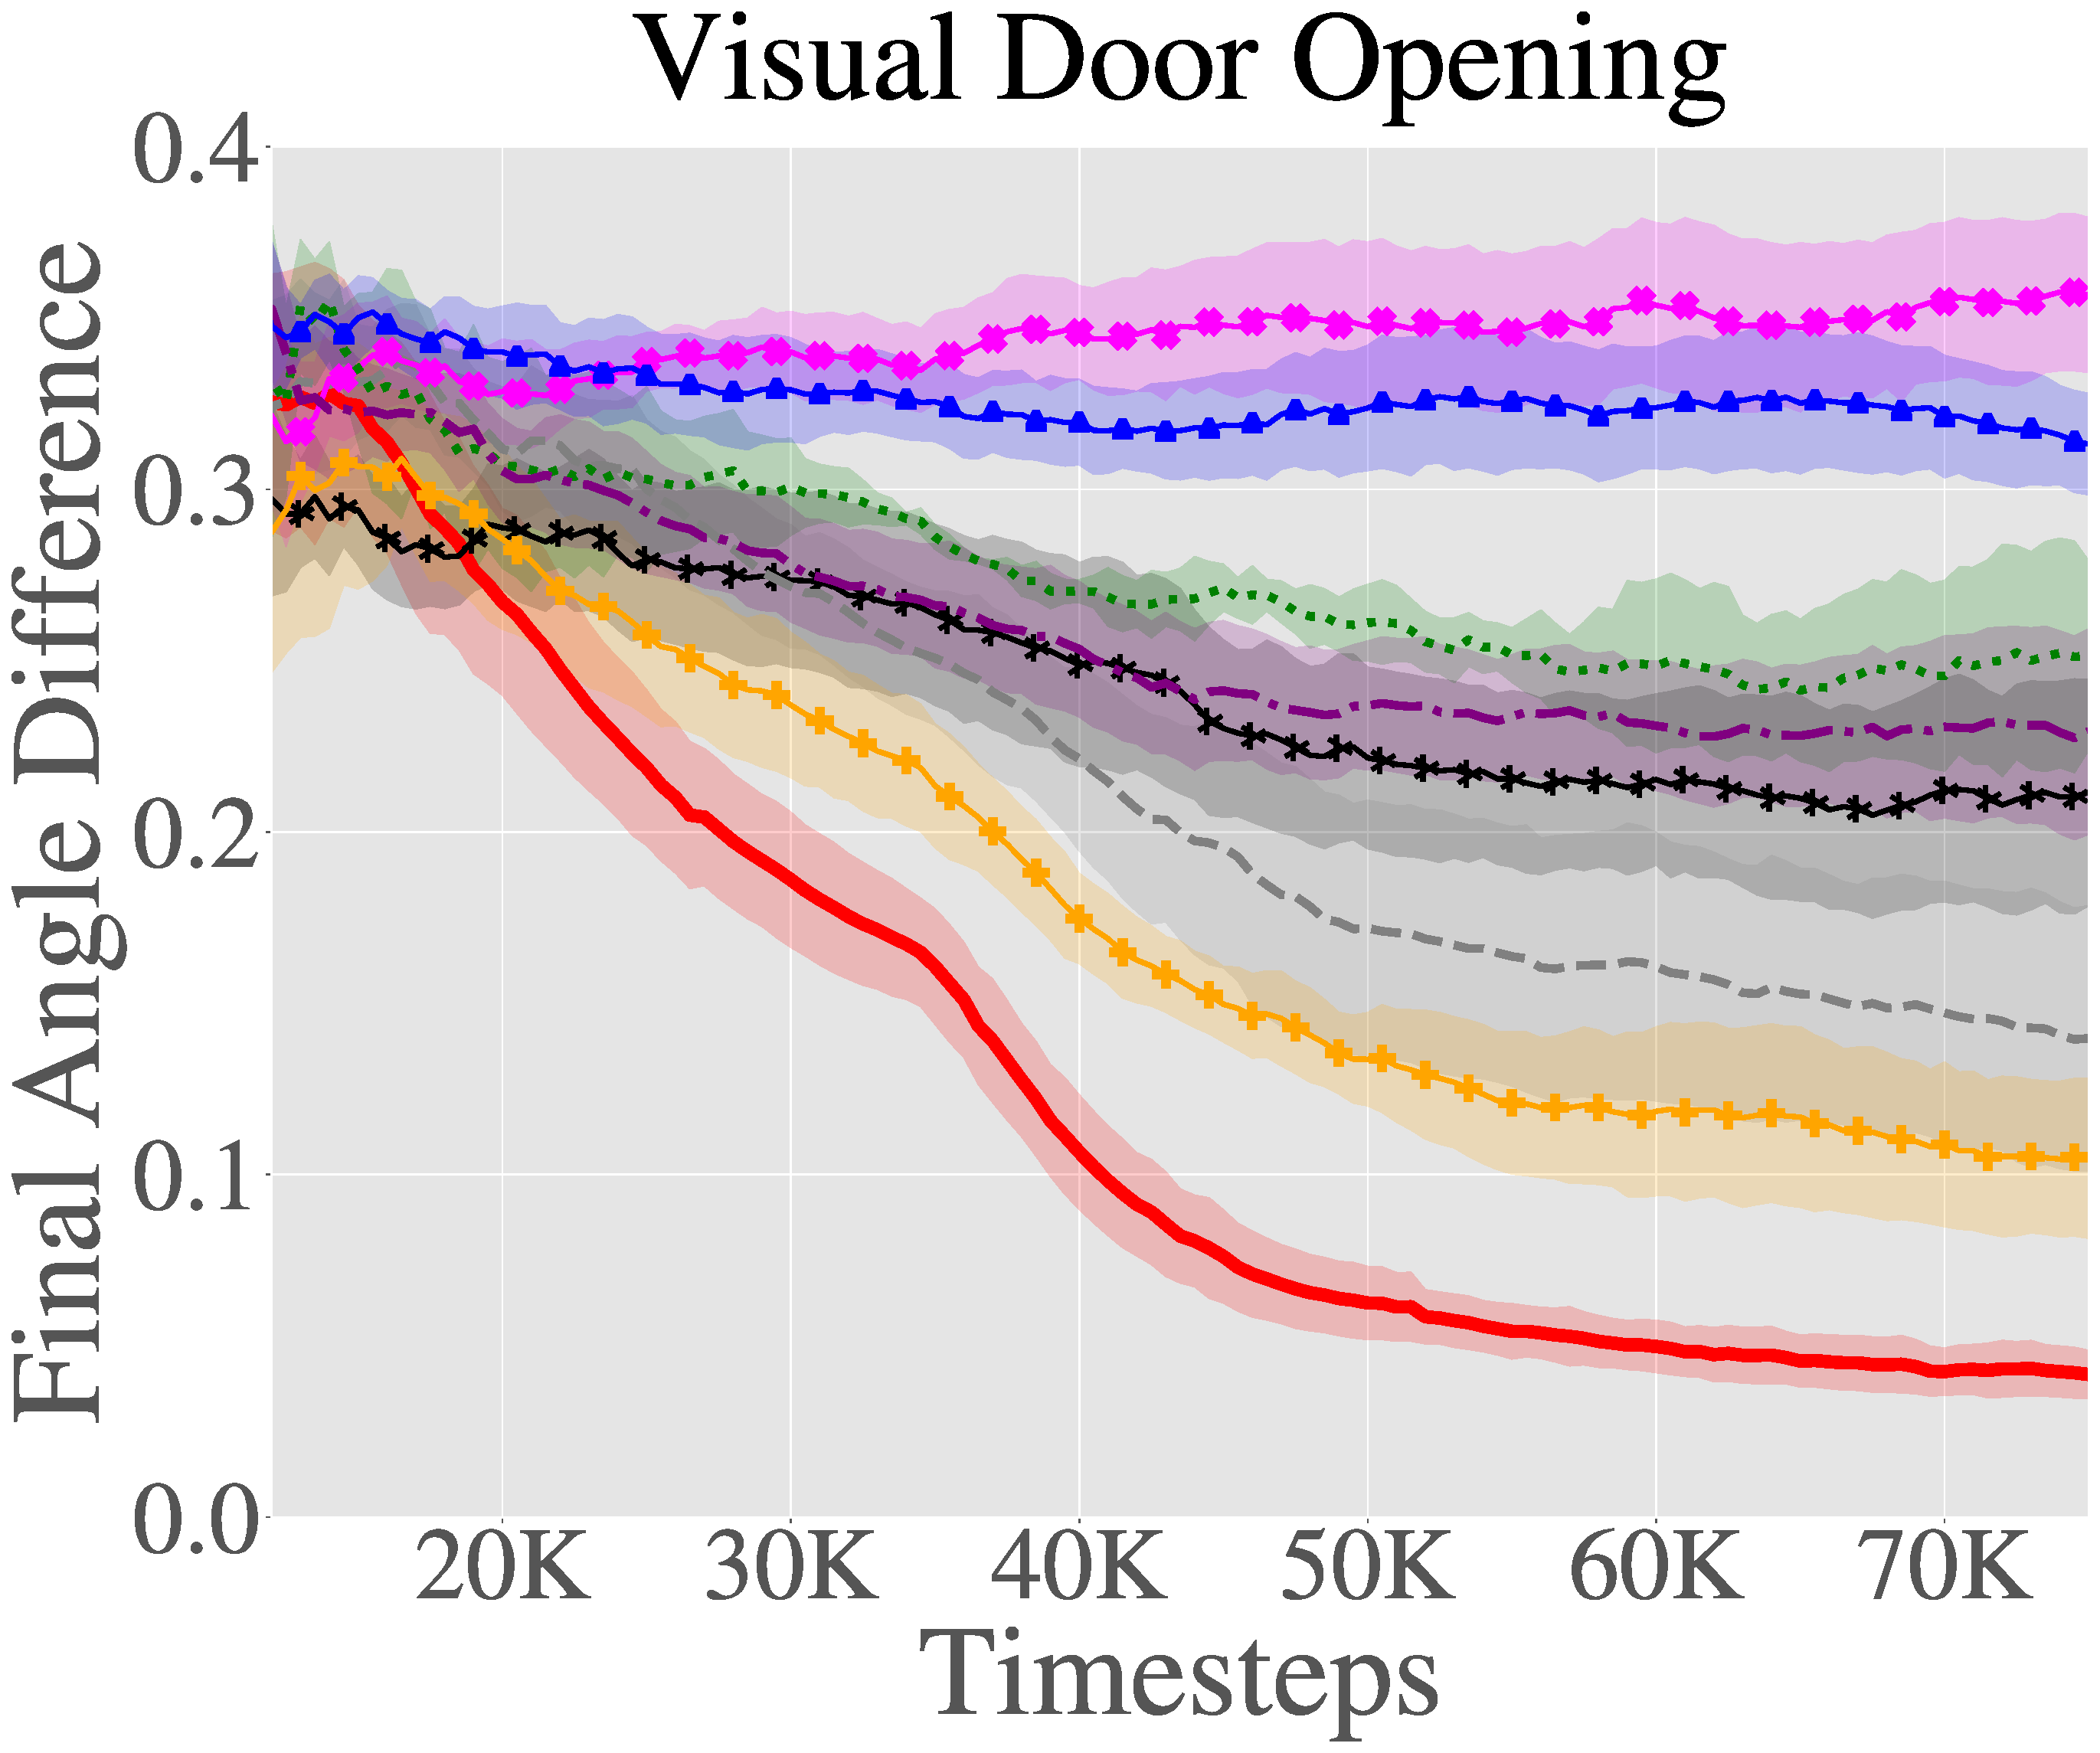
\includegraphics[width=\linewidth]{skewfit/figures/plots/main_sim_fig/door_big.pdf}
          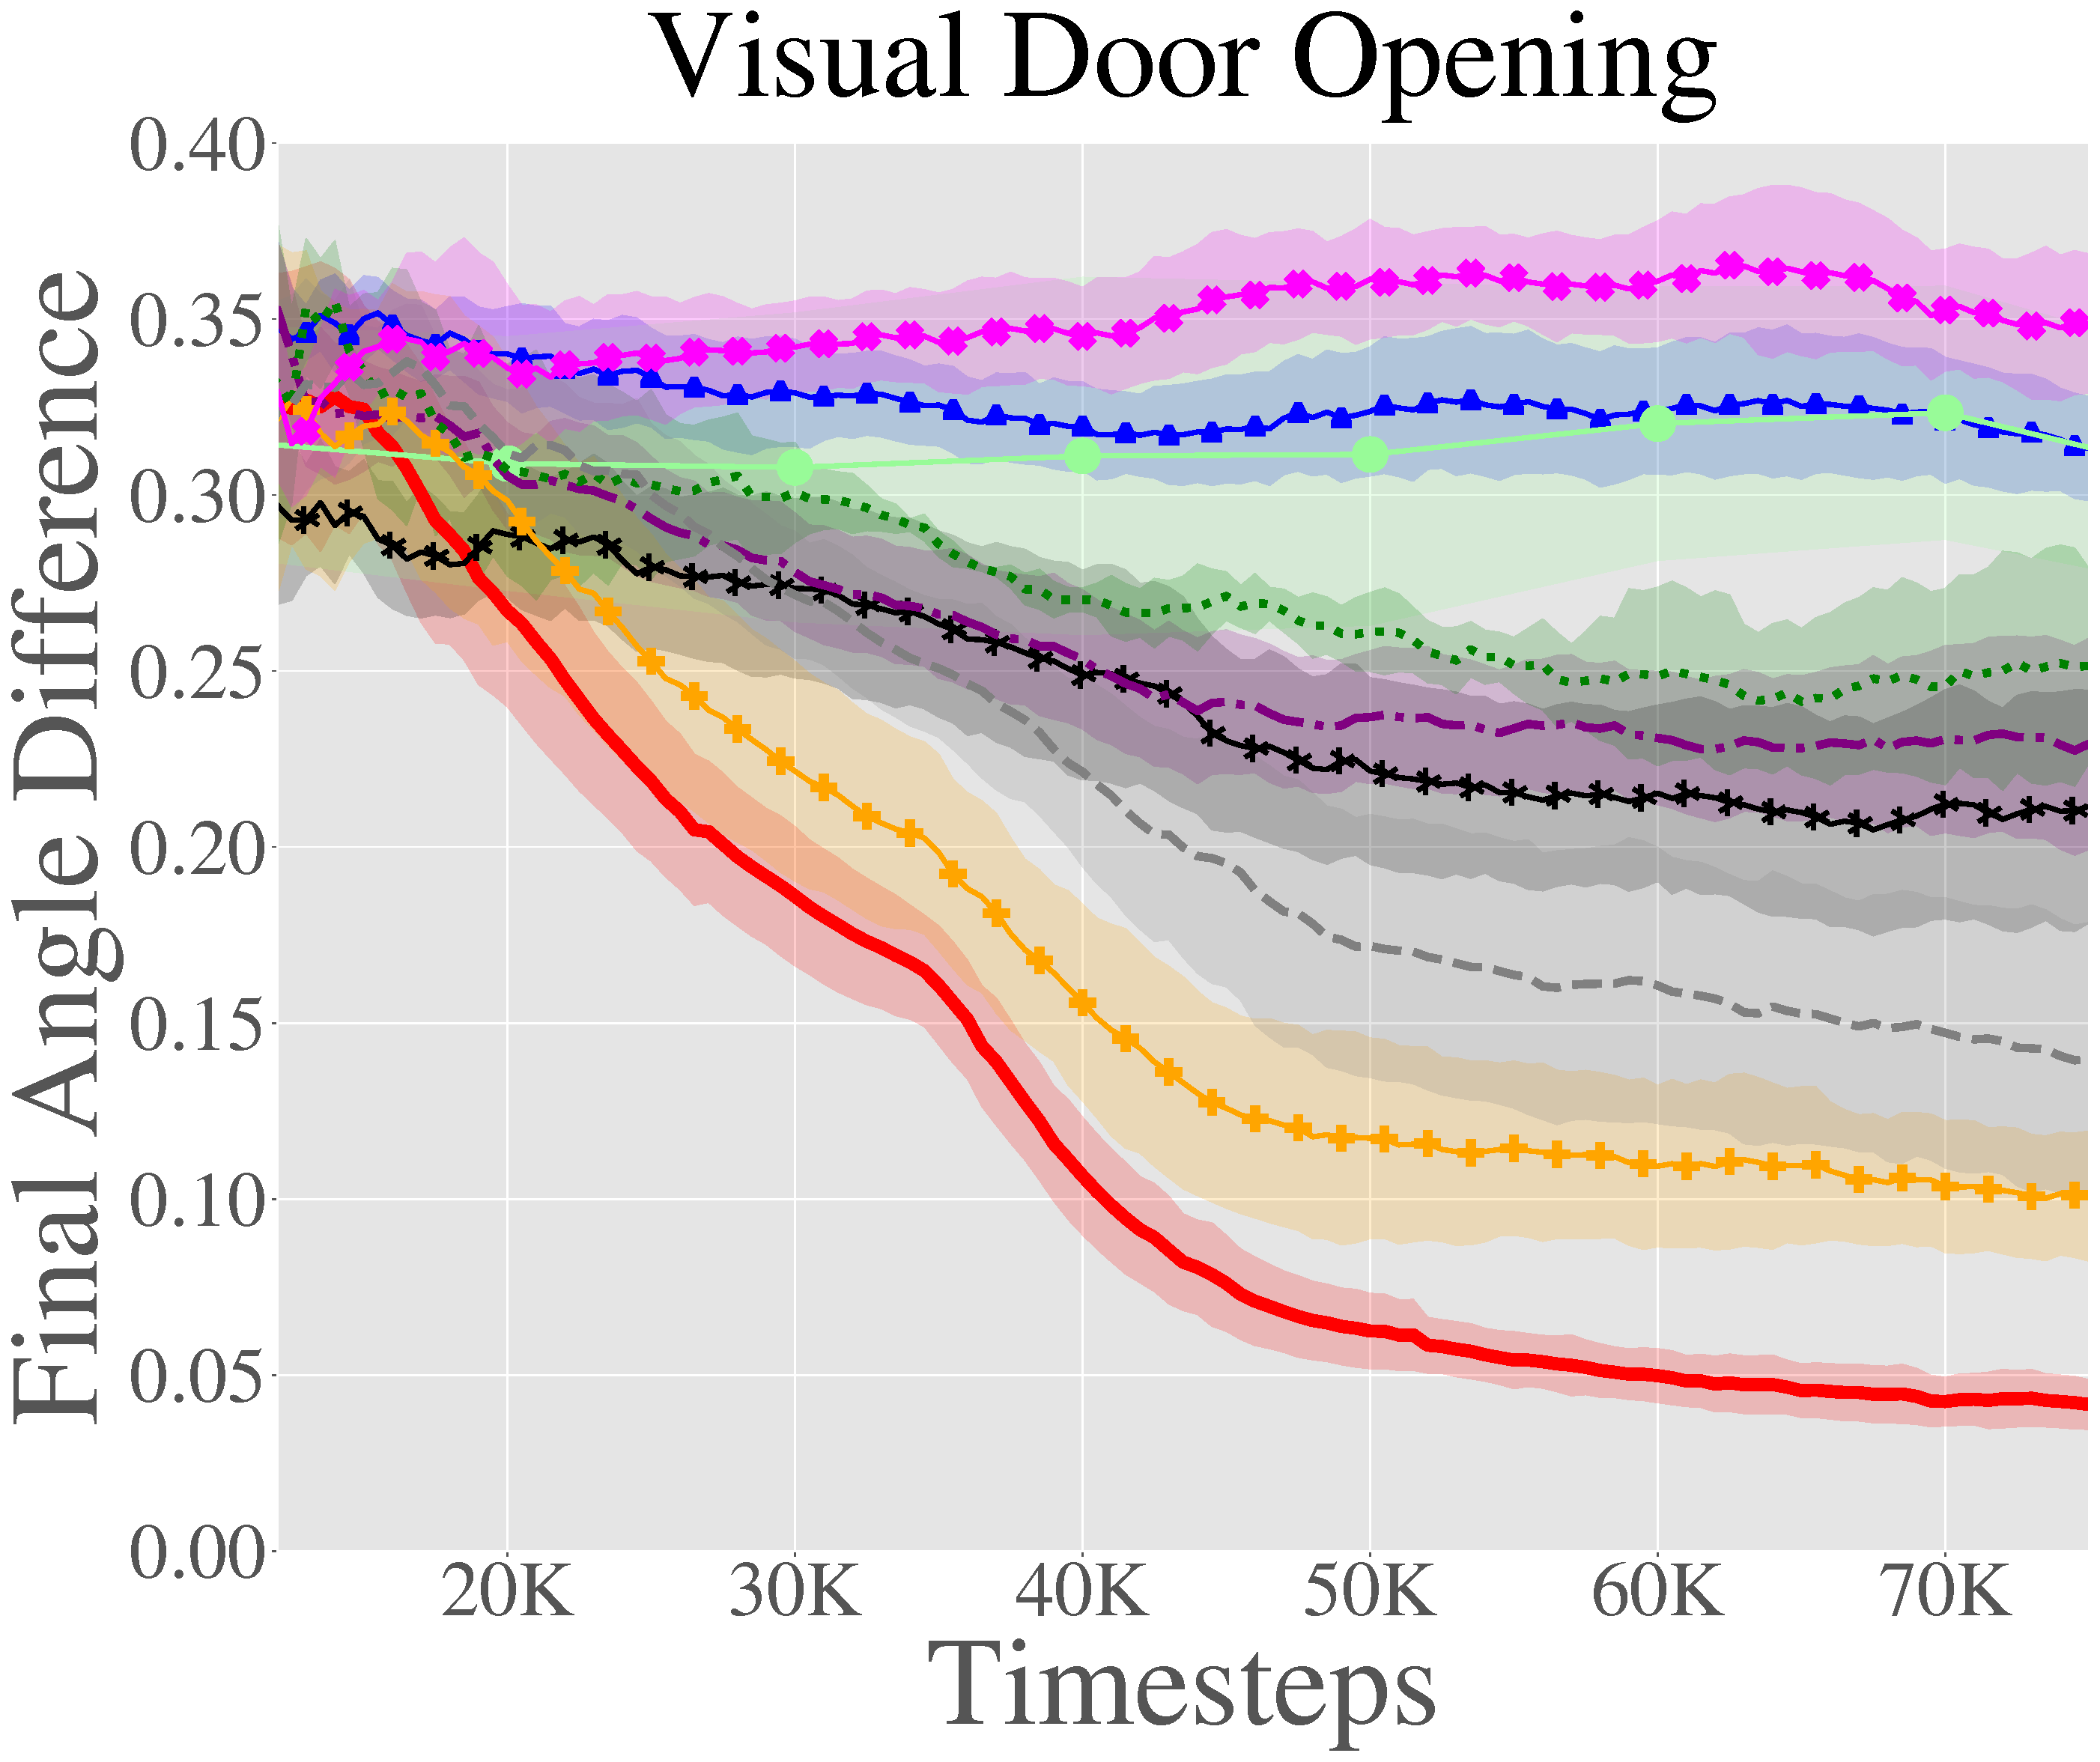
\includegraphics[width=\linewidth]{skewfit/figures/plots/main_sawyer_fig_with_hazan/door.pdf}
  \end{subfigure}
  \hfill
  \begin{subfigure}[t]{.49\linewidth}
    \centering
        % 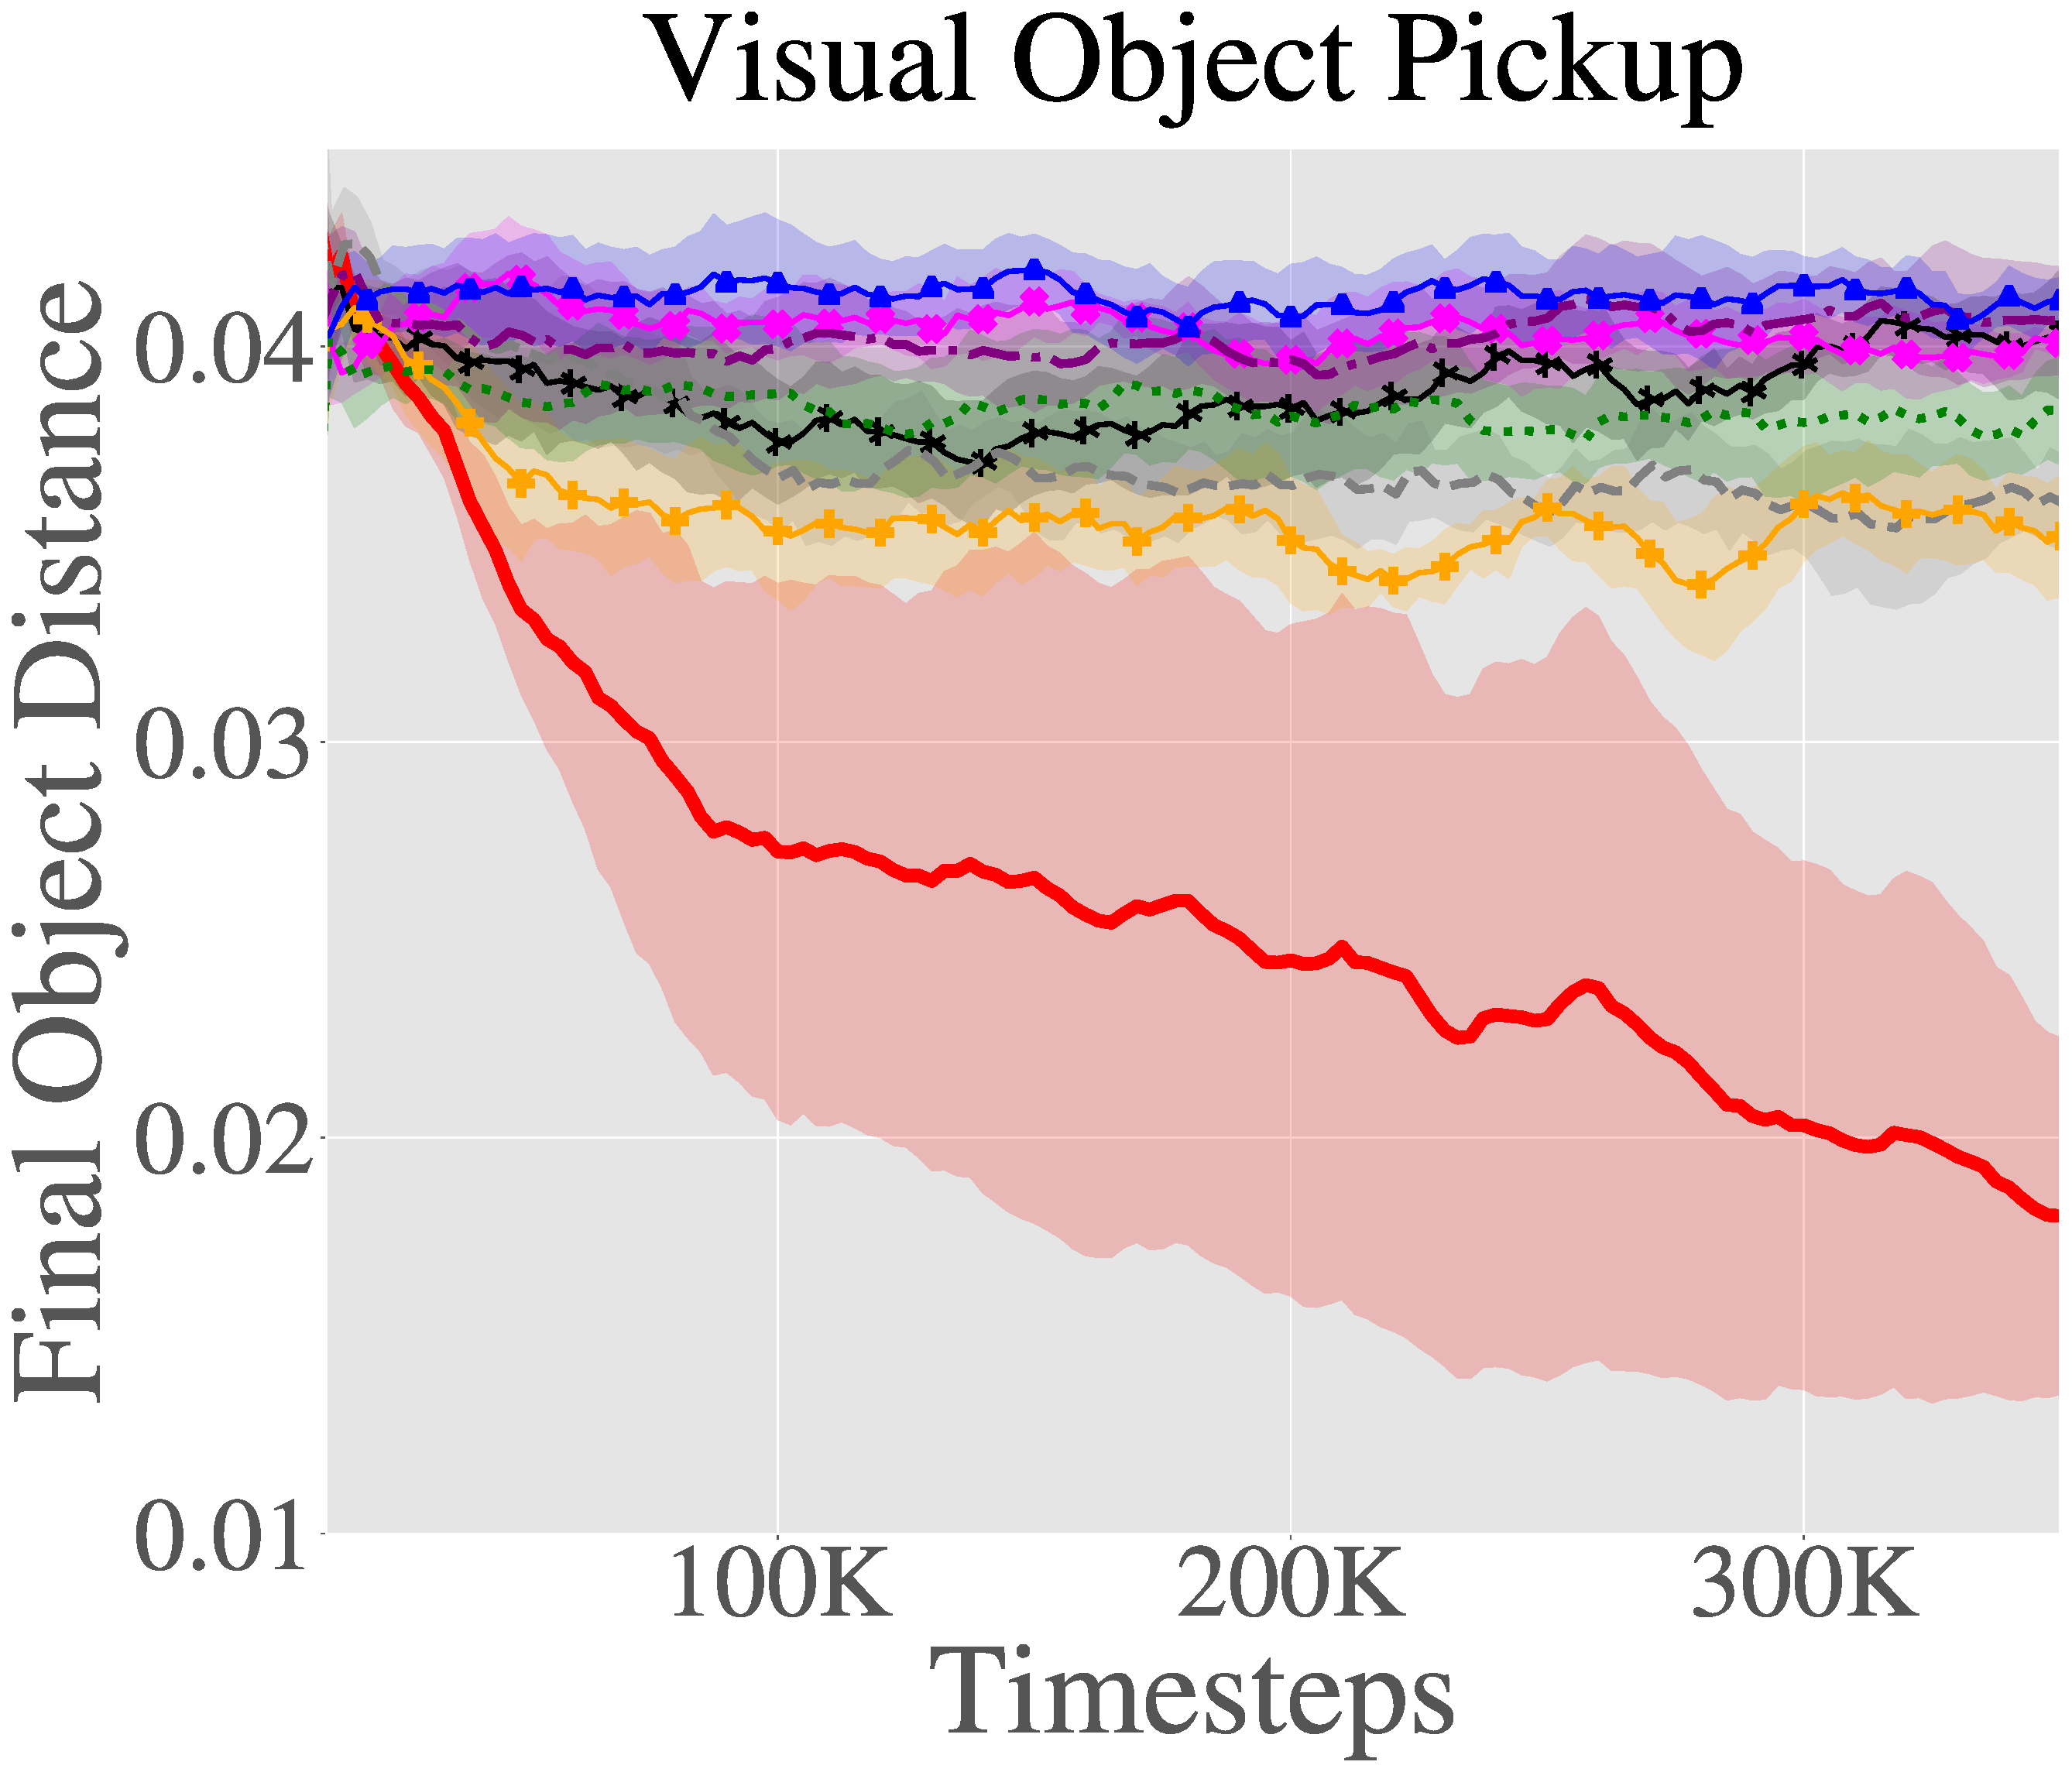
\includegraphics[width=\linewidth]{skewfit/figures/plots/main_sim_fig/pickup_big.pdf}
          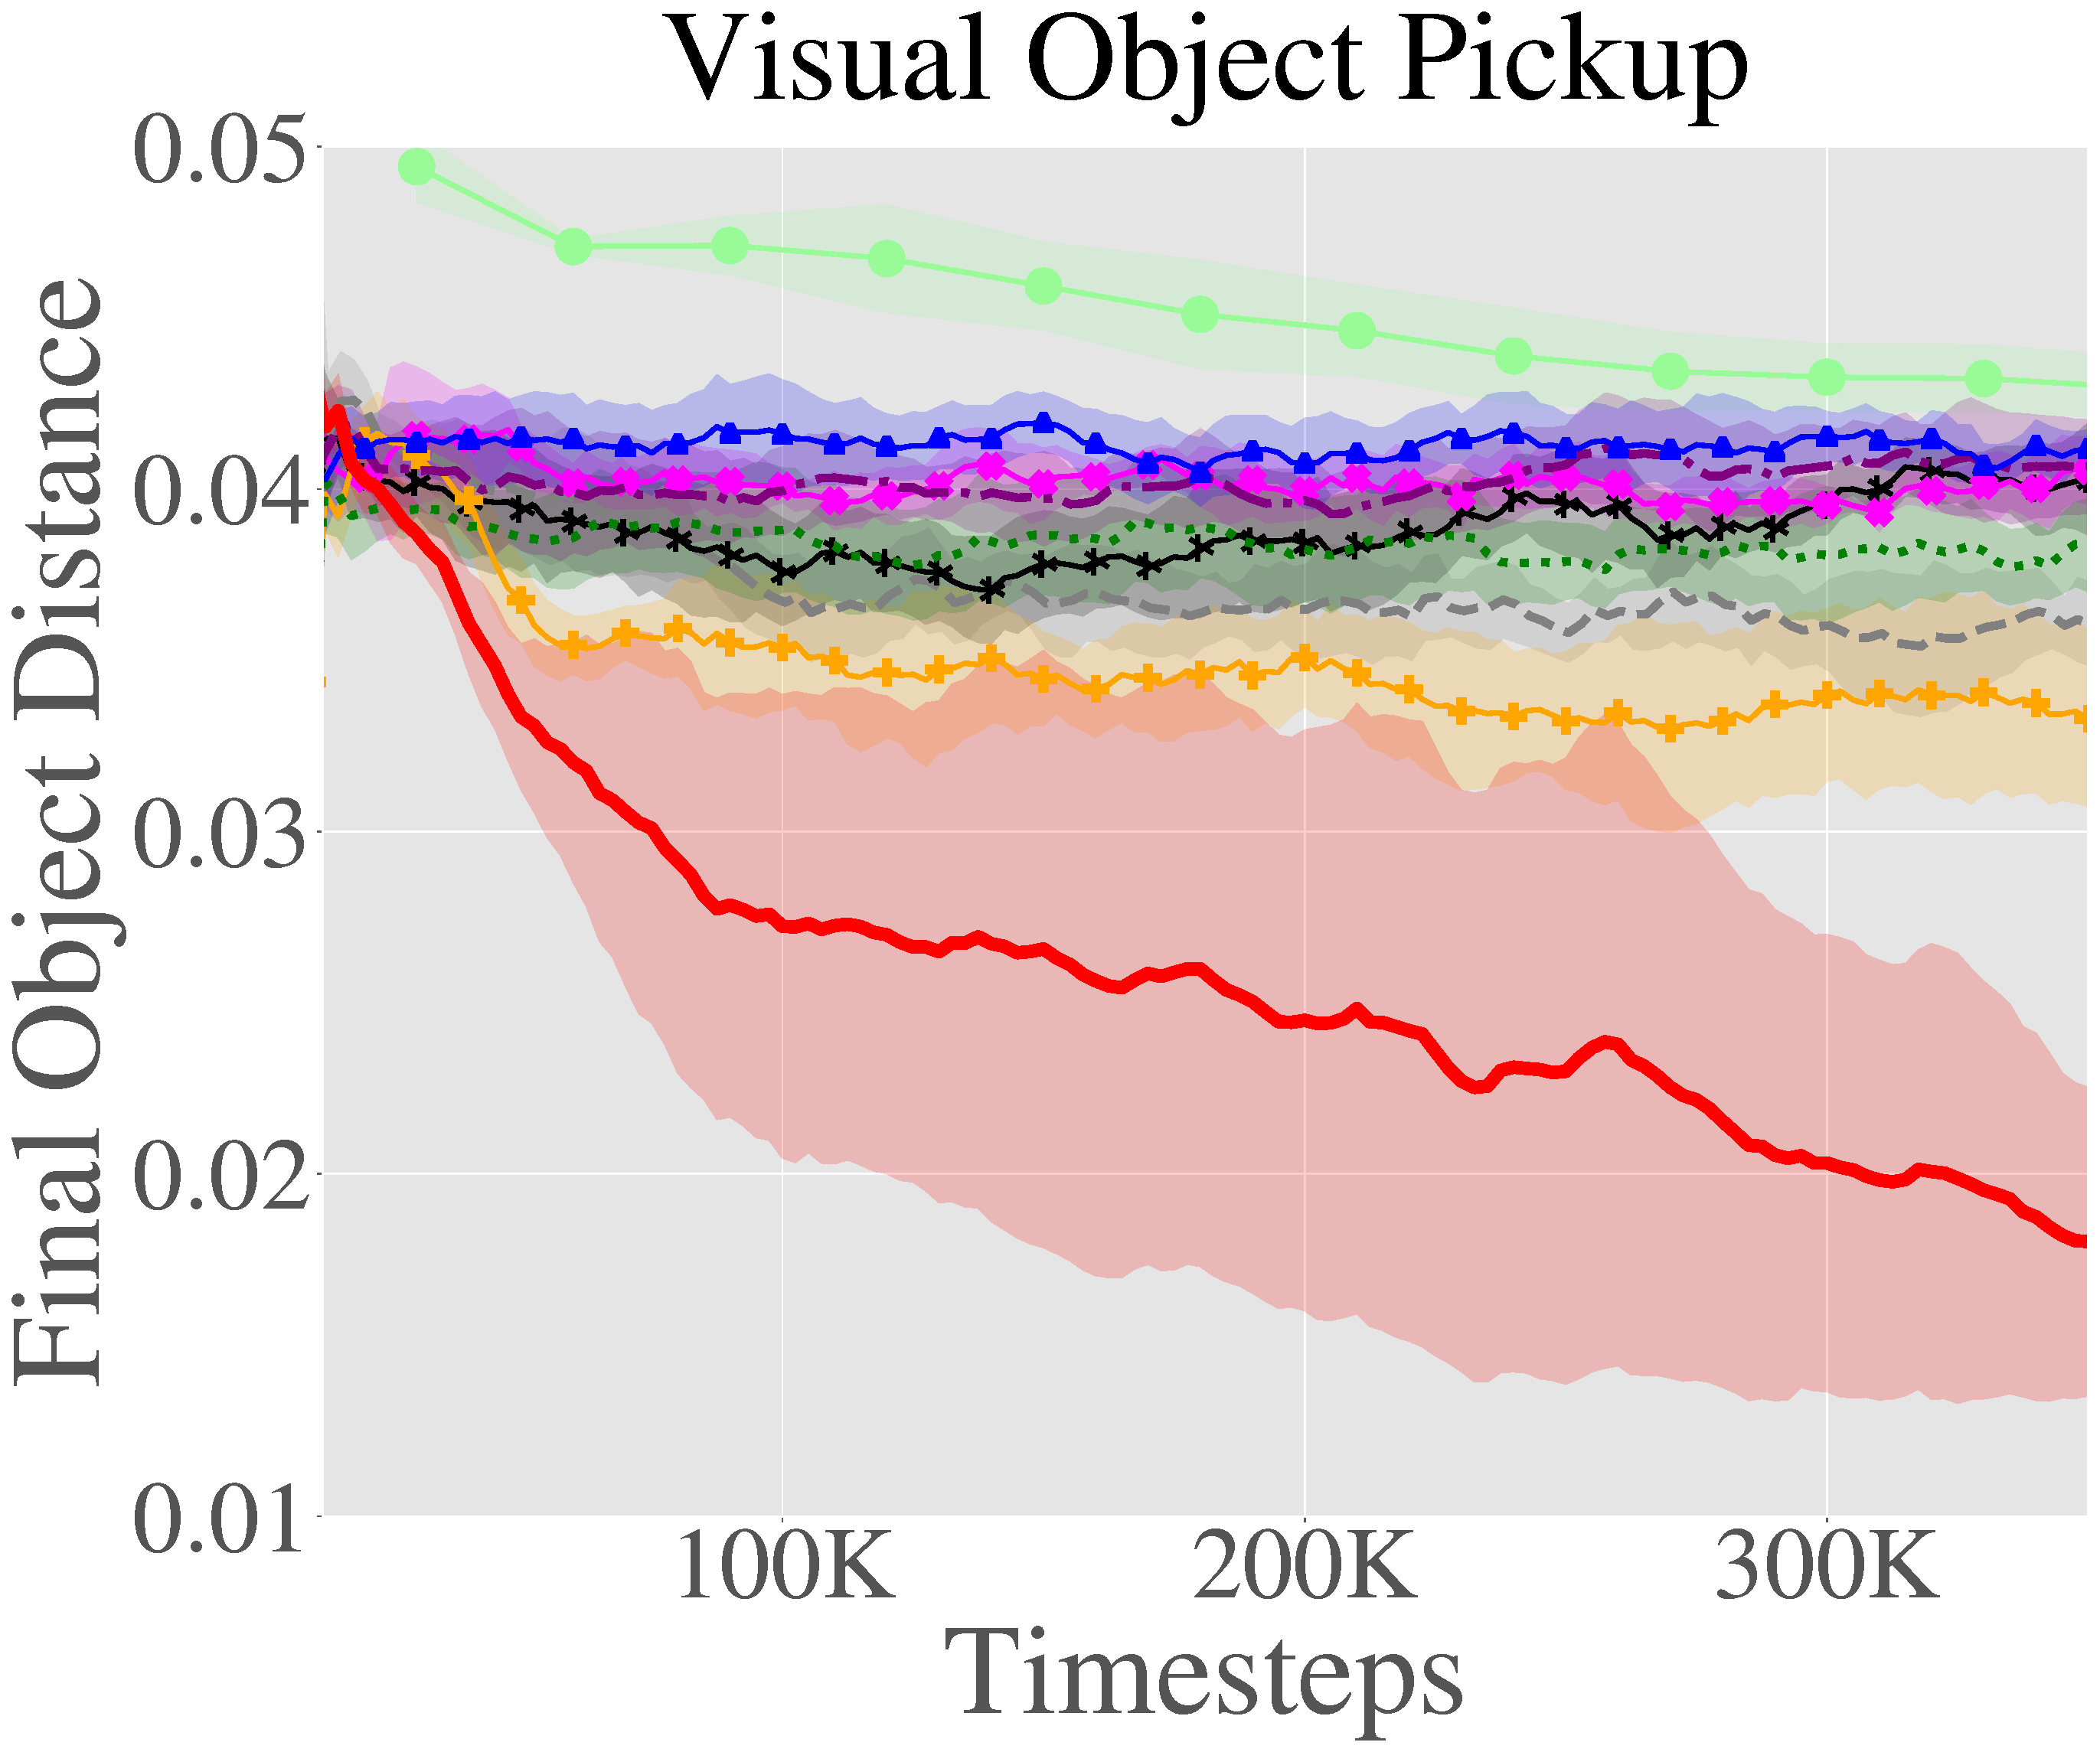
\includegraphics[width=\linewidth]{skewfit/figures/plots/main_sawyer_fig_with_hazan/pickup.pdf}
  \end{subfigure}

  \medskip

  \begin{subfigure}[t]{.49\linewidth}
    \centering
        %   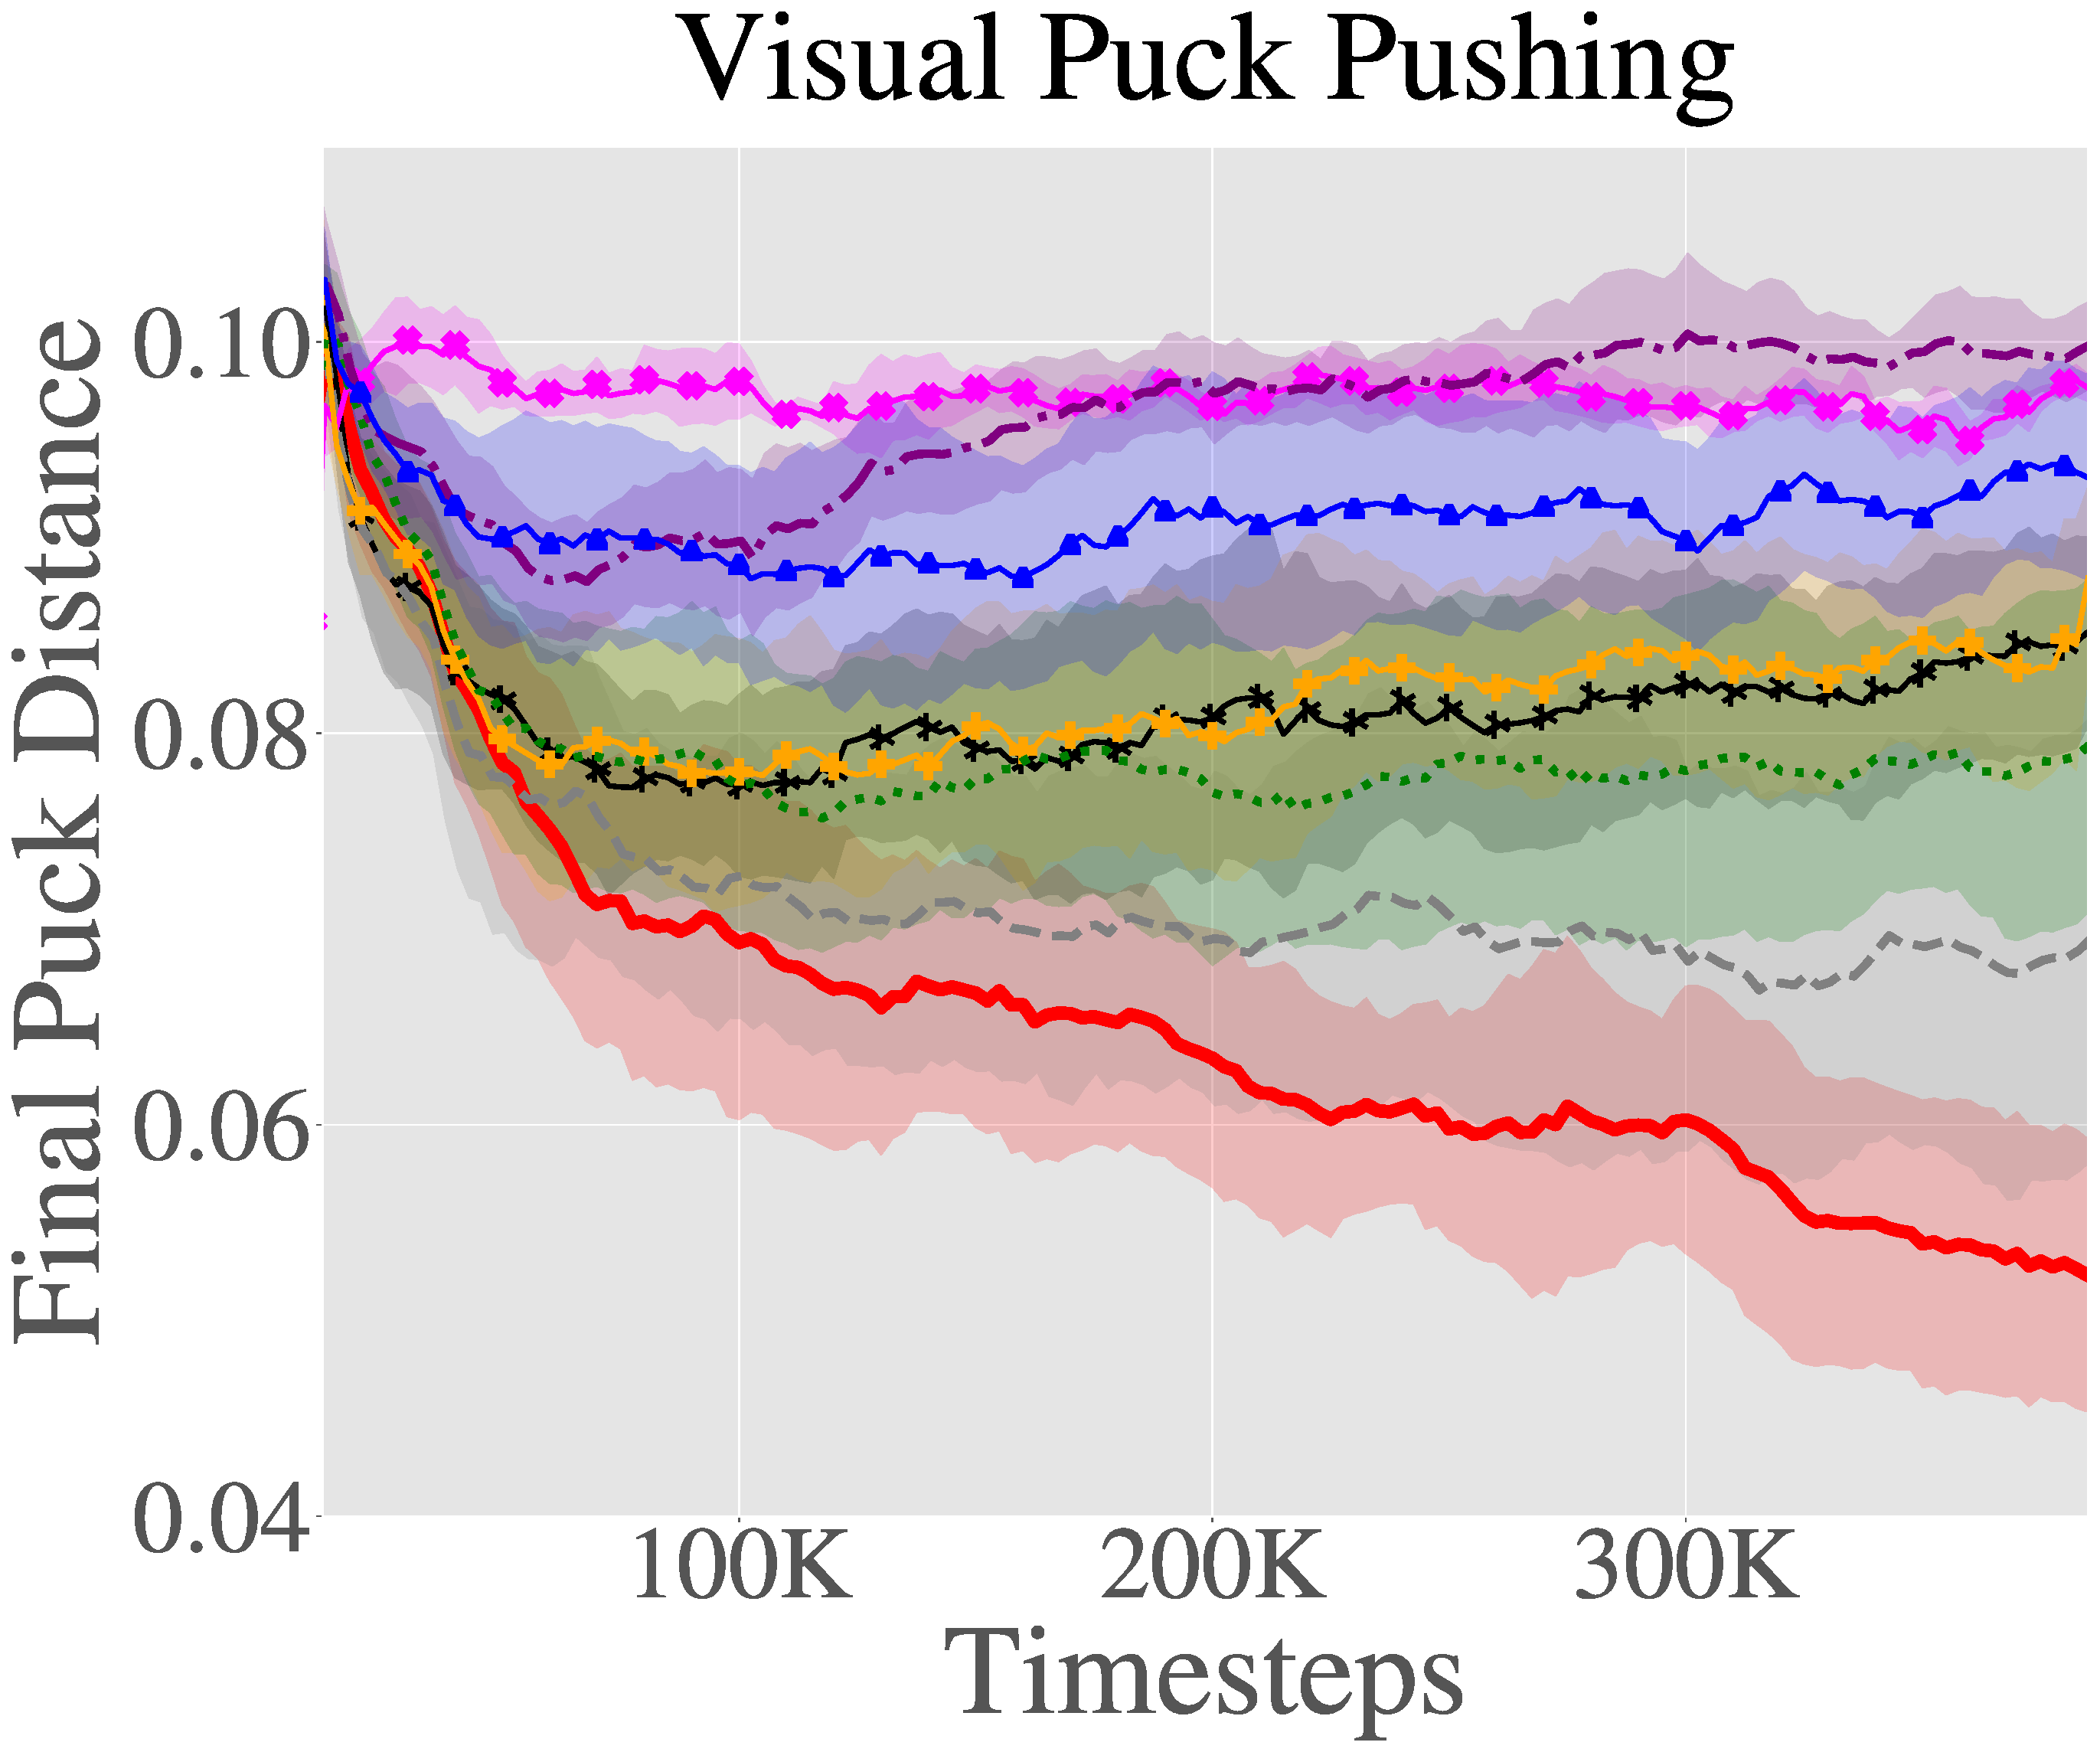
\includegraphics[width=\linewidth]{skewfit/figures/plots/main_sim_fig/pusher_big.pdf}
          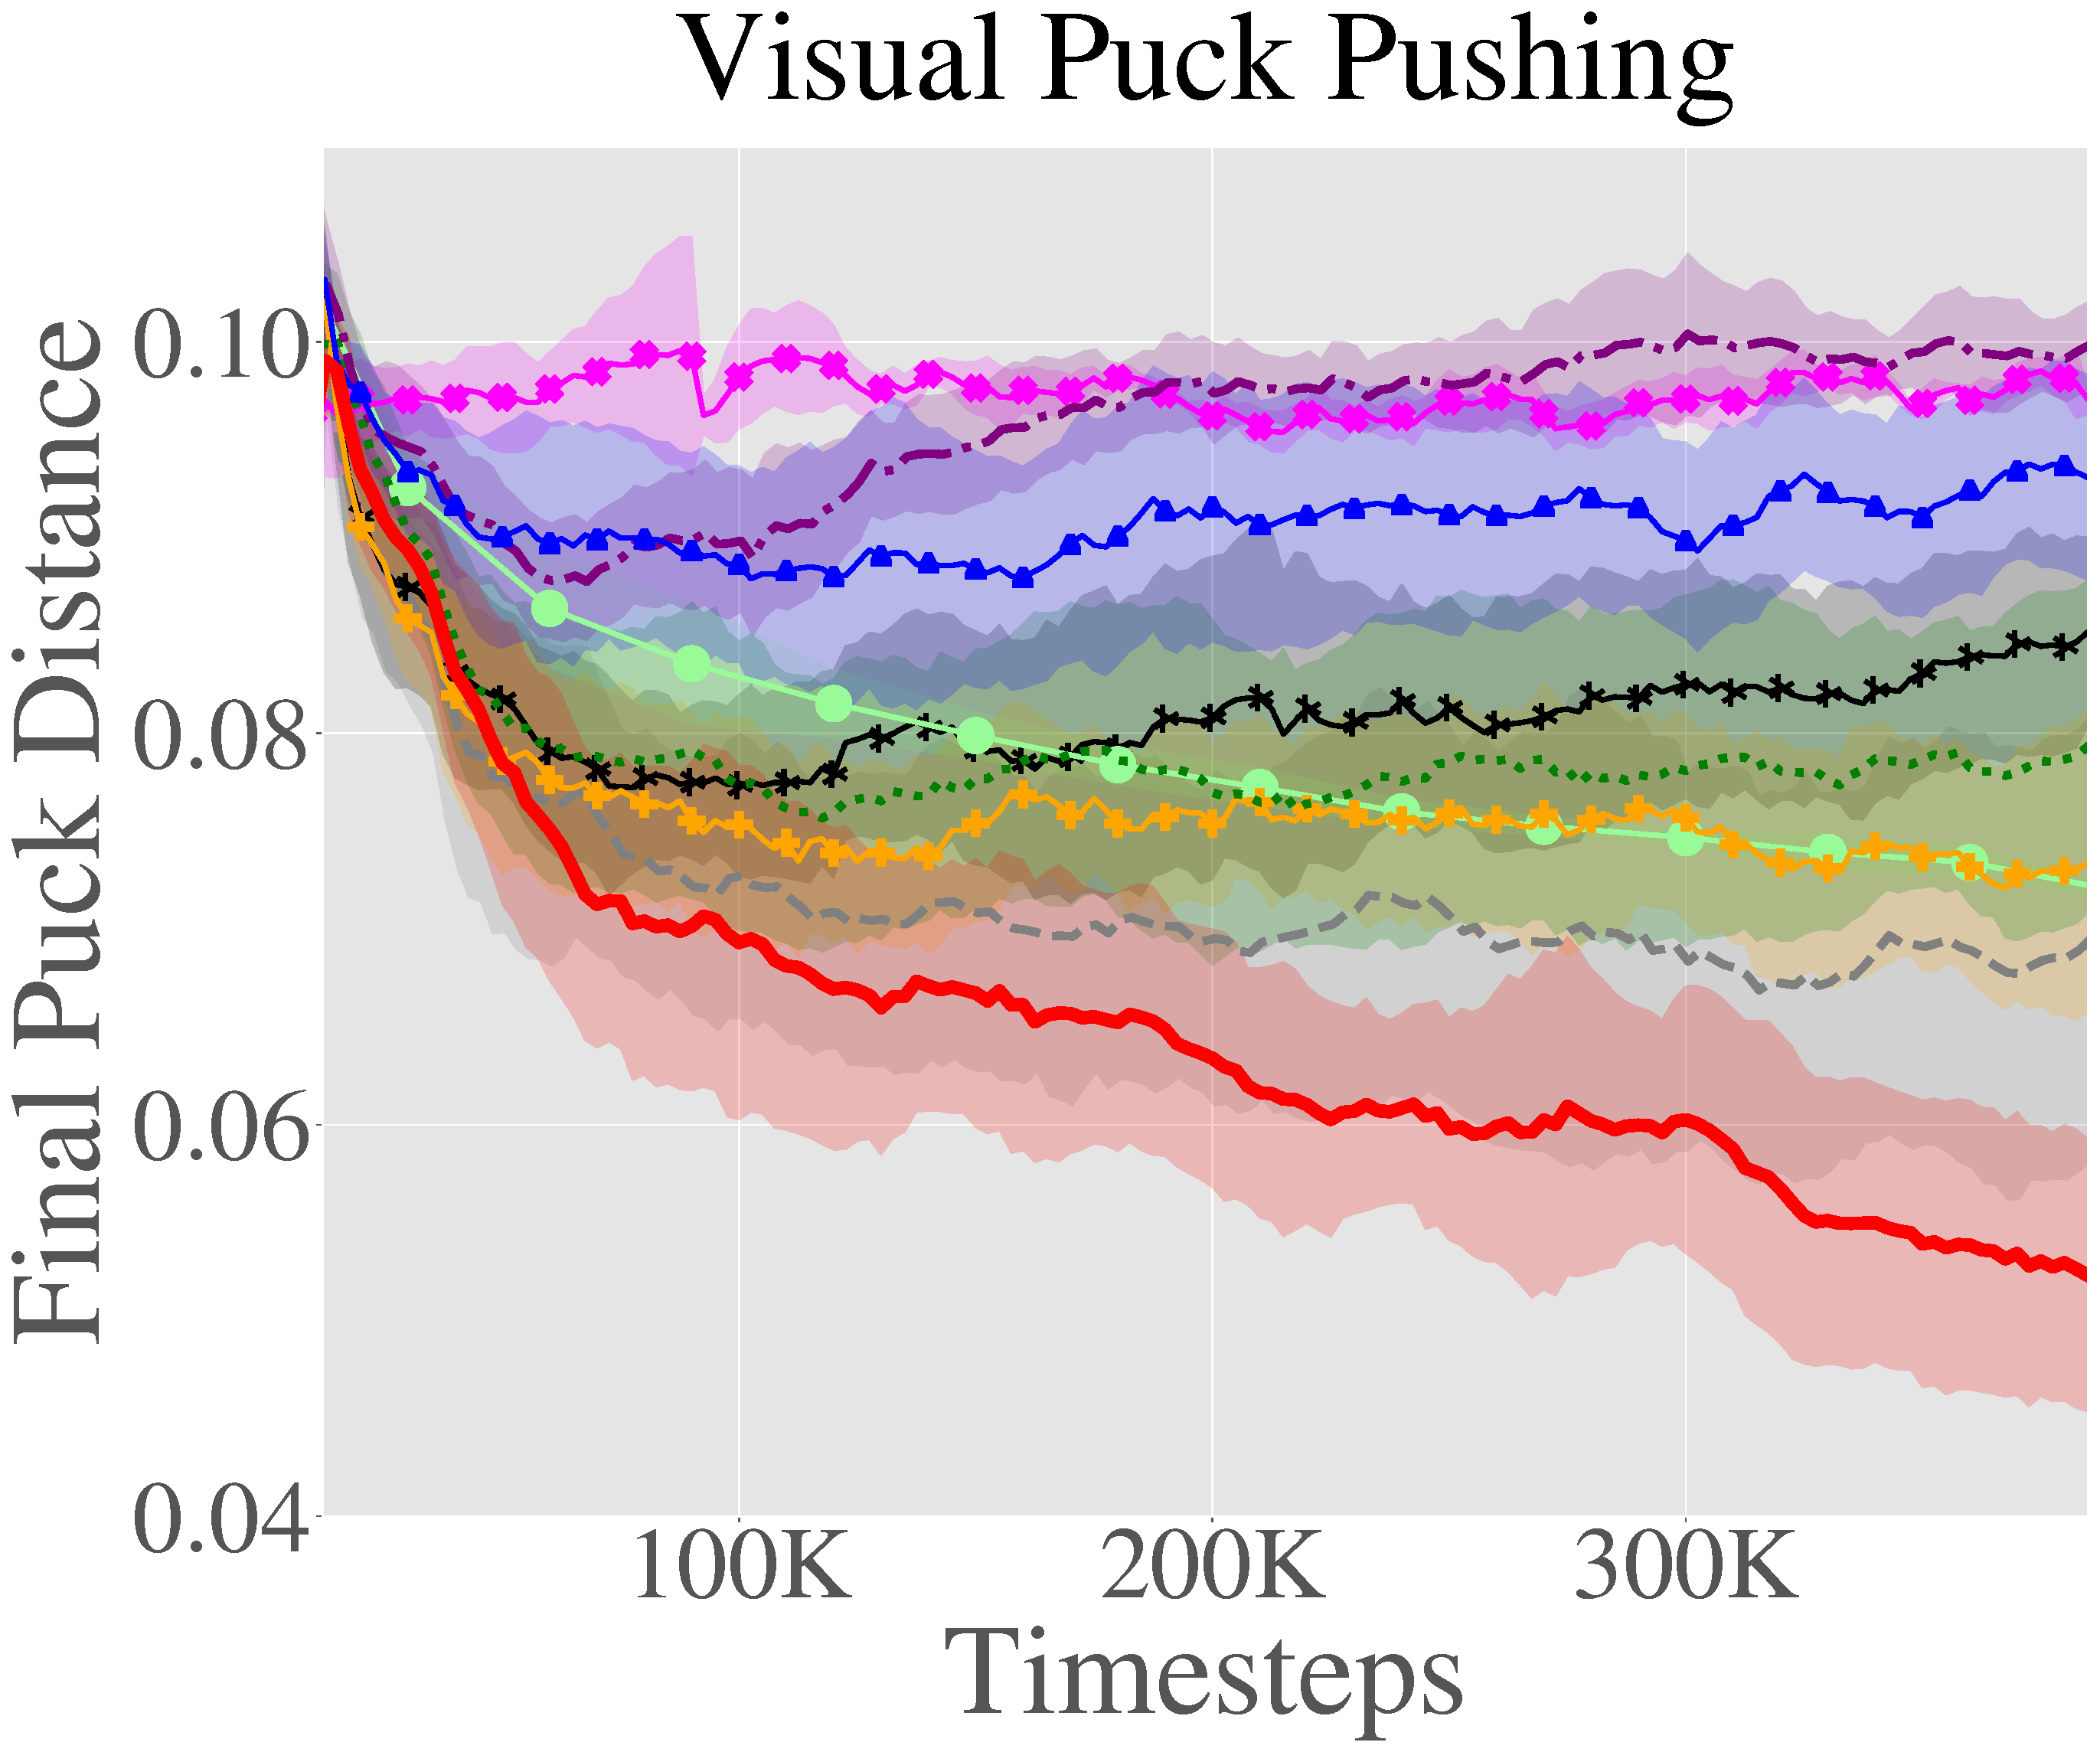
\includegraphics[width=\linewidth]{skewfit/figures/plots/main_sawyer_fig_with_hazan/pusher.pdf}
  \end{subfigure}
  \hfill
  \begin{subfigure}[t]{.48\linewidth}
    \centering
    % \hspace{0.165in}
    \raisebox{0.16in}{
        % 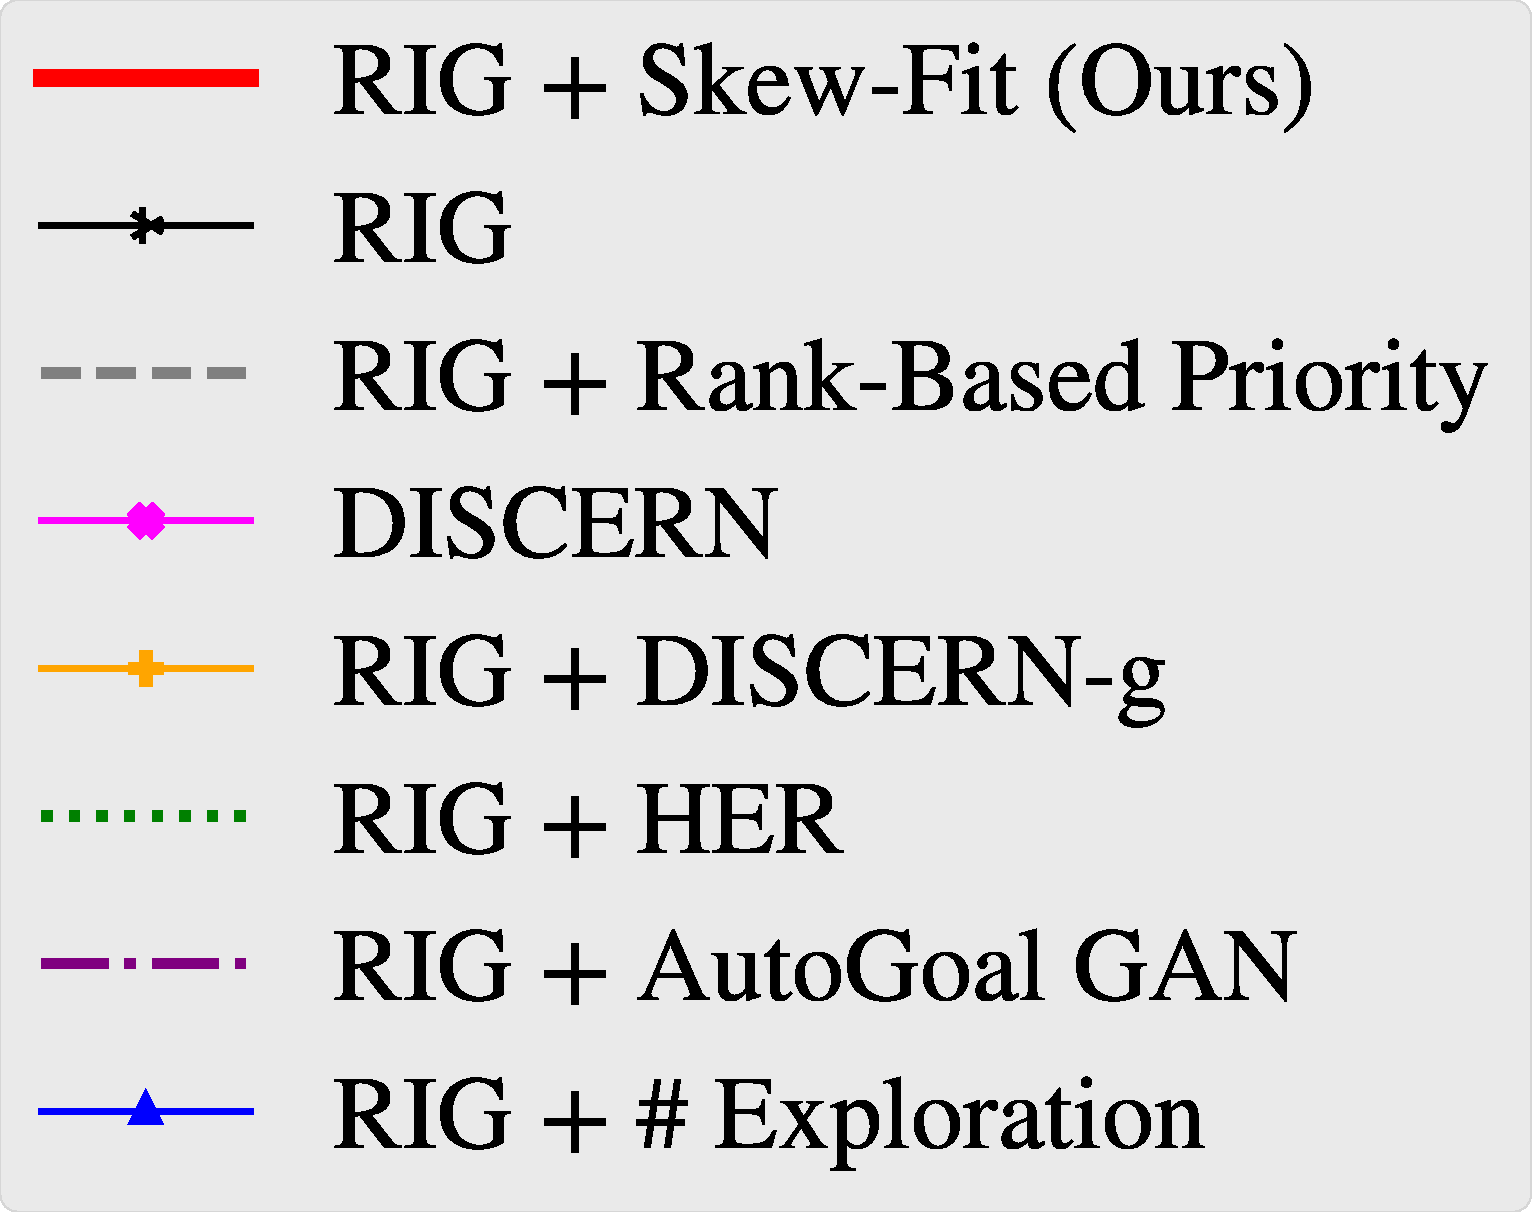
\includegraphics[width=0.8\linewidth]{skewfit/figures/plots/main_sim_fig/legend.pdf}
          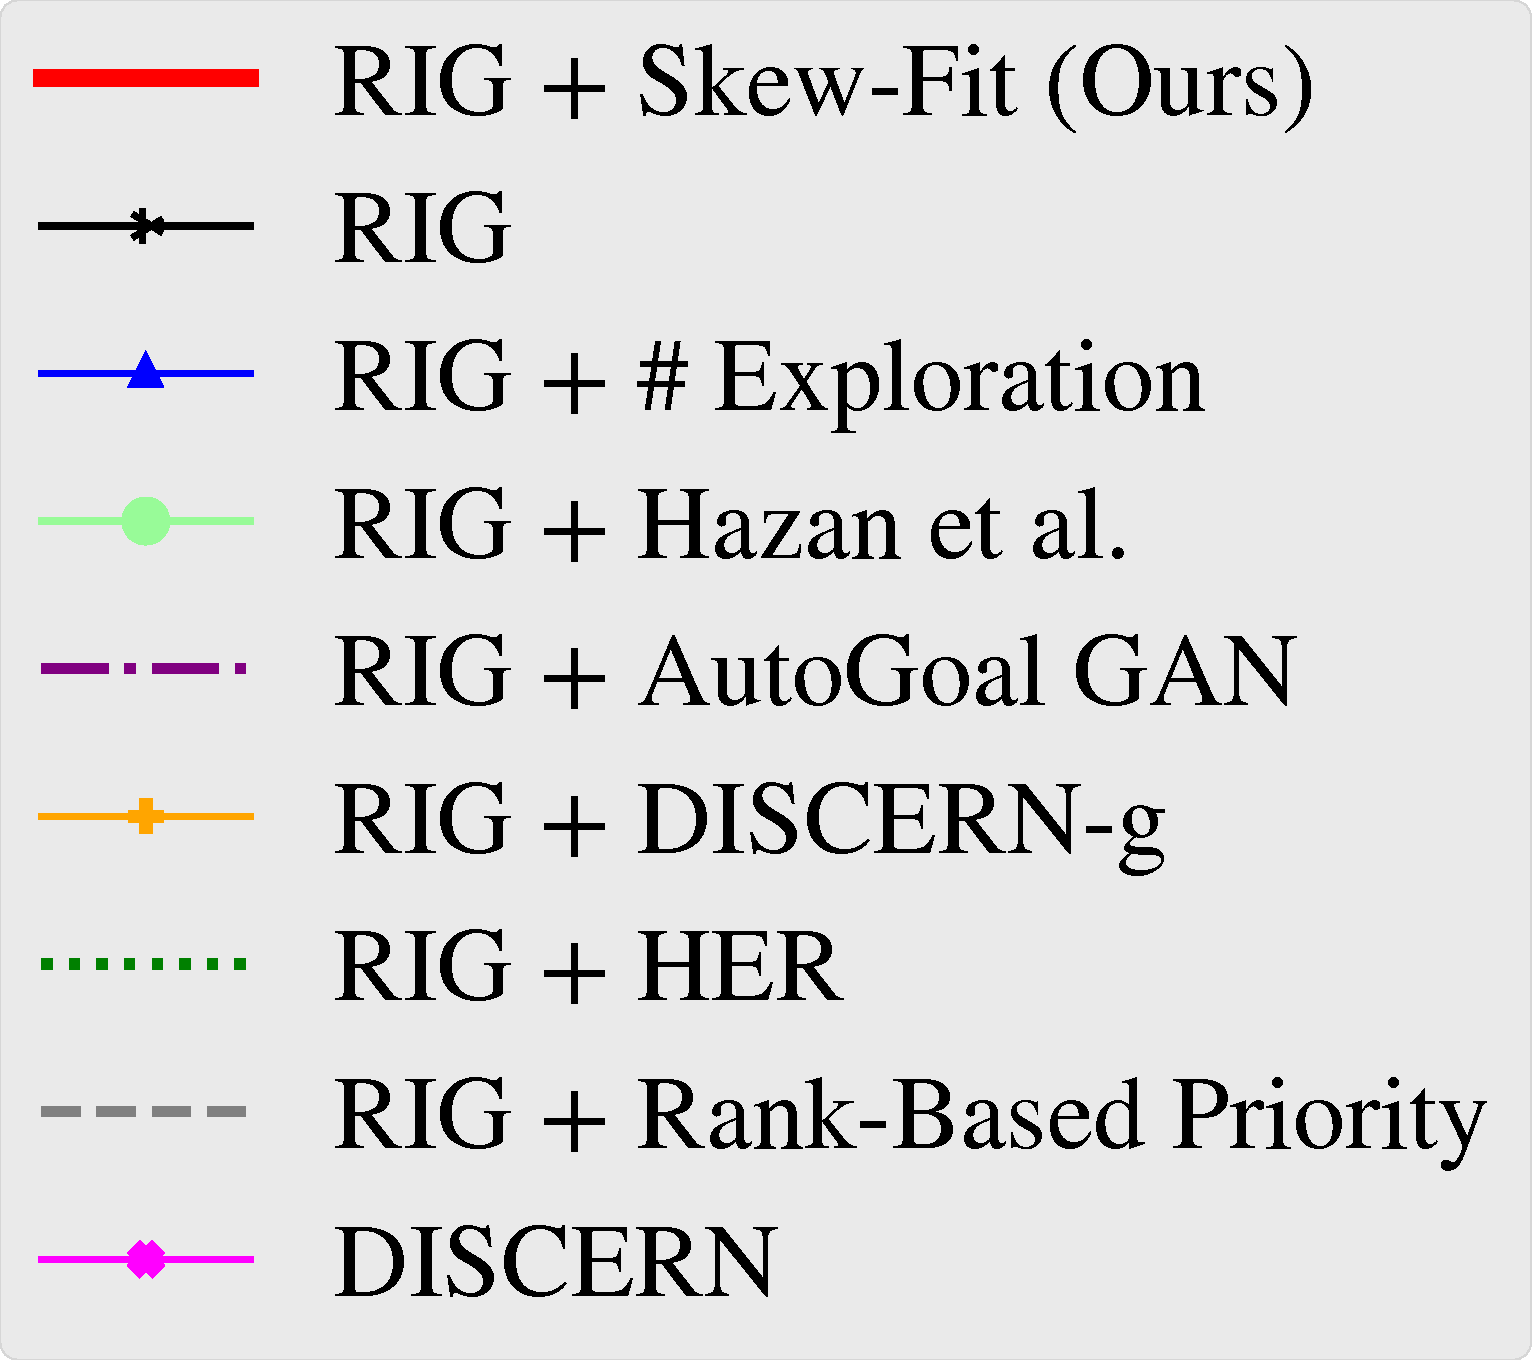
\includegraphics[width=\linewidth]{skewfit/figures/plots/main_sawyer_fig_with_hazan/main_figure_legend_with_hazan.pdf}
    }
  \end{subfigure}
    \fcaption{
        Learning curves for simulated continuous control tasks.
        Lower is better.
        We show the mean and standard deviation of 6 seeds and smooth temporally across 50 epochs within each seed.
        \METHOD consistently outperforms RIG and various prior methods.
        See text for description of each method.
    }
    \label{fig:sim-results}
\end{figure}


We see in \Figref{fig:sim-results} that Skew-Fit significantly outperforms prior methods both in terms of task performance and sample complexity.
The most common failure mode for prior methods is that the goal distributions collapse, resulting in the agent learning to reach only a fraction of the state space, as shown in \autoref{fig:offline-sk-real}.
For comparison, additional samples of $\pg$ when trained with and without \METHOD are shown in \autoref{sec:vae-dump}.
Those images show that without \METHOD, $\pg$ produces a small, non-diverse distribution for each environment: the object is in the same place for pickup, the puck is often in the starting position for pushing, and the door is always closed.
In contrast, \METHOD proposes goals where the object is in the air and on the ground, where the puck positions are varied, and the door angle changes.

We can see the effect of these goal choices by visualizing more example rollouts for RIG and \METHOD.
These visuals, shown in \Figref{fig:example_rollouts} in \autoref{sec:vae-dump}, show that RIG only learns to reach states close to the initial position, while \METHOD learns to reach the entire state space.
For a quantitative comparison, \Figref{fig:exploration_pickups} shows the cumulative total exploration pickups for each method.
From the graph, we see that many methods have a near-constant rate of object lifts throughout all of training.
\METHOD is the only method that significantly increases the rate at which the policy picks up the object during exploration, suggesting that only \METHOD sets goals that encourage the policy to interact with the object.

\begin{figure}[t]
\centering
  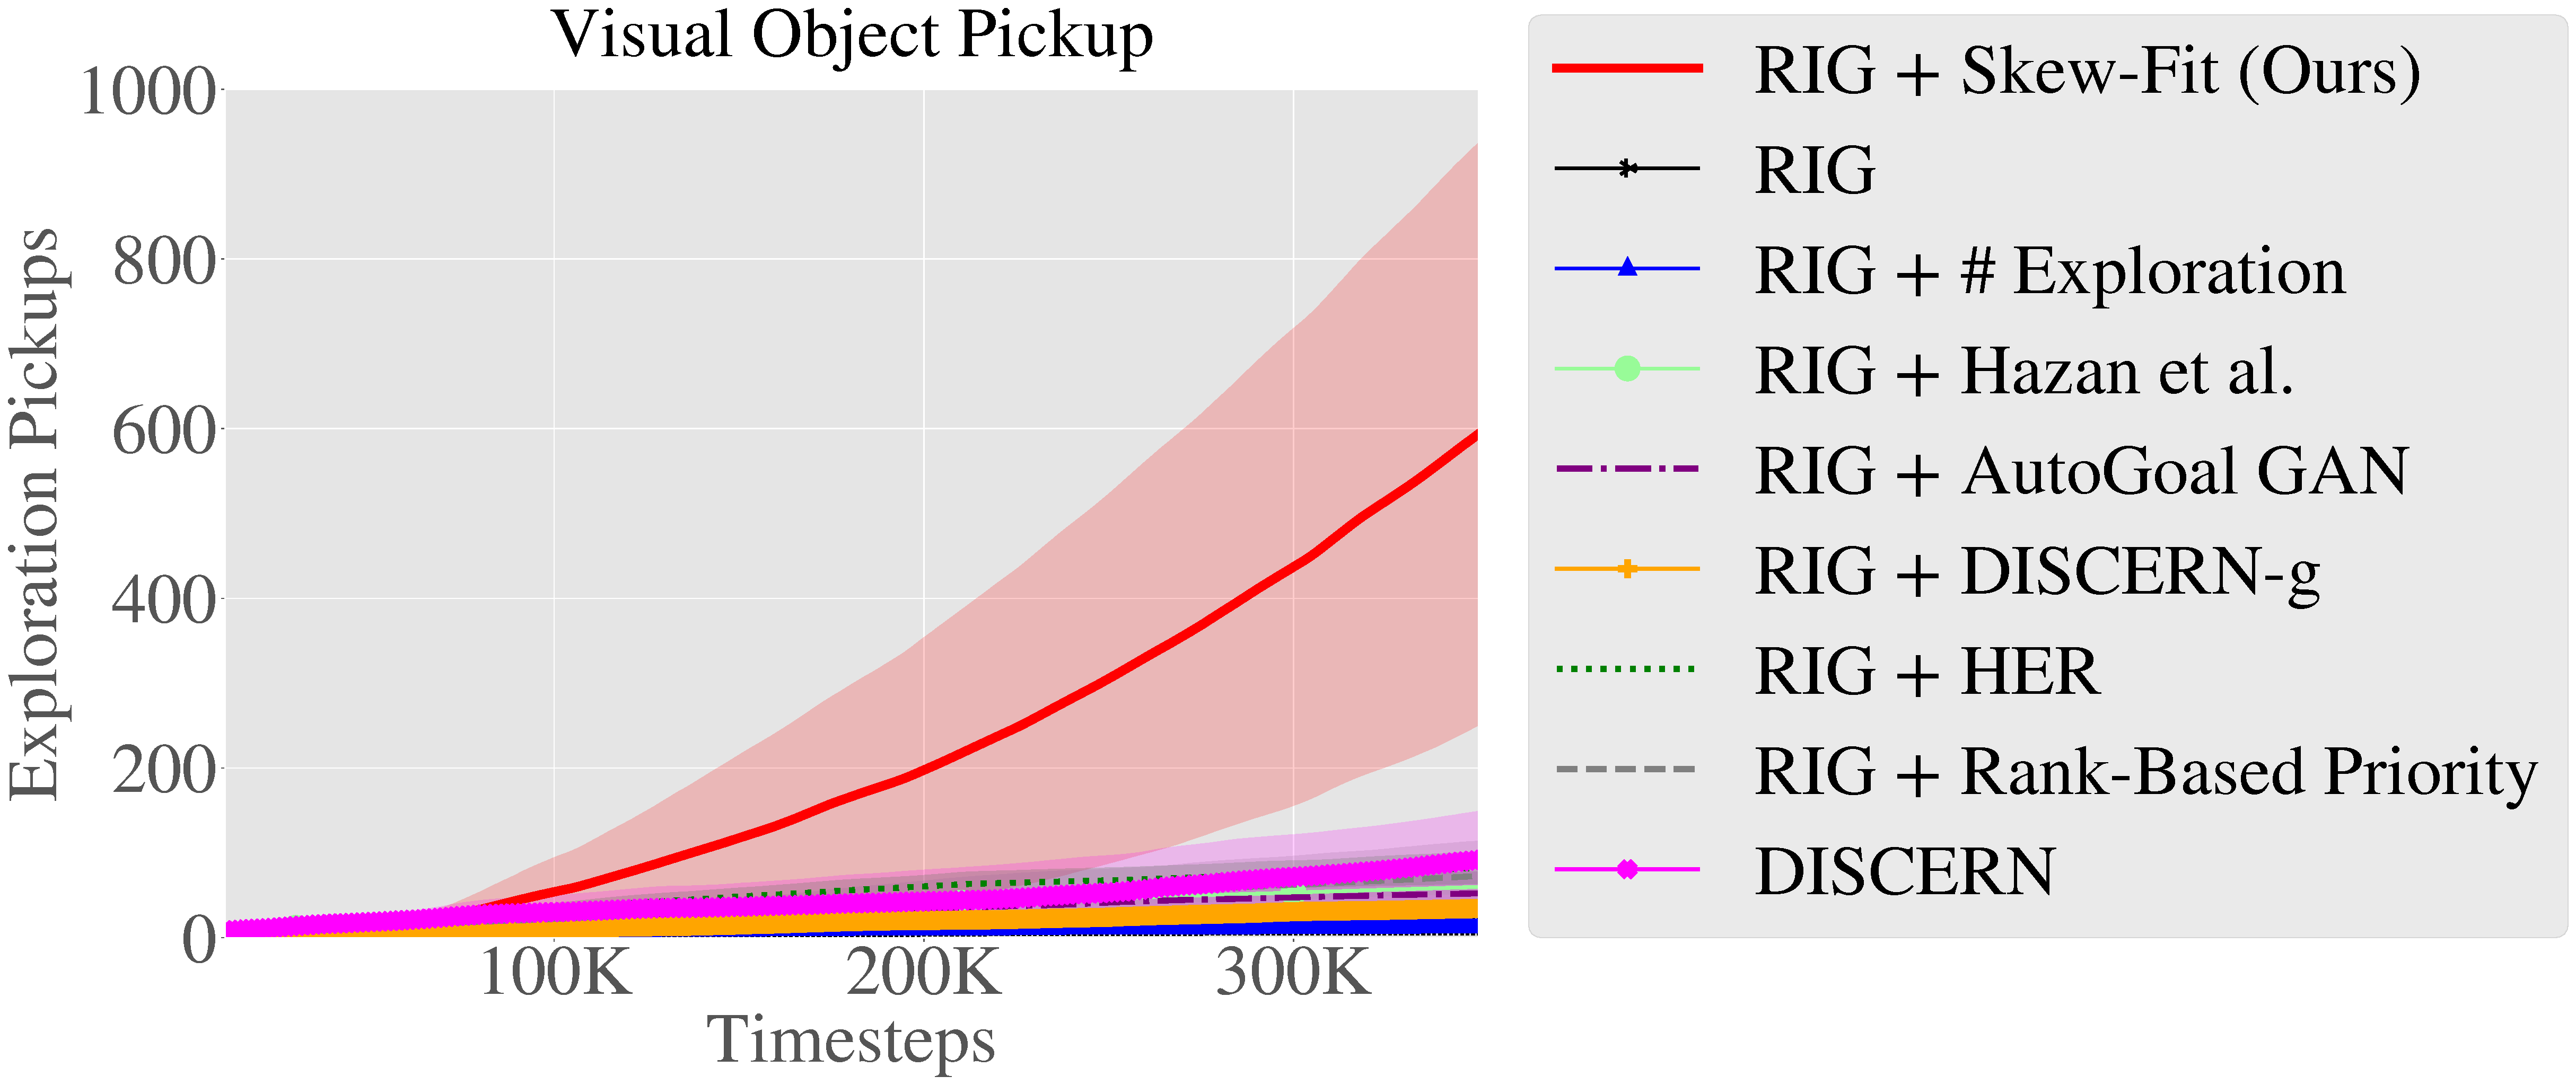
\includegraphics[width=\linewidth]{skewfit/figures/plots/exploration_pickups.pdf}
  \fcaption{
Cumulative total pickups during exploration for each method.
Prior methods fail to pay attention to the object: the rate of pickups hardly increases past the first 100 thousand timesteps.
In contrast, after seeing the object picked up a few times, \METHOD practices picking up the object more often by sampling the appropriate exploration goals.
}
  \label{fig:exploration_pickups}
\end{figure}


\paragraph{Real-World Vision-Based Robotic Manipulation}
We also demonstrate that \METHOD scales well to the real world with a door opening task, \textit{Real World Visual Door}, as shown in \Figref{fig:env-pics}.
While a number of prior works have studied RL-based learning of door opening~\cite{kalakrishnan2011learning,chebotar2017path}, we demonstrate the first method for autonomous learning of door opening without a user-provided, task-specific reward function.
As in simulation, we do not provide any goals to the agent and simply let it interact with the door, without any human guidance or reward signal.
We train two agents using RIG and RIG with \METHOD.
Every seven and a half minutes of interaction time, we evaluate on $5$ goals and plot the cumulative successes for each method.
Unlike in simulation, we cannot easily measure the difference between the policy's achieved and desired door angle.
Instead, we visually denote a binary success/failure for each goal based on whether the last state in the trajectory achieves the target angle.
As \Figref{fig:real-results} shows, standard RIG only starts to open the door after five hours of training.
In contrast, \METHOD learns to occasionally open the door after three hours of training and achieves a near-perfect success rate after five and a half hours of interaction.
\autoref{fig:real-results} also shows examples of successful trajectories from the \METHOD policy, where we see that the policy can reach a variety of user-specified goals.
These results demonstrate that \METHOD is a promising technique for solving real world tasks without any human-provided reward function.
Videos of \METHOD solving this task and the simulated tasks can be viewed on
our website.
\footnote{https://sites.google.com/view/skew-fit}

\begin{figure}[t]
  \centering
  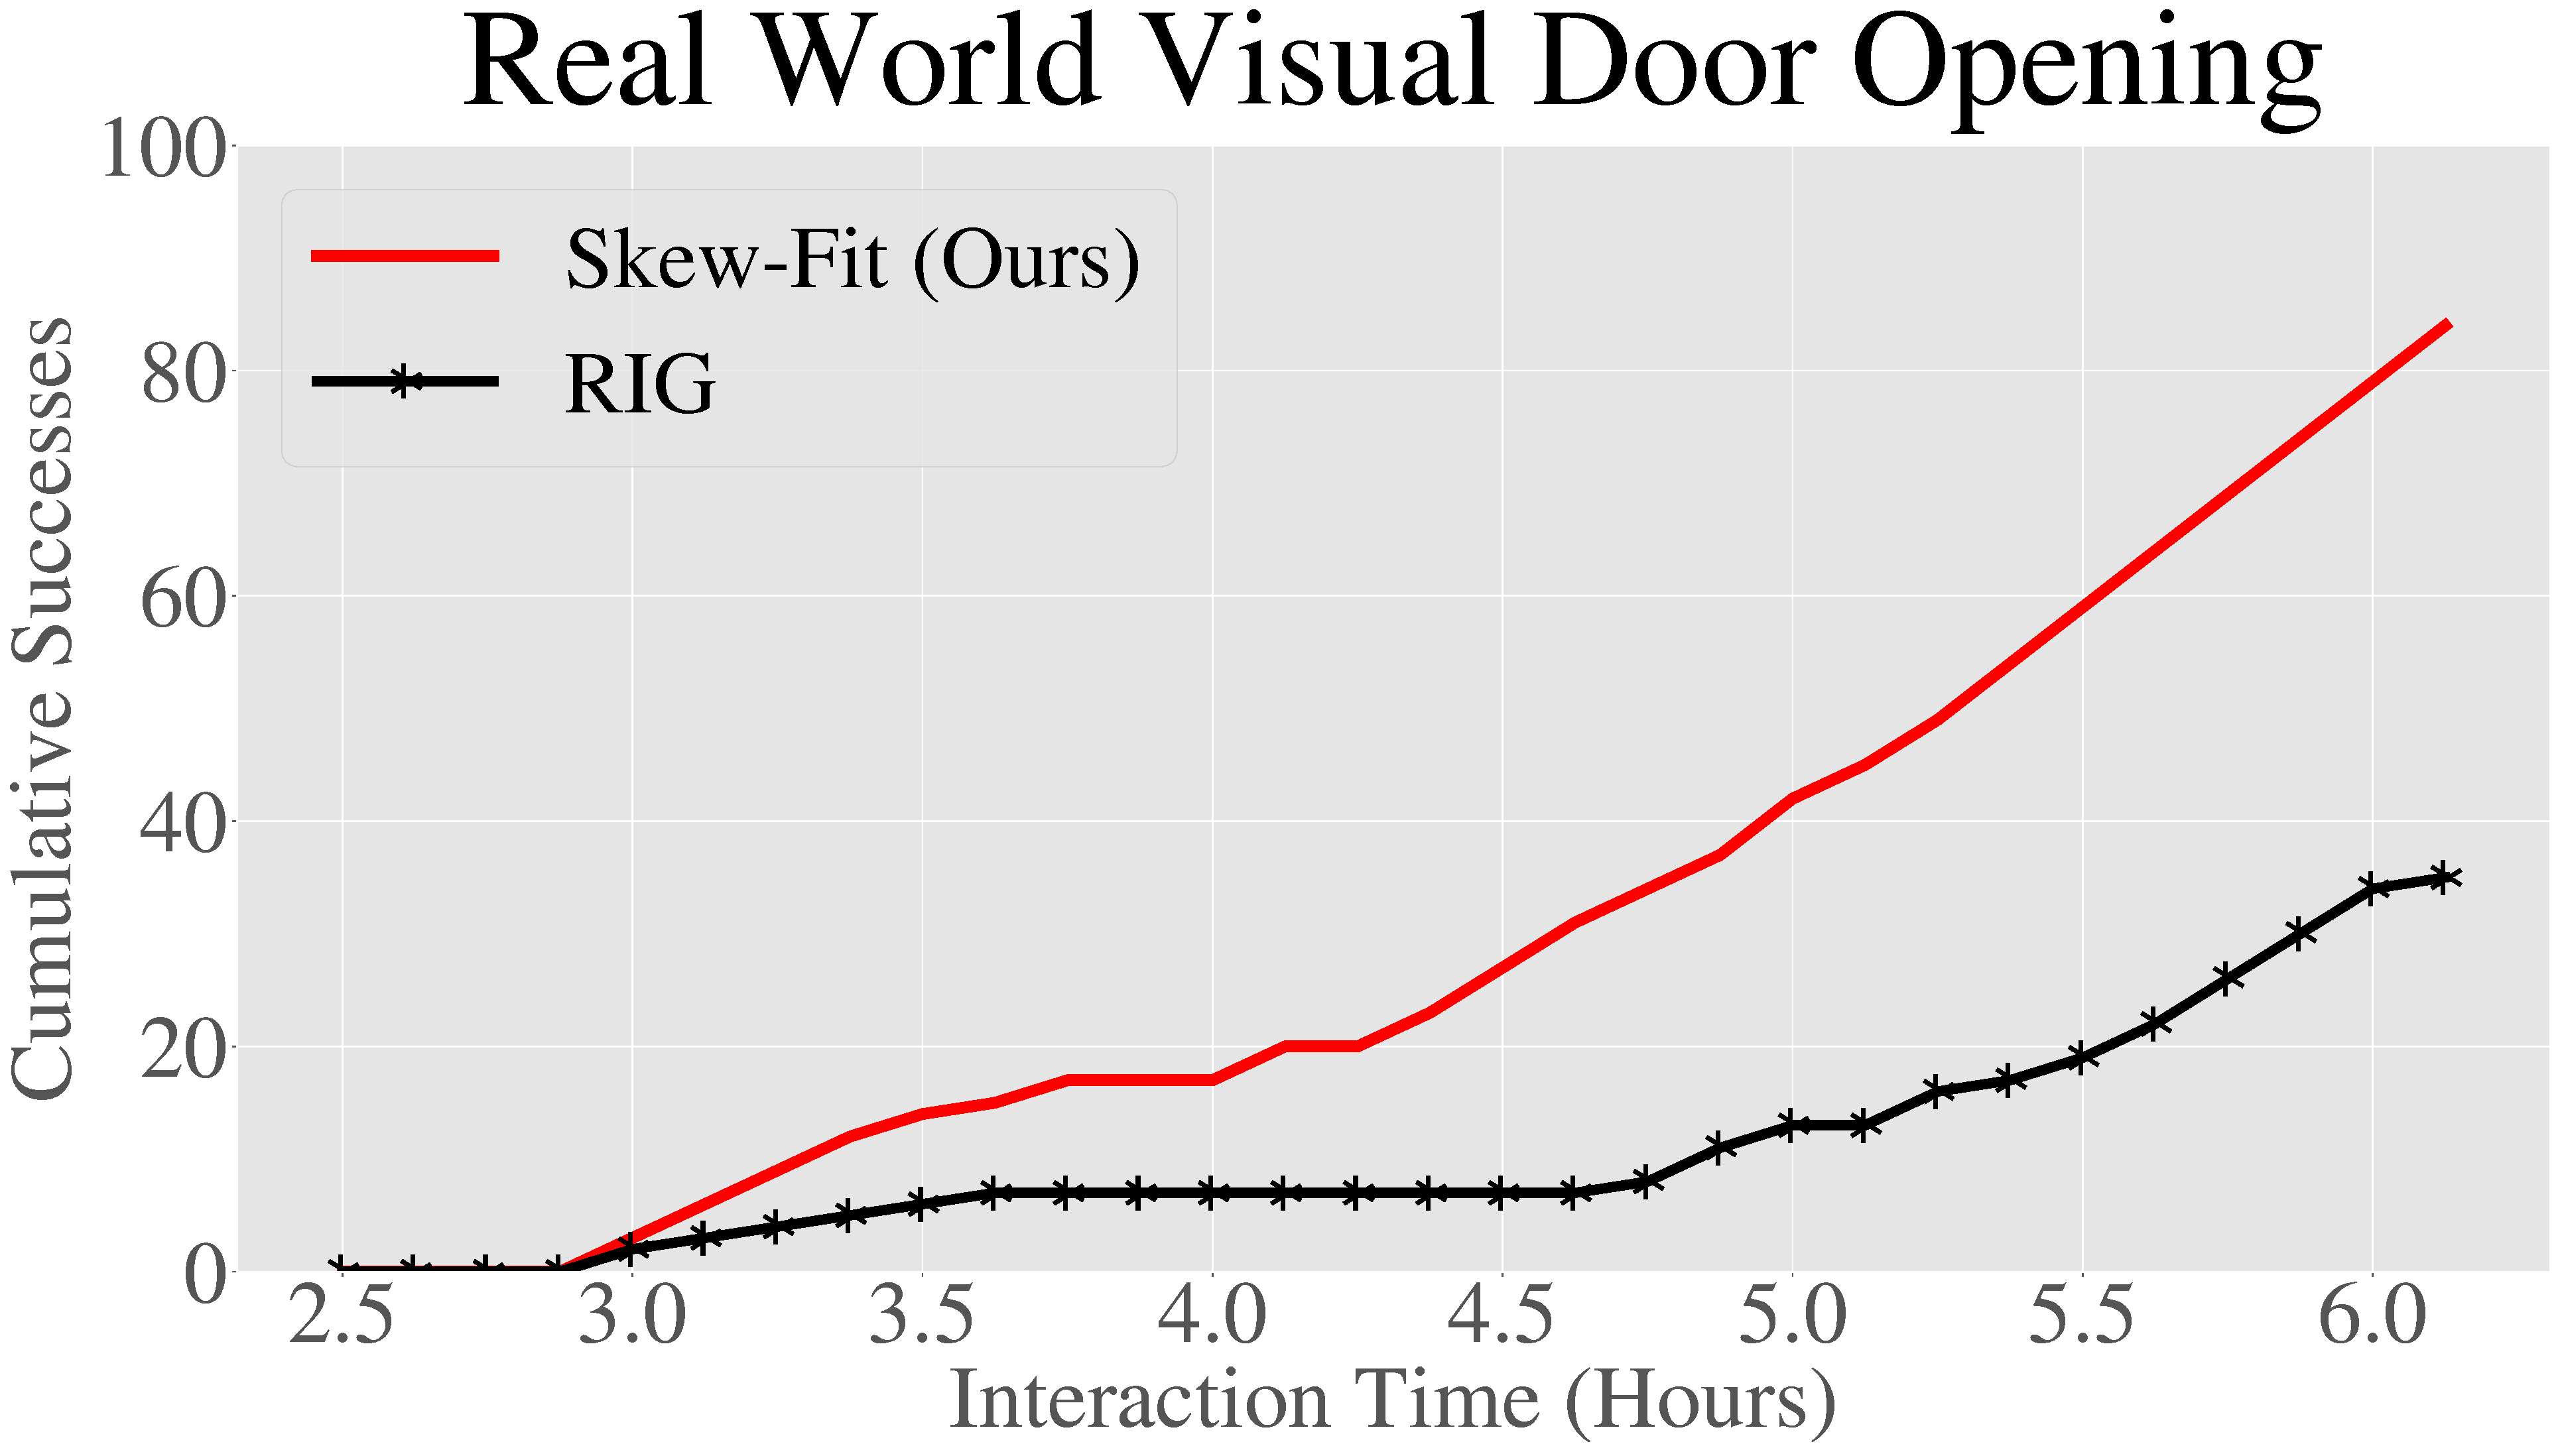
\includegraphics[width=0.75\linewidth]{skewfit/figures/plots/real_world_door.pdf}
    \begin{subfigure}[b]{0.49\textwidth}
        \center
        \hspace{-.2cm}
        $\SF_1$ \hspace{4.3cm} $\SF_{100}$ \hspace{.7cm} $\G$

        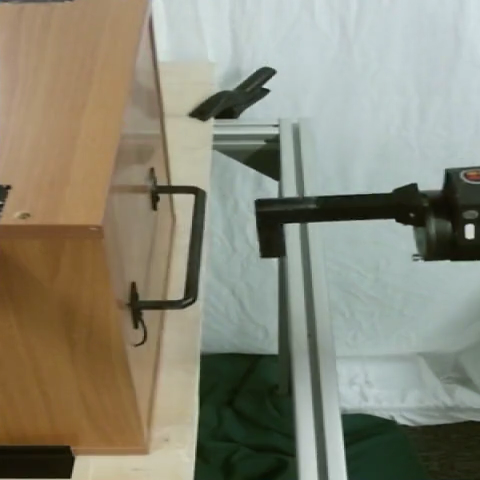
\includegraphics[width=0.14\linewidth]{skewfit/figures/imgs/real_env_rollout_new/door_easy/barely_open_5.png}
        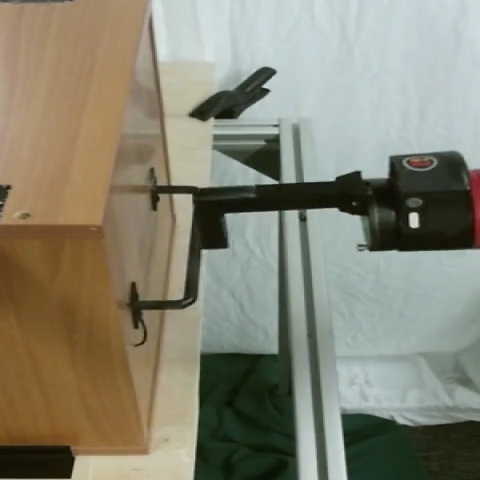
\includegraphics[width=0.14\linewidth]{skewfit/figures/imgs/real_env_rollout_new/door_easy/barely_open_10.png}
        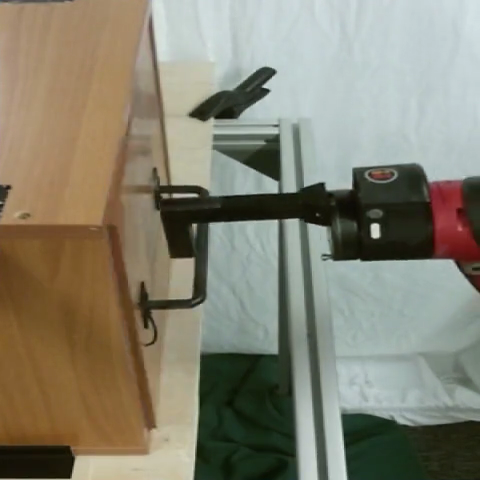
\includegraphics[width=0.14\linewidth]{skewfit/figures/imgs/real_env_rollout_new/door_easy/barely_open_15.png}
        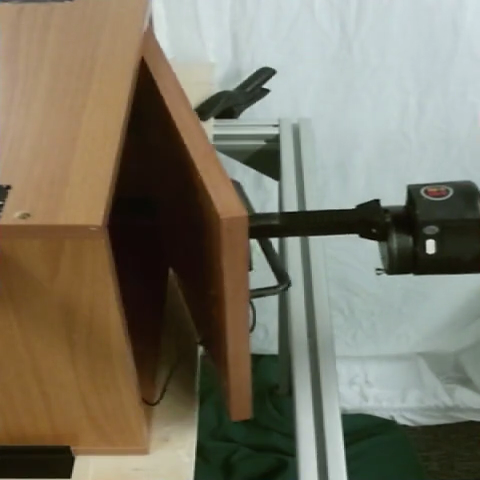
\includegraphics[width=0.14\linewidth]{skewfit/figures/imgs/real_env_rollout_new/door_easy/barely_open_20.png}
        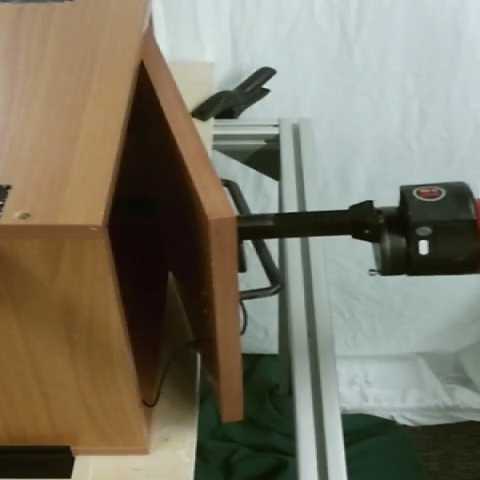
\includegraphics[width=0.14\linewidth]{skewfit/figures/imgs/real_env_rollout_new/door_easy/barely_open_25.png}
        \hspace{0.01\linewidth}
        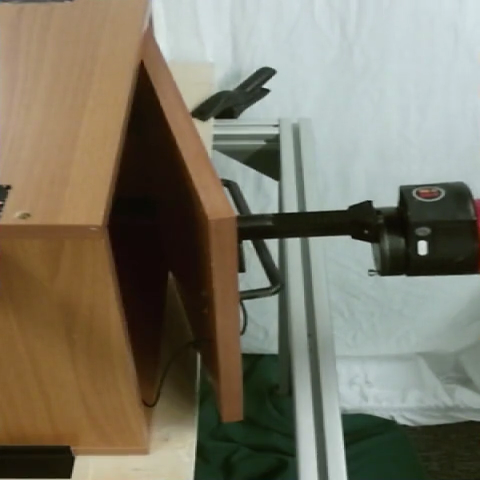
\includegraphics[width=0.14\linewidth]{skewfit/figures/imgs/real_env_rollout_new/door_easy/barely_open_45.png} %goal
    \end{subfigure}
    \begin{subfigure}[b]{0.49\textwidth}
        \center

        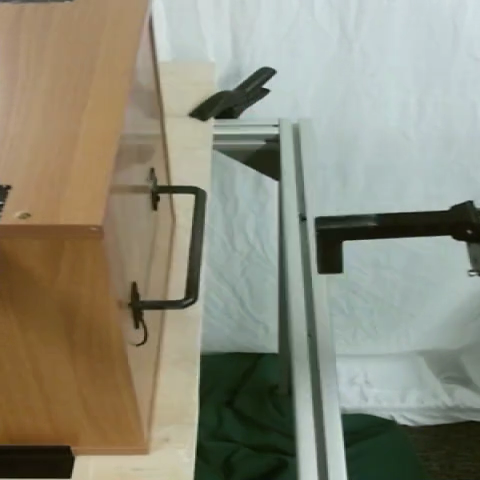
\includegraphics[width=0.14\linewidth]{skewfit/figures/imgs/real_env_rollout_novel/door_hard/wide_open_0.png}
        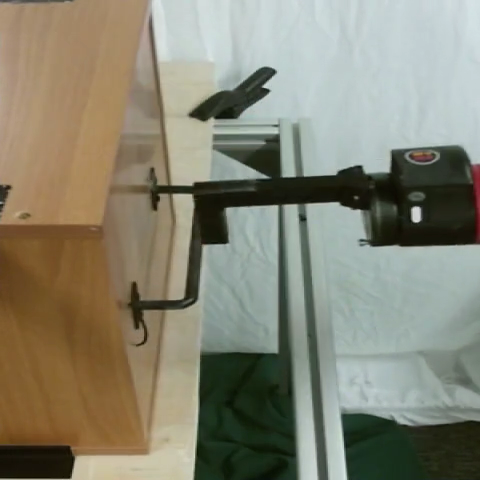
\includegraphics[width=0.14\linewidth]{skewfit/figures/imgs/real_env_rollout_novel/door_hard/wide_open_10.png}
        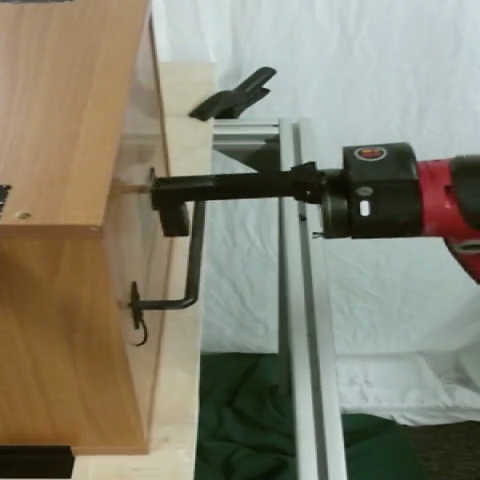
\includegraphics[width=0.14\linewidth]{skewfit/figures/imgs/real_env_rollout_novel/door_hard/wide_open_20.png}
        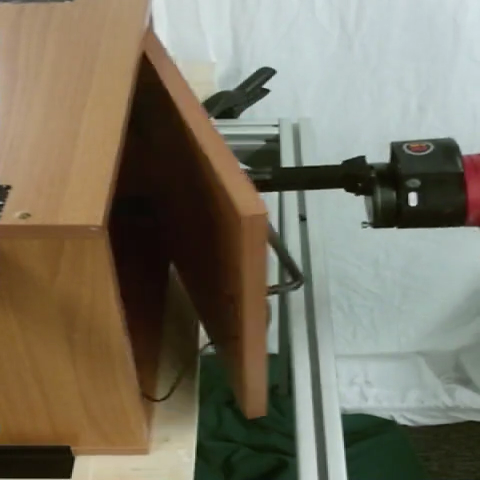
\includegraphics[width=0.14\linewidth]{skewfit/figures/imgs/real_env_rollout_novel/door_hard/wide_open_25.png}
        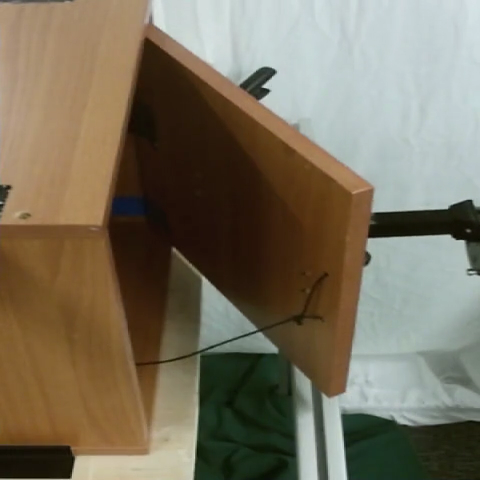
\includegraphics[width=0.14\linewidth]{skewfit/figures/imgs/real_env_rollout_novel/door_hard/wide_open_40.png}
        \hspace{0.01\linewidth}
        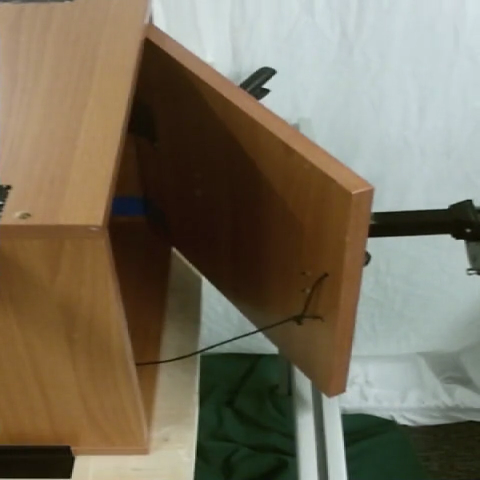
\includegraphics[width=0.14\linewidth]{skewfit/figures/imgs/real_env_rollout_novel/door_hard/wide_open_100.png}
    \end{subfigure}
  \fcaption{
  (Top) Learning curve for Real World Visual Door.
  \METHOD results in considerable sample efficiency gains over RIG on this real-world task.
  (Bottom)
  Each row shows the \METHOD policy starting from state $\SF_1$ and reaching state $\SF_{100}$ while pursuing goal $\G$.
  Despite being trained from only images without any user-provided goals during training, the \METHOD policy achieves the goal image provided at test-time, successfully opening the door.
  }
  \label{fig:real-results}
\end{figure}



\paragraph{Additional Experiments}
To study the sensitivity of \METHOD to the hyperparameter $\alpha$, we sweep $\alpha$ across the values $[-1, -0.75, -0.5, -0.25, 0]$ on the simulated image-based tasks.
The results are in \autoref{sec:add-exps} and demonstrate that \METHOD works across a large range of values for $\alpha$, and $\alpha=-1$ consistently outperform $\alpha=0$ (i.e. outperforms no \METHOD).
Additionally, \autoref{sec:implementation-details} provides a complete description our method hyperparameters, including network architecture and RL algorithm hyperparameters.

\section{Conclusion}\label{sec:conclusion}
We presented a formal objective for self-supervised goal-directed exploration, allowing researchers to quantify and compare progress when designing algorithms that enable agents to autonomously learn.
We also presented \METHOD, an algorithm for training a generative model to approximate a uniform distribution over an initially unknown set of valid states, using data obtained via goal-conditioned reinforcement learning, and our theoretical analysis gives conditions under which \METHOD converges to the uniform distribution.
When such a model is used to choose goals for exploration and to relabeling goals for training, the resulting method results in much better coverage of the state space, enabling our method to explore effectively.
Our experiments show that when we concurrently train a goal-reaching policy using self-generated goals, \METHOD produces quantifiable improvements on simulated robotic manipulation tasks, and can be used to learn a door opening skill to reach a $95\%$ success rate directly on a real-world robot, without any human-provided reward supervision.

% \section{Acknowledgement}
% This research was supported by Berkeley DeepDrive, Huawei, ARL DCIST CRA W911NF-17-2-0181, NSF IIS-1651843, and the Office of Naval Research, as well as Amazon, Google, and NVIDIA.
% We thank Aviral Kumar, Carlos Florensa, Aurick Zhou, Nilesh Tripuraneni, Vickie Ye, Dibya Ghosh, Coline Devin, Rowan McAllister, John D. Co-Reyes, various members of the Berkeley Robotic AI \& Learning (RAIL) lab, and anonymous reviewers for their insightful discussions and feedback.

% {\small
% \bibliographystyle{corlabbrvnat}
% \bibliography{main.bib}
% }

% \clearpage
% \newpage
% \pagebreak

\appendix

\section{Proofs}\label{sec:proofs}
The definitions of continuity and convergence for pseudo-metrics are similar to those for metrics, and we state them below.

A function $f: \gQ \mapsto \gQ$ is continuous with respect to a pseudo-metric $d$ if for any $p \in \gQ$ and any scalar $\epsilon > 0$, there exists a $\delta$ such that for all \mbox{$q \in \gQ$},
\begin{align*}
    d(p, q) < \delta
    \implies
    d(f(p), f(q)) < \epsilon.
\end{align*}

An infinite sequence $p_1, p_2 \dots$ converges to a value $p$ with respect to a pseudo-metric $d$, which we write as
\begin{align*}
    \limt p_t \rightarrow p,
\end{align*}
if
\begin{align*}
    \limt d(p_t, p) \rightarrow 0.
\end{align*}

Note that if $f$ is continuous, then
\begin{align*}
    \lim_{t \rightarrow \infty} \dent(p_t, q) \rightarrow 0
    \implies
    \lim_{t \rightarrow \infty} \dent(f(p_t), f(q)) \rightarrow 0.
\end{align*}

\subsection{Proof of Lemma 3.1}\label{sec:general-proof}
\begin{lemma}
Let $\Imgs$ be a compact set.
Define the set of distributions $\gQ = \{p : \support(p) \subseteq \Imgs\}$.
Let $\gF: \gQ \mapsto \gQ$ be continuous with respect to the pseudometric \mbox{$\dent(p, q) \triangleq |\gH(p) - \gH(q)|$} and $\gH(\gF(p)) \geq \gH(p)$ with equality if and only if $p$ is the uniform probability distribution on $\Imgs$, denoted as $\U$.
Define the sequence of distributions $P = (p_1, p_2, \dots)$ by starting with any $p_1 \in \gQ$ and recursively defining $p_{t+1} = \gF(p_t)$.
The sequence $P$ converges to $\U$ with respect to $\dent$. In other words, \mbox{$\lim_{t \rightarrow 0} |\gH(p_t) - \gH(\U)| \rightarrow 0$}.
\end{lemma}
\begin{proof}
The idea of the proof is to show that the distance (with respect to $\dent$) between $p_t$ and $\U$ converges to a value.
If this value is $0$, then the proof is complete since $\U$ uniquely has zero distance to itself.
Otherwise, we will show that this implies that $\gF$ is not continuous, which a contradiction.

For shorthand, define $d_t$ to be the $\dent$-distance to the uniform distribution, as in
\begin{align*}
    d_t \triangleq \dent(p_t, \U).
\end{align*}
First we prove that $d_t$ converges.
Since the entropies of the sequence $(p_1, \dots)$ monotonically increase, we have that
\begin{align*}
    d_1 \geq d_2 \geq \dots.
\end{align*}
We also know that $d_t$ is lower bounded by $0$, and so by the monotonic convergence theorem, we have that
\begin{align*}
    \lim_{t\rightarrow\infty} d_t \rightarrow d^*.
\end{align*}
for some value $d^* \geq 0$.

To prove the lemma, we want to show that $d^* = 0$.
Suppose, for contradiction, that $d^* \neq 0$.
Then consider any distribution, $q^*$, such that $\dent(q^*, \U) = d^*$.
Such a distribution always exists since we can continuously interpolate entropy values between $\gH(p_1)$ and $\gH(\U)$ with a mixture distribution.
Note that $q^* \neq \U$ since \mbox{$\dent(\U, \U) = 0$}.
Since \mbox{$\limt d_t \rightarrow d^*$}, we have that
\begin{align}\label{eq:dent-distance-goes-to-zero}
    \limt
    \dent(p_t, q^*) \rightarrow 0,
\end{align}
and so
\begin{align*}
    \limt p_t \rightarrow q^*.
\end{align*}
Because the function $\gF$ is continuous with respect to $\dent$, \autoref{eq:dent-distance-goes-to-zero} implies that
\begin{align*}
    \limt
    \dent(\gF(p_t), \gF(q^*)) \rightarrow 0.
\end{align*}
However, since $\gF(p_t) = p_{t+1}$ we can equivalently write the above equation as
\begin{align*}
    \limt
    \dent(p_{t+1}, \gF(q^*)) \rightarrow 0.
\end{align*}
which, through a change of index variables, implies that
\begin{align*}
    \limt
    p_t \rightarrow \gF(q^*)
\end{align*}
Since $q^*$ is not the uniform distribution, we have that \mbox{$\gH(\gF(q^*)) > \gH(q^*)$}, which implies that $\gF(q^*)$ and $q^*$ are unique distributions.
So, $p_t$ converges to two distinct values, $q^*$ and $\gF(q^*)$, which is a contradiction.
Thus, it must be the case that $d^* = 0$, completing the proof.
\end{proof}

%-------------------------------------------------
%-------------------------------------------------
%-------------------------------------------------
\subsection{Proof of Lemma 3.2}\label{sec:covariance-proof}
\begin{lemma}\label{lemma:covariance-general}
Given two distribution $p(x)$ and $q(x)$ where $p \ll q$ and
\begin{align}
   0 < \Cov_p[\log p(X), \log q(X)]
\end{align}
define the distribution $p_\alpha$ as
\begin{align*}
    p_\alpha(x) &= \frac{1}{Z_\alpha} p(x) q(x)^\alpha
\end{align*}
where $\alpha \in \R$ and $Z_\alpha$ is the normalizing factor.
Let $\gH_\alpha(\alpha)$ be the entropy of $p_\alpha$.
Then there exists a constant $a > 0$ such that for all $\alpha \in [-a, 0)$,
\begin{align}
    \gH_\alpha(\alpha) > \gH_\alpha(0) = \gH(p).
\end{align}

\end{lemma}
\begin{proof}
Observe that $\{p_\alpha : \alpha \in [-1, 0]\}$ is a one-dimensional exponential family
\begin{align*}
    p_\alpha(x) = e^{\alpha T(x) - A(\alpha) + k(x)}
\end{align*}
with log carrier density $k(x) = \log p(x)$, natural parameter $\alpha$, sufficient statistic $T(x) = \log q(x)$, and log-normalizer $A(\alpha) = \int_{\gX} e^{\alpha T(x) + k(x)}dx$.
As shown in \cite{nielsen2010entropies}, the entropy of a distribution from a one-dimensional exponential family with parameter $\alpha$ is given by:
\begin{align*}
    \gH_\alpha(\alpha) \triangleq
    \gH(p_\alpha)
    = A(\alpha) - \alpha A'(\alpha) - \E_{p_\alpha}[k(X)]
\end{align*}
The derivative with respect to $\alpha$ is then
\begin{align*}
    \frac{d}{d \alpha}\gH_\alpha(\alpha)
        &= - \alpha A''(\alpha) - \frac{d}{d\alpha}\E_{p_\alpha}[k(x)]\\
        &= - \alpha A''(\alpha) - \E_\alpha[k(x)(T(x) - A'(\alpha)]\\
        &= - \alpha \Var_{p_\alpha}[T(x)] - \Cov_{p_\alpha}[k(x), T(x)]
\end{align*}
where we use the fact that the $n$th derivative of $A(\alpha)$ give the $n$ central moment, i.e. $A'(\alpha) = \E_{p_\alpha}[T(x)]$ and $A''(\alpha) = \Var_{p_\alpha}[T(x)]$.
The derivative of $\alpha = 0$ is
\begin{align*}
    \frac{d}{d \alpha}\gH_\alpha(0)
        &= - \Cov_{p_0}[k(x), T(x)]\\
        &= - \Cov_p[\log p(x), \log q(x)]
\end{align*}
which is negative by assumption.
Because the derivative at $\alpha = 0$ is negative, then there exists a constant $a > 0$ such that for all $\alpha \in [-a, 0]$, $\gH_\alpha(\alpha) > \gH_\alpha(0) = \gH(p)$.
\end{proof}
The paper applies \label{lemma:covariance-general} to the case where $q = \pg$ and $p=\pstate$.
When we take $N \rightarrow \infty$, we have that $\pskewed$ corresponds to $p_\alpha$ above.

%-------------------------------------------------
%-------------------------------------------------
%-------------------------------------------------
\subsection{Simple Case Proof}\label{sec:simple-case-proof}
We prove the convergence directly for the (even more) simplified case when $\papprox = \pspgt$ using a similar technique:
\begin{lemma}\label{lemma:all-equal}
Assume the set $\Imgs$ has finite volume so that its uniform distribution $\U$ is well defined and has finite entropy.
Given any distribution $p(\st)$ whose support is $\Imgs$, recursively define $p_t$ with $p_1 = p$ and
\begin{align*}
    p_{t+1}(\st)
        &= \frac{1}{Z_\alpha^t} p_t(\st)^{\alpha}, \quad \forall \st \in \Imgs
\end{align*}
where $Z_\alpha^t$ is the normalizing constant and $\alpha \in [0, 1)$.

The sequence $(p_1, p_2, \dots)$ converges to $\U$, the uniform distribution $\Imgs$.
\end{lemma}
\begin{proof}
If $\alpha = 0$, then $p_2$ (and all subsequent distributions) will clearly be the uniform distribution.
We now study the case where $\alpha \in (0, 1)$.

At each iteration $t$, define the one-dimensional exponential family $\{\ptt : \theta \in [0, 1]\}$ where $\ptt$ is
\begin{align*}
    \ptt(\st) = e^{\theta T(\st) - A(\theta) + k(\st)}
\end{align*}
with log carrier density $k(\st) = 0$, natural parameter $\theta$, sufficient statistic $T(\st) = \log p_t(\st)$, and log-normalizer $A(\theta) = \int_{\Imgs} e^{\theta T(\st)} d\st$.
As shown in \cite{nielsen2010entropies}, the entropy of a distribution from a one-dimensional exponential family with parameter $\theta$ is given by:
\begin{align*}
    \htt(\theta) \triangleq \gH(\ptt) = A(\theta) - \theta A'(\theta)
\end{align*}
The derivative with respect to $\theta$ is then
\begin{align}\nonumber
    \frac{d}{d \theta}d\htt(\theta)
        &= - \theta A''(\theta)\\\nonumber
        &= - \theta \Var_{\st \sim \ptt}[T(\st)]\\\label{eq:easy-variance-case}
        &= - \theta \Var_{\st \sim \ptt}[\log p_t(\st)]\\\nonumber
        &\leq 0
\end{align}
where we use the fact that the $n$th derivative of $A(\theta)$ is the $n$ central moment, i.e. $A''(\theta) = \Var_{\st \sim \ptt}[T(\st)]$.
Since variance is always non-negative, this means the entropy is monotonically decreasing with $\theta$.
Note that $p_{t+1}$ is a member of this exponential family, with parameter $\theta = \alpha \in (0, 1)$.
So
\begin{align*}
    \gH(p_{t+1}) = \htt(\alpha) \geq \htt(1) = \gH(p_t)
\end{align*}
which implies
\begin{align*}
    \gH(p_1) \leq \gH(p_2) \leq \dots.
\end{align*}
This monotonically increasing sequence is upper bounded by the entropy of the uniform distribution, and so this sequence must converge.

The sequence can only converge if $\frac{d}{d \theta} \htt(\theta)$ converges to zero.
However, because $\alpha$ is bounded away from $0$, \Eqref{eq:easy-variance-case} states that this can only happen if
\begin{align}\label{eq:easy-logprob-becomes-constant}
    \Var_{\st \sim \ptt}[\log p_t(\st)] \rightarrow 0.
\end{align}
Because $p_t$ has full support, then so does $\ptt$.
Thus, \Eqref{eq:easy-logprob-becomes-constant} is only true if $\log p_t(\st)$ converges to a constant, i.e. $p_t$ converges to the uniform distribution.
\end{proof}

%-------------------------------------------------
%-------------------------------------------------
%-------------------------------------------------


\section{Additional Experiments}\label{sec:add-exps}

\subsection{Sensitivity Analysis}\label{sensitivity}
\paragraph{Sensitivity to RL Algorithm}
In our experiments, we combined \METHOD with soft actor critic (SAC)~\citep{haarnoja2018sacapp}.
We conduct a set of experiments to test whether \METHOD may be used with other RL algorithms for training the goal-conditioned policy.
To that end, we replaced SAC with twin delayed deep deterministic policy gradient (TD3)~\citep{fujimoto2018td3} and ran the same \METHOD experiments on Visual Door, Visual Pusher, and Visual Pickup.
In \autoref{fig:rl-sweep}, we see that \METHOD performs consistently well with both SAC and TD3, demonstrating that \METHOD is beneficial across multiple RL algorithms.
\begin{figure}
    \begin{subfigure}{\linewidth}
      \centering
      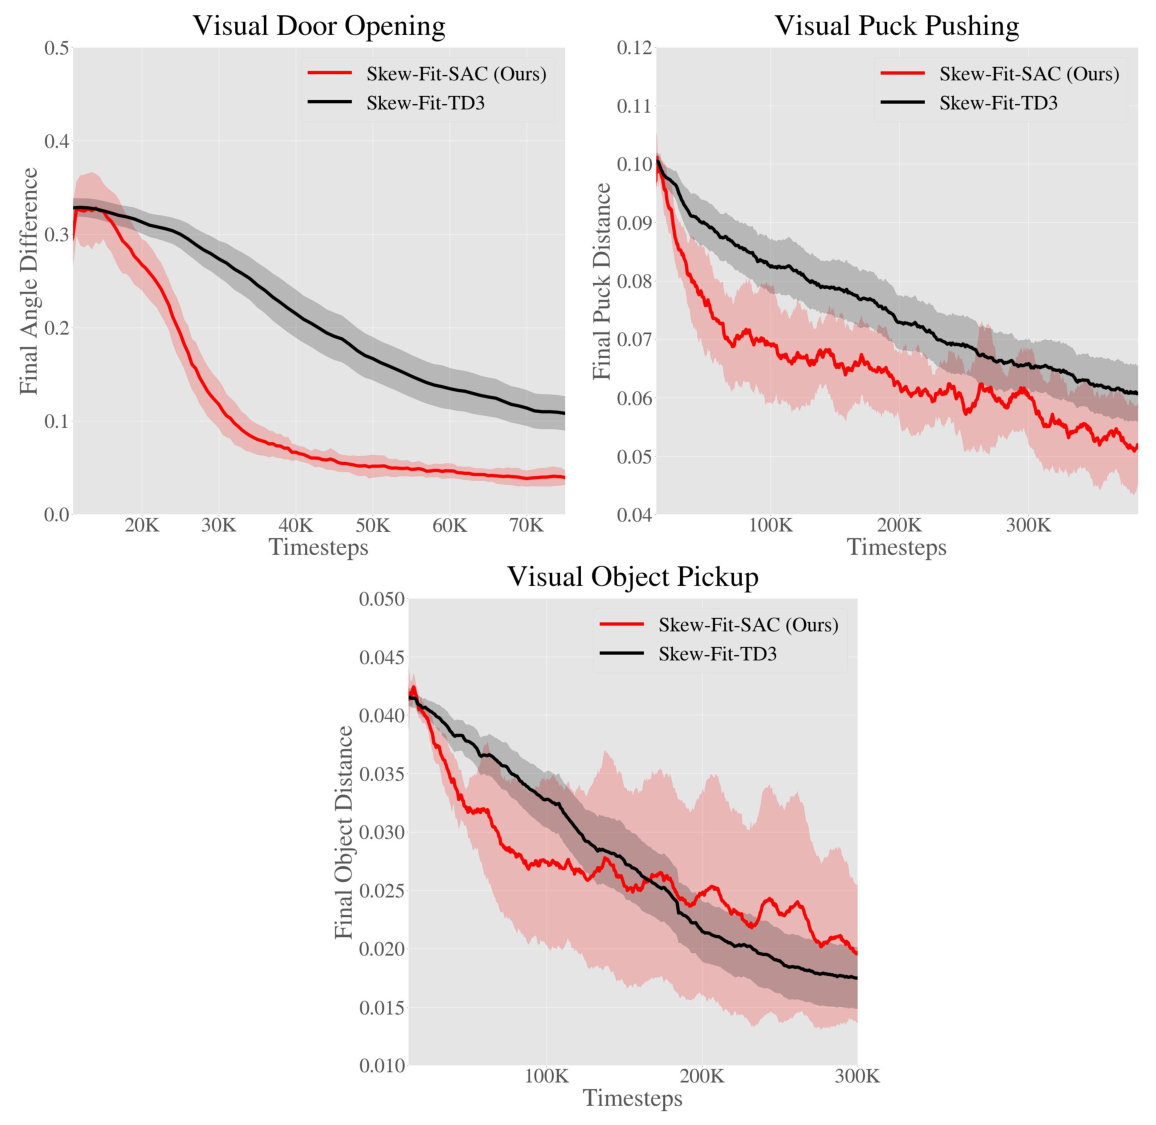
\includegraphics[width=\linewidth]{figures/plots/td3vskewfit.pdf}
      \label{fig:door-rl-sweep}
    \end{subfigure}
    \\
  \vspace{-.1in}
  \fcaption{
  We compare using SAC~\citep{haarnoja2018sacapp} and TD3~\citep{fujimoto2018td3} as the underlying RL algorithm on Visual Door, Visual Pusher and Visual Pickup.
  We see that \METHOD works consistently well with both SAC and TD3, demonstrating that \METHOD may be used with various RL algorithms.
  For the experiments presented in \autoref{sec:experiments}, we used SAC.
  }
  \vspace{-0.05 cm}
  \label{fig:rl-sweep}
\end{figure}

\paragraph{Sensitivity to $\alpha$ Hyperparameter}
We study the sensitivity of the $\alpha$ hyperparameter by testing values of \mbox{$\alpha \in [-1, -0.75, -0.5, -0.25, 0]$} on the Visual Door and Visual Pusher task.
The results are included in \Figref{fig:alpha-sweep} and shows that our method is  robust to different parameters of $\alpha$, particularly for the more challenging Visual Pusher task.
Also, the method consistently outperform $\alpha=0$, which is equivalent to sampling uniformly from the replay buffer.
\begin{figure}[!ht]
  \centering
  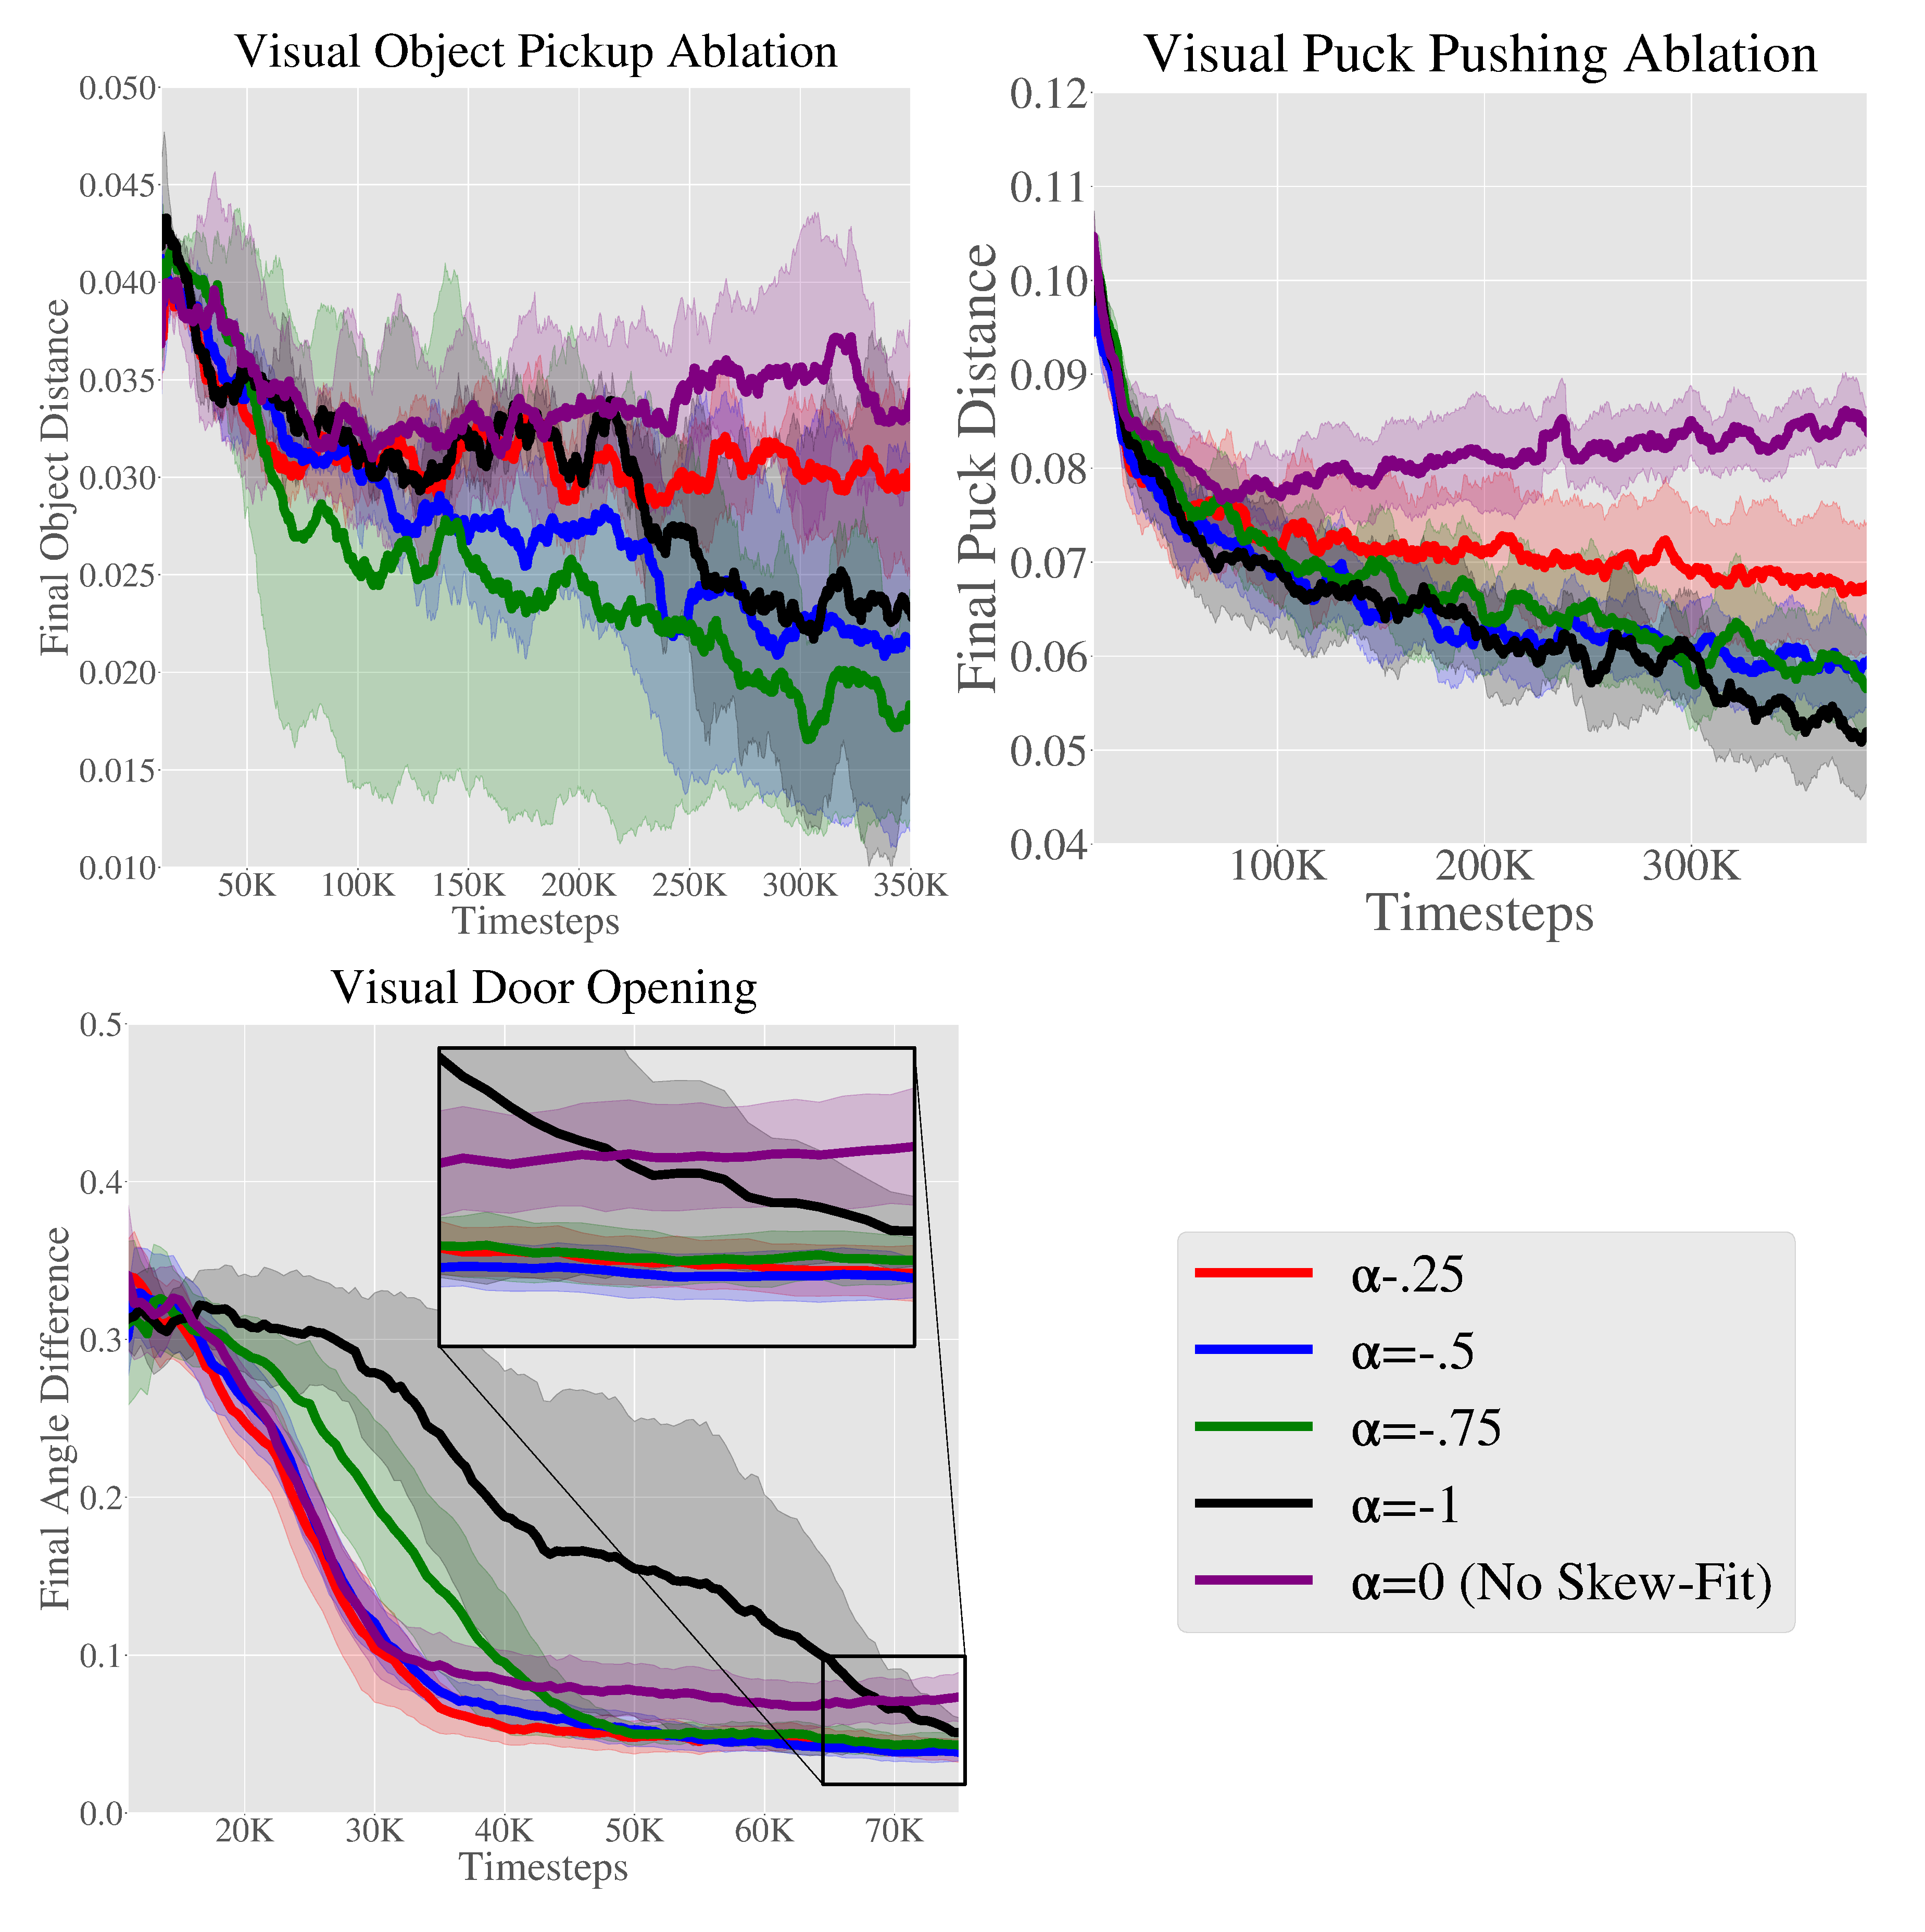
\includegraphics[width=1\linewidth]{figures/plots/power_ablation_square_with_inset.pdf}
  \vspace{-.05in}
  \label{fig:door-alpha-sweep}
  \vspace{-.1in}
  \fcaption{
  We sweep different values of $\alpha$ on Visual Door, Visual Pusher and Visual Pickup.
  \METHOD helps the final performance on the Visual Door task, and outperforms No Skew-Fit ($\alpha=0$) as seen in the zoomed in version of the plot.
  In the more challenging Visual Pusher task, we see that \METHOD consistently helps and halves the final distance.
  Similarly, we observe that \METHOD consistently outperforms No Skew-fit on Visual Pickup.
  Note that alpha=-1 is not always the optimal setting for each environment, but outperforms $\alpha=0$ in each case in terms of final performance.
  }
  \vspace{-0.05 cm}
  \label{fig:alpha-sweep}
\end{figure}

 \subsection{Variance Ablation} \label{sec:analysis-variance}
 \begin{figure}[H]
     \vspace{0.1in}
         \centering
         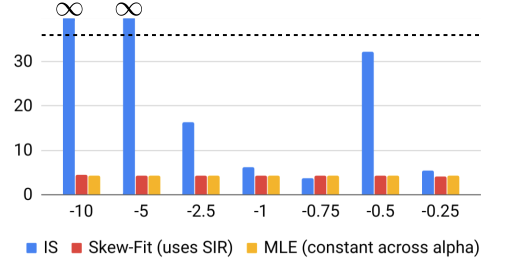
\includegraphics[width=0.8\linewidth]{figures/plots/variance.png}
         \fcaption{Gradient variance averaged across parameters in last epoch of training VAEs. Values of $\alpha$ less than $-1$ are numerically unstable for importance sampling (IS), but not for Skew-Fit.}
         \label{fig:grad-var}
     \label{fig:ul-variance-results}
 \end{figure}
We measure the gradient variance of training a VAE on an unbalanced Visual Door image dataset with \METHOD vs \METHOD with importance sampling (IS) vs no \METHOD (labeled MLE). We construct the imbalanced dataset by rolling out a random policy in the environment and collecting the visual observations. Most of the images contained the door in a closed position; in a few, the door was opened.
 In \autoref{fig:ul-variance-results}, we see that the gradient variance for Skew-Fit with IS is catastrophically large for large values of $\alpha$.
 In contrast, for Skew-Fit with SIR, which is what we use in practice, the variance is relatively similar to that of MLE. Additionally we trained three VAE's, one with MLE on a uniform dataset of valid door opening images, one with Skew-Fit on the unbalanced dataset from above, and one with MLE on the same unbalanced dataset. As expected, the VAE that has access to the uniform dataset gets the lowest negative log likelihood score.
 This is the oracle method, since in practice we would only have access to imbalanced data.
 As shown in \autoref{table:ll-ablation}, \METHOD considerably outperforms MLE, getting a much closer to oracle log likelihood score.
 \begin{table}
         \centering
         \begin{tabular}{|l|l|}
         \hline
             {\footnotesize \textbf{Method}}                 & {\footnotesize \textbf{NLL}}   \\\hline
             {\footnotesize MLE on uniform (oracle)} & {\footnotesize 20175.4}               \\\hline
             {\footnotesize Skew-Fit on unbalanced}           & {\footnotesize 20175.9}              \\\hline
             {\footnotesize MLE on unbalanced}                    & {\footnotesize 20178.03} \\\hline
         \end{tabular}
         \fcaption{Despite training on a unbalanced Visual Door dataset (see Figure 7 of paper), the negative log-likelihood (NLL) of Skew-Fit evaluated on a uniform dataset matches that of a VAE trained on a uniform dataset.}
         \label{table:ll-ablation}
 \end{table}


\subsection{Goal and Performance Visualization}\label{sec:vae-dump}
We visualize the goals sampled from \METHOD as well as those sampled when using the prior method, RIG~\citep{nair2018rig}.
As shown in \autoref{fig:vae_dump} and \autoref{fig:vae_dump_real}, the generative model $\pg$ results in much more diverse samples when trained with \METHOD.
We we see in \autoref{fig:example_rollouts}, this results in a policy that more consistently reaches the goal image.
\begin{figure*}
    \centering
    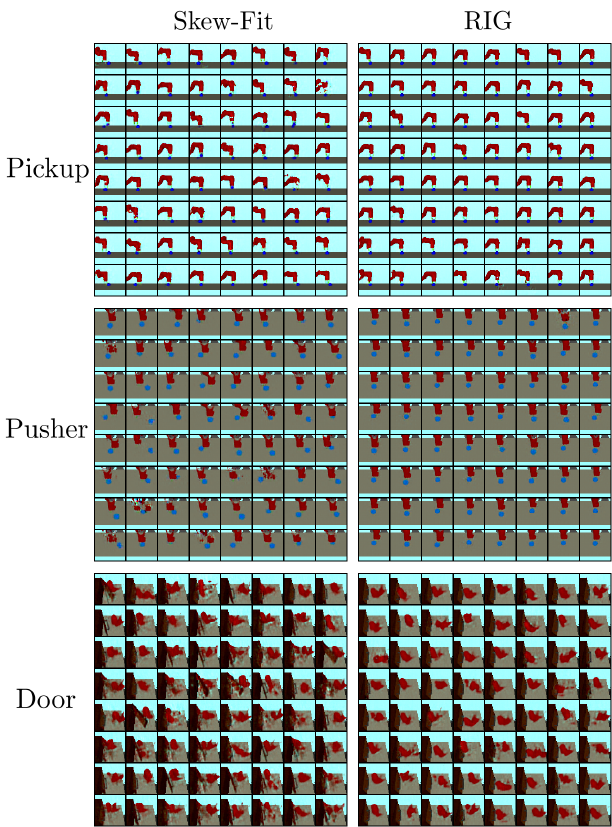
\includegraphics[width=0.9\textwidth]{figures/vae_samples_v3-01.png}
    \fcaption{
Proposed goals from the VAE for RIG and with \METHOD on the \textit{Visual Pickup}, \textit{Visual Pusher}, and \textit{Visual Door} environments. Standard RIG produces goals where the door is closed and the object and puck is in the same position, while RIG + \METHOD proposes goals with varied puck positions, occasional object goals in the air, and both open and closed door angles.
    }
    \label{fig:vae_dump}
\end{figure*}

\begin{figure*}
    \centering
    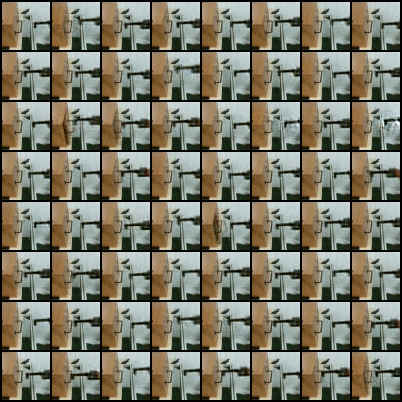
\includegraphics[width=0.25\textheight]{figures/vae_dumps/rig-real-world-v2-exp-samples.png}
    \hspace{.3 in}
    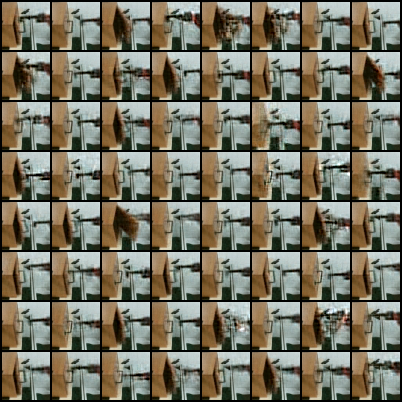
\includegraphics[width=0.25\textheight]{figures/vae_dumps/skew-fit-real-world-v2-exp-samples.png}
    \fcaption{
Proposed goals from the VAE for RIG (left) and with RIG + \METHOD (right) on the \textit{Real World Visual Door} environment. Standard RIG produces goals where the door is closed  while RIG + \METHOD proposes goals with both open and closed door angles.
    }
    \label{fig:vae_dump_real}
\end{figure*}
\begin{figure*}
    \centering
    \includegraphics[width=0.9\textwidth]{figures/example-rollouts.jpg}
    \fcaption{
Example reached goals by \METHOD and RIG. The first column of each environment section specifies the target goal while the second and third columns show reached goals by \METHOD and RIG. Both methods learn how to reach goals close to the initial position, but only \METHOD learns to reach the more difficult goals.
    }
    \label{fig:example_rollouts}
\end{figure*}

\section{Implementation Details}\label{sec:implementation-details}

\subsection{Likelihood Estimation using $\beta$-VAE}\label{sec:likelihood-estimation-vae}
We estimate the density under the VAE by using a sample-wise approximation to the marginal over $x$ estimated using importance sampling:
\begin{align*}
    \pgt(x) &= \mathbb E_{z \sim q_{\theta_t}(z|x)} \left[\frac{p(z)}{q_{\theta_t}(z|x)} p_{\psi_t}(x \mid z) \right]  \\
    &\approx \frac{1}{N} \sum_{i=1}^{N} \left[\frac{p(z)}{q_{\theta_t}(z|x)} p_{\psi_t}(x \mid z) \right].
\end{align*}
where $q_{\theta}$ is the encoder, $p_\psi$ is the decoder, and $p(z)$ is the prior, which in this case is unit Gaussian.
We found that sampling $N=10$ latents for estimating the density worked well in practice.

\subsection{Oracle 2D Navigation Experiments}\label{sec:2d-details}
We initialize the VAE to the bottom left corner of the environment for \textit{Four Rooms}.
Both the encoder and decoder have 2 hidden layers with [400, 300] units,  ReLU hidden activations, and no output activations.
The VAE has a latent dimension of $8$ and a Gaussian decoder trained with a fixed variance, batch size of $256$, and $1000$ batches at each iteration. The VAE is trained on the exploration data buffer every 1000 rollouts.

\subsection{Implementation of SAC and Prior Work}\label{sec:prior-work-implementation}
For all experiments, we trained the goal-conditioned policy using soft actor critic (SAC)~\citep{haarnoja2018sacapp}.
To make the method goal-conditioned, we concatenate the target XY-goal to the state vector.
During training, we retroactively relabel the goals~\citep{kaelbling1993goals,andrychowicz2017her} by sampling from the goal distribution with probabilty $0.5$.
Note that the original RIG~\cite{nair2018rig} paper used TD3~\cite{fujimoto2018td3}, which we also replaced with SAC in our implementation of RIG.
We found that maximum entropy policies in general improved the performance of RIG, and that we did not need to add noise on top of the stochastic policy's noise.
In the prior RIG method, the VAE was pre-trained on a uniform sampling of images from the state space of each environment.
In order to ensure a fair comparison to Skew-Fit, we forego pre-training and instead train the VAE alongside RL, using the variant described in the RIG paper.
For our RL network architectures and training scheme, we use fully connected networks for the policy, Q-function and value networks with two hidden layers of size $400$ and $300$ each.
We also delay training any of these networks for $10000$ time steps in order to collect sufficient data for the replay buffer as well as to ensure the latent space of the VAE is relatively stable (since we continuously train the VAE concurrently with RL training).
As in RIG, we train a goal-conditioned value functions~\cite{schaul2015uva} using hindsight experience replay~\cite{andrychowicz2017her}, relabelling $50\%$ of exploration goals as goals sampled from the VAE prior $\mathcal{N} (0, 1)$ and $30\%$ from future goals in the trajectory.

For our implementation of \citep{hazan2019provably}, we trained the policies with the reward
\begin{align*}
    r(s) = r_\text{Skew-Fit}(s) + \lambda \cdot r_\text{Hazan et al.}(s)
\end{align*}

For $r_\text{Hazan et al.}$, we use the reward described in Section 5.2 of \citet{hazan2019provably}, which requires an estimated likelihood of the state.
To compute these likelihood, we use the same method as in Skew-Fit (see \autoref{sec:likelihood-estimation-vae}).
With 3 seeds each, we tuned $\lambda$ across values $[100, 10, 1, 0.1, 0.01, 0.001]$ for the door task, but all values performed poorly.
For the pushing and picking tasks, we tested values across $[1, 0.1, 0.01, 0.001, 0.0001]$ and found that 0.1 and 0.01 performed best for each task, respectively.

\subsection{RIG with \METHOD Summary}\label{sec:rig-and-full-method}
\autoref{alg:rig-and-full-method-details} provides detailed pseudo-code for how we combined our method with RIG.
Steps that were removed from the base RIG algorithm are highlighted in blue and steps that were added are highlighted in red.
The main differences between the two are (1) not needing to pre-train the $\beta$-VAE, (2) sampling exploration goals from the buffer using $\pskewed$ instead of the VAE prior, (3) relabeling with replay buffer goals sampled using $\pskewed$ instead of from the VAE prior, and (4) training the VAE on replay buffer data data sampled using $\pskewed$ instead of uniformly.

\subsection{Vision-Based Continuous Control Experiments}\label{sec:vision-based-appendix}
In our experiments, we use an image size of 48x48.
For our VAE architecture, we use a modified version of the architecture used in the original RIG paper ~\cite{nair2018rig}.
Our VAE has three convolutional layers with kernel sizes: 5x5, 3x3, and 3x3, number of output filters: 16, 32, and 64 and strides: 3, 2, and 2.
We then have a fully connected layer with the latent dimension number of units, and then reverse the architecture with de-convolution layers.
We vary the latent dimension of the VAE, the $\beta$ term of the VAE and the $\alpha$ term for \METHOD based on the environment.
Additionally, we vary the training schedule of the VAE based on the environment. See the table at the end of the appendix for more details.
Our VAE has a Gaussian decoder with identity variance, meaning that we train the decoder with a mean-squared error loss.

When training the VAE alongside RL, we found the following three schedules to be effective for different environments:

\begin{enumerate}
    \item For first $5K$ steps: Train VAE using standard MLE training every $500$ time steps for $1000$ batches. After that, train VAE using \METHOD every $500$ time steps for $200$ batches.
    \item For first $5K$ steps: Train VAE using standard MLE training every $500$ time steps for $1000$ batches. For the next $45K$ steps, train VAE using \METHOD every $500$ steps for $200$ batches. After that, train VAE using \METHOD every $1000$ time steps for $200$ batches.
    \item For first $40K$ steps: Train VAE using standard MLE training every $4000$ time steps for $1000$ batches. Afterwards, train VAE using \METHOD every $4000$ time steps for $200$ batches.
\end{enumerate}

We found that initially training the VAE without \METHOD improved the stability of the algorithm.
This is due to the fact that density estimates under the VAE are constantly changing and inaccurate during the early phases of training. Therefore, it made little sense to use those estimates to prioritize goals early on in training.
Instead, we simply train using MLE training for the first $5K$ timesteps, and after that we perform \METHOD according to the VAE schedules above. Table \ref{table:general-hyperparams} lists the hyper-parameters that were shared across the continuous control experiments. Table \ref{table:env-hyperparams} lists hyper-parameters specific to each environment. Additionally, \autoref{sec:rig-and-full-method} discusses the combined RIG + Skew-Fit algorithm.

\begin{table*}
    \centering
    \begin{tabular}{c|c|c}
    \hline
    \textbf{Hyper-parameter} & \textbf{Value} & \textbf{Comments}\\
    \hline
    \# training batches per time step & $2$ & Marginal improvements after $2$\\
    Exploration Noise & None (SAC policy is stochastic) & Did not tune\\
    RL Batch Size & $1024$ & smaller batch sizes work as well\\
    VAE Batch Size &  $64$ & Did not tune \\
    Discount Factor & $0.99$ & Did not tune\\
    Reward Scaling & $1$ & Did not tune\\
    Policy Hidden Sizes & $[400, 300]$ & Did not tune\\
    Policy Hidden Activation & ReLU & Did not tune\\
    Q-Function Hidden Sizes & $[400, 300]$ & Did not tune\\
    Q-Function Hidden Activation & ReLU & Did not tune\\
    Replay Buffer Size & $100000$ & Did not tune\\
    Number of Latents for Estimating Density ($N$) & $10$ & Marginal improvements beyond $10$\\
    \hline
    \end{tabular}
\fcaption{General hyper-parameters used for all \textit{visual} experiments.}
\label{table:general-hyperparams}
\end{table*}



\begin{table*}
    \centering
    \begin{tabular}{c|c|c|c|c}
    \hline
    \textbf{Hyper-parameter} & \textbf{Visual Pusher} & \textbf{Visual Door} & \textbf{Visual Pickup} & \textbf{Real World Visual Door}\\
    \hline
    Path Length & $50$& $100$ & $50$ & $100$ \\
    $\beta$ for $\beta$-VAE & $20$ & $20$ & $30$ & $60$ \\
    Latent Dimension Size & $4$ & $16$ & $16$ & $16$ \\
    $\alpha$ for Skew-Fit & $-1$ & $-1/2$ & $-1$ & $-1/2$ \\
    VAE Training Schedule & $2$ & $1$ & $2$ & $1$ \\
    Sample Goals From & $\pg$ & $\pskewed$ & $\pskewed$ & $\pskewed$ \\
    \hline
    \end{tabular}
\fcaption{Environment specific hyper-parameters for the \textit{visual} experiments}
\label{table:env-hyperparams}
\end{table*}

\begin{table*}
    \centering
    \begin{tabular}{c|c}
    \hline
    \textbf{Hyper-parameter} & \textbf{Value} \\
    \hline
    \# training batches per time step & $.25$\\
    Exploration Noise & None (SAC policy is stochastic) \\
    RL Batch Size & $512$\\
    VAE Batch Size &  $64$\\
    Discount Factor & $\frac{299}{300}$\\
    Reward Scaling & $10$\\
    Path length & $300$\\
    Policy Hidden Sizes & $[400, 300]$\\
    Policy Hidden Activation & ReLU\\
    Q-Function Hidden Sizes & $[400, 300]$\\
    Q-Function Hidden Activation & ReLU\\
    Replay Buffer Size & $1000000$\\
    Number of Latents for Estimating Density ($N$) & $10$\\
    $\beta$ for $\beta$-VAE & $10$ \\
    Latent Dimension Size & $2$ \\
    $\alpha$ for Skew-Fit & $-2.5$ \\
    VAE Training Schedule & $3$ \\
    Sample Goals From & $\pskewed$ \\
    \hline
    \end{tabular}
\fcaption{Hyper-parameters used for the \textit{ant} experiment.}
\label{table:ant-hyperparams}
\end{table*}


\begin{algorithm}
   	\footnotesize
   	\fcaption{RIG and RIG + Skew-Fit. Blue text denotes RIG specific steps and red text denotes RIG + Skew-Fit specific steps}
   	\label{alg:rig-and-full-method-details}
   	\begin{algorithmic}[1]
    \REQUIRE $\beta$-VAE mean encoder $q_\phi$, $\beta$-VAE decoder $p_\psi$, policy $\pi_\theta$, goal-conditioned value function $Q_w$, skew parameter $\alpha$, VAE Training Schedule.
    \STATE \textcolor{blue}{Collect $\mathcal D = \{s^{(i)}\}$ using random initial policy.}
    \STATE \textcolor{blue}{Train $\beta$-VAE on data uniformly sampled from $\mathcal D$}.
    \STATE \textcolor{blue}{Fit prior $p(z)$ to latent encodings $\{\mu_\phi(s^{(i)})\}$.}
    \FOR{$n=0,...,N-1$ episodes}
        \STATE \textcolor{blue}{Sample latent goal from prior $z_g \sim p(z)$}.
        \STATE \textcolor{red}{Sample state $s_g \sim \pskewedn$ and encode $z_g = q_\phi(s_g)$ if $\mathcal R$ is nonempty. Otherwise sample $z_g \sim p(z)$}
        \STATE Sample initial state $s_0$ from the environment.
        \FOR{$t=0,...,H -1$ steps}
            \STATE Get action $a_t \sim \pi_\theta(q_\phi(s_t), z_g)$.
            \STATE Get next state $s_{t+1} \sim p(\cdot \mid s_t, a_t)$.
            \STATE Store $(s_t, a_t, s_{t+1}, z_g)$ into replay buffer $\mathcal R$.
            \STATE Sample transition $(s, a, s', z_g) \sim \mathcal R$.
            \STATE Encode $z = q_\phi(s), z' = q_\phi(s')$.
            \STATE \textcolor{blue}{(Probability $0.5$) replace $z_g$ with $z_g' \sim p(z)$.}
            \STATE \textcolor{red}{(Probability $0.5$) replace $z_g$ with $q_\phi(s'')$ where $s'' \sim \pskewedn$.}
            \STATE Compute new reward $r = -||z' - z_g||$.
            \STATE Minimize Bellman Error using $(z, a, z', z_g, r)$.
        \ENDFOR
        \FOR{$t=0,...,H -1$ steps}
            \FOR{$i=0,...,k-1$ steps}
                \STATE Sample future state $s_{h_i}$, $t < h_i \leq H-1$.
                \STATE Store $(s_t, a_t, s_{t+1}, q_\phi(s_{h_i}))$ into $\mathcal R$.
            \ENDFOR
        \ENDFOR
        \STATE \textcolor{red}{Construct skewed replay buffer distribution $\pskewednn$ using data from $\mathcal R$ with \Eqref{eq:pskew-defn}.}
        \IF {total steps $< 5000$}
            \STATE Fine-tune $\beta$-VAE on data uniformly sampled from $\mathcal R$ according to VAE Training Schedule.
        \ELSE
            \STATE \textcolor{blue}{Fine-tune $\beta$-VAE on data uniformly sampled from $\mathcal R$ according to VAE Training Schedule.}
            \STATE \textcolor{red}{Fine-tune $\beta$-VAE on data sampled from $\pskewednn$ according to VAE Training Schedule.}
        \ENDIF
    \ENDFOR
   	\end{algorithmic}
\end{algorithm}

\section{Environment Details}\label{sec:environment-details}
\textit{Four Rooms}: A 20 x 20 2D pointmass environment in the shape of four rooms~\citep{sutton1999between}. The observation is the 2D position of the agent, and the agent must specify a target 2D position as the action.
The dynamics of the environment are the following:
first, the agent is teleported to the target position, specified by the action.
Then a Gaussian change in position with mean $0$ and standard deviation $0.0605$ is applied\footnote{In the main paper, we rounded this to $0.06$, but this difference does not matter.}.
If the action would result in the agent moving through or into a wall, then the agent will be stopped at the wall instead.

\textit{Ant}: A MuJoCo~\citep{todorov12mujoco} ant environment. The observation is a 3D position and velocities, orientation, joint angles, and velocity of the joint angles of the ant (8 total). The observation space is 29 dimensions.
The agent controls the ant through the joints, which is 8 dimensions. The goal is a target 2D position, and the reward is the negative Euclidean distance between the achieved 2D position and target 2D position.

\textit{Visual Pusher}: A MuJoCo environment with a 7-DoF Sawyer arm and a small puck on a table that the arm must push to a target position.
The agent controls the arm by commanding $x,y$ position for the end effector (EE).
The underlying state is the EE position, $e$ and puck position $p$.
The evaluation metric is the distance between the goal and final puck positions. The hand goal/state space is a 10x10 cm$^2$ box and the puck goal/state space is a 30x20 cm$^2$ box. Both the hand and puck spaces are centered around the origin. The action space ranges in the interval $[-1, 1]$ in the x and y dimensions.

\textit{Visual Door}: A MuJoCo environment with a 7-DoF Sawyer arm and a door on a table that the arm must pull open to a target angle.
Control is the same as in \textit{Visual Pusher}.
The evaluation metric is the distance between the goal and final door angle, measured in radians.
In this environment, we do not reset the position of the hand or door at the end of each trajectory. The state/goal space is a 5x20x15 cm$^3$ box in the $x, y, z$ dimension respectively for the arm and an angle between $[0, .83]$ radians. The action space ranges in the interval $[-1, 1]$ in the x, y and z dimensions.

\textit{Visual Pickup}: A MuJoCo environment with the same robot as \textit{Visual Pusher}, but now with a different object. The object is cube-shaped, but a larger intangible sphere is overlaid on top so that it is easier for the agent to see.
Moreover, the robot is constrained to move in 2 dimension: it only controls the $y, z$ arm positions.
The $x$ position of both the arm and the object is fixed.
The evaluation metric is the distance between the goal and final object position.
For the purpose of evaluation, $75\%$ of the goals have the object in the air and $25\%$ have the object on the ground. The state/goal space for both the object and the arm is 10cm in the $y$ dimension and 13cm in the $z$ dimension. The action space ranges in the interval $[-1, 1]$ in the $y$ and $z$ dimensions.

\textit{Real World Visual Door}:
A Rethink Sawyer Robot with a door on a table.
The arm must pull the door open to a target angle.
The agent controls the arm by commanding the $x,y,z$ velocity of the EE.
Our controller commands actions at a rate of up to 10Hz with the scale of actions ranging up to 1cm in magnitude.
The underlying state and goal is the same as in \textit{Visual Door}.
Again we do not reset the position of the hand or door at the end of each trajectory.
We obtain images using a Kinect Sensor.
The state/goal space for the environment is a 10x10x10 cm$^3$ box. The action space ranges in the interval $[-1, 1]$  (in cm) in the x, y and z dimensions. The door angle lies in the range $[0, 45]$ degrees.

\section{Goal-Conditioned Reinforcement Learning Minimizes $\gH(\G \mid \SF)$}\label{sec:analysis-appendix}
Some goal-conditioned RL methods such as \citet{wardefarley2018discern,nair2018rig} present methods for minimizing a lower bound for $\gH(\G \mid \SF)$, by approximating $\log p(\G \mid \SF)$ and using it as the reward.
Other goal-conditioned RL methods
~\citep{kaelbling1993goals,lillicrap2015continuous, schaul2015uva, andrychowicz2017her, pong2018tdm,florensa2018selfsupervised}
are not developed with the intention of minimizing the conditional entropy $\gH(\G \mid \SF)$.
Nevertheless, one can see that goal-conditioned RL generally minimizes $\gH(\G \mid \SF)$ by noting that the optimal goal-conditioned policy will deterministically reach the goal.
The corresponding conditional entropy of the goal given the state, $\gH(\G \mid \SF)$, would be zero, since given the current state, there would be no uncertainty over the goal (the goal must have been the current state since the policy is optimal).
So, the objective of goal-conditioned RL can be interpreted as finding a policy such that $\gH(\G \mid \SF) = 0$.
Since zero is the minimum value of $\gH(\G \mid \SF)$, then goal-conditioned RL can be interpreted as minimizing $\gH(\G \mid \SF)$.

% \end{document}
   %%%%%% CH %%%%%% 

\chapter{Contextual Imagined Goals for Self-Supervised Robotic Learning}\label{chapter:ccrig}
% % \begin{abstract}
% While reinforcement learning provides an appealing formalism for learning individual skills, a general-purpose robotic system must be able to master an extensive repertoire of behaviors. Instead of learning a large collection of skills individually, can we instead enable a robot to propose and practice its own behaviors automatically, learning about the affordances and behaviors that it can perform in its environment, such that it can then repurpose this knowledge once a new task is commanded by the user? In this paper, we study this question in the context of self-supervised goal-conditioned reinforcement learning. A central challenge in this learning regime is the problem of goal setting: in order to practice useful skills, the robot must be able to autonomously set goals that are feasible but diverse. When the robot's environment and available objects vary, as they do in most open-world settings, the robot must propose to itself only those goals that it can accomplish in its present setting with the objects that are at hand. Previous work only studies self-supervised goal-conditioned RL in a single-environment setting, where goal proposals come from the robot's past experience or a generative model are sufficient. In more diverse settings, this frequently leads to impossible goals and, as we show experimentally, prevents effective learning. We propose a conditional goal-setting model that aims to propose goals that are feasible from the robot's current state. We demonstrate that this enables self-supervised goal-conditioned off-policy learning with raw image observations in the real world, enabling a robot to manipulate a variety of objects and generalize to new objects that were not seen during training.
% \end{abstract}

\section{Introduction}

In order for robots to truly become \emph{generalists}, they must be readily taskable by humans, handle raw sensory inputs without instrumentation, and be equipped with a range of skills that generalize effectively to new situations.
Reinforcement learning autonomously learns policies that maximize a reward function and is a promising approach towards such generalist robots. However, in a general setting involving diverse objects and tasks, prior information about what tasks to learn is hard to come by without manually designing object detectors and reward functions.
How can a robot explore the world in order to learn and fine-tune useful skills on diverse objects, only from acting and observing how its actions affect its sensory stream?


\begin{figure}
%     \footnotesize
%     \setlength{\unitlength}{\textwidth}
% %     \begin{tikzpicture}(1, 0.6)(0, 0)
% %         \put(0,0){\includegraphics[width=0.99\textwidth]{ccrig/img/fig1_full_v2-crop.pdf}}

% %         % \linethickness{0.1mm}
% %         \put(0.15, 0.44){\vector(1, 0){0.08}}

% %         \put(0.25,0.53){\parbox{1.0in}{1. Collect random interaction samples}}
% %         \put(0.27, 0.38){\includegraphics[width=0.1\textwidth]{ccrig/img/database_symbol.png}}
% %         \put(0.25, 0.36){$\{ \tau_1, \tau_2, \dots, \tau_N \}$}
% %         \put(0.4, 0.44){\vector(1, 0){0.14}}

% %         \put(0.6,0.55){\parbox{2.0in}{2. Train context-conditioned VAE}}
% %         \put(0.57, 0.34){\includegraphics[width=0.4\textwidth]{ccrig/img/fig1_v6-crop-transparent.png}}

% %         \put(0.03,0.24){\parbox{2.3in}{3. Training phase: agent generates reachable goals
% % and learns policy to minimize latent distance to goal}}
% %         \put(0.54,0.25){\parbox{2.3in}{4. Testing phase: human provides goal image and
% % agent executes policy to reach goal}}
% %     \end{tikzpicture}

%     \begin{picture}(1, 0.6)(0, 0)
%         \put(0,0){\includegraphics[width=0.99\textwidth]{ccrig/img/fig1_v5b.png}}

%         % \linethickness{0.1mm}
%         \put(0.15, 0.44){\vector(1, 0){0.08}}

%         \put(0.25,0.53){\parbox{1.0in}{1. Collect random interaction samples}}
%         \put(0.27, 0.38){\includegraphics[width=0.1\textwidth]{ccrig/img/database_symbol.png}}
%         \put(0.25, 0.36){$\{ \tau_1, \tau_2, \dots, \tau_N \}$}
%         \put(0.4, 0.44){\vector(1, 0){0.14}}
%         \qbezier(0.24, 0.365)(0.16, 0.365)(0.16, 0.31)
%         \put(0.16, 0.31){\vector(0, -1){0.01}}

%         \put(0.605,0.555){\parbox{2.0in}{2. Train context-conditioned VAE}}
%         % \put(0.57, 0.34){\includegraphics[width=0.4\textwidth]{ccrig/img/fig1_v6-crop-transparent.png}}
%         \qbezier(0.66, 0.35)(0.66, 0.32)(0.6, 0.32)
%         \put(0.6, 0.32){\line(-1,0){0.40}}
%         \qbezier(0.20, 0.32)(0.18, 0.32)(0.18, 0.31)
%         \put(0.18, 0.31){\vector(0, -1){0.01}}
%         % \put(0.4, 0.31){$e, e_0$}

%         \put(0.03,0.25){\parbox{2.3in}{3. RL training: learn policy $\pi(\bar{z}_t, \bar{z}_g)$ to minimize latent distance to generated goal $z_g$}}
%         \put(0.03,0.11){
%             \parbox{2.3in}{
%                 % \vspace{0.1cm}

%                 \hspace{0.04\linewidth} $s_0$ \hspace{0.575\linewidth} $s_H$ \hspace{0.065\linewidth} $d(\bar{z}_g)$

%                 \includegraphics[width=0.15\linewidth]{ccrig/img/real_vae_rollout_new/0/0.png}
%                 \includegraphics[width=0.15\linewidth]{ccrig/img/real_vae_rollout_new/0/1.png}
%                 \includegraphics[width=0.15\linewidth]{ccrig/img/real_vae_rollout_new/0/2.png}
%                 \includegraphics[width=0.15\linewidth]{ccrig/img/real_vae_rollout_new/0/3.png}
%                 \includegraphics[width=0.15\linewidth]{ccrig/img/real_vae_rollout_new/0/4.png}
%                 \hspace{0.02\linewidth}
%                 \includegraphics[width=0.15\linewidth]{ccrig/img/real_vae_rollout_new/0/goal.png}

%                 \includegraphics[width=0.15\linewidth]{ccrig/img/real_vae_rollout_new/1/0.png}
%                 \includegraphics[width=0.15\linewidth]{ccrig/img/real_vae_rollout_new/1/1.png}
%                 \includegraphics[width=0.15\linewidth]{ccrig/img/real_vae_rollout_new/1/2.png}
%                 \includegraphics[width=0.15\linewidth]{ccrig/img/real_vae_rollout_new/1/3.png}
%                 \includegraphics[width=0.15\linewidth]{ccrig/img/real_vae_rollout_new/1/4.png}
%                 \hspace{0.02\linewidth}
%                 \includegraphics[width=0.15\linewidth]{ccrig/img/real_vae_rollout_new/1/goal.png}

%                 \vspace{0.05cm}

%                 \hspace{0.08\linewidth} Real-world Pusher Training Rollouts
%             }
%         }

%         \put(0.47, 0.14){\vector(1, 0){0.04}}

%         \put(0.54,0.25){\parbox{2.3in}{4. Test time: agent executes policy to reach human-provided goal image $s_g$}}
%         \put(0.54,0.11){
%             \parbox{2.3in}{
%                 % \vspace{0.1cm}

%                 \hspace{0.04\linewidth} $s_0$ \hspace{0.575\linewidth} $s_H$ \hspace{0.1\linewidth} $s_g$

%                 \includegraphics[width=0.15\linewidth]{ccrig/img/real_env_rollout_novel/2/0.png}
%                 \includegraphics[width=0.15\linewidth]{ccrig/img/real_env_rollout_novel/2/1.png}
%                 \includegraphics[width=0.15\linewidth]{ccrig/img/real_env_rollout_novel/2/2.png}
%                 \includegraphics[width=0.15\linewidth]{ccrig/img/real_env_rollout_novel/2/3.png}
%                 \includegraphics[width=0.15\linewidth]{ccrig/img/real_env_rollout_novel/2/4.png}
%                 \hspace{0.02\linewidth}
%                 \includegraphics[width=0.15\linewidth]{ccrig/img/real_env_rollout_novel/2/goal.png}

%                 \includegraphics[width=0.15\linewidth]{ccrig/img/real_env_rollout_novel/3/0.png}
%                 \includegraphics[width=0.15\linewidth]{ccrig/img/real_env_rollout_novel/3/1.png}
%                 \includegraphics[width=0.15\linewidth]{ccrig/img/real_env_rollout_novel/3/2.png}
%                 \includegraphics[width=0.15\linewidth]{ccrig/img/real_env_rollout_novel/3/3.png}
%                 \includegraphics[width=0.15\linewidth]{ccrig/img/real_env_rollout_novel/3/4.png}
%                 \hspace{0.02\linewidth}
%                 \includegraphics[width=0.15\linewidth]{ccrig/img/real_env_rollout_novel/3/goal.png}

%                 \vspace{0.05cm}

%                 \hspace{0.15\linewidth}
%                 Test Rollouts (Unseen Objects)
%             }
%         }
%     \end{picture}
    \includegraphics[width=\linewidth]{ccrig/fig1.pdf}

    \caption{System overview of our self-supervised learning algorithm.
    (1) The agent collects random interaction data, to be used for both representation learning and as additional off-policy data for RL.
    (2) We propose a context-conditioned generative model (CC-VAE) to learn generalizable skills.
    In order to improve the generation of plausible goal states that result from a starting state $s_0$, our model allows information to flow freely through the context $z_c$ while an information bottleneck on $z_t$ gives us the ability to generate samples by re-sampling only $z_t$.
    % Meanwhile, information is free to flow through $z_t$.
    This architecture provides a compact representation of the scene disentangling information that changes within a rollout ($z_t$) and information that changes between rollouts ($z_c$).
    We then use $\bar{z}_t = (z_t, z_c)$ as the representation for RL.
    (3) Our proposed CC-RIG algorithm samples latent goals, using the above representation, and learns a policy to minimize the latent distance to the goal with off-policy RL.
    Rollouts are shown on the real-world Sawyer robot pusher environment with visual variation.
    We include the initial image $s_0$, selected frames from the rollout, final image $s_H$, and the decoded goal latent $d(\bar{z}_g)$.
    (4) At test time, the agent is given a goal image $s_g$ and executes the policy to reach it. Our method successfully handles pushing novel objects that were unseen at training time. Example rollouts can be found at  \url{https://ccrig.github.io/}}
    % \vspace{-0.4in}
    \label{fig:fig1}
\end{figure}

Prior methods have proposed to let an agent learn from its sensor stream by automatically generating plausible goals during an unsupervised training phase, and then learning policies that reach those goals~\cite{nair2018rig, nachum2018hiro, wadefarley2019discern, pong2019skewfit}. Such goals can be defined in a variety of ways, but a simple choice is to use goal observations, such that each proposed task requires reaching a different observation. When the robot observes the world via raw camera images, this corresponds to using images as goals. At test time, a user then provides the robot with a new goal image.

While such methods have been demonstrated in both simulated and real-world settings, they are typically used to learn behaviors in domains with relatively little visual diversity.
In the real world, a robot might interact with highly diverse scenes and objects, and the tasks that it can perform from each of the many possible initial states will be different. If the robot is presented with an object, it can learn to pick up or grasp it, and when it is presented with a door, it can learn to open it. However, it must generate and practice goals that are suitable for each scene. In this paper, we propose and evaluate a self-supervised policy learning method that learns to propose goals that are suitable to the current scene via a conditional goal generation model, allowing it to learn in visually varied settings that prove challenging for prior algorithms.

The key idea in our work is that representing every element in a visually complex scene is often not necessary for control. A scene is a visual form of context that can be factored out, while only the controllable entities in the environment need to be captured for goal setting and representing the state.
To this end, we propose learning a context-conditioned generative model that learns a smooth, compressed latent variable with an information bottleneck, while allowing the context, in the form of the initial state image, to be used freely to reconstruct other images during the task.
This context-conditioned generative model architecture is shown in Figure \ref{fig:fig1}.

The main contribution in this paper builds on this context-conditioned generative model to devise a complete self-supervised goal-conditioned reinforcement learning algorithm, which can handle visual variability in the scene via context-conditioned goal setting. Our method can learn policies that reach visually indicated goals without any additional supervision during training, using the context-conditioned generative model to set goals that are appropriate to the current scene. We show that our approach learns coherent representations of visually varied environments, capturing controllable dimensions of variation while ignoring dimensions that vary but cannot be influenced by the agent, such as lighting and object appearance. We further show that our approach can learn policies to solve tasks in visually varied environments, including in a real-world robotic pushing task with a wide variety of distinct objects in~Figure~\ref{fig:realworld-robot-pushing-results}.

\section{Related Work}

While many practical robots today perform tasks by executing hand-engineered sequences of motor commands, machine
learning is opening up a new avenue to train a wide variety of robotic tasks from interaction. This body of work includes grasping~\cite{ekvall2004interactive, kroemer2010grasping, bohg2010learning}, and general tasks ~\cite{PETERS2008682,kober2013reinforcement},
multi-task learning~\cite{6907421}, baseball~\cite{peters2008baseball}, ping-pong~\cite{peters2010reps}, and various other tasks \cite{deisenroth2011pilco}. More recently, using expressive function approximators such as neural networks has reduced manual feature engineering and has increased task complexity and diversity, finding use in decision-making domains, such as solving Atari games \cite{mnih2013atari} and Go \cite{silver2016alphago}. Deep learning for robotics has proved to be difficult due to a host of challenges including noisy state estimation, specifying reward functions, and handling continuous action spaces, but has been used to investigate
% Done %SL.7.1: "Further autonomous task learning" somehow does not seem very inspiring.
grasping \cite{pinto2015supersizing}, pushing \cite{agrawal2016poking}, manipulation of 3D object models~\cite{krainin2011autonomous}, active learning~\cite{martinez2014active} and pouring liquids~\cite{schenck2017visual}.
Deep reinforcement learning, which autonomously maximizes a given reward function, has been used to solve precise manipulation tasks \cite{levine2016gps}, grasping \cite{pinto2017robust, levine2017grasping},
door opening \cite{gu2016naf}, and
navigation \cite{kahn2018navigation}.
These methods have succeeded on specific tasks, often with hard-coded reward functions.
However, to scale task generalization robots may need to learn methods that can handle significant environment variation and require relatively little external supervision.

Several works have investigated self-supervised robotic interaction with varied objects in the deep learning setting with the goal of generalizing between objects.
For example, in the domain of robotic grasping, several works have studied autonomous data collection to learn to grasp from a hand-specified grasping reward~\cite{pinto2015supersizing, levine2017grasping}. However, hand-specifying such rewards in general settings and for arbitrary manipulation skills is very cumbersome.
Other work has focused on self-supervised learning with
visual forward models, either by enforcing a simplified dynamical structure \cite{watter2015embed, zhang2019solar} or with pixel transformer architectures \cite{finn2016visualforesight, ebert2017videoprediction, ebert2018retrying, lee2018videoprediction, ebert2018journal}.
However, these methods rely on accurate visual forward modelling, which is itself a very challenging problem.
Instead, we build on self-supervised model-free approaches, which allow the agent to efficiently reach visual goals without planning with a visual forward model.

Prior work has also sought to perform self-supervised learning with model-free approaches. Using visual inverse models \cite{agrawal2016poking} is one such approach, but may not work well for complex interaction dynamics or longer horizon planning.
Most closely related to our approach are prior methods on goal-conditioned reinforcement learning~\cite{kaelbling1993goals, schaul2015uva, andrychowicz2017her}. The methods have been extended to frame self-supervised RL as learning goal reaching with automatically proposed goals, including visually-specified goals~\cite{nair2018rig, pong2019skewfit, wadefarley2019discern, florensa2019self, lin2019rlwithoutstate}. However, they generally focus on learning in narrow environments with little between-trial variability.
In this setting, any previously visited state represents a valid goal. However, in the general case, this is no longer true: when the robot is presented with a different scene or different objects on each trial, it must only set those goals that can be accomplished in the current scene.
In contrast, we focus on enabling self-supervised learning from off-policy data in heterogeneous environments with increased factors of variability.
% , which retains the flexibility to accomplish varied at goals at test time, but can employ efficient model-free algorithms during training.

% %%SL.7.5: I think we should just delete this paragraph, it's a bit tangential and probably rather distracting.
% A parallel line of work has considered instead generalizing in the real world by remaining robust to variation in simulators.
% %%SL.7.1: If we are out of space, I think you can just skip all this stuff -- it's nice to have, but largely orthogonal to what we are doing.
% This paradigm of domain randomization has shown to succesfully transfer to the real world in quadcopter navigation \cite{sadeghi2017simtoreal}, pushing \cite{peng2018openai},
% grasping \cite{pinto2017asymmetric}, and
% locomotion \cite{tan2018quadruped, hwangbo2019quadruped}, showing particularly robust performance by actively interacting in the real world \cite{chebotar2019simtoreal, zhou2019epi}.
% However, representing diverse real-world physical and visual object properties in simulation is its own significant challenge.

%%SL.7.1: This is good to have if we actually end up having the deformable manipulation experiments (then we can put back in a sentence or two about sim to real, but not as much as the full previous paragraph).
% \todo{If we get towel working}
% Learning directly in the real world also enables manipulation with non-rigid objects that would be difficult to model with traditional methods.
% For example, knot tying and suturing, which poses a challenge for such methods, have been tackled by flexible motion planning [Inoue 1985, Mayer 2008], and learning from demonstrations \cite{schulman2013warping, schulman2013generalization, nair2017icra}.
% In our work, we consider manipulating deformable objects of cloth, such as towels.

\section{Background}

In this section, we provide an overview of relevant prior work necessary to understand our method, including goal-conditioned reinforcement learning and representation learning with variational auto-encoders.

\subsection{Goal-Conditioned Reinforcement Learning}
In an MDP consisting of states $s_t \in \mathcal S$, actions $a_t \in \mathcal A$, dynamics $p(s_{t+1}|s_t, a_t)$, rewards $r_t$, horizon $H$, and discount factor $\gamma$, reinforcement learning addresses optimizing a policy $a_t = \pi_\theta(s_t)$ to maximize expected return $\E[\sum_{t=0}^{H} \gamma^t r_t]$. To learn a variety of skills, it is instead convenient to optimize over a family of reward functions parametrized by goals, as in the framework of goal-conditioned RL \cite{kaelbling1993goals}. A variety of RL algorithms exist, but as we are primarily interested in sample-efficient off-policy learning, we consider goal-conditioned Q-learning algorithms \cite{schaul2015uva}. These algorithms learn a parametrized Q-function $Q_w(s, a, g)$ that estimates the expected return of taking action $a$ from state $s$ with goal $g$. Q-learning methods rely on minimizing the Bellman error:
\begin{align} \label{eq:bellman}
    \mathcal{L} = |Q_w(s, a, g) - (r + \max_{a'} Q_w(s', a', g))|
\end{align}
This objective can be optimized using standard actor-critic algorithms using a set of transitions $(s, a, s', g, r)$ which can be collected off-policy \cite{lillicrap2015continuous}.
In practice, a target network is often used for the second Q-function.

\subsection{Variational Auto-Encoders}
Above, the goal description can take many forms. To handle high-dimensional goals, in this work, we learn a latent representation of the state using a variational auto-encoder (VAE).
A VAE is a probabilistic generative model that has been shown to learn structured representations of high-dimensional data \cite{kingma2014vae} successfully. It is trained by reconstructing states $s$ with a parametrized encoder that converts the state into a normal random distribution $q_\phi(z|s)$ with a parametrized decoder that converts the latent variable $z$ into a predicted state distribution $p_\psi(s|z)$, while keeping the latent $z$ close (in KL divergence) to its prior $p(z)$, a standard normal distribution. To train the encoder and decoder parameters $\phi$ and $\psi$, we jointly optimize both objectives when minimizing the negative evidence lower bound:
\begin{align}
    \mathcal L_\text{VAE} = -\E_{q_\phi(z|s)} [\log p(s|z)] + \beta D_{KL}(q_\phi(z|s)||p(z)).
\end{align}

\subsection{Conditional Variational Auto-Encoders}
\label{sec:cvae}

Instead of a generative model that learns to generate the dataset distribution, one might instead desire a more structured generative model that can generate samples based on structured input.
One example of this is a conditional variational auto-encoder (CVAE) that conditions the output on some input variable $c$ and samples from $p(x|c)$ \cite{sohn2015cvae}.
For example, to train a model that generates images of digits given the desired digit, the input variable $c$ might be a one-hot encoded vector of the desired digit.

A CVAE trains $q_\phi(z|s, c)$ and $q_\psi(s|z, c)$, where both the encoder and decoder has access to the input variable $c$. The CVAE then minimizes:
\begin{align} \label{eq:isc-vae-loss}
    \mathcal L_\text{CVAE} = -\E_{q_\phi(z|s, c)} [\log p(s|z, c)] + \beta D_{KL}(q_\phi(z|s, c)||p(z)).
\end{align}
Samples are generated by first sampling a latent $z \sim p(z)$. Based on $c$, we can then decode $z$ with $q_\psi(s|z, c)$ and visualize the output, which is in our case an image.
In our framework $c = s_{0}$.

\subsection{Reinforcement Learning with Imagined Goals}
\label{sec:rig}

To learn skills from raw observations in a self-supervised manner, reinforcement learning with imagined goals (RIG) proposed to use representation learning combined with goal-conditioned RL \cite{nair2018rig}.
The aim of RIG is to choose actions in order to make the state $s_t$ reach a goal image $s_g$ at test time.
RIG first collects an interaction dataset $\{s_t\}$ and learns a latent representation by training a VAE on this data.
Then, a goal-conditioned policy is trained to act in the environment in order to reach a given goal $z_g$.
Exploration data is collected by rolling out the policy with goals that are ``imagined'' from the VAE prior; at test time, the policy can take in a goal image as input, encode the image to the latent space, and act to reach the goal latent.
A key limitation of this method is that sampling goals from the VAE prior during training time assumes that every state in the dataset is reachable at any time.
However, in general, this assumption may not be true.

\section{Self-Supervised Learning with Context-Conditioned Representations}

In this work, our goal is to enable the learning of flexible goal-conditioned policies that can be used to successfully perform a variety of tasks in a variety of contexts -- e.g., with different objects in the scene. Such policies must learn from large amounts of experience, and although it is in principle possible to use random exploration to collect this experience, this quickly becomes impractical in the real world.
It is, therefore, necessary for the robot to set its own goals during self-supervised training, to collect meaningful experience. However, in diverse settings, many randomly generated goals may not be feasible -- e.g., the robot cannot push a red puck if the red puck is not present in the scene.
We propose to extend off-policy goal-conditioned reinforcement learning with a conditional goal setting model, which proposes only those goals that are currently feasible. This enables a learning regime with imagined goals that is more realistic for real-world robotic systems that must generalize effectively to a range of objects and settings.

\subsection{Context-Conditioned VAEs}
\label{sec:ccvae}

To train a generative model that can improve the generation of feasible goals in varied scenes, we use a modified CVAE that uses the initial state $s_{0}$ in a rollout as the input $c$, which we call the ``context" for that rollout.
The modified CVAE, which we call a context-conditioned VAE (CC-VAE), is shown in Figure \ref{fig:fig1}. While most CVAE applications use a one-hot vector as the input, we use an image $s_0$. This image is encoded with a convolutional encoder $e_0$ into a compact representation $z_c$. Note that by design, $e$ and $e_0$ do not share weights, as they are intended to encode different factors of variation in the images. The context $z_c$ is used to output the latent representation $z_t$, as well as the reconstruction of the state $\hat{s}_t$. In addition, $z_c$ is used alone to (deterministically) decode $\hat{s}_0 = d_0(z_c)$. The objective is given by
\begin{align} \label{eq:cc-vae-loss}
    \mathcal L_\text{CC-VAE} = \mathcal L_\text{CVAE} + \log p(s_0|z_c).
\end{align}
Due to the information bottleneck on $z_t$, this loss function penalizes information passing through $z_t$ but allows for unrestricted information flow from $z_c$. Therefore, the optimal solution would encode as much information as possible in $z_c$, while only including the state information that changes within a trajectory in the latent variable $z_t$. These are precisely the features of most interest for control.

\begin{figure}
    \begin{algorithm}[H]
       	\footnotesize
       	\caption{Context-Conditioned RIG}
        % \vspace{-0.2in}
       	\label{alg:tbd}
       	\begin{algorithmic}[1]
        \REQUIRE Encoders $\mu(s_t, s_0)$, $e_0(s_0)$, policy $\pi_\theta(\bar{z}, \bar{z_g})$, goal-conditioned value function $Q_w(\bar{z}, \bar{z_g})$, dataset $\mathcal D = \{\tau^{(i)}\}$ of trajectories.
        \STATE Train CC-VAE on $\mathcal D$ by optimizing \eqref{eq:cc-vae-loss}.
        \FOR{$n=0,...,N-1$ episodes}
            \STATE Sample latent goal $z_g \sim p(z)$, $\bar{z}_g = (z_g, z_c)$.
            \STATE Sample initial state $s_0 \sim p(s_0)$.
            \STATE Encode $z_c = e_0(s_0)$
            \FOR{$t=0,...,H -1$ steps}
                \STATE Observe $s_t$ and encode $\bar{z}_t = (\mu(s_t, s_0), z_c)$
                \STATE Get action $a_t = \pi_\theta(\bar{z}_t, \bar{z}_g) + \text{noise}$.
                \STATE Get next state $s_{t+1} \sim p(\cdot \mid s_t, a_t)$.
                \STATE Store $(\bar{z}_t, a_t, \bar{z}_{t+1}, \bar{z}_g)$ into replay buffer $\mathcal R$.
                \STATE Sample transition $(\bar{z}, a, \bar{z}', \bar{z}_g) \sim \mathcal R$.
                % \STATE (Probability $0.5$) replace $z_g$ with $z_g' \sim p(z)$.
                \STATE Compute new reward $r = -||\bar{z}' - \bar{z}_g||$.
                \STATE Minimize \eqref{eq:bellman} using $(\bar{z}, a, \bar{z}', \bar{z}_g, r)$.
            \ENDFOR
        \ENDFOR
       	\end{algorithmic}
    \end{algorithm}
    \vspace{-0.2cm}
\end{figure}

\subsection{Context-Conditioned Reinforcement Learning with Imagined Goals}
\label{sec:ccrig}

%% AVN.10.7 Reverted this section because I wasn't understanding the \hats, should take more passes after

% To be able to learn skills in visually diverse environments in a self-supervised way, we extend reinforcement learning with imagined goals (RIG), described in Section \ref{sec:rig}.
% In RIG, a self-supervised policy is trained to reach visually indicated goals by using a VAE for state representation, goal proposals, and a distance metric that can be used as a goal reaching reward function.
We propose to use our context-conditioned VAE in the RIG framework to learn policies over environments with visual diversity, where each episode might involve interacting with a different scene and different objects.
We first collect a dataset of trajectories $\mathcal D = \{\tau^{(i)}\}$  by executing random actions in the environment. We then learn a CC-VAE, as detailed in Section~\ref{sec:ccvae}, to learn a factored representation of the image observations.
To use the CC-VAE for self-supervised learning, we save the first image $s_0$ when starting a rollout. We compute the encoding of $s_0$, $z_c = e_0(s_0)$. Let $\bar{z}$ denote the context concatenated vector
$(z, z_c)$,
% $\begin{bmatrix}z \\ z_c\end{bmatrix}$
and let $\mu(s, s_0)$ denote the mean of $q_\phi(z|s, s_0)$. We then use RIG in the $\bar{z}$ latent space by encoding observations with $\mu$, meaning that we train a goal-conditioned policy $\pi(\bar{z}, \bar{z_g})$ and a goal-conditioned Q-function $Q(\bar{z}, \bar{z_g})$.

To collect data, we sample a latent goal for each rollout from the prior $z_g \sim N(0, I)$, as in RIG. For every observation $s_t$, we compute the mean encoding $\mu_t(s_t, s_0)$. We then obtain a rollout of the policy by executing $\pi(\bar{z}, \bar{z_g})$. The reward at each timestep is the latent distance $||\bar{\mu}_t - \bar{z}_g||$.

The policy and Q-function can be trained with any off-policy reinforcement learning algorithm. We use TD3 in our implementation \cite{fujimoto2018td3}. Our policy and Q-function are goal-conditioned, and we take advantage of being able to relabel the goals for each transition to improve sample efficiency \cite{andrychowicz2017her, nair2018rig, pong2019skewfit}. However, when relabeling a goal $\bar{z}_g$ with a random goal from the environment, the context-conditioning is still preserved. That is, if $z_g' \sim N(0, 1)$ is the new sampled goal, we use $\bar{z}_g' = (z_g', z_c)$. This ensures that the relabeled goal is compatible with the scene for the corresponding transition.

After training, we can use the learned policy $\pi$ to reach a visually indicated goal.
Given a goal image $s_g$, we encode it into a latent goal $z_g = \mu(s_g, s_0)$.
Then, we execute the policy with the latent goal $\bar{z}_g$, just as during the training phase.
The complete algorithm is presented in Algorithm \ref{alg:tbd}.

\section{Experiments}

In our experiments, we aim to answer the following questions:
\begin{enumerate}
    \item How does our method compare to prior work at learning self-supervised skills in visually diverse environments?
    \item Do context-conditioned VAEs learn an image representation that produces coherent and diverse goals that are suitable for the current scene?
    \item Can our proposed context-conditioned RIG method handle diverse real-world data and learn effective policies under visual variation in the real world?
\end{enumerate}

\begin{figure}[ht!]
    \centering
    \begin{subfigure}[b]{0.48\textwidth}
        %\center
        \includegraphics[height=4.2cm]{ccrig/img/final_pusher3-crop.pdf}
    \end{subfigure}
    \hspace*{0.3cm}
    \begin{subfigure}[b]{0.48\textwidth}
    \hspace{5mm}
        \includegraphics[height=4.2cm]{ccrig/img/final_pointmass1-crop.pdf}
    \end{subfigure}
    \caption{Self-supervised learning results in visually varied simulated environments. CC-RIG significantly outperforms RIG and is competitive with the oracle method that has direct access to ground truth states. The simulated pusher environment (left) is shown in Figure~\ref{fig:cvae_samples} and the navigation environment is shown in Figure~\ref{fig:pointmass}.}
    \vspace{-0.2in}
    \label{fig:sim-learning-curves}
\end{figure}

\subsection{Self-Supervised Learning in Simulation}

In simulation, we can conduct controlled experiments and evaluate against known underlying state values to measure the performance of our approach and prior methods. As a simulation test-bed, we use a multi-color pusher environment simulated in MuJoCo~\cite{todorov12mujoco}. In this environment (Figure~\ref{fig:cvae_samples}(left)),
%%SL.10.7: Reference a figure that shows the environment. %% Addressed -GB
a simulated Sawyer arm is tasked with pushing a circular puck to a target position, specified by a goal image at test time. On each rollout, the puck color is set to a random RGB value. Therefore, the goal proposals for each method must adequately account for the color of the puck -- a goal that requires moving a red puck to a given location is impossible if only a blue puck is present in the scene.

We compare the following algorithms:
\textbf{CC-RIG.} Our method using a CC-VAE for representation learning, as described in Section~\ref{sec:ccrig}.
\textbf{RIG.} Reinforcement learning with imagined goals \cite{nair2018rig} using a standard VAE, as described in Section \ref{sec:rig}.
\textbf{Oracle.} The oracle agent runs goal-conditioned RL with direct access to state information. Achieving performance similar to the oracle indicates that an algorithm loses little from using raw image observations over ground truth state.

Learning curves comparing these methods are presented in the plot on the left in~Figure~\ref{fig:sim-learning-curves}. CC-RIG outperforms RIG significantly, and standard RIG is not able to improve beyond the initial random policy. The performance of CC-RIG approaches that of the oracle policy, which has access to the true state. This suggests that, in visually varied environments, self-supervised learning is possible so long as the visual complexity is factored out with representation learning, and the proposed goals are consistent with the appearance of the current scene.

\subsection{Generalizing to Varying Appearance and Dynamics with Self-Supervised Learning}

In this experiment, to study changing both visual appearance and physical dynamics, we study how well our method can generalize when the environment dynamics change. We use a simulated 2D navigation task, where the goal is to navigate a point robot around an obstacle. The arrangement of the obstacles is chosen from a set of 15 possible configurations, and the color of the point robot is generated from a random RGB value. Learning curves obtained by training the different methods above in this environment are presented in~Figure~\ref{fig:sim-learning-curves}.
CC-RIG requires more samples to learn, but eventually approaches the oracle performance. RIG, in comparison, plateaus with poor performance. This environment is explained further in the supplementary, in Section~\ref{sec:pointmass} and Figure~\ref{fig:pointmass}.

\begin{figure}
    \centering
    \begin{subfigure}[b]{0.16\textwidth}
        \center
        Context $s_0$ \vspace{0.4cm}
    \end{subfigure}
    \begin{subfigure}[b]{0.4\textwidth}
        \center
        \adjustbox{trim=0 0 100 0,clip} {
            \rotatebox[origin=c]{180}{
            \includegraphics[height=31.5px]{ccrig/img/cvae_samples/pusher2_x0.png}
            }
        }
    \end{subfigure}
    \hspace{0.1cm}
    \begin{subfigure}[b]{0.4\textwidth}
        \center
        \adjustbox{trim={0.39\height} {0.875\height} 0 0,clip} {
        \includegraphics[height=252.5px]{ccrig/img/cvae_samples_real_pusher3b.png}
        }
    \end{subfigure}
    \vspace{0.1cm}

    \begin{subfigure}[b]{0.16\textwidth}
        \center
        CVAE samples \vspace{1.5cm}
    \end{subfigure}
    \begin{subfigure}[b]{0.4\textwidth}
        \center
        \adjustbox{trim=0 0 100 0,clip} {
            \rotatebox[origin=c]{180}{
            \includegraphics[height=92.4px]{ccrig/img/cvae_samples/pusher2_cvae_samples.png}
            }
        }
    \end{subfigure}
    \hspace{0.1cm}
    \begin{subfigure}[b]{0.4\textwidth}
        \center
        \adjustbox{trim={0.39\height} {.125\height} 0 {.5\height},clip} {
        \includegraphics[height=252.5px]{ccrig/img/cvae_samples_real_pusher3b.png}
        }
    \end{subfigure}
    \vspace{0.1cm}

    \begin{subfigure}[b]{0.16\textwidth}
        \center
        VAE samples \vspace{0.3cm}
    \end{subfigure}
    \begin{subfigure}[b]{0.4\textwidth}
    \hspace*{5.2mm}
        \adjustbox{trim=2.2 33.5 100 31.8,clip} {
        \center
            \rotatebox[origin=c]{180}{
            \includegraphics[height=92.4px]{ccrig/img/cvae_samples/pusher2_vae_samples.png}
            }
        }
    \end{subfigure}
    \hspace{0.1cm}
    \begin{subfigure}[b]{0.4\textwidth}
        \hspace{1.4mm}
        \adjustbox{trim=0 {.26\height} {0.39\height} {.62\height},clip} {
        \includegraphics[height=252.5px]{ccrig/img/vae_samples_real_pusher3.png}
        }
    \end{subfigure}
    \caption{Comparing samples from our CC-VAE model to a standard VAE. The initial image $s_0$ is shown on the top row, and samples conditioned on $s_0$ are shown below. Our model coherently maintains object color and geometry in its samples, suggesting that the context conditioned model can successfully factor out the scene-specific object identity from the variable object position. This enables the use of the CC-VAE for goal proposals in visually diverse scenes.}
    \vspace{-0.2in}
    \label{fig:cvae_samples}
\end{figure}

\subsection{Context-Conditioned VAE Goal Sampling}

To better understand why CC-RIG outperforms RIG, we compare the samples from our CC-VAE to a standard VAE. Samples from both models are shown in Figure~\ref{fig:cvae_samples}.
The quality of the samples reveals why the CC-VAE provides better goal setting for self-supervised learning.
In all environments, the samples from the CC-VAE maintain the background, object shape, and object color from the initial state. Therefore, the goals are more meaningful in the CC-VAE latent space.

This kind of visualization is a good indicator for the suitability of the representation for self-supervised learning.
Diverse, coherent samples indicate that the latent space captures the appropriate factors of change in the environment and can be useful for self-supervised policy learning.
Good samples also suggest that the latent space is well-structured, and therefore distances in the latent space should provide a good reward function for goal-reaching. In practice, we also look at the quality of the reconstructions. Good reconstructions confirm that the latent variables capture sufficient information about the image to be used in place of the image itself as a state representation.

\subsection{Real-World Robotic Evaluation}
\label{sec:realworldexps}

In this experiment, we evaluate whether our method can handle manipulating visually varied objects in the real world. We use CC-RIG to train a Sawyer robot to manipulate a variety of objects, placed one at a time in a bin in front of the robot. As before, the training phase is self-supervised, and the robot must match a given goal image at test time. The robot setup is shown in Figure \ref{fig:fig1}.

We first collect a large dataset with random actions and train a CC-VAE on the data. Samples from the model are shown in Figure~\ref{fig:realworld-robot-pushing-results}.
The CC-VAE learns to generate goals with the correct object. To handle varying brightness at different times of the day, we added data augmentation by applying a color jitter filter to $(s_0, s_t)$ pairs.
As seen in the figure, the model is robust to this factor of variation. Each sample contains the same type of object, brightness level, and background as the initial state that it is conditioned on. However, crucially, these factors of variation are not present in $z_t$, as evidenced by the fact they do not vary within each column of Figure~\ref{fig:realworld-robot-pushing-results}, but the object position does.

Next, we run CC-RIG with the trained CC-VAE to learn to reach visually indicated goals in a self-supervised manner. We first conduct fully off-policy training using the same dataset as was used to train the CC-VAE, consisting of 50,000 samples (about 3 hours) of total interaction with 20 objects. Then, we collect a small amount of additional on-policy data to finetune the policy, analogous to recent work on large-scale vision-based robotic reinforcement learning~\cite{pmlr-v87-kalashnikov18a}.
The robot learns to push objects to target locations, indicated by a goal image.
The real-world results are presented in Figure~\ref{fig:realworld-robot-pushing-results}.
Because it is difficult to automatically detect the positions of objects, we show some representative rollout examples, and we compute several distance metrics between the final state of a rollout and the goal: \textbf{CVAE distance.} CC-VAE latent space distance between final image and goal. \textbf{VAE distance.} VAE latent space distance between final image and goal. \textbf{Pixel distance.} We manually label the center of mass of the object in the final image and goal image, and compute the distance between them. \textbf{Object distance.} We measure the distance between the physical goal position of the object and the final position. In each metric, CC-RIG outperforms RIG.

At training time, the dataset consists of interaction with 20 objects. The result of running CC-RIG on novel objects that were not included in the dataset are shown in the table as ``CC-RIG, novel'' and in the rollouts in Figure~\ref{fig:realworld-robot-pushing-results}. These results show that our method can also generalize its experience to push novel objects it has not seen before.

\begin{figure}
    \renewcommand{\arraystretch}{1.1}
    \setlength{\tabcolsep}{5pt}
    \newcolumntype{P}[1]{>{\centering\arraybackslash}p{#1}}
    \hspace*{-.5mm}
    \begin{subfigure}[b]{0.99\textwidth}
        \center
        Real-World Pushing Results
        \begin{tabular}{ | p{2.9cm} | P{2.8cm}| P{2.8cm} | P{2.8cm} | P{2.8cm} | } \hline
         & CVAE distance & VAE distance & Pixel distance & Object distance (cm) \\ \hline
RIG & $2.37$ $\pm$ $0.97$ & $2.41$ $\pm$ $0.93$ & $93.9$ $\pm$ $41.7$ & $17.1$ $\pm$ $8.2$ \\ \hline
CC-RIG & $1.66$ $\pm$ $0.63$ & $2.17$ $\pm$ $0.88$ & $56.8$ $\pm$ $34.5$ & $14.0$ $\pm$ $6.9$ \\ \hline
CC-RIG, novel & $1.51$ $\pm$ $0.71$ & $1.91$ $\pm$ $0.87$ & $53.1$ $\pm$ $24.9$ & $11.5$ $\pm$ $2.9$ \\ \hline
        \end{tabular}
    \end{subfigure}
    \vspace{0.2cm}

    \begin{subfigure}[b]{0.49\textwidth}
        \center
        Test rollouts, training objects \\
         $s_0$ \hspace{4.5cm} $s_H$ \hspace{.8cm} $s_g$

        \includegraphics[width=0.14\linewidth]{ccrig/img/real_env_rollout_new/2/0.png}
        \includegraphics[width=0.14\linewidth]{ccrig/img/real_env_rollout_new/2/1.png}
        \includegraphics[width=0.14\linewidth]{ccrig/img/real_env_rollout_new/2/2.png}
        \includegraphics[width=0.14\linewidth]{ccrig/img/real_env_rollout_new/2/3.png}
        \includegraphics[width=0.14\linewidth]{ccrig/img/real_env_rollout_new/2/4.png}
        \hspace{0.01\linewidth}
        \includegraphics[width=0.14\linewidth]{ccrig/img/real_env_rollout_new/2/goal.png}

        \includegraphics[width=0.14\linewidth]{ccrig/img/real_env_rollout_new/4/0.png}
        \includegraphics[width=0.14\linewidth]{ccrig/img/real_env_rollout_new/4/1.png}
        \includegraphics[width=0.14\linewidth]{ccrig/img/real_env_rollout_new/4/2.png}
        \includegraphics[width=0.14\linewidth]{ccrig/img/real_env_rollout_new/4/3.png}
        \includegraphics[width=0.14\linewidth]{ccrig/img/real_env_rollout_new/4/4.png}
        \hspace{0.01\linewidth}
        \includegraphics[width=0.14\linewidth]{ccrig/img/real_env_rollout_new/4/goal.png}
    \end{subfigure}
    \hfill \rule[4pt]{1pt}{2cm} \hfill
    \begin{subfigure}[b]{0.49\textwidth}
        \center
        Test rollouts, novel objects \\
        $s_0$ \hspace{4.5cm} $s_H$ \hspace{0.8cm} $s_g$

        \includegraphics[width=0.14\linewidth]{ccrig/img/real_env_rollout_novel/1/0.png}
        \includegraphics[width=0.14\linewidth]{ccrig/img/real_env_rollout_novel/1/1.png}
        \includegraphics[width=0.14\linewidth]{ccrig/img/real_env_rollout_novel/1/2.png}
        \includegraphics[width=0.14\linewidth]{ccrig/img/real_env_rollout_novel/1/3.png}
        \includegraphics[width=0.14\linewidth]{ccrig/img/real_env_rollout_novel/1/4.png}
        \hspace{0.01\linewidth}
        \includegraphics[width=0.14\linewidth]{ccrig/img/real_env_rollout_novel/1/goal.png}

        \includegraphics[width=0.14\linewidth]{ccrig/img/real_env_rollout_novel/0/0.png}
        \includegraphics[width=0.14\linewidth]{ccrig/img/real_env_rollout_novel/0/1.png}
        \includegraphics[width=0.14\linewidth]{ccrig/img/real_env_rollout_novel/0/2.png}
        \includegraphics[width=0.14\linewidth]{ccrig/img/real_env_rollout_novel/0/3.png}
        \includegraphics[width=0.14\linewidth]{ccrig/img/real_env_rollout_novel/0/4.png}
        \hspace{0.01\linewidth}
        \includegraphics[width=0.14\linewidth]{ccrig/img/real_env_rollout_novel/0/goal.png}
    \end{subfigure}

    \caption{The table above shows the performance of our method in the real-world, evaluated with four different evaluation metrics\protect\footnotemark. CC-RIG outperforms RIG in each one, even when tested on novel objects that it has not been trained on.
    Test rollouts of our method are shown on training objects on the left and unseen novel objects on the right.
    Successful rollouts where the object is pushed to the goal location are shown in top row, and failure modes are shown in the bottom row. }
    \label{fig:realworld-robot-pushing-results}
\end{figure}

\section{Conclusion}
\label{sec:conclusion}

% Results
\footnotetext{The first three metrics are computed on 40 trajectories per method, and we report mean $\pm$ standard deviation. Object distance is computed on 10 trajectories per method, and we report median $\pm$ standard deviation.}

We presented a method for sample-efficient, flexible self-supervised task learning for environments with visual diversity. Our method can learn effective behavior without external supervision in simulated environments with randomized colors and layout, and in a real-world pushing task with differently colored pucks. Each environment contains an axis of visual variation that requires our algorithm to utilize an intelligent goal-setting strategy, to ensure that the self-proposed goals are consistent with the tasks and feasible in the current scene.

% Contribution

The main idea behind our method is to devise a context-conditioned goal proposal mechanism, allowing our self-supervised reinforcement learning algorithm to propose goals for itself that are feasible to reach. This context-conditioned VAE model factors out the unchanging context of a rollout, such as which objects are present in the scene, from the controllable aspects, such as the object positions to construct a more generalizable goal proposal model.

% Analysis of why it works

% Our contribution can be understood as a form of affordance learning. In goal-driven self-supervised learning, a particular situation may only afford a small set of possible tasks to practice. By explicitly using a model that learns to predict tasks to practice from prior data, we can enable robots to better learn skills on their own. The learned latent representation $z_c$ of the initial state $s_0$ can also be understood as an initial contextual memory that may be useful for the task but vitally does not need to be updated repeatedly through the interaction.

% Future work

We believe this contribution will enable scalable learning in the real world. An agent manipulating objects in the real world must handle many forms of variation: different manipulation skills to learn, objects to manipulate, as well as variation in lighting, textures, etc. Methods that learn from data must be able to represent these variations while at the same time taking advantage of common structure across objects and tasks in order to achieve practical sample efficiency. Future work will address the remaining challenges to achieve this vision.
% This includes minimizing repeated human supervision even further by allowing reset-free data collection.
   %%%%%% CH %%%%%% 

\part{Accelerating Reinforcement Learning with Prior Knowledge}

 \chapter{Overcoming Exploration in Reinforcement Learning with Demonstrations}\label{chapter:bcddpg}
%  % \documentclass[letterpaper, 10 pt, conference]{ieeeconf}  % Comment this line out if you need a4paper
% \pdfoutput=1

% %\documentclass[a4paper, 10pt, conference]{ieeeconf}      % Use this line for a4 paper

% \IEEEoverridecommandlockouts                              % This command is only needed if 
%                                                           % you want to use the \thanks command

% \overrideIEEEmargins                                      % Needed to meet printer requirements.

% % See the \addtolength command later in the file to balance the column lengths
% % on the last page of the document

% % The following packages can be found on http:\\www.ctan.org
% \usepackage{graphics} % for pdf, bitmapped graphics files
% %\usepackage{epsfig} % for postscript graphics files
% %\usepackage{mathptmx} % assumes new font selection scheme installed
% %\usepackage{times} % assumes new font selection scheme installed
% \usepackage{amsmath} % assumes amsmath package installed
% \usepackage{amssymb}  % assumes amsmath package installed
% \usepackage{graphicx}
% % \usepackage{subfig}
% \usepackage{hyperref}
% \usepackage{subcaption}
% \usepackage{graphicx}
% % \usepackage{caption}
% \usepackage{mathtools}
% % \usepackage{enumitem}
% \usepackage{dsfont}
% \usepackage{float}
% \usepackage{makecell}
% \usepackage{authblk}

% \pdfminorversion=4

% \renewcommand{\baselinestretch}{1.0}

% \renewcommand\Authands{, }
% \makeatletter
% \renewcommand\AB@affilsepx{\hspace{1in} \protect\Affilfont}
% \makeatother

% \newcommand\blfootnote[1]{%
%   \begingroup
%   \renewcommand\thefootnote{}\footnote{#1}%
%   \addtocounter{footnote}{-1}%
%   \endgroup
% }

% \DeclareMathOperator{\E}{\mathbb{E}}
% \newcommand\norm[1]{\left\lVert#1\right\rVert}

% \setlength{\belowcaptionskip}{-10pt}

% \title{\LARGE \bf
% Overcoming Exploration in Reinforcement Learning \\ with Demonstrations
% }

% \author{Ashvin Nair$^{12}$, Bob McGrew$^{1}$, Marcin Andrychowicz$^{1}$, Wojciech Zaremba$^1$, Pieter Abbeel$^{12}$}

% \begin{document}
% \maketitle
% \blfootnote{$\;^1$ OpenAI, $^2$ University of California, Berkeley.}

% \thispagestyle{empty}
% \pagestyle{empty}


% %%%%%%%%%%%%%%%%%%%%%%%%%%%%%%%%%%%%%%%%%%%%%%%%%%%%%%%%%%%%%%%%%%%%%%%%%%%%%%%%
% \vspace{-10pt}
% \begin{abstract}
% Exploration in environments with sparse rewards has been a persistent problem in reinforcement learning (RL). Many tasks are natural to specify with a sparse reward, and manually shaping a reward function can result in suboptimal performance. However, finding a non-zero reward is exponentially more difficult with increasing task horizon or action dimensionality. This puts many real-world tasks out of practical reach of RL methods. In this work, we use demonstrations to overcome the exploration problem and successfully learn to perform long-horizon, multi-step robotics tasks with continuous control such as stacking blocks with a robot arm. Our method, which builds on top of Deep Deterministic Policy Gradients and Hindsight Experience Replay, provides an order of magnitude of speedup over RL on simulated robotics tasks. It is simple to implement and makes only the additional assumption that we can collect a small set of demonstrations. Furthermore, our method is able to solve tasks not solvable by either RL or behavior cloning alone, and often ends up outperforming the demonstrator policy.

% \end{abstract}


%%%%%%%%%%%%%%%%%%%%%%%%%%%%%%%%%%%%%%%%%%%%%%%%%%%%%%%%%%%%%%%%%%%%%%%%%%%%%%%%
\section{Introduction}

In Part II, we turn to improving the underlying reinforcement learning algorithm itself for practical, real-world robot learning.
RL has found significant success in decision making for solving games, so what makes it more challenging to apply in robotics? A key difference is the difficulty of exploration, which comes from  the choice of reward function and complicated environment dynamics. In games, the reward function is usually given and can be directly optimized. In robotics, we often desire behavior to achieve some binary objective (e.g., move an object to a desired location or achieve a certain state of the system) which naturally induces a sparse reward. Sparse reward functions are easier to specify and recent work suggests that learning with a sparse reward results in learned policies that perform the desired objective instead of getting stuck in local optima \citep{andrychowicz2017her, vecerik17ddpgfd}. However, exploration in an environment with sparse reward is difficult since with random exploration, the agent rarely sees a reward signal.

The difficulty posed by a sparse reward is exacerbated by the complicated environment dynamics in robotics. For example, system dynamics around contacts are difficult to model and induce a sensitivity in the system to small errors. Many robotics tasks also require executing multiple steps successfully over a long horizon, involve high dimensional control, and require generalization to varying task instances. These conditions further result in a situation where the agent so rarely sees a reward initially that it is not able to learn at all.

All of the above means that random exploration is not a tenable solution. Instead, in this work we show that we can use demonstrations as a guide for our exploration. To test our method, we solve the problem of stacking several blocks at a given location from a random initial state. Stacking blocks has been studied before in the literature \citep{deisenroth2011blocks, duan2017oneshotimitation} and exhibits many of the difficulties mentioned: long horizons, contacts, and requires generalizing to each instance of the task. We limit ourselves to 100 human demonstrations collected via teleoperation in virtual reality. Using these demonstrations, we are able to solve a complex robotics task in simulation that is beyond the capability of both reinforcement learning and imitation learning.

In this chapter, we show how demonstrations can be used within a reinforcement learning algorithm to solve complex tasks where exploration is difficult. We introduce a simple auxiliary objective on demonstrations, a method of annealing away the effect of the demonstrations when the learned policy is better than the demonstrations, and a method of resetting from demonstration states that significantly improves and speeds up training policies.
By effectively incorporating demonstrations into RL, we short-circuit the random exploration phase of RL and reach nonzero rewards and a reasonable policy early on in training. Finally, we extensively evaluate our method against other commonly used methods, such as initialization with learning from demonstrations and fine-tuning with RL, and show that our method significantly outperforms them.

\begin{figure*}[t]
    \vspace{6pt}
    \centering
    \includegraphics[width=1.0\linewidth]{bcddpg/figs/combined1}
    
    \vspace{0.1cm}
    
    \includegraphics[width=1.0\linewidth]{bcddpg/figs/combined2}
    \caption{We present a method using reinforcement learning to solve the task of block stacking shown above. The robot starts with 6 blocks labelled A through F on a table in random positions and a target position for each block. The task is to move each block to its target position. The targets are marked in the above visualization with red spheres which do not interact with the environment. These targets are placed in order on top of block A so that the robot forms a tower of blocks. This is a complex, multi-step task where the agent needs to learn to successfully manage multiple contacts to succeed. Frames from rollouts of the learned policy are shown. A video of our experiments can be found at:  \url{http://ashvin.me/demoddpg-website} }%
    \vspace{-3pt}
    \label{fig:fig1}
\end{figure*}

\section{Related Work}

Learning methods for decision making problems such as robotics largely divide into two classes:  imitation learning and reinforcement learning (RL).  In imitation learning (also called learning from demonstrations) the agent receives behavior examples from an expert and attempts to solve a task by copying the expert's behavior. In RL, an agent attempts to maximize expected reward through interaction with the environment. Our work combines aspects of both to solve complex tasks.

\textbf{Imitation Learning:} Perhaps the most common form of imitation learning is behavior cloning (BC), which learns a policy through supervised learning on demonstration state-action pairs.  BC has seen success in autonomous driving~\citep{pomerleau1989alvinn, bojarski2016nvidia}, quadcopter navigation~\citep{giusti15trails}, locomotion~\citep{nakanishi2004bipedlfd, kalakrishnan09terraintemplates}.
BC struggles outside the manifold of demonstration data. Dataset Aggregation (DA\scriptsize{GGER}\normalsize) augments the dataset by interleaving the learned and expert policy to address this problem of accumulating errors~\citep{ross2011dagger}. However, DA\scriptsize{GGER}\normalsize \, is difficult to use in practice as it requires access to an expert during all of training, instead of just a set of demonstrations.

Fundamentally, BC approaches are limited because they do not take into account the task or environment. Inverse reinforcement learning (IRL)~\citep{ng2000irl} is another form of imitation learning where a reward function is inferred from the demonstrations. Among other tasks, IRL has been applied to navigation~\citep{ziebart2008maxent}, autonomous helicopter flight~\citep{abbeel2004apprenticeship}, and manipulation~\citep{finn16guidedcostlearning}. Since our work assumes knowledge of a reward function, we omit comparisons to IRL approaches.

\textbf{Reinforcement Learning:} Reinforcement learning methods have been harder to apply in robotics, but are heavily investigated because of the autonomy they could enable. Through RL, robots have learned to play table tennis~\citep{peters2010reps}, swing up a cartpole, and balance a unicycle~\citep{deisenroth2011pilco}. A renewal of interest in RL cascaded from success in games~\citep{mnih2015human, Silver2016}, especially because of the ability of RL with large function approximators (ie. deep RL) to learn control from raw pixels. Robotics has been more challenging in general but there has been significant progress. Deep RL has been applied to manipulation tasks~\citep{LevineFDA15}, grasping~\citep{pinto2015supersizing, levine2016learning}, opening a door~\citep{Gu2016b}, and locomotion~\citep{lillicrap2015continuous, mnih2016asynchronous, schulman2015trpo}.  However, results have been attained predominantly in simulation per high sample complexity, typically caused by exploration challenges.

\textbf{Robotic Block Stacking:} Block stacking has been studied from the early days of AI and robotics as a task that encapsulates many difficulties of more complicated tasks we want to solve, including multi-step planning and complex contacts. SHRDLU~\citep{winograd72shrdlr} was one of the pioneering works, but studied block arrangements only in terms of logic and natural language understanding. More recent work on task and motion planning considers both logical and physical aspects of the task~\citep{Kaelbling2011, Kavraki1996, srivastava14tamp}, but requires domain-specific engineering. In this work we study how an agent can learn this task without the need of domain-specific engineering.

One RL method, PILCO~\citep{deisenroth2011pilco} has been applied to a simple version of stacking blocks where the task is to place a block on a tower~\citep{deisenroth2011blocks}. Methods such as PILCO based on learning forward models naturally have trouble modelling the sharply discontinuous dynamics of contacts; although they can learn to place a block, it is a much harder problem to grasp the block in the first place.  One-shot Imitation~\citep{duan2017oneshotimitation} learns to stack blocks in a way that generalizes to new target configurations, but uses more than 100,000 demonstrations to train the system. A heavily shaped reward can be used to learn to stack a Lego block on another with RL~\citep{popov17stacking}. In contrast, our method can succeed from fully sparse rewards and handle stacking several blocks.

\textbf{Combining RL and Imitation Learning:} 
Previous work has combined reinforcement learning with demonstrations. Demonstrations have been used to accelerate learning on classical tasks such as cart-pole swing-up and balance~\citep{schaal97lfd}. This work initialized policies and (in model-based methods) initialized forward models with demonstrations. Initializing policies from demonstrations for RL has been used for learning to hit a baseball~\citep{peters2008baseball} and for underactuated swing-up~\citep{kober2008mp}. Beyond initialization, we show how to extract more knowledge from demonstrations by using them effectively throughout the entire training process.

Our method is closest to two recent approaches --- Deep Q-Learning From Demonstrations (DQfD)~\citep{hester17dqfd} and DDPG From Demonstrations (DDPGfD)~\citep{vecerik17ddpgfd} which combine demonstrations with reinforcement learning. DQfD improves learning speed on Atari, including a margin loss which encourages the expert actions to have higher Q-values than all other actions. This loss can make improving upon the demonstrator policy impossible which is not the case for our method. Prior work has previously explored improving beyond the demonstrator policy in simple environments by introducing slack variables~\citep{kim2013apid}, but our method uses a learned value to actively inform the improvement. DDPGfD solves simple robotics tasks akin to peg insertion using DDPG with demonstrations in the replay buffer. In contrast to this prior work, the tasks we consider exhibit additional difficulties that are of key interest in robotics: multi-step behaviours, and generalization to varying goal states.
While previous work focuses on speeding up already solvable tasks, we show that we can extend the state of the art in RL with demonstrations by introducing new methods to incorporate demonstrations.

\section{Background}

% \subsection{Reinforcement Learning}

% We consider the standard Markov Decision Process framework for picking optimal actions to maximize rewards over discrete timesteps in an environment $E$. We assume that the environment is fully observable. At every timestep $t$, an agent is in a state $x_t$, takes an action $a_t$, receives a reward $r_t$, and $E$ evolves to state $x_{t+1}$. In reinforcement learning, the agent must learn a policy $a_t = \pi(x_t)$ to maximize expected returns.  We denote the return by $R_t = \sum_{i=t}^T \gamma^{(i - t)} r_i$ where $T$ is the horizon that the agent optimizes over and $\gamma$ is a discount factor for future rewards. The agent's objective is to maximize expected return from the start distribution $J = \E_{r_i, s_i \sim E, a_i \sim \pi}[R_0]$. 

\subsection{DDPG}

Recall that many RL algorithms involve estimating the expected return from a given state after taking an action:
\begin{align}
    Q^\pi & (s_t, a_t) = \E_{r_i, s_i \sim E, a_i \sim \pi}[R_t|s_t, a_t] \label{eqn:Q} \\
                   & = \E_{r_t, s_{t+1} \sim E}[r_t + \gamma \E_{a_{t+1} \sim \pi}[Q^\pi(s_{t+1}, a_{t+1})]] \label{eqn:bellman}
\end{align}

\noindent We call $Q^\pi$ the action-value function. Equation \ref{eqn:bellman} is a recursive version of equation \ref{eqn:Q}, and is known as the Bellman equation. The Bellman equation allows for methods to estimate $Q$ that resemble dynamic programming. The Bellman equation allows for methods to estimate $Q$ that resemble dynamic programming, enabling data re-use and sample efficiency.
Because data re-use and sample efficiency is extremely important for real-world robot learning, methods that use Bellman bootstrapping will be used throughout this thesis.

Our method combines demonstrations with one such method: Deep Deterministic Policy Gradients (DDPG) \citep{lillicrap2015continuous}. 
DDPG is an off-policy model-free reinforcement learning algorithm for continuous control which can utilize large function approximators such as neural networks. DDPG is an actor-critic method, which bridges the gap between policy gradient methods and value approximation methods for RL. At a high level, DDPG learns an action-value function (critic) by minimizing the Bellman error, while simultaneously learning a policy (actor) by directly maximizing the estimated action-value function with respect to the parameters of the policy.

Concretely, DDPG maintains an actor function $\pi(s)$ with parameters $\theta_\pi$, a critic function $Q(s, a)$ with parameters $\theta_Q$, and a replay buffer $R$ as a set of tuples $(s_t, a_t, r_t, s_{t+1})$ for each transition experienced. DDPG alternates between running the policy to collect experience and updating the parameters. Training rollouts are collected with extra noise for exploration: $a_t = \pi(s) + \mathcal{N}$, where $\mathcal{N}$ is a noise process.

During each training step, DDPG samples a minibatch consisting of $N$ tuples from $R$ to update the actor and critic networks. DDPG minimizes the following loss $L$ w.r.t. $\theta_Q$ to update the critic:
\begin{equation} \label{eq:target}
    y_i = r_i + \gamma Q(s_{i+1}, \pi(s_{i+1}))
\end{equation}
\begin{equation}
    L = \frac{1}{N}\sum_i (y_i - Q(s_i, a_i|\theta_Q))^2
\end{equation}

The actor parameters $\theta_\pi$ are updated using the policy gradient:
\begin{equation}
    \nabla_{\theta_\pi} J = \frac{1}{N}\sum_i \nabla_a Q(s, a|\theta_Q)|_{s=s_i, a=\pi(s)} \nabla_{\theta_\pi} \pi(s|\theta_\pi)|_{s_i}
\end{equation}

To stabilize learning, the $Q$ value in equation \ref{eq:target} is usually computed using a separate network (called the \emph{target} network) whose weights are an exponential average over time of the critic network.
This results in smoother target values.

Note that DDPG is a natural fit for using demonstrations. Since DDPG can be trained off-policy, we can use demonstration data as off-policy training data. We also take advantage of the action-value function $Q(s, a)$ learned by DDPG to better use demonstrations.

\subsection{Multi-Goal RL}

Instead of the standard RL setting, we train agents with parametrized goals, which lead to more general policies \citep{schaul2015uva}
and have recently been shown to make learning with sparse rewards easier \citep{andrychowicz2017her}.
Goals describe the task we expect the agent to perform in the given episode, in our case they specify the desired positions of all objects. We sample the goal $g$ at he beginning of every episode. The function approximators, here $\pi$ and $Q$, take the current goal as an additional input.

\subsection{Hindsight Experience Replay (HER)}

To handle varying task instances and parametrized goals, we use Hindsight Experience Replay (HER) \citep{andrychowicz2017her}. The key insight of HER is that even in failed rollouts where no reward was obtained, the agent can transform them into successful ones by assuming that a state it saw in the rollout was the actual goal. HER can be used with any off-policy RL algorithm assuming that for every state we can find a goal corresponding to this state (i.e. a goal which leads to a positive reward in this state).

For every episode the agent experiences, we store it in the replay buffer twice: once with the original goal pursued in the episode and once with the goal corresponding to the final state achieved in the episode, as if the agent intended on reaching this state from the very beginning.

\section{Method} \label{sec:method}

Our method combines DDPG and demonstrations in several ways to maximally use demonstrations to improve learning. We describe our method below and evaluate these ideas in our experiments.

\subsection{Demonstration Buffer} 

First, we maintain a second replay buffer $R_D$ where we store our demonstration data in the same format as $R$. In each minibatch, we draw an extra $N_D$ examples from $R_D$ to use as off-policy replay data for the update step. These examples are included in both the actor and critic update. This idea has been introduced in \citep{vecerik17ddpgfd}.

\subsection{Behavior Cloning Loss}

Second, we introduce a new loss computed only on the demonstration examples for training the actor.
\begin{equation}\label{eq:BC}
    L_{BC} = \sum_{i=1}^{N_D} \norm{\pi(s_i|\theta_\pi) - a_i}^2
\end{equation}

\noindent This loss is a standard loss in imitation learning, but we show that using it as an auxiliary loss for RL improves learning significantly. The gradient applied to the actor parameters $\theta_\pi$ is:
\begin{equation} \label{eqn:aux}
    \lambda_1 \nabla_{\theta_\pi} J - \lambda_2 \nabla_{\theta_\pi} L_{BC}
\end{equation}

\noindent (Note that we maximize $J$ and minimize $L_{BC}$.) Using this loss directly prevents the learned policy from improving significantly beyond the demonstration policy, as the actor is always tied back to the demonstrations. Next, we show how to account for suboptimal demonstrations using the learned action-value function.

\subsection{Q-Filter}\label{sec:ours}

We account for the possibility that demonstrations can be suboptimal by applying the behavior cloning loss only to states where the critic $Q(s, a)$ determines that the demonstrator action is better than the actor action:
\begin{equation}\label{eq:filter}
    L_{BC} = \sum_{i=1}^{N_D} \norm{\pi(s_i|\theta_\pi) - a_i}^2 \, \mathds{1}_{Q(s_i, a_i) > Q(s_i, \pi(s_i))}
\end{equation}

\noindent The gradient applied to the actor parameters is as in equation \ref{eqn:aux}. We label this method using the behavior cloning loss and Q-filter ``Ours'' in the following experiments.

\subsection{Resets to demonstration states}\label{sec:reset}

To overcome the problem of sparse rewards in very long horizon tasks, we reset some training episodes using states and goals from demonstration episodes. Restarts from within demonstrations expose the agent to higher reward states during training. This method makes the additional assumption that we can restart episodes from a given state, as is true in simulation.

To reset to a demonstration state, we first sample a demonstration $D = (x_0, u_0, x_1, u_1, ... x_N, u_N)$ from the set of demonstrations. We then uniformly sample a state $x_i$ from $D$.
As in HER, we use the final state achieved in the demonstration as the goal. We roll out the trajectory with the given initial state and goal for the usual number of timesteps. At evaluation time, we do not use this procedure.

We label our method with the behavior cloning loss, Q-filter, and resets from demonstration states as ``Ours, Resets'' in the following experiments.

\section{Experimental Setup}

\begin{figure*}[t]%
    \centering
    \vspace{6pt}
    \begin{subfigure}{0.3\linewidth}
        \centering
        \includegraphics[width=0.8\linewidth]{bcddpg/figs/combined_push}
        \includegraphics[width=1.0\linewidth]{bcddpg/figs/push}
    \end{subfigure}
    \begin{subfigure}{0.3\linewidth}
        \centering
        \includegraphics[width=0.8\linewidth]{bcddpg/figs/combined_kick}
        \includegraphics[width=1.0\linewidth]{bcddpg/figs/kick}
    \end{subfigure}
    \begin{subfigure}{0.3\linewidth}
        \centering
        \includegraphics[width=0.8\linewidth]{bcddpg/figs/combined_pp}
        \includegraphics[width=1.0\linewidth]{bcddpg/figs/pickplace}
    \end{subfigure}
    
    \caption{Baseline comparisons on tasks from \citep{andrychowicz2017her}. Frames from the learned policy are shown above each task. Our method significantly outperforms the baselines.
    On the right plot, the HER baseline always fails.}%
    \label{fig:baseline1}%
\end{figure*}

\subsection{Environments}

We evaluate our method on several simulated MuJoCo \citep{todorov12mujoco} environments. In all experiments, we use a simulated 7-DOF Fetch Robotics arm with parallel grippers to manipulate one or more objects placed on a table in front of the robot.

The agent receives the positions of the relevant objects on the table as its observations. The control for the agent is continuous and 4-dimensional: 3 dimensions that specify the desired end-effector position\footnote{In the 10cm x 10cm x 10cm cube around the current gripper position} and 1 dimension that specifies the desired distance between the robot fingers.
The agent is controlled at 50Hz frequency.

We collect demonstrations in a virtual reality environment. The demonstrator sees a rendering of the same observations as the agent, and records actions through a HTC Vive interface at the same frequency as the agent. We have the option to accept or reject a demonstration; we only accept demonstrations we judge to be mostly correct. The demonstrations are not optimal. The most extreme example is the ``sliding'' task, where only 7 of the 100 demonstrations are successful, but the agent still sees rewards for these demonstrations with HER.

\subsection{Training Details}

To train our models, we use Adam \citep{kingma2014adam} as the optimizer with learning rate $10^{-3}$. We use $N = 1024, N_D = 128, \lambda_1 = 10^{-3}, \lambda_2 = 1.0/N_D$. The discount factor $\gamma$ is 0.98. We use 100 demonstrations to initialize $R_D$. The function approximators $\pi$ and $Q$ are deep neural networks with ReLU activations and L2 regularization with the coefficient $5 \times 10^{-3}$. The final activation function for $\pi$ is tanh, and the output value is scaled to the range of each action dimension. To explore during training, we sample random actions uniformly within the action space with probability 0.1 at every step, and the noise process $\mathcal{N}$ is uniform over $\pm 10\%$ of the maximum value of each action dimension. Task-specific information, including network architectures, are provided in the next section.

\subsection{Overview of Experiments}

We perform three sets of experiments. In Sec. \ref{sec:comparison}, we provide a comparison to previous work. In Sec. \ref{sec:multistep} we solve block stacking, a difficult multi-step task with complex contacts that the baselines struggle to solve. In Sec. \ref{sec:ablations} we do ablations of our own method to show the effect of individual components.

\section{Comparison With Prior Work} \label{sec:comparison}

\subsection{Tasks}

We first show the results of our method on the simulated tasks presented in the Hindsight Experience Replay paper \citep{andrychowicz2017her}. We apply our method to three tasks:
\begin{enumerate}
    \item \textit{Pushing}. A block placed randomly on the table must be moved to a target location on the table by the robot (fingers are blocked to avoid grasping).
    \item \textit{Sliding}. A puck placed randomly on the table must be moved to a given target location. The target is outside the robot's reach so it must apply enough force that the puck reaches the target and stops due to friction.
    \item \textit{Pick-and-place}. A block placed randomly on the table must be moved to a target location in the air. Note that the original paper used a form of initializing from favorable states to solve this task. We omit this for our experiment but discuss and evaluate the initialization idea in an ablation.
\end{enumerate}

As in the prior work, we use a fully sparse reward for this task. The agent is penalized if the object is not at its goal position:
\begin{equation}
    r_t = \begin{cases}
    0, & \text{if } ||x_i - g_i|| < \delta\\
    -1, & \text{otherwise}
\end{cases}
\end{equation}

\noindent where the threshold $\delta$ is 5cm.

\subsection{Results}

Fig. \ref{fig:baseline1} compares our method to HER without demonstrations and behavior cloning. Our method is significantly faster at learning these tasks than HER, and achieves significantly better policies than behavior cloning does. Measuring the number of timesteps to get to convergence, we exhibit a 4x speedup over HER in pushing, a 2x speedup over HER in sliding, and our method solves the pick-and-place task while HER baseline cannot solve it at all.

The pick-and-place task showcases the shortcoming of RL in sparse reward settings, even with HER. In pick-and-place, the key action is to grasp the block. If the robot could manage to grasp it a small fraction of the time, HER discovers how to achieve goals in the air and reinforces the grasping behavior. However, grasping the block with random actions is extremely unlikely. Our method pushes the policy towards demonstration actions, which are more likely to succeed.

In the HER paper, HER solves the pick-and-place task by initializing half of the rollouts with the gripper grasping the block. With this addition, pick-and-place becomes the easiest of the three tasks tested. This initialization is similar in spirit to our initialization idea, but takes advantage of the fact that pick-and-place with any goal can be solved starting from a block grasped at a certain location. This is not always true (for example, if there are multiple objects to be moved) and finding such a keyframe for other tasks would be difficult, requiring some engineering and sacrificing autonomy. Instead, our method guides the exploration towards grasping the block through demonstrations. Providing demonstrations does not require expert knowledge of the learning system, which makes it a more compelling way to provide prior information.

\section{Multi-Step Experiments} \label{sec:multistep}

\subsection{Block Stacking Task}

To show that our method can solve more complex tasks with longer horizon and sparser reward, we study %%PA: solve -> study
the task of block stacking in a simulated  environment as shown in Fig. \ref{fig:fig1} with the same physical properties as the previous experiments. Our experiments show that our approach can solve the task in full and learn a policy to stack 6 blocks with demonstrations and RL.  To measure and communicate various properties of our method, we also show experiments on stacking fewer blocks, a subset of the full task.

We initialize the task with blocks at 6 random locations $x_1 ... x_6$. We also provide 6 goal locations $g_1 ... g_6$. To form a tower of blocks, we let $g_1 = x_1$ and $g_i = g_{i-1} + (0, 0, 5cm)$ for $i \in 2, 3, 4, 5$.

By stacking $N$ blocks, we mean $N$ blocks reach their target locations. Since the target locations are always on top of $x_1$, we start with the first block already in position. So stacking $N$ blocks involves $N-1$ pick-and-place actions. To solve stacking $N$, we allow the agent $50 * (N-1)$ timesteps. This means that to stack 6 blocks, the robot executes 250 actions or 5 seconds.

We recorded 100 demonstrations to stack 6 blocks, and use subsets of these demonstrations as demonstrations for stacking fewer blocks. The demonstrations are not perfect; they include occasionally dropping blocks, but our method can handle suboptimal demonstrations. We still rejected more than half the demonstrations and excluded them from the demonstration data because we knocked down the tower of blocks when releasing a block.

\subsection{Rewards}

Two different reward functions are used. To test the performance of our method under fully sparse reward, we reward the agent only if all blocks are at their goal positions:
\begin{equation}
    r_t = \min_i \, \mathds{1}_{||x_i - g_i|| < \delta}
\end{equation}

\noindent The threshold $\delta$ is the size of a block, 5cm. We call this the ``sparse'' reward.

To enable solving the longer horizon tasks of stacking 4 or more blocks, we use the ``step'' reward :
\begin{equation}
    r_t = -1 + \sum_i \, \mathds{1}_{||x_i - g_i|| < \delta}
\end{equation}

\noindent Note the step reward is still very sparse; the robot only sees the reward change when it moves a block into its target location. We subtract 1 only to make the reward more interpretable, as in the initial state the first block is already at its target.

Regardless of the reward type, an episode is considered successful for computing success rate if all blocks are at their goal position in their final state.

\subsection{Network architectures}

We use a 4 layer networks with 256 hidden units per layer for $\pi$ and $Q$ for the HER tasks and stacking 3 or fewer blocks. For stacking 4 blocks or more, we use an attention mechanism \citep{bahdanau14attention} for the actor and a larger network. The attention mechanism uses a 3 layer network with 128 hidden units per layer to query the states and goals with one shared head. Once a state and goal is extracted, we use a 5 layer network with 256 hidden units per layer after the attention mechanism. Attention speeds up training slightly but does not change training outcomes.

\begin{figure}[t]
    \vspace{6pt}
    \centering
    \begin{tabular}{ | c || c | c | c | c | c | }
        \hline
        Task & Ours & \makecell{Ours, \\ Resets} & BC & HER & \makecell{BC+ \\ HER}  \\ \hline
        Stack 2, Sparse & 99\% & 97\% & 65\% & 0\% & 65\%  \\ \hline
        Stack 3, Sparse & 99\% & 89\% & 1\% & 0\% & 1\%  \\ \hline
        Stack 4, Sparse & 1\% & 54\% & - & - & -  \\ \hline
        Stack 4, Step & 91\% & 73\% & 0\% & 0\% & 0\%  \\ \hline
        Stack 5, Step & 49\% & 50\% & - & - & -  \\ \hline
        Stack 6, Step & 4\% & 32\% & - & - & -  \\ \hline
    \end{tabular}
    
    \caption{Comparison of our method against baselines. The value reported is the median of the best performance (success rate) of all randomly seeded runs of each method.}
    \label{fig:scaling}%
\end{figure}

\subsection{Baselines}

We include the following methods to compare our method to baselines on stacking 2 to 6 blocks. \footnote{Because of computational constraints, we were limited to 5 random seeds per method for stacking 3 blocks, 2 random seeds per method for stacking 4 and 5 blocks, and 1 random seed per method for stacking 6 blocks. Although we are careful to draw conclusions from few random seeds, the results are consistent with our collective experience training these models. We report the median of the random seeds everywhere applicable.}

\noindent \textbf{Ours:} Refers to our method as described in section \ref{sec:ours}.

\noindent \textbf{Ours, Resets:} Refers to our method as described in section \ref{sec:ours} with resets from demonstration states (Sec.~\ref{sec:reset}).

\noindent \textbf{BC:} This method uses behavior cloning to learn a policy. Given the set of demonstration transitions $R_D$, we train the policy $\pi$ by supervised learning. Behavior cloning requires much less computation than RL. For a fairer comparison, 
we performed a large hyperparameter
sweep over various networks sizes, attention hyperparameters, and learning rates
and report the success rate achieved by the best policy found.

\noindent \textbf{HER:} This method is exactly the one described in Hindsight Experience Replay \citep{andrychowicz2017her}, using HER and DDPG.

\noindent \textbf{BC+HER:} This method first initializes a policy (actor) with BC, then finetunes the policy with RL as described above.

\subsection{Results}

We are able to learn much longer horizon tasks than the other methods, as shown in Fig. \ref{fig:scaling}. The stacking task is extremely difficult using HER without demonstrations because the chance of grasping an object using random actions is close to 0. Initializing a policy with demonstrations and then running RL also fails since the actor updates depend on a reasonable critic and although the actor is pretrained, the critic is not. The pretrained actor weights are therefore destroyed in the very first epoch, and the result is no better than BC alone. We attempted variants of this method where initially the critic was trained from replay data. However, this also fails without seeing on-policy data.

The results with sparse rewards are very encouraging. We are able to stack 3 blocks with a fully sparse reward without resetting to the states from demonstrations, and 4 blocks with a fully sparse reward if we use resetting. With resets from demonstration states and the step reward, we are able to learn a policy to stack 6 blocks. 

\begin{figure}[t]%
    \vspace{6pt}
    \centering
    \includegraphics[width=0.6\linewidth]{bcddpg/figs/3}
    \caption{Ablation results on stacking 3 blocks with a fully sparse reward. We run each method 5 times with random seeds. The bold line shows the median of the 5 runs while each training run is plotted in a lighter color. Note ``No HER'' is always at 0\% success rate. Our method without resets learns faster than the ablations. Our method with resets initially learns faster but converges to a worse success rate. }%
    \label{fig:ablation3stack}%
\end{figure}


\begin{figure*}[t]%
    \vspace{6pt}
    \centering
    \begin{subfigure}{0.3\linewidth}
        \includegraphics[width=1.0\linewidth]{bcddpg/figs/4a_success}
        \includegraphics[width=1.0\linewidth]{bcddpg/figs/4a_reward}
    \end{subfigure}
    \begin{subfigure}{0.3\linewidth}
        \includegraphics[width=1.0\linewidth]{bcddpg/figs/5_success}
        \includegraphics[width=1.0\linewidth]{bcddpg/figs/5_reward}
    \end{subfigure}
    \begin{subfigure}{0.3\linewidth}
        \includegraphics[width=1.0\linewidth]{bcddpg/figs/6_success}
        \includegraphics[width=1.0\linewidth]{bcddpg/figs/6_reward}
    \end{subfigure}
    
    \caption{Ablation results on longer horizon tasks with a step reward. The upper row shows the success rate while the lower row shows the  average reward at the final step of each episode obtained by different algorithms. For stacking 4 and 5 blocks, we use 2 random seeds per method. The median of the runs is shown in bold and each training run is plotted in a lighter color. Note that for stacking 4 blocks, the ``No BC'' method is always at 0\% success rate. As the number of blocks increases, resets from demonstrations becomes more important to learn the task. }%
    \label{fig:step1}%
\end{figure*}

\section{Ablation Experiments}
\label{sec:ablations}

In this section we perform a series of ablation experiments to measure the importance of various components of our method. We evaluate our method on stacking 3 to 6 blocks.

We perform the following ablations on the best performing of our models on each task:

\noindent \textbf{No BC Loss:} This method does not apply the behavior cloning gradient during training. It still has access to demonstrations through the demonstration replay buffer.

\noindent \textbf{No Q-Filter:} This method uses standard behavioral cloning loss instead of the loss from equation Eq.~\ref{eq:filter}, which means that the actor tries to mimic the demonstrator's behaviour
regardless of the critic.

\noindent \textbf{No HER:} Hindsight Experience Replay is not used.

\subsection{Behavior Cloning Loss}

Without the behavior cloning loss, the method is significantly worse in every task we try. Fig. \ref{fig:ablation3stack} shows the training curve for learning to stack 3 blocks with a fully sparse reward. Without the behavior cloning loss, the system is about 2x slower to learn. On longer horizon tasks, we do not achieve any success without this loss.

To see why, consider the training curves for stacking 4 blocks shown in Fig. \ref{fig:step1}. The ``No BC'' policy learns to stack only one additional block. Without the behavior cloning loss, the agent only has access to the demonstrations through the demonstration replay buffer. This allows it to view high-reward states and incentivizes the agent to stack more blocks, but there is a stronger disincentive: stacking the tower higher is risky and could result in lower reward if the agent knocks over a block that is already correctly placed. Because of this risk, which is fundamentally just another instance of the agent finding a local optimum in a shaped reward, the agent learns the safer behavior of pausing after achieving a certain reward. Explicitly weighting behavior cloning steps into gradient updates forces the policy to continue the task.

\subsection{Q-Filter} 

The Q-Filter is effective in accelerating learning and achieving optimal performance. Fig. \ref{fig:ablation3stack} shows that the method without filtering is slower to learn. One issue with the behavior cloning loss is that if the demonstrations are suboptimal, the learned policy will also be suboptimal. Filtering by Q-value gives a natural way to anneal the effect of the demonstrations as it automatically disables the BC loss when a better action is found. However, it gives mixed results on the longer horizon tasks. One explanation is that in the step reward case, learning relies less on the demonstrations because the reward signal is stronger. Therefore, the training is less affected by suboptimal demonstrations.

\subsection{Resets From Demonstrations}

We find that initializing rollouts from within demonstration states greatly helps to learn to stack 5 and 6 blocks but hurts training with fewer blocks, as shown in Fig. \ref{fig:step1}. Note that even where resets from demonstration states helps the final success rate, learning takes off faster when this technique is not used. However, since stacking the tower higher is risky, the agent learns the safer behavior of stopping after achieving a certain reward. Resetting from demonstration states alleviates this problem because the agent regularly experiences higher rewards.

This method changes the sampled state distribution, biasing it towards later states. It also inflates the Q values unrealistically. Therefore, on tasks where the RL algorithm does not get stuck in solving a subset of the full problem, it could hurt performance.

\section{Discussion and Future Work}

We present a system to utilize demonstrations along with reinforcement learning to solve complicated multi-step tasks. We believe this can accelerate learning of many tasks, especially those with sparse rewards or other difficulties in exploration. Our method is very general, and can be applied on any continuous control task where a success criterion can be specified and demonstrations obtained.

An exciting future direction is to train policies directly on a physical robot. Fig. \ref{fig:baseline1} shows that learning the pick-and-place task takes about 1 million timesteps, which is about 6 hours of real world interaction time. This can realistically be trained on a physical robot, short-cutting the simulation-reality gap entirely. Many automation tasks found in factories and warehouses are similar to pick-and-place but without the variation in initial and goal states, so the samples required could be much lower. With our method, no expert needs to be in the loop to train these systems: demonstrations can be collected by users without knowledge about machine learning or robotics and rewards could be directly obtained from human feedback.

A major limitation of this work is sample efficiency on solving harder tasks. While we could not solve these tasks with other learning methods, our method requires a large amount of experience which is impractical outside of simulation. To run these tasks on physical robots, the sample efficiency will have to improved considerably. We also require demonstrations which are not easy to collect for all tasks. If demonstrations are not available but the environment can be reset to arbitrary states, one way to learn goal-reaching but avoid using demonstrations is to reuse successful rollouts as in  \citep{florensa2017resets}.

Finally, our method of resets from demonstration states requires the ability to reset to arbitrary states. Although we can solve many long-horizon tasks without this ability, it is very effective for the hardest tasks. Resetting from demonstration rollouts resembles curriculum learning: we solve a hard task by first solving easier tasks. If the environment does not afford setting arbitrary states, then other curriculum methods will have to be used.
 %%%%%% CH %%%%%% 

 \chapter{Residual Reinforcement Learning for Robot Control}\label{chapter:residualrl}
%  % \documentclass[letterpaper, 10 pt, conference]{ieeeconf}  % Comment this line out if you need a4paper
% \pdfoutput=1

% %\documentclass[a4paper, 10pt, conference]{ieeeconf}      % Use this line for a4 paper

% \IEEEoverridecommandlockouts                              % This command is only needed if 
%                                                           % you want to use the \thanks command

% \overrideIEEEmargins                                      % Needed to meet printer requirements.

% % See the \addtolength command later in the file to balance the column lengths
% % on the last page of the document

% % The following packages can be found on http:\\www.ctan.org
% \usepackage{graphics} % for pdf, bitmapped graphics files
% %\usepackage{epsfig} % for postscript graphics files
% %\usepackage{mathptmx} % assumes new font selection scheme installed
% %\usepackage{times} % assumes new font selection scheme installed
% \usepackage{amsmath} % assumes amsmath package installed
% \usepackage{amssymb}  % assumes amsmath package installed
% \usepackage{graphicx}
% % \usepackage{subfig}
% \usepackage{hyperref}
% \usepackage{subcaption}
% \usepackage{graphicx}
% % \usepackage{caption}
% \usepackage{mathtools}
% % \usepackage{enumitem}
% \usepackage{dsfont}
% \usepackage{float}
% \usepackage{makecell}
% \usepackage{authblk}
% \usepackage{algorithm}
% \usepackage{algcompatible}

% \pdfminorversion=4


% \renewcommand{\baselinestretch}{1.0}

% \renewcommand\Authands{, }
% \makeatletter
% \renewcommand\AB@affilsepx{\hspace{1in} \protect\Affilfont}
% \makeatother

% \newcommand\blfootnote[1]{%
%   \begingroup
%   \renewcommand\thefootnote{}\footnote{#1}%
%   \addtocounter{footnote}{-1}%
%   \endgroup
% }

% \DeclareMathOperator{\E}{\mathbb{E}}
% \newcommand\norm[1]{\left\lVert#1\right\rVert}

% \setlength{\belowcaptionskip}{-10pt}

% \title{\LARGE \bf
% Residual Reinforcement Learning for Robot Control
% }

% \author{Tobias Johannink$^{*1,3}$, Shikhar Bahl$^{*2}$, Ashvin Nair$^{*2}$, Jianlan Luo$^{1,2}$, Avinash Kumar$^{1}$,\\ Matthias Loskyll$^{1}$, Juan Aparicio Ojea$^{1}$, Eugen Solowjow$^{1}$, Sergey Levine$^2$}

% \begin{document}
% \maketitle
% \blfootnote{$\;^*$ First three authors contributed equally, $\;^1$ Siemens Corporation, \\ $^2$ University of California, Berkeley, $\;^3$ Hamburg University of Technology.}

% \thispagestyle{empty}
% \pagestyle{empty}


% %%%%%%%%%%%%%%%%%%%%%%%%%%%%%%%%%%%%%%%%%%%%%%%%%%%%%%%%%%%%%%%%%%%%%%%%%%%%%%%%
% \vspace{-10pt}

% \begin{abstract}
% Conventional feedback control methods can solve various types of robot control problems 
% very efficiently by capturing the structure with explicit models, such as rigid body equations of motion.
% However, many control problems in modern manufacturing deal with contacts and friction, which are difficult to capture with first-order physical modeling. 
% Hence, applying control design methodologies to these kinds of problems often results in brittle and inaccurate controllers, which have to be manually tuned for deployment.
% Reinforcement learning (RL) methods have been demonstrated to be capable of learning continuous robot controllers from interactions with the environment, even for problems that include friction and contacts.
% In this paper, we study how we can solve difficult control problems in the real world by decomposing them into a part that is solved efficiently by conventional feedback control methods, and the residual which is solved with RL. 
% The final control policy is a superposition of both control signals.
% We demonstrate our approach by training an agent to successfully perform a real-world block assembly task involving contacts and unstable objects.
% \end{abstract}

%=============================================================================== SECTIONS

\section{Introduction}\label{sec:introduction}
%
While prior knowledge arriving in the form of prior data is very general, in realistic applications we may have access to more structured types of prior knowledge. In the following chapters, we investigate industrial robotics as an application area.
Robots in today's manufacturing environments typically perform repetitive tasks, and often lack the ability to handle variability and uncertainty. 
Commonly used control algorithms, such as PID regulators and the computed torque method, usually follow predefined trajectories with little adaptive behavior.
Many manufacturing tasks require some degree of adaptability or feedback to the environment, but significant engineering effort and expertise is required to design feedback control algorithms for these industrial robots.
The engineering time for fine tuning such a controller might be similar in cost to the robot hardware itself.
Being able to quickly and easily design feedback controllers for industrial robots would significantly broaden the space of manufacturing tasks that can be automated by robots.

Why is designing a feedback controller for many tasks hard with classical methods? While conventional feedback control methods can solve tasks such as path following efficiently, applications that involve contacts between the robot and its environment are difficult to approach with conventional control methods.
Identifying and characterizing contacts and friction is difficult---even if a physical model provides reasonable contact behavior, identifying the physical parameters of a contact interaction accurately is very hard.
Hence, it is often difficult to achieve adaptable yet robust control behavior, and significant control tuning effort is required as soon as these elements are introduced.
Another drawback of conventional control methods is their lack of behavior generalization.
Thus, all possible system behaviors must be considered a priori at design time.

Reinforcement learning (RL) methods hold the promise of solving these challenges because they allow agents to learn behaviors through interaction with their surrounding environments and ideally generalize to new scenarios that differ from the specifications at the control design stage.
Moreover, RL can handle control problems that are difficult to approach with conventional controllers because the control goal can be specified indirectly as a term in a reward function and not explicitly as the result of a control action.  
All of these aspects are considered enablers for truly autonomous manufacturing systems and important for fully flexible lot-size one manufacturing~\citep{lotsizeone}.
However, standard RL methods require the robot learn through interaction, which can be unsafe initially, and collecting the amount of interaction that is needed to learn a complex skill from scratch can be time consuming.

\begin{figure*}[t]
    \vspace{6pt}
    \centering
    \begin{subfigure}[b]{0.45\linewidth}
        \includegraphics[width=0.9\linewidth]{residualrl/figs/residual_fig1_v4-crop.pdf}
    \end{subfigure}
    \begin{subfigure}[b]{0.54\linewidth}
        \includegraphics[width=0.99\linewidth]{residualrl/figs/rollout1.png} \\ \\
        \includegraphics[width=0.99\linewidth]{residualrl/figs/rollout2.png}
    \end{subfigure}
    \caption{We train an agent directly in the real world to solve a model assembly task involving contacts and unstable objects. An outline of our method, which consists of combining hand-engineered controllers with a residual RL controller, is shown on the left. Rollouts of residual RL solving the block insertion task are shown on the right. Residual RL is capable of learning a feedback controller that adapts to variations in the orientations of the standing blocks and successfully completes the task of inserting a block between them. Videos are available at \href{http://residualrl.github.io}{\texttt{residualrl.github.io}}}.
    \label{fig:fig1}
\end{figure*}

In this chapter, we study control problems that are difficult to approach with conventional feedback control methods. 
However, the problems possess structure that can be partially handled with conventional feedback control, e.g. with impedance control.
The residual part of the control task, which is the part that must consider contacts and external object dynamics, is solved with RL. The outputs of the conventional controller and RL are superposed to form the commanded control.
The main contribution of this paper is a methodology that combines conventional feedback control with deep RL methods and is illustrated in Fig. \ref{fig:fig1}.
Our main motivation is a control approach that is suitable for real-world control problems in manufacturing, where the exploratory behavior of RL is a safety concern and the data requirements of deep RL can be expensive.
We provide a thorough evaluation of our method on a block assembly task in simulation and on physical hardware. When the initial orientation of the blocks is noisy, our hand-designed controller fails to solve the task, while residual RL successfully learns to perform the task in under 3 hours. This suggests that we could usefully apply our method to practical manufacturing problems.
% \section{Related Work}\label{sec:relatedwork}

Learning has been applied previously in a variety of robotics contexts. Different forms of learning have enabled autonomous driving \cite{pomerleau1989alvinn}, biped locomotion \cite{nakanishi2004bipedlfd}, block stacking \cite{deisenroth2011stacking}, grasping \cite{pinto2015supersizing}, and navigation \cite{giusti15trails, pathak2018zeroshot}. Among these methods, many involve reinforcement learning, where an agent learns to perform a task by maximizing a reward signal. Reinforcement learning algorithms have been developed and applied to teach robots to perform tasks such as balancing a robot \cite{deisenroth2011pilco}, playing ping-pong \cite{peters2010reps} and baseball \cite{peters2008baseball}.
The use of large function approximators, such as neural networks, in RL has further broadened the generality of RL \cite{mnih2013atari}. Such techniques, called ``deep'' RL, have further allowed robots to be trained directly in the real world to perform fine-grained manipulation tasks from vision \cite{levine2016gps}, open doors \cite{gu2016naf}, play hockey \cite{chebotar2017pilqr}, stack Lego blocks \cite{zhang2019solar}, use dexterous hands \cite{zhu2019hands}, and grasp objects \cite{kalashnikov2018qtopt}. In this work we further explore solving real-world robotics tasks using RL.

Many RL algorithms introduce prior information about the specific task to be solved. One common method is reward shaping \cite{ng1999rewardshaping}, but reward shaping can become arbitrarily difficult as the complexity of the task increases. Other methods incorporate a trajectory planner \cite{thomas2018cad} but for complex assembly tasks, trajectory planners require a host of information about objects and geometries which can be difficult to provide.

Another body of work on incorporating prior information studies using  demonstrations either to initialize a policy \cite{peters2008baseball, kober2008mp}, infer reward functions using inverse reinforcement learning \cite{finn16guidedcostlearning, ziebart2008maxent} or to improve the policy throughout the learning procedure \cite{hester17dqfd, nair2018demonstrations, rajeswaran2018dextrous}. These methods require multiple demonstrations, which can be difficult to collect, especially for assembly tasks, although learning a reward function by classifying goal states \cite{singh2019raq} may partially alleviate this issue. More recently, manually specifying a policy and learning the residual task has been proposed \cite{johannink18residualrl, silver18residualpolicylearning}. In this work we evaluate both residual RL and combining RL with learning from demonstrations.

Previous work has also tackled high precision assembly tasks, especially insertion-type tasks. One line of work focuses on obtaining high dimensional observations, including geometry, forces, joint positions and velocities \cite{li2014usbgelsight, tamar2017hindsightplan, inoue2017deeprlassembly, luo19variableimpedance}, but this information is not easily procured, increasing complexity of the experiments and the supervision required. Other work relies on external trajectory planning or very high precision control \cite{inoue2017deeprlassembly, tamar2017hindsightplan}, but this can be brittle to error in other components of the system, such as perception. We show how our method not only solves insertion tasks with much less information about the environment, but also does so under noisy conditions. %% related work moved after results 
\section{Preliminaries}\label{sec:background}
In this section, we set up our problem and summarize the foundations of classical control and reinforcement learning that we build on in our approach.

\subsection{Problem Statement - System Theoretic Interpretation}
%
The class of control problems that we are dealing with in this paper can be viewed from a dynamical systems point of view as follows.
Consider a dynamical system that consists of a fully actuated robot and underactuated objects in the robot's environment.
The robot and the objects in its environment are described by their states $s_\text{m}$ and $s_\text{o}$, respectively. 
The robot can be controlled through the control input $u$ while the objects cannot be directly controlled.
However, the robot's states are coupled with the objects' states so that indirect control of $s_\text{o}$ is possible through $u$.
This is for example the case if the agent has large inertia and is interacting with small parts as is common in manufacturing.
The states of agent and objects can either be fully observable or they can be estimated from measurements.

The time-discrete equations of motion of the overall dynamical system comprise the robot and objects and can be stated as
%
\begin{equation}
\label{eq:eom}
    s_{t+1}=\begin{bmatrix}s_{\text{m},t+1} \\ s_{\text{o}, t+1}\end{bmatrix}
    =\begin{bmatrix}A(s_{\text{m},t}) & 0 \\ B(s_{\text{m},t}, s_{\text{o},t}) & C(s_{\text{o},t})\end{bmatrix}\begin{bmatrix}s_{\text{m},t} \\ s_{\text{o},t}\end{bmatrix}  + D\begin{bmatrix}u_t \\ 0\end{bmatrix},
\end{equation}
%
where the states can also be subject to algebraic constraints, which we do no state explicitly here.

The type of control objectives that we are interested in can be summarized as controlling the agent in order to manipulate the objects while also fulfilling a geometric objective such as trajectory following.
It is difficult to solve the control problem directly with conventional feedback control approaches, which compute the difference between a desired and a measured state variable.
In order to achieve best system performance feedback control methods require well understood and modeled state transition dynamics. 
Finding the optimal control parameters can be difficult or even impossible if the system dynamics are not fully known.

In \eqref{eq:eom} the state transition matrices although $A(s_\text{m})$ and $C(s_\text{o})$ are usually known to a certain extent, because they represent rigid body dynamics, the coupling matrix $B(s_\text{m}, s_\text{o})$ is usually not known. 
Physical interactions such as contacts and friction forces are the dominant effects that $B(s_\text{m}, s_\text{o})$  needs to capture, which also applies to algebraic constraints, which are functions of $s_\text{m}$ and $s_\text{o}$ as well. 
Hence, conventional feedback control synthesis for determining $u$ to control $s_\text{o}$ is very difficult, and requires trial and error in practice.
Another difficulty for directly designing feedback controllers is due to the fact that, for many control objectives, the states $s_\text{o}$ need to fulfill conditions that cannot be expressed as deviations (errors) from desired states. 
This is often the case when we only know the final goal rather than a full trajectory.

Instead of directly designing a feedback control system, we can instead specify the goal via a reward function. These reward functions can depend on both $s_\text{m}$ and $s_\text{o}$, where the terms that depend on $s_\text{m}$ are position related objectives.
% \subsection{Interpretation as a Reinforcement Learning Problem}
% In reinforcement learning, we consider the standard Markov decision process framework for picking optimal actions to maximize rewards over discrete timesteps in an environment $E$. At every timestep $t$, an agent is in a state $s_t$, takes an action $u_t$, receives a reward $r_t$, and $E$ evolves to state $s_{t+1}$. In reinforcement learning, the agent must learn a policy $u_t = \pi(s_t)$ to maximize expected returns.  We denote the return by $R_t = \sum_{i=t}^T \gamma^{(i - t)} r_i$, where $T$ is the horizon that the agent optimizes over and $\gamma$ is a discount factor for future rewards. The agent's objective is to maximize expected return from the start distribution $J = \E_{r_i, s_i \sim E, a_i \sim \pi}[R_0]$. 
Reinforcement learning can be used to maximize the reward function in a model-free way. In reinforcement learning, we simply attempt to maximize expected return. Unlike the previous section, RL does not attempt to model the unknown coupled dynamics of the agent and the object. Instead, it finds actions that maximizes rewards, without making any assumptions about the system dynamics. The final objective is to learn a policy $u_t = \pi(s_t)$ to maximize expected returns $R_t = \sum_{i=t}^T \gamma^{(i - t)} r_i$.
\section{Method}\label{sec:method}

Based on the analysis in Sec. \ref{sec:background}, we introduce a control system that consists of two parts. The first part is based on conventional feedback control theory and maximize all reward terms that are functions of $s_\text{m}$. An RL method is superposed and maximizes the reward terms that are functions of $s_\text{o}$.

\subsection{Residual Reinforcement Learning}
In most robotics tasks, we consider rewards of the form:
%
\begin{equation}\label{eq:reward}
    r_t = f(s_\text{m}) + g(s_\text{o}).
\end{equation}
%
The term $f(s_\text{m})$ is assumed to be a function, which represents a geometric relationship of robot states, such as a Euclidean distance or a desired trajectory.
%% AVN is this a necessary assumption?
The second term of the sum $g(s_\text{o})$ can be a general class of functions. Concretely, in our model assembly task, $f(s_m)$ is the reward for moving the robot gripper between the standing blocks, while $g(s_o)$ is the reward for keeping the standing blocks upright and in their original positions.

The key insight of residual RL is that in many tasks, $f(s_\text{m})$ can be easily optimized a priori of any environment interaction by conventional controllers, while $g(s_\text{o})$ may be easier to learn with RL which can learn fine-grained hand-engineered feedback controllers even with friction and contacts.
To take advantage of the efficiency of conventional controllers but also the flexbility of RL, we choose:
%
\begin{equation}\label{eq:ctrl_seq}
    u = \pi_H(s_\text{m}) + \pi_\theta(s_\text{m}, s_\text{o})
\end{equation}
%
as the control action, where $\pi_H(s_\text{m})$ is the human-designed controller and $\pi_\theta(s_\text{m}, s_\text{o})$ is a learned policy parametrized by $\theta$ and optimized by an RL algorithm to maximize expected returns on the task.

Inserting \eqref{eq:ctrl_seq} into \eqref{eq:eom} one can see that a properly designed feedback control law for $\pi_H(s_\text{m})$ is able to provide exponentially stable error dynamics of $s_\text{m}$ if the learned controller $\pi_\theta$ is neglected and the sub statespace is stabilizable.
This is equivalent to maximizing \eqref{eq:reward} for the case $f$ represents errors between actual and desired states.

The residual controller $\pi_\theta(s_\text{m}, s_\text{o})$ can now be used to maximize the reward term $g(s_\text{o})$ in \eqref{eq:reward}.
Since the control sequence \eqref{eq:ctrl_seq} enters \eqref{eq:eom} through the dynamics of $s_\text{m}$ and $s_\text{m}$ is in fact the control input to the dynamics of $s_\text{o}$, we cannot simply use the a-priori hand-engineered feedback controller to achieve zero error of $s_\text{m}$ and independently achieve the control objective on $s_\text{o}$.
Through the coupling of states we need to perform an overall optimization of \eqref{eq:ctrl_seq}, whereby the hand-engineered feedback controller provides internal structures and eases the optimization related to the reward term $f(s_\text{m})$.

\setlength{\textfloatsep}{0.09cm}
\begin{algorithm}
   	\caption{Residual reinforcement learning}
   	\label{alg:residualrl}
   	\begin{algorithmic}[1]
    \REQUIRE policy $\pi_\theta$, hand-engineered controller $\pi_\text{H}$.
    \FOR{$n=0,...,N-1$ episodes}
        \STATE Initialize random process $\mathcal{N}$ for exploration
        \STATE Sample initial state $s_0 \sim E$.
        \FOR{$t=0,...,H -1$ steps}
            \STATE Get policy action $u_t = \pi_\theta(s_t) + \mathcal{N}_t$.
            \STATE Get action to execute $u'_t = u_t + \pi_\text{H}(s_t)$.
            \STATE Get next state $s_{t+1} \sim p(\cdot \mid s_t, u'_t)$.
            \STATE Store $(s_t, u_t, s_{t+1})$ into replay buffer $\mathcal R$.
            \STATE Sample set of transitions $(s, u, s') \sim \mathcal R$.
            \STATE Optimize $\theta$ using RL with sampled transitions.
        \ENDFOR
    \ENDFOR
   	\end{algorithmic}
\end{algorithm}
\setlength{\floatsep}{0.09cm}
\subsection{Method Summary}
Our method is summarized in Algorithm \ref{alg:residualrl}. The key idea is to combine the flexibility of RL with the efficiency of conventional controllers by additively combining a learnable parametrized policy with a fixed hand-engineered controller.

\begin{figure*}[t]
    \vspace{6pt}
    \centering
    \includegraphics[height=1.1in]{residualrl/figs/sim_learning_curve3.pdf}
    \includegraphics[height=1.1in]{residualrl/figs/sawyer_env.png} 
    \hspace{.1cm}
    \includegraphics[height=1.1in]{residualrl/figs/real_world_env.png} 
    \vspace{0.1cm}
    \includegraphics[height=1.1in]{residualrl/figs/real_residualrl_comparison.pdf}
    \caption{Block assembly task in simulation (left) and  real-world (right). The task is to insert a block between the two blocks on the table without moving the blocks or tipping them over. In the learning curves, we compare our method with RL without any hand-engineered controller\protect\footnotemark. In both simulation and real-world experiments, we see that residual RL learns faster than RL alone, while achieving better performance than the hand-engineered controller. }%
    \label{fig:fig2}
\end{figure*}

As our underlying RL algorithm, we use a variant of twin delayed deep deterministic policy gradients (TD3)
as described in~\cite{fujimoto2018td3}. TD3 is a value-based RL algorithm for continuous control based off of the deep deterministic policy gradient (DDPG) algorithm \cite{lillicrap2015continuous}. We have found that TD3 is stable, sample-efficient, and requires little manual tuning compared to DDPG.
We used the publicly available \href{https://github.com/vitchyr/rlkit}{\texttt{rlkit}} implementation of TD3 \cite{pong2018tdm}. Our method is independent of the choice of RL algorithm, and we could apply residual RL to any other RL algorithm.
\section{Experimental Setup}\label{sec:experiments}

We evaluate our method on the task shown in Fig. \ref{fig:fig2}, both in simulation and in the real world. This section introduces the details of the experimental setup and provides an overview of the experiments.

\subsection{Simulated Environment}
We use MuJoCo~\cite{todorov12mujoco}, a full-featured simulator for model-based optimization considering body contacts, to evaluate our method in simulation.
This environment consists of a simulated Sawyer robot arm with seven degrees of freedom and a parallel gripper. 
We command the robot with a Cartesian-space position controller.
%% Cut for space
% Two blocks each with 3-DOF and one angled corner on the top are placed on a defined platform on the table in front of the robot. 
% To allow block insertion between the standing blocks, a sufficiently large gap is defined (this gap represents the goal position). 
% Both standing blocks can slide in $x$- and $y$-direction and topple around the $y$-axis.
% The agent receives the end effector position, the end effector forces and torques in relation to the $x$-, $y$- and $z$-axes, all block positions, and the goal position as the observation. In the robot's initial position one block for the insertion process is already picked up by the gripper claws and the gripper is located above the blocks on the tabletop. 

% We use a reward function 
%     \begin{align}
%         r_t = - \|x_g - x_t \|_2 - \lambda (\|\theta_{l} \|_1 + \|\theta_{r} \|_1)
%     \end{align}
% where $x_t$ is the current block position, $x_g$ is the goal position, $\theta_{l}$, $\theta_{r}$ are the angles with respect to the table (in the y-axis) of the left and right blocks, respectively. $\lambda$ is a hyperparameter. 


\subsection{Real-World Environment}
The real-world environment is largely the same as the simulated environment, except for the controller, rewards, and observations.
We command the robot with a compliant joint-space impedance controller we have developed to be smooth and tolerant of contacts.
The positioning of the block being inserted is similar to the simulation but the observation is estimated from a camera-based tracking system as we do not have access to ground truth position information.
%% Cut for space
% Due to the blocks' slight weight and their capability of sliding in the plane ($x$, $y$), the Sawyer is not able to measure contact forces regarding these axes.
% Therefore, we only add the end effector forces in $z$-direction to the observation space instead of observing the end effector forces and torques regarding to the $x$-, $y$- and $z$-axes.
% The reward function was slightly different, being defined as: 
%     \begin{align}
%     \begin{split}
%     r_t = - \|x_g - x_t \|_2 - \lambda (\|\theta_{l} \|_1 + \|\theta_{r} \|_1) \\ - \mu \|X_g - X_t \|_2 - \beta (\|\phi_{l} \|_1 + \|\phi_{r} \|_1)
%     \end{split}
%     \end{align}
% where $x_t$ is the current end effector position, $x_g$ is the goal position, $X_t$ describes the current position of both standing blocks, $X_g$ their desired positions, $\theta_{l}$, $\theta_{r}$ are the angles of the current orientation with respect to the table (in the y-axis) and $\phi_{l}$ and $\phi_{r}$ are the angles of the current orientation with respect to the z-axis of the left and the right block respectively $\lambda$, $\mu$, and $\beta$ are hyperparameters. 

%
% \subsection{Training Details}

\footnotetext{In all simulation plots, we use 10 random seeds and report a $95\%$ confidence interval for the mean.}

\subsection{Overview of Experiments}
%%SL.12.01: This feels like it belongs in the next section
%
In our experiments we evaluate the following research questions:
\begin{enumerate}
    \item Does incorporating a hand-designed controller improve the performance and sample-efficiency of RL algorithms, while still being able to recover from an imperfect hand-designed controller?
    \item Can our method allow robots to be more tolerant of variation in the environment?
    \item Can our method successfully control noisy systems, compared to classical control methods?
\end{enumerate}

\section{Experiments}

\subsection{Sample Efficiency of Residual RL}
In this section, we compare our residual RL method with the human controller alone and RL alone. The following methods are compared:
\begin{enumerate}
    \item Only RL: using the same underlying RL algorithm as our method but without adding a hand-engineered policy
    \item Residual RL: our method which trains a superposition of the hand-engineered controller and a neural network policy, with RL
\end{enumerate}

\subsection{Effect of Environment Variation}
In automation, environments can be subject to noise and solving manufacturing tasks become more difficult as variability in the environment increases. 
It is difficult to manually design feedback controllers that are robust to environment variation, as it might require significant human expertise and tuning. In this experiment, we vary the initial orientation of the blocks during each episode and demonstrate that residual RL can still solve the task. We compare its performance to that of the hand-engineered controller.

To introduce variability in simulation, on every reset we sampled the rotation of each block independently from a uniform distribution $U[-r, r], r \in \{0, 0.05, 0.1, 0.15, 0.2, 0.25, 0.3\}$.

Similarly, in the real world experiments, on every reset we randomly rotated each block to one of three orientations: straight, tilted clockwise, or tilted counterclockwise (tilt was $\pm$  $20^{\circ}$ from original position).

\subsection{Recovering from Control Noise}

Due to a host of issues, such as defective hardware or poorly tuned controller parameters, feedback controllers might have induced noise. Conventional feedback control policies are determined a priori and do not adapt their behavior from data.
However, RL methods are known for their ability to cope with shifting noise distributions and are capable of recovering from such issues.

\begin{figure*}[t]
    \vspace{6pt}
    \centering
    \begin{subfigure}[b]{0.38\linewidth}
        \begin{tabular}{ | c || c | c |}
            \hline
            Misaligned? & No & Yes  \\ \hline
            Residual RL & 20/20 & 15/20  \\ \hline
            Hand-engineered  & 20/20 & 2/20  \\ \hline
        \end{tabular}
        \vspace{1.2cm} \\
        \centering
        (a)
    \end{subfigure}
    \begin{subfigure}[b]{0.3\linewidth}
        \includegraphics[width=0.99\linewidth]{residualrl/figs/real_world_envvar_success.pdf} \\
        \centering
        (b)
    \end{subfigure}
    \begin{subfigure}[b]{0.3\linewidth}
        \includegraphics[width=0.99\linewidth]{residualrl/figs/real_world_control_bias.pdf} \\
        \centering
        (c)
    \end{subfigure}
    \vspace{0.2cm}
    \caption{Outcome of our residual RL method in different experiments during the block assembly task in the real-world. Success rate is recorded manually by human judgment of whether the blocks stayed upright and ended in the correct position. Plot (a) compares the insertion success of residual RL and hand-designed controller depending on the block orientation during run time. Plot (b) shows the success rate of the insertion process during training, where on every reset the blocks are randomly rotated: straight, tilted clockwise, or tilted counterclockwise ($\pm$  $20^{\circ}$) and plot (c) shows the increasing success rate of our method for biased controllers as well even as control bias increases.}%
    \label{fig:environment_variation}
\end{figure*}

In this experiment, we introduce a control noise, including biased control noise, and demonstrate that residual RL can still successfully solve the task, while a hand-engineered controller cannot. The control noise follows a normal distribution and is added to the control output of the system at every step:
\begin{align}
    u'_t = u_t + \mathcal{N}(\mu, \sigma^2)
\end{align}

To test tolerance to control noise, we set $\mu = 0$ and vary $\sigma \in [0.01, 0.1]$. In theory, RL could adapt to a noisy controller by learning more robust solutions to the task which are less sensitive to perturbations.

Furthermore, to test tolerance to a biased controller, we set $\sigma = 0.05$ and vary $\mu \in [0, 0.2]$. To optimize the task reward, RL can learn to simply counteract the bias. 

\subsection{Sim-to-Real with Residual RL}

As an alternative to analytic solutions of real-world control problems, we can often instead model the forward dynamics of the problem (ie. a simulator). With access to such a model, we can first find a solution to the problem with our possibly inaccurate model, and then use residual RL to find a realistic control solution in the real world.

In this experiment, we attempt the block insertion task with the side blocks fixed in place. The hand-engineered policy $\pi_\text{H}$ in this case comes from training a parametric policy in simulation of the same scenario (with deep RL). We then use this policy as initialization for residual RL in the real world.
\section{Results}\label{sec:results}

We trained our method to optimize the insertion process in simulation as well as on physical hardware.
This section provides the results of our discussed experiments and shows the functionality of our method.

\subsection{Sample Efficiency of Residual RL}

First, we compare residual RL and pure RL without a hand-engineered controller on the insertion task. 
Fig. \ref{fig:fig2} shows in simulation and real-world that residual RL achieves a better final performance and requires less samples than RL alone, both in simulation and on physical hardware. 
Unlike residual RL, the pure RL approach needs to learn the structure of the position control problem from scratch, which explains the difference in sample efficiency.
As samples are expensive to collect in the real world, residual RL is better suited for solving real-world tasks. Moreover, RL shows a broader spatial variance during training and needs to explore a wider set of states compared to residual RL, which can be potentially dangerous in hardware deployments.

\begin{figure*}[t]
    \vspace{6pt}
    \centering
    \begin{subfigure}[b]{0.32\linewidth}
        \includegraphics[width=0.99\linewidth]{residualrl/figs/env_variance_sim.pdf} \\
        \centering
        (a)
    \end{subfigure}
    \begin{subfigure}[b]{0.32\linewidth}
        \includegraphics[width=0.99\linewidth]{residualrl/figs/control_noise_sim.pdf} \\
        \centering
        (b)
    \end{subfigure}
    \begin{subfigure}[b]{0.32\linewidth}
        \includegraphics[width=0.99\linewidth]{residualrl/figs/control_bias_sim.pdf} \\
        \centering
        (c)
    \end{subfigure}
    \caption{Simulation results for different experiments. In each plot, the final average return obtained by running the method for various settings of a parameter is shown. Plot (a) shows that residual RL can adjust to noise in the environment caused by rotation of the blocks in a range of $0$ to $0.3$\,rad. In plot (b), residual RL finds robust strategies in order to reduce the effect of control noise, as the final average return is not greatly affected by the magnitude of noise. Plot (c) shows that residual RL can compensate for biased controllers and maintains good performance as control bias increases, while the performance of the hand-designed controller dramatically deteriorates with higher control bias.} %
    \label{fig:control_bias}
\end{figure*}

\subsection{Effect of Environment Variation}

In previous set of experiments, both standing blocks were placed in their initial position without any position or orientation error. 
In this case, the hand-engineered controller performs well, as both blocks are placed such that there is a sufficiently large defined gap for insertion. 
However, once the initial orientation of the blocks is randomized, the gap between the blocks and the goal position does not afford directly inserting from above.
Therefore, the hand-engineered controller struggles to solve the insertion task, succeeding in only 2/20 trials, while residual RL still succeeds in 15/20 trials. These results are summarized in Fig. \ref{fig:environment_variation}\,(a). Rollouts from the learned policy are included in \ref{fig:fig1}. In this experiment, the agent demonstrably learns consistent small corrective feedback behaviors in order to slightly nudge the blocks in the right direction without tipping them over, a behavior that is very difficult to manually specify.

The result of this experiment showcases the strength of residual RL. Since the human controller specifies the general trajectory of the optimal policy, environment samples are required only to learn this corrective feedback behavior. The real-world learning curve for the experiment in Fig. \ref{fig:environment_variation}\,(b) shows that this behavior is gradually acquired over the course of eight thousand samples, which is only about three hours of real-world training time.

We further studied the effect of the block orientation changing after every reset in simulation. The results are shown in Fig. \ref{fig:control_bias}\,(a). 
The simulation results show that the performance of the hand-engineered controller decreases as the block rotation angle increases, whereas our control method maintains a constant average performance over different variations. 

\subsection{Recovering from Control Noise}

In this experiment, we observe that residual RL is able to cope with actuator noise, including biased actuator noise.
Quantitative results for simulation are shown in  Fig.~\ref{fig:control_bias}\,(b) and (c). In Fig.~\ref{fig:control_bias}\,(c) our method keeps the average return constant and correct for biased controllers even as control bias increases, whereas the hand-engineered controller cannot compensate biased input and its performance deteriorates as control bias increases.
The same applies for adding control noise to the control output as shown in Fig.~\ref{fig:control_bias}\,(b).

For the hardware experiments, only biased actuator noise is investigated. These results are shown in Fig.~\ref{fig:environment_variation}\,(c). These learning curves show that even as more control bias is introduced, training in the real world proceeds without significant issues. This result suggests the potential for RL to address practical issues in automation such as sensor drift.

\subsection{Sim-to-Real with Residual RL}

The result of the sim-to-real experiment is shown in Fig. \ref{fig:sim_to_real}. In this experiment, each setting was run with three random seeds. Adding policy initialization from simulation significantly speeds up both RL and residual RL. In particular, residual RL with policy initialization from simulation successfully solves the task extremely quickly: in under one thousand timesteps of environment interaction. This method poses a highly sample efficient, practical way to solve robotics problems with  difficult contact dynamics.

\section{Related Work}\label{sec:related_work}

Reinforcement learning for robotics holds the promise of greater autonomy and reliability, which could be vital to improving our manufacturing processes beyond its current limitations.
RL methods have been difficult to apply in robotics because of sample efficiency, safety, and stability issues. Still, RL has been used to allow robots to learn tasks such as playing table tennis \cite{peters2010reps}, swinging up a cartpole and balancing a unicycle \cite{deisenroth2011pilco}, grasping~\cite{pinto2017robust, levine2017grasping}, opening a door \cite{Gu2016b}, and general manipulation tasks \cite{levine2016gps, haarnoja2018sac}. RL, particularly deep RL, tends to be data-hungry; even learning simple tasks can require many hours of interaction. To bring these methods into factories and warehouses, they must be able to consistently solve complex tasks, multi-step tasks. One way to enable these methods to solve these complex tasks is to introduce prior human knowledge into the learning system, as our method does.

Prior work in RL has incorporated human prior knowledge for solving tasks in various ways. One such way is reward shaping \cite{ng1999rewardshaping}, where additional rewards auxiliary to the real objective are included in order to guide the agent towards the desired behavior. Reward shaping can effectively encode a policy. For example, to train an agent to perform block stacking, each step can be encoded into the reward \cite{popov17stacking}.
\begin{wrapfigure}{r}{0.5\textwidth}
    \centering
    % \vspace{-0.1in}
    \includegraphics[width=0.99\linewidth]{residualrl/figs/sim_to_real_bitmap.jpg} \\
    \centering
    \captionsetup{justification=justified,format=plain}
    \caption{Real-world block insertion results using residual RL for sim-to-real transfer. ``Sim'' indicates that the real-world policy was initialized by reinforcement learning in simulation. Residual RL with simulation initialization successfully solves the task with little environment experience required. } %
    \label{fig:sim_to_real}
\end{wrapfigure}
%\newpage
Often, intensive reward shaping is key for RL to succeed at a task and prior work has even considered reward shaping as part of the learning system \cite{daniel2014activereward}. Reward shaping in order to tune agent behavior is a very manual process and recovering a good policy with reward shaping can be as difficult as specifying the policy itself. Hence, in our method we allow for human specification of both rewards and policies---whichever might be more practical for a particular task.

Further work has incorporated more specialized human knowledge into RL systems. One approach is to use trajectory planners in RL in order to solve robotics tasks \cite{thomas2018cad}. However, since the method optimizes trajectory following instead of the task reward, generalization can be difficult when aspects of the environment change. Other work has focused on human feedback \cite{loftin2014discretehumanfeedback, saunders2018trialwithouterror, torrey2013teachingbudget, frank2008rareevents, christiano2017humanpreferences} to inform the agent about rewards or to encourage safety. However, in many robotics tasks, providing enough information about the task through incremental human feedback is difficult.

Another way to include prior knowledge in RL is through demonstrations~\cite{peters2008baseball, kober2008mp, rajeswaran2018dextrous, hester17dqfd, vecerik17ddpgfd, nair2018demonstrations}. Demonstrations can substantially simplify the exploration problem as the agent begins training having already received examples of high-reward transitions and therefore knows where to explore \cite{subramanian2016efd}. However, providing demonstrations requires humans to be able to teleoperate the robot to perform the task. In contrast, our method only requires a conventional controller for motion, which ships with most robots.

Prior knowledge can also be induced through neural network architecture choices. Deep residual networks with additive residual blocks achieved state of the art results in many computer vision tasks by enabling training of extremely deep networks \cite{he2016resnet}. In RL, structured control nets showed improvement on several tasks by splitting the policy into a linear module and a non-linear module \cite{srouji18structuredcontrolnets}. Prior work in adaptive flight control has also considered compensating linearized controllers with neural networks \cite{johnson2000hedging}. Most closely related to our work, residual policy learning concurrently and independently explores training a residual policy in the context of simulated long-horizon, sparse-reward tasks with environment variation and sensor noise \cite{silver18residualpolicylearning}. Our work instead focuses on achieving practical real-world training of contact-intensive tasks.

\section{Conclusion}\label{sec:discussion}

In this chapter, we studied the combination of conventional feedback control methods with deep RL. 
We presented a control method that utilizes conventional feedback control along with RL to solve complicated manipulation tasks involving friction and contacts with unstable objects. 
We believe this approach can accelerate learning of many tasks, especially those where the control problem can be solved in large part by prior knowledge but requires some model-free reasoning to solve perfectly.
% Our method extends conventional feedback control and allows us to automatically solve problems from data that would otherwise require human experts to design solutions for. 
% In this sense, our method is related to differentiable programming \cite{wang2018differentiablepogramming} or automated algorithm design \cite{Sunderhauf2018}. 
Our results demonstrate that the combination of conventional feedback control and RL can circumvent the disadvantages of both and provide a sample efficient controller that can cope with contact dynamics.

% A limitation of our method is that it requires a carefully crafted vision setup to infer positions and angles in the real world. This requirement limits its application to novel scenes, and also limits the quality of the learned feedback controller if the hand-engineered vision system does not preserve important information for the feedback controller such as the precise location of edges. Similar to compensating for control bias, the learned controller could also compensate for perception noise and bias. Therefore, one interesting direction for future work is incorporating vision input end-to-end into the learning process.

% \section{Acknowledgements}

% We would like to thank Murtaza Dalal for contributions to the robot controller code we built upon, as well as Vitchyr Pong and Pulkit Agrawal for useful discussions about this work. 
% This work was supported by the Siemens Corporation, the Office of Naval Research under a Young Investigator Program Award, and Berkeley DeepDrive.


\section{Contribution Statement}

The work in this chapter was performed in collaboration with Tobias Johannink, Shikhar Bahl, Ashvin Nair, Jianlan Luo, Avinash Kumar, Matthias Loskyll, Juan Aparicio Ojea, Eugen Solowjow, Sergey Levine~\citep{johannink18residualrl}. T.J., S.B., and A.N. were joint co-first authors. A.N. proposed the project idea, managed the project, assisted with implementation, and wrote the paper. T.J. conducted the real-world experiments with assistance from J.L. The simulation experiments were conducted by S.B. The project was advised by A.K., M.L., and J.A.O. Both E.S. and S.L. advised on the project and assisted with writing.

% \section{Acknowledgements}


% {\small
% \bibliographystyle{IEEEtran}
% \bibliography{example}
% }

% \end{document}
  %%%%%% CH %%%%%% 

 \chapter{Deep Reinforcement Learning for Industrial Insertion Tasks with Visual Inputs and Natural Rewards}\label{chapter:insertion}
% % \documentclass{article}

% % \usepackage{corl_2019}
% \usepackage[final]{corl_2019_preprint} % Uncomment for the camera-ready ``final'' version

% % The following packages can be found on http:\\www.ctan.org
% \usepackage{graphics} % for pdf, bitmapped graphics files
% %\usepackage{epsfig} % for postscript graphics files
% %\usepackage{mathptmx} % assumes new font selection scheme installed
% %\usepackage{times} % assumes new font selection scheme installed
% \usepackage{amsmath, bm} % assumes amsmath package installed
% \usepackage{amssymb}  % assumes amsmath package installed
% \usepackage{graphicx}
% % \usepackage{subfig}
% \usepackage{hyperref}
% \usepackage{subcaption}
% \usepackage{graphicx}
% % \usepackage{caption}
% \usepackage{mathtools}
% % \usepackage{enumitem}
% \usepackage{dsfont}
% \usepackage{float}
% \usepackage{makecell}
% \usepackage{authblk}
% \usepackage{algorithm}
% \usepackage{algcompatible}
% \usepackage{graphicx}
% \usepackage{multirow} 
% \usepackage{wrapfig}
% \usepackage[table]{xcolor}% http://ctan.org/pkg/xcolors
% \pdfminorversion=4

% \setlength{\intextsep}{0pt}%
% \renewcommand{\baselinestretch}{1.0}

% \renewcommand\Authands{, }
% \makeatletter
% \renewcommand\AB@affilsepx{\hspace{1in} \protect\Affilfont}
% \makeatother

% \newcommand\blfootnote[1]{%
%   \begingroup
%   \renewcommand\thefootnote{}\footnote{#1}%
%   \addtocounter{footnote}{-1}%
%   \endgroup
% }

% \usepackage{subcaption}
% \DeclareMathOperator{\E}{\mathbb{E}}
% \newcommand\norm[1]{\left\lVert#1\right\rVert}

% % \setlength{\belowcaptionskip}{-10pt}

% \title{Deep Reinforcement Learning for Industrial Insertion Tasks with Visual Inputs and Natural Rewards
% }

% \author{Gerrit Schoettler$^{*1}$, Ashvin Nair$^{*2}$, Jianlan Luo$^{2}$, Shikhar Bahl$^{2}$,\\ Juan Aparicio Ojea$^{1}$, Eugen Solowjow$^{1}$, Sergey Levine$^2$}

% \begin{document}
% %  \maketitle


% % \thispagestyle{empty}
% % \pagestyle{empty}


% %%%%%%%%%%%%%%%%%%%%%%%%%%%%%%%%%%%%%%%%%%%%%%%%%%%%%%%%%%%%%%%%%%%%%%%%%%%%%%%%
% \vspace{-10pt}
% \maketitle
% \blfootnote{$^*$ First two authors contributed equally, $^1$ Siemens Corporation, $^2$ University of California, Berkeley.}
% \begin{abstract}
% Connector insertion and many other tasks commonly found in modern manufacturing settings involve complex contact dynamics and friction.
% Since it is difficult to capture related physical effects with first-order modeling, traditional control methods often result in brittle and inaccurate controllers, which have to be manually tuned.
% Reinforcement learning (RL) methods have been demonstrated to be capable of learning controllers in such environments from autonomous interaction with the environment, but running RL algorithms in the real world poses sample efficiency and safety challenges.
% Moreover, in practical real-world settings we cannot assume access to perfect state information or dense reward signals.
% In this paper, we consider a variety of difficult industrial insertion tasks with visual inputs and different natural reward specifications, namely sparse rewards and goal images.
% We show that methods that combine RL with prior information, such as classical controllers or demonstrations, can solve these tasks from a reasonable amount of real-world interaction.

% \end{abstract}

% \keywords{Robotics, Deep Reinforcement Learning}

%=============================================================================== SECTIONS

\section{Introduction}\label{sec:introduction}

In the previous chapter, we covered a method - residual RL - for incorporating conventional feedback controllers within deep reinforcement learning. 
In this chapter, we will use residual RL specifically for the task of industrial connector insertion.
Many such industrial tasks are on the edge of automation but require a degree of adaptability that is difficult to achieve with conventional robotic automation techniques.
While standard control methods, such as PID controllers, are heavily employed to automate many tasks in the context of positioning, tasks that require significant adaptability or tight visual perception-control loops are often beyond the capabilities of such methods, and therefore are typically performed manually.
Standard control methods can struggle in presence of complex dynamical phenomena that are hard to model analytically, such as complex contacts.
Reinforcement learning (RL) offers a different solution, relying on trial and error learning instead of accurate modeling to construct an effective controller.
RL with expressive function approximation, i.e. deep RL, has further shown to automatically handle high dimensional inputs such as images \citep{mnih2013atari}.

However, deep RL has thus far not seen wide adoption in the automation community due to several practical obstacles. 
Sample efficiency is one obstacle: tasks must be completed without excessive interaction time or wear and tear on the robot. Progress in recent years on developing better RL algorithms has led to significantly better sample efficiency, even in dynamically complicated tasks \citep{haarnoja2018sac, hessel2018rainbow},
but remains a challenge for deploying RL in real-world robotics contexts.
Another major, often underappreciated, obstacle is goal specification: while prior work in RL assumes a reward signal to optimize,
it is often carefully shaped to allow the system to learn \citep{ng1999rewardshaping, popov17stacking, daniel2014activereward}. 
Obtaining such dense reward signals can be a significant challenge, as one must additionally build a perception system that allows computing dense rewards on state representations. Shaping a reward function so that an agent can learn from it is also a manual process that requires considerable manual effort. An ideal RL system would learn from rewards that are natural and easy to specify.
How can we enable robots to autonomously perform complex tasks without significant engineering effort to design perception and reward systems?

\begin{figure}[t]
    \centering
    \begin{subfigure}{0.14\linewidth}
        \center
        USB \vspace{1.2cm}
        
        D-Sub \vspace{1.2cm}
        
        Model-E
    \end{subfigure}
    \begin{subfigure}{0.14\linewidth}
        \center
        \includegraphics[height=1.17cm]{insertion/newfigs/usb.png} \vspace{0.5cm}
        
        \includegraphics[height=1.17cm]{insertion/newfigs/dsub.png} \vspace{0.5cm}
        
        \includegraphics[height=1.17cm]{insertion/newfigs/modele.png} \vspace{0.05cm}
    \end{subfigure}
    \begin{subfigure}{0.69\linewidth}
        \begin{subfigure}[b]{0.69\linewidth}
            \includegraphics[trim={1.7cm 0 0 0},clip,width=0.99\linewidth]{insertion/newfigs/fig_usb.png} 
            \centering
        \end{subfigure}\hspace{2pt}
        \begin{subfigure}[b]{0.29\linewidth}
            \includegraphics[trim={0 0 9cm 0},clip,width=0.99\linewidth]{insertion/figs/robot_view2.jpg}
            \centering
        \end{subfigure}\hfill
    \end{subfigure}

\caption{We train policies directly in the real world to solve connector insertion tasks from raw pixel input and without access to ground-truth state information for reward functions. Left: top-down views of the connectors. Middle: a rollout from a learned policy that successfully completes the insertion task for each connector is shown. Right: a full view of the robot setup. Videos of the results are available at \href{https://industrial-insertion-rl.github.io/}{industrial-insertion-rl.github.io} }
    \label{fig:usb_photo_demo2}
\end{figure}

We first consider an end-to-end approach that learns a policy from images, where the images serve as both the state representation and the goal specification. Using goal images is not fully general, but can successfully represent tasks when the task is to reach a final desired state \citep{nair2018rig}.
Specifying goals via goal images is convenient, and makes it possible to specify goals with minimal manual effort. Using images as the state representation also allows a robot to learn behaviors that utilize direct visual feedback, which provides some robustness to sensor and actuator noise.

Secondly, we consider learning from simple and sparse reward signals. Sparse rewards can often be obtained conveniently, for instance from human-provided labels or simple instrumentation. In many electronic assembly tasks, which we consider here, we can directly detect whether the electronics are functional, and use that signal as a reward. Learning from sparse rewards poses a challenge, as exploration with sparse reward signals is difficult, but by using sufficient prior information about the task, one can overcome this challenge. To handle this challenge, we extend the residual RL approach~\cite{johannink18residualrl, silver18residualpolicylearning}, which learns a parametric policy on top of a fixed, hand-specified controller, to the setting of vision-based manipulation.

% \begin{figure}[t]
%     \centering
%         \begin{subfigure}[b]{0.70\linewidth}
%             \includegraphics[width=0.99\linewidth]{insertion/newfigs/fig_ports.png} 
%             \centering
%         \end{subfigure}%\hfill
    
%     \caption{A close-up view of the three connector insertion tasks shows the contacts and tight tolerances the agent must navigate to solve these tasks. These tasks require sub-millimeter precision without visual feedback. }
%     \label{fig:usb_photo_demo}
% \end{figure}

In our experiments, we show that we can successfully complete real-world tight tolerance assembly tasks, such as inserting USB connectors, using RL from images with reward signals that are convenient for users to specify.
We can learn from only a sparse reward based on the electrical connection for a USB adapter plug, and we demonstrate learning insertion skills with rewards based only on goal images.
These reward signals require no extra engineering and are easy to specify for many tasks. 
Beyond showing the feasibility of RL for solving these tasks, we evaluate multiple RL algorithms across three tasks and study their robustness to imprecise positioning and noise.

\section{Related Work}\label{sec:relatedwork}

Learning has been applied previously in a variety of robotics contexts. Different forms of learning have enabled autonomous driving \cite{pomerleau1989alvinn}, biped locomotion \cite{nakanishi2004bipedlfd}, block stacking \cite{deisenroth2011stacking}, grasping \cite{pinto2015supersizing}, and navigation \cite{giusti15trails, pathak2018zeroshot}. Among these methods, many involve reinforcement learning, where an agent learns to perform a task by maximizing a reward signal. Reinforcement learning algorithms have been developed and applied to teach robots to perform tasks such as balancing a robot \cite{deisenroth2011pilco}, playing ping-pong \cite{peters2010reps} and baseball \cite{peters2008baseball}.
The use of large function approximators, such as neural networks, in RL has further broadened the generality of RL \cite{mnih2013atari}. Such techniques, called ``deep'' RL, have further allowed robots to be trained directly in the real world to perform fine-grained manipulation tasks from vision \cite{levine2016gps}, open doors \cite{gu2016naf}, play hockey \cite{chebotar2017pilqr}, stack Lego blocks \cite{zhang2019solar}, use dexterous hands \cite{zhu2019hands}, and grasp objects \cite{kalashnikov2018qtopt}. In this work we further explore solving real-world robotics tasks using RL.

Many RL algorithms introduce prior information about the specific task to be solved. One common method is reward shaping \cite{ng1999rewardshaping}, but reward shaping can become arbitrarily difficult as the complexity of the task increases. Other methods incorporate a trajectory planner \cite{thomas2018cad} but for complex assembly tasks, trajectory planners require a host of information about objects and geometries which can be difficult to provide.

Another body of work on incorporating prior information studies using  demonstrations either to initialize a policy \cite{peters2008baseball, kober2008mp}, infer reward functions using inverse reinforcement learning \cite{finn16guidedcostlearning, ziebart2008maxent} or to improve the policy throughout the learning procedure \cite{hester17dqfd, nair2018demonstrations, rajeswaran2018dextrous}. These methods require multiple demonstrations, which can be difficult to collect, especially for assembly tasks, although learning a reward function by classifying goal states \cite{singh2019raq} may partially alleviate this issue. More recently, manually specifying a policy and learning the residual task has been proposed \cite{johannink18residualrl, silver18residualpolicylearning}. In this work we evaluate both residual RL and combining RL with learning from demonstrations.

Previous work has also tackled high precision assembly tasks, especially insertion-type tasks. One line of work focuses on obtaining high dimensional observations, including geometry, forces, joint positions and velocities \cite{li2014usbgelsight, tamar2017hindsightplan, inoue2017deeprlassembly, luo19variableimpedance}, but this information is not easily procured, increasing complexity of the experiments and the supervision required. Other work relies on external trajectory planning or very high precision control \cite{inoue2017deeprlassembly, tamar2017hindsightplan}, but this can be brittle to error in other components of the system, such as perception. We show how our method not only solves insertion tasks with much less information about the environment, but also does so under noisy conditions. %% related work moved after results 
\section{Electric Connector Plug Insertion Tasks}

In this work, we empirically evaluate learning methods on a set of electric connector assembly tasks, pictured in Fig.~\ref{fig:usb_photo_demo2}.
Connector plug insertions are difficult for two reasons. 
First, the robot must be very precise in lining up the plug with its socket. 
\begin{wrapfigure}[14]{r}{0.5\textwidth}
  \begin{center}
    %\vspace{12pt}
        \includegraphics[width=0.88\linewidth]{insertion/newfigs/control_pipeline.pdf}
        %\vspace{6pt}
        \captionsetup{justification=justified, format=plain}
    \caption{Illustration of the robot's cascade control scheme. The actions  $u_t$ are computed at a frequency of up to $10\,\mathrm{Hz}$,  desired joint angles are obtained by inverse kinematics, and a joint-space impedance controller with anti-windup PID control commands actuator torques at $1000\,\mathrm{Hz}$.}
   \label{fig:control_pipeline}
  \end{center}
\end{wrapfigure}
As we show in our experiments, errors as small as~$\pm 1$\,mm can lead to consistent failure. 

Second, there is significant friction when the connector plug touches the socket, and the robot must learn to apply sufficient force in order to insert the plug. Image sequences of successful insertions are shown in Fig.~\ref{fig:usb_photo_demo2}, where it is also possible to see details of the gripper setup that we used to ensure a failure free, fully automated training process.
In our experiments, we use a 7 degrees of freedom Sawyer robot with end-effector control, meaning that the action signal $u_t$ can be interpreted as the relative end-effector movement in Cartesian coordinates. The robot's underlying internal control pipeline is illustrated in Figure~\ref{fig:control_pipeline}.

To comprehensively evaluate connector assembly tasks, we experiment on a variety of connectors. Each connector offers a different challenge in terms of required precision and force to overcome friction. 
We chose to benchmark the controllers performance on the insertion of a USB connector, a U-Sub connector, and a waterproof Model-E connector manufactured by MISUMI.
All the explored use cases were part of the IROS 2017 Robotic Grasping and Manipulation Competition \cite{roboticgrasping2017iros}, included as part of a task board developed by NIST to benchmark the performance of assembly robots.

\subsection{Adapters}
In the following we describe the used adapters, USB, D-Sub, and Model-E. The observed difficulty of the insertion increases in that order.

\textbf{USB.} The USB connector is a ubiquitous, widely-used connector and offers a challenging insertion task. Because the adapter becomes smoother and therefore easier to insert over time due to wear and tear, we periodically replace the adapter. Of the three tested adapters, the USB adapter is the easiest.

\textbf{D-sub.} Inserting this adapter requires aligning several pins correctly, and is therefore more sensitive than inserting the USB adapter. It also requires more downward force due to a tighter fit.

\textbf{Model-E.} This adapter is the most difficult of the three tested connectors as it contains several edges and grooves to align and requires significant downward force to successfully insert the part.

\subsection{Experimental Settings}
We consider three settings in our experiments in order to evaluate how plausible it is to solve these tasks with more convenient state representations and reward functions and to evaluate the performance of different algorithms changes as the setting is modified.

% \subsubsection{Visual}
\textbf{3.2.1 Visual. } In this experiment, we evaluate whether the RL algorithms can learn to perform the connector assembly tasks from vision without having access to state information. The state provided to the learned policy is a $32 \times 32$ grayscale image, such as shown in Fig.~\ref{fig:vision_insertion_sequence}.

\vspace{1cm}
\begin{wrapfigure}{r}{0.5\textwidth}
% \begin{figure}[t]
\centering
\resizebox{.95\linewidth}{!}{
    \begin{subfigure}[b]{0.24\linewidth}
        \includegraphics[width=0.99\linewidth]{insertion/robot_view_screenshots/waterproof_s2_square.png}\\
        \centering
    \end{subfigure}
    \begin{subfigure}[b]{0.24\linewidth}
        \includegraphics[width=0.99\linewidth]{insertion/robot_view_screenshots/waterproof_s3_square_.png}\\
        \centering
    \end{subfigure}  
    \begin{subfigure}[b]{0.24\linewidth}
        \includegraphics[width=0.99\linewidth]{insertion/robot_view_screenshots/waterproof_s4_square.png}\\
        \centering
    \end{subfigure} 
    \begin{subfigure}[b]{0.24\linewidth}
        \includegraphics[width=0.99\linewidth]{insertion/robot_view_screenshots/waterproof_s7_square.png}\\
        \centering
    \end{subfigure}
    }
    \\
    \vspace{-6pt}
    \resizebox{.95\linewidth}{!}{
    \begin{subfigure}[b]{0.24\linewidth}
        \includegraphics[width=0.99\linewidth]{insertion/robot_view_screenshots/water_target_image2.png}\\
        \centering
    \end{subfigure} 
    \begin{subfigure}[b]{0.24\linewidth}
        \includegraphics[width=0.99\linewidth]{insertion/robot_view_screenshots/water_target_image3.png}\\
        \centering
    \end{subfigure}     
    \begin{subfigure}[b]{0.24\linewidth}
        \includegraphics[width=0.99\linewidth]{insertion/robot_view_screenshots/water_target_image4.png}\\
        \centering
    \end{subfigure} 
    \begin{subfigure}[b]{0.24\linewidth}
        \includegraphics[width=0.99\linewidth]{insertion/robot_view_screenshots/water_target_image1.png}\\
        \centering
    \end{subfigure}   
     }
     \captionsetup{justification=justified, format=plain}
    \caption{Successful insertion on the Model-E connector. The image-based RL algorithms receives only receives the $32\times32$ grayscale image as the observation.
    % is the only observation that the image-based RL algorithm receives.
    }
    %\vspace{9pt}
    \label{fig:vision_insertion_sequence}
% \end{figure}
\end{wrapfigure}
For goal specification, we use a goal image, avoiding the need for state information to compute rewards. The reward is the pixelwise L1 distance to the given goal image. Being able to learn from such a setup is compelling as it does not require any extra state estimation and many tasks can be specified easily by a goal image.

\textbf{3.2.2. Sparse. } In this experiment, the reward is obtained by directly measuring whether the connection is alive and transmitting:

\vspace*{0cm}
\begin{align}
 r  = 
  \begin{cases}
    1, & \text{if insertion signal detected } \\
    0, & \text{else. } \\
  \end{cases}
\end{align}
This is the exact true reward for the task of connecting a cable, and can be naturally obtained in many manufacturing systems. As state, the robot is given the Cartesian coordinates of the end-effector $x_t$ and the vertical force $f_z$ that is acting on the end-effector. We could only automatically detect the USB connection, so we only include the USB adapter for the sparse experiments. 

\textbf{3.2.3. Dense. } In this experiment, the robot receives a manually shaped reward based on the distance to the target location $ x^{*}$. We use the reward function
\begin{equation}
r_t =  - \alpha \cdot {\Vert x_t - x^{*} \Vert}_1 -  \frac{\beta}{\left({\Vert x_t - x^{*} \Vert}_2 + \varepsilon\right)} - \varphi \cdot f_z,
\label{eq:shaped_reward_function}
\end{equation}
where $0 < \varepsilon \ll 1$. 
The hyperparameters are set to ${\alpha = 100}$, ${\beta = 0.002}$, and ${\varphi = 0.1}$. When an insertion is indicated through a distance measurement, the sign of the force term flips, so that $\varphi = -0.1$ when the connector is inserted. This rewards the agent for pressing down after an insertion and showed to improve the learning process.
The force measurements are calibrated before each rollout to account for measurement bias and to decouple the measurements from the robot pose. 

\section{Methods}\label{sec:method}

To solve the connector insertion tasks, we consider and evaluate a variety of RL algorithms.

\subsection{Preliminaries}\label{sec:background}
In a Markov decision process (MDP), an agent at every time step is at state $s_t \in \mathcal{S}$, takes actions $u_t \in \mathcal{U}$, receives a reward $r_t \in \mathbb{R}$, and the state evolves according to environment transition dynamics $p(s_{t+1}|s_t, u_t)$. The goal of reinforcement learning is to choose actions $u_t \sim \pi(u_t|s_t)$ to maximize the expected returns $\E[\sum_{t=0}^H \gamma^t r_t]$ where $H$ is the horizon and $\gamma$ is a discount factor. The policy $\pi(u_t|s_t)$ is often chosen to be an expressive parametric function approximator, such as a neural network, as we use in this work.


\subsection{Efficient Off-Policy Reinforcement Learning}
One class of RL methods additionally estimates the expected discounted return after taking action $u$ from state $s$, the {Q-value} $Q(s, u)$. Q-values can be recursively defined with the Bellman equation:
\begin{align}
    Q(s_t, u_t) = \E_{s_{t+1}}[r_t + \gamma \max_{u_{t+1}} Q(s_{t+1}, u_{t+1})]
\end{align}
and learned from off-policy transitions $(s_t, u_t, r_t, s_{t+1})$. Because we are interested in sample-efficient real-world learning, we use such RL algorithms that can take advantage of off-policy data.

For control with continuous actions, computing the required maximum in the Bellman equation is difficult. Continuous control algorithms such as deep deterministic policy gradients (DDPG) \citep{lillicrap2015continuous} additionally learn a policy $\pi_\theta(u_t|s_t)$ to approximately choose the maximizing action. In this paper we specifically consider two related reinforcement learning algorithms that lend themselves well to real-world learning as they are sample efficient, stable, and require little hyperparameter tuning.

\textbf{Twin Delayed Deep Deterministic Policy Gradients (TD3).} 
Like DDPG, TD3 optimizes a deterministic policy \citep{fujimoto2018td3} but uses two Q-function approximators to reduce value overestimation \cite{vanhasselt2016doubledqn} and delayed policy updates to stabilize training.

\textbf{Soft Actor Critic (SAC).}
SAC is an off-policy value-based reinforcement learning method based on the maximum entropy reinforcement learning framework with a stochastic policy \citep{haarnoja2018sac}.

We used the implementation of these RL algorithms publicly available at \href{https://github.com/vitchyr/rlkit}{\texttt{rlkit}} \citep{pong2018tdm}.

\subsection{Residual Reinforcement Learning}

Instead of randomly exploring from scratch, we can inject prior information into an RL algorithm in order to speed up the training process, as well as to minimize unsafe exploration behavior. In residual RL, actions $u_t$ are chosen by additively combining a fixed policy $\pi_\text{H}(s_t)$ with a parametric policy $\pi_\theta(u_t|s_t)$:
\begin{equation}\label{eq:ctrl_seq}
    u_t = \pi_\text{H}(s_t) + \pi_\theta(s_t).
\end{equation}

The parameters $\theta$ can be learned using any RL algorithm. In this work, we evaluate both SAC and TD3, explained in the previous section. The residual RL implementation that we use in our experiments is summarized in Algorithm~\ref{alg:residualrl}.


\begin{figure}
    % \setlength{\textfloatsep}{0.09cm}
    \begin{algorithm}[H]
       	\caption{Residual reinforcement learning}
       	\label{alg:residualrl}
       	\begin{algorithmic}[1]
        \REQUIRE policy $\pi_\theta$, hand-engineered controller $\pi_\text{H}$.
        \FOR{$n=0,...,N-1$ episodes}
            \STATE Sample initial state $s_0 \sim E$.
            \FOR{$t=0,...,H -1$ steps}
                \STATE Get policy action $u_t \sim \pi_\theta(u_t|s_t)$.
                \STATE Get action to execute $u'_t = u_t + \pi_\text{H}(s_t)$.
                \STATE Get next state $s_{t+1} \sim p(\cdot \mid s_t, u'_t)$.
                \STATE Store $(s_t, u_t, s_{t+1})$ into replay buffer $\mathcal R$.
                \STATE Sample set of transitions $(s, u, s') \sim \mathcal R$.
                \STATE Optimize $\theta$ using RL with transitions.
            \ENDFOR
        \ENDFOR
       	\end{algorithmic}
    \end{algorithm}
    % \setlength{\floatsep}{0.09cm}
    \vspace{1cm}
\end{figure}


A simple P-controller serves as the hand-designed controller $\pi_\text{H}$ of our experiments.  The P-controller operates in Cartesian space and calculates the current control action by 
\begin{equation}
\pi_\text{H}(s_t) = - k_p\cdot (x_t - x^{*}), 
\end{equation}
where $x^{*}$ denotes the commanded goal location. As control gains we use $k_p = [\,1, \,1,\, 0.3\,]$. This P-controller quickly centers the end-effector above the goal position and reaches the goal after about 10 time steps from the reset position, which is located 5cm above the goal.

\begin{figure}[ht!]
    \centering
    \resizebox{1.02\linewidth}{!}{
    \begin{subfigure}[b]{0.32\linewidth}
        \includegraphics[width=0.99\linewidth]{insertion/newfigs/USB_images_distance.pdf}
    \end{subfigure}
    \begin{subfigure}[b]{0.32\linewidth}
        \includegraphics[width=0.99\linewidth]{insertion/newfigs/DSUB_images_distance.pdf}
    \end{subfigure}
    \begin{subfigure}[b]{0.32\linewidth}
        \includegraphics[width=0.99\linewidth]{insertion/newfigs/Waterproof_images_distance.pdf}
    \end{subfigure}
    }
    \caption{Resulting final mean distance during the vision-based training. The comparison includes RL, residual RL, and RL with learning from demonstrations. Only residual RL manages to deal with the high-dimensional input and consistently solve all the tasks after the given amount of training. The other methods learn to move downwards, but often get stuck in the beginning of the insertion and fail to recover from unsuccessful attempts.}
    \label{vision_based_distance_all}
    %\vspace{-0.5cm}
\end{figure}

%\pagebreak

\subsection{Learning from Demonstrations}

Another method to incorporate prior information is to use demonstrations from an expert policy to guide exploration during RL. We first collected demonstrations with a joystick controller. Then, we add a behavior cloning loss while performing RL that pushes the policy towards the demonstrator actions, as previously considered in \citep{nair2018demonstrations}. Instead of DDPG, the underlying algorithm RL algorithm used is TD3.



\section{Experiments}\label{sec:experiments}

We evaluate our method, which combines residual RL with easy-to-obtain reward signals, on a variety of connector assembly tasks performed on a real robot. In this section, we consider two types of natural rewards that are intuitive for users to provide: an image directly specifying a goal and a binary sparse reward indicating success. For both cases, we report success rates on tasks they solve.  We aim to answer the following questions:  (1)~Can such trained policies provide comparable performance to policies that are trained with densely-shaped rewards? (2)~Are these trained policies robust to small variations and noise? 

\textbf{5.1 Vision-based Learning.} For the vision-based learning experiments, we use only raw image observations and $\ell_1$ distance between the current image and goal image as the reward signal. Sample images that the robot received are shown in Fig.~\ref{fig:vision_insertion_sequence}. We evaluate this type of reward on all three connectors. In our experiments, we use $32 \times 32$ grayscale images. 

\textbf{5.2 Learning from Sparse Rewards.} In the sparse reward experiment, we use the binary signal of the connector being electrically connected as the reward signal. This experiment is most applicable to electronic manufacturing settings where the electrical connection between connectors can be directly measured. We only evaluate the sparse reward setting on the USB connector, as it was straightforward to obtain the electrical connection signal.

\textbf{5.3 Perfect State Information.} After evaluating the tasks in the above settings, we further evaluate with full state information with a dense and carefully shaped reward signal, given in Eq.~\ref{eq:shaped_reward_function}, that incorporates distance to the goal and force information. Evaluating in this setting gives us an ``oracle'' that can be compared to the previous experiments in order to understand how much of a challenge sparse or image rewards pose for various algorithms.

\textbf{5.4 Robustness.} For safe and reliable future usage, it is required that the insertion controller is robust against small measurement or calibration errors that can occur when disassembling and reassembling a mechanical system. In this experiment, small goal perturbations are introduced in order to uncover the required setup precision of our algorithms. 


\textbf{5.5 Exploration Comparison.} One advantage of using reinforcement learning is the exploratory behavior that allows the controller to adapt from new experiences unlike a deterministic control law.
The two RL algorithms we consider in this paper, SAC and TD3, explore differently. SAC maintains a stochastic policy, and the algorithm also adapts the stochasticity through training. TD3 has a deterministic policy, but uses another noise process (in our case Gaussian) to inject exploratory behavior during training time.
We compare the two algorithms, as well as when they are used in conjunction with residual RL, in order to evaluate the effect of the different exploration schemes.



\begin{figure}[btp]
\small
    \centering
        \begin{tabular}{|l|l|l|l|}
        \hline
        \multicolumn{2}{|l|}{\multirow{2}{*}{D-Sub Connector}} & \multicolumn{2}{c|}{Goal}                                 \\ \cline{3-4} 
        \multicolumn{2}{|l|}{}                     & \multicolumn{1}{c|}{Perfect} & \multicolumn{1}{c|}{Noisy} \\ \hline \hline
        \multirow{3}{*}{Pure RL} & Dense & 16\% & 0\% \\ 
         & Images, SAC & 0\% & 0\% \\
          & Images, TD3 & 12\% & 12\% \\ \hline
        \multirow{1}{*}{RL + LfD} & Images & 52\% & 52\% \\  \hline
        \multirow{3}{*}{Residual RL} & Dense & \textbf{100\%} & 60\% \\ 
         & Images, SAC & \textbf{100\%} & \textbf{64\%} \\
          & Images, TD3 & 52\% &  52\% \\ \hline
        \multirow{1}{*}{Human} & P-Controller & \textbf{100\%} & 44\% \\   \hline
        \end{tabular}
        \hfill
        %\hspace{0.5cm}
        \begin{tabular}{|l|l|l|l|}
        \hline
        \multicolumn{2}{|l|}{\multirow{2}{*}{Model-E Connector}} & \multicolumn{2}{c|}{Goal}                                 \\ \cline{3-4} 
        \multicolumn{2}{|l|}{}                     & \multicolumn{1}{c|}{Perfect} & \multicolumn{1}{c|}{Noisy} \\ \hline \hline
        \multirow{3}{*}{Pure RL} & Dense & 0\% & 0\% \\ 
         & Images, SAC & 0\% & 0\% \\ 
         & Images, TD3 & 0\% & 0\% \\ \hline
        \multirow{1}{*}{RL + LfD} & Images & 20\% & 20\% \\  \hline
        \multirow{3}{*}{Residual RL} & Dense & \textbf{100\%} & \textbf{76\%} \\ 
         & Images, SAC &\textbf{100\%} & \textbf{76\%} \\ 
           & Images, TD3 & 0\% & 0\% \\ \hline
        \multirow{1}{*}{Human} & P-Controller & 52\% & 24\% \\   \hline
        \end{tabular}
        % \vspace{10pt}
    \caption{We report average success out of 25 policy executions after training is finished for each method. For noisy goals, noise is added in form of $\pm 1\,\mathrm{mm}$ perturbations of the goal location. Residual RL, particularly with SAC, tends to be the best performing method across all three connectors. For the \text{Model-E}~connector, only residual RL solves the task in the given amount of training time.}
    \label{fig:tables}
    % \vspace{-0.5cm}
\end{figure}

\section{Results}\label{sec:results}

We analyze the performance of policies learned with residual RL, as well as other methods, based on their ability to achieve the task goal, as well as the distance of the final object location to the goal pose over the course of training. To study the robustness of the learned policies, we also evaluate them in conditions where the goal connector position is perturbed, in order to understand the tolerance of RL policies to imprecise object placement.

\subsection{Vision-based Learning}
The results of the vision-based experiment are shown in Fig.~\ref{vision_based_distance_all}.
Our experiments show that a successful and consistent vision-based insertion policy can be learned from relatively few samples using residual RL. 

\begin{wrapfigure}{r}{0.5\linewidth}
    % \begin{figure}[t]
    \label{tab:goal_pertubation_USB}
    \renewcommand{\arraystretch}{1.0}
    \begin{center}
    \small
    \begin{tabular}{|l|l|l|l|}
    \hline
    
    \multicolumn{2}{|l|}{\multirow{2}{*}{USB Connector}} & \multicolumn{2}{c|}{Goal}                                 \\ \cline{3-4} 
    \multicolumn{2}{|l|}{}                     & \multicolumn{1}{c|}{Perfect} & \multicolumn{1}{c|}{Noisy} \\ \hline \hline
    
    \multirow{5}{*}{Pure RL}   
     & Dense & 28\% & 20\% \\ 
     & Sparse, \;SAC & 16\% & 8\% \\ 
     & Sparse, \;TD3 & 44\% & 28\% \\ 
      & Images, SAC & 36\% & 32\% \\ 
       & Images, TD3 & 28\% & 28\% \\ \hline
    \multirow{2}{*}{RL + LfD} & Sparse &\textbf{100\%} & 32\% \\ 
     & Images & 88\% & 60\% \\ \hline
    \multirow{5}{*}{Residual RL} & Dense &\textbf{100\%} & \textbf{84\%} \\ 
     & Sparse,\: SAC & 88\% &  \textbf{84\%}\\ 
     & Sparse,\: TD3 &\textbf{100\%} & 36\% \\
     & Images, SAC & \textbf{100\%} & 80\% \\
      & Images, TD3 &  0\%& 0\%\\
      \hline
    \multirow{1}{*}{Human} & P-Controller & \textbf{100\%} & 60\% \\   \hline
    \end{tabular}
    \end{center}
    \vspace{5pt}
    \caption{Average success rate on the USB insertion task. Residual RL and RL + LfD solve the task consistently. Moreover, residual RL stays robust under $\pm1$\text{mm} noise. }
    \label{fig:TableUSB}
    % \end{figure}
    % \vspace{-0.7cm}
\end{wrapfigure}

This result suggests that goal-specification through images is a practical way to solve these types of industrial tasks. Although image-based rewards are often very sparse and hard to learn from, in this case the distance between images corresponds to a relatively dense reward signal which is sufficient to distinguish the different stages of the insertion process.

Interestingly, during training with standard RL, the policy would sometimes learn to ``hack'' the reward signal by moving down in the image in front of or behind the socket. In contrast, the stabilizing human-engineered controller in residual RL provides sufficient horizontal control to prevent this. The initial controller also scaffolds the learning process, by providing a very strong initialization that requires the reinforcement learning algorithm to only learn the final phase of the insertion. This produces substantially better performance in conjunction with vision-based rewards.

\begin{wrapfigure}{r}{0.5\linewidth}
% \begin{figure}[tbp]
    \centering
        \includegraphics[width=0.99\linewidth]{insertion/newfigs/Sparse_success_all.pdf}
    \caption{Learning curves for solving the USB insertion task with a sparse reward. Final distance to goal is shown; lower is better. Residual RL and RL with learning from demonstrations both solve the task relatively quickly, while RL alone takes about twice as long to solve the task at the same performance. }
    \label{fig:SparseRewardsAll}
    \vspace{-1.0cm}
% \end{figure}
\end{wrapfigure}

\subsection{Learning From Sparse Rewards}

In this experiment, we compare these methods on the USB insertion task with sparse rewards. The results are reported in Fig.~\ref{fig:SparseRewardsAll}. All methods are able to achieve very high success rates in the sparse setting. 
This result shows that we can learn precise industrial insertion tasks in sparse-reward settings, which can often be obtained much more easily than a dense, shaped reward. 
In fact, prior work has found that the final policy for sparse rewards can outperform the final policy for dense rewards as it does not suffer from a misspecified objective \cite{andrychowicz2017her}.

\subsection{Perfect State Information}
The results of the experiment with perfect state information and dense rewards is shown in Fig.~\ref{fig:state_based_distance_all}. In this case, residual RL still outperforms standard RL, though the better-shaped reward enables standard RL to make more initial progress than with the other reward signals.
However, the hand-designed shaped reward function makes it harder for the policy to actually perform the full insertion, potentially because the more complex reward landscape provides other competing goals to the policy. The final performance with sparse rewards on the USB insertion task is substantially better.


\begin{figure}[tbp]
    \centering
    \resizebox{1.02\linewidth}{!}{
    \begin{subfigure}[b]{0.32\linewidth}
        \includegraphics[width=0.99\linewidth]{insertion/newfigs/USB_state_distance.pdf}
    \end{subfigure}
    \begin{subfigure}[b]{0.32\linewidth}
        \includegraphics[width=0.99\linewidth]{insertion/newfigs/DSUB_states_distance.pdf}
    \end{subfigure}
    \begin{subfigure}[b]{0.32\linewidth}
        \includegraphics[width=0.99\linewidth]{insertion/newfigs/Waterproof_state_distance.pdf}
    \end{subfigure}
    }
    \caption{Plots of the final mean distance to the goal during the state-based training. Final distances greater than $0.01\,\mathrm{m}$ indicate unsuccessful insertions. Here, the residual RL approach performs noticeably better than pure RL and is often able to solve the task during the exploration in the early stages of the training.}
    \label{fig:state_based_distance_all}
    % \vspace{-0.5cm}
\end{figure}

\subsection{Robustness}

In the previous set of experiments, the goal locations were known exactly.
In this case, the hand-engineered controller
performs well. However, once
noise is added to the goal location, the deterministic P-controller struggles. 
To test robustness, a goal perturbation is created artificially, and the controllers are tested under this condition. 
All results of our robustness evaluations are listed in Fig.~\ref{fig:tables} and Fig.~\ref{fig:TableUSB}.  
In the presence of a $\pm 1\mathrm{mm}$ perturbation, the
residual RL 
controller succeeds more often on the USB and D-Sub tasks, and significantly more often on the Model-E task.
Unlike the hand-engineered controller, residual RL consistently solved this task and overcame goal perturbations in $16/25$ trials. 
The agent demonstrably learns small but consistent corrective
feedback behaviors in order to move in
the right direction during the descent motion, a behavior that
is very difficult to specify manually.
This behavior illustrates the strength of
residual RL. Since the human controller already specifies the general
trajectory of the optimal policy, environment samples are only
required to learn this corrective feedback behavior.

\iffalse
\begin{figure}[thb]
    \centering
    \begin{subfigure}[b]{0.20\linewidth}
        \includegraphics[width=0.99iew screeen\linewidth]{insertion/robot_view_screenshots/S11.png}\\
        \centering
    \end{subfigure} \hfill
    \begin{subfigure}[b]{0.20\linewidth}
        \includegraphics[width=0.99\linewidth]{insertion/robot_view_screenshots/S21.png}\\
        \centering
    \end{subfigure}   \hfill
    \begin{subfigure}[b]{0.20\linewidth}
        \includegraphics[width=0.99\linewidth]{insertion/robot_view_screenshots/S31.png}\\
        \centering
    \end{subfigure}   \hfill
    \begin{subfigure}[b]{0.20\linewidth}
        \includegraphics[width=0.99\linewidth]{insertion/robot_view_screenshots/S41.png}\\
        \centering
    \end{subfigure}      
    \\
    \vspace{10pt}
    \begin{subfigure}[b]{0.20\linewidth}
        \includegraphics[width=0.99\linewidth]{insertion/robot_view_screenshots/S12.png}\\
        \centering
    \end{subfigure} \hfill
    \begin{subfigure}[b]{0.20\linewidth}
        \includegraphics[width=0.99\linewidth]{insertion/robot_view_screenshots/S22.png}\\
        \centering
    \end{subfigure}     \hfill
    \begin{subfigure}[b]{0.20\linewidth}
        \includegraphics[width=0.99\linewidth]{insertion/robot_view_screenshots/S32.png}\\
        \centering
    \end{subfigure}  \hfill
    \begin{subfigure}[b]{0.20\linewidth}
        \includegraphics[width=0.99\linewidth]{insertion/robot_view_screenshots/S42.png}\\
        \centering
    \end{subfigure}    
    \\
    \vspace{10pt}
    \begin{subfigure}[b]{0.20\linewidth}
        \includegraphics[width=0.99\linewidth]{insertion/robot_view_screenshots/DSUB_s1.png}\\
        \centering
    \end{subfigure} \hfill
    \begin{subfigure}[b]{0.20\linewidth}
        \includegraphics[width=0.99\linewidth]{insertion/robot_view_screenshots/DSUB_s2.png}\\
        \centering
    \end{subfigure}     \hfill
    \begin{subfigure}[b]{0.20\linewidth}
        \includegraphics[width=0.99\linewidth]{insertion/robot_view_screenshots/DSUB_s4.png}\\
        \centering
    \end{subfigure}  \hfill
    \begin{subfigure}[b]{0.20\linewidth}
        \includegraphics[width=0.99\linewidth]{insertion/robot_view_screenshots/DSUB_s5.png}\\
        \centering
    \end{subfigure}    
    \\
    \vspace{10pt}
    \begin{subfigure}[b]{0.20\linewidth}
        \includegraphics[width=0.99\linewidth]{insertion/robot_view_screenshots/dsub_target_image1.png}\\
        \centering
    \end{subfigure} \hfill
    \begin{subfigure}[b]{0.20\linewidth}
        \includegraphics[width=0.99\linewidth]{insertion/robot_view_screenshots/dsub_target_image2.png}\\
        \centering
    \end{subfigure}     \hfill
    \begin{subfigure}[b]{0.20\linewidth}
        \includegraphics[width=0.99\linewidth]{insertion/robot_view_screenshots/dsub_target_image3.png}\\
        \centering
    \end{subfigure}  \hfill
    \begin{subfigure}[b]{0.20\linewidth}
        \includegraphics[width=0.99\linewidth]{insertion/robot_view_screenshots/dsub_target_image3.png}\\
        \centering
    \end{subfigure}    
    \\
    \vspace{10pt}
    \begin{subfigure}[b]{0.20\linewidth}
        \includegraphics[width=0.99\linewidth]{insertion/robot_view_screenshots/waterproof_s2.png}\\
        \centering
    \end{subfigure} \hfill
    \begin{subfigure}[b]{0.20\linewidth}
        \includegraphics[width=0.99\linewidth]{insertion/robot_view_screenshots/waterproof_s3_.png}\\
        \centering
    \end{subfigure}     \hfill
    \begin{subfigure}[b]{0.20\linewidth}
        \includegraphics[width=0.99\linewidth]{insertion/robot_view_screenshots/waterproof_s4.png}\\
        \centering
    \end{subfigure}  \hfill
    \begin{subfigure}[b]{0.20\linewidth}
        \includegraphics[width=0.99\linewidth]{insertion/robot_view_screenshots/waterproof_s7.png}\\
        \centering
    \end{subfigure}    
    \\
    \vspace{10pt}
    \begin{subfigure}[b]{0.20\linewidth}
        \includegraphics[width=0.99\linewidth]{insertion/robot_view_screenshots/water_target_image1.png}\\
        \centering
    \end{subfigure} \hfill
    \begin{subfigure}[b]{0.20\linewidth}
        \includegraphics[width=0.99\linewidth]{insertion/robot_view_screenshots/water_target_image2.png}\\
        \centering
    \end{subfigure}     \hfill
    \begin{subfigure}[b]{0.20\linewidth}
        \includegraphics[width=0.99\linewidth]{insertion/robot_view_screenshots/water_target_image3.png}\\
        \centering
    \end{subfigure}  \hfill
    \begin{subfigure}[b]{0.20\linewidth}
        \includegraphics[width=0.99\linewidth]{insertion/robot_view_screenshots/water_target_image4.png}\\
        \centering
    \end{subfigure}    
    \\
    \centering
    \begin{subfigure}[b]{0.40\linewidth}
        \includegraphics[width=0.99\linewidth]{figs/real_world_control_bias.pdf}\\
        \centering
        (a)
    \end{subfigure} \hfil
    \begin{subfigure}[b]{0.49\linewidth}
        \includegraphics[width=0.99\linewidth]{figs/exploration_noise.pdf}\\
        \centering
        (b)
    \end{subfigure}
    %\includegraphics[scale=1.0]{figurefile}
    \caption{Image-based training using SAC and TD3, together with residual RL and pure RL. The average returns are shown in (a). Plot (b) compares the mean final distance of the image-based training with the dense and sparse setting. }
    \label{image_figure}
    \vspace{15pt}
\end{figure}
\fi


\iffalse
\begin{table}[b!]\label{tab:use_cases}
\centering
\small
\vspace{15pt}
\caption{Evaluation of residual RL on different industrial connectors. }
\renewcommand{\arraystretch}{1.6}
\begin{tabular}{|l|c|c|c|c|l|}
\hline
\multirow{2}{*}{Success rates} & \multirow{2}{*}{P-controller} &  \multirow{2}{*}{Pure RL} &\multicolumn{3}{c|}{Residual RL} \\ \cline{4-6} 
 &  & & Full state & \multicolumn{2}{c|}{Pixels} \\ \hline
USB & 1.0  &  xxx & 0.96  & \multicolumn{2}{c|}{\cellcolor{gray!20} 1.0} \\ \hline
U-sub connector & 0.88 &  xxx &\cellcolor{gray!20} 0.92 & \multicolumn{2}{c|}{0.64} \\ \hline
Waterproof connector & 0.52 &  xxx &0.16 & \multicolumn{2}{c|}{0.48} \\ \hline
\end{tabular}
\vspace{6 pt}
\end{table}
\fi

\iffalse
\begin{figure*}[t]
    \vspace{6pt}
    \centering
    \begin{subfigure}[b]{0.32\linewidth}
        \includegraphics[width=0.99\linewidth]{figs/env_variance_sim.pdf} \\
        \centering
        (a)
    \end{subfigure}
    \begin{subfigure}[b]{0.32\linewidth}
        \includegraphics[width=0.99\linewidth]{figs/control_noise_sim.pdf} \\
        \centering
        (b)
    \end{subfigure}
    \begin{subfigure}[b]{0.32\linewidth}
        \includegraphics[width=0.99\linewidth]{figs/control_bias_sim.pdf} \\
        \centering
        (c)
    \end{subfigure}
    \caption{Simulation results for different experiments. In each plot, the final average return obtained by running the method for various settings of a parameter is shown. Plot (a) shows that residual RL can adjust to noise in the environment caused by rotation of the blocks in a range of $0$ to $0.3$\,rad. In plot (b), residual RL finds robust strategies in order to reduce the effect of control noise, as the final average return is not greatly affected by the magnitude of noise. Plot (c) shows that residual RL can compensate for biased controllers and maintains good performance as control bias increases, while the performance of the hand-designed controller dramatically deteriorates with higher control bias.} %
    \label{fig:control_bias}
\end{figure*}
\fi


\subsection{Exploration Comparison}
All experiments were also performed using TD3 instead of SAC. 
The final success rates of these experiments are included in Fig.~\ref{fig:tables}. 
When combined with residual RL, SAC and TD3 perform comparably. 
However, TD3 is often substantially less robust.
These results are likely explained by the exploration strategy of the two algorithms. 
TD3 has a deterministic policy and fixed noise during training, so once it observes some high-reward states, it quickly learns to repeat that trajectory. 
SAC adapts the noise to the correct scale, helping SAC stay robust to small perturbations, and because SAC learns the value function for a stochastic policy, it is able to handle some degree of additive noise effectively.
We found that the outputted action of TD3 approaches the extreme values at the edge of the allowed action space, while SAC executed less extreme actions, which likely further improved robustness.



\section{Conclusion}\label{sec:discussion}
In this paper, we studied deep reinforcement learning in a practical setting, and demonstrated that deep RL can solve complex industrial assembly tasks with tight tolerances.
We showed that we can learn insertion policies with raw image observations with either binary outcome-based rewards, or rewards based on on goal images.
We conducted a series of experiments for various connector type assemblies, and demonstrated the feasibility of our method under challenging conditions, such as noisy goal specification and complex connector geometries.
Reinforcement learning algorithms that can automatically learn complex assembly tasks with easy-to-specify reward functions have the potential to automate a wide range of assembly tasks, making this technology a promising direction forward for flexible and capable robotic manipulators.

There remains significant challenges for applying these techniques in more complex environments. One practical direction for future work is focusing on multi-stage assembly tasks through vision. This would pose a challenge to the goal-based policies as the background would be visually more complex. Moreover, multi-step tasks involve adapting to previous mistakes or inaccuracies, which could be difficult but should be able to be handled by RL. 
Extending the presented approach to multi-stage assembly tasks will pave the road to a higher robot autonomy in flexible manufacturing.

% \section{Acknowledgements}
% This work was supported by the Siemens Corporation,
% the Office of Naval Research under a Young Investigator
% Program Award, and Berkeley DeepDrive.

% \section{Acknowledgements}

% { \small
% % \bibliographystyle{corlabbrvnat}
% \bibliographystyle{IEEEtran}
% \bibliography{example}
% }

% \end{document}
 %%%%%% CH %%%%%% 

\chapter{AWAC: Accelerating Online Reinforcement Learning with Offline Datasets}\label{chapter:awac}
%  % \documentclass[conference]{IEEEtran}
% \usepackage{times}

% % numbers option provides compact numerical references in the text. 
% \usepackage[numbers]{natbib}
% \usepackage{multicol}
% \usepackage[bookmarks=true]{hyperref}
% % \usepackage{float}

% \pdfinfo{
%    /Author (Homer Simpson)
%    /Title  (Robots: Our new overlords)
%    /CreationDate (D:20101201120000)
%    /Subject (Robots)
%    /Keywords (Robots;Overlords)
% }

% % \usepackage{iclr2021_conference,times}

% % Optional math commands from https://github.com/goodfeli/dlbook_notation.
% \usepackage[utf8]{inputenc} % allow utf-8 input
% \usepackage[T1]{fontenc}    % use 8-bit T1 fonts
% \usepackage{hyperref}       % hyperlinks
% \usepackage{url}            % simple URL typesetting
% \usepackage{booktabs}       % professional-quality tables
% \usepackage{amsfonts}       % blackboard math symbols
% \usepackage{nicefrac}       % compact symbols for 1/2, etc.
% \usepackage{microtype}      % microtypography
% \usepackage{graphicx}
% % \usepackage{subcaption}
% \usepackage{rotating}
% \usepackage{amsmath}
% % \usepackage{titlefoot}
% % \usepackage{titlesec}
% % \usepackage[font=footnotesize]{caption}
% \let\labelindent\relax
% \usepackage[inline]{enumitem}
% \renewcommand{\baselinestretch}{0.98}
 
% \newlist{paragraphs}{itemize*}{1}
% \setlist[paragraphs]{
%    label=(\textbf{\thesection}),
%    itemjoin=\newline\hspace*{\parindent}
% }
% \makeatletter
% \def\namedlabel#1#2#3{\begingroup
%     #3%
%     \def\@currentlabel{#2}%
%     \phantomsection\label{#1}\endgroup
% }
% \setlength{\textfloatsep}{10pt}
% \makeatother
% \usepackage{dsfont}
% % %%%%% NEW MATH DEFINITIONS %%%%%

\usepackage{amsmath,amsfonts,bm}
\usepackage{dsfont}

% Mark sections of captions for referring to divisions of figures
\newcommand{\figleft}{{\em (Left)}}
\newcommand{\figcenter}{{\em (Center)}}
\newcommand{\figright}{{\em (Right)}}
\newcommand{\figtop}{{\em (Top)}}
\newcommand{\figbottom}{{\em (Bottom)}}
\newcommand{\captiona}{{\em (a)}}
\newcommand{\captionb}{{\em (b)}}
\newcommand{\captionc}{{\em (c)}}
\newcommand{\captiond}{{\em (d)}}

% Highlight a newly defined term
\DeclareOldFontCommand{\bf}{\normalfont\bfseries}{\mathbf}
\newcommand{\newterm}[1]{{\bf #1}}


% Figure reference, lower-case.
\def\figref#1{figure~\ref{#1}}
% Figure reference, capital. For start of sentence
\def\Figref#1{Figure~\ref{#1}}
\def\twofigref#1#2{figures \ref{#1} and \ref{#2}}
\def\quadfigref#1#2#3#4{figures \ref{#1}, \ref{#2}, \ref{#3} and \ref{#4}}
% Section reference, lower-case.
\def\secref#1{section~\ref{#1}}
% Section reference, capital.
\def\Secref#1{Section~\ref{#1}}
% Reference to two sections.
\def\twosecrefs#1#2{sections \ref{#1} and \ref{#2}}
% Reference to three sections.
\def\secrefs#1#2#3{sections \ref{#1}, \ref{#2} and \ref{#3}}
% Reference to an equation, lower-case.
\def\eqref#1{equation~\ref{#1}}
% Reference to an equation, upper case
\def\Eqref#1{Equation~\ref{#1}}
% A raw reference to an equation---avoid using if possible
\def\plaineqref#1{\ref{#1}}
% Reference to a chapter, lower-case.
\def\chapref#1{chapter~\ref{#1}}
% Reference to an equation, upper case.
\def\Chapref#1{Chapter~\ref{#1}}
% Reference to a range of chapters
\def\rangechapref#1#2{chapters\ref{#1}--\ref{#2}}
% Reference to an algorithm, lower-case.
\def\algref#1{algorithm~\ref{#1}}
% Reference to an algorithm, upper case.
\def\Algref#1{Algorithm~\ref{#1}}
\def\twoalgref#1#2{algorithms \ref{#1} and \ref{#2}}
\def\Twoalgref#1#2{Algorithms \ref{#1} and \ref{#2}}
% Reference to a part, lower case
\def\partref#1{part~\ref{#1}}
% Reference to a part, upper case
\def\Partref#1{Part~\ref{#1}}
\def\twopartref#1#2{parts \ref{#1} and \ref{#2}}

\def\ceil#1{\lceil #1 \rceil}
\def\floor#1{\lfloor #1 \rfloor}
\def\1{\bm{1}}
\newcommand{\train}{\mathcal{D}}
\newcommand{\valid}{\mathcal{D_{\mathrm{valid}}}}
\newcommand{\test}{\mathcal{D_{\mathrm{test}}}}

\def\eps{{\epsilon}}


% Random variables
\def\rtau{{\bm{\tau}}}
\def\rtaup{{\bm{\tau'}}}
\def\reta{{\bm{\eta}}}
\def\ra{{\bm{a}}}
\def\rb{{\bm{b}}}
\def\rc{{\bm{c}}}
\def\rd{{\bm{d}}}
\def\re{{\bm{e}}}
\def\rf{{\bm{f}}}
\def\rg{{\bm{g}}}
\def\rh{{\bm{h}}}
\def\ri{{\bm{i}}}
\def\rj{{\bm{j}}}
\def\rk{{\bm{k}}}
\def\rl{{\bm{l}}}
% rm is already a command, just don't name any random variables m
\def\rn{{\bm{n}}}
\def\ro{{\bm{o}}}
\def\rp{{\bm{p}}}
\def\rq{{\bm{q}}}
\def\rr{{\bm{r}}}
\def\rs{{\bm{s}}}
\def\rt{{\bm{t}}}
\def\ru{{\bm{u}}}
\def\rv{{\bm{v}}}
\def\rw{{\bm{w}}}
\def\rx{{\bm{x}}}
\def\ry{{\bm{y}}}
\def\rz{{\bm{z}}}

% Random vectors
\def\rvepsilon{{\mathbf{\epsilon}}}
\def\rvtheta{{\mathbf{\theta}}}
\def\rva{{\mathbf{a}}}
\def\rvb{{\mathbf{b}}}
\def\rvc{{\mathbf{c}}}
\def\rvd{{\mathbf{d}}}
\def\rve{{\mathbf{e}}}
\def\rvf{{\mathbf{f}}}
\def\rvg{{\mathbf{g}}}
\def\rvh{{\mathbf{h}}}
\def\rvu{{\mathbf{i}}}
\def\rvj{{\mathbf{j}}}
\def\rvk{{\mathbf{k}}}
\def\rvl{{\mathbf{l}}}
\def\rvm{{\mathbf{m}}}
\def\rvn{{\mathbf{n}}}
\def\rvo{{\mathbf{o}}}
\def\rvp{{\mathbf{p}}}
\def\rvq{{\mathbf{q}}}
\def\rvr{{\mathbf{r}}}
\def\rvs{{\mathbf{s}}}
\def\rvt{{\mathbf{t}}}
\def\rvu{{\mathbf{u}}}
\def\rvv{{\mathbf{v}}}
\def\rvw{{\mathbf{w}}}
\def\rvx{{\mathbf{x}}}
\def\rvy{{\mathbf{y}}}
\def\rvz{{\mathbf{z}}}

% Elements of random vectors
\def\erva{{\textnormal{a}}}
\def\ervb{{\textnormal{b}}}
\def\ervc{{\textnormal{c}}}
\def\ervd{{\textnormal{d}}}
\def\erve{{\textnormal{e}}}
\def\ervf{{\textnormal{f}}}
\def\ervg{{\textnormal{g}}}
\def\ervh{{\textnormal{h}}}
\def\ervi{{\textnormal{i}}}
\def\ervj{{\textnormal{j}}}
\def\ervk{{\textnormal{k}}}
\def\ervl{{\textnormal{l}}}
\def\ervm{{\textnormal{m}}}
\def\ervn{{\textnormal{n}}}
\def\ervo{{\textnormal{o}}}
\def\ervp{{\textnormal{p}}}
\def\ervq{{\textnormal{q}}}
\def\ervr{{\textnormal{r}}}
\def\ervs{{\textnormal{s}}}
\def\ervt{{\textnormal{t}}}
\def\ervu{{\textnormal{u}}}
\def\ervv{{\textnormal{v}}}
\def\ervw{{\textnormal{w}}}
\def\ervx{{\textnormal{x}}}
\def\ervy{{\textnormal{y}}}
\def\ervz{{\textnormal{z}}}

% Random matrices
\def\rmA{{\mathbf{A}}}
\def\rmB{{\mathbf{B}}}
\def\rmC{{\mathbf{C}}}
\def\rmD{{\mathbf{D}}}
\def\rmE{{\mathbf{E}}}
\def\rmF{{\mathbf{F}}}
\def\rmG{{\mathbf{G}}}
\def\rmH{{\mathbf{H}}}
\def\rmI{{\mathbf{I}}}
\def\rmJ{{\mathbf{J}}}
\def\rmK{{\mathbf{K}}}
\def\rmL{{\mathbf{L}}}
\def\rmM{{\mathbf{M}}}
\def\rmN{{\mathbf{N}}}
\def\rmO{{\mathbf{O}}}
\def\rmP{{\mathbf{P}}}
\def\rmQ{{\mathbf{Q}}}
\def\rmR{{\mathbf{R}}}
\def\rmS{{\mathbf{S}}}
\def\rmT{{\mathbf{T}}}
\def\rmU{{\mathbf{U}}}
\def\rmV{{\mathbf{V}}}
\def\rmW{{\mathbf{W}}}
\def\rmX{{\mathbf{X}}}
\def\rmY{{\mathbf{Y}}}
\def\rmZ{{\mathbf{Z}}}

% Elements of random matrices
\def\ermA{{\textnormal{A}}}
\def\ermB{{\textnormal{B}}}
\def\ermC{{\textnormal{C}}}
\def\ermD{{\textnormal{D}}}
\def\ermE{{\textnormal{E}}}
\def\ermF{{\textnormal{F}}}
\def\ermG{{\textnormal{G}}}
\def\ermH{{\textnormal{H}}}
\def\ermI{{\textnormal{I}}}
\def\ermJ{{\textnormal{J}}}
\def\ermK{{\textnormal{K}}}
\def\ermL{{\textnormal{L}}}
\def\ermM{{\textnormal{M}}}
\def\ermN{{\textnormal{N}}}
\def\ermO{{\textnormal{O}}}
\def\ermP{{\textnormal{P}}}
\def\ermQ{{\textnormal{Q}}}
\def\ermR{{\textnormal{R}}}
\def\ermS{{\textnormal{S}}}
\def\ermT{{\textnormal{T}}}
\def\ermU{{\textnormal{U}}}
\def\ermV{{\textnormal{V}}}
\def\ermW{{\textnormal{W}}}
\def\ermX{{\textnormal{X}}}
\def\ermY{{\textnormal{Y}}}
\def\ermZ{{\textnormal{Z}}}

% Vectors
\def\vzero{{\bm{0}}}
\def\vone{{\bm{1}}}
\def\vmu{{\bm{\mu}}}
\def\vthetap{\bm{\theta'}}
\def\vtheta{{\bm{\theta}}}
\def\vphi{{\bm{\phi}}}
\def\vphip{{\bm{\phi'}}}
\def\vpsi{{\bm{\psi}}}
\def\va{{\bm{a}}}
\def\vb{{\bm{b}}}
\def\vc{{\bm{c}}}
\def\vd{{\bm{d}}}
\def\ve{{\bm{e}}}
\def\vf{{\bm{f}}}
\def\vg{{\bm{g}}}
\def\vh{{\bm{h}}}
\def\vi{{\bm{i}}}
\def\vj{{\bm{j}}}
\def\vk{{\bm{k}}}
\def\vl{{\bm{l}}}
\def\vm{{\bm{m}}}
\def\vn{{\bm{n}}}
\def\vo{{\bm{o}}}
\def\vp{{\bm{p}}}
\def\vq{{\bm{q}}}
\def\vr{{\bm{r}}}
\def\vs{{\bm{s}}}
\def\vt{{\bm{t}}}
\def\vu{{\bm{u}}}
\def\vv{{\bm{v}}}
\def\vw{{\bm{w}}}
\def\vx{{\bm{x}}}
\def\vy{{\bm{y}}}
\def\vz{{\bm{z}}}

% Elements of vectors
\def\evalpha{{\alpha}}
\def\evbeta{{\beta}}
\def\evepsilon{{\epsilon}}
\def\evlambda{{\lambda}}
\def\evomega{{\omega}}
\def\evmu{{\mu}}
\def\evpsi{{\psi}}
\def\evsigma{{\sigma}}
\def\evtheta{{\theta}}
\def\eva{{a}}
\def\evb{{b}}
\def\evc{{c}}
\def\evd{{d}}
\def\eve{{e}}
\def\evf{{f}}
\def\evg{{g}}
\def\evh{{h}}
\def\evi{{i}}
\def\evj{{j}}
\def\evk{{k}}
\def\evl{{l}}
\def\evm{{m}}
\def\evn{{n}}
\def\evo{{o}}
\def\evp{{p}}
\def\evq{{q}}
\def\evr{{r}}
\def\evs{{s}}
\def\evt{{t}}
\def\evu{{u}}
\def\evv{{v}}
\def\evw{{w}}
\def\evx{{x}}
\def\evy{{y}}
\def\evz{{z}}

% Matrix
\def\mA{{\bm{A}}}
\def\mB{{\bm{B}}}
\def\mC{{\bm{C}}}
\def\mD{{\bm{D}}}
\def\mE{{\bm{E}}}
\def\mF{{\bm{F}}}
\def\mG{{\bm{G}}}
\def\mH{{\bm{H}}}
\def\mI{{\bm{I}}}
\def\mJ{{\bm{J}}}
\def\mK{{\bm{K}}}
\def\mL{{\bm{L}}}
\def\mM{{\bm{M}}}
\def\mN{{\bm{N}}}
\def\mO{{\bm{O}}}
\def\mP{{\bm{P}}}
\def\mQ{{\bm{Q}}}
\def\mR{{\bm{R}}}
\def\mS{{\bm{S}}}
\def\mT{{\bm{T}}}
\def\mU{{\bm{U}}}
\def\mV{{\bm{V}}}
\def\mW{{\bm{W}}}
\def\mX{{\bm{X}}}
\def\mY{{\bm{Y}}}
\def\mZ{{\bm{Z}}}
\def\mBeta{{\bm{\beta}}}
\def\mPhi{{\bm{\Phi}}}
\def\mLambda{{\bm{\Lambda}}}
\def\mSigma{{\bm{\Sigma}}}

% Tensor
\DeclareMathAlphabet{\mathsfit}{\encodingdefault}{\sfdefault}{m}{sl}
\SetMathAlphabet{\mathsfit}{bold}{\encodingdefault}{\sfdefault}{bx}{n}
\newcommand{\tens}[1]{\bm{\mathsfit{#1}}}
\def\tA{{\tens{A}}}
\def\tB{{\tens{B}}}
\def\tC{{\tens{C}}}
\def\tD{{\tens{D}}}
\def\tE{{\tens{E}}}
\def\tF{{\tens{F}}}
\def\tG{{\tens{G}}}
\def\tH{{\tens{H}}}
\def\tI{{\tens{I}}}
\def\tJ{{\tens{J}}}
\def\tK{{\tens{K}}}
\def\tL{{\tens{L}}}
\def\tM{{\tens{M}}}
\def\tN{{\tens{N}}}
\def\tO{{\tens{O}}}
\def\tP{{\tens{P}}}
\def\tQ{{\tens{Q}}}
\def\tR{{\tens{R}}}
\def\tS{{\tens{S}}}
\def\tT{{\tens{T}}}
\def\tU{{\tens{U}}}
\def\tV{{\tens{V}}}
\def\tW{{\tens{W}}}
\def\tX{{\tens{X}}}
\def\tY{{\tens{Y}}}
\def\tZ{{\tens{Z}}}


% Graph
\def\gA{{\mathcal{A}}}
\def\gB{{\mathcal{B}}}
\def\gC{{\mathcal{C}}}
\def\gD{{\mathcal{D}}}
\def\gE{{\mathcal{E}}}
\def\gF{{\mathcal{F}}}
\def\gG{{\mathcal{G}}}
\def\gH{{\mathcal{H}}}
\def\gI{{\mathcal{I}}}
\def\gJ{{\mathcal{J}}}
\def\gK{{\mathcal{K}}}
\def\gL{{\mathcal{L}}}
\def\gM{{\mathcal{M}}}
\def\gN{{\mathcal{N}}}
\def\gO{{\mathcal{O}}}
\def\gP{{\mathcal{P}}}
\def\gQ{{\mathcal{Q}}}
\def\gR{{\mathcal{R}}}
\def\gS{{\mathcal{S}}}
\def\gT{{\mathcal{T}}}
\def\gU{{\mathcal{U}}}
\def\gV{{\mathcal{V}}}
\def\gW{{\mathcal{W}}}
\def\gX{{\mathcal{X}}}
\def\gY{{\mathcal{Y}}}
\def\gZ{{\mathcal{Z}}}

% Sets
\def\sA{{\mathbb{A}}}
\def\sB{{\mathbb{B}}}
\def\sC{{\mathbb{C}}}
\def\sD{{\mathbb{D}}}
% Don't use a set called E, because this would be the same as our symbol
% for expectation.
\def\sF{{\mathbb{F}}}
\def\sG{{\mathbb{G}}}
\def\sH{{\mathbb{H}}}
\def\sI{{\mathbb{I}}}
\def\sJ{{\mathbb{J}}}
\def\sK{{\mathbb{K}}}
\def\sL{{\mathbb{L}}}
\def\sM{{\mathbb{M}}}
\def\sN{{\mathbb{N}}}
\def\sO{{\mathbb{O}}}
\def\sP{{\mathbb{P}}}
\def\sQ{{\mathbb{Q}}}
\def\sR{{\mathbb{R}}}
\def\sS{{\mathbb{S}}}
\def\sT{{\mathbb{T}}}
\def\sU{{\mathbb{U}}}
\def\sV{{\mathbb{V}}}
\def\sW{{\mathbb{W}}}
\def\sX{{\mathbb{X}}}
\def\sY{{\mathbb{Y}}}
\def\sZ{{\mathbb{Z}}}

% Entries of a matrix
\def\emLambda{{\Lambda}}
\def\emA{{A}}
\def\emB{{B}}
\def\emC{{C}}
\def\emD{{D}}
\def\emE{{E}}
\def\emF{{F}}
\def\emG{{G}}
\def\emH{{H}}
\def\emI{{I}}
\def\emJ{{J}}
\def\emK{{K}}
\def\emL{{L}}
\def\emM{{M}}
\def\emN{{N}}
\def\emO{{O}}
\def\emP{{P}}
\def\emQ{{Q}}
\def\emR{{R}}
\def\emS{{S}}
\def\emT{{T}}
\def\emU{{U}}
\def\emV{{V}}
\def\emW{{W}}
\def\emX{{X}}
\def\emY{{Y}}
\def\emZ{{Z}}
\def\emSigma{{\Sigma}}

% entries of a tensor
% Same font as tensor, without \bm wrapper
\newcommand{\etens}[1]{\mathsfit{#1}}
\def\etLambda{{\etens{\Lambda}}}
\def\etA{{\etens{A}}}
\def\etB{{\etens{B}}}
\def\etC{{\etens{C}}}
\def\etD{{\etens{D}}}
\def\etE{{\etens{E}}}
\def\etF{{\etens{F}}}
\def\etG{{\etens{G}}}
\def\etH{{\etens{H}}}
\def\etI{{\etens{I}}}
\def\etJ{{\etens{J}}}
\def\etK{{\etens{K}}}
\def\etL{{\etens{L}}}
\def\etM{{\etens{M}}}
\def\etN{{\etens{N}}}
\def\etO{{\etens{O}}}
\def\etP{{\etens{P}}}
\def\etQ{{\etens{Q}}}
\def\etR{{\etens{R}}}
\def\etS{{\etens{S}}}
\def\etT{{\etens{T}}}
\def\etU{{\etens{U}}}
\def\etV{{\etens{V}}}
\def\etW{{\etens{W}}}
\def\etX{{\etens{X}}}
\def\etY{{\etens{Y}}}
\def\etZ{{\etens{Z}}}

% The true underlying data generating distribution
\newcommand{\pdata}{p_{\rm{data}}}
% The empirical distribution defined by the training set
\newcommand{\ptrain}{\hat{p}_{\rm{data}}}
\newcommand{\Ptrain}{\hat{P}_{\rm{data}}}
% The model distribution
\newcommand{\pmodel}{p_{\rm{model}}}
\newcommand{\Pmodel}{P_{\rm{model}}}
\newcommand{\ptildemodel}{\tilde{p}_{\rm{model}}}
% Stochastic autoencoder distributions
\newcommand{\pencode}{p_{\rm{encoder}}}
\newcommand{\pdecode}{p_{\rm{decoder}}}
\newcommand{\precons}{p_{\rm{reconstruct}}}

\newcommand{\laplace}{\mathrm{Laplace}} % Laplace distribution

\newcommand{\E}{\mathbb{E}}
\newcommand{\Ls}{\mathcal{L}}
\newcommand{\R}{\mathbb{R}}
\newcommand{\emp}{\tilde{p}}
\newcommand{\lr}{\alpha}
\newcommand{\reg}{\lambda}
\newcommand{\rect}{\mathrm{rectifier}}
\newcommand{\softmax}{\mathrm{softmax}}
\newcommand{\sigmoid}{\sigma}
\newcommand{\softplus}{\zeta}
\newcommand{\KL}{D_{\mathrm{KL}}}
\newcommand{\Var}{\mathrm{Var}}
\newcommand{\standarderror}{\mathrm{SE}}
\newcommand{\Cov}{\mathrm{Cov}}
% Wolfram Mathworld says $L^2$ is for function spaces and $\ell^2$ is for vectors
% But then they seem to use $L^2$ for vectors throughout the site, and so does
% wikipedia.
\newcommand{\normlzero}{L^0}
\newcommand{\normlone}{L^1}
\newcommand{\normltwo}{L^2}
\newcommand{\normlp}{L^p}
\newcommand{\normmax}{L^\infty}

\newcommand{\parents}{Pa} % See usage in notation.tex. Chosen to match Daphne's book.

\DeclareMathOperator*{\argmax}{arg\,max}
\DeclareMathOperator*{\argmin}{arg\,min}

\DeclareMathOperator{\sign}{sign}
\DeclareMathOperator{\Tr}{Tr}
\let\ab\allowbreak


% MDP (from CCRIG or VAL)
\newcommand{\G}{\mathbf{G}}
\newcommand{\g}{\mathbf{g}}
\newcommand{\SF}{\mathbf{S}}
\newcommand{\stf}{\mathbf{s}}
\newcommand{\St}{\mathbf{S}}
\newcommand{\st}{\mathbf{s}}
\newcommand{\zt}{\mathbf{z}}
\newcommand{\gt}{\mathbf{g}}
\newcommand{\At}{\mathbf{A}}
\newcommand{\at}{\mathbf{a}}
\newcommand{\dyn}{\rho(\st_{t+1} \mid \st_t, \at_t)}


%%%%%%% Advantage weighted definitions
% \newcommand{\acronym}{{AWAC}}
% \newcommand{\pinew}{{\pi_i}}
% \newcommand{\piold}{{\pi_{i-1}}}
\newcommand{\pinew}{{\pi_{k+1}}}
\newcommand{\piold}{{\pi_\beta}}
% \newcommand{\pinew}{{\pi_\text{new}}}
% \newcommand{\piold}{{\pi_\text{old}}}
% \newcommand{\piold}{{\pi_\text{old}}}
\newcommand{\replaybuffer}{{\gR}}
\newcommand{\buffer}{\beta}
\newcommand{\lagrangeawr}{\lambda}
\newcommand{\projectpage}{\href{https://awacrl.github.io/}{\textit{awacrl.github.io}}}
\newcommand{\AWACMETHOD}{Advantage Weighted Actor Critic\xspace}
\newcommand{\DTV}{D_\mathrm{TV}}


%%%%%%% IQL
\def\ourname{IQL\xspace}
\def\ournamepref{implicit\xspace}
\def\Ournamepref{Implicit\xspace}




%%%%%%% SkewFit

% Sets
\newcommand{\FullSpaceDim}{n}
\newcommand{\FullSpace}{{\mathbb{R}^\FullSpaceDim}}
\newcommand{\Imgs}{{\mathcal{S}}}
\newcommand{\nImgs}{{\overline{\gS}}}
\newcommand{\Ss}{{\mathcal{S}}}
\newcommand{\As}{{\mathcal{A}}}
\newcommand{\Gs}{{\mathcal{G}}}
\newcommand{\ImgSets}{{\sA}}
\newcommand{\support}{{\text{support}}}
\newcommand{\Rnn}{{\sR^{n\times n}}}
\newcommand{\validq}{\mathcal{Q}}

%\newcommand\comment[1]{\textcolor{red}{#1}}
\newcommand\strike{\bgroup\markoverwith{\textcolor{red}{\rule[0.5ex]{2pt}{0.4pt}}}\ULon}
\definecolor{darkgreen}{RGB}{0,180,56}
\newcommand{\NEW}[1]{\textcolor{darkgreen}{#1}}
% \newcommand{\NEW}[1]{\textcolor{Green}{#1}}
% \newcommand{\strike}[1]{\vphantom{#1}}
% \newcommand{\NEW}[1]{#1}
\newcommand{\sampleN}{\stackrel{N}{\sim}}
\newcommand{\fcaption}[1]{\caption{{\footnotesize{#1}}}}


\newcommand{\uniform}[1]{\text{Uniform}[#1]}
\newcommand{\simple}{\text{na\"{\i}ve}}
\newcommand{\dent}{{d_\gH}}
\newcommand{\maxent}{\gH_\text{max}}
\newcommand{\limt}{\lim_{t \rightarrow \infty}}
\newcommand{\set}[1]{#1_\text{set}}

\newcommand{\pap}{{\theta}}
\newcommand{\papprox}{{p_\pap}}
\newcommand{\papproxt}{{p_{\pap_t}}}
\newcommand{\papproxtt}{{p_{\pap_{t+1}}}}
\newcommand{\pspg}{p(\SF \mid \pg)}
\newcommand{\pspgt}{p(\SF \mid \pgt)}
\newcommand{\pspgtt}{p(\SF \mid \pgtt)}
\newcommand{\z}{{\mathbf{z}}}
\newcommand{\wt}{{w_{t, \alpha}}}

\newcommand{\bx}{\mathbf{x}}
\mathchardef\mhyphen="2D

\newcommand{\MI}{I(\G, \SF)}
\newcommand{\HG}{\gH(\G)}
\newcommand{\HGS}{\gH(\G \mid \SF)}


\newcommand{\Loss}{\mathcal{L}}
\newcommand{\SFLoss}{\mathcal{L}^\text{SF}}
\newcommand{\Lossq}{\mathcal{L}_\text{SKEW}}
\newcommand{\Lossp}{\mathcal{L}_\text{FIT}}
\newcommand{\pstate}{{p^S_{\pgparam}}}
\newcommand{\pstatet}{{p^S_{\pgparam_t}}}
\newcommand{\pstatett}{{p^S_{\pgparam_{t+1}}}}

\newcommand{\U}{{U_\Imgs}}
\newcommand{\UA}{{U_\gA}}
\newcommand{\dynamics}{{p_\mathrm{dyn}}}
% Generative model
\newcommand{\pgparam}{{\phi}}
\newcommand{\pgparamt}{{\pgparam_t}}
\newcommand{\pgparamtt}{{\pgparam_{t+1}}}
\newcommand{\pg}{{q^G_{\pgparam}}}
\newcommand{\pgt}{{q^G_{\pgparam_t}}}
\newcommand{\pgtt}{{q^G_{\pgparam_{t+1}}}}
% Empirical distribution
\newcommand{\pes}[1]{{p_{\text{emp}_{#1}}}}
\newcommand{\pe}{\pstate}
\newcommand{\pet}{\pstatet}
\newcommand{\pett}{\pstatett}
% Weighted empirical distribution
\newcommand{\pwe}{\textcolor{red}{\bar {q}}}
% Skewed distribution
\newcommand{\pskewed}{{p_{\text{skewed}}}}
\newcommand{\pskewedt}{{p_{\text{skewed}_t}}}
\newcommand{\pskeweds}[1]{{p_{\text{skewed}_{#1}}}}
\newcommand{\pskewedtt}{{p_{\text{skewed}_{t+1}}}}
\newcommand{\pskewedn}{{p_{\text{skewed}_n}}}
\newcommand{\pskewednn}{{p_{\text{skewed}_{n+1}}}}
% For proof
\newcommand{\pt}{{p_\theta}}
\newcommand{\ptt}{{p_\theta^t}}
\newcommand{\htt}{{\gH_\theta^t}}
\newcommand{\replay}{\mathcal{R}}

%% Notation switches
\newcommand{\qe}{{\hat {q}}}
% Weighted empirical distribution
\newcommand{\qwe}{{\bar {q}}}

\newcommand{\inX}{{\G}}
\newcommand{\outX}{{\SF}}
\newcommand{\x}{x}

\newcommand{\NOTE}[1]{\textcolor{red}{(#1)}}
\newcommand{\TODO}[1]{\textcolor{red}{(TODO: #1)}}
\newcommand{\METHOD}{Skew-Fit\xspace}
\newcommand{\METHODmath}{\text{Skew-Fit}}
\newcommand{\METHODRIG}{Skew-Fit with RIG\xspace}
\newcommand{\CONTRACTIVE}{contractive\xspace}
\newcommand{\ESTABLE}{$\epsilon$-stable}
\newcommand{\dynop}{{\mathcal{F}_\mathrm{dyn}}}
\newcommand{\UB}{\mathcal{L}}
\newcommand{\error}{e}

% DAIB

\def\methodname {domain adversarial information bottleneck{}}
\def\methodabbrv {DAIB{}}

% IQL
\usepackage{mathtools}

\newcommand{\D}{\mathcal{D}}
\newcommand{\U}{\mathcal{U}}
\newcommand{\St}{\mathcal{S}}
\newcommand{\A}{\mathcal{A}}
\newcommand{\defeq}{\vcentcolon=}
% \usepackage{semicrunch}
% \usepackage{wrapfig,lipsum,booktabs}
% \usepackage{hyperref}

% %%%%% NEW MATH DEFINITIONS %%%%%

\usepackage{amsmath,amsfonts,bm}
\usepackage{dsfont}

% Mark sections of captions for referring to divisions of figures
\newcommand{\figleft}{{\em (Left)}}
\newcommand{\figcenter}{{\em (Center)}}
\newcommand{\figright}{{\em (Right)}}
\newcommand{\figtop}{{\em (Top)}}
\newcommand{\figbottom}{{\em (Bottom)}}
\newcommand{\captiona}{{\em (a)}}
\newcommand{\captionb}{{\em (b)}}
\newcommand{\captionc}{{\em (c)}}
\newcommand{\captiond}{{\em (d)}}

% Highlight a newly defined term
\DeclareOldFontCommand{\bf}{\normalfont\bfseries}{\mathbf}
\newcommand{\newterm}[1]{{\bf #1}}


% Figure reference, lower-case.
\def\figref#1{figure~\ref{#1}}
% Figure reference, capital. For start of sentence
\def\Figref#1{Figure~\ref{#1}}
\def\twofigref#1#2{figures \ref{#1} and \ref{#2}}
\def\quadfigref#1#2#3#4{figures \ref{#1}, \ref{#2}, \ref{#3} and \ref{#4}}
% Section reference, lower-case.
\def\secref#1{section~\ref{#1}}
% Section reference, capital.
\def\Secref#1{Section~\ref{#1}}
% Reference to two sections.
\def\twosecrefs#1#2{sections \ref{#1} and \ref{#2}}
% Reference to three sections.
\def\secrefs#1#2#3{sections \ref{#1}, \ref{#2} and \ref{#3}}
% Reference to an equation, lower-case.
\def\eqref#1{equation~\ref{#1}}
% Reference to an equation, upper case
\def\Eqref#1{Equation~\ref{#1}}
% A raw reference to an equation---avoid using if possible
\def\plaineqref#1{\ref{#1}}
% Reference to a chapter, lower-case.
\def\chapref#1{chapter~\ref{#1}}
% Reference to an equation, upper case.
\def\Chapref#1{Chapter~\ref{#1}}
% Reference to a range of chapters
\def\rangechapref#1#2{chapters\ref{#1}--\ref{#2}}
% Reference to an algorithm, lower-case.
\def\algref#1{algorithm~\ref{#1}}
% Reference to an algorithm, upper case.
\def\Algref#1{Algorithm~\ref{#1}}
\def\twoalgref#1#2{algorithms \ref{#1} and \ref{#2}}
\def\Twoalgref#1#2{Algorithms \ref{#1} and \ref{#2}}
% Reference to a part, lower case
\def\partref#1{part~\ref{#1}}
% Reference to a part, upper case
\def\Partref#1{Part~\ref{#1}}
\def\twopartref#1#2{parts \ref{#1} and \ref{#2}}

\def\ceil#1{\lceil #1 \rceil}
\def\floor#1{\lfloor #1 \rfloor}
\def\1{\bm{1}}
\newcommand{\train}{\mathcal{D}}
\newcommand{\valid}{\mathcal{D_{\mathrm{valid}}}}
\newcommand{\test}{\mathcal{D_{\mathrm{test}}}}

\def\eps{{\epsilon}}


% Random variables
\def\rtau{{\bm{\tau}}}
\def\rtaup{{\bm{\tau'}}}
\def\reta{{\bm{\eta}}}
\def\ra{{\bm{a}}}
\def\rb{{\bm{b}}}
\def\rc{{\bm{c}}}
\def\rd{{\bm{d}}}
\def\re{{\bm{e}}}
\def\rf{{\bm{f}}}
\def\rg{{\bm{g}}}
\def\rh{{\bm{h}}}
\def\ri{{\bm{i}}}
\def\rj{{\bm{j}}}
\def\rk{{\bm{k}}}
\def\rl{{\bm{l}}}
% rm is already a command, just don't name any random variables m
\def\rn{{\bm{n}}}
\def\ro{{\bm{o}}}
\def\rp{{\bm{p}}}
\def\rq{{\bm{q}}}
\def\rr{{\bm{r}}}
\def\rs{{\bm{s}}}
\def\rt{{\bm{t}}}
\def\ru{{\bm{u}}}
\def\rv{{\bm{v}}}
\def\rw{{\bm{w}}}
\def\rx{{\bm{x}}}
\def\ry{{\bm{y}}}
\def\rz{{\bm{z}}}

% Random vectors
\def\rvepsilon{{\mathbf{\epsilon}}}
\def\rvtheta{{\mathbf{\theta}}}
\def\rva{{\mathbf{a}}}
\def\rvb{{\mathbf{b}}}
\def\rvc{{\mathbf{c}}}
\def\rvd{{\mathbf{d}}}
\def\rve{{\mathbf{e}}}
\def\rvf{{\mathbf{f}}}
\def\rvg{{\mathbf{g}}}
\def\rvh{{\mathbf{h}}}
\def\rvu{{\mathbf{i}}}
\def\rvj{{\mathbf{j}}}
\def\rvk{{\mathbf{k}}}
\def\rvl{{\mathbf{l}}}
\def\rvm{{\mathbf{m}}}
\def\rvn{{\mathbf{n}}}
\def\rvo{{\mathbf{o}}}
\def\rvp{{\mathbf{p}}}
\def\rvq{{\mathbf{q}}}
\def\rvr{{\mathbf{r}}}
\def\rvs{{\mathbf{s}}}
\def\rvt{{\mathbf{t}}}
\def\rvu{{\mathbf{u}}}
\def\rvv{{\mathbf{v}}}
\def\rvw{{\mathbf{w}}}
\def\rvx{{\mathbf{x}}}
\def\rvy{{\mathbf{y}}}
\def\rvz{{\mathbf{z}}}

% Elements of random vectors
\def\erva{{\textnormal{a}}}
\def\ervb{{\textnormal{b}}}
\def\ervc{{\textnormal{c}}}
\def\ervd{{\textnormal{d}}}
\def\erve{{\textnormal{e}}}
\def\ervf{{\textnormal{f}}}
\def\ervg{{\textnormal{g}}}
\def\ervh{{\textnormal{h}}}
\def\ervi{{\textnormal{i}}}
\def\ervj{{\textnormal{j}}}
\def\ervk{{\textnormal{k}}}
\def\ervl{{\textnormal{l}}}
\def\ervm{{\textnormal{m}}}
\def\ervn{{\textnormal{n}}}
\def\ervo{{\textnormal{o}}}
\def\ervp{{\textnormal{p}}}
\def\ervq{{\textnormal{q}}}
\def\ervr{{\textnormal{r}}}
\def\ervs{{\textnormal{s}}}
\def\ervt{{\textnormal{t}}}
\def\ervu{{\textnormal{u}}}
\def\ervv{{\textnormal{v}}}
\def\ervw{{\textnormal{w}}}
\def\ervx{{\textnormal{x}}}
\def\ervy{{\textnormal{y}}}
\def\ervz{{\textnormal{z}}}

% Random matrices
\def\rmA{{\mathbf{A}}}
\def\rmB{{\mathbf{B}}}
\def\rmC{{\mathbf{C}}}
\def\rmD{{\mathbf{D}}}
\def\rmE{{\mathbf{E}}}
\def\rmF{{\mathbf{F}}}
\def\rmG{{\mathbf{G}}}
\def\rmH{{\mathbf{H}}}
\def\rmI{{\mathbf{I}}}
\def\rmJ{{\mathbf{J}}}
\def\rmK{{\mathbf{K}}}
\def\rmL{{\mathbf{L}}}
\def\rmM{{\mathbf{M}}}
\def\rmN{{\mathbf{N}}}
\def\rmO{{\mathbf{O}}}
\def\rmP{{\mathbf{P}}}
\def\rmQ{{\mathbf{Q}}}
\def\rmR{{\mathbf{R}}}
\def\rmS{{\mathbf{S}}}
\def\rmT{{\mathbf{T}}}
\def\rmU{{\mathbf{U}}}
\def\rmV{{\mathbf{V}}}
\def\rmW{{\mathbf{W}}}
\def\rmX{{\mathbf{X}}}
\def\rmY{{\mathbf{Y}}}
\def\rmZ{{\mathbf{Z}}}

% Elements of random matrices
\def\ermA{{\textnormal{A}}}
\def\ermB{{\textnormal{B}}}
\def\ermC{{\textnormal{C}}}
\def\ermD{{\textnormal{D}}}
\def\ermE{{\textnormal{E}}}
\def\ermF{{\textnormal{F}}}
\def\ermG{{\textnormal{G}}}
\def\ermH{{\textnormal{H}}}
\def\ermI{{\textnormal{I}}}
\def\ermJ{{\textnormal{J}}}
\def\ermK{{\textnormal{K}}}
\def\ermL{{\textnormal{L}}}
\def\ermM{{\textnormal{M}}}
\def\ermN{{\textnormal{N}}}
\def\ermO{{\textnormal{O}}}
\def\ermP{{\textnormal{P}}}
\def\ermQ{{\textnormal{Q}}}
\def\ermR{{\textnormal{R}}}
\def\ermS{{\textnormal{S}}}
\def\ermT{{\textnormal{T}}}
\def\ermU{{\textnormal{U}}}
\def\ermV{{\textnormal{V}}}
\def\ermW{{\textnormal{W}}}
\def\ermX{{\textnormal{X}}}
\def\ermY{{\textnormal{Y}}}
\def\ermZ{{\textnormal{Z}}}

% Vectors
\def\vzero{{\bm{0}}}
\def\vone{{\bm{1}}}
\def\vmu{{\bm{\mu}}}
\def\vthetap{\bm{\theta'}}
\def\vtheta{{\bm{\theta}}}
\def\vphi{{\bm{\phi}}}
\def\vphip{{\bm{\phi'}}}
\def\vpsi{{\bm{\psi}}}
\def\va{{\bm{a}}}
\def\vb{{\bm{b}}}
\def\vc{{\bm{c}}}
\def\vd{{\bm{d}}}
\def\ve{{\bm{e}}}
\def\vf{{\bm{f}}}
\def\vg{{\bm{g}}}
\def\vh{{\bm{h}}}
\def\vi{{\bm{i}}}
\def\vj{{\bm{j}}}
\def\vk{{\bm{k}}}
\def\vl{{\bm{l}}}
\def\vm{{\bm{m}}}
\def\vn{{\bm{n}}}
\def\vo{{\bm{o}}}
\def\vp{{\bm{p}}}
\def\vq{{\bm{q}}}
\def\vr{{\bm{r}}}
\def\vs{{\bm{s}}}
\def\vt{{\bm{t}}}
\def\vu{{\bm{u}}}
\def\vv{{\bm{v}}}
\def\vw{{\bm{w}}}
\def\vx{{\bm{x}}}
\def\vy{{\bm{y}}}
\def\vz{{\bm{z}}}

% Elements of vectors
\def\evalpha{{\alpha}}
\def\evbeta{{\beta}}
\def\evepsilon{{\epsilon}}
\def\evlambda{{\lambda}}
\def\evomega{{\omega}}
\def\evmu{{\mu}}
\def\evpsi{{\psi}}
\def\evsigma{{\sigma}}
\def\evtheta{{\theta}}
\def\eva{{a}}
\def\evb{{b}}
\def\evc{{c}}
\def\evd{{d}}
\def\eve{{e}}
\def\evf{{f}}
\def\evg{{g}}
\def\evh{{h}}
\def\evi{{i}}
\def\evj{{j}}
\def\evk{{k}}
\def\evl{{l}}
\def\evm{{m}}
\def\evn{{n}}
\def\evo{{o}}
\def\evp{{p}}
\def\evq{{q}}
\def\evr{{r}}
\def\evs{{s}}
\def\evt{{t}}
\def\evu{{u}}
\def\evv{{v}}
\def\evw{{w}}
\def\evx{{x}}
\def\evy{{y}}
\def\evz{{z}}

% Matrix
\def\mA{{\bm{A}}}
\def\mB{{\bm{B}}}
\def\mC{{\bm{C}}}
\def\mD{{\bm{D}}}
\def\mE{{\bm{E}}}
\def\mF{{\bm{F}}}
\def\mG{{\bm{G}}}
\def\mH{{\bm{H}}}
\def\mI{{\bm{I}}}
\def\mJ{{\bm{J}}}
\def\mK{{\bm{K}}}
\def\mL{{\bm{L}}}
\def\mM{{\bm{M}}}
\def\mN{{\bm{N}}}
\def\mO{{\bm{O}}}
\def\mP{{\bm{P}}}
\def\mQ{{\bm{Q}}}
\def\mR{{\bm{R}}}
\def\mS{{\bm{S}}}
\def\mT{{\bm{T}}}
\def\mU{{\bm{U}}}
\def\mV{{\bm{V}}}
\def\mW{{\bm{W}}}
\def\mX{{\bm{X}}}
\def\mY{{\bm{Y}}}
\def\mZ{{\bm{Z}}}
\def\mBeta{{\bm{\beta}}}
\def\mPhi{{\bm{\Phi}}}
\def\mLambda{{\bm{\Lambda}}}
\def\mSigma{{\bm{\Sigma}}}

% Tensor
\DeclareMathAlphabet{\mathsfit}{\encodingdefault}{\sfdefault}{m}{sl}
\SetMathAlphabet{\mathsfit}{bold}{\encodingdefault}{\sfdefault}{bx}{n}
\newcommand{\tens}[1]{\bm{\mathsfit{#1}}}
\def\tA{{\tens{A}}}
\def\tB{{\tens{B}}}
\def\tC{{\tens{C}}}
\def\tD{{\tens{D}}}
\def\tE{{\tens{E}}}
\def\tF{{\tens{F}}}
\def\tG{{\tens{G}}}
\def\tH{{\tens{H}}}
\def\tI{{\tens{I}}}
\def\tJ{{\tens{J}}}
\def\tK{{\tens{K}}}
\def\tL{{\tens{L}}}
\def\tM{{\tens{M}}}
\def\tN{{\tens{N}}}
\def\tO{{\tens{O}}}
\def\tP{{\tens{P}}}
\def\tQ{{\tens{Q}}}
\def\tR{{\tens{R}}}
\def\tS{{\tens{S}}}
\def\tT{{\tens{T}}}
\def\tU{{\tens{U}}}
\def\tV{{\tens{V}}}
\def\tW{{\tens{W}}}
\def\tX{{\tens{X}}}
\def\tY{{\tens{Y}}}
\def\tZ{{\tens{Z}}}


% Graph
\def\gA{{\mathcal{A}}}
\def\gB{{\mathcal{B}}}
\def\gC{{\mathcal{C}}}
\def\gD{{\mathcal{D}}}
\def\gE{{\mathcal{E}}}
\def\gF{{\mathcal{F}}}
\def\gG{{\mathcal{G}}}
\def\gH{{\mathcal{H}}}
\def\gI{{\mathcal{I}}}
\def\gJ{{\mathcal{J}}}
\def\gK{{\mathcal{K}}}
\def\gL{{\mathcal{L}}}
\def\gM{{\mathcal{M}}}
\def\gN{{\mathcal{N}}}
\def\gO{{\mathcal{O}}}
\def\gP{{\mathcal{P}}}
\def\gQ{{\mathcal{Q}}}
\def\gR{{\mathcal{R}}}
\def\gS{{\mathcal{S}}}
\def\gT{{\mathcal{T}}}
\def\gU{{\mathcal{U}}}
\def\gV{{\mathcal{V}}}
\def\gW{{\mathcal{W}}}
\def\gX{{\mathcal{X}}}
\def\gY{{\mathcal{Y}}}
\def\gZ{{\mathcal{Z}}}

% Sets
\def\sA{{\mathbb{A}}}
\def\sB{{\mathbb{B}}}
\def\sC{{\mathbb{C}}}
\def\sD{{\mathbb{D}}}
% Don't use a set called E, because this would be the same as our symbol
% for expectation.
\def\sF{{\mathbb{F}}}
\def\sG{{\mathbb{G}}}
\def\sH{{\mathbb{H}}}
\def\sI{{\mathbb{I}}}
\def\sJ{{\mathbb{J}}}
\def\sK{{\mathbb{K}}}
\def\sL{{\mathbb{L}}}
\def\sM{{\mathbb{M}}}
\def\sN{{\mathbb{N}}}
\def\sO{{\mathbb{O}}}
\def\sP{{\mathbb{P}}}
\def\sQ{{\mathbb{Q}}}
\def\sR{{\mathbb{R}}}
\def\sS{{\mathbb{S}}}
\def\sT{{\mathbb{T}}}
\def\sU{{\mathbb{U}}}
\def\sV{{\mathbb{V}}}
\def\sW{{\mathbb{W}}}
\def\sX{{\mathbb{X}}}
\def\sY{{\mathbb{Y}}}
\def\sZ{{\mathbb{Z}}}

% Entries of a matrix
\def\emLambda{{\Lambda}}
\def\emA{{A}}
\def\emB{{B}}
\def\emC{{C}}
\def\emD{{D}}
\def\emE{{E}}
\def\emF{{F}}
\def\emG{{G}}
\def\emH{{H}}
\def\emI{{I}}
\def\emJ{{J}}
\def\emK{{K}}
\def\emL{{L}}
\def\emM{{M}}
\def\emN{{N}}
\def\emO{{O}}
\def\emP{{P}}
\def\emQ{{Q}}
\def\emR{{R}}
\def\emS{{S}}
\def\emT{{T}}
\def\emU{{U}}
\def\emV{{V}}
\def\emW{{W}}
\def\emX{{X}}
\def\emY{{Y}}
\def\emZ{{Z}}
\def\emSigma{{\Sigma}}

% entries of a tensor
% Same font as tensor, without \bm wrapper
\newcommand{\etens}[1]{\mathsfit{#1}}
\def\etLambda{{\etens{\Lambda}}}
\def\etA{{\etens{A}}}
\def\etB{{\etens{B}}}
\def\etC{{\etens{C}}}
\def\etD{{\etens{D}}}
\def\etE{{\etens{E}}}
\def\etF{{\etens{F}}}
\def\etG{{\etens{G}}}
\def\etH{{\etens{H}}}
\def\etI{{\etens{I}}}
\def\etJ{{\etens{J}}}
\def\etK{{\etens{K}}}
\def\etL{{\etens{L}}}
\def\etM{{\etens{M}}}
\def\etN{{\etens{N}}}
\def\etO{{\etens{O}}}
\def\etP{{\etens{P}}}
\def\etQ{{\etens{Q}}}
\def\etR{{\etens{R}}}
\def\etS{{\etens{S}}}
\def\etT{{\etens{T}}}
\def\etU{{\etens{U}}}
\def\etV{{\etens{V}}}
\def\etW{{\etens{W}}}
\def\etX{{\etens{X}}}
\def\etY{{\etens{Y}}}
\def\etZ{{\etens{Z}}}

% The true underlying data generating distribution
\newcommand{\pdata}{p_{\rm{data}}}
% The empirical distribution defined by the training set
\newcommand{\ptrain}{\hat{p}_{\rm{data}}}
\newcommand{\Ptrain}{\hat{P}_{\rm{data}}}
% The model distribution
\newcommand{\pmodel}{p_{\rm{model}}}
\newcommand{\Pmodel}{P_{\rm{model}}}
\newcommand{\ptildemodel}{\tilde{p}_{\rm{model}}}
% Stochastic autoencoder distributions
\newcommand{\pencode}{p_{\rm{encoder}}}
\newcommand{\pdecode}{p_{\rm{decoder}}}
\newcommand{\precons}{p_{\rm{reconstruct}}}

\newcommand{\laplace}{\mathrm{Laplace}} % Laplace distribution

\newcommand{\E}{\mathbb{E}}
\newcommand{\Ls}{\mathcal{L}}
\newcommand{\R}{\mathbb{R}}
\newcommand{\emp}{\tilde{p}}
\newcommand{\lr}{\alpha}
\newcommand{\reg}{\lambda}
\newcommand{\rect}{\mathrm{rectifier}}
\newcommand{\softmax}{\mathrm{softmax}}
\newcommand{\sigmoid}{\sigma}
\newcommand{\softplus}{\zeta}
\newcommand{\KL}{D_{\mathrm{KL}}}
\newcommand{\Var}{\mathrm{Var}}
\newcommand{\standarderror}{\mathrm{SE}}
\newcommand{\Cov}{\mathrm{Cov}}
% Wolfram Mathworld says $L^2$ is for function spaces and $\ell^2$ is for vectors
% But then they seem to use $L^2$ for vectors throughout the site, and so does
% wikipedia.
\newcommand{\normlzero}{L^0}
\newcommand{\normlone}{L^1}
\newcommand{\normltwo}{L^2}
\newcommand{\normlp}{L^p}
\newcommand{\normmax}{L^\infty}

\newcommand{\parents}{Pa} % See usage in notation.tex. Chosen to match Daphne's book.

\DeclareMathOperator*{\argmax}{arg\,max}
\DeclareMathOperator*{\argmin}{arg\,min}

\DeclareMathOperator{\sign}{sign}
\DeclareMathOperator{\Tr}{Tr}
\let\ab\allowbreak


% MDP (from CCRIG or VAL)
\newcommand{\G}{\mathbf{G}}
\newcommand{\g}{\mathbf{g}}
\newcommand{\SF}{\mathbf{S}}
\newcommand{\stf}{\mathbf{s}}
\newcommand{\St}{\mathbf{S}}
\newcommand{\st}{\mathbf{s}}
\newcommand{\zt}{\mathbf{z}}
\newcommand{\gt}{\mathbf{g}}
\newcommand{\At}{\mathbf{A}}
\newcommand{\at}{\mathbf{a}}
\newcommand{\dyn}{\rho(\st_{t+1} \mid \st_t, \at_t)}


%%%%%%% Advantage weighted definitions
% \newcommand{\acronym}{{AWAC}}
% \newcommand{\pinew}{{\pi_i}}
% \newcommand{\piold}{{\pi_{i-1}}}
\newcommand{\pinew}{{\pi_{k+1}}}
\newcommand{\piold}{{\pi_\beta}}
% \newcommand{\pinew}{{\pi_\text{new}}}
% \newcommand{\piold}{{\pi_\text{old}}}
% \newcommand{\piold}{{\pi_\text{old}}}
\newcommand{\replaybuffer}{{\gR}}
\newcommand{\buffer}{\beta}
\newcommand{\lagrangeawr}{\lambda}
\newcommand{\projectpage}{\href{https://awacrl.github.io/}{\textit{awacrl.github.io}}}
\newcommand{\AWACMETHOD}{Advantage Weighted Actor Critic\xspace}
\newcommand{\DTV}{D_\mathrm{TV}}


%%%%%%% IQL
\def\ourname{IQL\xspace}
\def\ournamepref{implicit\xspace}
\def\Ournamepref{Implicit\xspace}




%%%%%%% SkewFit

% Sets
\newcommand{\FullSpaceDim}{n}
\newcommand{\FullSpace}{{\mathbb{R}^\FullSpaceDim}}
\newcommand{\Imgs}{{\mathcal{S}}}
\newcommand{\nImgs}{{\overline{\gS}}}
\newcommand{\Ss}{{\mathcal{S}}}
\newcommand{\As}{{\mathcal{A}}}
\newcommand{\Gs}{{\mathcal{G}}}
\newcommand{\ImgSets}{{\sA}}
\newcommand{\support}{{\text{support}}}
\newcommand{\Rnn}{{\sR^{n\times n}}}
\newcommand{\validq}{\mathcal{Q}}

%\newcommand\comment[1]{\textcolor{red}{#1}}
\newcommand\strike{\bgroup\markoverwith{\textcolor{red}{\rule[0.5ex]{2pt}{0.4pt}}}\ULon}
\definecolor{darkgreen}{RGB}{0,180,56}
\newcommand{\NEW}[1]{\textcolor{darkgreen}{#1}}
% \newcommand{\NEW}[1]{\textcolor{Green}{#1}}
% \newcommand{\strike}[1]{\vphantom{#1}}
% \newcommand{\NEW}[1]{#1}
\newcommand{\sampleN}{\stackrel{N}{\sim}}
\newcommand{\fcaption}[1]{\caption{{\footnotesize{#1}}}}


\newcommand{\uniform}[1]{\text{Uniform}[#1]}
\newcommand{\simple}{\text{na\"{\i}ve}}
\newcommand{\dent}{{d_\gH}}
\newcommand{\maxent}{\gH_\text{max}}
\newcommand{\limt}{\lim_{t \rightarrow \infty}}
\newcommand{\set}[1]{#1_\text{set}}

\newcommand{\pap}{{\theta}}
\newcommand{\papprox}{{p_\pap}}
\newcommand{\papproxt}{{p_{\pap_t}}}
\newcommand{\papproxtt}{{p_{\pap_{t+1}}}}
\newcommand{\pspg}{p(\SF \mid \pg)}
\newcommand{\pspgt}{p(\SF \mid \pgt)}
\newcommand{\pspgtt}{p(\SF \mid \pgtt)}
\newcommand{\z}{{\mathbf{z}}}
\newcommand{\wt}{{w_{t, \alpha}}}

\newcommand{\bx}{\mathbf{x}}
\mathchardef\mhyphen="2D

\newcommand{\MI}{I(\G, \SF)}
\newcommand{\HG}{\gH(\G)}
\newcommand{\HGS}{\gH(\G \mid \SF)}


\newcommand{\Loss}{\mathcal{L}}
\newcommand{\SFLoss}{\mathcal{L}^\text{SF}}
\newcommand{\Lossq}{\mathcal{L}_\text{SKEW}}
\newcommand{\Lossp}{\mathcal{L}_\text{FIT}}
\newcommand{\pstate}{{p^S_{\pgparam}}}
\newcommand{\pstatet}{{p^S_{\pgparam_t}}}
\newcommand{\pstatett}{{p^S_{\pgparam_{t+1}}}}

\newcommand{\U}{{U_\Imgs}}
\newcommand{\UA}{{U_\gA}}
\newcommand{\dynamics}{{p_\mathrm{dyn}}}
% Generative model
\newcommand{\pgparam}{{\phi}}
\newcommand{\pgparamt}{{\pgparam_t}}
\newcommand{\pgparamtt}{{\pgparam_{t+1}}}
\newcommand{\pg}{{q^G_{\pgparam}}}
\newcommand{\pgt}{{q^G_{\pgparam_t}}}
\newcommand{\pgtt}{{q^G_{\pgparam_{t+1}}}}
% Empirical distribution
\newcommand{\pes}[1]{{p_{\text{emp}_{#1}}}}
\newcommand{\pe}{\pstate}
\newcommand{\pet}{\pstatet}
\newcommand{\pett}{\pstatett}
% Weighted empirical distribution
\newcommand{\pwe}{\textcolor{red}{\bar {q}}}
% Skewed distribution
\newcommand{\pskewed}{{p_{\text{skewed}}}}
\newcommand{\pskewedt}{{p_{\text{skewed}_t}}}
\newcommand{\pskeweds}[1]{{p_{\text{skewed}_{#1}}}}
\newcommand{\pskewedtt}{{p_{\text{skewed}_{t+1}}}}
\newcommand{\pskewedn}{{p_{\text{skewed}_n}}}
\newcommand{\pskewednn}{{p_{\text{skewed}_{n+1}}}}
% For proof
\newcommand{\pt}{{p_\theta}}
\newcommand{\ptt}{{p_\theta^t}}
\newcommand{\htt}{{\gH_\theta^t}}
\newcommand{\replay}{\mathcal{R}}

%% Notation switches
\newcommand{\qe}{{\hat {q}}}
% Weighted empirical distribution
\newcommand{\qwe}{{\bar {q}}}

\newcommand{\inX}{{\G}}
\newcommand{\outX}{{\SF}}
\newcommand{\x}{x}

\newcommand{\NOTE}[1]{\textcolor{red}{(#1)}}
\newcommand{\TODO}[1]{\textcolor{red}{(TODO: #1)}}
\newcommand{\METHOD}{Skew-Fit\xspace}
\newcommand{\METHODmath}{\text{Skew-Fit}}
\newcommand{\METHODRIG}{Skew-Fit with RIG\xspace}
\newcommand{\CONTRACTIVE}{contractive\xspace}
\newcommand{\ESTABLE}{$\epsilon$-stable}
\newcommand{\dynop}{{\mathcal{F}_\mathrm{dyn}}}
\newcommand{\UB}{\mathcal{L}}
\newcommand{\error}{e}

% DAIB

\def\methodname {domain adversarial information bottleneck{}}
\def\methodabbrv {DAIB{}}

% IQL
\usepackage{mathtools}

\newcommand{\D}{\mathcal{D}}
\newcommand{\U}{\mathcal{U}}
\newcommand{\St}{\mathcal{S}}
\newcommand{\A}{\mathcal{A}}
\newcommand{\defeq}{\vcentcolon=}
% \usepackage{xspace}
\usepackage[utf8]{inputenc}
\usepackage[english]{babel}
\usepackage{amsthm}
\usepackage{amssymb}
\usepackage{subcaption}
\usepackage{floatrow}
\usepackage{mathtools}
\usepackage{hyperref}
\usepackage{xcolor}
% \usepackage{appendix}
% \usepackage[normalem]{ulem}
% \def\appendixautorefname{Appendix}
% \def\sectionautorefname{Section}
% \def\subsectionautorefname{Section}
% \def\algorithmautorefname{Algorithm}
% %\newcommand*{\Appendixautorefname}{Appendix}




% % From https://tex.stackexchange.com/questions/149807/autoref-subsections-in-appendix
% % begin appendix autoref patch [\autoref subsections in appendix](https://tex.stackexchange.com/questions/149807/autoref-subsections-in-appendix)
% \usepackage{etoolbox}
% \makeatletter
% \patchcmd{\hyper@makecurrent}{%
%     \ifx\Hy@param\Hy@chapterstring
%         \let\Hy@param\Hy@chapapp
%     \fi
% }{%
%     \iftoggle{inappendix}{%true-branch
%         % list the names of all sectioning counters here
%         \@checkappendixparam{chapter}%
%         \@checkappendixparam{section}%
%         \@checkappendixparam{subsection}%
%         \@checkappendixparam{subsubsection}%
%         \@checkappendixparam{paragraph}%
%         \@checkappendixparam{subparagraph}%
%     }{}%
% }{}{\errmessage{failed to patch}}

% \newcommand*{\@checkappendixparam}[1]{%
%     \def\@checkappendixparamtmp{#1}%
%     \ifx\Hy@param\@checkappendixparamtmp
%         \let\Hy@param\Hy@appendixstring
%     \fi
% }
% \makeatletter

% \newtoggle{inappendix}
% \togglefalse{inappendix}

% \apptocmd{\appendix}{\toggletrue{inappendix}}{}{\errmessage{failed to patch}}
% \apptocmd{\subappendices}{\toggletrue{inappendix}}{}{\errmessage{failed to patch}}







\newcommand\comment[1]{\textcolor{red}{#1}}
\newcommand\strike{\bgroup\markoverwith{\textcolor{red}{\rule[0.5ex]{2pt}{0.4pt}}}\ULon}
\definecolor{darkgreen}{RGB}{0,180,56}
\newcommand{\NEW}[1]{\textcolor{darkgreen}{#1}}
% \newcommand{\NEW}[1]{\textcolor{Green}{#1}}
% \newcommand{\strike}[1]{\vphantom{#1}}
% \newcommand{\NEW}[1]{#1}
\newcommand{\sampleN}{\stackrel{N}{\sim}}
\newcommand{\fcaption}[1]{\caption{{\footnotesize{#1}}}}


\newcommand{\uniform}[1]{\text{Uniform}[#1]}
\newcommand{\simple}{\text{na\"{\i}ve}}

\newcommand{\pap}{{\theta}}
\newcommand{\papprox}{{p_\pap}}
\newcommand{\papproxt}{{p_{\pap_t}}}
\newcommand{\papproxtt}{{p_{\pap_{t+1}}}}
\newcommand{\pspg}{p(\SF \mid \pg)}
\newcommand{\pspgt}{p(\SF \mid \pgt)}
\newcommand{\pspgtt}{p(\SF \mid \pgtt)}
\newcommand{\z}{{\mathbf{z}}}
\newcommand{\wt}{{w_{t, \alpha}}}



% Sets
\newcommand{\FullSpaceDim}{n}
\newcommand{\FullSpace}{{\mathbb{R}^\FullSpaceDim}}
\newcommand{\Imgs}{{\mathcal{S}}}
\newcommand{\nImgs}{{\overline{\gS}}}
\newcommand{\Ss}{{\mathcal{S}}}
\newcommand{\As}{{\mathcal{A}}}
\newcommand{\Gs}{{\mathcal{G}}}
\newcommand{\ImgSets}{{\sA}}
\newcommand{\Rnn}{{\sR^{n\times n}}}
\newcommand{\validq}{\mathcal{Q}}

% MDP
\newcommand{\G}{\mathbf{G}}
\newcommand{\g}{\mathbf{g}}
\newcommand{\SF}{\mathbf{S}}
\newcommand{\stf}{\mathbf{s}}
\newcommand{\St}{\mathbf{S}}
\newcommand{\st}{\mathbf{s}}
\newcommand{\At}{\mathbf{A}}
\newcommand{\at}{\mathbf{a}}
\newcommand{\dyn}{\rho(\st_{t+1} \mid \st_t, \at_t)}

\newcommand{\MI}{I(\G, \SF)}
\newcommand{\HG}{\gH(\G)}
\newcommand{\HGS}{\gH(\G \mid \SF)}
\newcommand{\entropy}{\mathcal{H}}

\newcommand{\Loss}{\mathcal{L}}
\newcommand{\SFLoss}{\mathcal{L}^\text{SF}}
\newcommand{\Lossq}{\mathcal{L}_\text{SKEW}}
\newcommand{\Lossp}{\mathcal{L}_\text{FIT}}
\newcommand{\pstate}{{p(\St \mid \pg)}}
\newcommand{\pstatet}{{p(\St \mid \pgt)}}
\newcommand{\pstatett}{{p(\St \mid \pgtt)}}

\newcommand{\U}{{U_\Imgs}}
\newcommand{\UA}{{U_\gA}}
\newcommand{\dynamics}{{p_\mathrm{dyn}}}
% Generative model
\newcommand{\pgparam}{{\phi}}
\newcommand{\pgparamt}{{\pgparam_t}}
\newcommand{\pgparamtt}{{\pgparam_{t+1}}}
%\newcommand{\pg}{{p_g}}
%\newcommand{\pgt}{{p_{g_t}}}
%\newcommand{\pgtt}{{p_{g_{t+1}}}}
\newcommand{\pg}{{p_\pgparam}}
\newcommand{\pgt}{{p_{\pgparam_t}}}
\newcommand{\pgtt}{{p_{\pgparam_{t+1}}}}
% Empirical distribution
\newcommand{\pe}{{p_\text{emp}}}
\newcommand{\pet}{{p_{\text{emp}_t}}}
\newcommand{\pes}[1]{{p_{\text{emp}_{#1}}}}
\newcommand{\pett}{{p_{\text{emp}_{t+1}}}}
% Weighted empirical distribution
\newcommand{\pwe}{\textcolor{red}{\bar {q}}}
% Skewed distribution
\newcommand{\pskewed}{{p_{\text{skewed}}}}
\newcommand{\pskewedt}{{p_{\text{skewed}_t}}}
\newcommand{\pskeweds}[1]{{p_{\text{skewed}_{#1}}}}
\newcommand{\pskewedtt}{{p_{\text{skewed}_{t+1}}}}
% For proof
\newcommand{\pt}{{p_\theta}}
\newcommand{\ptt}{{p_\theta^t}}
\newcommand{\htt}{{\gH_\theta^t}}
\newcommand{\replay}{\mathcal{R}}

%% Notation switches
\newcommand{\qe}{{\hat {q}}}
% Weighted empirical distribution
\newcommand{\qwe}{{\bar {q}}}

\newcommand{\inX}{{\G}}
\newcommand{\outX}{{\SF}}
\newcommand{\x}{x}

\newcommand{\DTV}{D_\mathrm{TV}}
\newcommand{\NOTE}[1]{\textcolor{red}{(#1)}}
\newcommand{\TODO}[1]{\textcolor{red}{(TODO: #1)}}
\newcommand{\METHOD}{Advantage Weighted Actor Critic\xspace}
\newcommand{\METHODmath}{\text{Skew-Fit}}
\newcommand{\METHODRIG}{Skew-Fit with RIG\xspace}
\newcommand{\CONTRACTIVE}{contractive\xspace}
\newcommand{\ESTABLE}{$\epsilon$-stable}
\newcommand{\dynop}{{\mathcal{F}_\mathrm{dyn}}}
\newcommand{\UB}{\mathcal{L}}
\newcommand{\error}{e}

% From https://tex.stackexchange.com/questions/422/how-do-i-repeat-a-theorem-number
\newtheorem*{rep@theorem}{\rep@title}
\newcommand{\newreptheorem}[2]{%
\newenvironment{rep#1}[1]{%
 \def\rep@title{#2 \ref{##1}}%
 \begin{rep@theorem}}%
 {\end{rep@theorem}}}
\makeatother
\newreptheorem{theorem}{Theorem}
\newreptheorem{lemma}{Lemma}
\newreptheorem{assumption}{Assumption}

\newtheorem{theorem}{Theorem}[section]
\newtheorem{corollary}{Corollary}[theorem]
\newtheorem{lemma}[theorem]{Lemma}
\newtheorem{assumption}[theorem]{Assumption}
\newtheorem{property}[theorem]{Property}
\newtheorem{definition}[theorem]{Definition}
\def\assumptionref#1{assumption~\ref{#1}}
\def\Assumptionref#1{Assumption~\ref{#1}}
\def\lemmaref#1{lemma~\ref{#1}}
\def\Lemmaref#1{Lemma~\ref{#1}}
\def\theoremref#1{theorem~\ref{#1}}
\def\Theoremref#1{Theorem~\ref{#1}}
\def\propertyref#1{property~\ref{#1}}
\def\Propertyref#1{Property~\ref{#1}}


\newcommand{\bigO}{\mathcal{O}}

\usepackage{graphicx}
\usepackage{wrapfig}
\usepackage{algorithm}
\usepackage{algcompatible}
\usepackage{multicol}
\usepackage{enumitem}


% \usepackage{hyperref}
% \usepackage{url}

% \newcommand\extrafootertext[1]{%
%     \bgroup
%     \renewcommand\thefootnote{\fnsymbol{footnote}}%
%     \renewcommand\thempfootnote{\fnsymbol{mpfootnote}}%
%     \footnotetext[0]{#1}%
%     \egroup
% }

% \newcommand\projectpage{\href{https://awacrl.github.io/}{\textit{awacrl.github.io}}}

% \title{AWAC: Accelerating Online Reinforcement Learning with Offline Datasets}

% \author{Ashvin Nair$^*$, Abhishek Gupta$^*$, Murtaza Dalal, Sergey Levine \\
% Department of Electrical Engineering and Computer Science, UC Berkeley \\
% % \texttt{\{anair17,abhigupta,mdalal,sergey.levine\}@berkeley.edu} \\
% }

% \newcommand{\fix}{\marginpar{FIX}}
% \newcommand{\new}{\marginpar{NEW}}

% \begin{document}

% \maketitle 
% \extrafootertext{$^*$Equal contribution. Correspondence to \texttt{nair@eecs.berkeley.edu}.}

% \begin{abstract}
% Reinforcement learning (RL) provides an appealing formalism for learning control policies from experience. However, the classic active formulation of RL necessitates a lengthy active exploration process for each behavior, making it difficult to apply in real-world settings such as robotic control. If we can instead allow RL algorithms to effectively use previously collected data to aid the online learning process, such applications could be made substantially more practical: the prior data would provide a starting point that mitigates challenges due to exploration and sample complexity, while the online training enables the agent to perfect the desired skill. Such prior data could either constitute expert demonstrations or, more generally, sub-optimal prior data that illustrates potentially useful transitions. While a number of prior methods have either used optimal demonstrations to bootstrap reinforcement learning, or have used sub-optimal data to train purely offline, it remains exceptionally difficult to train a policy with potentially sub-optimal offline data and actually continue to improve it further with online RL. In this paper we systematically analyze why this problem is so challenging, and propose an algorithm that combines sample-efficient dynamic programming with maximum likelihood policy updates, providing a simple and effective framework that is able to leverage large amounts of offline data and then quickly perform online fine-tuning of RL policies. We show that our method, advantage weighted actor critic (AWAC), enables rapid learning of skills with a combination of prior demonstration data and online experience. We demonstrate these benefits on a variety of simulated and real-world robotics domains, including dexterous manipulation with a real multi-fingered hand, drawer opening with a robotic arm, and rotating a valve. Our results show that incorporating prior data can reduce the time required to learn a range of robotic skills to practical time-scales.
% \end{abstract}

\section{Introduction}\label{sec:introduction}
Learning models that generalize effectively to complex open-world settings, from image recognition~\citep{krizhevsky2012imagenet} to natural language processing~\citep{devlin2019bert}, relies on large, high-capacity models as well as large, diverse, and representative datasets.
Leveraging this recipe of pre-training from large-scale offline datasets has the potential to provide significant benefits for reinforcement learning (RL) as well, both in terms of generalization and sample complexity.
But most existing RL algorithms collect data online from scratch every time a new policy is learned, which can quickly become impractical in domains like robotics where physical data collection has a non-trivial cost. 
In the same way that powerful models in computer vision and NLP are often pre-trained on large, general-purpose datasets and then fine-tuned on task-specific data, practical instantiations of reinforcement learning for real world robotics problems will need to be able to incorporate large amounts of prior data effectively into the learning process, while still collecting additional data online for the task at hand. 
Doing so effectively will make the online data collection process much more practical while still allowing robots operating in the real world to continue improving their behavior. 

For data-driven reinforcement learning, offline datasets consist of trajectories of states, actions and associated rewards. This data can potentially come from demonstrations for the desired task~\citep{schaal97lfd, atkeson1997lfd}, suboptimal policies~\citep{gao2018imperfect}, demonstrations for related tasks~\citep{zhou2019wtl}, or even just random exploration in the environment. Depending on the quality of the data that is provided, useful knowledge can be extracted about the dynamics of the world, about the task being solved, or both. Effective data-driven methods for deep reinforcement learning should be able to use this data to pre-train offline while improving with online fine-tuning. 

\setlength{\tabcolsep}{6pt}
\renewcommand{\arraystretch}{1.5}
\begin{figure}[!t]
    \includegraphics[width=0.99\textwidth]{awac/figures/fig1v2-crop.pdf}
    \caption{
    % \small{
    % \footnotesize{
    We study learning policies by offline learning on a prior dataset $\mathcal{D}$ and then fine-tuning with online interaction. The prior data could be obtained via prior runs of RL, expert demonstrations, or any other source of transitions. Our method, advantage weighted actor critic (AWAC) is able to learn effectively from offline data and fine-tune in order to reach expert-level performance after collecting a limited amount of interaction data.
    Videos and data are available at \projectpage
    % }
    % Videos and code are available at \href{https://awacrl.github.io/}{\textit{awacrl.github.io}}
    % }
    %\vspace{-0.3cm}
    }
    \label{fig:figure1}
\end{figure}

Since this prior data can come from a variety of sources, we would like to design an algorithm that does not utilize different types of data in any privileged way. For example, prior methods that incorporate demonstrations into RL directly aim to mimic these demonstrations~\citep{nair2018demonstrations}, which is desirable when the demonstrations are known to be optimal, but imposes strict requirements on the type of offline data, and can cause undesirable bias when the prior data is not optimal. While prior methods for fully offline RL provide a mechanism for utilizing offline data~\citep{fujimoto19bcq, kumar19bear}, as we will show in our experiments, such methods generally are not effective for fine-tuning with online data as they are often too conservative. In effect, prior methods require us to choose: Do we assume prior data is optimal or not? Do we use only offline data, or only online data? To make it feasible to learn policies for open-world settings, we need algorithms that learn successfully in any of these cases. 

In this work, we study how to build RL algorithms that are effective for pre-training from off-policy datasets, but also well suited to continuous improvement with online data collection. We systematically analyze the challenges with using standard off-policy RL algorithms~\citep{haarnoja2018sac, kumar19bear, we2018mpo} for this problem, and introduce a simple actor critic algorithm that elegantly bridges data-driven pre-training from offline data and improvement with online data collection. Our method, which uses dynamic programming to train a critic but a supervised learning style update to train a constrained actor, combines the best of supervised learning and actor-critic algorithms. Dynamic programming can leverage off-policy data and enable sample-efficient learning. The simple supervised actor update implicitly enforces a constraint that mitigates the effects of distribution shift when learning from offline data~\citep{fujimoto19bcq, kumar19bear}, while avoiding overly conservative updates.

\begin{figure}[!t]
    \center
    \includegraphics[width=0.32\linewidth]{awac/figures/filmstrip_hand/vid_0.jpg}
    \includegraphics[width=0.32\linewidth]{awac/figures/filmstrip_hand/vid_70.jpg}
    \includegraphics[width=0.32\linewidth]{awac/figures/filmstrip_hand/vid_190.jpg}
    \caption{Utilizing prior data for online learning allows us to solve challenging real-world robotics tasks, such as this dexterous manipulation task where the learned policy must control a 4-fingered hand to reposition an object.
    }
    \label{fig:robots}
\end{figure}

We evaluate our algorithm on a wide variety of robotic control tasks, using a set of simulated dexterous manipulation problems as well as three separate real-world robots: drawer opening with a 7-DoF robotic arm, picking up an object with a multi-fingered hand, and rotating a valve with a 3-fingered claw. Our algorithm, \METHOD (AWAC), is able to quickly learn successful policies for these challenging tasks, in spite of high dimensional action spaces and uninformative, sparse reward signals. We show that AWAC finetunes much more efficiently after offline pretraining as compared to prior methods and, given a fixed time budget, attains significantly better performance on the real-world tasks. Moreover, AWAC can utilize different types of prior data without any algorithmic changes: demonstrations, suboptimal data, or random exploration data. The contribution of this work is not just another RL algorithm, but a systematic study of what makes offline pre-training with online fine-tuning unique compared to the standard RL paradigm, which then directly motivates a simple algorithm, AWAC, to address these challenges. We additionally discuss the design decisions required for applying AWAC as a practical tool for real-world robotic skill learning.  

\section{Preliminaries}\label{sec:background}
We use the standard reinforcement learning notation, with states $\st$, actions $\at$, policy $\pi(\at|\st)$, rewards $r(\st, \at)$, and dynamics $p(\st'|\st, \at)$. The discounted return is defined as $R_t = \sum_{i=t}^T \gamma^i r(\st_i, \at_i)$, for a discount factor $\gamma$ and horizon $T$ which may be infinite. The objective of an RL agent is to maximize the expected discounted return $J(\pi) = \E_{p_\pi(\tau)}[R_0]$ under the distribution induced by the policy. 
The optimal policy can be learned directly (e.g., using policy gradient to estimate $\nabla J(\pi)$~\citep{williams1992reinforce}), but this is often ineffective due to high variance of the estimator. Many algorithms attempt to reduce this variance by making use of the value function $V^\pi(\st) = \E_{p_\pi(\tau)} [R_t|\st]$, action-value function $Q^\pi(\st, \at) = \E_{p_\pi(\tau)} [R_t|\st, \at]$, or advantage $A^\pi(\st, \at) = Q^\pi(\st, \at) - V^\pi(\st)$. The action-value function for a policy can be written recursively via the Bellman equation:
\begin{align}
    Q^\pi(\st, \at) &= r(\st, \at) + \gamma \E_{p(\st'|\st,\at)} [V^\pi(\st')] \\ &= r(\st, \at) + \gamma \E_{p(\st'|\st,\at)} [\E_{\pi(\at'|\st')}[Q^\pi(\st', \at')]].
    \label{eq:bellman}
\end{align}
Instead of estimating policy gradients directly, actor-critic algorithms maximize returns by alternating between two phases~\citep{konda2000actorcritic}: policy evaluation and policy improvement. During the policy evaluation phase, the critic $Q^{\pi}(\st,\at)$ is estimated for the current policy $\pi$. This can be accomplished by repeatedly applying the Bellman operator $\mathcal{B}$, corresponding to the right-hand side of Equation~\ref{eq:bellman}, as defined below:
\begin{align} \label{eqn:policy_evaluation}
    \mathcal{B}^\pi Q(\st, \at) & = r(\st, \at) + \gamma \E_{p(\st'|\st,\at)} [\E_{\pi(\at'|\st')}[Q^\pi(\st', \at')]].
\end{align}
By iterating according to $Q^{k+1} = \mathcal{B}^\pi Q^k$, $Q^k$ converges to $Q^\pi$~\citep{sutton1998rl}. With function approximation, we cannot apply the Bellman operator exactly, and instead minimize the Bellman error with respect to Q-function parameters $\phi_k$:
\begin{align} \label{eqn:phi_obj}
    \phi_k &= \arg\min_\phi \; \E_\mathcal{D}[(Q_\phi(\st, \at) - y)^2], \\ y &= r(\st, \at) + \gamma \E_{\st',\at'}[Q_{\phi_{k-1}}(\st', \at')].
\end{align}
During policy improvement, the actor $\pi$ is typically updated based on the current estimate of $Q^\pi$. A commonly used technique~\citep{lillicrap2015continuous, fujimoto2018td3, haarnoja2018sac} is to update the actor $\pi_{\theta_k}(\at|\st)$ via likelihood ratio or pathwise derivatives to optimize the following objective, such that the expected value of the Q-function $Q^\pi$ is maximized:
\begin{align} \label{eqn:policy_improvement}
    % \pi_{\theta_k}(\at|\st) 
    \theta_k & = \argmax_{\theta} \E_{\st \sim \mathcal{D}}[\E_{\pi_\theta(\at|\st)}[Q_{\phi_k}(\st,\at)]]
\end{align}
Actor-critic algorithms are widely used in deep RL~\citep{mnih2016asynchronous, lillicrap2015continuous, haarnoja2018sac, fujimoto2018td3}. With a Q-function estimator, they can in principle utilize off-policy data when used with a replay buffer for storing prior transition tuples, which we will denote $\beta$, to sample previous transitions, although we show that this by itself is insufficient for our problem setting. 

\section{Challenges in Offline RL with Online Fine-tuning}
\label{sec:challenges}

In this section, we study the unique challenges that exist when pre-training using offline data, followed by fine-tuning with online data collection. We first describe the problem, and then analyze what makes this problem difficult for prior methods.

\subsection{Problem Definition} \label{sec:challenges_setting}
A static dataset of transitions, \mbox{$\mathcal{D} = \{(\st, \at, \st', r)_j\}$}, is provided to the algorithm at the beginning of training. This dataset can be sampled from an arbitrary policy or mixture of policies, and may even be collected by a human expert. This definition is general and encompasses many scenarios: learning from demonstrations, random data, prior RL experiments, or even from multi-task data. Given the dataset $\mathcal{D}$, our goal is to leverage $\mathcal{D}$ for pre-training and use a small amount of online interaction to learn the optimal policy $\pi^*(\at|\st)$, as depicted in Fig~\ref{fig:figure1}. This setting is representative of many real-world RL settings, where prior data is available and the aim is to learn new skills efficiently. We first study existing algorithms empirically in this setting on the HalfCheetah-v2 Gym environment\footnote{We use this environment for analysis because it helps understand and accentuate the differences between different algorithms. More challenging environments like the ones shown in Fig~\ref{fig:hand-learning-curves}
are too hard to solve to analyze variants of different methods.}. The prior dataset consists of 15 demonstrations from an expert policy and 100 suboptimal trajectories sampled from a behavioral clone of these demonstrations. All methods for the remainder of this paper incorporate the prior dataset, unless explicitly labeled ``scratch''.

\begin{figure*}[t]
    \centering
    \begin{subfigure}[b]{0.01\textwidth}
        \center
        \begin{turn}{90} 
            \scriptsize
            Average Returns
        \end{turn}
        \vspace{0.5cm}
    \end{subfigure}
    \begin{subfigure}[b]{0.27\textwidth}
        \center
        \includegraphics[height=2.2cm]{awac/figures/challenges/hc_pg-crop.pdf}
        \includegraphics[height=0.55cm]{awac/figures/challenges/hc_pg_legend-crop.pdf}
    \end{subfigure}
    \begin{subfigure}[b]{0.25\textwidth}
        \center
        \includegraphics[height=2.2cm]{awac/figures/challenges/hc_sac-crop.pdf}
        \includegraphics[height=0.55cm]{awac/figures/challenges/hc_sac_legend-crop.pdf}
    \end{subfigure}
    % \hfill
    \begin{subfigure}[b]{0.22\textwidth}
        \center
        \includegraphics[height=2.2cm]{awac/figures/challenges/hc_constrain-crop.pdf}
        \includegraphics[height=0.55cm]{awac/figures/challenges/hc_constrain_legend-crop.pdf}
        % \vspace{0.23cm}
    \end{subfigure}
    \begin{subfigure}[b]{0.2\textwidth}
        \center
        \includegraphics[height=2.2cm]{awac/figures/challenges/hc_logp_train-crop.pdf}
        \hspace{0.3cm}\includegraphics[height=0.55cm]{awac/figures/challenges/hc_log_probablation_legend-crop.pdf}
        % \vspace{1cm}
    \end{subfigure}
    
    \caption{
    % \small{
    Analysis of prior methods on HalfCheetah-v2 using offline RL with online fine-tuning. (1) On-policy methods (DAPG, AWR, MARWIL) 
    % ~\citep{rajeswaran2018dextrous} and AWR~\citep{peng2019awr} 
    learn relatively slowly, even with access to prior data. We present our method, AWAC, as an example of how off-policy RL methods can learn much faster. (2) Variants of soft actor-critic (SAC) with offline training (performed before timestep 0) and fine-tuning. We see a ``dip'' in the initial performance, even if the policy is pretrained with behavioral cloning.
    (3) Offline RL method BEAR~\citep{kumar19bear} on offline training and fine-tuning, including a ``loose'' variant of BEAR with a weakened constraint. Standard offline RL methods fine-tune slowly, while the ``loose'' BEAR variant experiences a similar dip as SAC. (4) We show that the fit of the behavior models $\hat{\pi}_\beta$ used by these offline methods
    degrades as new data is added to the buffer during fine-tuning, potentially explaining their poor fine-tuning performance.
    %\vspace{-0.2in}
    % }
    % AWR \cite{peng2019awr} DAPG \cite{rajeswaran2018dextrous} MARWIL \cite{wang2018marwil} SACfD \cite{vecerik17ddpgfd} SAC \cite{haarnoja2018sac} BEAR \cite{kumar19bear}
    }
    \label{fig:challenges}
\end{figure*}

\subsection{Data Efficiency} \label{sec:challenges_efficiency}
One of the simplest ways to utilize prior data such as demonstrations for RL is to pre-train a policy with imitation learning, and fine-tune with on-policy RL~\citep{gupta2019relay, rajeswaran2018dextrous}. This approach has two drawbacks: (1) prior data may not be optimal; (2) on-policy fine-tuning is data inefficient as it does not reuse the prior data in the RL stage. In our setting, data efficiency is vital. To this end, we require algorithms that are able to reuse arbitrary off-policy data during online RL for data-efficient fine-tuning. We find that algorithms that use on-policy fine-tuning~\citep{rajeswaran2018dextrous, gupta2019relay}, or Monte-Carlo return estimation~\citep{peters2007rwr, wang2018marwil, peng2019awr} are generally much less efficient than off-policy actor-critic algorithms, which iterate between improving $\pi$ and estimating $Q^\pi$ via Bellman backups. This can be seen from the results in Figure~\ref{fig:challenges} plot 1, where on-policy methods like DAPG~\citep{rajeswaran2018dextrous} and Monte-Carlo return methods like AWR~\citep{peng2019awr} and MARWIL~\citep{wang2018marwil} are an order of magnitude slower than off-policy actor-critic methods. Actor-critic methods, shown in Figure~\ref{fig:challenges} plot 2, can in principle use off-policy data. However, as we will discuss next, na\"{i}vely applying these algorithms to our problem suffers from a different set of challenges. 

\subsection{Bootstrap Error in Offline Learning with Actor-Critic Methods} \label{sec:challenges_sac}
When standard off-policy actor-critic methods are applied to this problem setting, they perform poorly, as shown in the second plot in Figure~\ref{fig:challenges}: despite having a prior dataset in the replay buffer, these algorithms do not benefit significantly from offline training.
We evaluate soft actor critic~\citep{haarnoja2018sac}, a state-of-the-art actor-critic algorithm for continuous control.
Note that ``SAC-scratch,'' which does not receive the prior data, performs similarly to ``SACfD-prior,'' which does have access to the prior data, indicating that the off-policy RL algorithm is not actually able to make use of the off-policy data for pre-training.
Moreover, even if the SAC is policy is pre-trained by behavior cloning, labeled ``SACfD-pretrain'', we still observe an initial decrease in performance, and performance similar to learning from scratch.

This challenge can be attributed to off-policy bootstrapping error accumulation, as observed in several prior works~\citep{sutton1998rl, kumar19bear, wu2019brac, levine2020offlinetutorial, fujimoto19bcq}.
In actor-critic algorithms, the target value $Q(\st', \at')$, with $\at' \sim \pi$, is used to update $Q(\st, \at)$. When $\at'$ is outside of the data distribution, $Q(\st', \at')$ will be inaccurate, leading to accumulation of error on static datasets. 

Offline RL algorithms~\citep{fujimoto19bcq, kumar19bear, wu2019brac} propose to address this issue by explicitly adding constraints on the policy improvement update (Equation~\ref{eqn:policy_improvement}) to avoid bootstrapping on out-of-distribution actions, leading to a policy update of this form:
\begin{align} \label{eqn:offline_pi_constraint}
    \argmax_{\theta} \E_{\st \sim \mathcal{D}}[\E_{\pi_\theta(\at|\st)}[Q_{\phi_k}(\st,\at)]] \; \text{s.t.} \; D(\pi_\theta, \pi_\beta) \leq \epsilon.
\end{align}
Here, $\pi_\theta$ is the actor being updated, and $\pi_\beta(a|s)$ represents the (potentially unknown) distribution from which all of the data seen so far (both offline data and online data) was generated. In the case of a replay buffer, $\pi_\beta$ corresponds to a mixture distribution over all past policies. Typically, $\pi_\beta$ is not known, especially for offline data, and must be estimated from the data itself. Many offline RL algorithms~\citep{kumar19bear, fujimoto19bcq, siegel2020abm} explicitly fit a parametric model to samples for the distribution $\pi_\beta$ via maximum likelihood estimation, where samples from $\pi_\beta$ are obtained simply by sampling uniformly from the data seen thus far:
$
    \hat{\pi}_\beta = \max_{\hat{\pi}_\beta} \; \E_{\st, \at \sim \pi_\beta}[\log \hat{\pi}_\beta(\at|\st)]
$.
After estimating $\hat{\pi}_\beta$, prior methods implement the constraint given in Equation~\ref{eqn:offline_pi_constraint} in various ways, including penalties on the policy update~\citep{kumar19bear,wu2019brac} or architecture choices for sampling actions for policy training~\citep{fujimoto19bcq,siegel2020abm}. As we will see next, the requirement for accurate estimation of $\hat{\pi}_\beta$ makes these methods difficult to use with online fine-tuning.

\subsection{Excessively Conservative Online Learning} \label{sec:challenges_bear}
While offline RL algorithms with constraints~\citep{kumar19bear, fujimoto19bcq, wu2019brac} perform well offline, they struggle to improve with fine-tuning, as shown in the third plot in Figure~\ref{fig:challenges}. We see that the purely offline RL performance (at ``0K'' in Fig.~\ref{fig:challenges}) is much better than the standard off-policy methods shown in Section~\ref{sec:challenges_sac}. However, with additional iterations of online fine-tuning, the performance increases very slowly (as seen from the slope of the BEAR curve in Fig~\ref{fig:challenges}). What causes this phenomenon? 


This can be attributed to challenges in fitting an accurate behavior model as data is collected online during fine-tuning. In the offline setting, behavior models must only be trained once via maximum likelihood, but in the online setting, the behavior model must be updated online to track incoming data. Training density models online (in the ``streaming'' setting) is a challenging research problem~\citep{ramapuram2017lifelonggm}, made more difficult by a potentially complex multi-modal behavior distribution induced by the mixture of online and offline data. To understand this, we plot the log likelihood of learned behavior models on the dataset during online and offline training for the HalfCheetah task. As we can see in the plot, the accuracy of the behavior models ($\log \pi_\beta$ on the y-axis) reduces during online fine-tuning, indicating that it is not fitting the new data well during online training. When the behavior models are inaccurate or unable to model new data well, constrained optimization becomes too conservative, resulting in limited improvement with fine-tuning. This analysis suggests that, in order to address our problem setting, we require an off-policy RL algorithm that constrains the policy to prevent offline instability and error accumulation, but not so conservatively that it prevents online fine-tuning due to imperfect behavior modeling. Our proposed algorithm, which we discuss in the next section, accomplishes this by employing an \emph{implicit} constraint, which does not require \emph{any} explicit modeling of the behavior policy.

\section{Advantage Weighted Actor Critic: A Simple Algorithm for Fine-tuning from Offline Datasets}
\label{sec:method}

In this section, we will describe the advantage weighted actor-critic (AWAC) algorithm, which trains an off-policy critic and an actor with an \emph{implicit} policy constraint. We will show AWAC mitigates the challenges outlined in Section~\ref{sec:challenges}. AWAC follows the design for actor-critic algorithms as described in Section~\ref{sec:background}, with a policy evaluation step to learn $Q^\pi$ and a policy improvement step to update $\pi$. AWAC uses off-policy temporal-difference learning to estimate $Q^\pi$ in the policy evaluation step, and a policy improvement update that is able to obtain the benefits of offline RL algorithms at training from prior datasets, while avoiding the overly conservative behavior described in Section~\ref{sec:challenges_bear}. We describe the policy improvement step in AWAC below, and then summarize the entire algorithm. 

Policy improvement for AWAC proceeds by learning a policy that maximizes the value of the critic learned in the policy evaluation step via TD bootstrapping. If done naively, this can lead to the issues described in Section~\ref{sec:challenges_bear}, but we can avoid the challenges of bootstrap error accumulation by restricting the policy distribution to stay close to the data observed thus far during the actor update, while maximizing the value of the critic. At iteration $k$, AWAC therefore optimizes the policy to maximize the estimated Q-function $Q^{\pi_k}(\st, \at)$ at every state, while constraining it to stay close to the actions observed in the data, similar to prior offline RL methods, though this constraint will be enforced differently. Note from the definition of the advantage in Section~\ref{sec:background} that optimizing $Q^{\pi_k}(\st, \at)$ is equivalent to optimizing $A^{\pi_k}(\st, \at)$. We can therefore write this optimization as:
\begin{align} \label{eqn:pi_obj}
    \pinew = \; \argmax_{\pi \in \Pi} \;  \E_{\at \sim \pi(\cdot|\st)}[A^{\pi_k}(\st, \at)] \\
    \text{s.t.} \; \KL(\pi(\cdot|\st)||\pi_\buffer(\cdot|\st)) \leq \epsilon.
\end{align} 
As we saw in Section~\ref{sec:challenges_sac}, enforcing the constraint by incorporating an explicit learned behavior model~\citep{kumar19bear, fujimoto19bcq, wu2019brac, siegel2020abm} leads to poor fine-tuning performance. Instead, we enforce the constraint \emph{implicitly}, without learning a behavior model. We first derive the solution to the constrained optimization in Equation~\ref{eqn:pi_obj} to obtain a non-parametric closed form for the actor. This solution is then projected onto the parametric policy class \emph{without} any explicit behavior model. 
The analytic solution to Equation \ref{eqn:pi_obj} can be obtained by enforcing the KKT conditions~\citep{peters2007rwr, peters2010reps, peng2019awr}. The Lagrangian is:
\begin{align}
    \mathcal{L}(\pi, \lagrangeawr) = \E_{\at \sim \pi(\cdot|\st)}[A^{\pi_k}(\st, \at)] + \lagrangeawr(\epsilon - \KL(\pi(\cdot|\st)||\piold(\cdot|\st))),
\end{align}
and the closed form solution to this problem is
$\pi^*(\at|\st) \propto \pi_\buffer(\at|\st)\exp\left(\frac{1}{\lagrangeawr} A^{\pi_k}(\st, \at)\right)$.
When using function approximators, such as deep neural networks as we do, we need to project the non-parametric solution into our policy space. For a policy $\pi_\theta$ with parameters $\theta$, this can be done by minimizing the KL divergence of $\pi_{\theta}$ from the optimal non-parametric solution $\pi^*$ under the data distribution $\rho_{\pi_\buffer}(\st)$: 
\begin{align}
    & \argmin_\theta \; \Ex_{\rho_{\pi_\buffer}(\st) } \left[\KL(\pi^*(\cdot|\st)||\pi_\theta(\cdot|\st))\right] \\ =
    & \argmin_\theta \; \Ex_{\rho_{\pi_\buffer}(\st)} \left[\Ex_{\pi^*(\cdot|\st)}[-\log \pi_\theta(\cdot|\st)]\right]
\end{align}
Note that the parametric policy could be projected with either direction of KL divergence. Choosing the reverse KL results in explicit penalty methods~\citep{wu2019brac} that rely on evaluating the density of a learned behavior model. 
Instead, by using forward KL, we can compute the policy update by sampling directly from $\beta$:
\begin{align}
    \theta_{k+1} = \argmax_\theta \; & \; \Ex_{\st, \at \sim \buffer}
    \left[\log \pi_\theta(\at|\st) \exp \left(\frac{1}{\lagrangeawr}A^{\pi_k}(\st, \at) \right)\right]. \label{eqn:theta_obj}
\end{align}
This actor update amounts to weighted maximum likelihood (i.e., supervised learning), where the targets are obtained by re-weighting the state-action pairs observed in the current dataset by the predicted advantages from the learned critic, \emph{without} explicitly learning any parametric behavior model, simply sampling $(s, a)$ from the replay buffer $\beta$. See Appendix~\ref{sec:derivation} for a more detailed derivation and Appendix~\ref{sec:implementation} for specific implementation details.

\noindent \textbf{Avoiding explicit behavior modeling.} Note that the update in Equation~\ref{eqn:theta_obj} completely avoids any modeling of the previously observed data $\beta$ with a parametric model. By avoiding any explicit learning of the behavior model AWAC is far less conservative than methods which fit a model $\hat{\pi}_\beta$ explicitly, and better incorporates new data during online fine-tuning, as seen from our results in Section~\ref{sec:experiments}. This derivation is related to AWR~\citep{peng2019awr}, with the main difference that AWAC uses an off-policy Q-function $Q^\pi$ to estimate the advantage, which greatly improves efficiency and even final performance (see results in Section~\ref{sec:dextrous_exps}). The update also resembles ABM-MPO, but ABM-MPO \emph{does} require modeling the behavior policy which, as discussed in Section~\ref{sec:challenges_bear}, can lead to poor fine-tuning. In Section~\ref{sec:dextrous_exps}, AWAC outperforms ABM-MPO on a range of challenging tasks.

\noindent \textbf{Policy evaluation.} During policy evaluation, we estimate the action-value $Q^{\pi}(\st,\at)$ for the current policy $\pi$, as described in Section~\ref{sec:background}. We utilize a temporal difference learning scheme for policy evaluation~\citep{haarnoja2018sac, fujimoto2018td3}, minimizing the Bellman error as described in Equation~\ref{eqn:policy_evaluation}. This enables us to learn very efficiently from off-policy data. This is particularly important in our problem setting to effectively use the offline dataset, and allows us to significantly outperform alternatives using Monte-Carlo evaluation or TD($\lambda$) to estimate returns~\citep{peng2019awr}.  

%\noindent
% \begin{wrapfigure}{r}{0.3\textwidth}
% \vspace{-1cm}
% \begin{minipage}{0.99\textwidth}
\begin{algorithm}[H]
  	\caption{Advantage Weighted Actor Critic (AWAC)}
  	\label{alg:method}
  	\begin{algorithmic}[1]
  	\STATE Dataset $\mathcal{D} = \{(\st, \at, \st', r)_j\}$
  	\STATE Initialize buffer $\beta=\mathcal{D}$
  	\STATE Initialize $\pi_\theta$, $Q_\phi$
  	\FOR{iteration $i=1, 2, ...$}
  	    \STATE Sample batch $(\st, \at, \st', r) \sim \beta$
        % \STATE Update $\phi$ according to Eqn. \ref{eqn:phi_obj}
        \STATE $y = r(\st, \at) + \gamma \E_{\st',\at'}[Q_{\phi_{k-1}}(\st', \at')]$
        \STATE $\phi \gets \arg\min_\phi \; \E_\mathcal{D}[(Q_\phi(\st, \at) - y)^2]$
        % \STATE Update $\theta$ according to Eqn. \ref{eqn:theta_obj}
        \STATE $\theta \gets \argmax_\theta \; \Ex_{\st, \at \sim \buffer}
    \left[\log \pi_\theta(\at|\st) \exp \left(\frac{1}{\lagrangeawr}A^{\pi_k}(\st, \at) \right)\right]$
        \IF {$i >$ num\_offline\_steps}
            \STATE $\tau_1, \dots, \tau_K \sim p_{\pi_\theta}(\tau)$
            \STATE $\beta \gets \beta \cup \{\tau_1, \dots, \tau_K\}$
        \ENDIF
  	\ENDFOR
  	\end{algorithmic}
\end{algorithm}
% \end{minipage}
% \vspace{-0.5cm}
% \end{wrapfigure}
% \hfill

% \begin{wrapfigure}
% \begin{minipage}{0.61\textwidth}
%     \footnotesize
%     % \tiny
%     % \raisebox{2.5cm}{
%     \begin{tabular}{ p{0.15\textwidth}||p{0.08\textwidth}|p{0.2\textwidth}|p{0.06\textwidth}|p{0.24\textwidth}  }
%         Name & $\hat{Q}$ & $\pi$ Objective & $\hat{\pi}_\beta$? & Constraint \\
%         \hline
%         SAC    & $Q^\pi$   & $\KL(\pi_\theta||\bar{Q})$   & No   &  None            \\
%         SAC+BC & $Q^\pi$   & Mixed   & No   &  None            \\
%         BCQ    & $Q^\pi$   & $\KL(\pi_\theta||\bar{Q})$   & Yes   &  Support ($\ell^\infty$)  \\
%         BEAR   & $Q^\pi$   & $\KL(\pi_\theta||\bar{Q})$   & Yes   &  Support (MMD)   \\
%         AWR    & $Q^\beta$ & $\KL(\bar{Q}||\pi_\theta)$   & No   &  Implicit        \\
%         MPO    & $Q^\pi$   & $\KL(\bar{Q}||\pi_\theta)$   & Yes$^*$  &  Prior   \\
%         ABM    & $Q^\pi$   & $\KL(\bar{Q}||\pi_\theta)$   & Yes   &  Learned Prior   \\
%         DAPG   & -         & $J(\pi_\theta)$   & No   &  None            \\
%         \textbf{AWAC}   & $Q^\pi$   & $\KL(\bar{Q}||\pi_\theta)$  & No    &  Implicit
%     \end{tabular}
%     % }
% \end{minipage}
% \end{wrapfigure}
%%SL.5.29: Is this figure referenced anywhere?
%%SL.5.29: In general, this needs a bit of work. The diagram on the left has a good idea, but it could really use better aesthetics (see e.g. the diagram I made in the offline RL tutorial for some potential inspiration). The claim that no prior method is able to learn in these domains is false (your experiments don't support it). For the table, we need to work on this. There are a number of issues here: (1) it's not clear why your choices are good; (2) call "Ours" -> "AWAC (Ours)"; (3) the policy objective column is weird -- NPG is not an objective, it's an algorithm, and why Dkl(A|\pi) is the same as Dkl(Q|\pi), because A is just normalized Q. The constraint column is rather cryptic, without more explanation it might not be clear what these words mean. If we can't figure out how to present this table, maybe it's better to just cover this in the text and group the methods accordingly there. But basically, the role of that table should be to make it clear why prior methods can't pretrain+finetune, whereas ours can. Right now the table doesn't really succeed at doing that.

\noindent \textbf{Algorithm summary.} The full AWAC algorithm for offline RL with online fine-tuning is summarized in Algorithm \ref{alg:method}. In a practical implementation, we can parameterize the actor and the critic by neural networks and perform SGD updates from Eqn.~\ref{eqn:theta_obj} and Eqn.~\ref{eqn:phi_obj}. Specific details are provided in Appendix~\ref{sec:implementation}. AWAC ensures data efficiency with off-policy critic estimation via bootstrapping, and avoids offline bootstrap error with a constrained actor update. By avoiding explicit modeling of the behavior policy, AWAC avoids overly conservative updates.  


While AWAC is related to several prior RL algorithms, we note that there are key differences that make it particularly amenable to the problem setting we are considering -- offline RL with online fine-tuning -- that other methods are unable to tackle.
As we show in our experimental analysis with direct comparisons to prior work, every one of the design decisions being made in this work are important for algorithm performance. As compared to AWR~\citep{peng2019awr}, AWAC uses TD bootstrapping for significantly more efficient and even asymptotically better performance. As compared to offline RL techniques like ABM~\citep{siegel2020abm}, MPO~\citep{we2018mpo}, BEAR ~\citep{kumar19bear} or BCQ~\citep{fujimoto19bcq} this work is able to avoid the need for any behavior modeling, thereby enabling the \emph{online} fine-tuning part of the problem much better. As shown in Fig~\ref{fig:hand-learning-curves}, when these seemingly ablations are made to AWAC, the algorithm performs significantly worse.

\begin{figure*}[t]
    \center
    \hspace{0.04\textwidth}
    % \begin{subfigure}[b]{0.3\textwidth}
    %     \center
    %     \includegraphics[height=0.6\textwidth]{awac/figures/imgs/pen.jpg}
    % \end{subfigure}
    % \begin{subfigure}[b]{0.3\textwidth}
    %     \center
    %     \includegraphics[height=0.6\textwidth]{awac/figures/imgs/door.jpg}
    % \end{subfigure}
    % \begin{subfigure}[b]{0.3\textwidth}
    %     \center
    %     \includegraphics[height=0.6\textwidth]{awac/figures/imgs/relocate.jpg}
    % \end{subfigure}
    % \vspace{0.2cm}
    
    % \begin{subfigure}[b]{0.42\textwidth}
    %     \center
    %     \includegraphics[height=0.26\textwidth]{awac/figures/imgs/pen.jpg}
    %     \includegraphics[height=0.26\textwidth]{awac/figures/imgs/door.jpg}
    %     \includegraphics[height=0.26\textwidth]{awac/figures/imgs/relocate.jpg}
    % \end{subfigure}
    % \begin{subfigure}[b]{0.42\textwidth}
    %     \center
    %     \includegraphics[height=0.26\textwidth]{awac/figures/imgs/hc.png}
    %     \includegraphics[height=0.26\textwidth]{awac/figures/imgs/ant.png}
    %     \includegraphics[height=0.26\textwidth]{awac/figures/imgs/walker.png}
    % \end{subfigure}
    % \begin{subfigure}[b]{0.14\textwidth}
    %     \center
    %     \includegraphics[height=0.78\textwidth]{awac/figures/imgs/sawyer_push.png}
    % \end{subfigure}
    % \vspace{0.2cm}
    
    \centering
    \begin{subfigure}[b]{0.02\textwidth}
        \center
        \begin{turn}{90} 
            \footnotesize
            Success Rate
        \end{turn}
        \vspace{1cm}
    \end{subfigure}
    \begin{subfigure}[b]{0.3\textwidth}
        \center
        \includegraphics[width=1\textwidth]{awac/figures/hand/pen-crop.pdf}
    \end{subfigure}
    \begin{subfigure}[b]{0.3\textwidth}
        \center
        \includegraphics[width=1\textwidth]{awac/figures/hand/door-crop.pdf}
    \end{subfigure}
    \begin{subfigure}[b]{0.3\textwidth}
        \center
        \includegraphics[width=1\textwidth]{awac/figures/hand/relocate-crop.pdf}
    \end{subfigure}
    
    \begin{subfigure}[b]{0.99\textwidth}
        \center
        % \includegraphics[width=1\textwidth]{awac/figures/mujoco/legend_ncol1-crop.pdf}
        \includegraphics[width=0.6\textwidth]{awac/figures/mujoco/legend_ncol2-crop.pdf}
        % \vspace{0.2cm}
    \end{subfigure}

    \caption{
    % \footnotesize{
    Comparative evaluation on the dexterous manipulation tasks. These tasks are difficult due to their high action dimensionality and reward sparsity. We see that AWAC is able to learn these tasks with little online data collection required (100K samples $\approx$ 16 minutes of equivalent real-world interaction time). Meanwhile, most prior methods are not able to solve the harder two tasks: door opening and object relocation. 
    % ABM \cite{siegel2020abm} AWR \cite{peng2019awr} MARWIL \cite{wang2018marwil} BEAR \cite{kumar19bear} BRAC \cite{wu2019brac} DAPG \cite{rajeswaran2018dextrous} SACfD \cite{vecerik17ddpgfd} SAC+BC \cite{nair2018demonstrations}
    % }
    \vspace{-0.5cm}
    }
    \label{fig:hand-learning-curves}
\end{figure*}


\section{Related Work}\label{sec:related_work}
Off-policy RL algorithms are designed to reuse off-policy data during training, and have been studied extensively~\citep{konda2000actorcritic, degris2012, mnih2016asynchronous, haarnoja2018sac, fujimoto2018td3, bhatnagar2009, peters2008, zhang2019, pawel2009, balduzzi2015}. While standard off-policy methods are able to benefit from including data seen \emph{during} a training run, as we show in Section~\ref{sec:challenges_sac} they struggle when training from previously collected offline data from other policies, due to error accumulation with distribution shift~\citep{fujimoto19bcq, kumar19bear}. Offline RL methods aim to address this issue, often by constraining the actor updates to avoid excessive deviation from the data distribution~\citep{lange2012, thomas2016, hallak2015offpolicy, hallak2016td, hallak2017onlineoffpolicy, agarwal2019optimism, kumar19bear, fujimoto19bcq, rasool2019p3o, nachum2019dualdice, siegel2020abm, levine2020offlinetutorial, zhang2020gendice}. One class of these methods utilize importance sampling~\citep{thomas2016, zhang2020gendice, nachum2019dualdice, degris2012, jiang2016doublyrobust, hallak2017onlineoffpolicy}. 
Another class of methods perform offline reinforcement learning via dynamic programming, with an explicit constraint to prevent deviation from the data distribution ~\citep{lange2012, kumar19bear, fujimoto19bcq, wu2019brac, jaques2019}. While these algorithms perform well in the purely offline settings, we show in Section~\ref{sec:challenges_bear} that such methods tend to be overly conservative, and therefore may not learn efficiently when fine-tuning with online data collection. In contrast, our algorithm AWAC is comparable to these algorithms for offline pre-training, but learns much more efficiently during subsequent fine-tuning. 

Prior work has also considered the special case of learning from \emph{demonstration} data. One class of algorithms initializes the policy via behavioral cloning from demonstrations, and then fine-tunes with reinforcement learning~\citep{peters2008baseball, ijspeert2002attractor, Theodorou2010, kim2013apid, rajeswaran2018dextrous, gupta2019relay, zhu2019hands}. Most such methods use on-policy fine-tuning, which is less sample-efficient than off-policy methods that perform value function estimation. 
Other prior works have incorporated demonstration data into the replay buffer using off-policy RL methods~\citep{vecerik17ddpgfd, nair2017icra}. We show in Section~\ref{sec:challenges_sac} that these strategies can result in a large dip in performance during online fine-tuning, due to the inability to pre-train an effective value function from offline data.
In contrast, our work shows that using supervised learning style policy updates can allow for better bootstrapping from demonstrations as compared to \citet{vecerik17ddpgfd} and \citet{nair2017icra}.

Our method builds on algorithms that implement a maximum likelihood objective for the actor, based on an expectation-maximization formulation of RL~\citep{peters2007rwr,neumann2008fqiawr,Theodorou2010,peters2010reps,peng2019awr,we2018mpo,wang2018marwil}. Most closely related to our method in this respect are the algorithms proposed by~\citet{peng2019awr} (AWR) and \citet{siegel2020abm} (ABM). Unlike AWR, which estimates the value function of the \emph{behavior} policy, $V^{\pi_\beta}$ via Monte-Carlo estimation or TD$-\lambda$, our algorithm estimates the Q-function of the \emph{current} policy $Q^\pi$ via bootstrapping, enabling much more efficient learning, as shown in our experiments. Unlike ABM, our method does not require learning a separate function approximator to model the behavior policy $\pi_\beta$, and instead directly samples the dataset. As we discussed in Section~\ref{sec:challenges_bear}, modeling $\pi_\beta$ can be a major challenge for online fine-tuning. While these distinctions may seem somewhat subtle, they are important and we show in our experiments that they result in a large difference in algorithm performance. Finally, our work goes beyond the analysis in prior work, by studying the issues associated with pre-training and fine-tuning in Section~\ref{sec:challenges}.
Closely to our work, \citet{wang2020crr} proposed critic regularized regression for offline RL, which uses off-policy Q-learning and an equivalent policy update.
In contrast to this concurrent work, we specifically study the offline pretraining online fine-tuning problem, which this prior work does not address, analyze why other methods are ineffective in this setting, and show that our approach enables strong fine-tuning results on challenging dextrous manipulation tasks and real-world robotic systems.

The idea of bootstrapping learning from prior data for real-world robotic learning is not a new one; in fact, it has been extensively explored in the context of providing initial rollouts to bootstrap policy search~\citep{kober2008mp, peters2008baseball, kormushev2010}, initializing dynamic motion primitives~\citep{bentivagna2004, kormushev2010, mulling2013} in the context of on-policy reinforcement learning algorithms~\citep{rajeswaran2018dextrous, zhu2019hands}, inferring reward shaping~\citep{wu2020shaping} and even for inferring reward functions~\citep{ziebart2008maxent, abbeel2004apprenticeship}.
Our work shows how we can generalize the idea of bootstrapping robotic learning from prior data to include arbitrary sub-optimal data rather than just demonstration data and shows the ability to continue improving beyond this data as well. 

\section{Experimental Evaluation}\label{sec:experiments}
In our experimental evaluation we aim to answer the following question: 

\begin{enumerate}
    \item Does AWAC effectively combine prior data with online experience to learn complex robotic control tasks more efficiently than prior methods?
    \item Is AWAC able to learn from sub-optimal or random data?
    \item Does AWAC provide a practical way to bootstrap real-world robotic reinforcement learning?
\end{enumerate}
\noindent In the following sections, we study these questions using several challenging and high-dimensional simulated robotic tasks, as well as three separate real-world robotic platforms.
Videos of all experiments are available at \projectpage

\begin{figure}[tpb]
    \center
    \hspace{0.04\textwidth}
    \begin{subfigure}[b]{0.3\textwidth}
        \center
        \includegraphics[height=0.8\linewidth]{awac/figures/imgs/pen.jpg}
    \end{subfigure}
    \begin{subfigure}[b]{0.3\textwidth}
        \center
        \includegraphics[height=0.8\linewidth]{awac/figures/imgs/door.jpg}
    \end{subfigure}
    \begin{subfigure}[b]{0.3\textwidth}
        \center
        \includegraphics[height=0.8\linewidth]{awac/figures/imgs/relocate.jpg}
    \end{subfigure}
    \caption{Illustration of dexterous manipulation tasks in simulation. These tasks exhibit sparse rewards, high-dimensional control, and complex contact physics. }
\end{figure}

\subsection{Simulated Experiments}
We study the first two questions in challenging simulation  environments. 

\subsubsection{Comparative Evaluation When Bootstrapping From Prior Data} \label{sec:dextrous_exps}

We study tasks in simulation that have significant exploration challenges, where offline learning and online fine-tuning are likely to be effective. We begin our analysis with a set of challenging sparse reward dexterous manipulation tasks proposed by \citet{rajeswaran2018dextrous} in simulation.
These tasks involve complex manipulation skills using a 28-DoF five-fingered hand in the MuJoCo simulator~\citep{todorov12mujoco} shown in Figure~\ref{fig:hand-learning-curves}: in-hand rotation of a pen, opening a door by unlatching the handle, and picking up a sphere and relocating it to a target location.
The reward functions in these environments are binary 0-1 rewards for task completion. 
\footnote{\citet{rajeswaran2018dextrous} use a combination of task completion factors as the sparse reward. For instance, in the door task, the sparse reward as a function of the door position $d$ was $r = 10\mathds{1}_{d > 1.35} + 8\mathds{1}_{d > 1.0} + 2\mathds{1}_{d > 1.2} - 0.1||d - 1.57||_2$. We only use the fully sparse success measure $r = \mathds{1}_{d > 1.4}$, which is substantially more difficult. } 
\citet{rajeswaran2018dextrous} provide 25 human demonstrations for each task, which are not fully optimal but do solve the task. Since this dataset is small, we generated another 500 trajectories of interaction data by constructing a behavioral cloned policy, and then sampling from this policy.

\begin{figure*}[t]
    % \hspace{0.04\textwidth}
    % \begin{subfigure}[b]{0.3\textwidth}
    %     \center
    %     \includegraphics[height=0.6\textwidth]{awac/figures/robot/robel.png}
    %     % \includegraphics[height=0.26\textwidth]{awac/figures/imgs/door.jpg}
    %     % \includegraphics[height=0.26\textwidth]{awac/figures/imgs/relocate.jpg}
    % \end{subfigure}
    % \begin{subfigure}[b]{0.3\textwidth}
    %     \center
    %     \includegraphics[height=0.6\textwidth]{awac/figures/robot/hand.png}
    %     % \includegraphics[height=0.26\textwidth]{awac/figures/imgs/ant.png}
    %     % \includegraphics[height=0.26\textwidth]{awac/figures/imgs/walker.png}
    % \end{subfigure}
    % \begin{subfigure}[b]{0.3\textwidth}
    %     \center
    %     \includegraphics[height=0.6\textwidth]{awac/figures/robot/hand.png}
    % \end{subfigure}
    % \vspace{0.2cm}
    
    \centering
    \begin{subfigure}[b]{0.02\textwidth}
        \center
        \begin{turn}{90} 
            \footnotesize
            Average Return
        \end{turn}
        \vspace{0.8cm}
    \end{subfigure}
    \begin{subfigure}[b]{0.28\textwidth}
        \center
        % \includegraphics[height=1.15in]{awac/figures/robot/dclaw_curve-crop.pdf}
        % \includegraphics[height=0.4\textwidth]{awac/figures/robot/dclaw_new.jpg}
        % \vspace{0.3cm}
        
        \includegraphics[height=0.22\linewidth]{awac/figures/filmstrip_claw/claw_vid_100.jpg}
        \includegraphics[height=0.22\linewidth]{awac/figures/filmstrip_claw/claw_vid_300.jpg}
        \includegraphics[height=0.22\linewidth]{awac/figures/filmstrip_claw/claw_vid_400.jpg}
        \vspace{0.1cm}

        \includegraphics[width=0.99\textwidth]{awac/figures/robot/dclaw_curve-crop.pdf}
    \end{subfigure}
    \begin{subfigure}[b]{0.28\textwidth}
        \center
        % \includegraphics[height=0.4\textwidth]{awac/figures/robot/drawer_img.jpeg}
        % \vspace{0.3cm}
        
        \includegraphics[height=0.22\linewidth]{awac/figures/filmstrip_drawer/drawer_vid_100.jpg}
        \includegraphics[height=0.22\linewidth]{awac/figures/filmstrip_drawer/drawer_vid_1100.jpg}
        \includegraphics[height=0.22\linewidth]{awac/figures/filmstrip_drawer/drawer_vid_2900.jpg}
        \vspace{0.1cm}

        \includegraphics[width=0.99\textwidth]{awac/figures/robot/drawer_curve-crop.pdf}
    \end{subfigure}
    \begin{subfigure}[b]{0.28\textwidth}
        \center
        % \includegraphics[height=0.4\textwidth]{awac/figures/robot/hand.png} \\
        % \vspace{0.3cm}
        \hspace{0.02\linewidth}
        \includegraphics[height=0.22\linewidth]{awac/figures/filmstrip_hand/vid_0.jpg}
        \includegraphics[height=0.22\linewidth]{awac/figures/filmstrip_hand/vid_70.jpg}
        \includegraphics[height=0.22\linewidth]{awac/figures/filmstrip_hand/vid_190.jpg}
            \vspace{0.1cm}

        \includegraphics[width=0.99\textwidth]{awac/figures/robot/hand_curve-crop.pdf}
    \end{subfigure}
    \begin{subfigure}[b]{0.1\textwidth}
        \center
        \hspace{0.02\linewidth}
        % \includegraphics[width=1\textwidth]{awac/figures/mujoco/legend_ncol1-crop.pdf}
        % \includegraphics[width=0.5\textwidth]{awac/figures/robot/robot_legend-crop.pdf}
        \includegraphics[width=0.99\textwidth]{awac/figures/robot/robot_legend4-crop.pdf}
        \vspace{0.6cm}
    \end{subfigure}

    \caption{
    % \footnotesize{
    Algorithm comparison on three real-world robotic environments. Images of real world robotic tasks are pictured above. Left: a three fingered D'claw must rotate a valve $180^\circ$. Middle: a Sawyer robot must slide open a drawer using a hook attachment. Right: a dexterous hand attached to a Sawyer robot must re-position an object to to the center of the table. On each task, AWAC trained offline achieves reasonable performance (shown at timestep 0) and then steadily improves from online interaction. Other methods, which also all have access to prior data, fail to utilize the prior data effectively offline and therefore exhibit slow or no online improvement. Videos of all experiments are available at \projectpage
    % ABM \cite{siegel2020abm} AWR \cite{peng2019awr} BEAR \cite{kumar19bear} BRAC \cite{wu2019brac} DAPG \cite{rajeswaran2018dextrous} SACfD \cite{vecerik17ddpgfd} SAC+BC \cite{nair2018demonstrations}
    % }
    %\vspace{-0.5cm}
    }
    \label{fig:robot-learning-curves}
\end{figure*}


First, we compare our method on these dexterous manipulation tasks against prior methods for off-policy learning, offline learning, and bootstrapping from demonstrations.
Specific implementation details are discussed in Appendix~\ref{sec:baseline_impl}.
The results are shown in Fig.~\ref{fig:hand-learning-curves}. Our method is able to leverage the prior data to quickly attain good performance, and the efficient off-policy actor-critic component of our approach fine-tunes much more quickly than demonstration augmented policy gradient (DAPG), the method proposed by \citet{rajeswaran2018dextrous}. For example, our method solves the pen task in 120K timesteps, the equivalent of just 20 minutes of online interaction. While the baseline comparisons and ablations make some amount of progress on the pen task, alternative off-policy RL and offline RL algorithms are largely unable to solve the door and relocate task in the time-frame considered. We find that the design decisions to use off-policy critic estimation allow AWAC to outperform AWR~\citep{peng2019awr} while the implicit behavior modeling allows AWAC to significantly outperform ABM~\citep{siegel2020abm}, although ABM does make some progress. \citet{rajeswaran2018dextrous} show that DAPG can solve variants of these tasks with more well-shaped rewards, but requires considerably more samples.

Additionally, we evaluated all methods on the Gym MuJoCo locomotion benchmarks, similarly providing demonstrations as offline data. The results plots for these experiments are included in Appendix~\ref{sec:gym} in the supplementary materials. These tasks are substantially easier than the sparse reward manipulation tasks described above, and a number of prior methods also perform well. 
SAC+BC and BRAC perform on par with our method on the HalfCheetah task, and ABM performs on par with our method on the Ant task, while our method outperforms all others on the Walker2D task. 
However, our method matches or exceeds the best prior method in all cases, whereas no other single prior method attains good performance on all tasks.

\subsubsection{Fine-Tuning from Random Policy Data} \label{sec:random_exps}

% \begin{wrapfigure}[19]{r}{0.26\textwidth}
\begin{figure}[H]
%   \vspace{-0.6cm}
  \begin{center}
    \begin{subfigure}[b]{0.26\textwidth}
        \includegraphics[width=0.99\textwidth,trim={5cm 0 5cm 0},clip]{awac/figures/imgs/sawyer_push.png}
    \end{subfigure}
    \hspace{0.03\textwidth}
    \begin{subfigure}[b]{0.45\textwidth}
        \includegraphics[width=0.9\textwidth]{awac/figures/rig/pusher_random-crop.pdf}
        
        \includegraphics[width=0.9\textwidth]{awac/figures/rig/pusher_random_legend-crop.pdf}
    \end{subfigure}
  \end{center}
  \vspace{0.1cm}
  \caption{
%   \footnotesize{
  Comparison of fine-tuning from an initial dataset of suboptimal data on a Sawyer robot pushing task.
%   }
  }
  \vspace{-0.5cm}
 \label{fig:gcrl}
\end{figure}
% \end{wrapfigure}

An advantage of using off-policy RL for reinforcement learning is that we can also incorporate suboptimal data, rather than demonstrations. In this experiment, we evaluate on a simulated tabletop pushing environment with a Sawyer robot pictured in Fig~\ref{fig:hand-learning-curves} and described further in Appendix~\ref{sec:environment_impl}.
To study the potential to learn from suboptimal data, we use an off-policy dataset of 500 trajectories generated by a random process. 
The task is to push an object to a target location in a 40cm x 20cm goal space.
The results are shown in Figure~\ref{fig:gcrl}. We see that while many methods begin at the same initial performance, AWAC learns the fastest online and is actually able to make use of the offline dataset effectively.

\subsection{Real-World Robot Learning with Prior Data} \label{sec:real_world_exps}

We next evaluate AWAC and several baselines on a range of real-world robotic systems, shown in the top row of Fig~\ref{fig:robot-learning-curves}. We study the following tasks:
rotating a valve with a 3-fingered claw, repositioning an object with a 4-fingered hand, and opening a drawer with a Sawyer robotic arm. The dexterous manipulation tasks involve fine finger coordination to properly reorient and reposition objects, as well as high dimensional state and action spaces. The Sawyer
drawer opening task requires accurate arm movements to properly hook the end-effector into the handle of the drawer. To ensure continuous operation, all environments are fitted with an automated reset mechanism that executes before each trajectory is collected, allowing us to run real-world experiments without human supervision.
Since real-world experiments are significantly more time-consuming, we could not compare to the full range of prior methods in the real world, but we include comparisons with the following methods: direct behavioral cloning (BC) of the provided data (which is reasonable in these settings, since the prior data includes demonstrations), off-policy RL with soft actor-critic (SAC)~\citep{haarnoja2018sac}, where the prior data is included in the replay buffer and used to pretrain the policy (which refer to as SACfD), and a modified version of SAC that includes an added behavioral cloning loss (SAC+BC), which is analogous to \citet{nair2018demonstrations} or an off-policy version of \citet{rajeswaran2018dextrous}. Further implementation details of these algorithms are provided in Appendix~\ref{sec:baseline_impl} in the supplementary materials. 

Next, we describe the experimental setup for hardware experiments. Precise details of the hardware setup can be found in Appendix~\ref{sec:hardwaresetup} in the supplementary materials. 

\noindent \textbf{Dexterous Manipulation with a 3-Fingered Claw.}
This task requires controlling a 3-fingered, 9 DoF robotic hand, introduced by~\citet{ahn2019robel}, to rotate a 4-pronged valve object by $180$ degrees. To properly perform this task, multiple fingers need to coordinate to stably and efficiently rotate the valve into the desired orientation. The state space of the system consists of the joint angles of all the 9 joints in the claw, and the action space consists of the joint positions of the fingers,
%%SL.2.27: this doesn't parse ("action space is ... to control" -- action space is a space, "to control" is the infinitive form of a verb, it's just a type error)
which are followed by the robot using a low-level PID controller. The reward for this task is sparse: $-1$ if the valve is rotated within 0.25 radians of the target, and $0$ otherwise. Note that this reward function is significantly more difficult than the dense, well-shaped reward function typically used in prior work~\citep{ahn2019robel}. The prior data consists of 10 trajectories collected using kinesthetic teaching, combined this with 200 trajectories obtained through executing a policy trained via imitation learning in the environment.

\noindent \textbf{Drawer Opening with a Sawyer Arm.}
This task requires controlling a Sawyer arm to slide open a drawer. The robot uses 3-dimensional end-effector control, and is equipped with a hook attachment to make the drawer opening possible. The state space is 4-dimensional, consisting of the position of the robot end-effector and the linear position of the drawer, measured using an encoder. The reward is sparse: $-1$ if the drawer is open beyond a threshold and $0$ otherwise. For this task, the prior data consists of 10 demonstration trajectories collected using via teleoperation with a 3D mouse, as well as 500 trajectories obtained through executing a policy trained via imitation learning in the environment. This task is challenging because it requires very precise insertion of the hook attachment into the opening, as pictured in Fig~\ref{fig:robot-learning-curves}, before the robot can open the drawer. Due to the sparse reward, making learning progress on this task requires utilizing prior data to construct an initial policy that at least sometimes succeeds.

\noindent \textbf{Dexterous Manipulation with a Robotic Hand.}
This task requires controlling a 4-fingered robotic hand mounted on a Sawyer robotic arm to reposition an object~\citep{gupta2021dexterous}. The task requires careful coordination between the hand and the arm to manipulate the object accurately. The reward for this task is a combination of the negative distance between the hand and the object and the negative distance between the object and the target. The actions are 19-dimensional, consisting of 16-dimensional finger control and 3-dimensional end effector control of the arm. For this task, the prior data of $19$ trajectories were collected using kinesthetic teaching and combined with $50$ trajectories obtained by executing a policy trained with imitation learning on this data.

The results on these tasks are shown in Figure \ref{fig:robot-learning-curves}. We first see that AWAC attains performance that is comparable to the best prior method from offline training alone, as indicated by the value at time step 0 (which corresponds to the beginning of online finetuning). This means that, during online interaction, AWAC collects data that is of higher quality, and improves more quickly. The prior methods struggle to improve from online training on these tasks, likely because the sparse reward function and challenging dynamics make progress very difficult from a bad initialization. These results suggest that AWAC is effectively able to leverage prior data to bootstrap online reinforcement learning in the real world, even on tasks with difficult and uninformative reward functions.

\section{Discussion and Future Work}\label{sec:conclusion}

We have discussed the challenges existing RL methods face when fine-tuning from prior datasets, and proposed an algorithm, AWAC, for this setting. The key insight in AWAC is that an implicitly constrained actor-critic algorithm is able to both train offline and continue to improve with more experience. We provide detailed empirical analysis of the design decisions behind AWAC, showing the importance of off-policy learning, bootstrapping and the particular form of implicit constraint enforcement. To validate these ideas, we evaluate on a variety of simulated and real world robotic problems. 

While AWAC is able to effectively leverage prior data for significantly accelerating learning, it does run into some limitations. Firstly, it can be challenging to choose the appropriate threshold for constrained optimization. Resolving this would involve exploring adaptive threshold tuning schemes. Secondly, while AWAC is able to avoid over-conservative behavior empirically, in future work, we hope to analyze theoretical factors that go into building a good finetuning algorithm. And lastly, in the future we plan on applying AWAC to more broadly incorporate data across different robots, labs and tasks rather than just on isolated setups. By doing so, we hope to enable an even wider array of robotic applications.
  %%%%%% CH %%%%%% 

\chapter{Offline Reinforcement Learning with Implicit Q-Learning}\label{chapter:iql}
% 
% \documentclass{article} % For LaTeX2e
% \usepackage{iclr2022_conference,times}

% % Optional math commands from https://github.com/goodfeli/dlbook_notation.
% %%%%% NEW MATH DEFINITIONS %%%%%

\usepackage{amsmath,amsfonts,bm}
\usepackage{dsfont}

% Mark sections of captions for referring to divisions of figures
\newcommand{\figleft}{{\em (Left)}}
\newcommand{\figcenter}{{\em (Center)}}
\newcommand{\figright}{{\em (Right)}}
\newcommand{\figtop}{{\em (Top)}}
\newcommand{\figbottom}{{\em (Bottom)}}
\newcommand{\captiona}{{\em (a)}}
\newcommand{\captionb}{{\em (b)}}
\newcommand{\captionc}{{\em (c)}}
\newcommand{\captiond}{{\em (d)}}

% Highlight a newly defined term
\DeclareOldFontCommand{\bf}{\normalfont\bfseries}{\mathbf}
\newcommand{\newterm}[1]{{\bf #1}}


% Figure reference, lower-case.
\def\figref#1{figure~\ref{#1}}
% Figure reference, capital. For start of sentence
\def\Figref#1{Figure~\ref{#1}}
\def\twofigref#1#2{figures \ref{#1} and \ref{#2}}
\def\quadfigref#1#2#3#4{figures \ref{#1}, \ref{#2}, \ref{#3} and \ref{#4}}
% Section reference, lower-case.
\def\secref#1{section~\ref{#1}}
% Section reference, capital.
\def\Secref#1{Section~\ref{#1}}
% Reference to two sections.
\def\twosecrefs#1#2{sections \ref{#1} and \ref{#2}}
% Reference to three sections.
\def\secrefs#1#2#3{sections \ref{#1}, \ref{#2} and \ref{#3}}
% Reference to an equation, lower-case.
\def\eqref#1{equation~\ref{#1}}
% Reference to an equation, upper case
\def\Eqref#1{Equation~\ref{#1}}
% A raw reference to an equation---avoid using if possible
\def\plaineqref#1{\ref{#1}}
% Reference to a chapter, lower-case.
\def\chapref#1{chapter~\ref{#1}}
% Reference to an equation, upper case.
\def\Chapref#1{Chapter~\ref{#1}}
% Reference to a range of chapters
\def\rangechapref#1#2{chapters\ref{#1}--\ref{#2}}
% Reference to an algorithm, lower-case.
\def\algref#1{algorithm~\ref{#1}}
% Reference to an algorithm, upper case.
\def\Algref#1{Algorithm~\ref{#1}}
\def\twoalgref#1#2{algorithms \ref{#1} and \ref{#2}}
\def\Twoalgref#1#2{Algorithms \ref{#1} and \ref{#2}}
% Reference to a part, lower case
\def\partref#1{part~\ref{#1}}
% Reference to a part, upper case
\def\Partref#1{Part~\ref{#1}}
\def\twopartref#1#2{parts \ref{#1} and \ref{#2}}

\def\ceil#1{\lceil #1 \rceil}
\def\floor#1{\lfloor #1 \rfloor}
\def\1{\bm{1}}
\newcommand{\train}{\mathcal{D}}
\newcommand{\valid}{\mathcal{D_{\mathrm{valid}}}}
\newcommand{\test}{\mathcal{D_{\mathrm{test}}}}

\def\eps{{\epsilon}}


% Random variables
\def\rtau{{\bm{\tau}}}
\def\rtaup{{\bm{\tau'}}}
\def\reta{{\bm{\eta}}}
\def\ra{{\bm{a}}}
\def\rb{{\bm{b}}}
\def\rc{{\bm{c}}}
\def\rd{{\bm{d}}}
\def\re{{\bm{e}}}
\def\rf{{\bm{f}}}
\def\rg{{\bm{g}}}
\def\rh{{\bm{h}}}
\def\ri{{\bm{i}}}
\def\rj{{\bm{j}}}
\def\rk{{\bm{k}}}
\def\rl{{\bm{l}}}
% rm is already a command, just don't name any random variables m
\def\rn{{\bm{n}}}
\def\ro{{\bm{o}}}
\def\rp{{\bm{p}}}
\def\rq{{\bm{q}}}
\def\rr{{\bm{r}}}
\def\rs{{\bm{s}}}
\def\rt{{\bm{t}}}
\def\ru{{\bm{u}}}
\def\rv{{\bm{v}}}
\def\rw{{\bm{w}}}
\def\rx{{\bm{x}}}
\def\ry{{\bm{y}}}
\def\rz{{\bm{z}}}

% Random vectors
\def\rvepsilon{{\mathbf{\epsilon}}}
\def\rvtheta{{\mathbf{\theta}}}
\def\rva{{\mathbf{a}}}
\def\rvb{{\mathbf{b}}}
\def\rvc{{\mathbf{c}}}
\def\rvd{{\mathbf{d}}}
\def\rve{{\mathbf{e}}}
\def\rvf{{\mathbf{f}}}
\def\rvg{{\mathbf{g}}}
\def\rvh{{\mathbf{h}}}
\def\rvu{{\mathbf{i}}}
\def\rvj{{\mathbf{j}}}
\def\rvk{{\mathbf{k}}}
\def\rvl{{\mathbf{l}}}
\def\rvm{{\mathbf{m}}}
\def\rvn{{\mathbf{n}}}
\def\rvo{{\mathbf{o}}}
\def\rvp{{\mathbf{p}}}
\def\rvq{{\mathbf{q}}}
\def\rvr{{\mathbf{r}}}
\def\rvs{{\mathbf{s}}}
\def\rvt{{\mathbf{t}}}
\def\rvu{{\mathbf{u}}}
\def\rvv{{\mathbf{v}}}
\def\rvw{{\mathbf{w}}}
\def\rvx{{\mathbf{x}}}
\def\rvy{{\mathbf{y}}}
\def\rvz{{\mathbf{z}}}

% Elements of random vectors
\def\erva{{\textnormal{a}}}
\def\ervb{{\textnormal{b}}}
\def\ervc{{\textnormal{c}}}
\def\ervd{{\textnormal{d}}}
\def\erve{{\textnormal{e}}}
\def\ervf{{\textnormal{f}}}
\def\ervg{{\textnormal{g}}}
\def\ervh{{\textnormal{h}}}
\def\ervi{{\textnormal{i}}}
\def\ervj{{\textnormal{j}}}
\def\ervk{{\textnormal{k}}}
\def\ervl{{\textnormal{l}}}
\def\ervm{{\textnormal{m}}}
\def\ervn{{\textnormal{n}}}
\def\ervo{{\textnormal{o}}}
\def\ervp{{\textnormal{p}}}
\def\ervq{{\textnormal{q}}}
\def\ervr{{\textnormal{r}}}
\def\ervs{{\textnormal{s}}}
\def\ervt{{\textnormal{t}}}
\def\ervu{{\textnormal{u}}}
\def\ervv{{\textnormal{v}}}
\def\ervw{{\textnormal{w}}}
\def\ervx{{\textnormal{x}}}
\def\ervy{{\textnormal{y}}}
\def\ervz{{\textnormal{z}}}

% Random matrices
\def\rmA{{\mathbf{A}}}
\def\rmB{{\mathbf{B}}}
\def\rmC{{\mathbf{C}}}
\def\rmD{{\mathbf{D}}}
\def\rmE{{\mathbf{E}}}
\def\rmF{{\mathbf{F}}}
\def\rmG{{\mathbf{G}}}
\def\rmH{{\mathbf{H}}}
\def\rmI{{\mathbf{I}}}
\def\rmJ{{\mathbf{J}}}
\def\rmK{{\mathbf{K}}}
\def\rmL{{\mathbf{L}}}
\def\rmM{{\mathbf{M}}}
\def\rmN{{\mathbf{N}}}
\def\rmO{{\mathbf{O}}}
\def\rmP{{\mathbf{P}}}
\def\rmQ{{\mathbf{Q}}}
\def\rmR{{\mathbf{R}}}
\def\rmS{{\mathbf{S}}}
\def\rmT{{\mathbf{T}}}
\def\rmU{{\mathbf{U}}}
\def\rmV{{\mathbf{V}}}
\def\rmW{{\mathbf{W}}}
\def\rmX{{\mathbf{X}}}
\def\rmY{{\mathbf{Y}}}
\def\rmZ{{\mathbf{Z}}}

% Elements of random matrices
\def\ermA{{\textnormal{A}}}
\def\ermB{{\textnormal{B}}}
\def\ermC{{\textnormal{C}}}
\def\ermD{{\textnormal{D}}}
\def\ermE{{\textnormal{E}}}
\def\ermF{{\textnormal{F}}}
\def\ermG{{\textnormal{G}}}
\def\ermH{{\textnormal{H}}}
\def\ermI{{\textnormal{I}}}
\def\ermJ{{\textnormal{J}}}
\def\ermK{{\textnormal{K}}}
\def\ermL{{\textnormal{L}}}
\def\ermM{{\textnormal{M}}}
\def\ermN{{\textnormal{N}}}
\def\ermO{{\textnormal{O}}}
\def\ermP{{\textnormal{P}}}
\def\ermQ{{\textnormal{Q}}}
\def\ermR{{\textnormal{R}}}
\def\ermS{{\textnormal{S}}}
\def\ermT{{\textnormal{T}}}
\def\ermU{{\textnormal{U}}}
\def\ermV{{\textnormal{V}}}
\def\ermW{{\textnormal{W}}}
\def\ermX{{\textnormal{X}}}
\def\ermY{{\textnormal{Y}}}
\def\ermZ{{\textnormal{Z}}}

% Vectors
\def\vzero{{\bm{0}}}
\def\vone{{\bm{1}}}
\def\vmu{{\bm{\mu}}}
\def\vthetap{\bm{\theta'}}
\def\vtheta{{\bm{\theta}}}
\def\vphi{{\bm{\phi}}}
\def\vphip{{\bm{\phi'}}}
\def\vpsi{{\bm{\psi}}}
\def\va{{\bm{a}}}
\def\vb{{\bm{b}}}
\def\vc{{\bm{c}}}
\def\vd{{\bm{d}}}
\def\ve{{\bm{e}}}
\def\vf{{\bm{f}}}
\def\vg{{\bm{g}}}
\def\vh{{\bm{h}}}
\def\vi{{\bm{i}}}
\def\vj{{\bm{j}}}
\def\vk{{\bm{k}}}
\def\vl{{\bm{l}}}
\def\vm{{\bm{m}}}
\def\vn{{\bm{n}}}
\def\vo{{\bm{o}}}
\def\vp{{\bm{p}}}
\def\vq{{\bm{q}}}
\def\vr{{\bm{r}}}
\def\vs{{\bm{s}}}
\def\vt{{\bm{t}}}
\def\vu{{\bm{u}}}
\def\vv{{\bm{v}}}
\def\vw{{\bm{w}}}
\def\vx{{\bm{x}}}
\def\vy{{\bm{y}}}
\def\vz{{\bm{z}}}

% Elements of vectors
\def\evalpha{{\alpha}}
\def\evbeta{{\beta}}
\def\evepsilon{{\epsilon}}
\def\evlambda{{\lambda}}
\def\evomega{{\omega}}
\def\evmu{{\mu}}
\def\evpsi{{\psi}}
\def\evsigma{{\sigma}}
\def\evtheta{{\theta}}
\def\eva{{a}}
\def\evb{{b}}
\def\evc{{c}}
\def\evd{{d}}
\def\eve{{e}}
\def\evf{{f}}
\def\evg{{g}}
\def\evh{{h}}
\def\evi{{i}}
\def\evj{{j}}
\def\evk{{k}}
\def\evl{{l}}
\def\evm{{m}}
\def\evn{{n}}
\def\evo{{o}}
\def\evp{{p}}
\def\evq{{q}}
\def\evr{{r}}
\def\evs{{s}}
\def\evt{{t}}
\def\evu{{u}}
\def\evv{{v}}
\def\evw{{w}}
\def\evx{{x}}
\def\evy{{y}}
\def\evz{{z}}

% Matrix
\def\mA{{\bm{A}}}
\def\mB{{\bm{B}}}
\def\mC{{\bm{C}}}
\def\mD{{\bm{D}}}
\def\mE{{\bm{E}}}
\def\mF{{\bm{F}}}
\def\mG{{\bm{G}}}
\def\mH{{\bm{H}}}
\def\mI{{\bm{I}}}
\def\mJ{{\bm{J}}}
\def\mK{{\bm{K}}}
\def\mL{{\bm{L}}}
\def\mM{{\bm{M}}}
\def\mN{{\bm{N}}}
\def\mO{{\bm{O}}}
\def\mP{{\bm{P}}}
\def\mQ{{\bm{Q}}}
\def\mR{{\bm{R}}}
\def\mS{{\bm{S}}}
\def\mT{{\bm{T}}}
\def\mU{{\bm{U}}}
\def\mV{{\bm{V}}}
\def\mW{{\bm{W}}}
\def\mX{{\bm{X}}}
\def\mY{{\bm{Y}}}
\def\mZ{{\bm{Z}}}
\def\mBeta{{\bm{\beta}}}
\def\mPhi{{\bm{\Phi}}}
\def\mLambda{{\bm{\Lambda}}}
\def\mSigma{{\bm{\Sigma}}}

% Tensor
\DeclareMathAlphabet{\mathsfit}{\encodingdefault}{\sfdefault}{m}{sl}
\SetMathAlphabet{\mathsfit}{bold}{\encodingdefault}{\sfdefault}{bx}{n}
\newcommand{\tens}[1]{\bm{\mathsfit{#1}}}
\def\tA{{\tens{A}}}
\def\tB{{\tens{B}}}
\def\tC{{\tens{C}}}
\def\tD{{\tens{D}}}
\def\tE{{\tens{E}}}
\def\tF{{\tens{F}}}
\def\tG{{\tens{G}}}
\def\tH{{\tens{H}}}
\def\tI{{\tens{I}}}
\def\tJ{{\tens{J}}}
\def\tK{{\tens{K}}}
\def\tL{{\tens{L}}}
\def\tM{{\tens{M}}}
\def\tN{{\tens{N}}}
\def\tO{{\tens{O}}}
\def\tP{{\tens{P}}}
\def\tQ{{\tens{Q}}}
\def\tR{{\tens{R}}}
\def\tS{{\tens{S}}}
\def\tT{{\tens{T}}}
\def\tU{{\tens{U}}}
\def\tV{{\tens{V}}}
\def\tW{{\tens{W}}}
\def\tX{{\tens{X}}}
\def\tY{{\tens{Y}}}
\def\tZ{{\tens{Z}}}


% Graph
\def\gA{{\mathcal{A}}}
\def\gB{{\mathcal{B}}}
\def\gC{{\mathcal{C}}}
\def\gD{{\mathcal{D}}}
\def\gE{{\mathcal{E}}}
\def\gF{{\mathcal{F}}}
\def\gG{{\mathcal{G}}}
\def\gH{{\mathcal{H}}}
\def\gI{{\mathcal{I}}}
\def\gJ{{\mathcal{J}}}
\def\gK{{\mathcal{K}}}
\def\gL{{\mathcal{L}}}
\def\gM{{\mathcal{M}}}
\def\gN{{\mathcal{N}}}
\def\gO{{\mathcal{O}}}
\def\gP{{\mathcal{P}}}
\def\gQ{{\mathcal{Q}}}
\def\gR{{\mathcal{R}}}
\def\gS{{\mathcal{S}}}
\def\gT{{\mathcal{T}}}
\def\gU{{\mathcal{U}}}
\def\gV{{\mathcal{V}}}
\def\gW{{\mathcal{W}}}
\def\gX{{\mathcal{X}}}
\def\gY{{\mathcal{Y}}}
\def\gZ{{\mathcal{Z}}}

% Sets
\def\sA{{\mathbb{A}}}
\def\sB{{\mathbb{B}}}
\def\sC{{\mathbb{C}}}
\def\sD{{\mathbb{D}}}
% Don't use a set called E, because this would be the same as our symbol
% for expectation.
\def\sF{{\mathbb{F}}}
\def\sG{{\mathbb{G}}}
\def\sH{{\mathbb{H}}}
\def\sI{{\mathbb{I}}}
\def\sJ{{\mathbb{J}}}
\def\sK{{\mathbb{K}}}
\def\sL{{\mathbb{L}}}
\def\sM{{\mathbb{M}}}
\def\sN{{\mathbb{N}}}
\def\sO{{\mathbb{O}}}
\def\sP{{\mathbb{P}}}
\def\sQ{{\mathbb{Q}}}
\def\sR{{\mathbb{R}}}
\def\sS{{\mathbb{S}}}
\def\sT{{\mathbb{T}}}
\def\sU{{\mathbb{U}}}
\def\sV{{\mathbb{V}}}
\def\sW{{\mathbb{W}}}
\def\sX{{\mathbb{X}}}
\def\sY{{\mathbb{Y}}}
\def\sZ{{\mathbb{Z}}}

% Entries of a matrix
\def\emLambda{{\Lambda}}
\def\emA{{A}}
\def\emB{{B}}
\def\emC{{C}}
\def\emD{{D}}
\def\emE{{E}}
\def\emF{{F}}
\def\emG{{G}}
\def\emH{{H}}
\def\emI{{I}}
\def\emJ{{J}}
\def\emK{{K}}
\def\emL{{L}}
\def\emM{{M}}
\def\emN{{N}}
\def\emO{{O}}
\def\emP{{P}}
\def\emQ{{Q}}
\def\emR{{R}}
\def\emS{{S}}
\def\emT{{T}}
\def\emU{{U}}
\def\emV{{V}}
\def\emW{{W}}
\def\emX{{X}}
\def\emY{{Y}}
\def\emZ{{Z}}
\def\emSigma{{\Sigma}}

% entries of a tensor
% Same font as tensor, without \bm wrapper
\newcommand{\etens}[1]{\mathsfit{#1}}
\def\etLambda{{\etens{\Lambda}}}
\def\etA{{\etens{A}}}
\def\etB{{\etens{B}}}
\def\etC{{\etens{C}}}
\def\etD{{\etens{D}}}
\def\etE{{\etens{E}}}
\def\etF{{\etens{F}}}
\def\etG{{\etens{G}}}
\def\etH{{\etens{H}}}
\def\etI{{\etens{I}}}
\def\etJ{{\etens{J}}}
\def\etK{{\etens{K}}}
\def\etL{{\etens{L}}}
\def\etM{{\etens{M}}}
\def\etN{{\etens{N}}}
\def\etO{{\etens{O}}}
\def\etP{{\etens{P}}}
\def\etQ{{\etens{Q}}}
\def\etR{{\etens{R}}}
\def\etS{{\etens{S}}}
\def\etT{{\etens{T}}}
\def\etU{{\etens{U}}}
\def\etV{{\etens{V}}}
\def\etW{{\etens{W}}}
\def\etX{{\etens{X}}}
\def\etY{{\etens{Y}}}
\def\etZ{{\etens{Z}}}

% The true underlying data generating distribution
\newcommand{\pdata}{p_{\rm{data}}}
% The empirical distribution defined by the training set
\newcommand{\ptrain}{\hat{p}_{\rm{data}}}
\newcommand{\Ptrain}{\hat{P}_{\rm{data}}}
% The model distribution
\newcommand{\pmodel}{p_{\rm{model}}}
\newcommand{\Pmodel}{P_{\rm{model}}}
\newcommand{\ptildemodel}{\tilde{p}_{\rm{model}}}
% Stochastic autoencoder distributions
\newcommand{\pencode}{p_{\rm{encoder}}}
\newcommand{\pdecode}{p_{\rm{decoder}}}
\newcommand{\precons}{p_{\rm{reconstruct}}}

\newcommand{\laplace}{\mathrm{Laplace}} % Laplace distribution

\newcommand{\E}{\mathbb{E}}
\newcommand{\Ls}{\mathcal{L}}
\newcommand{\R}{\mathbb{R}}
\newcommand{\emp}{\tilde{p}}
\newcommand{\lr}{\alpha}
\newcommand{\reg}{\lambda}
\newcommand{\rect}{\mathrm{rectifier}}
\newcommand{\softmax}{\mathrm{softmax}}
\newcommand{\sigmoid}{\sigma}
\newcommand{\softplus}{\zeta}
\newcommand{\KL}{D_{\mathrm{KL}}}
\newcommand{\Var}{\mathrm{Var}}
\newcommand{\standarderror}{\mathrm{SE}}
\newcommand{\Cov}{\mathrm{Cov}}
% Wolfram Mathworld says $L^2$ is for function spaces and $\ell^2$ is for vectors
% But then they seem to use $L^2$ for vectors throughout the site, and so does
% wikipedia.
\newcommand{\normlzero}{L^0}
\newcommand{\normlone}{L^1}
\newcommand{\normltwo}{L^2}
\newcommand{\normlp}{L^p}
\newcommand{\normmax}{L^\infty}

\newcommand{\parents}{Pa} % See usage in notation.tex. Chosen to match Daphne's book.

\DeclareMathOperator*{\argmax}{arg\,max}
\DeclareMathOperator*{\argmin}{arg\,min}

\DeclareMathOperator{\sign}{sign}
\DeclareMathOperator{\Tr}{Tr}
\let\ab\allowbreak


% MDP (from CCRIG or VAL)
\newcommand{\G}{\mathbf{G}}
\newcommand{\g}{\mathbf{g}}
\newcommand{\SF}{\mathbf{S}}
\newcommand{\stf}{\mathbf{s}}
\newcommand{\St}{\mathbf{S}}
\newcommand{\st}{\mathbf{s}}
\newcommand{\zt}{\mathbf{z}}
\newcommand{\gt}{\mathbf{g}}
\newcommand{\At}{\mathbf{A}}
\newcommand{\at}{\mathbf{a}}
\newcommand{\dyn}{\rho(\st_{t+1} \mid \st_t, \at_t)}


%%%%%%% Advantage weighted definitions
% \newcommand{\acronym}{{AWAC}}
% \newcommand{\pinew}{{\pi_i}}
% \newcommand{\piold}{{\pi_{i-1}}}
\newcommand{\pinew}{{\pi_{k+1}}}
\newcommand{\piold}{{\pi_\beta}}
% \newcommand{\pinew}{{\pi_\text{new}}}
% \newcommand{\piold}{{\pi_\text{old}}}
% \newcommand{\piold}{{\pi_\text{old}}}
\newcommand{\replaybuffer}{{\gR}}
\newcommand{\buffer}{\beta}
\newcommand{\lagrangeawr}{\lambda}
\newcommand{\projectpage}{\href{https://awacrl.github.io/}{\textit{awacrl.github.io}}}
\newcommand{\AWACMETHOD}{Advantage Weighted Actor Critic\xspace}
\newcommand{\DTV}{D_\mathrm{TV}}


%%%%%%% IQL
\def\ourname{IQL\xspace}
\def\ournamepref{implicit\xspace}
\def\Ournamepref{Implicit\xspace}




%%%%%%% SkewFit

% Sets
\newcommand{\FullSpaceDim}{n}
\newcommand{\FullSpace}{{\mathbb{R}^\FullSpaceDim}}
\newcommand{\Imgs}{{\mathcal{S}}}
\newcommand{\nImgs}{{\overline{\gS}}}
\newcommand{\Ss}{{\mathcal{S}}}
\newcommand{\As}{{\mathcal{A}}}
\newcommand{\Gs}{{\mathcal{G}}}
\newcommand{\ImgSets}{{\sA}}
\newcommand{\support}{{\text{support}}}
\newcommand{\Rnn}{{\sR^{n\times n}}}
\newcommand{\validq}{\mathcal{Q}}

%\newcommand\comment[1]{\textcolor{red}{#1}}
\newcommand\strike{\bgroup\markoverwith{\textcolor{red}{\rule[0.5ex]{2pt}{0.4pt}}}\ULon}
\definecolor{darkgreen}{RGB}{0,180,56}
\newcommand{\NEW}[1]{\textcolor{darkgreen}{#1}}
% \newcommand{\NEW}[1]{\textcolor{Green}{#1}}
% \newcommand{\strike}[1]{\vphantom{#1}}
% \newcommand{\NEW}[1]{#1}
\newcommand{\sampleN}{\stackrel{N}{\sim}}
\newcommand{\fcaption}[1]{\caption{{\footnotesize{#1}}}}


\newcommand{\uniform}[1]{\text{Uniform}[#1]}
\newcommand{\simple}{\text{na\"{\i}ve}}
\newcommand{\dent}{{d_\gH}}
\newcommand{\maxent}{\gH_\text{max}}
\newcommand{\limt}{\lim_{t \rightarrow \infty}}
\newcommand{\set}[1]{#1_\text{set}}

\newcommand{\pap}{{\theta}}
\newcommand{\papprox}{{p_\pap}}
\newcommand{\papproxt}{{p_{\pap_t}}}
\newcommand{\papproxtt}{{p_{\pap_{t+1}}}}
\newcommand{\pspg}{p(\SF \mid \pg)}
\newcommand{\pspgt}{p(\SF \mid \pgt)}
\newcommand{\pspgtt}{p(\SF \mid \pgtt)}
\newcommand{\z}{{\mathbf{z}}}
\newcommand{\wt}{{w_{t, \alpha}}}

\newcommand{\bx}{\mathbf{x}}
\mathchardef\mhyphen="2D

\newcommand{\MI}{I(\G, \SF)}
\newcommand{\HG}{\gH(\G)}
\newcommand{\HGS}{\gH(\G \mid \SF)}


\newcommand{\Loss}{\mathcal{L}}
\newcommand{\SFLoss}{\mathcal{L}^\text{SF}}
\newcommand{\Lossq}{\mathcal{L}_\text{SKEW}}
\newcommand{\Lossp}{\mathcal{L}_\text{FIT}}
\newcommand{\pstate}{{p^S_{\pgparam}}}
\newcommand{\pstatet}{{p^S_{\pgparam_t}}}
\newcommand{\pstatett}{{p^S_{\pgparam_{t+1}}}}

\newcommand{\U}{{U_\Imgs}}
\newcommand{\UA}{{U_\gA}}
\newcommand{\dynamics}{{p_\mathrm{dyn}}}
% Generative model
\newcommand{\pgparam}{{\phi}}
\newcommand{\pgparamt}{{\pgparam_t}}
\newcommand{\pgparamtt}{{\pgparam_{t+1}}}
\newcommand{\pg}{{q^G_{\pgparam}}}
\newcommand{\pgt}{{q^G_{\pgparam_t}}}
\newcommand{\pgtt}{{q^G_{\pgparam_{t+1}}}}
% Empirical distribution
\newcommand{\pes}[1]{{p_{\text{emp}_{#1}}}}
\newcommand{\pe}{\pstate}
\newcommand{\pet}{\pstatet}
\newcommand{\pett}{\pstatett}
% Weighted empirical distribution
\newcommand{\pwe}{\textcolor{red}{\bar {q}}}
% Skewed distribution
\newcommand{\pskewed}{{p_{\text{skewed}}}}
\newcommand{\pskewedt}{{p_{\text{skewed}_t}}}
\newcommand{\pskeweds}[1]{{p_{\text{skewed}_{#1}}}}
\newcommand{\pskewedtt}{{p_{\text{skewed}_{t+1}}}}
\newcommand{\pskewedn}{{p_{\text{skewed}_n}}}
\newcommand{\pskewednn}{{p_{\text{skewed}_{n+1}}}}
% For proof
\newcommand{\pt}{{p_\theta}}
\newcommand{\ptt}{{p_\theta^t}}
\newcommand{\htt}{{\gH_\theta^t}}
\newcommand{\replay}{\mathcal{R}}

%% Notation switches
\newcommand{\qe}{{\hat {q}}}
% Weighted empirical distribution
\newcommand{\qwe}{{\bar {q}}}

\newcommand{\inX}{{\G}}
\newcommand{\outX}{{\SF}}
\newcommand{\x}{x}

\newcommand{\NOTE}[1]{\textcolor{red}{(#1)}}
\newcommand{\TODO}[1]{\textcolor{red}{(TODO: #1)}}
\newcommand{\METHOD}{Skew-Fit\xspace}
\newcommand{\METHODmath}{\text{Skew-Fit}}
\newcommand{\METHODRIG}{Skew-Fit with RIG\xspace}
\newcommand{\CONTRACTIVE}{contractive\xspace}
\newcommand{\ESTABLE}{$\epsilon$-stable}
\newcommand{\dynop}{{\mathcal{F}_\mathrm{dyn}}}
\newcommand{\UB}{\mathcal{L}}
\newcommand{\error}{e}

% DAIB

\def\methodname {domain adversarial information bottleneck{}}
\def\methodabbrv {DAIB{}}

% IQL
\usepackage{mathtools}

\newcommand{\D}{\mathcal{D}}
\newcommand{\U}{\mathcal{U}}
\newcommand{\St}{\mathcal{S}}
\newcommand{\A}{\mathcal{A}}
\newcommand{\defeq}{\vcentcolon=}

% \usepackage{siunitx}
% \usepackage{hyperref}
% \usepackage{url}
% \usepackage{amsmath}
% \usepackage{amssymb}
% \usepackage{bbm}
% \usepackage{cleveref}
% \usepackage{bbm}
% % \usepackage{comment}
% \usepackage{xspace}
% % \usepackage{subfigure}
% \usepackage{subcaption}
% \usepackage{algpseudocode}
% \usepackage{algorithm}
% \usepackage{wrapfig}
% \usepackage{lipsum}
% \usepackage{booktabs, multirow} % for borders and merged ranges
% \usepackage{soul}% for underlines
% \usepackage{float}
% \usepackage[english]{babel}
% \usepackage{amsthm}
% \usepackage{tablefootnote}
% \usepackage[flushleft]{threeparttable}

% \newtheorem{theorem}{Theorem}
% \newtheorem{lemma}[theorem]{Lemma}
% \newcommand{\comment}[1]{}
% \newtheorem{corollary}{Corollary}[theorem]


% \newenvironment{sproof}{%
%   \renewcommand{\proofname}{ Proof Sketch}\proof}{\endproof}


% \Crefname{equation}{Eqn.}{Eqns.}
% \Crefname{figure}{Fig.}{Figs.}
% \Crefname{tabular}{Tab.}{Tabs.}

% \def\ourname{IQL\xspace}

% \def\ournamepref{implicit\xspace}

% \def\Ournamepref{Implicit\xspace}

% \title{Offline Reinforcement Learning \\ with \Ournamepref Q-Learning}

% \author{Ilya Kostrikov, Ashvin Nair \& Sergey Levine \\
% Department of Electrical Engineering and Computer Science \\
% University of California, Berkeley \\
% \texttt{\{kostrikov,anair17\}@berkeley.edu}, \texttt{svlevine@eecs.berkeley.edu} 
% }

% % The \author macro works with any number of authors. There are two commands
% % used to separate the names and addresses of multiple authors: \And and \AND.
% %
% % Using \And between authors leaves it to \LaTeX{} to determine where to break
% % the lines. Using \AND forces a linebreak at that point. So, if \LaTeX{}
% % puts 3 of 4 authors names on the first line, and the last on the second
% % line, try using \AND instead of \And before the third author name.

% \newcommand{\fix}{\marginpar{FIX}}
% \newcommand{\new}{\marginpar{NEW}}

% \usepackage{mathtools}

\newcommand{\D}{\mathcal{D}}
\newcommand{\U}{\mathcal{U}}
\newcommand{\St}{\mathcal{S}}
\newcommand{\A}{\mathcal{A}}
\newcommand{\defeq}{\vcentcolon=}

\newcommand*{\DRAFT}{}  %
\newcommand{\ilya}[1]{\ifdefined\DRAFT \todo[inline,color=green!20!white]{\textbf{Ilya:} #1} \else \fi}
\newcommand{\ofir}[1]{\ifdefined\DRAFT \todo[inline,color=red!20!white]{\textbf{Ofir:} #1}  \else \fi}
\newcommand{\ofirc}[1]{\ifdefined\DRAFT \textcolor{magenta}{red: #1} \else \fi}

\newcommand{\jonathan}[1]{\ifdefined\DRAFT \todo[inline,color=magenta!20!white]{\textbf{Jonathan:} #1} \else \fi}
\newcommand{\jonathanc}[1]{\ifdefined\DRAFT \textcolor{magenta}{Jonathan: #1} \else \fi}

\newcommand{\rob}[1]{\ifdefined\DRAFT \todo[inline,color=cyan!20!white]{\textbf{Rob:} #1} \else \fi}
\newcommand{\robc}[1]{\ifdefined\DRAFT \textcolor{cyan}{Rob: #1} \else \fi}


% \iclrfinalcopy % Uncomment for camera-ready version, but NOT for submission.
% \begin{document}

% \maketitle

% \begin{abstract}
% Offline reinforcement learning requires reconciling two conflicting aims: learning a policy that improves over the behavior policy that collected the dataset, while at the same time minimizing the deviation from the behavior policy so as to avoid errors due to distributional shift. This trade-off is critical, because most current offline reinforcement learning methods need to query the value of unseen actions during training to improve the policy, and therefore need to either constrain these actions to be in-distribution, or else regularize their values. We propose a new offline RL method that never needs to evaluate actions outside of the dataset, but still enables the learned policy to improve substantially over the best behavior in the data through generalization.
% The main insight in our work is that, instead of evaluating unseen actions from the latest policy, we can approximate the policy improvement step implicitly by treating the state value function as a random variable, with randomness determined by the action (while still integrating over the dynamics to avoid excessive optimism), and then taking a state conditional upper expectile of this random variable to estimate the value of the best actions in that state. This leverages the generalization capacity of the function approximator to estimate the value of the best available action at a given state without ever directly querying a Q-function with this unseen action.
% Our algorithm alternates between fitting this upper expectile value function and backing it up into a Q-function, without any explicit policy. Then, we extract the policy via advantage-weighted behavioral cloning, which also avoids querying out-of-sample actions. We dub our method \ournamepref Q-learning (\ourname).  \ourname is easy to implement, computationally efficient, and only requires fitting an additional critic with an asymmetric L2 loss.
% % \footnote{Our implementation is available at \href{https://github.com/ikostrikov/implicit\_policy\_improvement}{https://github.com/ikostrikov/implicit\_q\_learning}}
% \ourname demonstrates the state-of-the-art performance on D4RL, a standard benchmark for offline reinforcement learning.
% We also demonstrate that \ourname achieves strong performance fine-tuning using online interaction after offline initialization.
% \end{abstract}

% \section{Introduction}

% Reinforcement learning is a field of machine learning research that involves obtaining optimal policies from interactions with a learning environment. Off-policy reinforcement learning algorithms usually work with growing datasets collected by interactions with the environment with a learned policy. Nonetheless, these interactions with the learning environment are undesirable in various real-world applications since exploration can be expensive and unsafe. At the same time, standards methods for off-policy reinforcement learning assume complete action coverage and are not capable of learning on datasets with sparse action coverage that commonly occur in real-world problems.
% Finally, offline (batch) reinforcement learning studies algorithms that are capable of learning from fixed datasets without additional exploration~\citep{fujimoto2019off, lange2012batch}. Due to the lack of exploration, one of the main challenges associated with offline reinforcement learning is constraining policy optimization to an available static dataset. While previous methods address this problem by introducing soft constraints that encourage training policy to stay close to the dataset, we introduce the first method that relies strictly on dataset transitions to obtain the optimal policy without sampling any actions throughout training.

%%SL.9.28: Here is a potential rephrasing here that I think could be more concise and to the point:
Offline reinforcement learning (RL) addresses the problem of learning effective policies entirely from previously collected data, without online interaction~\citep{fujimoto2019off, lange2012batch}. This is very appealing in a range of real-world domains, from robotics to logistics and operations research, where real-world exploration with untrained policies is costly or dangerous, but prior data is available. However, this also carries with it major challenges: improving the policy beyond the level of the behavior policy that collected the data requires estimating values for actions other than those that were seen in the dataset, and this, in turn, requires trading off policy improvement against distributional shift, since the values of actions that are too different from those in the data are unlikely to be estimated accurately. Prior methods generally address this by either constraining the policy to limit how far it deviates from the behavior policy~\citep{fujimoto2019off, wu2019behavior, fujimoto2021minimalist, kumar2019stabilizing, nair2020awac, wang2020critic}, or by regularizing the learned value functions to assign low values to out-of-distribution actions~\citep{kumar2020conservative, kostrikov2021offline}. Nevertheless, this imposes a trade-off between how much the policy improves and how vulnerable it is to misestimation due to distributional shift. Can we devise an offline RL method that avoids this issue by never needing to directly query or estimate values for actions that were not seen in the data?
%%SL.9.28: This then sets the stage for us to present our idea next, without quite so much of a drawn out discussion.

% Prior work on offline reinforcement learning builds on temporal difference (TD) learning.
% However, TD learning involves learning policy values based on estimates for the future state using actions sampled from the current policy, defined when supported by the dataset.
%%SL.9.21: Above sentence is pretty hard for me to parse, consider rewriting -- I think you mean something like:
% However, using TD learning to learn the optimal value function requires estimating the value of the current policy, which is typically done by querying a Q-function with actions from the current policy. In the offline setting, these actions are usually \emph{out-of-distribution} relative to the data distribution on which this Q-function is trained, which comes from the behavior policy.
% Thus, the recent methods focus on regularizing the learned policies or critics to stay close to the datasets.
%%SL.9.13: I don't think we should say that -- offline RL and batch RL goes way further back, and this is not even the first deep offline RL method (I don't know which one was first, but at least QT-Opt did offline RL in mid-2018, and it wouldn't surprise me if there were others prior to that)
% For example, prior methods constrain the action selection to the dataset action distribution via a density model~\citep{fujimoto2019off}, applying explicit~\citep{wu2019behavior, fujimoto2021minimalist, kumar2019stabilizing} or implicit~\citep{nair2020awac, wang2020critic} divergence constraints to the learned policy, or by directly regularizing the critic to avoid high values for out-of-distribution actions~\citep{kumar2020conservative, kostrikov2021offline}. However, these methods only mitigate the issue and do not prevent querying values of out-of-distribution actions altogether.
%%SL.9.21: it might not be 100% obvious to the reader why this is true -- could clarify that there is always a fundamental tension, since we want the learned policy to deviate from the behavior policy, but not so much that it results in high errors [or something like that]
% At the same time, one cannot have any guarantees regarding these values, which can cripple learning since in the tabular case, these values are not defined, while in the function approximation case, we cannot guarantee generalization since the actions might not only be outside the dataset but also \emph{out-of-distribution}.
%%SL.9.13: This paragraph would read better if we more clearly motivate the individual decisions before presenting them. Perhaps one way to do this is to first briefly motivate why querying unseen actions is risky, then pose the question: If we do not query a Q-function with actions other than those that were taken in the dataset, how can we determine that it's possible for a learned policy to do better than the dataset action? We can then say that we leverage the fact that neural nets generalize across different states to train value functions with a quantile regression objective, effectively capturing an upper quantile of possible values that could be achieved from a given state
%%SL.9.28: If you go with my suggestion for para 1, I think para 2 can mostly be cut and/or folded into para 1. That way, para 1 lays out "what is the problem" "why is it hard" "why has prior work not solved it", and right in the second paragraph you can dive into motivating your method.

In this work, we start from an observation that \emph{in-distribution} constraints widely used in prior work might not be sufficient to avoid value function extrapolation, and we ask whether it is possible to learn an optimal policy with \emph{in-sample learning}, without \emph{ever} querying the values of any unseen actions.
% This work proposes an alternative approach to learning the optimal values constrained to a fixed dataset. 
The key idea in our method is to approximate an upper expectile of the distribution over values with respect to the distribution of dataset actions for each state. We alternate between fitting this value function with expectile regression, and then using it to compute Bellman backups for training the $Q$-function.
%%SL.10.3: 
We show that we can do this simply by modifying the loss function in a SARSA-style TD backup, without ever using out-of-sample actions in the target value.
Once this $Q$-function has converged, we extract the corresponding policy using advantage-weighted behavioral cloning.
%%SL.10.3: and then can comment out the sentence below (since this info is already above if you use my suggestion)
% Thus, our approach never queries $Q$ values for unseen actions, either to compute the Bellman backups or to extract the policy.
%%SL.9.28: Maybe add something like: 
This approach does not require explicit constraints or explicit regularization of out-of-distribution actions during value function training, though our policy extraction step does implicitly enforce a constraint, as discussed in prior work on advantage-weighted regression~\citep{peters2007reinforcement, peng2019advantage, nair2020awac, wang2020critic}.
%%AVN.10.4 Reordered chronologically
%%SL.9.28: Consider putting everything below this line into a separate paragraph that summarizes the contribution. I know it can be a bit redundant, but this is important to ensure that reviewers don't miss what is new. E.g., something like this: 

Our main contribution is \ournamepref Q-learning (\ourname), a new offline RL algorithm that avoids ever querying values of unseen actions while still being able to perform multi-step dynamic programming updates.
Our method is easy to implement by making a small change to the loss function in a simple SARSA-like TD update and is computationally very efficient. Furthermore, our approach demonstrates the state-of-the-art performance on D4RL, a popular benchmark for offline reinforcement learning. In particular, our approach significantly improves over the prior state-of-the-art on challenging Ant Maze tasks that require to ``stitch'' several sub-optimal trajectories. Finally, we demonstrate that our approach is suitable for finetuning; after initialization from offline RL, \ourname is capable of improving policy performance utilizing additional interactions.
%%SL.9.28: I wonder if it might help to go into more detail about the specific improvement in performance? Otherwise this sounds a little generic.
%% Ilya: Done.

\section{Related work}

A significant portion of recently proposed offline RL methods are based on either constrained or regularized approximate dynamic programming (e.g., Q-learning or actor-critic methods), with the constraint or regularizer serving to limit deviation from the behavior policy. We will refer to these methods as ``multi-step dynamic programming'' algorithms, since they perform true dynamic programming for multiple iterations, and therefore can in principle recover the optimal policy if provided with high-coverage data.
The constraints can be implemented via an explicit density model~\citep{wu2019behavior, fujimoto2019off, kumar2019stabilizing, ghasemipour2021emaq}, implicit divergence constraints~\citep{nair2020awac, wang2020critic, peters2007reinforcement, peng2019advantage, siegel2020keep}, or by adding a supervised learning term to the policy improvement objective~\citep{fujimoto2021minimalist}. Several works have also proposed to directly regularize the Q-function to produce low values for out-of-distribution actions~\citep{kostrikov2021offline, kumar2020conservative,fakoor2021continuous}. Our method is also a multi-step dynamic programming algorithm. However, in contrast to prior works, our method completely avoids directly querying the learned Q-function with unseen actions during training, removing the need for any constraint during this stage, though the subsequent policy extraction, which is based on advantage-weighted regression~\citep{peng2019advantage,nair2020awac}, does apply an implicit constraint. However, this policy does not actually influence value function training.

% A number of methods achieve impressive empirical results without dynamical programming. \cite{brandfonbrener2021offline} (Onestep RL) demonstrate a competitive performance of imitation learning algorithms on a variety of offline RL tasks. While \cite{chen2021decision} argues for imitation learning with an autoregressive sequential model. Although these methods are simple to implement and effective on the MuJoCo locomotion tasks in D4RL, we show that such imitation learning approaches generally do not perform well on more complex datasets that require combining parts of suboptimal trajectories (``stitching''). In contrast, methods based on approximate dynamic programming handle these cases much more effectively. We discuss this distinction in more detail in \cref{sec:example}. Our method maintains the simplicity of imitation learning methods but is capable of performing dynamical programming on the other hand.

In contrast to multi-step dynamic programming methods, several recent works have proposed methods that rely either on a single step of policy iteration, fitting the value function or Q-function of the behavior policy and then extracting the corresponding greedy policy~\citep{peng2019advantage,brandfonbrener2021offline,gulcehre2021regularized}, or else avoid value functions completely and utilize behavioral cloning-style objectives~\citep{chen2021decision}. We collectively refer to these as ``single-step''
%%SL.10.3: We can use any name you want, but we must be consistent about it. In experiments, you sometimes refer to them as single-step policy evaluation or something like that, that's fine too, but we should make sure we use exactly the same term throughout.
approaches. These methods avoid needing to query unseen actions as well, since they either use no value function at all, or learn the value function of the behavior policy. Although these methods are simple to implement and effective on the MuJoCo locomotion tasks in D4RL, we show that such single-step methods perform very poorly on more complex datasets in D4RL, which require combining parts of suboptimal trajectories (``stitching''). Prior multi-step dynamic programming methods perform much better in such settings, as does our method. We discuss this distinction in more detail in \Cref{sec:example}. Our method also shares the simplicity and computational efficiency of single-step approaches, providing an appealing combination of the strengths of both types of methods.

Our method is based on estimating the characteristics of a random variable. Several recent works involve approximating statistical quantities of the value function distribution. In particular, quantile regression~\citep{koenker2001quantile} has been previously used in reinforcement learning to estimate the quantile function of a state-action value function~\citep{dabney2018distributional, dabney2018implicit,kuznetsov2020controlling}.
Although our method is related, in that we perform expectile regression, our aim is not to estimate the distribution of values that results from stochastic transitions, but rather estimate expectiles of the state value function with respect to random actions.
%%SL.9.28: are you sure you don't mean to say "state value function with respect to variability in the action"? that is, the action is the source of randomness
%%Ilya: I see why this sentence is confusing. Thinking how to paraphrase it.
%%SL.10.3: I rephrased it a bit
This is a very different statistic: our aim is not to determine how the $Q$-value can vary with different future outcomes, but how the $Q$-value can vary with different actions \emph{while averaging together future outcomes due to stochastic dynamics}. While prior work on distributional RL can also be used for offline RL, it would suffer from the same action extrapolation issues as other methods, and would require similar constraints or regularization, while our method does not.

%%SL.9.28: I think you can probably just cut this paragraph, and cover all these papers in preceding paragraphs. Otherwise, I think this might just get too much. The main thrust of related work should really be around (1) multi-step; (2) single-step; (3) resolve confusion wrt distributional
% After training the value function, our method must extract a policy from the value function when learning in continuous action spaces. To avoid the need to query unseen actions during policy extraction, we employ a widely used weighted behavioral cloning~\citep{peters2007reinforcement, nair2020awac, wang2020critic, peng2019advantage, siegel2020keep}. However, we do not use samples from the current learning policy to estimate the advantage in contrast to these methods.


\section{Preliminaries}

The RL problem is formulated in the context of a Markov decision process (MDP) $(\St, \A, p_0(s), p(s'|s,a), r(s,a), \gamma)$, where $\St$ is a state space, $\A$ is an action space, $p_0(s)$ is a distribution of initial states, $p(s' | s, a)$ is the environment dynamics, $r(s,a)$ is a reward function, and $\gamma$ is a discount factor. The agent interacts with the MDP according to a policy $\pi(a|s)$. The goal is to obtain a policy that maximizes the cumulative discounted returns: 
\vspace{-0.2cm}
$$\pi^* = \argmax_\pi \E_\pi\left[\sum_{t=0}^\infty\gamma^t r(s_t, a_t) | \allowbreak s_0 \sim p_0(\cdot), \allowbreak  a_t \sim \pi(\cdot|s_t), \allowbreak s_{t+1} \sim p(\cdot|s_t, a_t) \right].$$
%%SL.9.21: Maybe to make this equation a bit less imposing, you could just drop the stuff to the right of the conditioning bar in the expectation
Off-policy RL methods based on approximate dynamic programming typically utilize a state-action value function ($Q$-function), referred to as $Q(s, a)$, which corresponds to the discounted returns obtained by starting from the state $s$ and action $a$, and then following the policy $\pi$.
%%SL.10.3: Commenting out the sentence below for space and b/c we are not talking about our method yet
%We make no assumptions regarding the state and action spaces, and the proposed algorithms can be applied to discrete and continuous action spaces without significant modification.
\vspace{-0.3cm}
\paragraph{Offline reinforcement learning.} In contrast to online (on-policy or off-policy) RL methods, offline RL uses previously collected data without any additional data collection. Like many recent offline RL methods, our work builds on approximate dynamic programming methods that minimize temporal difference error, according to the following loss:
%%SL.9.28: I'm resisting calling these "actor-critic" to avoid confusion, since our value learning is *not* actor critic. I wonder also if it might be better to bite the bullet and just stick a "max" in the target value, and just avoid the policy all together. Our method doesn't use a policy until the end (extraction), and I feel like a lot of these concepts are much clearer when we present them as Q-learning rather than actor critic. As is, we don't actually explain how the actor is updated at all, which makes it non-obvious to the reader why overestimation would even happen. Another thing you could do, which I think will make Section 4 easier to understand, is introduce all the TD losses in the backup with a value function V(s') and then in the text say usually we take V(s') = Q(s',a') for SARSA, V(s') = E_{a' \sim \pi_\psi(a'|s')}[Q(s',a')] for actor-critic methods, and V(s') = max_{a'} Q(s',a') for Q-learning. Then it will be very natural in Section 4 to introduce your alternative way of estimating V(s'), while everything else stays unchanged.
\vspace{-0.1cm}
\begin{equation}
L_{TD}(\theta) = \E_{(s, a, s')\sim\D}[(r(s,a) + \gamma \max_{a'}Q_{\hat{\theta}}(s',a') - Q_\theta(s,a))^2],
\label{eqn:td}
\vspace{-0.2cm}
\end{equation}
where $\D$ is the dataset,
$Q_\theta(s,a)$ is a parameterized Q-function, $Q_{\hat{\theta}}(s,a)$ is a target network (e.g., with soft parameters updates defined via Polyak averaging), and the policy is defined as $\pi(s) = \argmax_a Q_\theta(s,a)$. Most recent offline RL methods modify either the value function loss (above) to regularize the value function in a way that keeps the resulting policy close to the data, or constrain the $\argmax$ policy directly. This is important because out-of-distribution actions $a'$ can produce erroneous values for $Q_{\hat{\theta}}(s',a')$ in the above objective, often leading to \emph{overestimation} as the policy is defined to maximize the (estimated) Q-value.

\section{\Ournamepref Q-Learning}

In this work, we aim to entirely avoid querying \emph{out-of-sample} (unseen) actions in our TD loss.
Although the goal of this work is to approximate the optimal $Q$-function, we start by considering fitted $Q$ evaluation with a SARSA-style objective which has been considered in prior work on Offline Reinforcement Learning~\citep{brandfonbrener2021offline, gulcehre2021regularized}. This objective  aims to learn the value of the dataset policy $\pi_\beta$ (also called the behavior policy):
\begin{equation}
\label{eqn:td_sarsa}
L(\theta)=\E_{(s,a,s',a')\sim\D}[(r(s,a) + \gamma Q_{\hat{\theta}}(s', a') - Q_\theta(s,a))^2].
\end{equation}
This objective never queries values for out-of-sample actions, in contrast to \Cref{eqn:td}. One specific property of this objective that is important for this work is that it uses mean squared error (MSE) that fits $Q_\theta(s,a)$ to predict the mean statistics of the TD targets. Thus, if we assume unlimited capacity and no sampling error, the optimal parameters should satisfy
%%SL.9.28: This equation doesn't really make sense to me. First, why is the Q-function *equal*? Presumably there will be approximation error. Second, why is this relevant? We are not going to change MSE to something else for fitting the *Q-function* but rather for fitting the *value function*.
%% Ilya.9.29: My goal was demonstrate what would be the optimal value of the parameters at convergence since for a general reader it might not be clear that MSE leads to estimating of the mean and which mean exactly.
\begin{equation}
    Q_{\theta^*}(s,a) \approx r(s,a) + \gamma \E_{\substack{s'\sim p(\cdot|s,a)\\a'\sim\pi_\beta(\cdot|s)}}[ Q_{\hat{\theta}}(s',a')].
\label{eqn:q_star}
\end{equation}
% The objective fits $Q_\theta(s,a)$ to estimate the discounted returns for starting at $(s,a)$ and then following the behavior policy. Although a $Q$-function of the behavior policy can be effectively used for some offline reinforcement learning tasks~\citep{brandfonbrener2021offline}, it fails to propagate the signal for highly stochastic behavior policies. However, we are interested in estimating a $Q$-function that corresponds to an optimal policy. Our work addresses this problem and introduces an alternative objective that estimates $Q$-values of an optimal policy without querying out-of-dataset actions. 
%%SL.9.28: OK, so what I think the above paragraph and the above equation are trying to do is explain why single-step methods are not good enough. I think that's fine, but it's a little confusing as phrased. Perhaps what you could do is, right after the SARSA equation, write something like:
Prior work~\citep{brandfonbrener2021offline, gulcehre2021regularized, peng2019advantage}
%%SL.10.3: Should probably cite all prior papers that do some variant of this (e.g., AWR does this too technically).
has proposed directly using this objective to learn $Q^{\pi_\beta}$, and then train the policy $\pi_\psi$ to maximize $Q^{\pi_\beta}$. This avoids any issues with out-of-distribution actions, since the TD loss only uses dataset actions. However, while this procedure works well empirically on simple MuJoCo locomotion tasks in D4RL, we will show that it performs very poorly on more complex tasks that benefit from multi-step dynamic programming. In our method, which we derive next, we retain the benefits of using this SARSA-like objective, but modify it so that it allows us to perform multi-step dynamic programming and learn a near-optimal Q-function.

%%SL.9.28: As per our discussion earlier, this business of using distributions as sets is very confusing. Perhaps it's worth considering what you actually mean here. Do you mean the support of mu? Or something else? I would recommend makings this precise and defining the set here formally, because the above notation doesn't make sense. But beyond that, this bit is actually a little sensitive: we probably need to provide a few more sentences of motivation before we spring this on the reader. Perhaps something like this:
Our method will perform a $Q$-function update similar to \Cref{eqn:td_sarsa}, but we will aim to estimate the maximum $Q$-value over actions that are in the support of the data distribution. Crucially, we will show that it is possible to do this \emph{without ever querying the learned Q-function on out-of-sample actions} by utilizing expectile regression. Formally, the value function we aim to learn is given by:
% \vspace{-0.1cm}
\begin{equation}
L(\theta) = \E_{(s, a, s')\sim\D}[(r(s,a) + \gamma  \max_{\substack{a'\in \A \\\text{s.t. }\pi_\beta(a'|s') > 0}}Q_{\hat{\theta}}(s',a') - Q_\theta(s,a))^2].
\label{eqn:bq_learning}
\end{equation}
% $$
% V^*(s) = \max_{\substack{a\in \A \\\text{s.t. }\pi_\beta(a|s) > 0}}Q(s,a).
%$$
Our algorithm, \ournamepref Q-Learning (\ourname), aims to estimate this objective while evaluating the $Q$-function only on the state-action pairs in the dataset. To this end, we propose to fit $Q_\theta(s,a)$ to estimate state-conditional expectiles of the target values, and show that
% Nonetheless, we can approximate statistics such as quantile or expectiles, which we discuss in the following section, of the random variable $Q(s,a)$  for every fixed $s \in \St$ and $a \sim \pi_\beta(\cdot|s)$. This random variable corresponds to evaluating different $Q$-values for a fixed state and actions sampled from the behavior policy $\pi_\beta$. Namely, we want to learn the process of evaluating several actions and taking a maximum for some state $s$.
%%SL.9.28: Perhaps replace the above with an explanation of what the random variable is precisely. Basically, I'm not sure what the above definition means -- it's really important to very clearly and with clean notation spell out the definition of the random variable for Q. Then I think we can ease the reader into this by explaining how the *expected value* of this random variable is V^\pi, and then provide intuition about how expected value is just one statistic, and we could take other statistics, such as upper quantiles or expectiles, which will estimate [what?]. I do recommend rewriting this part however, because clarity here is essential.
specific expectiles approximate the maximization defined above.
% We can extend this procedure by using the approximated maximum to estimate target backups for fitting $Q$-function.
In \Cref{sec:iql} we show that this approach performs multi-step dynamic programming in theory, and in \Cref{sec:example} we show that it does so in practice.

\vspace{-0.1cm}
\subsection{Expectile Regression} 
Practical methods for estimating various statistics of a random variable have been thoroughly studies in applied statistics and econometrics. The $\tau \in (0, 1)$ expectile of some random variable $X$ is defined as a solution to the asymmetric least squares problem:
$$\argmin_{m_\tau} \E_{x\sim X}[L_2^\tau(x-m_\tau)],
\mbox{ where } L_2^\tau(u) = |\tau-\mathbbm{1}(u < 0)|u^2.$$

\vspace{-0.2cm}
That is, for $\tau > 0.5$, this asymmetric loss function downweights the contributions of $x$ values smaller than $m_\tau$ while giving more weights to larger values (see \Cref{fig:expectiles}, left). 
%%SL.10.3: try to get this figure on the same page if possible
Expectile regression is closely related to quantile regression \citep{koenker2001quantile}, which is a popular technique for estimating quantiles of a distribution widely used in reinforcement learning~\citep{dabney2018distributional, dabney2018implicit}
%%SL.9.28: There is potential for an unfortunate misunderstanding here, where a careless reader might think that the only difference between what we are doing and these prior works is that we use expectiles instead of quantiles. But perhaps more importantly, they might wonder why we used expectiles and not quantiles -- we could add a footnote like this:
\footnote{Our method could also be derived with quantiles, but since we are not interested in learning all of the expectiles/quantiles, unlike prior work~\citep{dabney2018distributional, dabney2018implicit}, it is more convenient to estimate a single expectile because this involves a simple modification to the MSE loss that is already used in standard RL methods. We found it to work somewhat better than quantile regression with its corresponding $\ell_1$ loss.}.
% In particular, for the quantile $\tau \in [0, 1]$, 
The quantile regression loss is defined as an asymmetric $\ell_1$ loss.
% $$L_1^\tau(u) = |\tau-\mathbbm{1}(u < 0)|\cdot|u|.$$

\begin{figure}
\centering
\begin{subfigure}[t]{0.32\textwidth}
    \centering
    \includegraphics[width=\textwidth]{iql/images/expectile_loss.pdf}
\end{subfigure}
\begin{subfigure}[t]{0.32\textwidth}
    \centering
    \includegraphics[width=\textwidth]{iql/images/expectile_normal.pdf}
\end{subfigure}
\begin{subfigure}[t]{0.32\textwidth}
    \centering
    \includegraphics[width=\textwidth]{iql/images/expectile_regression.pdf}
\end{subfigure}
\caption{\textbf{Left:} The asymmetric squared loss used for expectile regression. $\tau=0.5$ corresponds to the standard mean squared error loss, while $\tau=0.9$ gives more weight to positives differences.
\textbf{Center:} Expectiles of a normal distribution.
    \textbf{Right:} an example of estimating state conditional expectiles of a two-dimensional random variable. Each $x$ corresponds to a distribution over $y$. We can approximate a maximum of this random variable with expectile regression: $\tau=0.5$ correspond to the conditional mean statistics of the distribution, while $\tau \approx 1$ approximates the maximum operator over in-support values of $y$.\label{fig:expectiles}}
\end{figure}

% Note that the only difference between expectile and quantile regression is that we use asymmetric L2 loss instead of asymmetric L1 loss. In early experiments, we used L1 loss; however, we found expectile regression to perform better.


We can also use this formulation to predict expectiles of a conditional distribution:
$$\argmin_{m_\tau(x)} \E_{(x,y)\sim \D}[L_2^\tau(y-m_\tau(x))].$$
\Cref{fig:expectiles} (right) illustrates conditional expectile regression on a simple two-dimensional distribution. Note that we can optimize this objective with stochastic gradient descent. It provides unbiased gradients and is easy to implement with standard machine learning libraries. 


\subsection{Learning the Value Function with Expectile Regression}

Expectile regression provides us with a powerful framework to estimate statistics of a random variable beyond mean regression. We can use expectile regression to modify the policy evaluation objective in \Cref{eqn:td_sarsa} to predict an upper expectile of the TD targets that approximates the maximum of $r(s,a) + \gamma Q_{\hat{\theta}}(s',a')$ over actions $a'$ constrained to the dataset actions, as in \Cref{eqn:bq_learning}.
This leads to the following expectile regression objective:
\begin{align*}
&L(\theta)=\E_{(s,a,s',a')\sim\D}[L_2^\tau(r(s,a) + \gamma Q_{\hat{\theta}}(s', a')- Q_\theta(s,a))].
\end{align*}
%%SL.9.28: It might not actually be completely obvious to readers what this is doing -- can you more explicitly explain which max this is estimating. 
However, this formulation has a significant drawback. Instead of estimating expectiles just with respect to the actions in the support of the data, it also incorporates stochasticity that comes from the environment dynamics $s'\sim p(\cdot|s,a)$. Therefore, a large target value might not necessarily reflect the existence of a single action that achieves that value, but rather a ``lucky'' sample that happened to have transitioned into a good state.
We resolve this by introducing a separate value function that approximates an expectile only with respect to the action distribution, leading to the following loss:
\begin{equation}
    \label{eqn:fit_v}
    L_V(\psi) = \E_{(s,a)~\sim \D}[L_2^\tau(Q_{\hat{\theta}}(s,a) - V_\psi(s))].
\end{equation}
We can then use this estimate to update the $Q$-functions with the MSE loss, which averages over the stochasticity from the transitions and avoids the ``lucky'' sample issue mentioned above:
\begin{equation}
    \label{eqn:fit_q}
    L_Q(\theta) = \E_{(s,a,s')~\sim \D}[(r(s,a) + \gamma V_\psi(s') - Q_{\theta}(s,a))^2].
\end{equation}
Note that these losses do not use any explicit policy, and only utilize actions from the dataset for both objectives, similarly to SARSA-style policy evaluation.
%%SL.10.3: Maybe forward reference the theory and say:
In \Cref{sec:analysis}, we will show that this procedure recovers the optimal Q-function under some assumptions. Also, even though only one action is available for every state in the dataset for continuous action spaces, due to neural network generalization, the expectile regression does not result in SARSA-style policy evaluation as shown in \Cref{sec:exp_comparisons}.

\subsection{Policy Extraction and Algorithm Summary}

\begin{wrapfigure}[12]{R}{0.4\textwidth}
    \begin{minipage}{0.4\textwidth}
        \begin{algorithm}[H]
            \caption{\Ournamepref Q-learning}
            %%SL.9.28: Rules about capitalization: if using title case, then capitalize all words (including the word after "-" -- i.e., In-Sample Q-Learning); if using sentence case, then capitalize only the first word, i.e., In-sample Q-learning.
            \begin{algorithmic}
            \label{alg:iql}
                \State Initialize parameters $\psi$, $\theta$, $\hat{\theta}$, $\phi$.
                \State TD learning (IQL):
                \For{each gradient step}
                \State $\psi \leftarrow \psi - \lambda_V \nabla_\psi L_V(\psi)$ 
                \State $\theta \leftarrow \theta - \lambda_Q \nabla_{\theta} L_Q(\theta)$
                \State $\hat{\theta} \leftarrow (1-\alpha)\hat{\theta} + \alpha\theta$
                \EndFor
                \State Policy extraction (AWR):
                \For{each gradient step}
                \State $\phi \leftarrow \phi - \lambda_\pi \nabla_\phi L_\pi(\phi)$
                \EndFor
            \end{algorithmic}
        \end{algorithm}
    \end{minipage}
\end{wrapfigure}
%%SL.9.28: Try to tweak the spacing a bit so that the whitespace around this pseudocode is not so gigantic.

While our modified TD learning procedure learns an approximation to the optimal Q-function, it does not explicitly represent the corresponding policy, and therefore requires a separate policy extraction step. While one can consider any technique for policy extraction that constrains the learned policy to stay close to the dataset actions,
% in the spirit of preserving simplicity and efficiency,
we aim for a simple method for policy extraction. As before, we aim to avoid using out-of-samples actions. Therefore, we extract the policy with advantage-weighted regression~\citep{peters2007reinforcement, peng2019advantage} previously successfully used for policy extraction in Offline RL~\citep{wang2018exponentially,nair2020awac, brandfonbrener2021offline}:
\begin{equation}
    L_\pi(\phi) = \E_{(s,a)~\sim \D}[\exp(\beta(Q_{\hat{\theta}}(s,a) - V_\psi(s)))\log \pi_\phi(a|s)],
    \label{eqn:awr}
\end{equation}
where $\beta \in [0, \infty)$  is an inverse temperature. % For smaller hyperparameter values, the objective behaves similarly to behavioral cloning, while for larger values, it attempts to recover the maximum of the $Q$-function.
Note that this objective does not clone all actions from the dataset but, as shown in prior work, this objective learns a policy that maximizes the $Q$-values subject to a distribution constraint~\citep{peters2007reinforcement,peng2019advantage,nair2020awac}. This step can be seen as selecting and cloning the most optimal actions in the dataset.
%%SL.9.28: Perhaps add a short sentence or two explaining what this does, with a reference to prior work? Otherwise readers might be confused and think that this is basically a heuristic that doesn't mean anything, if they are not familiar with the prior work

Our final algorithm consists of two stages. First, we fit the value function and $Q$, performing a number of gradient updates alternating between Eqn.~(\ref{eqn:fit_v}) and (\ref{eqn:fit_q}). Second, we perform stochastic gradient descent on \Cref{eqn:awr}.
For both steps, we use a version of clipped double Q-learning~\citep{fujimoto2018addressing}, taking a minimum of two $Q$-functions for $V$-function and policy updates.
We summarize our final method in \Cref{alg:iql}. Note that the policy does not influence the value function in any way, and therefore extraction could be performed either concurrently or after TD learning. Concurrent learning provides a way to use \ourname with online finetuning, as we discuss in \Cref{sec:finetune}.

\subsection{Analysis}

\label{sec:analysis}

%%SL.10.3: My suggestion would be to shorten this to make space for more experiment details. Consider stating the main theorem result, and providing a proof sketch that conveys some intuition, with most of the proof in an appendix

In this section, we will show that \ourname can recover the optimal value function under the dataset support constraints.
First, we prove a simple lemma that we will then use to show how our approach can enable learning the optimal value function.
\begin{lemma}
\label{lem:1}
Let $X$ be a real-valued random variable with a bounded support
%%SL.9.28: There is a terminology confusion here. "Range" could literally mean the range of the value (e.g., the range of Q(s,a) is [0, Rmax/(1-gamma)]). But you do not want the max of the range, you want the maximum value with non-zero probability! That is much more subtle, but this distinction is very important for showing the correctness of your method later.
%%Ilya.9.29: Changed to support.
and supremum of the support is $x^*$. Then,
\vspace{-0.2cm}
$$
\lim_{\tau\rightarrow1} m_\tau = x^*
$$
\end{lemma}
\begin{sproof}
\vspace{-0.2cm}
One can show that expectiles of a random variable have the same supremum $x^*$. Moreover, for all $\tau_1$ and $\tau_2$ such that $\tau_1 < \tau_2$, we get $m_{\tau_1} \le m_{\tau_2}$. Therefore, the limit follows from the properties of bounded monotonically non-decreasing functions.
\end{sproof}

In the following theorems, we show that under certain assumptions, our method indeed approximates the optimal state-action value $Q^*$ and performs multi-step dynamical programming.
% For the same of simplicity we consider tabular MDPs.
%%SL.9.28: Add a few sentences to ease the reader into this, e.g.:
We first prove a technical lemma relating different expectiles of the Q-function, and then derive our main result regarding the optimality of our method.
% Also, did you already introduce this V_\tau style notation?

For the sake of simplicity, we introduce the following notation for our analysis. Let $\E^\tau_{x\sim X}[x]$ be a $\tau^\text{th}$ expectile of $X$ (e.g., $\E^{0.5}$ corresponds to the standard expectation). Then, we define $V_{\tau}(s)$ and $Q_\tau(s, a)$, which correspond to optimal solutions of Eqn. \ref{eqn:fit_v} and \ref{eqn:fit_q} correspondingly, recursively as:
\begin{align*}
    V_\tau(s) &= \E^\tau_{a\sim \pi_\beta(\cdot|s)} [Q_\tau(s, a)], \\
    Q_\tau(s,a)&=r(s,a)+\gamma\E_{s'\sim p(\cdot|s,a)}[V_\tau(s')].
\end{align*}


\begin{lemma}
\label{lem:2}
For all $s$, $\tau_1$ and $\tau_2$ such that $\tau_1 < \tau_2$ we get
$V_{\tau_1}(s) \le V_{\tau_2} (s)$.
\end{lemma}
%%SL.9.28: I think these "wall of algebra" proofs can be deferred to an appendix to make the paper more readable
\begin{proof}
The proof follows the policy improvement proof~\citep{sutton2018reinforcement}. See \Cref{app:proofs}.
\end{proof}

\label{sec:iql}
\begin{corollary}
For any $\tau$ and $s$ we have
$
V_\tau(s)\le\max_{\substack{a\in \A \\\text{s.t. }\pi_\beta(a|s) > 0}}Q^*(s,a)
$
where $V_\tau(s)$ is defined as above and $Q^*(s,a)$ is an optimal state-action value function constrained to the dataset and defined as
\vspace{-0.4cm}
$$
Q^*(s, a) = r(s,a) + \gamma \E_{s'\sim p(\cdot|s,a)}\left[\max_{\substack{a'\in \A \\\text{s.t. }\pi_\beta(a'|s') > 0}}Q^*(s',a')\right].
$$
\vspace{-0.5cm}
\label{theorem:cor}
\end{corollary}
\vspace{-0.2cm}
\begin{proof}
The proof follows from the observation that convex combination is smaller than maximum.
\end{proof}
\begin{theorem}
\label{theorem:iql}
$$
\lim_{\tau \rightarrow 1} V_\tau(s) = \max_{\substack{a\in \A \\\text{s.t. }\pi_\beta(a|s) > 0}}Q^*(s,a).
$$
\vspace{-0.5cm}
\end{theorem}
\begin{proof}
Follows from combining Lemma \ref{lem:1} and  \Cref{theorem:cor}.
\end{proof}
Therefore, for a larger value of $\tau < 1$, we get a better approximation of the maximum. On the other hand, it also becomes a more challenging optimization problem. Thus, we treat $\tau$ as a hyperparameter.
Due to the property discussed in \Cref{theorem:iql} we dub our method implicit Q-learning (\ourname). We also emphasize that our value learning method defines the entire spectrum of methods between SARSA ($\tau=0.5$) and Q-Learning ($\tau \rightarrow 1$). Note that in contrast to other multi-step methods, IQL absorbs the policy improvement step into value learning. Therefore, fitting Q-function corresponds to the policy evaluation step, while fitting the value function with IQL corresponds to \textit{implicit} policy improvement.

%%SL.9.28: As per our discussion before, would it be possible to add a more complete theorem that quantifies the error we get from using tau < 1? In general, I think this section would be more compelling if we have a bit more discussion of the takeaways and more convincingly articulate that this algorithm will converge to the optimal policy. It would also help if we are more explicit about what the constraint on the max really means, and state it formally (e.g., is it a support constraint? what is the set of a precisely? and why is that true?)

\section{Experimental Evaluation}

\vspace{-0.4cm}

%We evaluate the performance of our method on a variety of offline RL tasks, ranging from didactic examples on gridworlds to high-dimensional benchmarks. We aim to evaluate how our method compares to prior work, and whether our approach can perform multi-step dynamic programming and estimate a near-optimal value function using only the actions in the dataset. We first evaluate our algorithm on a simple maze environment to illustrate the difference between our approach one-step policy improvement~\citep{brandfonbrener2021offline}.
%Then, we evaluate our approach against prior state-of-the-art methods on D4RL~\citep{fu2020d4rl}, a standard benchmark for offline reinforcement learning.
%%SL.9.20: I might recommend trying to explicitly state your research questions and hypotheses at the top of the experiments to make it clear to the reader what to expect. That might be especially effective in your case to put the didactic illustrative example into the context of your broader research questions and claims.
%%SL.10.3: Here is a way we could make this paragraph more interesting (I'm putting it here in a comment, and you can decide whether this phrasing makes sense or not):
Our experiments aim to evaluate our method comparatively, in contrast to prior offline RL methods, and in particular to understand how our approach compares both to single-step methods and multi-step dynamic programming approaches. We will first demonstrate the benefits of multi-step dynamic programming methods, such as ours, in contrast to single-step methods, showing that on some problems this difference can be extremely large. We will then compare \ourname with state-of-the-art single-step and multi-step algorithms on the D4RL~\citep{fu2020d4rl} benchmark tasks, studying the degree to which we can learn effective policies using only the actions in the dataset. We examine domains that contain near-optimal trajectories, where single-step methods perform well, as well as domains with no optimal trajectories at all, which require multi-step dynamic programming. Finally, we will study how \ourname compares to prior methods when finetuning with online RL starting from an offline RL initialization.

\vspace{-0.2cm}
\subsection{The Difference Between One-Step Policy Improvement and \ourname}
\label{sec:example}
\vspace{-0.2cm}


We first use a simple maze environment to illustrate the importance of multi-step dynamic programming for offline RL.
%%SL.9.28: not 100% obvious what this has to do with our method
% difference between Onestep Policy Improvement~\citep{brandfonbrener2021offline, wang2018exponentially}
%%SL.9.20: I'm not sure "SARSA" is an accurate characterization of this method. SARSA is really a policy evaluation procedure, whereas what you are describing is a bit different. I might recommend proposing a name for such methods earlier in the paper and just using that name (maybe single-step methods or something?). Also, I would recommend to cite *all* the methods that do that together, rather than just one.
% and \ourname on a fixed dataset.
%%SL.9.20: [METHODNAME]. 
The maze has a u-shape, a single start state, and a single goal state (see \Cref{fig:umaze}).
The agent receives a reward of 10 for entering the goal state and zero reward for all other transitions. With a probability of $0.25$, the agent transitions to a random state, and otherwise to the commanded state.
The dataset consists of 1 optimal trajectory and 99 trajectories with uniform random actions.
%%SL.9.20: Some of the above design decisions for this task come off as a bit arbitrary. It would likely be clearer to the reader what is going on if the beginning of this paragraph more clearly lays out the motivation from which these design decisions stem. Also, remember that you don't have to exhaustively present every detail, you could just as well defer some of the details to an appendix and just cover enough details so that readers understand what you're doing and appreciate the end result.
Due to a short horizon of the problem, we use $\gamma=0.9$.


\begin{figure}
\begin{subfigure}{0.233\textwidth}
    \centering
    \includegraphics[width=0.8\textwidth]{iql/images/maze/umaze.png}
    \caption{toy maze MDP \label{fig:umaze}}
\end{subfigure}%
\hspace{0.01mm}
\begin{subfigure}{0.235\textwidth}
    \centering
    \includegraphics[width=0.8\textwidth]{iql/images/maze/umaze_ql.pdf}
    \caption{true optimal $V^\star$}
\end{subfigure}%
\hspace{0.01mm}
\begin{subfigure}{0.235\textwidth}
    \centering
    \includegraphics[width=0.8\textwidth]{iql/images/maze/maze_2.pdf}
    \caption{One-step Policy Eval.}
    %%SL.10.3: should this rather be called "one-step policy evaluation" or "single-step method" or something? (whichever terminology you decide to use, but let's just be consistent about it)
\end{subfigure}%
\begin{subfigure}{0.28\textwidth}
    \centering
    \includegraphics[width=0.8\textwidth]{iql/images/maze/maze_1.pdf}
    \caption{\ourname}
\end{subfigure}
\caption{Evaluation of our algorithm on a toy umaze environment (a).
%%SL.9.28: make it clear what is being visualized (the value function)
When the static dataset is heavily corrupted by suboptimal actions, one-step policy evaluation
%%SL.10.3: we should pick a term for this and use it throughout (whether it's one-step policy evaluation, single-step, whatever -- any term is fine, and I actually think one-step policy evaluation (OSPE?) is a good choice, we should just be very consistent about it and clearly define it at the beginning)
results in a value function that degrades to zero far from the rewarding states too quickly (c). Our algorithm aims to learn a near-optimal value function, combining the best properties of SARSA-style evaluation with the ability to perform multi-step dynamic programming, leading to value functions that are much closer to optimality (shown in (b)) and producing a much better policy (d).\label{fig:illustratiev}}
%%SL.9.20: See my earlier point about abuse of the term "SARSA". I also wouldn't call it an "evaluation", as it's really more of an illustration.
%%SL.9.28: could we also add the ground truth value function as (d), and then show that our method learns a value function that matches the true one? this would also make the figure smaller since adding a 4th plot on the right would shrink it vertically
\end{figure}


\Cref{fig:illustratiev} (c, d) % illustrates the difference between
%%SL.10.3: 
illustrates the difference between single-step methods which fit $Q^\pi(s,a)$ via SARSA-style objective, in this case represented by 
Onepstep RL~\citep{brandfonbrener2021offline, wang2018exponentially, gulcehre2021regularized} and \ourname with $\tau=0.95$. Note that these methods represent a special case of our method with $\tau=0.5$.
% These one-step methods estimate the $Q$-values according to the behavior policy, and since the behavior policy takes many suboptimal random actions, the resulting value will significantly underestimate the true value function. In this case, it leads to the signal vanishing over time;
%%SL.9.28: need to fix the above, maybe rephrase like this:
Although states closer to the high reward state will still have higher values, these values decay much faster as we move further away than they would for the optimal value function, and the resulting policy is highly suboptimal.
% After several steps, the value is dominated by noise instead of long-term optimality. As a result, the $Q$-function can no longer produce optimal actions anymore.
Since \ourname (d) performs iterative dynamic programming, it correctly propagates the signal, and the values are no longer dominated by noise. The resulting value function closely matches the true optimal value function (b).
%%SL.9.20: Generally, I think a didactic example like this is great to have, but I think the current example will come across as rather confusing to some readers. There are multiple distinct things going on here, such as the noisy rewards, the horizon, the nature of the data distribution, etc., and some readers might understandably wonder which of these matter more or less. But that's all a distraction: the point is to illustrate that single-step methods *in principle* can do very poorly, and therefore should not be relied upon. At the same time, our method can in fact perform full dynamic programming, despite having the "structure" of a single-step method. We should lay out the goals of this didactic example clearly at the beginning of the paragraph, and try to minimize "distracting" details that are not strictly necessary to understand the main outcome.
%%SL.9.20: Additionally, I think it would be *really* nice if this experiment also confirms that numerically the values learned by our method actually match the real values (if indeed they do), which would serve to empirically back up our (soon to be added?) theoretical claim that the method converges to the optimal value function in the absence of approximation errors


% \subsection{Implementation details}

\vspace{-0.2cm}
\subsection{Comparisons on Offline RL Benchmarks}
\vspace{-0.2cm}
\label{sec:exp_comparisons}

\begin{table}[t]\centering
%%SL.9.20: it would be nice to add some other methods, otherwise it will seem arbitrary that we picked only these particular methods to compare.
\begin{threeparttable}
\caption{Averaged normalized scores on MuJoCo locomotion and Ant Maze tasks. Our method outperforms prior methods on the challenging Ant Maze tasks, which require dynamic programming, and is competitive with the best prior methods on the locomotion tasks.  %We measure runtime for our reimplementations in JAX, which are faster than the original implementations, for all methods except Decision Transformers (DT). For DT, we take numbers reported by \cite{fujimoto2021minimalist}.
}\label{tab:d4rl}
%Please add the following packages if necessary:
%\usepackage{booktabs, multirow} % for borders and merged ranges
%\usepackage{soul}% for underlines
%\usepackage[table]{xcolor} % for cell colors
%\usepackage{changepage,threeparttable} % for wide tables
%If the table is too wide, replace \begin{table}[!htp]...\end{table} with
%\begin{adjustwidth}{-2.5 cm}{-2.5 cm}\centering\begin{threeparttable}[!htb]...\end{threeparttable}\end{adjustwidth
%Please add the following packages if necessary:
%\usepackage{booktabs, multirow} % for borders and merged ranges
%\usepackage{soul}% for underlines
%\usepackage[table]{xcolor} % for cell colors
%\usepackage{changepage,threeparttable} % for wide tables
%If the table is too wide, replace \begin{table}[!htp]...\end{table} with
%\begin{adjustwidth}{-2.5 cm}{-2.5 cm}\centering\begin{threeparttable}[!htb]...\end{threeparttable}\end{adjustwidth}
\resizebox{\textwidth}{!}{
\tiny
\begin{tabular}{l||rrrrrrrrr|r}
Dataset &BC &10\%BC & BCQ &DT & ABM &AWAC &Onestep RL &TD3+BC &CQL & \ourname (Ours) \\\hline
halfcheetah-m-v2 &42.6 &42.5 & \textbf{47.0} & 42.6$\pm$0.1 & 53.6 & 43.5 &\textbf{48.4$\pm$0.1} &\textbf{48.3$\pm$0.3} &44.0$\pm$5.4 &\textbf{47.4$\pm$0.2} \\
hopper-m-v2 &52.9 &56.9 & 56.7 &\textbf{67.6$\pm$1.0} & 0.7 &57.0 &$59.6\pm$2.5 &59.3$\pm$4.2 &58.5$\pm$2.1 &\textbf{66.2$\pm$5.7} \\
walker2d-m-v2 &75.3 &75.0 & 72.6 &74.0$\pm$1.4 & 0.5 & 72.4 &\textbf{81.8$\pm$2.2} &83.7$\pm$2.1 &72.5$\pm$0.8 &78.3$\pm$ 8.7\\
halfcheetah-m-r-v2 &36.6 &40.6 & 40.4 &36.6$\pm$0.8 & \textbf{50.5} & 40.5 &38.1$\pm$1.3 &\textbf{44.6$\pm$0.5} &\textbf{45.5$\pm$0.5} &\textbf{44.2$\pm$1.2} \\
hopper-m-r-v2 &18.1 &75.9 &53.3 &82.7$\pm$7.0 & 49.6 &37.2 &\textbf{97.5$\pm$0.7} &60.9$\pm$18.8 &\textbf{95.0$\pm$6.4} &\textbf{94.7$\pm$8.6} \\
walker2d-m-r-v2 &26.0 &62.5 & 52.1 &66.6$\pm$3.0 & 53.8 & 27.0 &49.5$\pm$12.0 &\textbf{81.8$\pm$5.5} &77.2$\pm$5.5 &73.8$\pm$7.1 \\
halfcheetah-m-e-v2 &55.2 &\textbf{92.9} &\textbf{89.1} &86.8$\pm$1.3 & 18.5 & 42.8 &
\textbf{93.4$\pm$1.6} &\textbf{90.7$\pm$4.3} &\textbf{91.6$\pm$2.8} &86.7$\pm$5.3 \\
hopper-m-e-v2 &52.5 &\textbf{110.9} & 81.8 &\textbf{107.6$\pm$1.8} & 0.7 & 55.8 &103.3$\pm$1.9 &98.0$\pm$9.4 &\textbf{105.4$\pm$6.8} &91.5$\pm$14.3 \\
walker2d-m-e-v2 &\textbf{107.5} &\textbf{109.0} & \textbf{109.5}&\textbf{108.1$\pm$0.2} & 3.5 & 74.5 &\textbf{113.0$\pm$0.4} &\textbf{110.1$\pm$0.5} &\textbf{108.8$\pm$0.7} &\textbf{109.6$\pm$1.0} \\ \hline
locomotion-v2 total &466.7 &\textbf{666.2} & 602.5 &\textbf{672.6$\pm$16.6} & 231.4 & 450.7 &\textbf{684.6$\pm$22.7} &\textbf{677.4$\pm$44.5} &\textbf{698.5$\pm$31.0} &\textbf{692.4$\pm$52.1} \\ \hline
antmaze-u-v0 &54.6 &62.8 &\textbf{89.8} &59.2 & 59.9 &56.7 &64.3 &78.6 &74.0 &\textbf{87.5 $\pm$ 2.6} \\
antmaze-u-d-v0 &45.6 &50.2 & \textbf{83.0} &53.0 & 48.7 & 49.3 &60.7 &71.4 &\textbf{84.0} &62.2 $\pm$ 13.8 \\
antmaze-m-p-v0 &0.0 &5.4 & 15.0 &0.0 & 0.0 &0.0 &0.3 &10.6 &61.2 &\textbf{71.2 $\pm$ 7.3} \\
antmaze-m-d-v0 &0.0 &9.8 & 0.0 &0.0 & 0.5 &0.7 &0.0 &3.0 &53.7 &\textbf{70.0 $\pm$ 10.9} \\
antmaze-l-p-v0 &0.0 &0.0 & 0.0 &0.0 & 0. & 0.0 &0.0 &0.2 &15.8 &\textbf{39.6$\pm$5.8} \\
antmaze-l-d-v0 &0.0 &6.0 & 0.0 &0.0 & 0.0 & 1.0 &0.0 &0.0 &14.9 &\textbf{47.5$\pm$9.5} \\ \hline
antmaze-v0 total &100.2 &134.2 &187.8 &112.2 & 109.1 & 107.7 &125.3 &163.8 &303.6 &\textbf{378.0$\pm$49.9} \\ 
\hline \hline
total &566.9 &800.4& 790.3 &784.8 & 340.5 & 558.4 &809.9 &841.2 &1002.1 &\textbf{1070.4$\pm$102.0} \\
\hline \hline
kitchen-v0 total & \textbf{154.5} & - & - & - & - & - & - & - & 144.6 & \textbf{159.8$\pm$22.6} \\
adroit-v0 total & 104.5 & - & - & - & - & - & - & - & 93.6 & \textbf{118.1$\pm$30.7} \\
\hline \hline
total+kitchen+adroit &825.9 & - & - & - & - & - & - & - & 1240.3 &\textbf{1348.3$\pm$155.3} \\
\hline
runtime & 10m & 10m &  & 960m & & 20m & 20m$^*$ & 20m & 80m & 20m
\end{tabular}}
\begin{tablenotes}
\item $^*$: Note that it is challenging to compare one-step and multi-step methods directly. Also, \cite{brandfonbrener2021offline} reports results for a set of hyperparameters, such as batch and network size, that is significantly different from other methods. We report results for the original hyperparameters and runtime for a comparable set of hyperparameters.
% Note that it corresponds to marginally worse performance.
%%SL.9.28: Try to find some other place to stick this footnote. It's rather delicate too -- I think it's easy for readers to misunderstand what this footnote means. Perhaps make it a proper footnote (rather than a huge block of text in the caption), and reference an appendix where you can explain this distinction in detail so that there is a full explanation for any curious reader. Also, what do you mean by hyperparameters? Do they use hyperparameters that are per-task or something? The way this is written right now, it makes it sound like the comparison is unfair to this prior method.
%%SL.10.3: OK, this discussion is a bit better, but it still sounds a little unfair, like we intentionally used worse hyperparameters -- can we also present the hyperparameters that they use?
%%Ilya: We used good hyper params for the results and bad for runtime. I will remove the bit about performance. I think it will be less confusing about it.
\end{tablenotes}
\end{threeparttable}
% \vspace{-0.5cm}
\end{table}

\begin{wrapfigure}{R}{0.5\textwidth}
    % \vspace{-0.6cm}
    \centering
    %%SL.10.3: This figure is analyzed later than Table 1, can we mess with latex figure placement and somehow get this to appear at the bottom and the table at the top?
    \includegraphics[width=0.24\textwidth]{iql/images/antmaze_rebuttal.pdf}
    \includegraphics[width=0.24\textwidth]{iql/images/antmaze_values_cdq.pdf}
    \captionsetup{justification=justified,format=plain}
    \caption{\textbf{Left}: Estimating a larger expectile $\tau$ is crucial for antmaze tasks that require dynamical programming ('stitching'). 
 \textbf{Right:} Clipped double Q-Learning (CDQ) is crucial for learning values for $\tau=0.9$.
    %IQL with $\tau=0.5$
    % which corresponds to Onestep RL \citep{brandfonbrener2021offline}
    %is not able to propagate the signal A larger expectile $\tau=0.9$ reaches the state-of-the-art performance on the tasks.
    }
    % \vspace{-0.6cm}
    %%SL.9.20: I think having a more thorough examination of ant maze in particular like this makes sense, but I think readers will want to then see more methods in the graphs. Basically, right now this looks like an ablation, but it's actually a comparative result in disguise (as evidenced by the caption). I think you should pick one or the other, rather than leaning so heavily on the Onestep RL <=> tau=0.5 equivalence (which strikes me as a bit confusing anyway).
    %%SL.10.3: If we end up being short on space, I think it would also be fine to make this a table. It's size is a bit out of proportion with its importance right now.
    \label{fig:antmaze}
\end{wrapfigure}

Next, we evaluate our approach on the D4RL benchmark in comparison to prior methods (see \Cref{tab:d4rl}).
The MuJoCo tasks in D4RL consist of the Gym locomotion tasks, the Ant Maze tasks, and the Adroit and Kitchen robotic manipulation environments. Some prior works, particularly those proposing one-step methods, focus entirely on the Gym locomotion tasks. However, these tasks include a significant fraction of near-optimal trajectories in the dataset. In contrast, the Ant Maze tasks, especially the medium and large ones, contain very few or no near-optimal trajectories, making them very challenging for one-step methods. These domains require ``stitching'' parts of suboptimal trajectories that travel between different states to find a path from the start to the goal of the maze~\citep{fu2020d4rl}. As we will show, multi-step dynamic programming is essential in these domains. The Adroit and Kitchen tasks are comparatively less discriminating, and we found that most RL methods perform similarly to imitation learning in these domains~\citep{florence2021implicit}. We therefore focus our analysis on the Gym locomotion and Ant Maze domains, but include full Adroit and Kitchen results in \Cref{app:experiments} for completeness.

\vspace{-0.15in}
\paragraph{Comparisons and baselines.} We compare to methods that are representative of both multi-step dynamic programming and one-step approaches. In the former category, we compare to CQL~\citep{kumar2020conservative}, TD3+BC~\citep{fujimoto2021minimalist}, and AWAC~\citep{nair2020awac}. In the latter category, we compare to Onestep RL~\citep{brandfonbrener2021offline} and Decision Transformers~\citep{chen2021decision}. We obtained the Decision Transformers results on Ant Maze subsets of D4RL tasks using the author-provided implementation\footnote{https://github.com/kzl/decision-transformer} and following authors instructions communicated over email. We obtained results for TD3+BC and Onestep RL (Exp. Weight) directly from the authors. Note that \citet{chen2021decision} and \citet{brandfonbrener2021offline}
%%SL.9.28: should this also include TD3+BC?
%%Ilya: TD3+BC has correct comparisons. They just omit comparisons on -v2
incorrectly report results for some prior methods, such as CQL, using the ``-v0'' environments. These generally produce lower scores than the ``-v2'' environments that these papers use for their own methods. We use the ``-v2'' environments for all methods to ensure a fair comparison, resulting in higher values for CQL. Because of this fix, our reported CQL scores are higher than all other prior methods. We obtained results for ``-v2'' datasets using an author-suggested implementation.\footnote{https://github.com/young-geng/CQL}
% In particular, we focus on two sets of tasks from the benchmark: the widely used MuJoCo locomotion tasks, and the Ant Maze tasks.
%%SL.10.3: It still comes across as a little arbitrary (see my comment on Slack, which I'll send shortly)
% The latter are particularly challenging for offline RL algorithms that do not perform multi-step dynamic programming, because on the harder mazes, the dataset has few or no trajectories that traverse a full path from the start to the goal. Instead, offline RL methods must stitch together different parts of suboptimal trajectories between different start-goal pairs in order to recover near-optimal behavior~\citep{fu2020d4rl}.
% \ourname performs better or similarly to prior methods on MuJoCo locomotion task.
% However, \ourname significantly outperforms the prior work on Ant Maze tasks that cannot be solved by imitation learning that further demonstrates the effectiveness of our approach for Offline RL. We provide further details, including additional results and hyperparameters, in \Cref{app:experiments}.
%%SL.10.3: Given that this is our main result, I feel like we need to expand on the discussion here a lot more. Definitely it would be good to move "Comparisons and baselines" discussion from Appendix B back in here. Perhaps we can add some discussion along these lines:
%
On the Gym locomotion tasks (halfcheetah, hopper, walker2d), we find that \ourname performs comparably to the best performing prior method, CQL. On the more challenging Ant Maze task, \ourname outperforms CQL, and outperforms the one-step methods by a very large margin.
%Note also that the total runtime of \ourname is about 4x lower than CQL on average, comparable to the fastest prior one-step methods.
% This suggests [some kind of conclusion]


\vspace{-0.15in}
\paragraph{Runtime.} Our approach is also computationally faster than the baselines (see \Cref{tab:d4rl}). For the baselines, we measure runtime for our reimplementations of the methods in JAX~\citep{jax2018github} built on top of JAXRL~\citep{jaxrl}, which are typically faster than the original implementations. For example, the original implementation of CQL takes more than 4 hours to perform 1M updates, while ours takes only 80 minutes. Even so, \ourname still requires about 4x less time than our reimplementation of CQL on average, and is comparable to the fastest prior one-step methods. We did not reimplement Decision Transformers due to their complexity and report runtime of the original implementation.
%%AVN.10.4 are the sentences above about CQL and below redundant/why report both?
% Our reimplementation of TD3+BC takes 20 minutes as well~\citep{fujimoto2018addressing}. However, this method's performance closely tracks that of other single-step methods which, as we show, are generally not capable of performing multi-step dynamic programming, as evidenced by their poor results on the Ant Maze tasks, and do not outperform prior multi-step methods (such as CQL) on the locomotion tasks.


\vspace{-0.1in}
\paragraph{Effect of $\tau$ hyperparameter.} We also demonstrate that it is crucial to compute a larger expectile on tasks that require ``stitching'' (see \Cref{fig:antmaze}). We provide complete results in \Cref{app:experiments}.
% For $\tau=0.5$, which corresponds to standard one-step evaluation, our method fails to learn a good policy on more challenging antmaze-medium and antmaze-large tasks which require dynamical programming ('stitching' several trajectories). 
With larger values of $\tau$, our method approximates $Q$-learning better, leading to better performance on the Ant Maze tasks. Moreover, due to neural network generalization, values learned with expectile regression increase with a larger $\tau$ and do not degrade to behavior policy values ($\tau=0.5$). Finally, clipped double Q-Learning is crucial for estimating values for a larger $\tau=0.9$.

\vspace{-0.2cm}
\subsection{Online Fine-tuning after Offline RL}
\label{sec:iqlfinetuning}
\vspace{-0.2cm}

\label{sec:finetune}

%\begin{wraptable}[22]{r}{0.65\textwidth}
%\begin{minipage}{0.65\textwidth}
 \begin{table}[!htp]\centering
\renewcommand{\arraystretch}{1.5}
\begin{tabular}{ l ||p{2.7cm} |p{2.7cm} | p{2.7cm}  }
    \centering
    Dataset & AWAC & CQL & \ourname (Ours) \\
    % Dataset & AWAC  Offline$\rightarrow$Online & CQL Offline $\rightarrow$ Online & Ours Offline $\rightarrow$ Online \\
    \hline
    antmaze-umaze-v0 & 56.7  $\rightarrow$ 59.0 & 70.1  $\rightarrow$ \textbf{99.4} & \textbf{88.0}  $\rightarrow$ \textbf{96.3} \\
    antmaze-umaze-diverse-v0 & 49.3  $\rightarrow$ 49.0 & 31.1  $\rightarrow$ \textbf{99.4} & \textbf{67.0}  $\rightarrow$ 49.0\\
    antmaze-medium-play-v0 & 0.0   $\rightarrow$ 0.0 & 23.0  $\rightarrow$ 0.0 & \textbf{69.0}  $\rightarrow$ \textbf{89.2} \\
    antmaze-medium-diverse-v0 & 0.7   $\rightarrow$ 0.3 & 23.0  $\rightarrow$ 32.3 & \textbf{71.8}  $\rightarrow$ \textbf{91.4} \\
    antmaze-large-play-v0 & 0.0   $\rightarrow$ 0.0 & 1.0   $\rightarrow$ 0.0 & \textbf{36.8}  $\rightarrow$ \textbf{51.8} \\
    antmaze-large-diverse-v0 & 1.0   $\rightarrow$ 0.0 & 1.0   $\rightarrow$ 0.0 & \textbf{42.2}  $\rightarrow$ \textbf{59.8} \\ \hline
    antmaze-v0 total & 107.7 $\rightarrow$ 108.3 & 151.5 $\rightarrow$ 231.1 & \textbf{374.8} $\rightarrow$ \textbf{437.5} \\ \hline
    pen-binary-v0 & \textbf{44.6}  $\rightarrow$ \textbf{70.3} & 31.2  $\rightarrow$ 9.9 & 37.4  $\rightarrow$ 60.7 \\
    door-binary-v0 & \textbf{1.3}   $\rightarrow$ \textbf{30.1} & 0.2   $\rightarrow$ 0.0 & 0.7   $\rightarrow$ \textbf{32.3} \\
    relocate-binary-v0 & \textbf{0.8}   $\rightarrow$ 2.7 & 0.1   $\rightarrow$ 0.0 & 0.0   $\rightarrow$ \textbf{31.0} \\ \hline
    hand-v0 total & \textbf{46.7}  $\rightarrow$ 103.1 & 31.5  $\rightarrow$ 9.9 & 38.1  $\rightarrow$ \textbf{124.0} \\ \hline \hline
    total & 154.4 $\rightarrow$ 211.4 & 182.8 $\rightarrow$ 241.0 & \textbf{412.9} $\rightarrow$ \textbf{561.5}
    %%SL.10.3: why is CQL offline ant maze much worse here than it is in Table 1? is that a bug?
\end{tabular}
\captionsetup{justification=justified,format=plain}
\caption{Online finetuning results showing the initial performance after offline RL, and performance after 1M steps of online RL. In all tasks, \ourname is able to finetune to a significantly higher performance than the offline initialization, with final performance that is comparable to or better than the best of either AWAC or CQL on all tasks except pen-binary-v0.}
\label{tab:finetuning}
 \end{table}
 %\FloatBarrier
 %\end{minipage}
%\end{wraptable}

The policies obtained by offline RL can often be improved with a small amount of online interaction.
%For instance, the antmaze domain is one where no offline method achieves a near-maximum score, suggesting the need for active interaction and online improvement.
\ourname is well-suited for online fine-tuning for two reasons.
First, \ourname has strong offline performance, as shown in the previous section, which provides a good initialization.
Second, \ourname implements a weighted behavioral cloning policy extraction step,
%%SL.10.3: No it doesn't! It implements a weighted behavioral cloning policy extraction step, this distinction is quite important.
%%Ilya: Fixed.
which has previously been shown to allow for better online policy improvement compared to other types of offline constraints~\citep{nair2020awac}.
%%SL.10.3: kumar2020conservative doesn't actually discuss this?
%%AVN.10.4: took out CQL citation there
To evaluate the finetuning capability of various RL algorithms, we first run offline RL on each dataset, then run 1M steps of online RL, and then report the final performance.
We compare to AWAC~\citep{nair2020awac}, which has been proposed specifically for online finetuning, and CQL~\citep{kumar2020conservative}, which showed the best performance among prior methods in our experiments in the previous section. Exact experimental details are provided in Appendix~\ref{app:finetuning}. We use the challenging Ant Maze D4RL domains~\citep{fu2020d4rl}, as well as the high-dimensional dexterous manipulation environments from \citet{rajeswaran2018dextrous}, which \citet{nair2020awac} propose to use to study online adaptation with AWAC. Results are shown in Table~\ref{tab:finetuning}. 
On the Ant Maze domains, \ourname significantly outperforms both prior methods after online finetuning. CQL attains the second best score, while AWAC performs comparatively worse due to much weaker offline initialization. On the dexterous hand tasks, \ourname performs significantly better than AWAC on relocate-binary-v0, comparably on door-binary-v0, and slightly worse on pen-binary-v0, with the best overall score.
%On all nine tasks, \ourname, which was already the best performing offline RL algorithm, is able to improve significantly with online finetuning and achieves the best final performance on 7/9 tasks.
%The difference is most visible in the medium and large mazes; AWAC is not able to learn these tasks offline, while CQL is unstable at finetuning. 
%On the dextrous manipulation tasks, no algorithm is clearly the best: \ourname and AWAC are competitive but CQL fails, perhaps because of the high action dimensionality (24+) of these tasks.
%In total, \ourname exhibits the ability to both pretrain from offline data and fine-tune effectively for improvement better than prior methods.
%%SL.9.28: will need to revise this after we add the AWAC environments.

\section{Conclusion}

We presented implicit Q-Learning (\ourname), a general algorithm for offline RL that completely avoids any queries to values of out-of-sample actions during training while still enabling multi-step dynamic programming. To our knowledge, this is the first method that combines both of these features. This has a number of important benefits. First, our algorithm is computationally efficient: we can perform 1M updates on one GTX1080 GPU in less than 20 minutes. Second, it is simple to implement, requiring only minor modifications over a standard SARSA-like TD algorithm, and performing policy extraction with a simple weighted behavioral cloning procedure resembling supervised learning. 
% Third, the method is general, and makes no environment-specific assumptions.
% , and can be applied to continuous and discrete action spaces.
%%SL.10.3: Perhaps we should avoid explicitly saying "continuous and discrete action spaces" because aside from the toy gridworld, we don't demo this, so maybe good not to put too fine a point on it (unless we add Atari games or something)
%%Ilya: I removed this part. Or should we remove the part about generality as well?
%%AVN.10.4 maybe we should remove/rephrase because it is too vague now
%% Ilya: Yes, let's remove it.
Finally, despite the simplicity and efficiency of this method, we show that it attains excellent performance across all of the tasks in the D4RL benchmark, matching the best prior methods on the MuJoCo locomotion tasks, and exceeding the state-of-the-art performance on the challenging ant maze environments, where multi-step dynamic programming is essential for good performance.
%%SL.10.3: Commenting out the bit below (it doesn't really make sense anymore, because actually CQL is the best prior method in both domains).
%This illustrates that our method successfully combines the best properties of both classes of approaches and successfully performs multiple steps of dynamic programming despite never querying out-of-sample actions.

\section{Contribution Statement}

The work in this chapter was performed in collaboration with Ilya Kostrikov and Sergey Levine~\citep{kostrikov2021iql}. I.K. led the project and was the first author. I.K. proposed to use expectile regression for offline RL, implemented the offline RL algorithm, conducted the offline RL experiments, and wrote the majority of the paper. A.N. assisted in developing the method, conducted the online finetuning experiments in~\ref{sec:iqlfinetuning}, and released a re-implementation of the algorithm in PyTorch (the original implementation released by I.K. used Jax). S.L. advised the project and assisted with writing.
   %%%%%% CH %%%%%% 

\chapter{Learning on the Job: Industrial Insertion of Novel Connectors from Vision}\label{chapter:daib}
% % %%%%%%%%%%%%%%%%%%%%%%%%%%%%%%%%%%%%%%%%%%%%%%%%%%%%%%%%%%%%%%%%%%%%%%%%%%%%%%%%
% %2345678901234567890123456789012345678901234567890123456789012345678901234567890
% %        1         2         3         4         5         6         7         8

% \documentclass[letterpaper, 10 pt, conference, final]{ieeeconf}   % Comment this line out if you need a4paper

% %\documentclass[a4paper, 10pt, conference]{ieeeconf}      % Use this line for a4 paper

% \IEEEoverridecommandlockouts                              % This command is only needed if 
%                                                           % you want to use the \thanks command

% \overrideIEEEmargins                                      % Needed to meet printer requirements.

% %In case you encounter the following error:
% %Error 1010 The PDF file may be corrupt (unable to open PDF file) OR
% %Error 1000 An error occurred while parsing a contents stream. Unable to analyze the PDF file.
% %This is a known problem with pdfLaTeX conversion filter. The file cannot be opened with acrobat reader
% %Please use one of the alternatives below to circumvent this error by uncommenting one or the other
% %\pdfobjcompresslevel=0
% %\pdfminorversion=4

% % See the \addtolength command later in the file to balance the column lengths
% % on the last page of the document

% % The following packages can be found on http:\\www.ctan.org
% %\usepackage{graphics} % for pdf, bitmapped graphics files
% %\usepackage{epsfig} % for postscript graphics files
% %\usepackage{mathptmx} % assumes new font selection scheme installed
% %\usepackage{times} % assumes new font selection scheme installed
% % \usepackage{amsmath} % assumes amsmath package installed
% % \usepackage{amssymb}  % assumes amsmath package installed

% % % added in addition to default packages of template
% % \usepackage{graphicx} % for jpg, png
% % \usepackage{subcaption}
% % \usepackage{multirow} 
% % \usepackage[table]{xcolor}% http://ctan.org/pkg/xcolors
% % \usepackage{makecell}

% % The following packages can be found on http:\\www.ctan.org
% \usepackage{graphics} % for pdf, bitmapped graphics files
% %\usepackage{epsfig} % for postscript graphics files
% %\usepackage{mathptmx} % assumes new font selection scheme installed
% %\usepackage{times} % assumes new font selection scheme installed
% \usepackage{amsmath, bm} % assumes amsmath package installed
% \usepackage{amssymb}  % assumes amsmath package installed
% \usepackage{graphicx}
% % \usepackage{subfig}
% \usepackage{hyperref}
% \usepackage{subcaption}
% \usepackage{graphicx}
% % \usepackage{caption}
% \usepackage{mathtools}
% % \usepackage{enumitem}
% \usepackage{dsfont}
% \usepackage{float}
% \usepackage{makecell}
% \usepackage{authblk}
% \usepackage{algorithm}
% \usepackage{algcompatible}
% \usepackage{graphicx}
% \usepackage{multirow} 
% \usepackage{amsmath,amsfonts,bm}
% \usepackage{bbm}
% \usepackage{wrapfig}
% \usepackage[table]{xcolor}% http://ctan.org/pkg/xcolors
% \pdfminorversion=4

% \setlength{\intextsep}{0pt}%
% \renewcommand{\baselinestretch}{1.0}

% \newcommand{\numconnectors}{50}

% \renewcommand\Authands{, }
% \makeatletter
% \renewcommand\AB@affilsepx{\hspace{1in} \protect\Affilfont}
% \makeatother

% \newcommand\blfootnote[1]{%
%   \begingroup
%   \renewcommand\thefootnote{}\footnote{#1}%
%   \addtocounter{footnote}{-1}%
%   \endgroup
% }

% \usepackage{subcaption}
% \DeclareMathOperator{\E}{\mathbb{E}}
% \newcommand\norm[1]{\left\lVert#1\right\rVert}

% \def\methodname {domain adversarial information bottleneck{}}
% \def\methodabbrv {DAIB{}}

% % \setlength{\belowcaptionskip}{-10pt}

% \title{\LARGE \bf Learning on the Job: Self-Rewarding Offline-to-Online Finetuning for Industrial Insertion of Novel Connectors from Vision}
% % \title{\LARGE \bf Generalization in Industrial Insertion Tasks via Self-Supervised Lifelong Reinforcement Learning
% % }
% %%SL.5.25: Presumably it is the industrial insertion that is visual, not the finetuning? In general, in regard to the title, the question to ask is whether the exciting thing about the paper is that it addresses industrial insertion, or that it does the domain alignment. Basically, do you want your paper to be compare dto other industrial insertion papers, or to other papers that try to do some kind of multi-domain RL? My sense is that it's better to have a more monthods-focused title, but I'm not sure...
% %%SL.7.23: Probably should iterate a bit on how to make the title less generic. Overall, I think this gets at reasonable points, but maybe we can brainstorm some list of candidate titles that better bring out the most exciting parts of the paper? I guess the parts that seem exciting are something like: (1) automated finetuning under "realistic" conditions; (2) generalizing from many connectors to a new one; (3) doing it all from images. A few possible choices of titles:
% % Self-Rewarding Online Finetuning with Offline RL Pretraining: Transfer of Visual Industrial Insertion Strategies via Offline-to-Online RL
% % Offline RL with Online Finetuning via Generalizable Learned Rewards with Applications to Vision-Based Industrial Insertion
% % [these are a bit long though, maybe there is a more punchy title we could think of]

% % \author{Gerrit Schoettler$^{*1}$, Ashvin Nair$^{*2}$, Jianlan Luo$^{2}$, Shikhar Bahl$^{2}$,\\ Juan Aparicio Ojea$^{1}$, Eugen Solowjow$^{1}$, Sergey Levine$^2$}
% % \author{Brian Zhu, Ashvin Nair, Gokul Narayanan, Eugen Solowjow, Sergey Levine}
% \author{authors}

% \begin{document}
% %  \maketitle


% % \thispagestyle{empty}
% % \pagestyle{empty}


% %%%%%%%%%%%%%%%%%%%%%%%%%%%%%%%%%%%%%%%%%%%%%%%%%%%%%%%%%%%%%%%%%%%%%%%%%%%%%%%%
% \vspace{-10pt}
% \maketitle
% % \blfootnote{$^*$ First two authors contributed equally, $^1$ Siemens Corporation, $^2$ University of California, Berkeley. Correspondence:   \tt anair17@berkeley.edu}


% \begin{abstract}
% Learning-based methods in robotics hold the promise of generalization, but what can be done if a learned policy does not generalize to a new situation?
% In principle, if an agent can at least evaluate its own success (ie. a reward classifier generalizes when the policy does not), it could actively practice the task and finetune the policy in this situation.
% We study this problem in the case of industrial insertion tasks, such as inserting connectors in sockets and setting screws.
% Existing algorithms rely on precise localization of the connector or socket and carefully managed physical setups, such as assembly lines, to succeed at the task.
% But in unstructured environments such as homes or even some industrial settings, robots cannot rely on precise localization and may be tasked with previously unseen connectors. 
% Offline reinforcement learning on a variety of connector insertion tasks is a potential solution, but what if the robot is faced with inserting previously unseen connector into its respective socket?
% In such a scenario, we will still need methods that can robustly solve such tasks with online practice.
% % If we could instead solve these tasks from visual input without precise localization, many more of these tasks could be successfully automated and also be robust to errors in perception or grasping.
% % For this to be useful, the method has to generalize to a wide variety of connectors and connector poses.
% % Offline reinforcement learning followed by online finetuning is a powerful paradigm for learning controllers from data for this kind of generalization: offline RL may not fully generalize zero-shot to novel situations, so online finetuning may be necessary.
% One of the main observations we make in this work is that, with a suitable representation learning and domain generalization approach, it can be significantly easier for the reward function to generalize to a new but structurally similar task (e.g., inserting a new type of connector) than for the policy.
% This means that a learned reward function can be used to facilitate the finetuning of the robot's policy in situations where the policy fails to generalize in zero shot, but the reward function generalizes successfully.
% In this paper, we present a system towards learning robust vision-only insertion policies that can be adapted with online fine-tuning to a novel, previously unseen connector.
% % We first collect a diverse dataset of \numconnectors{} different connectors across a variety of backgrounds and two robots.
% % We then train a policy which can be finetuned with offline RL, using a novel domain alignment representation learning objective to generalize policies, value functions, and reward models to new connectors.
% % We show that we can finetune to a novel unseen connector from only vision input without knowledge of the position of the socket or pose estimation of the grasped connector.
% %%SL.6.8: Abstract currently doesn't make it clear what the novel contribution of the paper is.

% % Offline reinforcement learning followed by online fine-tuning is a powerful paradigm for solving control problems without the need to fully generalize zero-shot to novel situations.
% % %%SL.5.25: I think this sentence could be improved, and could use a bit more motivation -- maybe split into two sentences to motivate the parts, otherwise people not already fmailiar with offline RL or finetuning won't really understand *why* this is interesting
% % Using this paradigm, we tackle the problem of solving industrial insertion tasks from vision in order to learn robust controllers that can recover from position errors or incorrect grasps.
% % %%SL.5.25: This sounds quite nice, if we actually succeed in demonstrating this (but perhaps consider what the "evidence" that this happens would need to look like...)
% % We collect data and train a policy with offline reinforcement learning on a wide variety of connectors.
% % To finetune from vision, we propose a contrastive domain alignment objective that stabilizes visual features and prevents them from collapsing during finetuning.
% % %%SL.5.25: I find it a bit hard to understand the significance of the two sentences above. I think they are trying to describe what the method is, but they don't seem to logically follow from the preceding sentences in the abstract (that is, the first two sentences don't motivate them). Maybe rewrite them in a way that follows more logically?
% % We show that we can finetune to a novel unseen connector from only vision input without any state information.
% % %%SL.5.25: "state information" is a bit of jargon, it's not really clear what it means in context (a likely misunderstanding is that someone will think it means "without arm position", and it's not clear why that's relevant)
% \end{abstract}
%%SL.5.25: I would recommend somewhat rewriting the abstact to make sure that it hits on the main points that are critical to introduce the work: (1) what is the problem; (2) why is it important and difficult; (3) how do we solve this. Right now it's quite clear esp what the answers to (1) and (2) are.
%%AVN.6.1 Rewritten to start with insertion

% Two or three meaningful keywords should be added here
% \keywords{Reinforcement Learning, Robotics, Offline RL} 

%=============================================================================== SECTIONS

\section{Introduction}

Generalizable policies require broad and diverse datasets, but for realistic applications, learning policies that can always generalize in zero shot to new objects and environments is often infeasible -- indeed, even humans do not exhibit such universal generalization capabilities. Instead, when faced with a task that we don't precisely know how to do, we can quickly learn the task by leveraging our prior knowledge and a little bit of practice. Reinforcement learning provides us with a way to implement this kind of \textit{learning on the job}, using online finetuning in the new domain or task, and potentially even extending it into a lifelong learning system where the robot improves its generalization capacity continually with each new task it masters.

However, instantiating this concept in a practical robotics setting requires overcoming a number of obstacles. The robot must be able to combine large amounts of diverse offline data with small amounts of targeted online experience, and do so in a way that doesn't require revisiting previously learned tasks or domains, which means that we need an offline RL algorithm that supports online finetuning. Perhaps more importantly, the entire finetuning process must be supported by the robot's own sensors, without privileged information or environment instrumentation, so as to retain the benefits of autonomous learning. In particular, this means that when adapting to a new task, the robot must be able to evaluate on its own whether it is making progress on the task, using a learned reward function.

\begin{figure}[t!]
    \centering
    \begin{subfigure}[b]{0.8\linewidth}
        \center
        \includegraphics[width=0.99\textwidth]{daib/imgs/fig1_v2-crop.pdf}
    \end{subfigure}

    \caption{We use offline reinforcement learning on insertion data on a diverse set of connectors (left) followed by online finetuning to solve a connector-socket insertion task from vision on a previously unseen connector (right).}
%%SL.6.8: Great to have a page 1 figure like this, but it would be good if it actually provides a diagram illustrating the method at a high level, rather than just some robot pictures (though it's good of course to show lots of connectors). I also found the photos to be extremely hard to parse. It's good that they're diverse, but I can barely see the connector in most of them.
    \label{fig:fig1}
    % \vspace{-0.5cm}
% \end{wrapfigure}
\end{figure}

We study this problem in the setting of learning a policy from vision for performing industrial insertion tasks.
This family of assembly tasks, including plugging in connectors into sockets, screwdrivers into screw intrusions, setting screws, and so on, are found in many stages of manufacturing.
%%SL.6.8: Good, but don't overclaim! The paper is not doing "screwdrivers into screw intrusions".
%%AVN.7.18 we do have data including hex screwdrivers etc.
When automated in factories today, these tasks are done by robots with specialized control algorithms that rely on precise localization of the socket location.
% In many instances, humans are required to do these tasks instead because the environment cannot be carefully controlled.
% For robots to perform these insertion tasks in industrial and warehouse settings with less human supervision, or in unstructured environments such as homes, they cannot rely on highly accurate state information of the external world (ie. the socket position).
%%SL.6.8: I really don't think that most people will think "state information" = socket location. The first few times I read this, I was sure "state information" meant robot state (i.e., joint angles). Maybe use a different terminology?
%%AVN.7.18 made more explicit
For robots to perform these insertion tasks in industrial and warehouse settings with less human supervision, or in unstructured environments such as homes, they must rely on highly accurate state information of the external world (ie. socket position and in-hand pose estimation).
But such state estimation, using either machine learning or computer vision approaches, is brittle on unseen connectors.
To solve the general problem of inserting a novel connector, one promising solution is to generalize previously collected experience of connector insertion to learn a policy to insert connectors from vision.
%%SL.6.8: The above doesn't really explain the problem. Is the problem to insert one connector? "generalize" to what?
% Importantly, collecting very broad datasets in this domain for visual generalization is a challenge because collecting data for each connector requires significant setup and supervision, so the quantity of prior experience is limited.
%%SL.6.8: but isn't collecting such a dataset precisely what this paper does?
% Errors could be introduced in localizing the socket, grasping the connector, and so on, which can make state-based algorithms brittle.
% Instead, if robots had semantic visual understanding of connector-socket insertion tasks and feedback visuomotor control policies to accomplish them, a much broader array of these tasks could be automated.
Among these tasks, there is enough variability to require generalization and adaptation, but also enough internal structural regularity that we expect transfer between different connectors.
We first collected a large offline dataset with insertion data of \numconnectors{} connectors across 2 robots and diverse backgrounds with actions, images, and sparse reward labels.
How can a robot generalize from vision to test connectors in this setting, utilizing offline reinforcement learning from this data to enable active online fine-tuning on a new connector?
%%SL.6.8: These last two sentences are great! But it would be good for the rest of the paragraph to be improved to lead up to that

% One of the main observations we make in this work is that, with a suitable representation learning and domain adaptation approach, it can be significantly easier for the reward function to generalize to a new but structurally similar task (e.g., inserting a new type of connector) than for the policy. This means that a learned reward function can be used to facilitate the finetuning of the robot's policy in situations where the policy fails to generalize in zero shot, but the reward function generalizes successfully.

The key insight is that we need to (1) find common structure between domains while preserving important domain-specific information and (2) adapt to new tasks quickly with online data if the zero-shot solution is not sufficient.
%%SL.6.8: The above sentence reads very well!
For finding common structure while preserving important domain-specific information, we propose a split representation that combines domain adversarial neural networks~\cite{ganin2016domainadversarial} for domain invariance and a variational information bottleneck~\cite{alemi2017vib}
for controlling the flow of domain-specific information.
This representation, which we call \methodname{} (\methodabbrv) is used first for learning a robust reward function to detect successful insertions for an unseen connector.
% We propose to use an auxiliary contrastive representation learning objective that aligns disparate domains to address this issue.
%%SL.5.25: not quite clear what "disparate domains" refers to here
% To learn low-dimensional representations from large (160x160) image input for sample-efficient RL, we use the standard self-contrastive learning objective with data augmentations.
%%SL.5.25: that doesn't sound like a contribution, it kind of just sounds like we use a thing that already exists
%%AVN.6.2 Rephrased to emphasize the new thing (but agreed it is not super novel)
% To align data from diverse domains, we propose to use a self-contrastive learning objective, contrastive domain alignment (CDA),
%%SL.6.8: is this an existing algorithm? if so, cite it; writing wise, maybe add a bit of motivation for why we do this?
% with data augmentations additionally treating all observations with positive rewards (i.e., images of successful insertions) as positives.
%%SL.6.8: The above sounds good (if a bit laundry-list), but the stuff below doesn't follow logically from the above. Should these be separate paragraphs? Feels like there is a very sudden jump right here.
Next, we use the representation for training a reward function, policy, and Q function that can also generalize to new connectors, by modifying implicit Q-learning (IQL), an offline RL algorithm amenable to online fine-tuning, to use \methodabbrv{}.
Then, during online finetuning, this auxiliary objective can be used in combination with online RL to enable fast learning of novel connectors.
% For finetuning without external state information, we require an accurate reward model that generalizes.
%%SL.6.8: The first half of the above paragraph (about the contrastive thing) reads well, but the stuff afterwards (To train models...) again is a bit incoherent, with sentences not following logically from one another. Probably that should be a separate paragraph, but it likely also needs to be somewhat rewritten to flow more smoothly
%%AVN.7.18 rewritten and separated into two paragraphs


% Contributions
We present two major contributions.
First, we propose a novel representation learning method that allows better generalization of policies and reward functions.
This enables fast finetuning of vision-based IQL policies on a new domain. 
%%SL.6.8: nothing in the above sentences talks about offline training on multiple connectors... kind of weird
Second, we present a system based off of this representation learning method to insert connectors robustly from vision without the need of accurate socket localization,
%%SL.6.8: see above comment about "state information"
both for observations and rewards. We outperform a regression-based baseline on the same dataset that attempts to localize the socket.
We show that new tasks can be fine-tuned within 200 trials, given our dataset of off-policy data from Y prior tasks of Z trajectories.
This system allows us to finetune IQL to a test connector, increasing performance significantly over the offline performance.
Our dataset of robotic insertion of \numconnectors{} connectors, as well as pretrained features and reward models will be made public at <URL>.


% %%%%%%%%%%%% OLD INTRO

% % Models that are pre-trained on broad, diverse datasets and can be fine-tuned to specific problems have driven recent progress in vision and NLP~\cite{krizhevsky2012imagenet, devlin2019bert}.
% % Perhaps the same kind of generalization could be attained in robotics by collecting broad datasets for particular classes of tasks and training general policies from these datasets that can perform these tasks in diverse settings and with varied objects.
% % But in robotics, collecting diverse data is itself a challenge, and robotics datasets are often are still limited to one or few robots, performing tasks in a few distinct domains with highly correlated background, objects, and tasks within a domain~\cite{ebert2021bridge, dasari2019robonet}.
% % % However, in robotics, this is a difficult challenge due to hardware, setup, and supervision costs of collecting diverse data.
% % %%SL.6.8: I don't understand the above sentence -- what is the challenge due to "hardware, setup" and what supervision cost are you talking about? I would suggest just rewriting it, as right now it kind of reads like a "generic" motivation (and one that is somewhat logically inconsistent)
% % % Because of this, robotics datasets are often are still limited to one or few robots, performing tasks in a few distinct domains with highly correlated background, objects, and tasks within a domain~\cite{ebert2021bridge, dasari2019robonet}.
% % %%SL.6.8: kind of implies that a contribution of this paper is to collect a broader dataset, which is not actually the case
% % Generalizing to a new domain from prior data of few domains is difficult, so in robotics we need more than the paradigm of learning from offline datasets and generalizing zero-shot.
% % On the other hand, robotics offers a unique opportunity in being able to interact online in the test environment and collect new data.
% % The online data can provide extra signal for adapting representations to perform well in the new domain.
% % Instead of expecting perfect zero-shot generalization, if we could learn from offline datasets containing few domains, then fine-tune on a task in a new domain, it would greatly broaden applicability of learning-based robotics.
% % %%SL.6.8: I would recommend rewriting the above paragraph. I do think it has the right idea, but the sentences do not follow each other in a logical manner. Try to think of the main idea you want to get across and make sure that each sentence builds on the previous one and there is a clear logical progression.

% Models that generalize from training on broad, diverse datasets have driven recent progress in vision and NLP~\cite{krizhevsky2012imagenet, devlin2019bert}.
% We hope to do the same in robotics with offline reinforcement learning, but zero-shot generalization of policies may not always be possible.
% Since robotics datasets are often are still limited to one or few robots, performing tasks in a few distinct domains with highly correlated background, objects, and tasks within a domain~\cite{ebert2021bridge, dasari2019robonet}, generalizing to new tasks and new domains can be very challenging.
% But zero-shot generalization may also not always be necessary.
% If whenever the policy does not generalize to an unseen task, reward functions and value functions generalize instead, we can utilize these in order to actively practice the task to improve the policy, greatly broadening applicability of learning-based robotics.

% We study this problem in the setting of learning a policy from vision for performing industrial insertion tasks.
% This family of assembly tasks, including plugging in connectors into sockets, screwdrivers into screw intrusions, setting screws, and so on, are found in many stages of manufacturing.
% %%SL.6.8: Good, but don't overclaim! The paper is not doing "screwdrivers into screw intrusions".
% %%AVN.7.18 we do have data including hex screwdrivers etc.
% When automated in factories today, these tasks are done by robots with specialized control algorithms that rely on precise localization of the socket location.
% % In many instances, humans are required to do these tasks instead because the environment cannot be carefully controlled.
% % For robots to perform these insertion tasks in industrial and warehouse settings with less human supervision, or in unstructured environments such as homes, they cannot rely on highly accurate state information of the external world (ie. the socket position).
% %%SL.6.8: I really don't think that most people will think "state information" = socket location. The first few times I read this, I was sure "state information" meant robot state (i.e., joint angles). Maybe use a different terminology?
% %%AVN.7.18 made more explicit
% For robots to perform these insertion tasks in industrial and warehouse settings with less human supervision, or in unstructured environments such as homes, they must rely on highly accurate state information of the external world (ie. socket position and in-hand pose estimation).
% But such state estimation, using either machine learning or computer vision approaches, is brittle on unseen connectors.
% To solve the general problem of inserting a novel connector, one promising solution is to generalize previously collected experience of connector insertion to learn a policy to insert connectors from vision.
% %%SL.6.8: The above doesn't really explain the problem. Is the problem to insert one connector? "generalize" to what?
% % Importantly, collecting very broad datasets in this domain for visual generalization is a challenge because collecting data for each connector requires significant setup and supervision, so the quantity of prior experience is limited.
% %%SL.6.8: but isn't collecting such a dataset precisely what this paper does?
% % Errors could be introduced in localizing the socket, grasping the connector, and so on, which can make state-based algorithms brittle.
% % Instead, if robots had semantic visual understanding of connector-socket insertion tasks and feedback visuomotor control policies to accomplish them, a much broader array of these tasks could be automated.
% Among these tasks, there is enough variability to require generalization and adaptation, but also enough internal structural regularity that we expect transfer between different connectors.
% How can a robot generalize from vision to test connectors in this setting, utilizing offline reinforcement learning but also active online fine-tuning?
% %%SL.6.8: These last two sentences are great! But it would be good for the rest of the paragraph to be improved to lead up to that

% The key insight is that we need to (1) find common structure between domains while preserving important domain-specific information and (2) adapt to new tasks quickly with online data if the zero-shot solution is not sufficient.
% %%SL.6.8: The above sentence reads very well!
% For finding common structure while preserving important domain-specific information, we propose a split representation that combines domain adversarial neural networks~\cite{ganin2016domainadversarial} for domain invariance and a variational information bottleneck~\cite{alemi2017vib}
% for controlling the flow of domain-specific information.
% This representation, which we call \methodname{} (\methodabbrv) is used first for learning a robust reward function to detect successful insertions for an unseen connector.
% % We propose to use an auxiliary contrastive representation learning objective that aligns disparate domains to address this issue.
% %%SL.5.25: not quite clear what "disparate domains" refers to here
% % To learn low-dimensional representations from large (160x160) image input for sample-efficient RL, we use the standard self-contrastive learning objective with data augmentations.
% %%SL.5.25: that doesn't sound like a contribution, it kind of just sounds like we use a thing that already exists
% %%AVN.6.2 Rephrased to emphasize the new thing (but agreed it is not super novel)
% % To align data from diverse domains, we propose to use a self-contrastive learning objective, contrastive domain alignment (CDA),
% %%SL.6.8: is this an existing algorithm? if so, cite it; writing wise, maybe add a bit of motivation for why we do this?
% % with data augmentations additionally treating all observations with positive rewards (i.e., images of successful insertions) as positives.
% %%SL.6.8: The above sounds good (if a bit laundry-list), but the stuff below doesn't follow logically from the above. Should these be separate paragraphs? Feels like there is a very sudden jump right here.
% Next, we use the representation for training a reward function, policy, and Q function that can also generalize to new connectors, by modifying implicit Q-learning (IQL), an offline RL algorithm amenable to online fine-tuning, to use \methodabbrv{}.
% Then, during online finetuning, this auxiliary objective can be used in combination with online RL to enable fast learning of novel connectors.
% % For finetuning without external state information, we require an accurate reward model that generalizes.
% %%SL.6.8: The first half of the above paragraph (about the contrastive thing) reads well, but the stuff afterwards (To train models...) again is a bit incoherent, with sentences not following logically from one another. Probably that should be a separate paragraph, but it likely also needs to be somewhat rewritten to flow more smoothly
% %%AVN.7.18 rewritten and separated into two paragraphs

% \begin{figure}[b]
%     \centering
%     \begin{subfigure}[b]{0.9\linewidth}
%         \center
%         \includegraphics[width=0.9\textwidth]{daib/imgs/fig1.png}
%     \end{subfigure}

%     \caption{We use offline reinforcement learning on insertion data on a diverse set of connectors (left) followed by online finetuning to solve a connector-socket insertion task from vision on a previously unseen connector (right).}
% %%SL.6.8: Great to have a page 1 figure like this, but it would be good if it actually provides a diagram illustrating the method at a high level, rather than just some robot pictures (though it's good of course to show lots of connectors). I also found the photos to be extremely hard to parse. It's good that they're diverse, but I can barely see the connector in most of them.
%     \label{fig:fig1}
%     \vspace{-0.5cm}
% % \end{wrapfigure}
% \end{figure}

% To train models to generalize to test connectors, we first collected a large offline dataset with insertion data of \numconnectors{} connectors across 2 robots and diverse backgrounds with actions, images, and sparse reward labels.
% We first demonstrate that with the \methodabbrv{} representation, our reward function on a test connector is more accurate than alternative representation learning methods.
% We show that the \methodabbrv{} representation learning objective helps train policies that generalize better from offline training to an unseen connector.
% Finally, we show that fine-tuning this policy with rewards and Q-functions that generalize with the \methodabbrv{} representation significantly improve performance.
% %%SL.6.8: definitely doesn't belong in the same paragraph -- don't mix together the summary/motivation of the technical method and the results like that
% %%AVN.7.18: it is split now

% % Contributions
% We present two major contributions.
% First, we propose a novel representation learning method that allows better generalization of policies and reward functions.
% This enables fast finetuning of vision-based IQL policies on a new domain. 
% %%SL.6.8: nothing in the above sentences talks about offline training on multiple connectors... kind of weird
% Second, we present a system based off of this representation learning method to insert connectors robustly from vision without the need of accurate socket localization,
% %%SL.6.8: see above comment about "state information"
% both for observations and rewards. We outperform a regression-based baseline on the same dataset that attempts to localize the socket.
% We show that new tasks can be fine-tuned within 200 trials, given our dataset of off-policy data from Y prior tasks of Z trajectories.
% This system allows us to finetune IQL to a test connector, increasing performance significantly over the offline performance.
% Our dataset of robotic insertion of \numconnectors{} connectors, as well as pretrained features and reward models will be made public at <URL>.

% %%% OLD INTRO %%%%%%%%%%%

% We face several challenges .
% First, no existing public dataset contains data of diverse insertion tasks with image input.
% %%SL.6.2: I think the bar for presenting a public dataset that people can use is much higher than what this paper is likely to accomplish, so I would not recommend claiming that the release of a public (reusable) dataset is one of the contributions unless you are prepared to put in the work to make it usable and convince the readers of this (which I don't think is entirely realistic in the remaining time). If we're not claiming that, then we shouldn't motivate from this perspective.
% We collected a large offline dataset with insertion data of \numconnectors connectors across 2 robots and diverse backgrounds with actions, images, and clean sparse reward labels.
% %%SL.6.2: Before talking about what we do, we should motivate the approach.
% We use this data for offline RL but release it publicly so it can be used by others for domain adaptation, dynamics understanding of contact-rich tasks, or finetuning to their own insertion problems.
% %%SL.6.2: Good to note we release it, but not so prominently (because you won't be able to convince readers that this is useful)
% Second, we utilize offline RL to learn policies on this data, but it may not generalize zero-shot to all potential insertion tasks.
% %%SL.6.2: This needs to be motivated earlier.
% Instead of relying solely on zero-shot generalization, we can also fine-tune the policy with additional data collected online on the target connector.
% For finetuning, we need an accurate reward function, since we cannot rely on state information for rewards either.
% Finally, since there is a relatively high setup cost of collecting data on individual connectors, the dataset is highly correlated and only contains around \numconnectors visually distinct settings.
% All these learned models - policies, value functions, and rewards, they need to generalize from a small number of individual domains (connectors, robots, and backgrounds) to a new domain.

% What does it take to fine-tune on test environments?
% First, to improve in a test environment we need not only a policy that generalizes but also a reward model. 
% First of all we need an accurate reward model.
% Second, we need algorithms that can train offline and finetune.
% Third, we need generalization of .

% Describe domain adaptation representation learning method

% Contributions

% The success of deep learning
% Deep learning for vision-based robotics
% But its hard to collect robotics in data
% For example, consider industrial insertion
% The idea is best evaluated on a family of tasks where there is enough variability to require generalization and adaptation, but also considerable internal structural regularity so that we have reason to expect things to generalize.
% Consider learning a policy from vision for performing industrial insertion tasks, a frequently encountered problem in manufacturing.
% Few-domain datasets
% Zero-shot generalization is hard
% Instead we can fine-tune

% What does it take to fine-tune?
% First we need rewards
% We need algorithms that can train offline and finetune
% We also need generalization


% \section{Introduction}

% % what is the problem
% Industrial insertion is a frequently encountered problem in manufacturing. This family of assembly tasks, including plugging in connectors into sockets, screwdrivers into screw intrusions, setting screws, and so on, are found in many stages of manufacturing.
% When automated in factories today, these tasks are done by robots with specialized control algorithms which rely on precise state information of the socket location and carefully managed physical setups, such as assembly lines, to succeed at the task.
% In many instances, humans are required to do these tasks instead because the environment cannot be carefully controlled.
% For robots to perform these insertion tasks in industrial and warehouse settings with less human supervision, or in unstructured environments such as homes, they cannot rely on highly accurate state information.
% Errors could be introduced in localizing the socket, grasping the connector, and so on, which can make state-based algorithms brittle.
% Instead, if robots had semantic visual understanding of connector-socket insertion tasks and feedback visuomotor control policies to accomplish them, a much broader array of these tasks could be automated.
% %%SL.6.2: I think the introduction still has the same problem I pointed out before: it is motivated from two seemingly unrelated perspectives, both as an application-centric paper focusing on industrial insertion, and as a study of offline RL. We could discuss how to best motivate it, but I'm not sure if a purely insertion-centric motivation will be that successful, because I think if people look at this alongside other works on industrial insertion, I doubt the method will stand out in terms of how well it works for insertion in particular. But the generality of the approach could be more compelling. Perhaps a motivation that discusses the broader, more general motivation with industrial insertion as an application area would work better? E.g., one way you could motivate this is to talk about how the main idea is best evaluated on a family of tasks where there is enough variability to require generalization and adaptation, but also considerable internal structural regularity so that we have reason to expect things to generalize.

% Reinforcement learning from offline data is a promising approach to learn robust feedback control policies from vision that generalize to new connectors and errors in grasping and socket localization.
% %%SL.6.2: But the method is not just about RL from offline data?
% However, there are many remaining challenges applying RL in this setting.
% First, no existing public dataset contains data of diverse insertion tasks with image input.
% %%SL.6.2: I think the bar for presenting a public dataset that people can use is much higher than what this paper is likely to accomplish, so I would not recommend claiming that the release of a public (reusable) dataset is one of the contributions unless you are prepared to put in the work to make it usable and convince the readers of this (which I don't think is entirely realistic in the remaining time). If we're not claiming that, then we shouldn't motivate from this perspective.
% We collected a large offline dataset with insertion data of \numconnectors connectors across 2 robots and diverse backgrounds with actions, images, and clean sparse reward labels.
% %%SL.6.2: Before talking about what we do, we should motivate the approach.
% We use this data for offline RL but release it publicly so it can be used by others for domain adaptation, dynamics understanding of contact-rich tasks, or finetuning to their own insertion problems.
% %%SL.6.2: Good to note we release it, but not so prominently (because you won't be able to convince readers that this is useful)
% Second, we utilize offline RL to learn policies on this data, but it may not generalize zero-shot to all potential insertion tasks.
% %%SL.6.2: This needs to be motivated earlier.
% Instead of relying solely on zero-shot generalization, we can also fine-tune the policy with additional data collected online on the target connector.
% For finetuning, we need an accurate reward function, since we cannot rely on state information for rewards either.
% Finally, since there is a relatively high setup cost of collecting data on individual connectors, the dataset is highly correlated and only contains around \numconnectors visually distinct settings.
% All these learned models - policies, value functions, and rewards, they need to generalize from a small number of individual domains (connectors, robots, and backgrounds) to a new domain.
% %%SL.6.2: I recommend rewriting this paragraph to motivate the approach, not clutter it with talk about releasing a dataset (the dataset is not going to be useful to anyone but us anyway, so it's hard for readers to see this as a serious contribution), and motivate why we do particular things before stating what they are

% % why is it hard
% % While prior methods have addressed connector insertion from vision, they assume relatively accurate state information with $\pm2\text{mm}$. In contrast, we solve tasks from vision with the connector starting $\pm2\text{cm}$ away from the socket. In this setting, simply doing structured exploration is not enough: vision is required.

% %%SL.6.2: The content of this paragraph doesn't seem to be motivated at all in the preceding discussion
% % main components of our approach
% We propose to use an auxiliary contrastive representation learning objective that aligns disparate domains to address this issue.
% %%SL.5.25: not quite clear what "disparate domains" refers to here
% % To learn low-dimensional representations from large (160x160) image input for sample-efficient RL, we use the standard self-contrastive learning objective with data augmentations.
% %%SL.5.25: that doesn't sound like a contribution, it kind of just sounds like we use a thing that already exists
% %%AVN.6.2 Rephrased to emphasize the new thing (but agreed it is not super novel)
% To align data from diverse domains, we use a self-contrastive learning objective with data augmentations additionally treat all observations with positive rewards (i.e., images of successful insertions) as positives.
% We first show that this representation learning objective helps the reward and policy generalize better to an unseen connector. 
% Then, during online finetuning, this auxiliary objective can be used in combination with online RL with a high number of gradient updates per environment step to stabilize and accelerate learning.

% % Contributions
% We present three key contributions.
% First, we propose a novel representation learning method that allows better generalization of policies and reward functions.
% This enables fast finetuning of vision-based IQL policies on a new domain. 
% %%SL.5.25: this is not a complete sentence! also, you said before it's a standard method, but now it's a novel method?
% Second, we present a system based off of this representation learning method to insert robustly from vision without the need of state information, both for observations and rewards.
% We show that new tasks can be learned within X trials, given our dataset of off-policy data from Y prior tasks of Z trajectories.
% This system allows us to finetune a connector with grasping in the loop {\color{blue}
% (assuming this works.)}.
% % Using this system, we collected high-quality insertion data on Y connectors.
% %%SL.5.25: why is this important?
% %%AVN.6.2. I think the dataset is an important contribution; however it looks like it probably will not be collected in an on-policy way. I added discussion of the dataset above though
% Our third contribution is to release a dataset for robotic insertion connectors, as well as pretrained features and reward models.
% %%SL.6.2: really don't think this will work
% %%SL.5.25: this kind of comes out of nowhere, wasn't mentioned or discussed before; if the dataset is one of the contributions, you would need to actually discuss it in detail and explain how it's useful to people (you could just remark that we release the dataset without claiming that it is one of the contributions, if you don't want to deal with this problem)
% Our dataset will be made public at <URL>.

% \section{Introduction}

% Models that are pre-trained on broad datasets and can be fine-tuned to specific problems, sometimes called ``foundation models''
% %%SL.5.25: Kind of a matter of preference, but I'm not big fan of this (re)branding of pretrained models. I suspect it's easy enough to get people to understand what you mean without it.
% have driven recent progress in vision and NLP.
% For instance, bidirection encoders from transformers (BERT) ~\cite{devlin2019bert} pretrained on large language datasets (100Ms of sentences) is now the standard starting point for fine-tuning to language models on custom language tasks and on custom data of much smaller size (10,000s of sentences).
% This type of pretraining capability enables machine learning to be used to solve more bespoke problems, greatly widening the applicability of ML methods to real-world applications.
% Similarly, robotics applications are often narrow, so the ability to utilize broad prior data but fine-tune on a specific task would be extremely valuable.
% %%SL.5.25 I think this is a great story, but I'm just not sure this story really makes sense for the present paper. We are not really training the system on particularly broad or large datasets compared to other work in robotic learning (and arguably many prior papers have used much larger and much broader datasets), so it might kind of rub people the wrong way to scope the claims around this. Generally, people expect that the claims will follow from the motivation, so if the motivation is that effective generalization can be attained from broad and diverse datasets and large models, people will expect to see the paper make a contribution in demonstrating this (moreso than prior papers), which I don't think is what this paper really does.

% % What is the problem
% % visual insertion to recover from misgrasps
% One problem where the recipe of pretraining followed online finetuning could be very impactful is in solving industrial insertion tasks from vision.
% Industrial insertion tasks, such as inserting plugs in sockets and setting screws, are automated in factories today with specialized control algorithms.
% %%SL.5.25: I think the current story here is pretty unfocused, it kind of comes across as though the paper can't decide whether it's about an application (insertion) or about a technical concept (offline training + finetuning). The paper really needs to have one central problem, one central thesis, it's exceptionally difficult to tell a compelling story without committing to one vision.
% These algorithms depend on precise motions and proprioceptive information, which can make them susceptible to failing in high-variance conditions, such as when there is a misgrasp of a connector to insert into a socket.
% %%SL.5.25: Above doesn't quite make sense to me ("misgrasp of a connector to insert")
% Instead, if the insertion policy could perform visual feedback, it could robustly handle such variation and broaden the potential use of robots in industrial settings.
% In this paper, we explore training vision policies that perform robust visual servoing in the face of significant variation ($\pm$2cm translation and $\pm 5^{\circ}$ rotation in each axis) by training implicit
% %%SL.5.25: we explore training ... by training
% Q-learning (IQL) on data from 50+ connectors.
% The policy can generalize to a new connector and finetune to improve performance.

% % Why is it interesting and important

% % Why is it hard?
% However, as we show in our experiments, offline RL followed by online finetuning of a large convolutional neural network policy using IQL does not work out of the box.
% The finetuning setting ought to offer significant advantages over offline RL, as instead of generalizing zero-shot to a new setting, the policy gets to experience the new setting directly.
% {
% \color{blue}
% (We have some evidence but not completely confident of the following.)
% }
% But in practice, online finetuning the entire policy destroys convolutional layers due to overestimated advantages on online data, while freezing the convolutional layers leads to slow learning.
% We need an offline and online representation learning objective that can quickly adapt the representation on a small amount of online data for RL.
% %%SL.5.25: There are some major issues in this paragraph. First, this kind of comes out of nowhere (i.e., this problem is not motivated by the original problem statement). Second, it's not clear how this issue is specific to the problem you are considering -- it comes across as just a general problem that comes up when training neural nets with deep RL. Perhaps the thing to do would be to somewhat reorient the beginning of the intro to motivate representation learning, so that you can steer the discussion in this direciton from the start, making it clear how representation learning ties into the offline -> online problem statement and into robotic manipulation more generally.

% Our solution
% {
% \color{blue}
% (Proposed fix, haven't seen gains from this yet.)
% }
% We propose to use an auxiliary contrastive representation learning objective that aligns disparate domains to address this issue.
% %%SL.5.25: not quite clear what "disparate domains" refers to here
% To learn low-dimensional representations from large (160x160) image input for sample-efficient RL, we use the standard self-contrastive learning objective with data augmentations.
% %%SL.5.25: that doesn't sound like a contribution, it kind of just sounds like we use a thing that already exists
% To align data from diverse domains, we additionally treat all observations with positive rewards (i.e., images of successful insertions) as positives.
% During online finetuning, this auxiliary objective can be used in combination with online RL with a high number of gradient updates per environment step to stabilize and accelerate learning.

% % Contributions
% We present three key contributions.
% First, a novel representation learning method that enables fast finetuning of vision-based IQL policies on a new domain. 
% %%SL.5.25: this is not a complete sentence! also, you said before it's a standard method, but now it's a novel method?
% Second, a system based off of this representation learning method to insert robustly from vision without the need of state information, both for observations and rewards.
% We show that new tasks can be learned within X trials, given our dataset of off-policy data from Y prior tasks of Z trajectories.
% This system allows us to finetune a connector with grasping in the loop {\color{blue}
% (assuming this works.)}.
% Using this system, we collected high-quality insertion data on Y connectors.
% %%SL.5.25: why is this important?
% Our third contribution is to release a dataset for robotic insertion connectors, as well as pretrained features and reward models.
% %%SL.5.25: this kind of comes out of nowhere, wasn't mentioned or discussed before; if the dataset is one of the contributions, you would need to actually discuss it in detail and explain how it's useful to people (you could just remark that we release the dataset without claiming that it is one of the contributions, if you don't want to deal with this problem)
% Our dataset will be made public at <URL>.

\section{Related Work}

%%SL.6.2: Remember that the organization of the related work should reflect the contribution of the paper. It makes sense to start by talking about reinforcement learning for robotics if we position the paper such that this is the core area of the paper. But right now the intro positions the paper first and foremost as a contribution in industrial insertion, making this rather incongruent.

Our work proposes a system for finetuning an offline reinforcement learning policy on new tasks in realistic industrial insertion scenarios, using a novel representation learning method for generalization to a test domain. In this section, we discuss prior work on reinforcement learning, industrial insertion, and representation learning.
%%SL.6.8: could probably cut the above para if we're short on space or replace with one sentence; you could also cut the paragraph headings and start the first para with a transition sentence (in fact the sentence is already a good transition...)

\textbf{Reinforcement learning for robotics.}
% General RL, offline RL for robotics, online finetuning
Reinforcement learning has been applied successfully to a variety of robotics tasks in both manipulation~\cite{peters2008baseball, kober2008mp,deisenroth2011pilco, levine2016gps, levine2017grasping, zhu2019hands} and locomotion~\cite{giusti15trails, nakanishi2004bipedlfd, kalakrishnan09terraintemplates} settings.
%%SL.6.2: not sure what the significance of "model-based control" here is (and most of those papers don't use it, unless you consider PD control "model-based", which it isn't)
To utilize offline datasets with diverse data in robotics, algorithms developed for offline reinforcement learning~\cite{fujimoto19bcq, kumar2020cql, nair2020awac, wu2019brac} have been studied in the robotics setting~\cite{singh2020cog, singh2020parrot, chebotar2021actionable, kalashnikov2021mtopt, kumar2021workflow}.
%%SL.5.25: need to explain the difference (there are many works on offline pretraining now)
A subset of offline RL algorithms are amenable to finetuning ~\cite{nair2020awac,villaflor2020finetuning, meng2021starcraft, lee2021finetuning,kostrikov2021iql}.
Our work builds on the direction of offline pretraining followed by online finetuning in robotics.
But beyond this line of work, we focus on finetuning from visual input in realistic settings with multiple domains and without ground truth reward functions at test time.

% Self-supervised RL, how this paper is different
In this respect, our work is closest to prior work on self-supervised RL that does not assume an external reward function and instead learns it from data.
One class of self-supervised reinforcement learning methods uses goal-conditioned RL with self-supervised rewards~\cite{kaelbling1993goals, schaul2015uva, Baranes2012, andrychowicz2017her, nair2018rig, nachum2018hiro, held2018goalgan, Pere2018, wadefarley2019discern, pong2020skewfit, khazatsky2021val}.
While general, this class of methods is a poor fit for industrial insertion, as high precision is required in both the policy and in evaluating rewards.
Instead, we train a domain generalizing reward classifier from prior data.
Prior methods have used learned rewards~\cite{pong2022smac} and classifier rewards have been proposed as a scalable solution for robotics tasks previously~\cite{fu2018vice, singh2019raq}.
However, learned rewards have not been shown to be useful for fine-tuning in novel robotic domains previously.
Because we focus on applying offline RL and fine-tuning from vision in the industrial insertion setting in this work, few-domain generalization of the reward function is vital for our method to work in practice.
% This setting poses unique challenges due to the need to generalize from few domains, which we address via representation learning.

% Model-free deep reinforcement learning algorithms in particular have shown human-level or superhuman performance using rich observations on sequential decision making tasks such as games~\cite{mnih2013atari, silver2016alphago}.
%%SL.5.25: what does this have to do with the previous sentence about robotics tasks?
%%AVN.6.2. reordered, to make the point that model-free RL for robotics is a good idea if done offline
%%SL.6.2: It still doesn't make sense to me -- why start a paragraph on RL for robotics with a sentence about RL that has nothing to do with robotics? It might kind of make sense if the sentence was about foundational work in RL, but that's not what is cited either.
% However, these algorithms have usually been trained from scratch,
%%SL.6.2: nitpick -- it's not the algorithms that are trained, it's policies that are trained via those algorithms
% which can be prohibitive for real-world robotics.
%%SL.6.2: there are plenty of papers on training robotic policies with RL from scratch, so obviously it is not prohibitive (and authors of those papers are likely to be reviewing this paper, and will reject it for deceptive discussion of related work)
% Reinforcement learning has been applied successfully to a variety of robotics tasks in both manipulation~\cite{peters2008baseball, kober2008mp,deisenroth2011pilco, levine2016gps, levine2017grasping} and locomotion~\cite{giusti15trails, nakanishi2004bipedlfd, kalakrishnan09terraintemplates} settings.
% %%SL.6.2: not sure what the significance of "model-based control" here is (and most of those papers don't use it, unless you consider PD control "model-based", which it isn't)
% To utilize offline datasets with diverse data, specialized algorithms have been developed~\cite{chebotar2021actionable, kalashnikov2021mtopt, nair2020awac}.
% %%SL.5.25: need to explain the difference (there are many works on offline pretraining now)
% In this work, we focus on applying offline RL and fine-tuning from vision in the industrial insertion setting.
% This setting poses unique challenges due to the need to generalize from few domains, which we address via representation learning.
%%SL.6.2: This is a really weak paragraph for related work. Can you discuss the most closely related stuff and explain how this paper is different? The above paragraph says more or less nothing about the distinction between the prior work and this paper.
%%AVN.6.8: if representation learning is the main thing, is there a need to communicate a distinction between this and prior RL papers (without represnetation learning) if it is covered in the previous paragraph?

\textbf{Robotic insertion.} Prior work has discussed reinforcement learning for robotic insertion.
Initial work in this direction focuses on learning
%%TODO cite the older work before learning
%%SL.6.2: initial work in this direction has nothing to do with learning and is much older than this
for a single connector from ground-truth state information~\cite{lian2021insertionbenchmark, johannink18residualrl, schoettler2019insertion}.
In this case, the RL algorithm must learn to navigate the specific dynamics of the single connector, but does not generalize across connectors.
More recent work has considered using meta-learning to generalize and improve few-shot between domains~\cite{Schoettler2020}.
Zhao et al. use offline reinforcement learning and finetuning combined with  meta-learning to adapt to a new connector~\cite{zhao2022insertion}.
This work assumes a known position of the socket and consistent grasping of the connector, and is robust to a small amount ($\pm1mm$) of noise.
In the case of known socket position with a small amount of error, the learning algorithm must learn a structured noise or exploration strategy that can overcome these errors.
%%SL.6.2: a bit ambiguous if "this regime" refers to this paper or prior paper
%%AVN.8.1 clarified
In contrast, we initialize connectors within $\pm20mm$ of the socket (20$\times$ the initial variance), which requires the robot to rely on visual feedback since blind exploration will rarely succeed.

Closest to our work is prior work that also uses pixel input for robotic insertion.
Luo et al. incorporate vision alongside proprioception, using a VAE to embed pixel input~\cite{luo2021insertion}.
InsertionNet uses a vision system to localize the object and socket, operating on a "residual policy" which is learned from state by supervised learning~\cite{spector2021insertionnet}.
%%TODO localization baseline
InsertionNet 2.0 incorporates contrastive representation learning to improve performance.
These prior works collect data on a single connector and then show robust insertion of that connector.
In contrast, our work focuses on what can be done to leverage prior experience for a novel connector without having access to localization of the socket for supervision.
Our work also demonstrates robustness to significantly larger variation in initial connector pose, up to 20mm error, than prior work.
For visual generalization to a test connector from our offline dataset of training 50 connectors, a suitable representation learning method is vital.
%%SL.5.25: I think it will be hard to sell "doesn't require arm position" as a notable strength to a robotics audience (it's always there, why not use it?)
%%AVN.6.2: not arm position but rather localization of the socket and/or connector grasp. Hopefully the changes in the intro have addressed this better
%%SL.6.2: need to state this explicitly then -- but insertionnet doesn't require known position of the socket, does it?


\textbf{Representation learning objectives for reinforcement learning.}
Many prior methods have explored representation methods for improving the sample efficiency of RL algorithms. These include reconstructive objectives \cite{lange2010deep, lange2012autonomous, finn2016deep}, bisimulation~\cite{ferns2004bisimulation, castro20bisimulation, zhang2021dbc}, contrastive methods~\cite{laskin2020curl, nguyen2021tpc}, latent space prediction~\cite{schwarzer2020spr}, mutual information~{}, and other auxiliary tasks~\cite{jonschkowski2017pve, ghosh2018learning, sax2018midlevel}.
% In this work, we expand on contrastive methods, which have been shown to provide good features for fine-tuning in many vision tasks [] and have also shown promise in RL~\cite{laskin2020curl}. 
%%SL.6.8: lots of other contrastive methods in RL besides this... (e.g., nearly all non-reconstructive MBRL methods)
% Another related class of methods is bisimulation~\cite{ferns2004bisimulation, castro20bisimulation, zhang2021dbc}, which attempts to learn task-specific features via learning a bisimulation metric.
% We use contrastive learning but differ from prior work in two important ways.
% First, we use contrastive learning for the purpose of aligning offline data, where we have curated rewards and near-optimal data, with online reinforcement learning data that might be arbitrarily poor.
% Second, we align domains with the contrastive learning objective in our application domain by aligning all states with positive reward.
%%SL.6.8: repetitive use of "align" and "domain" above (but otherwise reads well!)
In this work, the major representation learning challenge for finetuning to function is to be able to generalize to new domains from prior domains.
Thus, most closely related to our work is work on domain generalization and domain adaptation. Domain adaptation methods generalize from source domains to a target domain, usually by matching the distribution of features between domains via matching statistics~\cite{tzeng2014domainconfusion, sun2016coral, long2015adaptation} or using an adversarial loss~\cite{ganin2016domainadversarial, Bousmalis2016}.
Successfully matching distributions makes features indistinguishable; however, in our case, it may be possible that domain-specific information is also important.
In robotics, domain adaptation has been applied successfully in the sim-to-real setting~\cite{bousmalis2017simtoreal, james218simtosim}.

In this work, we focus on two unique aspects of representation learning for reinforcement learning. First, stabilizing and accelerating offline reinforcement learning and finetuning of convolutional neural network policies. Second, aligning domains via reward labels in order to generalize well to new domains and finetune quickly in the new domain.
%%SL.6.2: ok, but this paper is not the first to do either of those things, so what's the difference? are there more relevant prior works to contrast to? DA methods?
%%SL.5.25: In general, I think the representation learning version of the story will require very extensive discussion of how the proposed method is different from the *many* prior representation learning methods, and probably quite a few comparisons to the most relevant ones
%%AVN.6.2 My idea was that the representation learning part of the story is targeted to a pretty specific need - generalizing between different connectors, and finetuning. In this sense it is fine if the proposed thing is similar to something that exists (eg. contrastive), if the proposed modification does better on these two criteria. I guess the missing thing here though is transfer learning
%%SL.6.2: related work still needs to discuss the differences, above is not an excuse to just skip over most prior work in this area

\section{Background}

\subsection{Reinforcement learning.}

In reinforcement learning, we consider a Markov Decision Process with states $s_t \in \mathcal{S}$, actions $a_t \in \mathcal{A}$, dynamics $p(s_{t+1}|s_t, a_t)$, and reward $r_t$. The reinforcement learning agent learns a policy $\pi(a_t|s_t)$ to maximize the discounted return $R_t = \sum_{i=t}^T \gamma^(i-t) r_t$, where the horizon $T$ may be infinite, and $\gamma$ is the discount factor.

A variety of algorithms have been developed for this purpose. In many practical robotics settings including ours, collecting data on a test task is difficult but one can collect a prior dataset of transitions $\mathcal{D}$. To take advantage of data from other domains, we use techniques from offline reinforcement learning. Offline reinforcement learning methods address the problem of exploiting value estimates of out-of-distribution actions by adding either a regularization term or avoiding sampling of out-of-distribution actions. Of these, a subset are amenable to online finetuning. In this work, we base our method off of implicit Q-learning (IQL)~\cite{kostrikov2021iql}, which has shown strong performance in both offline reinforcement learning and finetuning.

% \subsection{Representation learning.}

% \textbf{Domain invariance.} Domain invariance is a common idea explored for many uses. The 

% \textbf{Variational information bottleneck.}

\section{Problem Setting}

Explain prior data, domains

\section{Method}

The overall goal of our method is to be able to learn to insert previously unseen connectors. Because this requires domain generalization, we will first describe our representation learning objective that enables this for reward functions that generalize to new domains using this objective. Then we describe how we modify offline RL and online fine-tuning method with this representation that allows us to generalize policies and value functions to new scenes.

\subsection{Domain adversarial information bottleneck.}
\label{sec:reward}

First, to detect success in novel environments, we will need a reward function that generalizes to new connectors. To do so, we train a reward classification model on the collected dataset consisting of images $x$, domain label $d$, and binary reward labels $r$. In this section, we will describe how use the domain adversarial information bottleneck to learn an intermediate representation $z=g_\phi(x)$ to improve generalization of the reward model in this setting in the context of supervised learning.

The base objective function for the reward model $R(z)$ is binary cross entropy. 
\begin{eqnarray}
\mathcal{L}_\text{reward}(R; x, d, r) = -r\log R(z) - (1-r)\log(1-R(z)).
\end{eqnarray}

% For some data $x$ with domain label $d$ and objective $L(f_\theta(X))$, we wish to minimize $L(f_\theta(Z))$ with the representation $Z=g_\phi(X)$.
The representation should allow us to generalize to an unseen domain by capturing the common structure from previously seen domains. The most commonly proposed approach for generalizing to new domains is domain invariance. However, full domain invariance is not always what we want. In our setting, if our representation was completely domain invariant, it could not take advantage of the domain-specific information about certain connectors: when the reward is obtained for each connector visually, domain-specific cues that the policy or Q function can take advantage of, and so on.

Instead, we can consider a split representation $z = (z_I, z_S)$ consisting of a domain invariant representation $z_I$ and a domain specific representation $z_S$. Can we design an objective to factorize the two representations, such that it improves generalization to new domains?

For enforcing domain invariance of $z_I$, we can take inspiration from domain adversarial neural networks (DANN)~\cite{ganin2016domainadversarial}, which backpropagates the signal from a domain classifier into the representation. The domain classifier $F_\psi$ is trained to minimize negative log likelihood:
\begin{eqnarray}
\mathcal{L}_\text{domain}(F; x, d) = -\log F_\psi(z_I)_d.
\end{eqnarray}
For training the reward model, $\mathcal{L}_{adv} = -\mathcal{L}_\text{domain}(F; x, d)$ is added as an auxiliary objective, adversarially optimizing $z_I$ to worsen the domain classifier likelihood.

The auxiliary loss imposes a cost for any domain specific information in $Z_I$, but as discussed earlier, allowing for some domain-specific information may be important for the classifier to perform well. But if we simply concatenate a representation $z_S$ without a domain invariance loss, the features $z_I$ degenerate to be completely uninformative when trained, leading to reduced performance as we show in our experiments. We need to somehow limit the information content of $z_S$, so that the domain invariant structure is still captured by $z_I$. A natural tool to accomplish this is the variational information bottleneck (VIB)~\cite{alemi2017vib}. To learn a split representation, we constrain the information through $z_S$:
\begin{eqnarray}
\mathcal{L} = \mathcal{L}_{\text{reward}}(z) + \mathcal{L}_{adv} \; \text{s.t.} \; I(x; z_S) \leq C.
\end{eqnarray}

Following Alemi et al.~\cite{alemi2017vib}, we can turn this into an unconstrained problem and compute the evidence lower bound:
\begin{eqnarray}
\mathcal{L_R} = \E_{\epsilon \sim p(\epsilon)} \mathcal{L}(Z) + \mathcal{L}_{adv} + \beta[KL(p(Z|X)||p(Z))] 
\end{eqnarray}

In the following sections, we will describe how we utilize this objective in an offline RL and online finetuning framework.

% \subsection{Reward learning and labeling.}

\subsection{Offline reinforcement learning.}

Next, we will describe how we incorporate domain generalization into IQL~\cite{kostrikov2021iql}, an offline reinforcement learning algorithm.
IQL learns a Q function and value function by quantile regression, then extracts a policy with advantage-weighted regression~\cite{peng2019awr}.
We want each model: policy, Q-function, and value function, to be trained with a domain adversarial information bottleneck. Although this representation could be shared in principle, in practice we find significantly worse performance with shared representations.

IQL learns a Q function and value function by quantile regression, optimizing:
\begin{eqnarray}
    \mathcal{L}_{Q} &=&  \mathbb{E}_{(s, a, s') \sim \mathcal{D}} \left[(r(s, g) + \gamma \bar{V}(s') - Q(s, a))^2 \right],  \\
    \mathcal{L}_{V} &=& \mathbb{E}_{(s, a) \sim \mathcal{D}} \left[L_2^\tau(\bar{Q}(s, a) - V(s))^2 \right] 
\end{eqnarray}.
% $\mathcal{L}_{\pi} =
%     \mathbb{E}_{(s, a, g) \sim \mathcal{D}} \left[\log \pi(a|z_t, z_g) \exp(\bar{A}(z_s, a)/\beta) \right],
%     \mathcal{L}_{Q} = \mathbb{E}_{(s, a, s', g) \sim \mathcal{D}} \left[(r(s, g) + \gamma \bar{V}(z_{s'}, z_g) - Q(z_s, z_g, a))^2 \right] ,
%     \mathcal{L}_{V} = \mathbb{E}_{(s, a, g) \sim \mathcal{D}} \left[L_2^\tau(\bar{Q}(z_s, z_g, a) - V(z_s, z_g))^2 \right] 
% $, 
where $L_2^\tau(u) = |\tau-\mathbbm{1}(u < 0)|u^2$, and $\overline{\cdot}$ indicates a stop gradient. A policy is extracted from the value function with advantage-weighted regression~\cite{peng2019awr}:
\begin{eqnarray}
    \mathcal{L}_{\pi} &=& 
    \enspace 
    \mathbb{E}_{(s, a) \sim \mathcal{D}} \left[\log \pi(a|s) \exp(\bar{A}(s, a)/\beta) \right]
\end{eqnarray}
where $A(s, a) = Q(s, a) - V(s)$.

We modify each of these losses to incorporate a domain adversarial information bottleneck.
Let $Z^\pi = \phi^\pi(X)$, $Z^V = \phi^\pi(V)$, and $Z^Q = \phi^\pi(Q)$ represent the output of a \methodabbrv{} layer of images.



\subsection{Online finetuning}

When finetuning, we use $25\%$ of online data and the remaining offline data per batch.

\section{Robot Setup}

\begin{figure}[t]
    \centering
    \begin{subfigure}[b]{0.99\linewidth}
        \center
        \includegraphics[width=0.99\textwidth]{daib/imgs/connectors.pdf}
    \end{subfigure}

    \caption{Frames from our dataset of \numconnectors{} connectors.}
    \label{fig:connectortable}
    \vspace{-0.5cm}
% \end{wrapfigure}
\end{figure}

Our robot setup for connector insertion is pictured in Fig~\ref{fig:connectortable}. We use two 7 DoF Sawyer robots from Rethink Robotics for collecting data and running experiments. The robot is commanded with an end-effector controller, where the action $a$ corresponds to relative end-effector movement in Cartesian coordinates. The resulting desired joint angles are computed via inverse kinematics, and then executed with a joint-space velocity controller with force limits for safety and to prevent dislodging connectors from a grasped position.

We initially collect a dataset of insertions of \numconnectors{} connectors. For each connector, it is grasped by the robot and the socket is mounted to a clamp. Before data collection, the robot is manually placed in a successful grasp position and a calibration procedure captures the initial pose for detecting ground truth success. During data collection, the robot follows a manual insertion strategy of moving downwards if within 1mm of the center-line of the socket, and moving towards the center-line of the connector otherwise. Noisy actions are executed with probability $0.2$ to visit a diverse set of states and induce recovery behavior in the prior data.

We want to utilize this data to allow the robot to generalize to a held-out connector not seen during training.


\section{Experiments}


\renewcommand{\arraystretch}{1.4}
\setlength{\arrayrulewidth}{0.1mm}
\setlength{\tabcolsep}{3pt}

\begin{table}[]
% \small
\begin{tabular}{l|r|r|r|r|r|r}
Connector & \multicolumn{1}{l}{Localize} & \multicolumn{1}{l}{\begin{tabular}[c]{@{}l@{}}Straight\\ Down\end{tabular}} & \multicolumn{1}{l}{\begin{tabular}[c]{@{}l@{}}Random\\ Search\end{tabular}} & \multicolumn{1}{l}{\begin{tabular}[c]{@{}l@{}}Spiral\\ Search\end{tabular}} & \multicolumn{1}{l}{\begin{tabular}[c]{@{}l@{}}Ours\\ (offline)\end{tabular}} & \multicolumn{1}{l}{\begin{tabular}[c]{@{}l@{}}Ours\\ (online)\end{tabular}} \\ \hline \hline
DT12-1    & 3/20                         & 1/20                                                                        & 7/20                                                                        & 4/20                                                                        & 7/20                                                                         & 19/20                                                                 \\
Mega 1x1  & 3/20                         & 1/20                                                                        & 1/20                                                                        & 15/20                                                                       & 5/20                                                      & 16/20                                                  \\
NEMA 15   & 0/20                         & 1/20                                                                        & 0/20                                                                        & 3/20                                                                        & 11/20                                                                        & 15/20                                                                 \\
Europlug  & 6/20                         & 4/20                                                                        & 6/20                                                                        & 4/20                                                                        & 10/20                                                                        & 15/20                                                                
\end{tabular}
\caption{Insertion scenario I: the initial position of the gripper is located $\pm$10mm from the socket centered around the socket.}
\label{table:easy}
\end{table}



\renewcommand{\arraystretch}{1.4}
\setlength{\arrayrulewidth}{0.1mm}
\setlength{\tabcolsep}{3pt}

\begin{table}[]
% \footnotesize
\begin{tabular}{l|r|r|r|r|r|r}
Connector     & \multicolumn{1}{l}{Localize} & \multicolumn{1}{l}{\begin{tabular}[c]{@{}l@{}}Straight\\ Down\end{tabular}} & \multicolumn{1}{l}{\begin{tabular}[c]{@{}l@{}}Random\\ Search\end{tabular}} & \multicolumn{1}{l}{\begin{tabular}[c]{@{}l@{}}Spiral\\ Search\end{tabular}} & \multicolumn{1}{l}{\begin{tabular}[c]{@{}l@{}}Ours\\ (offline)\end{tabular}} & \multicolumn{1}{l}{\begin{tabular}[c]{@{}l@{}}Ours\\ (online)\end{tabular}} \\ \hline \hline
DT12-1        & 0/20                         & 0/20                                                                        & 0/20                                                                        & 0/20                                                                        & 0/20                                                                         & 18/20                                                                 \\
Mega 1x1 & 0/20                         & 1/20                                                                        & 0/20                                                                        & 17/20                                                                       & 0/20                                                                         & 20/20                                                                 \\
NEMA 15     & 0/20                         & 0/20                                                                        & 0/20                                                                        & 0/20                                                                        & 6/20                                                                         & 17/20                                                                 \\
Europlug      & 0/20                         & 0/20                                                                        & 0/20                                                                        & 0/20                                                                        & 2/20                                                                         & 15/20                                                                
\end{tabular}
\caption{Insertion scenario II: the initial position of the gripper is sampled from a box 10-20mm from the socket. This scenario is more difficult as moving straight down almost never solves the task. The baselines in this series of experiments use localization model initially, then follow the baseline strategy.}
\label{table:hard}
\end{table}

\renewcommand{\arraystretch}{1.4}
\setlength{\arrayrulewidth}{0.1mm}
\setlength{\tabcolsep}{3pt}


\renewcommand{\arraystretch}{1.4}
\setlength{\arrayrulewidth}{0.1mm}
\setlength{\tabcolsep}{3pt}

\begin{table}[]
\centering
\begin{tabular}{l|ll|rr}
         & Reward & Policy & \multicolumn{1}{l}{Offline} & \multicolumn{1}{l}{Online} \\ \hline \hline
DT12-1   & DAIB   & DAIB   & 0/20                           & 18/20                         \\
         & DAIB   & -      & 0/20                           & 4/20                          \\
         & -      & -      & 0/20                           & 0/20                          \\  \hline
Mega 1x1 & DAIB   & DAIB   & 0/20                           & 20/20                         \\
         & DAIB   & -      & 3/20                           & 20/20                         \\
         & -      & -      & 3/20                           & 0/20                          \\  \hline
NEMA 15  & DAIB   & DAIB   & 6/20                           & 17/20                         \\
         & DAIB   & -      & 0/20                           & 2/20                          \\
         & -      & -      & 0/20                           & 0/20                          \\  \hline
Europlug & DAIB   & DAIB   & 2/20                           & 15/20                         \\
         & DAIB   & -      & 1/20                           & 12/20                         \\
         & -      & -      & 0/20                           & 15/20                        
\end{tabular}
\caption{Ablation of using the domain adversarial information bottleneck (DAIB) for the reward and for the policy across all four test connectors. The only consistent setting where finetuning occurs across all four connectors is using the DAIB for both reward and policy. Removing the bottleneck for the policy significantly reduces finetuning performance on two tasks, but still finetunes on the other two. Removing the bottleneck for the reward prevents finetuning except for the Europlug connector. }
\end{table}


We design our experiments to answer the following questions.
\begin{itemize}
    \item Does the domain adversarial information bottleneck improve accuracy for reward classification?
    \item Can offline reinforcement learning followed by online fine-tuning be a solution for industrial insertion of novel connectors, and does it outperform a supervised localization model combined with a manually scripted control strategy?
    % \item Does vision-based RL outperform state-based methods in the presence of noise?
    % \item Is offline reinforcement required (as opposed to behavior cloning)?
    \item What is the model paying attention to?
    % \item Can the learned features transfer to a new robot?
\end{itemize}

\subsection{Reward Classification}

To learn a generalizable reward function and to evaluate the proposed domain generalization method, we first need to learn a reward classifier from the offline data. 
The accuracy of this reward classifier has a significant impact on whether online finetuning with the learned reward will successfully solve a task; if the reward is inaccurate, the policy can adversarially learn to go to regions of incorrect high reward.
We train the reward classifier on a subset of the data consisting of 25 connectors and evaluated on a set of five held-out connectors.
During training and evaluation, the data is rebalanced to be $50\%$ positive and $50\%$ negative samples per connector.
In Table~\ref{tab:reward}, we report the mean accuracy of each method averaged across the five held-out connectors.

We compare the following methods.
Our method, \textbf{DAIB} uses a domain adversarial objective in combination with a variational information bottleneck as detailed in section~\ref{sec:reward}. \textbf{DANN} enforces domain invariance using a domain adversarial neural network~\cite{ganin2016domainadversarial}. \textbf{DAIB, $\lambda=0$} adds an additional network path from the input image to the reward classifier as in DAIB, but without enforcing an information bottleneck. \textbf{VIB} enforces a variational information bottleneck only without domain invariance~\cite{alemi2017vib}. \textbf{ERM} has no auxiliary representation learning objectives.

\begin{wraptable}[13]{r}{3.5cm}
\begin{tabular}{l|l}
Method   & Acc. \\ \hline
DAIB (Ours) & \textbf{88\%}     \\
DANN          & 71\%     \\
DAIB, $\lambda=0$    & 77\%     \\
VIB         & 79\%     \\
ERM             & 76\%    
\end{tabular}
\caption{Comparison of test accuracy on reward classification.}
\label{tab:reward}
\end{wraptable}
The results are presented in Table~\ref{tab:reward}. We see that our method, DAIB, is able to achieve an $88\%$ accuracy, significantly higher than other methods. DANN, which enforces domain invariance, is the worst performing. This poor performance shows that the domain invariance assumption is too strong for the task of reward classification; connector insertion does require domain-specific information. The DANN + no VIB
%%should we call this DAIB, lambda=0
method achieves similar accuracy as ERM, since the network can just make the domain invariant features degenerate and bypass the domain adversarial objective.
The VIB alone slightly improves performance over ERM because of a regularizing effect. But all methods achieve significantly worse accuracy than DAIB. Next, armed with an accurate reward model, we investigate finetuning connectors using the learned reward model.

% \begin{table}[]
% \begin{tabular}{l|l}
% Representation   & Accuracy \\ \hline
% DAIB (Ours) & \textbf{88\%}     \\
% DANN          & 71\%     \\
% DANN + no VIB      & 77\%     \\
% VIB         & 79\%     \\
% ERM             & 76\%    
% \end{tabular}
% \caption{Reward classifier results}
% \label{tab:reward}
% \end{table}

% \begin{figure*}[t]
%     \centering
%     \begin{subfigure}[b]{0.99\linewidth}
%         \center
%         \includegraphics[width=0.99\textwidth]{daib/imgs/gradcam_placeholder.png}
%     \end{subfigure}

%     \caption{[PLACEHOLDER FOR NETWORK INSPECTION EXPERIMENTS] 1. policy is playing attention to corresponding edges of connectors, and localization doesn't pay attention to something sensible and/or 2. DAIB bottleneck makes this happen more often than non-DAIB, for policy and/or reward}

%     \label{fig:novel_obj}
%     \vspace{-0.5cm}
% % \end{wrapfigure}
% \end{figure*}

\subsection{Self-Supervised Fine-tuning}

For insertion of a novel connector, we first run offline training of RL on a set of connectors excluding that connector or close variants (eg. same connector on a different robot), to obtain a policy, Q function, and value function.
Then, we run online finetuning of RL on the novel connector.
We evaluate four connector insertion tasks: a Deutsch DT 12-way connector, a Megablock, a NEMA 15-5 connector, and a Europlug connector.
We also evaluate in two settings: a relatively easier scenario where the initial location of the connector is centered around the socket with $\pm10mm$ noise, and a harder scenario where the initial location of the connector is offset from the socket by $10-20mm$.

In the easier $\pm10mm$ setting, we compare against the four following baselines. \textbf{Localize}: regress on to the state positions in the same offline data at each step and execute an expert policy towards that goal location which moves horizontally until within $1mm$ of the goal, then move straight down. \textbf{Straight down}: move straight down from the starting position. \textbf{Random search}: from the initial starting position, move straight down and then move to 5 randomly sampled positions while pressing down. \textbf{Spiral search}: from the initial starting position, move straight down and then move in a spiral while pressing down. Each method including ours is executed for 20 time steps per trajectory for evaluation.

The results are reported in Table~\ref{table:easy}. We see that the performance of most methods are inconsistent, but DAIB online successfully solves the task to $>75\%$ success for all four connectors.

In the harder $10-20mm$ setting, we compare against similar baselines but straight down, random search, and spiral search from the initial position always fail because the initial position is too far away from the socket. Instead, for these three methods, we first execute the localization model and move to that goal position, then run the corresponding strategy.

The results for the harder insertion scenario is reported in Table~\ref{table:hard}. In this case, the performance of most methods, including DAIB offline, on most connectors, is poor. However, DAIB online is able to solve these tasks after 200 trials of finetuning. Importantly, even when the initial performance is 0/20 as in the DT 12-way connector, DAIB can improve because of well-shaped value functions guiding the policy towards the correct solution. In practice, we see that even when the initial policy is poor and does not get close to the socket, the finetuned policy quickly makes contact with the socket within a few trials. Then more trials are required to actually observe successes through stochastic exploration to perfect the policy.

% \subsection{Effect of Vision}


% Better than state-based training? - with this amount of variation, it definitely is

% \subsection{Reinforcement Learning vs IQL}

% Is offline RL better than BC?

% Could show some value function

% Better than basic representation learning methods? Eg. contrastive / ImageNet pretraining / reconstructive

% \subsection{Inspecting the Networks}

% Inspecting the learned features - does it focus on edges to line up in a scene, etc.?

% \subsection{Generalizable Reward Functions}

% Can the learned features transfer to a new robot? (evaluate reward prediction accuracy)

% \begin{table}
% \begin{tabular}{l|c|c|c|c|c}
% & \multicolumn{3}{c|}{Plug} & \multicolumn{2}{c}{Gear} \\
% Policy &  0 & $\pm2$mm & $\pm3$mm & 0 & $\pm2$mm  \\ \hline
% \multirow{2}{*}{Straight Down} & $\textbf{3.3}$ & $-$ & $-$ & $\textbf{5.3}$ & $-$ \\
% & $\pm0.6$ & & & $\pm1.4$ & \\
% \hline
% \multirow{2}{*}{Random Search} & 5.6 & $\textbf{7.0}$ & $\textbf{9.7}$ & 20.3 & $23.3$ \\
% & $\pm2.0$ & $\pm2.3$ & $\pm4.6$ & $\pm7.3$ & $\pm9.3$ \\
% \hline
% \multirow{2}{*}{Spiral-Search} &  $6.0$ &  $13.6$ & $26.6$ & $8.0$ & $17.3$ \\
% & $\pm4.7$ & $\pm6.6$ & $\pm4.8$ & $\pm2.6$ & $\pm5.2$ \\
% \hline
% \multirow{2}{*}{RL from Scratch} &  $11.7$ & $-$ & $-$ & $\textbf{5.8}$ & $-$\\
% & $\pm 4.2$ & & & $\pm 0.7$ & \\
% \hline
% \multirow{2}{*}{PEARL Sim2Real} & $5.3$ & $\textbf{6.8}$ & $\textbf{8.2}$& $\textbf{5.7}$ & $\textbf{8.0}$ \\
% & $\pm2.7$ & $\pm4.7$ & $\pm4.5$ & $\pm2.6$ & $\pm5.5$ \\
% \end{tabular}
% \vspace{-0.4cm}
% \label{tab:success_rates}
% \end{table}

% \begin{figure}[t]
%     \centering
%     \begin{subfigure}[b]{0.99\linewidth}
%         \center
%         \includegraphics[width=0.6\textwidth]{daib/imgs/vary_data-crop.pdf}
%     \end{subfigure}

%     \caption{[PLACEHOLDER FROM PREVIOUS WORK - VAL] Learning curves for simulated grasping of novel objects with VAL, using data from an increasing number of training objects for offline RL. We collect 50 trajectories per training object, and each line is labeled with the total number of training trajectories. \textit{We want to show something similar on real-world connectors.} }

%     \label{fig:novel_obj}
%     \vspace{-0.5cm}
% % \end{wrapfigure}
% \end{figure}

% \section{Discussion}



% \IEEEtriggeratref{28} % \newpage after bib reference 28

% { \small
% % \bibliographystyle{corlabbrvnat}
% \bibliographystyle{IEEEtran}
% \bibliography{example}
% }

% \end{document}
   %%%%%% CH %%%%%% 

\part{Affordance Learning in Unseen Environments}

% %% DONE
 \chapter{Learning New Skills by Imagining Visual Affordances}\label{chapter:val}
%  %%%%%%%%%%%%%%%%%%%%%%%%%%%%%%%%%%%%%%%%%%%%%%%%%%%%%%%%%%%%%%%%%%%%%%%%%%%%%%%%- (%%%%%%%%%%%%%%%%%%%%%%%%%%%%%%%%%%%%%%%%%%%%%%%%%%%%%%%%%%%%%%%%%%%%%%%%%%%%%%%%
%2345678901234567890123456789012345678901234567890123456789012345678901234567890
%        1         2         3         4         5         6         7         8

% \documentclass[letterpaper, 10 pt, conference]{ieeeconf}  % Comment this line out if you need a4paper

% %\documentclass[a4paper, 10pt, conference]{ieeeconf}      % Use this line for a4 paper

% \IEEEoverridecommandlockouts                              % This command is only needed if
%                                                           % you want to use the \thanks command
% \renewcommand{\baselinestretch}{0.98}
% \renewcommand{\topfraction}{0.99}
% \overrideIEEEmargins                                      % Needed to meet printer requirements.

% %In case you encounter the following error:
% %Error 1010 The PDF file may be corrupt (unable to open PDF file) OR
% %Error 1000 An error occurred while parsing a contents stream. Unable to analyze the PDF file.
% %This is a known problem with pdfLaTeX conversion filter. The file cannot be opened with acrobat reader
% %Please use one of the alternatives below to circumvent this error by uncommenting one or the other
% %\pdfobjcompresslevel=0
% %\pdfminorversion=4

% % See the \addtolength command later in the file to balance the column lengths
% % on the last page of the document

% % The following packages can be found on http:\\www.ctan.org
% %\usepackage{graphics} % for pdf, bitmapped graphics files
% %\usepackage{epsfig} % for postscript graphics files
% %\usepackage{mathptmx} % assumes new font selection scheme installed
% %\usepackage{times} % assumes new font selection scheme installed
% \usepackage{amsmath} % assumes amsmath package installed
% \usepackage{amssymb}  % assumes amsmath package installed

% %% allow hyperlinks in IEEE! https://tex.stackexchange.com/questions/160109/citations-not-linking-to-bibliography
% \makeatletter
% \let\NAT@parse\undefined
% \makeatother

% % added in addition to default packages of template
% \usepackage{graphicx} % for jpg, png
% \usepackage{subcaption}
% \usepackage{multirow}
% \usepackage[table]{xcolor}% http://ctan.org/pkg/xcolors
% \usepackage{makecell}
% \let\labelindent\relax
% \usepackage[shortlabels]{enumitem}
% \usepackage{algorithm}
% \usepackage{algcompatible}
% \usepackage{bm}
% \usepackage{dcolumn}
% \usepackage{dsfont}
% \usepackage{adjustbox}
% \usepackage{wrapfig}
% %%%%% NEW MATH DEFINITIONS %%%%%

\usepackage{amsmath,amsfonts,bm}

% Mark sections of captions for referring to divisions of figures
\newcommand{\figleft}{{\em (Left)}}
\newcommand{\figcenter}{{\em (Center)}}
\newcommand{\figright}{{\em (Right)}}
\newcommand{\figtop}{{\em (Top)}}
\newcommand{\figbottom}{{\em (Bottom)}}
\newcommand{\captiona}{{\em (a)}}
\newcommand{\captionb}{{\em (b)}}
\newcommand{\captionc}{{\em (c)}}
\newcommand{\captiond}{{\em (d)}}

% Highlight a newly defined term
\newcommand{\newterm}[1]{{\bf #1}}


% Figure reference, lower-case.
\def\figref#1{figure~\ref{#1}}
% Figure reference, capital. For start of sentence
\def\Figref#1{Figure~\ref{#1}}
\def\twofigref#1#2{figures \ref{#1} and \ref{#2}}
\def\quadfigref#1#2#3#4{figures \ref{#1}, \ref{#2}, \ref{#3} and \ref{#4}}
% Section reference, lower-case.
\def\secref#1{section~\ref{#1}}
% Section reference, capital.
\def\Secref#1{Section~\ref{#1}}
% Reference to two sections.
\def\twosecrefs#1#2{sections \ref{#1} and \ref{#2}}
% Reference to three sections.
\def\secrefs#1#2#3{sections \ref{#1}, \ref{#2} and \ref{#3}}
% Reference to an equation, lower-case.
\def\eqref#1{equation~\ref{#1}}
% Reference to an equation, upper case
\def\Eqref#1{Equation~\ref{#1}}
% A raw reference to an equation---avoid using if possible
\def\plaineqref#1{\ref{#1}}
% Reference to a chapter, lower-case.
\def\chapref#1{chapter~\ref{#1}}
% Reference to an equation, upper case.
\def\Chapref#1{Chapter~\ref{#1}}
% Reference to a range of chapters
\def\rangechapref#1#2{chapters\ref{#1}--\ref{#2}}
% Reference to an algorithm, lower-case.
\def\algref#1{algorithm~\ref{#1}}
% Reference to an algorithm, upper case.
\def\Algref#1{Algorithm~\ref{#1}}
\def\twoalgref#1#2{algorithms \ref{#1} and \ref{#2}}
\def\Twoalgref#1#2{Algorithms \ref{#1} and \ref{#2}}
% Reference to a part, lower case
\def\partref#1{part~\ref{#1}}
% Reference to a part, upper case
\def\Partref#1{Part~\ref{#1}}
\def\twopartref#1#2{parts \ref{#1} and \ref{#2}}

\def\ceil#1{\lceil #1 \rceil}
\def\floor#1{\lfloor #1 \rfloor}
\def\1{\bm{1}}
\newcommand{\train}{\mathcal{D}}
\newcommand{\valid}{\mathcal{D_{\mathrm{valid}}}}
\newcommand{\test}{\mathcal{D_{\mathrm{test}}}}

\def\eps{{\epsilon}}


% Random variables
\def\reta{{\textnormal{$\eta$}}}
\def\ra{{\textnormal{a}}}
\def\rb{{\textnormal{b}}}
\def\rc{{\textnormal{c}}}
\def\rd{{\textnormal{d}}}
\def\re{{\textnormal{e}}}
\def\rf{{\textnormal{f}}}
\def\rg{{\textnormal{g}}}
\def\rh{{\textnormal{h}}}
\def\ri{{\textnormal{i}}}
\def\rj{{\textnormal{j}}}
\def\rk{{\textnormal{k}}}
\def\rl{{\textnormal{l}}}
% rm is already a command, just don't name any random variables m
\def\rn{{\textnormal{n}}}
\def\ro{{\textnormal{o}}}
\def\rp{{\textnormal{p}}}
\def\rq{{\textnormal{q}}}
\def\rr{{\textnormal{r}}}
\def\rs{{\textnormal{s}}}
\def\rt{{\textnormal{t}}}
\def\ru{{\textnormal{u}}}
\def\rv{{\textnormal{v}}}
\def\rw{{\textnormal{w}}}
\def\rx{{\textnormal{x}}}
\def\ry{{\textnormal{y}}}
\def\rz{{\textnormal{z}}}

% Random vectors
\def\rvepsilon{{\mathbf{\epsilon}}}
\def\rvtheta{{\mathbf{\theta}}}
\def\rva{{\mathbf{a}}}
\def\rvb{{\mathbf{b}}}
\def\rvc{{\mathbf{c}}}
\def\rvd{{\mathbf{d}}}
\def\rve{{\mathbf{e}}}
\def\rvf{{\mathbf{f}}}
\def\rvg{{\mathbf{g}}}
\def\rvh{{\mathbf{h}}}
\def\rvu{{\mathbf{i}}}
\def\rvj{{\mathbf{j}}}
\def\rvk{{\mathbf{k}}}
\def\rvl{{\mathbf{l}}}
\def\rvm{{\mathbf{m}}}
\def\rvn{{\mathbf{n}}}
\def\rvo{{\mathbf{o}}}
\def\rvp{{\mathbf{p}}}
\def\rvq{{\mathbf{q}}}
\def\rvr{{\mathbf{r}}}
\def\rvs{{\mathbf{s}}}
\def\rvt{{\mathbf{t}}}
\def\rvu{{\mathbf{u}}}
\def\rvv{{\mathbf{v}}}
\def\rvw{{\mathbf{w}}}
\def\rvx{{\mathbf{x}}}
\def\rvy{{\mathbf{y}}}
\def\rvz{{\mathbf{z}}}

% Elements of random vectors
\def\erva{{\textnormal{a}}}
\def\ervb{{\textnormal{b}}}
\def\ervc{{\textnormal{c}}}
\def\ervd{{\textnormal{d}}}
\def\erve{{\textnormal{e}}}
\def\ervf{{\textnormal{f}}}
\def\ervg{{\textnormal{g}}}
\def\ervh{{\textnormal{h}}}
\def\ervi{{\textnormal{i}}}
\def\ervj{{\textnormal{j}}}
\def\ervk{{\textnormal{k}}}
\def\ervl{{\textnormal{l}}}
\def\ervm{{\textnormal{m}}}
\def\ervn{{\textnormal{n}}}
\def\ervo{{\textnormal{o}}}
\def\ervp{{\textnormal{p}}}
\def\ervq{{\textnormal{q}}}
\def\ervr{{\textnormal{r}}}
\def\ervs{{\textnormal{s}}}
\def\ervt{{\textnormal{t}}}
\def\ervu{{\textnormal{u}}}
\def\ervv{{\textnormal{v}}}
\def\ervw{{\textnormal{w}}}
\def\ervx{{\textnormal{x}}}
\def\ervy{{\textnormal{y}}}
\def\ervz{{\textnormal{z}}}

% Random matrices
\def\rmA{{\mathbf{A}}}
\def\rmB{{\mathbf{B}}}
\def\rmC{{\mathbf{C}}}
\def\rmD{{\mathbf{D}}}
\def\rmE{{\mathbf{E}}}
\def\rmF{{\mathbf{F}}}
\def\rmG{{\mathbf{G}}}
\def\rmH{{\mathbf{H}}}
\def\rmI{{\mathbf{I}}}
\def\rmJ{{\mathbf{J}}}
\def\rmK{{\mathbf{K}}}
\def\rmL{{\mathbf{L}}}
\def\rmM{{\mathbf{M}}}
\def\rmN{{\mathbf{N}}}
\def\rmO{{\mathbf{O}}}
\def\rmP{{\mathbf{P}}}
\def\rmQ{{\mathbf{Q}}}
\def\rmR{{\mathbf{R}}}
\def\rmS{{\mathbf{S}}}
\def\rmT{{\mathbf{T}}}
\def\rmU{{\mathbf{U}}}
\def\rmV{{\mathbf{V}}}
\def\rmW{{\mathbf{W}}}
\def\rmX{{\mathbf{X}}}
\def\rmY{{\mathbf{Y}}}
\def\rmZ{{\mathbf{Z}}}

% Elements of random matrices
\def\ermA{{\textnormal{A}}}
\def\ermB{{\textnormal{B}}}
\def\ermC{{\textnormal{C}}}
\def\ermD{{\textnormal{D}}}
\def\ermE{{\textnormal{E}}}
\def\ermF{{\textnormal{F}}}
\def\ermG{{\textnormal{G}}}
\def\ermH{{\textnormal{H}}}
\def\ermI{{\textnormal{I}}}
\def\ermJ{{\textnormal{J}}}
\def\ermK{{\textnormal{K}}}
\def\ermL{{\textnormal{L}}}
\def\ermM{{\textnormal{M}}}
\def\ermN{{\textnormal{N}}}
\def\ermO{{\textnormal{O}}}
\def\ermP{{\textnormal{P}}}
\def\ermQ{{\textnormal{Q}}}
\def\ermR{{\textnormal{R}}}
\def\ermS{{\textnormal{S}}}
\def\ermT{{\textnormal{T}}}
\def\ermU{{\textnormal{U}}}
\def\ermV{{\textnormal{V}}}
\def\ermW{{\textnormal{W}}}
\def\ermX{{\textnormal{X}}}
\def\ermY{{\textnormal{Y}}}
\def\ermZ{{\textnormal{Z}}}

% Vectors
\def\vzero{{\bm{0}}}
\def\vone{{\bm{1}}}
\def\vmu{{\bm{\mu}}}
\def\vtheta{{\bm{\theta}}}
\def\va{{\bm{a}}}
\def\vb{{\bm{b}}}
\def\vc{{\bm{c}}}
\def\vd{{\bm{d}}}
\def\ve{{\bm{e}}}
\def\vf{{\bm{f}}}
\def\vg{{\bm{g}}}
\def\vh{{\bm{h}}}
\def\vi{{\bm{i}}}
\def\vj{{\bm{j}}}
\def\vk{{\bm{k}}}
\def\vl{{\bm{l}}}
\def\vm{{\bm{m}}}
\def\vn{{\bm{n}}}
\def\vo{{\bm{o}}}
\def\vp{{\bm{p}}}
\def\vq{{\bm{q}}}
\def\vr{{\bm{r}}}
\def\vs{{\bm{s}}}
\def\vt{{\bm{t}}}
\def\vu{{\bm{u}}}
\def\vv{{\bm{v}}}
\def\vw{{\bm{w}}}
\def\vx{{\bm{x}}}
\def\vy{{\bm{y}}}
\def\vz{{\bm{z}}}

% Elements of vectors
\def\evalpha{{\alpha}}
\def\evbeta{{\beta}}
\def\evepsilon{{\epsilon}}
\def\evlambda{{\lambda}}
\def\evomega{{\omega}}
\def\evmu{{\mu}}
\def\evpsi{{\psi}}
\def\evsigma{{\sigma}}
\def\evtheta{{\theta}}
\def\eva{{a}}
\def\evb{{b}}
\def\evc{{c}}
\def\evd{{d}}
\def\eve{{e}}
\def\evf{{f}}
\def\evg{{g}}
\def\evh{{h}}
\def\evi{{i}}
\def\evj{{j}}
\def\evk{{k}}
\def\evl{{l}}
\def\evm{{m}}
\def\evn{{n}}
\def\evo{{o}}
\def\evp{{p}}
\def\evq{{q}}
\def\evr{{r}}
\def\evs{{s}}
\def\evt{{t}}
\def\evu{{u}}
\def\evv{{v}}
\def\evw{{w}}
\def\evx{{x}}
\def\evy{{y}}
\def\evz{{z}}

% Matrix
\def\mA{{\bm{A}}}
\def\mB{{\bm{B}}}
\def\mC{{\bm{C}}}
\def\mD{{\bm{D}}}
\def\mE{{\bm{E}}}
\def\mF{{\bm{F}}}
\def\mG{{\bm{G}}}
\def\mH{{\bm{H}}}
\def\mI{{\bm{I}}}
\def\mJ{{\bm{J}}}
\def\mK{{\bm{K}}}
\def\mL{{\bm{L}}}
\def\mM{{\bm{M}}}
\def\mN{{\bm{N}}}
\def\mO{{\bm{O}}}
\def\mP{{\bm{P}}}
\def\mQ{{\bm{Q}}}
\def\mR{{\bm{R}}}
\def\mS{{\bm{S}}}
\def\mT{{\bm{T}}}
\def\mU{{\bm{U}}}
\def\mV{{\bm{V}}}
\def\mW{{\bm{W}}}
\def\mX{{\bm{X}}}
\def\mY{{\bm{Y}}}
\def\mZ{{\bm{Z}}}
\def\mBeta{{\bm{\beta}}}
\def\mPhi{{\bm{\Phi}}}
\def\mLambda{{\bm{\Lambda}}}
\def\mSigma{{\bm{\Sigma}}}

% Tensor
\DeclareMathAlphabet{\mathsfit}{\encodingdefault}{\sfdefault}{m}{sl}
\SetMathAlphabet{\mathsfit}{bold}{\encodingdefault}{\sfdefault}{bx}{n}
\newcommand{\tens}[1]{\bm{\mathsfit{#1}}}
\def\tA{{\tens{A}}}
\def\tB{{\tens{B}}}
\def\tC{{\tens{C}}}
\def\tD{{\tens{D}}}
\def\tE{{\tens{E}}}
\def\tF{{\tens{F}}}
\def\tG{{\tens{G}}}
\def\tH{{\tens{H}}}
\def\tI{{\tens{I}}}
\def\tJ{{\tens{J}}}
\def\tK{{\tens{K}}}
\def\tL{{\tens{L}}}
\def\tM{{\tens{M}}}
\def\tN{{\tens{N}}}
\def\tO{{\tens{O}}}
\def\tP{{\tens{P}}}
\def\tQ{{\tens{Q}}}
\def\tR{{\tens{R}}}
\def\tS{{\tens{S}}}
\def\tT{{\tens{T}}}
\def\tU{{\tens{U}}}
\def\tV{{\tens{V}}}
\def\tW{{\tens{W}}}
\def\tX{{\tens{X}}}
\def\tY{{\tens{Y}}}
\def\tZ{{\tens{Z}}}


% Graph
\def\gA{{\mathcal{A}}}
\def\gB{{\mathcal{B}}}
\def\gC{{\mathcal{C}}}
\def\gD{{\mathcal{D}}}
\def\gE{{\mathcal{E}}}
\def\gF{{\mathcal{F}}}
\def\gG{{\mathcal{G}}}
\def\gH{{\mathcal{H}}}
\def\gI{{\mathcal{I}}}
\def\gJ{{\mathcal{J}}}
\def\gK{{\mathcal{K}}}
\def\gL{{\mathcal{L}}}
\def\gM{{\mathcal{M}}}
\def\gN{{\mathcal{N}}}
\def\gO{{\mathcal{O}}}
\def\gP{{\mathcal{P}}}
\def\gQ{{\mathcal{Q}}}
\def\gR{{\mathcal{R}}}
\def\gS{{\mathcal{S}}}
\def\gT{{\mathcal{T}}}
\def\gU{{\mathcal{U}}}
\def\gV{{\mathcal{V}}}
\def\gW{{\mathcal{W}}}
\def\gX{{\mathcal{X}}}
\def\gY{{\mathcal{Y}}}
\def\gZ{{\mathcal{Z}}}

% Sets
\def\sA{{\mathbb{A}}}
\def\sB{{\mathbb{B}}}
\def\sC{{\mathbb{C}}}
\def\sD{{\mathbb{D}}}
% Don't use a set called E, because this would be the same as our symbol
% for expectation.
\def\sF{{\mathbb{F}}}
\def\sG{{\mathbb{G}}}
\def\sH{{\mathbb{H}}}
\def\sI{{\mathbb{I}}}
\def\sJ{{\mathbb{J}}}
\def\sK{{\mathbb{K}}}
\def\sL{{\mathbb{L}}}
\def\sM{{\mathbb{M}}}
\def\sN{{\mathbb{N}}}
\def\sO{{\mathbb{O}}}
\def\sP{{\mathbb{P}}}
\def\sQ{{\mathbb{Q}}}
\def\sR{{\mathbb{R}}}
\def\sS{{\mathbb{S}}}
\def\sT{{\mathbb{T}}}
\def\sU{{\mathbb{U}}}
\def\sV{{\mathbb{V}}}
\def\sW{{\mathbb{W}}}
\def\sX{{\mathbb{X}}}
\def\sY{{\mathbb{Y}}}
\def\sZ{{\mathbb{Z}}}

% Entries of a matrix
\def\emLambda{{\Lambda}}
\def\emA{{A}}
\def\emB{{B}}
\def\emC{{C}}
\def\emD{{D}}
\def\emE{{E}}
\def\emF{{F}}
\def\emG{{G}}
\def\emH{{H}}
\def\emI{{I}}
\def\emJ{{J}}
\def\emK{{K}}
\def\emL{{L}}
\def\emM{{M}}
\def\emN{{N}}
\def\emO{{O}}
\def\emP{{P}}
\def\emQ{{Q}}
\def\emR{{R}}
\def\emS{{S}}
\def\emT{{T}}
\def\emU{{U}}
\def\emV{{V}}
\def\emW{{W}}
\def\emX{{X}}
\def\emY{{Y}}
\def\emZ{{Z}}
\def\emSigma{{\Sigma}}

% entries of a tensor
% Same font as tensor, without \bm wrapper
\newcommand{\etens}[1]{\mathsfit{#1}}
\def\etLambda{{\etens{\Lambda}}}
\def\etA{{\etens{A}}}
\def\etB{{\etens{B}}}
\def\etC{{\etens{C}}}
\def\etD{{\etens{D}}}
\def\etE{{\etens{E}}}
\def\etF{{\etens{F}}}
\def\etG{{\etens{G}}}
\def\etH{{\etens{H}}}
\def\etI{{\etens{I}}}
\def\etJ{{\etens{J}}}
\def\etK{{\etens{K}}}
\def\etL{{\etens{L}}}
\def\etM{{\etens{M}}}
\def\etN{{\etens{N}}}
\def\etO{{\etens{O}}}
\def\etP{{\etens{P}}}
\def\etQ{{\etens{Q}}}
\def\etR{{\etens{R}}}
\def\etS{{\etens{S}}}
\def\etT{{\etens{T}}}
\def\etU{{\etens{U}}}
\def\etV{{\etens{V}}}
\def\etW{{\etens{W}}}
\def\etX{{\etens{X}}}
\def\etY{{\etens{Y}}}
\def\etZ{{\etens{Z}}}

% The true underlying data generating distribution
\newcommand{\pdata}{p_{\rm{data}}}
% The empirical distribution defined by the training set
\newcommand{\ptrain}{\hat{p}_{\rm{data}}}
\newcommand{\Ptrain}{\hat{P}_{\rm{data}}}
% The model distribution
\newcommand{\pmodel}{p_{\rm{model}}}
\newcommand{\Pmodel}{P_{\rm{model}}}
\newcommand{\ptildemodel}{\tilde{p}_{\rm{model}}}
% Stochastic autoencoder distributions
\newcommand{\pencode}{p_{\rm{encoder}}}
\newcommand{\pdecode}{p_{\rm{decoder}}}
\newcommand{\precons}{p_{\rm{reconstruct}}}

\newcommand{\laplace}{\mathrm{Laplace}} % Laplace distribution

\newcommand{\E}{\mathbb{E}}
\newcommand{\Ls}{\mathcal{L}}
\newcommand{\R}{\mathbb{R}}
\newcommand{\emp}{\tilde{p}}
\newcommand{\lr}{\alpha}
\newcommand{\reg}{\lambda}
\newcommand{\rect}{\mathrm{rectifier}}
\newcommand{\softmax}{\mathrm{softmax}}
\newcommand{\sigmoid}{\sigma}
\newcommand{\softplus}{\zeta}
\newcommand{\KL}{D_{\mathrm{KL}}}
\newcommand{\TV}{D_{\mathrm{TV}}}
\newcommand{\Var}{\mathrm{Var}}
\newcommand{\standarderror}{\mathrm{SE}}
\newcommand{\Cov}{\mathrm{Cov}}
% Wolfram Mathworld says $L^2$ is for function spaces and $\ell^2$ is for vectors
% But then they seem to use $L^2$ for vectors throughout the site, and so does
% wikipedia.
\newcommand{\normlzero}{L^0}
\newcommand{\normlone}{L^1}
\newcommand{\normltwo}{L^2}
\newcommand{\normlp}{L^p}
\newcommand{\normmax}{L^\infty}

\newcommand{\parents}{Pa} % See usage in notation.tex. Chosen to match Daphne's book.

\DeclareMathOperator*{\argmax}{arg\,max}
\DeclareMathOperator*{\argmin}{arg\,min}
\DeclareMathOperator*{\Ex}{\mathbb{E}}

\DeclareMathOperator{\sign}{sign}
\DeclareMathOperator{\Tr}{Tr}
\let\ab\allowbreak


%%%%%%% Advantage weighted definitions
\newcommand{\acronym}{{AWAC}}
% \newcommand{\pinew}{{\pi_i}}
% \newcommand{\piold}{{\pi_{i-1}}}
\newcommand{\pinew}{{\pi_{k+1}}}
\newcommand{\piold}{{\pi_\beta}}
% \newcommand{\pinew}{{\pi_\text{new}}}
% \newcommand{\piold}{{\pi_\text{old}}}
% \newcommand{\piold}{{\pi_\text{old}}}
\newcommand{\replaybuffer}{{\gR}}
\newcommand{\buffer}{\beta}
\newcommand{\lagrangeawr}{\lambda}


% MDP
\newcommand{\G}{\mathbf{G}}
\newcommand{\g}{\mathbf{g}}
\newcommand{\SF}{\mathbf{S}}
\newcommand{\stf}{\mathbf{s}}
\newcommand{\St}{\mathbf{S}}
\newcommand{\st}{\mathbf{s}}
\newcommand{\zt}{\mathbf{z}}
\newcommand{\gt}{\mathbf{g}}
\newcommand{\At}{\mathbf{A}}
\newcommand{\at}{\mathbf{a}}
\newcommand{\dyn}{\rho(\st_{t+1} \mid \st_t, \at_t)}
% \usepackage{hyperref}
% % \usepackage{xspace}
\usepackage[utf8]{inputenc}
\usepackage[english]{babel}
\usepackage{amsthm}
\usepackage{amssymb}
\usepackage{subcaption}
\usepackage{floatrow}
\usepackage{mathtools}
\usepackage{hyperref}
\usepackage{xcolor}
\usepackage{appendix}
\usepackage[normalem]{ulem}
\def\appendixautorefname{Appendix}
\def\sectionautorefname{Section}
\def\subsectionautorefname{Section}
\def\algorithmautorefname{Algorithm}
%\newcommand*{\Appendixautorefname}{Appendix}




% From https://tex.stackexchange.com/questions/149807/autoref-subsections-in-appendix
% begin appendix autoref patch [\autoref subsections in appendix](https://tex.stackexchange.com/questions/149807/autoref-subsections-in-appendix)
\usepackage{etoolbox}
\makeatletter
\patchcmd{\hyper@makecurrent}{%
    \ifx\Hy@param\Hy@chapterstring
        \let\Hy@param\Hy@chapapp
    \fi
}{%
    \iftoggle{inappendix}{%true-branch
        % list the names of all sectioning counters here
        \@checkappendixparam{chapter}%
        \@checkappendixparam{section}%
        \@checkappendixparam{subsection}%
        \@checkappendixparam{subsubsection}%
        \@checkappendixparam{paragraph}%
        \@checkappendixparam{subparagraph}%
    }{}%
}{}{\errmessage{failed to patch}}

\newcommand*{\@checkappendixparam}[1]{%
    \def\@checkappendixparamtmp{#1}%
    \ifx\Hy@param\@checkappendixparamtmp
        \let\Hy@param\Hy@appendixstring
    \fi
}
\makeatletter

\newtoggle{inappendix}
\togglefalse{inappendix}

\apptocmd{\appendix}{\toggletrue{inappendix}}{}{\errmessage{failed to patch}}
\apptocmd{\subappendices}{\toggletrue{inappendix}}{}{\errmessage{failed to patch}}







\newcommand\comment[1]{\textcolor{red}{#1}}
\newcommand\strike{\bgroup\markoverwith{\textcolor{red}{\rule[0.5ex]{2pt}{0.4pt}}}\ULon}
\definecolor{darkgreen}{RGB}{0,180,56}
\newcommand{\NEW}[1]{\textcolor{darkgreen}{#1}}
% \newcommand{\NEW}[1]{\textcolor{Green}{#1}}
% \newcommand{\strike}[1]{\vphantom{#1}}
% \newcommand{\NEW}[1]{#1}
\newcommand{\sampleN}{\stackrel{N}{\sim}}
\newcommand{\fcaption}[1]{\caption{{\footnotesize{#1}}}}


\newcommand{\uniform}[1]{\text{Uniform}[#1]}
\newcommand{\simple}{\text{na\"{\i}ve}}

\newcommand{\pap}{{\theta}}
\newcommand{\papprox}{{p_\pap}}
\newcommand{\papproxt}{{p_{\pap_t}}}
\newcommand{\papproxtt}{{p_{\pap_{t+1}}}}
\newcommand{\pspg}{p(\SF \mid \pg)}
\newcommand{\pspgt}{p(\SF \mid \pgt)}
\newcommand{\pspgtt}{p(\SF \mid \pgtt)}
\newcommand{\z}{{\mathbf{z}}}
\newcommand{\wt}{{w_{t, \alpha}}}



% Sets
\newcommand{\FullSpaceDim}{n}
\newcommand{\FullSpace}{{\mathbb{R}^\FullSpaceDim}}
\newcommand{\Imgs}{{\mathcal{S}}}
\newcommand{\nImgs}{{\overline{\gS}}}
\newcommand{\Ss}{{\mathcal{S}}}
\newcommand{\As}{{\mathcal{A}}}
\newcommand{\Gs}{{\mathcal{G}}}
\newcommand{\ImgSets}{{\sA}}
\newcommand{\Rnn}{{\sR^{n\times n}}}
\newcommand{\validq}{\mathcal{Q}}

% MDP
\newcommand{\G}{\mathbf{G}}
\newcommand{\g}{\mathbf{g}}
\newcommand{\SF}{\mathbf{S}}
\newcommand{\stf}{\mathbf{s}}
\newcommand{\St}{\mathbf{S}}
\newcommand{\st}{\mathbf{s}}
\newcommand{\zt}{\mathbf{z}}
\newcommand{\At}{\mathbf{A}}
\newcommand{\at}{\mathbf{a}}
\newcommand{\dyn}{\rho(\st_{t+1} \mid \st_t, \at_t)}

\newcommand{\MI}{I(\G, \SF)}
\newcommand{\HG}{\gH(\G)}
\newcommand{\HGS}{\gH(\G \mid \SF)}
\newcommand{\entropy}{\mathcal{H}}

\newcommand{\Loss}{\mathcal{L}}
\newcommand{\SFLoss}{\mathcal{L}^\text{SF}}
\newcommand{\Lossq}{\mathcal{L}_\text{SKEW}}
\newcommand{\Lossp}{\mathcal{L}_\text{FIT}}
\newcommand{\pstate}{{p(\St \mid \pg)}}
\newcommand{\pstatet}{{p(\St \mid \pgt)}}
\newcommand{\pstatett}{{p(\St \mid \pgtt)}}

\newcommand{\U}{{U_\Imgs}}
\newcommand{\UA}{{U_\gA}}
\newcommand{\dynamics}{{p_\mathrm{dyn}}}
% Generative model
\newcommand{\pgparam}{{\phi}}
\newcommand{\pgparamt}{{\pgparam_t}}
\newcommand{\pgparamtt}{{\pgparam_{t+1}}}
%\newcommand{\pg}{{p_g}}
%\newcommand{\pgt}{{p_{g_t}}}
%\newcommand{\pgtt}{{p_{g_{t+1}}}}
\newcommand{\pg}{{p_\pgparam}}
\newcommand{\pgt}{{p_{\pgparam_t}}}
\newcommand{\pgtt}{{p_{\pgparam_{t+1}}}}
% Empirical distribution
\newcommand{\pe}{{p_\text{emp}}}
\newcommand{\pet}{{p_{\text{emp}_t}}}
\newcommand{\pes}[1]{{p_{\text{emp}_{#1}}}}
\newcommand{\pett}{{p_{\text{emp}_{t+1}}}}
% Weighted empirical distribution
\newcommand{\pwe}{\textcolor{red}{\bar {q}}}
% Skewed distribution
\newcommand{\pskewed}{{p_{\text{skewed}}}}
\newcommand{\pskewedt}{{p_{\text{skewed}_t}}}
\newcommand{\pskeweds}[1]{{p_{\text{skewed}_{#1}}}}
\newcommand{\pskewedtt}{{p_{\text{skewed}_{t+1}}}}
% For proof
\newcommand{\pt}{{p_\theta}}
\newcommand{\ptt}{{p_\theta^t}}
\newcommand{\htt}{{\gH_\theta^t}}
\newcommand{\replay}{\mathcal{R}}

%% Notation switches
\newcommand{\qe}{{\hat {q}}}
% Weighted empirical distribution
\newcommand{\qwe}{{\bar {q}}}

\newcommand{\inX}{{\G}}
\newcommand{\outX}{{\SF}}
\newcommand{\x}{x}

\newcommand{\DTV}{D_\mathrm{TV}}
\newcommand{\NOTE}[1]{\textcolor{red}{(#1)}}
\newcommand{\TODO}[1]{\textcolor{red}{(TODO: #1)}}
\newcommand{\METHOD}{Advantage Weighted Actor Critic\xspace}
\newcommand{\METHODmath}{\text{Skew-Fit}}
\newcommand{\METHODRIG}{Skew-Fit with RIG\xspace}
\newcommand{\CONTRACTIVE}{contractive\xspace}
\newcommand{\ESTABLE}{$\epsilon$-stable}
\newcommand{\dynop}{{\mathcal{F}_\mathrm{dyn}}}
\newcommand{\UB}{\mathcal{L}}
\newcommand{\error}{e}

% From https://tex.stackexchange.com/questions/422/how-do-i-repeat-a-theorem-number
\newtheorem*{rep@theorem}{\rep@title}
\newcommand{\newreptheorem}[2]{%
\newenvironment{rep#1}[1]{%
 \def\rep@title{#2 \ref{##1}}%
 \begin{rep@theorem}}%
 {\end{rep@theorem}}}
\makeatother
\newreptheorem{theorem}{Theorem}
\newreptheorem{lemma}{Lemma}
\newreptheorem{assumption}{Assumption}

\newtheorem{theorem}{Theorem}[section]
\newtheorem{corollary}{Corollary}[theorem]
\newtheorem{lemma}[theorem]{Lemma}
\newtheorem{assumption}[theorem]{Assumption}
\newtheorem{property}[theorem]{Property}
\newtheorem{definition}[theorem]{Definition}
\def\assumptionref#1{assumption~\ref{#1}}
\def\Assumptionref#1{Assumption~\ref{#1}}
\def\lemmaref#1{lemma~\ref{#1}}
\def\Lemmaref#1{Lemma~\ref{#1}}
\def\theoremref#1{theorem~\ref{#1}}
\def\Theoremref#1{Theorem~\ref{#1}}
\def\propertyref#1{property~\ref{#1}}
\def\Propertyref#1{Property~\ref{#1}}


\newcommand{\bigO}{\mathcal{O}}

\usepackage{graphicx}
\usepackage{wrapfig}
\usepackage{algorithm}
\usepackage{algcompatible}
\usepackage{multicol}
\usepackage{enumitem}


% \title{\LARGE \bf
% What Can I Do Here? Learning New Skills \\ by Imagining Visual Affordances
% }

% \author{Alexander Khazatsky$^{*1}$, Ashvin Nair$^{*1}$, Daniel Jing$^1$, Sergey Levine$^1$
% \thanks{$^*$First two authors contributed equally. $^1$UC Berkeley. Correspondence to {\tt\small anair17@berkeley.edu} }
% }

% \begin{document}



% \maketitle
% \thispagestyle{empty}
% \pagestyle{empty}


% %%%%%%%%%%%%%%%%%%%%%%%%%%%%%%%%%%%%%%%%%%%%%%%%%%%%%%%%%%%%%%%%%%%%%%%%%%%%%%%%
% \begin{abstract}
% A generalist robot equipped with learned skills must be able to perform many tasks in many different environments. However, zero-shot generalization to new settings is not always possible. When the robot encounters a new environment or object, it may need to finetune some of its previously learned skills to accommodate this change. But crucially, previously learned behaviors and models should still be suitable to accelerate this relearning. In this paper, we aim to study how generative models of possible outcomes can allow a robot to learn visual representations of affordances, so that the robot can sample potentially possible outcomes in new situations, and then further train its policy to achieve those outcomes. In effect, prior data is used to learn what kinds of outcomes may be possible, such that when the robot encounters an unfamiliar setting, it can sample potential outcomes from its model, attempt to reach them, and thereby update both its skills and its outcome model. This approach, visuomotor affordance learning (VAL), can be used to train goal-conditioned policies that operate on raw image inputs, and can rapidly learn to manipulate new objects via our proposed affordance-directed exploration scheme. We show that VAL can utilize prior data to solve real-world tasks such drawer opening, grasping, and placing objects in new scenes with only five minutes of online experience in the new scene.
% \end{abstract}

\section{Introduction}

Suppose that you need to learn to open a new kind of drawer in a kitchen. While this new skill might demand some amount of trial and error, you would likely be able to use your mental model and past experience to \emph{imagine} the drawer in the open position, and perhaps even imagine likely intermediate steps, such as grasping the handle, even if you do not yet know precisely how to perform the task. Borrowing the terminology put forward by Gibson~\citep{gibson1979ecologicalapproach}, the drawer presents the \emph{affordance} of being ``openable,'' and you are aware of this affordance from your past experience with other similar objects. 
In fact, infants learn about affordances such as movability, suckability, graspability, and digestibility through interaction and sensory feedback~\citep{berger2014development}.
Learning and utilizing affordances through interaction allows an agent to acquire diverse, meaningful experiences even in unfamiliar situations.
However, this way of learning new skills differs markedly from the approach taken by most robotic learning algorithms: the most widely used exploration methods are generally \emph{undirected}, and focus more on seeking out novelty and surprise~\citep{houthooft2016vime, tang2017hashtag, pathak2017curiosity}, rather than familiar and previously seen outcomes.
In this chapter, we study how robots operating entirely from pixel input can learn about affordances and, when faced with a new and unfamiliar environment, can utilize a previously trained model of possible outcomes to propose potential \emph{goals} that they can practice in this new environment, so as to explore and update their policy efficiently.

\begin{figure}
\centering
  \includegraphics[width=0.7\linewidth]{val/imgs/fig_page1_v8-crop_compressed.pdf}
  \caption{\small
  We propose a system for efficient self-supervised robot learning in an unseen environment $\mathcal{E}_\text{new}$ by utilizing prior data $\mathcal{D}$ of trajectories from related similar environments $\mathcal{E}_i \sim p(\mathcal{E})$. Tasks are specified via a target goal image. From prior data, we learn an encoder $\zt = \phi(\st)$ of images (representation) for compressing observations and self-generating rewards, a model of what tasks might be tested in the new environment (affordance), and goal-conditioned policy to accomplish a given task (behavior). While this provides reasonable performance in some test environments, perfecting the policy in test environments may require additional interaction in the test environment. Dropped in a test environment $\mathcal{E}_\text{new}$ without a given goal, we run RL online in order to practice potential tasks, with goals sampled from the affordance model. Online behavior learning allows us to improve the policy $\pi$ for $\mathcal{E}_\text{new}$ even when it contains new and unseen objects. 
  }
  \label{fig:page1}
  \vspace{-0.5cm}
\end{figure}

We study affordance learning through the framework of self-supervised goal-conditioned reinforcement learning (RL).
Learning a new skill in this framework requires generalization in terms of goal setting (\emph{affordances}) and generalization in terms of goal reaching (\emph{behavior}).
Prior methods for goal-conditioned RL learn a policy to reach a goal state without the need for an externally provided reward function, and are able to master skills such as pushing and grasping objects from image observations~\citep{agrawal2016poking, nair2018rig, lynch2019play, nair2019ccrig}.
They learn skills by setting goals to explore, and learning a policy to reach them.
However, while these prior works have studied how to learn goal-conditioned policies in individual environments, they do not consider what happens when the robot enters a \emph{new} environment where the policy does not simply generalize zero-shot and needs to be trained further. 
Our approach to solving tasks in this setting is to learn affordances, represented by a generative model of possible outcomes, and then sample possible affordances in a new environment to explore the new environment efficiently.

Our method, visuomotor affordance learning (VAL), uses expressive conditional models for learning generalizable affordances, along with off-policy RL to learn generalizable behaviors.
First, we propose to use more expressive generative models for RL to learn compressed representations of images that can reconstruct unseen objects and help the policy generalize to them.
Second, we propose to learn an expressive conditional generative model that generalizes past data to set meaningful goals for novel environments, enabling an understanding of object affordances.
Third, we demonstrate how we can use off-policy RL with all prior data to initialize a general-purpose goal-conditioned policy, then fine-tune the policy with additional data to master a skill in a new environment. 
Combining RL and representation learning, we show that we are able to learn skills with a small amount of online exploration on novel objects in real-world robotic scenarios such as object grasping, relocation, and drawer opening and closing.

The main contribution of this work is to present a learning system that can learn robotic skills entirely from image pixels in novel environments by utilizing prior data to generate goals and generalize behavior in new settings. We demonstrate that our method can learn complex manipulation skills including grasping, drawer opening, pushing, and object re-positioning for a diverse set of objects in simulation. We also demonstrate our method in the real world on a Sawyer robot, where our method is able to learn tasks such as grasping and placing unseen objects and opening and closing unseen drawers after only five minutes of online interaction.

\section{Related Work}
\label{sec:related}
RL has been applied previously to robotic manipulation~\citep{kober2008mp, peters2010reps, levine2016gps}, and also various other applications from playing games~\citep{mnih2013atari, silver2016alphago} to locomotion~\citep{benbrahim1997biped, kohl2004quadruped, deisenroth2011pilco, williams2017mpc}.
Such approaches require an external reward function, but obtaining this reward function itself poses a challenge to exploring in novel uninstrumented environments as we consider in this paper. 
Thus, in this work we focus on self-supervised RL methods that that do not assume externally provided reward functions.

When learning without an externally provided reward function, one common idea is to use novelty-based intrinsic reward functions~\citep{chentanez2005intrinsically, lopes2012exploration, bellemare2016unifying, houthooft2016vime, stadie2016exploration, pathak2017curiosity}.
State novelty-based methods eventually visit all possible states, but do not necessarily learn a useful policy from purely optimizing the exploration objective.
An alternative exploration framework that learns a useful policy even solely from the intrinsic objective is goal reaching~\citep{kaelbling1993goals, schaul2015uva, Baranes2012, andrychowicz2017her, nair2018rig, nachum2018hiro, held2018goalgan, Pere2018, wadefarley2019discern, pong2020skewfit}: by picking a distance measure between states, setting goals, and attempting to reach them, an agent can discover all potential goals in its environment.
We refer the reader to the survey of Colas et al. \citep{colas2021gepsurvey} for a full classification and discussion of these methods.
However, these prior methods do not study the question of how to set goals in new environments, which is vital for collecting coherent experience when faced with a new task.
Our method utilizes representation learning and off-policy RL to generalize prior experience to set exploration goals in new settings.

Most similar to our work, context-conditioned reinforcement learning with imagined goals (CCRIG) learns a conditional variational auto-encoder (CVAE)~\citep{sohn2015cvae} that generates goals conditional on the current scene \citep{nair2019ccrig}. CCRIG was able to learn pushing skills that generalized mainly to object color and partially to object geometry. Our work differs from CCRIG in a number of ways. First, we learn expressive generative models that are able to generate goals in scenes with significantly more visual diversity. Second, we learn a diverse set of skills (e.g., grasping, drawer opening, object placing) that require the goal generation to understand affordances of the environment. Finally, we show that we can use off-policy RL on prior experience, in addition to fine-tuning further on a single specific task to learn new skills. These differences allow our method to better operate in real-world scenarios, as borne out in our experiments.

Another line of work explores the use of affordances in RL, robotics, and control, historically through the lens of perception~\citep{zech2017affordances, hassanin2018affordances, yamanobe2018affordances}. Affordances have also been discussed previously in reinforcement learning in order to accelerate planning in model-based RL by planning over only a subset of relevant actions~\citep{abel2014affordances, khetarpal2020affordances, xu2021affordances}. Our work is more related to the view of affordances in developmental robotics, where affordances were hypothesized to be useful for learning general manipulation skills~\citep{hart2010affordances, min2016affordances}. In our work, we show how goal-conditioned RL utilizing from prior data can put these ideas into practice on real-world robotics systems.

\section{Preliminaries}
\label{sec:background}

In this section, we cover preliminaries on RL, goal-conditioned RL, and self-supervised visual RL.

\noindent \textbf{Goal-conditioned reinforcement learning.}
In goal-conditioned RL, we augment the standard Markov decision process (MDP), which is defined in terms of states $\st_t \in \mathcal{S}$, actions $\at_t \in \mathcal{A}$, and environment dynamics \mbox{$\st_{t+1} \sim p(\cdot|\st_t, \at_t)$}, with goals $\gt \in \mathcal{G}$ that represent the agent's intention to perform one of a variety of tasks drawn from the task family $p(\gt)$. The reward function is also goal-conditioned, and given by some function $r(\st, \gt)$. The discounted return is defined as $R_t = \sum_{i=0}^H \gamma^i r(\st_i, \gt)$, where $\gamma$ is a discount factor and $H$ is the horizon, which may be infinite. The aim of the agent is to optimize a policy $\pi(\at_t|\st_t, \gt)$ to maximize the expected discounted return $J(\pi) = \E_\gt[R_0]$.
Efficient off-policy RL algorithms have been proposed to learn goal-conditioned policies~\citep{schaul2015uva, andrychowicz2017her}.

\noindent \textbf{Self-supervised visual reinforcement learning.}
For scalable robot learning, we cannot always assume known shaped reward functions for tasks. In the absence of such reward functions, Andrychowicz et al. propose goal-state reaching as a natural objective~\citep{andrychowicz2017her}:
tasks are defined by state outcomes, where the goal space $\mathcal{G} = \mathcal{S}$, the state space, and the reward is a goal-reaching objective $r(\st, \gt) = -\mathds{1}_{||\st - \gt|| > \epsilon}$.
The task distribution $p(\gt)$ is chosen to be the feasible states of the robot and objects it interacts with.

But when states are high-dimensional (e.g., images), two issues arise: we do not know the task distribution $p(\gt)$, and exact reaching of a target goal state is impractical.
Reinforcement learning with imagined goals (RIG)~\citep{nair2018rig} addresses these issues with a generative model, which is used to learn a latent space of observations and similarity metric on images. 
Specifically, a variational auto-encoder~\citep{kingma2014vae} with encoder $\phi(\zt_t|\st_t)$ and prior $p(\zt)$ is learned. 
At training time, the robot sets goals for itself in latent space by sampling a goal latent $\zt_g \sim p(\zt)$ and learns a policy $\pi(\zt_t, \zt_g)$ to reach latent goals. 
At test time, the robot can be tasked with a goal image $\gt$ and execute the learned policy with goal latent $\zt_g \sim \phi(\cdot|\gt)$ to match the goal image.
In this way, goal-conditioned RL with generative models enables self-supervised learning in a single environment $\mathcal{E}$ where the task distribution $p(\gt)$ is not known apriori.

\section{Problem Setting}

We now consider acting in a distribution of environments $p(\mathcal{E})$ with shared structure.\footnote{Meta-learning approaches have also studied learning a new task quickly, given experience on a set of related MDPs ~\citep{duan2016rl2, finn2017maml, rakelly2019pearl}. The aims of our method are related to meta-learning, in that we also aim to learn in new environments more quickly, but we do not assume being given user-specified tasks or rewards to solve in the new environment.}
Each environment $\mathcal{E}_i$ has its own task distribution $p_i(\gt)$. 
As before, tasks are defined by goal states, so $p_i(\gt)$ represents the potential outcomes of interest in that environment.
We assume that the outcomes of interest depends only on the appearance of the environment.
When $\mathcal{E}$ is fully observed, this means $p(\gt|s_0)$ is shared across environments.
As prior data, the robot has access to a training dataset $\mathcal{D} = \{\tau_1, \tau_2, \dots \tau_N\}$ of trajectories from prior environments, where the trajectories achieve a final outcome $\st_T \sim p_i(\gt)$ -- that is, they succeed on tasks from the underlying task distribution for that environment. 
Now, the robot is placed in a new environment $\mathcal{E}_\text{new} \sim p(\mathcal{E})$, and must learn to solve tasks in the new environment through self-supervised practice at training time, such that it can accomplish tasks sampled from $p_i(\gt)$ at test time.
The environments we consider vary visually and dynamically in terms of the objects that are present and potential tasks they afford, such as being able to lift various objects and open different drawers; such real-world variation is presented in Figure~\ref{fig:page1}.

Thus, the agent in this new setting must generalize its prior experience $\mathcal{D}$ to practice potential skills it may be asked to perform at test time in the new environment efficiently, even when it encounters novel objects.
At test time, the robot is evaluated in terms of its ability to accomplish a task in $\mathcal{E}_\text{new}$ specified by a goal image.
To perform well in this setting, a method must attempt to infer $p_\text{new}(\gt)$, which should be possible since $p(\gt|s_0)$ is common across environments and $\mathcal{D}$ contains trajectories that achieve goals from the same distribution.
Note that given observations from $\mathcal{E}_\text{new}$, the agent may still have to practice the various behaviors the environment affords if there are multiple, since the test task distribution is unknown at training time.

\section{Visuomotor Affordance Learning}
\label{sec:method}

In this section, we present visuomotor affordance learning (VAL), our method for self-supervised learning in novel environments utilizing prior data from related environments. VAL consists of three learning phases: (A) an affordance learning phase to learn affordances from the prior data, (B) an offline behavior learning phase to learn behaviors from the prior data, and (C) an online behavior learning phase where the agent actively interacts with the test environment using affordances and learns potential behaviors in the new environment.
The overall method is summarized in Algorithm~\ref{algo:val}.

\begin{algorithm}[t]
\caption{Visual Affordance Learning}
\label{algo:val}
\begin{algorithmic}[1]
\REQUIRE Dataset $\mathcal{D}$, policy $\pi(\at|\zt, \zt_g)$, $Q$-function $Q(\zt, \at, \zt_g)$, RL algorithm $\gA$, replay buffer $\gR$, relabeling strategy
% \footnote{The relabeling distribution is 50\% future goals, 30\% prior goals and 20\% rollout goals \cite{andrychowicz2017her, nair2018rig}.}
$p_\text{RS}(\zt)$, environment family $p(\mathcal{E})$.
%%SL.10.22: what is RS (i.e., what type of object)?
%%AVN rewritten as a distribution, TODO include footnote in maintext (does not show up from algo box)
\STATE Learn encoder $\phi(\zt|\st)$ by generative model of $\mathcal{D}$
\STATE Learn affordances $p(\zt_t|\zt_0)$ by generative model of $\mathcal{D}$
\STATE Add latent encoding of $\mathcal{D}$ to the replay buffer
\STATE Initialize $\pi$ and $Q$ by running $\gA$ offline
\STATE Sample $\mathcal{E}_\text{new} \sim p(\mathcal{E})$, $\mathcal{E}_\text{new} = \left(p_\text{new}(\st_0), \pi_\text{new}(\st_{t+1} | \st, \at)\right)$
\FOR{$1, \dots, N_\text{episodes}$}
    \STATE Sample initial state $\st_0 \sim p_\text{new}(\st_0)$.
    \STATE Sample goal $\zt_g \sim p(\zt_t|\zt_0)$
    \FOR{$t = 0, \dots, H$}
        \STATE Sample $\at_t \sim \pi(\cdot|\zt_t, \zt_g)$
        \STATE Sample $\st_{t+1} \sim p_\text{new}(\cdot | \st_t, \at_t)$
    \ENDFOR
    \STATE Store trajectory $(\zt_1, \at_1, \dots, \zt_H)$ in replay buffer $\gR$.
    \FOR{$1, \dots, N_\text{train\_steps}$}
        \STATE Sample transition $(\zt_t, \at_t, \zt_{t+1}, \zt_g)$
        \STATE Relabel with $\zt_g' \sim p_\text{RS}(\zt_g)$ and recompute reward
        \STATE Update $\pi$ and $Q$ with relabeled transition using $\gA$
    \ENDFOR
\ENDFOR
\end{algorithmic}
\end{algorithm}

\subsection{Affordance Learning}
\label{sec:method_affordance_learning}

The affordance learning system must generate goals that induce coherent exploration trajectories even in new environments.
We would like to learn a model that, given an observation $s_0$ in a new environment, generates a potential goal state the agent might be tasked to reach.
With high-dimensional image observations, attempting to sample such goal states directly is a difficult generative modeling problem.
Instead, we first learn a lower-dimensional latent space $p(\zt_t|\st_t)$ by training a generative model through image reconstruction.
With sufficiently expressive models and enough data, the generative model represents images in a manner that it can reconstruct even unseen objects.
%%SL.5.30: again, a good place to reference the appropriate thing in Fig 1
Given such a latent space, we can then learn affordances by training a conditional model $p(\zt_t|\zt_0)$
to generate goals that are plausible outcomes of an initial state, even for unseen environments.

To instantiate these two models, we must choose a class of latent variable generative models for $p(\st_t | \zt_t)$ and conditional affordance models $p(\zt_t | \zt_0)$. For the first, while many choices would be suitable, including models such as variational auto-encoders (VAEs)~\citep{kingma2014vae} and generative adversarial networks (GANs)~\citep{goodfellow2014gan, donahue2017bigan}, in our implementation we use the VQVAE model~\citep{oord2017vqvae}. The VQVAE is expressive enough to represent very diverse datasets, and be able to reconstruct even unseen objects with a high level of detail. We do not require image reconstructions for our method, but the ability to partially reconstruct unseen objects suggests that model expressively represents geometry and color information that may be important for learning affordances and behaviors. In the VQVAE case, $\phi$ is deterministic, so we will use the shorthand for the latent embedding $\zt_t = \phi(\st_t)$, where $\zt_t$ is the continuous latent resulting after quantization. In our experiments, we compare this choice of model to other expressive models: VAE~\citep{kingma2014vae}, CVAE~\citep{sohn2015cvae}, and BiGAN~\citep{donahue2017bigan}.

\sloppy Next, given a latent space, we need to sample potential goals from this space that is predictive of which goals might be tasked at test time in the new environment $\mathcal{E}_\text{new}$. We use a conditional PixelCNN model~\citep{oord2016pixelcnn} in the latent space to do so, conditioned on the initial state $s_0$. The PixelCNN model is trained to maximize $\E_{\tau \sim \mathcal{D}, (\st_0, \st_t) \sim \tau, z \sim \phi(\cdot|\st)}[\log p_\theta(\zt_t|\zt_0)]$, where $\theta$ is the parameters of the PixelCNN density model. To generate exploration goals, we sample $z_g \sim p_\theta(\cdot|\zt_0)$, where $\zt_0 = \phi(\st_0)$ is the encoding of an image of the current setting. The PixelCNN model in VAL being conditional allows us to generate meaningful goals that might be achievable with a novel object. As we show in Section~\ref{sec:gen_model_results}, the conditional model allows us to sample affordances such as opening drawers and lifting objects, even for new environments that are visually complex with variation in the identity, color, geometry, and functionality of objects.

\subsection{Offline Behavior Learning}
\label{sec:method_behavior_learning}
Given learned affordances of what behaviors the agent may be tasked with, the agent needs to learn how to actually accomplish those behaviors. In this phase, we wish to learn a reasonable goal-conditioned policy with offline RL. While trained on a limited fixed offline dataset, the hope is that the policy can generalize learning from offline data to accomplish desired behaviors in a new environment, allowing us to either perform tasks successfully zero-shot without further learning, or collect meaningful exploration data in the next phase (Section \ref{sec:online_policy}).

To learn with offline RL while allowing the possibility of quickly fine-tuning in a new environment, we use advantage weighted actor critic (AWAC)~\citep{nair2020awac} as the underlying RL algorithm.
AWAC is an off-policy RL algorithm that has shown strong performance in utilizing prior data for offline pretraining while still being amenable to online fine-tuning.
The aim of behavior learning is to optimize a goal-conditioned policy $\pi(\at|\zt, \zt_g)$ which is able to solve any task in the task distribution $p(\zt_g)$.
We do not assume an external reward function, so we require a reward function to optimize. 
Following prior work~\citep{andrychowicz2017her, nair2018rig}, we optimize a goal reaching objective: to maximize the density $p_{\mathbf{Z}_g}(\zt = \zt_g)$; in practice we use the sparse reward function $r(\zt, \zt_g) = -\mathds{1}_{||\zt - \zt_g|| > \epsilon}$, where $\epsilon$ is a fixed threshold as it encourages fully solving tasks in a binary fashion.
For a particular transition in the replay buffer $(\zt_t, \at_t, \zt_{t+1}, \zt_g, r)$, we can also  relabel the goal with a new goal $\zt_g'$ and the recompute the reward. In practice we keep $\zt_g$ with 20\% probability, future hindsight experience replay with 40\% probability, and sample $\zt_g' \sim p(z_t|z_0)$ with 40\% probability.
Importantly, due to using a compressed representation, we can expect that $z_t$ in any new environment will be semantically similar to past experience. Thus, in this phase, we can obtain a policy that generalizes partially to a new environment.

\begin{figure}[t]
    \begin{subfigure}[c]{0.3\textwidth}
        \begin{flushright}
        \vspace*{.4cm}
        Initial Image
        
        \vspace{1.3cm}
        
        CVQVAE (Ours)
        
        \vspace{1.3cm}
        
        CCVAE
        
        \vspace{0.35cm}
        \end{flushright}
    \end{subfigure}
    \begin{subfigure}[c]{0.3\textwidth}
        \scalebox{1.8}{
            \includegraphics[width=0.2\textwidth]{val/imgs/samples/real_new/s1.png} 
            % \hspace{-12px}
            \includegraphics[width=0.2\textwidth]{val/imgs/samples/real_new/s2.png}
            % \hspace{-12px}
            \includegraphics[width=0.2\textwidth]{val/imgs/samples/real_new/s3.png}
            % \hspace{-12px}
            \includegraphics[width=0.2\textwidth]{val/imgs/samples/real_new/s4.png}
            % \hspace{-12px}
            \includegraphics[width=0.2\textwidth]{val/imgs/samples/real_new/s5.png}
            % \hspace{-12px}
        }
    \end{subfigure}
    % \begin{subfigure}[b]{0.3\textwidth}
    %     \scalebox{1.45}{
    %             \adjustbox{trim=0 16 0 0,clip} { \includegraphics[width=0.1\textwidth]{imgs/samples/real/s1.png} } \hspace{-12px}
    %             \adjustbox{trim=0 16 0 0,clip} { \includegraphics[width=0.1\textwidth]{imgs/samples/real/s2.png} } \hspace{-12px}
    %             \adjustbox{trim=0 16 0 0,clip} { \includegraphics[width=0.1\textwidth]{imgs/samples/real/s3.png} } \hspace{-12px}
    %             \adjustbox{trim=0 16 0 0,clip} { \includegraphics[width=0.1\textwidth]{imgs/samples/real/s4.png} } \hspace{-12px}
    %             \adjustbox{trim=0 16 0 0,clip} { \includegraphics[width=0.1\textwidth]{imgs/samples/real/f1.png} } \hspace{-12px}
    %             \adjustbox{trim=0 16 0 0,clip} { \includegraphics[width=0.1\textwidth]{imgs/samples/real/14s.png} } \hspace{-12px}
    %         }
    % \end{subfigure}

    \caption{Samples on unseen objects in the real world. In each column, the top image is the conditioning image $s_0$ and the images below are conditionally sampled images from the corresponding generative model. Our model, CVQVAE, generates clear and diverse samples.}
    \label{fig:real_samples}
    %\vspace{-0.5cm}
\end{figure}

\subsection{Online Behavior Learning}
\label{sec:online_policy}

Guaranteeing zero-shot generalization for every possible new environment is in general impossible. Instead, we will discuss how to finetune in a specific environment $\mathcal{E}_\text{new}$ using affordances. 
In this phase, we utilize the learned affordances which inform \textit{what} tasks to perform, and the offline learned behaviors that inform \textit{how} to perform those tasks.

At online training time, the new task distribution $p_\text{new}(\gt)$ is unknown, so we use the affordance model to sample potential tasks.
Thus, to collect coherent exploration data, we sample goals from the affordance module $z_g \sim p_\theta(\cdot|z_0)$ and roll out the goal-conditioned policy $\pi(\at|\zt, \zt_g)$.
We then iterate between improving the policy with off-policy RL, and collecting exploration data and appending it to the replay buffer.
To learn a new task, exploration data in the new environment for fine-tuning the policy is extremely valuable, so this iteration allows us to quickly fine-tune. The online learning process is illustrated in the bottom box in Figure~\ref{fig:page1}.

In summary, VAL enables self-supervised learning in novel environments utilizing prior data. 
We first learn a generative model for learning a latent space and affordances, and learn how to accomplish tasks with off-policy RL. 
Then, both are used in an online behavior learning phase to perfect potential behaviors in a new environment. 
The overall method is summarized in Algorithm~\ref{algo:val}.

\begin{figure*}[t]
    \renewcommand{\arraystretch}{1.5}
    \begin{subfigure}[t]{0.6\textwidth}
        \raisebox{2.1cm}{
        
        \begin{tabular}{ l||m{2.8cm}|m{2.5cm}  }
            \centering
            Task & VAL (Ours) \; \; \; \; Offline $\rightarrow$ Online & CCRIG  \; \; \; \; \; \; Offline $\rightarrow$ Online \\
            \hline
            (1) Pickup shoe & $12.5\%$ $\rightarrow$ $\textbf{50\%}$ & $0\%$ $\rightarrow$ $16.6\%$ \\
            (2) Drawer closing & $25\%$ $\rightarrow$ $\textbf{100\%}$ & $0\%$ $\rightarrow$ $12.5\%$ \\
            (3) Drawer opening & $62.5\%$ $\rightarrow$ $\textbf{100\%}$ & $0\%$ $\rightarrow$ $0\%$ \\
            (4) Place object in tray & $25\%$ $\rightarrow$ $\textbf{75\%}$ & $0\%$ $\rightarrow$ $0\%$ \\
            (5) Lid on pot & $37.5\%$ $\rightarrow$ $\textbf{87.5\%}$ & $0\%$ $\rightarrow$ $0\%$ \\
        \end{tabular}
        }
    \end{subfigure}
    \begin{subfigure}[t]{0.05\textwidth}
        \vspace{-3.3cm}
        (1)
        \vspace{0.3cm}
        
        (2)
        \vspace{0.3cm}
        
        (3)
        \vspace{0.3cm}
        
        (4)
        \vspace{0.3cm}
        
        (5)
    \end{subfigure}
    \begin{subfigure}[t]{0.34\textwidth}
        \includegraphics[width=0.99\textwidth]{val/imgs/fig_rollouts_v3.pdf}
    \end{subfigure}
    
    \caption{Real-world results. Left, success rates per method for the five tasks tested. We report the offline performance, followed by the performance after five minutes of online fine-tuning. With VAL, we see reasonable initial offline performance followed by significant improvement on all tasks. Meanwhile CCRIG fails to succeed any of the tasks. Right, film strips of VAL during training (left, with decoded affordance proposals) and testing (right, with goal images) are visualized. Videos are available at \url{https://sites.google.com/view/val-rl}}
    \label{fig:real-world-results}
    % \vspace{-0.5cm}
\end{figure*}

\section{Real-World Experimental Evaluation}
\label{sec:result}

We first evaluate our method in a real-world manipulation setting with a Sawyer robot and diverse objects and tasks. This setting is very challenging due to the variety of objects, scenes, and tasks that the robot interacts with, and being limited to using image inputs.

\textbf{Real-world setting.} The real-world setting is shown in Figure~\ref{fig:page1}. A Sawyer robot is controlled at 5Hz with 4 degrees of control: 3 dimensions of end-effector velocity control in Euclidean space and one dimension to open and close the gripper. The environments span 10 drawer handles, 10 pot handles, 40 toys, and 60 distractor objects. To create a new environment $\mathcal{E}$ in the real world, we randomly sample one interaction object as well as 2-3 distractor objects. The behaviors that the environments afford therefore span grasping and relocating toys, opening and closing drawers, as well as covering and uncovering pots. Each test environment contains an unseen interaction object and a random set of 2-3 distractor objects, with all positions randomized.

Our experiments aim to answer the following questions:
\begin{enumerate}
    \item Does the learned generative model sample plausible affordances in new scenes?
    \item Is VAL able to accelerate learning of real-world manipulation skills online in new settings?
\end{enumerate}

\subsection{Generative Models for Affordance Learning}
\label{sec:gen_model_results}

Expressive generative models enable us to propose desired outcomes in new environments even when the current policy cannot yet achieve them.
We can preview this capability by inspecting the training procedure of the models,
which also gives insights into which models will tend to perform well when used for interactive learning.
Specifically, we inspect model samples to see if the model can actually output plausible candidate affordances.
We evaluate our model, which combines a VQVAE with a conditional pixel CNN, and prior models that have been used in self-supervised RL as well as other expressive generative models.
We compare (1) VAE~\citep{kingma2014vae}, (2) CVAE~\citep{sohn2015cvae}, (3) BiGAN~\citep{donahue2017bigan}, (4) Conditional BiGAN, (5) Ours, a VQVAE with a conditional PixelCNN.

Sampled affordances are shown in Figure~\ref{fig:real_samples}. Our model is able to sample coherent tasks to perform where other methods produce indistinct or uninterruptible samples. For example, the VQVAE model turns an unseen drawer (with a wide handle) into one with a thin handle, which exists in the prior data. This  illustrates its ability to utilize prior data for generating conducive goals for online RL. CCVAE samples are usually less coherent, often missing the object completely and not capturing the geometry of unseen objects. The CBiGAN also struggles to produce realistic images, while the VAE fails completely as it is not a conditional model cannot represent the wide diversity of potential images.

\subsection{Real-World Visuomotor Affordance Learning}

Next, we investigate whether VAL can handle real-world visual complexity and object diversity to learn control policies for varied tasks on a Sawyer robot.
The setup is shown in Figure~\ref{fig:page1}: the robot is tasked with fine-tuning in a particular environment, beginning with about 1,000 trajectories of prior data for affordance learning and offline behavior learning.
The protocol for collecting prior data, as well as examples of images from the data are shown in Appendix~\ref{sec:appendix_real}.

After pretraining affordances, a policy, and a Q function on the prior data, the robot is dropped in a new test environment. We evaluate five test environments which each contain distractor objects as well as objects that may be interacted with such a shoe that can be picked up, drawers than can be opened or closed, and a lid which may be placed on a pot. These behaviors are demonstrated on similar objects in the prior dataset, but the objects during test time are previously unseen - for instance, the drawer has a different handle. The agent can interact with the environment without supervision to collect more data and improve the policy; then to evaluate, the agent is tasked with a specific goal image that corresponds to a task such as opening a closed drawer.

\begin{figure*}[t]
    \centering
    \begin{subfigure}[b]{0.222\textwidth}
        \center
        \includegraphics[width=3cm]{val/imgs/comparison_data/filmstrip_tray.jpeg}
        
        \vspace{0.1cm}
        \includegraphics[width=0.95\textwidth]{val/imgs/comparison_data_new/plt4-crop.pdf}
    \end{subfigure}
    \begin{subfigure}[b]{0.21\textwidth}
        \center
        \includegraphics[width=3cm]{val/imgs/comparison_data/filmstrip_top.jpeg}
        
        \vspace{0.1cm}
        \includegraphics[width=1\textwidth]{val/imgs/comparison_data_new/fixed_handle.png}

    \end{subfigure}
    \begin{subfigure}[b]{0.21\textwidth}
        \center
        \includegraphics[width=3cm]{val/imgs/comparison_data/filmstrip_bottom.jpeg}
        
        \vspace{0.1cm}
        \includegraphics[width=1\textwidth]{val/imgs/comparison_data_new/plt2-crop.pdf}
    \end{subfigure}
    \begin{subfigure}[b]{0.21\textwidth}
        \center
        \includegraphics[width=3cm]{val/imgs/comparison_data/filmstrip_b.jpeg}
        
        \vspace{0.1cm}
        \includegraphics[width=1\textwidth]{val/imgs/comparison_data_new/plt3-crop.pdf}
    \end{subfigure}
    \begin{subfigure}[b]{0.1\textwidth}
        \center
        \includegraphics[width=1\textwidth]{val/imgs/comparison_data_new/legend-crop.pdf}
        \vspace{0.6cm}
    \end{subfigure}
    
    \caption{Learning curves for simulation experiments, fine-tuning on an unseen environment. Our method is able to learn these tasks online, while none of the baselines or prior methods are able to make meaningful learning progress in this setting. A successful rollout of each task in a test environment is shown above the corresponding plots. }
    \label{fig:sim_comparison}
    \vspace{-0.5cm}
\end{figure*}

\begin{figure}[t]
    \center
    \includegraphics[height=0.24\linewidth]{val/imgs/views/simb_view.jpeg}
    \includegraphics[width=0.24\linewidth]{val/imgs/views/sima_view1.jpeg}
    \includegraphics[height=0.24\linewidth]{val/imgs/views/sima_view2.jpeg}
    \includegraphics[width=0.24\linewidth]{val/imgs/views/sima_view3.jpeg}
    \caption{Randomly sampled scenes from our simulated multi-task environment. To practice in a sampled scene, the agent must infer the potential behaviors that the scene affords.}
    \label{fig:simenvs}
\end{figure}

\begin{figure}[t]
    \center
    \includegraphics[width=0.99\linewidth]{val/imgs/fig_rollouts_sim-crop-compressed.pdf}
    \caption{Training rollouts from VAL. For each environment, the reconstruction of a sampled affordance is shown on the rightmost column, and frames from a trajectory attempting to achieve that affordance is shown on the left.}
    \label{fig:simenvs}
\end{figure}

\begin{figure}[t]
    \begin{subfigure}[b]{0.14\textwidth}
        \begin{flushright}
        
        Initial Image
        
        \vspace{0.35cm}
        
        CVQVAE (Ours)
        
        \vspace{0.35cm}
        
        CCVAE
        
        \vspace{0.35cm}
        
        CBiGAN
        
        \vspace{0.35cm}
        
        VAE
        
        \vspace{0.22cm}
        
        \end{flushright}
        
    \end{subfigure}
    \begin{subfigure}[b]{0.3\textwidth}
        \center
        
        \scalebox{1.5}{
                \adjustbox{trim=0 16 0 0,clip} { \includegraphics[width=0.1\textwidth]{val/imgs/samples/sim1/s1.png} } \hspace{-12px}
                \adjustbox{trim=0 16 0 0,clip} { \includegraphics[width=0.1\textwidth]{val/imgs/samples/sim1/s2.png} } \hspace{-12px}
                \adjustbox{trim=0 16 0 0,clip} { \includegraphics[width=0.1\textwidth]{val/imgs/samples/sim1/s3.png} } \hspace{-12px}
                \adjustbox{trim=0 16 0 0,clip} { \includegraphics[width=0.1\textwidth]{val/imgs/samples/sim1/s5.png} } \hspace{-12px}
                \adjustbox{trim=0 16 0 0,clip} { \includegraphics[width=0.1\textwidth]{val/imgs/samples/sim1/f1.png} } \hspace{-12px}
                \adjustbox{trim=0 16 0 0,clip} { \includegraphics[width=0.1\textwidth]{val/imgs/samples/sim1/f2.png} } \hspace{-12px}
            }
    \end{subfigure}
    \caption{Samples on test environments in simulation. In each column, the top image is the conditioning image $s_0$ and the images below are conditionally sampled images. The left four columns are relatively successful samples for our affordance model, each showing the potential outcome of a behavior. The right two columns are failure modes, lacking diversity or altering an object's geometry or color. }
    \label{fig:samples}
    % \vspace{-0.5cm}
\end{figure}

Results running VAL in the real world are shown in the table in Figure~\ref{fig:real-world-results}, reporting the success rates on five test tasks for our method and CCRIG both offline and after one epoch of online training, which includes 10 interactive trials, amounting to less than five minutes of real-world interaction time. On all five tasks, VAL shows nontrivial offline performance followed by strong online improvement. Qualitatively, our method is able to learn behaviors such as recovering from a missed grasp by returning to the grasp. Film strips of our method are shown on the right side of Figure~\ref{fig:real-world-results}. In contrast, CCRIG struggles to make progress on all five tasks. CCRIG fails for two reasons. First, the quality of the sampled affordances are significantly poorer. Second, as can be seen in videos, CCRIG sometimes comes close to solving the task, but does not fully solve it, preventing improvement after subsequent training.

\section{Experimental Evaluation in Simulation}

In order to further study and understand VAL, we carry out more experiments in simulation, where we can better control the quantity of data and ablate parts of the method. These experiments aim to answer the following questions:
\begin{enumerate}
    \item Does VAL outperform prior self-supervised RL methods in accelerating learning a new task from prior data?
    \item Can VAL scale with additional data for affordance and behavior learning?
\end{enumerate}

\textbf{Simulated setting.} Randomly generated workspaces in our simulated multi-task environment are shown in Figure~\ref{fig:samples}. In this PyBullet simulation~\citep{coumans2021}, the robot is faced with multiple potential tasks in each environment based on which objects are present: opening and closing a drawer by the handle, opening and closing a different drawer by pressing a button, grasping objects, and moving objects into drawers or a box. To sample a new environment $\mathcal{E}$, we randomize the existence, position, color, and orientation of the following: two drawers, a box, a button, and an object. If an object is present it is chosen from a set of 84 object geometries. To successfully learn in a test environment, the method must be able to explore in the environment based on the behaviors that environment affords.

\subsection{Self-Supervised Online Fine-Tuning from Prior Data}
We first compare VAL against prior methods in this simulated setting.
The robot receives a prior dataset $\mathcal{D}$ of trajectories in the pre-training environments, which is utilized for learning affordances and offline RL. The details of this dataset are explained further in Appendix~\ref{sec:appendix_sim}. After the pre-training phase, the robot is placed in a test setting and begins online fine-tuning. We evaluate the policy on goal images in the new environment, sampled from expert trajectories, and report whether the final state of the policy's trajectory matches the state of the goal image within a chosen threshold.

Learning curves of the online training phase for various objects are shown in Figure~\ref{fig:sim_comparison}.
We see that for each task, VAL outperforms prior methods which do not make progress on learning these tasks at all.
On the drawer opening task, offline RL achieves nontrivial performance of about 60\%, but online interaction allows fine-tuning to over 90\% success rate.

How is VAL able to outperform prior methods so significantly? One major reason is the quality of sampled goals.
Samples for the affordance model for the simulated domain are shown in Figure~\ref{fig:samples}. 
We compare (1) VAE~\citep{kingma2014vae}, (2) CVAE~\citep{sohn2015cvae}, (3) BiGAN~\citep{donahue2017bigan}, (4) Conditional BiGAN, (5) Ours, a VQVAE with a conditional PixelCNN.
Our model produces diverse, coherent samples of possible outcomes (i.e., affordances) in new scenes with novel objects.
In comparison to our model, conditional VAE samples tend to be blurry and do not capture the geometry of unseen objects well.

\subsection{Scalable Robot Learning with VAL}
For general-purpose robot learning, we would ideally like to learn diverse skills continuously, using prior experience to perpetually improve at learning new skills.
To study this possibility, we examine whether solving tasks in a new environment can be sped up by collecting larger amounts of prior experience.
In this experiment conducted in simulation in order to carefully control the data quantity, the robot receives a prior dataset $\mathcal{D}$ of $K$ trajectories for running VAL to grasp an unseen object in a new environment.
We vary $K$ to observe whether the method can benefit from larger amounts of prior data.

Learning curves of the online training phase, averaged over five test objects, are shown in Figure~\ref{fig:novel_obj}. 
First, we see from the starting point of each curve that the offline policy already generalizes to some level for grasping objects, but the average success rate is only around 35\%. 
Importantly, note that training on more data only slightly improves generalization after offline training (at timestep 0).
Then, fine-tuning results in rapid policy improvement up to around 65\% success rate after only 150,000 timesteps when utilizing the most prior data, compared to 40\% with the least prior data.
Thus, more prior data significantly accelerates learning in new environments even when the initial performance is comparable.
This suggests that VAL can be deployed in a continual learning setting, with each new task being learned faster as it benefits from the increasing dataset size.

\begin{figure}[t]
    \centering
    \begin{subfigure}[b]{0.99\linewidth}
        \center
        \includegraphics[width=0.6\textwidth]{val/imgs/object_data/vary_data-crop.pdf}
    \end{subfigure}

    \caption{Learning curves for simulated grasping of novel objects with VAL, using data from an increasing number of training objects for offline RL. We collect 50 trajectories per training object, and each line is labeled with the total number of training trajectories. }

    \label{fig:novel_obj}
    %\vspace{-0.5cm}
% \end{wrapfigure}
\end{figure}

\section{Conclusion}
\label{sec:conclusion}

We present visuomotor affordance learning (VAL), a method for learning tasks online in a new environment without supervision, utilizing trajectories from other related environments. VAL uses expressive generative models to learn visual affordances, combines these affordances with off-policy goal-conditioned RL to learn skills offline, and then fine-tunes in a new environment online. Like deep learning in domains such as computer vision~\citep{krizhevsky2012imagenet} and natural language processing~\citep{devlin2019bert} which have been driven by large datasets and generalization, robotics will likely require learning from a similar scale of data. In future work, VAL could enable such systems by allowing autonomous collection of coherent exploration data in diverse real-world settings.

\section{Contribution Statement}

The work in this chapter was performed in collaboration with Alexander Khazatsky, Ashvin Nair, Daniel Jing, and Sergey Levine~\citep{khazatsky2021val}. A.K. and A.N. were joint first co-authors. A.N. proposed the affordance idea and managed the project. A.K. conducted the simulated experiments with assistance from A.N. A.K. and A.N. conducted the real-world experiments. D.J. assisted in implementing baselines in simulation experiments. S.L. advised the project and assisted with writing.
  %%%%%% CH %%%%%% 

 \chapter{Planning to Practice: Efficient Online Fine-Tuning by Composing Goals in Latent Space}\label{chapter:ptp}
%  % %%%%%%%%%%%%%%%%%%%%%%%%%%%%%%%%%%%%%%%%%%%%%%%%%%%%%%%%%%%%%%%%%%%%%%%%%%%%%%%%
% %2345678901234567890123456789012345678901234567890123456789012345678901234567890
% %        1         2         3         4         5         6         7         8

% \documentclass[letterpaper, 10 pt, conference]{ieeeconf}  % Comment this line out if you need a4paper

% %\documentclass[a4paper, 10pt, conference]{ieeeconf}      % Use this line for a4 paper

% \IEEEoverridecommandlockouts                              % This command is only needed if 
%                                                           % you want to use the \thanks command

% \overrideIEEEmargins                                      % Needed to meet printer requirements.

% %In case you encounter the following error:
% %Error 1010 The PDF file may be corrupt (unable to open PDF file) OR
% %Error 1000 An error occurred while parsing a contents stream. Unable to analyze the PDF file.
% %This is a known problem with pdfLaTeX conversion filter. The file cannot be opened with acrobat reader
% %Please use one of the alternatives below to circumvent this error by uncommenting one or the other
% %\pdfobjcompresslevel=0
% %\pdfminorversion=4

% % See the \addtolength command later in the file to balance the column lengths
% % on the last page of the document

% % The following packages can be found on http:\\www.ctan.org
% %\usepackage{graphics} % for pdf, bitmapped graphics files
% %\usepackage{epsfig} % for postscript graphics files
% %\usepackage{mathptmx} % assumes new font selection scheme installed
% %\usepackage{times} % assumes new font selection scheme installed
% %\usepackage{amsmath} % assumes amsmath package installed
% %\usepackage{amssymb}  % assumes amsmath package installed

% % ----------------------------------------------------------------------------------------
% % Above content is from the RAS Latex template. 
% % ----------------------------------------------------------------------------------------

% % numbers option provides compact numerical references in the text. 
% % \usepackage[numbers]{natbib}
% \usepackage{multicol}
% \usepackage[bookmarks=true]{hyperref}

% %%%%%%%%%%%%%%%%%%%%%%%%%%%%%%%%%%%%wa
% % User commands.
% \usepackage{mathtools}
% \usepackage{amsfonts}  % for \mathbb
% \usepackage{graphics}
% \usepackage[pdftex]{graphicx}
% \usepackage{wrapfig}
% \usepackage{color}
% \usepackage{dsfont}
% % \usepackage[symbol]{footmisc}

% % % Algorithm.
% \usepackage{algorithmicx}
% \usepackage[ruled]{algorithm}
% \usepackage{algpseudocode}
% \usepackage{amssymb}

% % Caption
% \usepackage{caption}
% % \usepackage{subcaption}

% % Figure
% \usepackage{wrapfig}

% % ---------------------------------
% % User defined Macros
% % ---------------------------------

% \algnewcommand\algorithmicforeach{\textbf{for each}}
% \algdef{S}[FOR]{ForEach}[1]{\algorithmicforeach\ #1\ \algorithmicdo}

% % KL Divergence 
% \DeclarePairedDelimiterX{\infdivx}[2]{(}{)}{%
%   #1\;\delimsize\|\;#2%
% }
% \newcommand{\infdiv}{\infdivx}
% \newcommand{\kld}[2]{\ensuremath{D_{KL}\inf
% divx{#1}{#2}}}

% % Omit final dot from each def.
% \usepackage{expl3}
% \ExplSyntaxOn
% \newcommand\latinabbrev[1]{
%   \peek_meaning:NTF . {% Same as \@ifnextchar
%     #1\@}%
%   { \peek_catcode:NTF a {% Check whether next char has same catcode as \'a, i.e., is a letter
%       #1.\@ }%
%     {#1.\@}}}
% \ExplSyntaxOff
% \def\eg{\latinabbrev{e.g}}
% \def\etal{\latinabbrev{et al}}
% \def\etc{\latinabbrev{etc}}
% \def\ie{\latinabbrev{i.e}}

% % Vector.
% \let\vec\mathbf

% % Comments
% \providecommand{\kuan}[1]{{\color{blue} [Kuan: #1]}}
% \providecommand{\kuan}[1]{{\color{red} [Ashvin: #1]}}

% % ----------------------------------------------------------------------------------------
% % paper title
% \title{
% \LARGE \bf
% Planning to Practice: Efficient Online Fine-Tuning \\by Composing Goals in Latent Space
% }
% %%SL.2.23: This is a really nice title, though I wonder if this title only works if we have something like the reset-free system working? Without the reset-free, not quite clear if it's really "planning to practice" or just "planning to do the task"...
% %%AVN.2.21: I think "planning to practice" might be better for the reset-free story. Maybe something like "Scaffolding Online Fine-tuning of Long Horizon Tasks by Planning"?
% %%SL.12.28: I think it's a nice starting point for the title! I guess the idea you want to get across is that the planning component is what enables the learning to be autonomous, which makes a lot of sense. There are a number of unfortunate potential misunderstandings though that we should try to avoid:
% % 1. robotics people will tend to (mis)interpret "planning" as more traditional motion planning, which might make the title come across as kind of simplistic -- planning is a standard way to get autonomous robot behavior (and the autonomous *learning* part might be missed)
% % 2. some people might not quite get what the "autonomous learning" bit means, or that the paper has anything to do with RL at all
% % a few ideas for titles that kind of revolve around a similar theme but try to address some of these potential issues:
% % - Automating Real-World Goal-Conditioned RL via Goal Planning
% % - Planning with Goal-Conditioned Policies for Autonomous RL
% % - Autonomous Robotic Reinforcement Learning via Goal Planning

% \author{
% % Albert Author$^{1}$ and Bernard D. Researcher$^{2}$% <-this % stops a space
% % \thanks{*This work was not supported by any organization}% <-this % stops a space
% % \thanks{$^{1}$Albert Author is with Faculty of Electrical Engineering, Mathematics and Computer Science,
% %         University of Twente, 7500 AE Enschede, The Netherlands
% %         {\tt\small albert.author@papercept.net}}%
% % \thanks{$^{2}$Bernard D. Researcheris with the Department of Electrical Engineering, Wright State University,
% %         Dayton, OH 45435, USA
% %         {\tt\small b.d.researcher@ieee.org}}%
% Kuan Fang$^*$, Patrick Yin$^*$, Ashvin Nair, Sergey Levine\\
% University of California, Berkeley
% \thanks{$^{*}$Authors contributed equally to this work.}
% }

% \begin{document}

% \maketitle
% \thispagestyle{empty}
% \pagestyle{empty}

% \begin{abstract}
% % Training a robot to solve goal-reaching tasks can be expensive and time-consuming in complicated manipulation domains.
% %%AVN.2.21 I'm not sure about starting out with goal-reaching as the problem. In particular part of our novelty is realizing that goal-conditioning is a good solution to long horizon planning because you can be compositional. What do you think about the something like the following as motivation:
% %%SL.2.23: I agree with Ashvin here -- it's not obvious why goal reaching tasks are inherently desirable, and some justification like this would really help
% % Training a robot to solve long-horizon multi-step tasks can be expensive and time-consuming in complicated manipulation domains.
% % In the traditional reinforcement learning paradigm, such multi-step tasks are expensive to train as it does not take into account the temporal and semantic compositionality of the skills involved.
% % In this work, our key insight is that the combination of goal-conditioned RL, offline RL, and planning can allow agents to do so: temporal compositionality is achieved by planning over goals and semantic compositionality is achieved by the use of a goal-conditioned policy and contextual goal generator.
% % To address this problem, encouraging progress has been made in offline reinforcement learning using data previously collected in the same or related tasks.
% %%SL.2.23: At the level of the abstract, it's not quite clear to me what this is referring to or why offline RL is necessarily relevant (it becomes more obvious when reading the rest of the paper, but at this point in the writing, people might not get why you are talking about this)
% % However, effective pre-training and fine-tuning of a goal-conditioned policy to reach distant goals still remains an open question. In this work, we propose Planning to Practice (PTP), an approach that scaffolds online fine-tuning by exploiting the compositional structure of the offline data. Instead of directly commanding the policy to reach the desired final goal, our approach uses a planner to compose a sequence of subgoals to guide the policy during online fine-tuning. To propose diverse and feasible candidates for the planner, we train conditional subgoal generators on the offline data to recursively generate sequences of subgoals in the learned latent space. Using conditional subgoal generators of different temporal resolutions, we design a hierarchical planning algorithm that efficiently reduces the search space by finding subgoals in a coarse-to-fine manner. To further enhance the robustness of the planner, a latent plan buffer is devised to re-use previously selected plans as initial guesses in new episodes. We evaluate our method by pre-training on short-horizon demonstration data and fine-tuning to solve unseen multi-stage manipulation tasks in both simulation and the real world. Compared with existing methods, our approach produces plans of better quality and significantly improves the efficiency of the online fine-tuning of the goal-conditioned policy. 
% %%AVN.2.21 The abstract might be a little too detailed/go too low-level too soon
% %%SL.2.23: One of the things that seems non-ideal about the current abstract is that it doesn't quite communicate what the exciting new idea is. Perhaps a good narrative structure might look something like this: (1) explain why goal reaching stuff is good; (2) explain why hierarchical approach is desirable; (3) explain how online finetuning fits. It seems like the general gist of the method amounts to showing that hierarchy + finetuning makes goal-conditioned RL work. So maybe we can phrase the abstract kind of like this:


% % Reinforcement learning provides a promising approach for autonomously acquiring individual manipulation skills.
% % However, general-purpose robots in real-world settings might require large repertoires of behaviors.
% % In this case, an appealing proposition is to train multi-task policies that can perform a wide range of different behaviors on command.
% % Goal-conditioned reinforcement learning addresses this problem by training policies that reach a configurable goal, but such policies are notoriously difficult and time consuming to train.

% % Our experimental evaluation shows that we can learn temporally extended skills in the real-world after 60 minutes of finetuning.
% % (e.g., taking out an object from a drawer and then closing the drawer).

% General-purpose robots require diverse repertoires of behaviors to complete challenging tasks in real-world unstructured environments. To address this issue, goal-conditioned reinforcement learning aims to acquire policies that can reach configurable goals for a wide range of tasks on command. However, such goal-conditioned policies are notoriously difficult and time-consuming to train from scratch. In this paper, we propose Planning to Practice (PTP), a method that makes it practical to train goal-conditioned policies for long-horizon tasks that require multiple distinct types of interactions to solve. Our approach is based on two key ideas. First, we decompose the goal-reaching problem hierarchically, with a high-level planner that sets intermediate subgoals using conditional subgoal generators in the latent space for a low-level model-free policy. Second, we propose a hybrid approach which first pre-trains both the conditional subgoal generator and the policy on previously collected data through offline reinforcement learning, and then fine-tunes the policy via online exploration. This fine-tuning process is itself facilitated by the planned subgoals, which breaks down the original target task into short-horizon goal-reaching tasks that are significantly easier to learn. We conduct experiments in both the simulation and real world, in which the policy is pre-trained on demonstrations of short primitive behaviors and fine-tuned for temporally extended tasks that are unseen in the offline data. Our experimental results show that PTP can generate feasible sequences of subgoals that enable the policy to efficiently solve the target tasks.  
% \footnote{Supplementary video: \href{https://sites.google.com/view/planning-to-practice}{sites.google.com/view/planning-to-practice}}

% \end{abstract}

\section{Introduction}

% %% What is the problem?
% Utilizing large datasets for robotics -> GCRL from offline data
Developing controllers that can solve a range of tasks and generalize broadly in real-world settings is a long-standing challenge in robotics.
Such generalization in other domains such as computer vision and natural language processing has been attributed to training large machine learning models on massive datasets~\citep{krizhevsky2012imagenet}.
Consequently, one promising approach to robustly handle a wide variety of potential situations that a robot might encounter is to train on a large dataset of robot behaviors.
Prior work in robotics has demonstrated effectively generalization from training on large datasets for individual tasks, such as grasping~\citep{levine2017grasping, yu2021conservative}.
%%SL.3.1: It would be good to cite more non-conflicted papers, such as Lerrel's grasping paper, the Dieter Fox IRIS paper, and as many other relevant non-conflicted papers as you can find.
However, a general-purpose robot should be able to perform a wide range of skills, and should also be \textit{taskable}.
That is, it must be able to complete a specific task when specified by a human, including temporally extended tasks that require sequencing many skills together to complete.
This topic has been studied in prior work on goal-conditioned reinforcement learning, where a robot aims to perform a task given a desired end state~\citep{Khazatsky2021WhatCI, chebotar2021actionable, kalashnikov2021mtopt}.
%%SL.3.1: My suggestion: add many more citations, and also add "or other type of command~\citep{}" and add a bunch more citations. Don't skimp on citations, and definitely make sure to cite plenty of non-conflicted papers.
What remains to make these methods widely applicable for real-world robotics?
%%SL.3.1: It's good to pose questions, but it's not good to pose very open-ended questions, because this encourages lateral thinking (i.e., the reader will try to answer the question, and possibly not in the way that you expect). Perhaps a better organization would be to delete the above sentence and move the beginning of the next para (which explains the issues with GCRL) into the above para, and then start the next para by talking about the solution?
% Can the same approach, which has the benefit of requiring little human supervision, also be used to learn temporally extended tasks?

% % What is the problem? Long-horizon self-supervised RL OR Scaffolding long horizon policies
% % Scaffolding long horizon policies
% % Insight: (initial-state conditional) goal-conditioning allows you to compose subskills via planning
% % Insight: finetuning is required because 1. offline RL may not be perfect 2. there are errors from stitching skills together that must be corrected
% % Insight: planning can be a scaffold, but finetuning lets you train long-horizon goal-conditioned policies when you have the data
% % Online finetuning of long horizon policies via goal-conditioned planning
% A general purpose robot that is useful in unstructured environments must be able to perform a vast array of skills, and be \textit{taskable}.
% That is, it must be able to complete a specific task when specified by a human, including temporally extended tasks that require sequencing many skills together to complete.
% Deep reinforcement learning (RL) is a promising approach towards learning individual skills by optimizing a policy to maximize expected returns provided a reward function, and significant progress has been made on improving policy optimization.
% %%KF.2.26 Maybe it would be better to add 1-2 sentences to explain why GCRL is good for learning diverse tasks. I can think of several points, but Ashvin can probably summarize better:
% % - Configurable: Easy to specify tasks and rewards.
% % - Versatility: Can better share knowledge across different tasks of arbitrary horizons and efficiently reuse collected experiences.
% % - Compositionality: Goals can naturally serve as plans or curriculum in GCRL. 
% However, questions remain on how to apply deep RL in practice to train generalist robots that can accomplish useful tasks.
% One solution is self-supervised goal-conditioned RL, which learns general-purpose policies that aim to reach user-specified goal state.
% %%KF.2.26 The end of the first paragraph and the beginning of the 2nd paragraph are a bit disjointed. Maybe we could move the following sentences to the beginning of the 3rd paragraph instead.
% %%AVN.2.26 I see what you mean, we could potentially talk about how long horizon is a general case of GCRL here - I think we have to decide which flow to go with
% Prior work has showed how goal-conditioned RL utilizing prior data can learn taskable skills specified by a goal image without an external reward function~\citep{Khazatsky2021WhatCI}.
% %%SL.2.27: Maybe above sentence can be rephrased a bit more broadly, along the lines of something like: Prior work has studied varies methods for training goal-conditioned policies~\citepp{lots_of_citations}, including [whatever]. [basically, include more than just one conflicted citation to acknowledge there is tons of research on this]
% This is accomplished by learning an affordance model on the offline trajectories that predicts potential goals in a scene, and offline RL to learn a policy from the same offline data.
% %%SL.2.27: The whole "affordance model" part is kind of coming out nowhere (not clear why it's important, necessary, or what it has to do with the preceding motivation)
% Can the same approach, which has the benefit of requiring little human supervision, be used to learn temporally extended tasks?
% % How can we learn to compose a set of skills from prior data?
% %%SL.2.27: Something in this logical chain feels missing -- I think it's the jump from "goal conditioned RL" to "temporally extended tasks". Perhaps another sentence is needed to "fill in the blank" about why temporally extended tasks are important? Basically something that just states but we really want temporally extended tasks, and these are hard (maybe the next para says this, but then the above sentence feels premature)

\begin{figure}[t!]
    \centering
    \includegraphics[width=.6\textwidth]{ptp/figures/intro.pdf}
    % \includegraphics[width=.4\textwidth]{example-image-a}
    % \vspace{-6mm}
    \caption{Our method, Plan to Practice (PTP), solves long-horizon goal-conditioned tasks by combining planning and fine-tuning.
    %%SL.3.1: See my comments before about planning having (usually) a pretty different meaning in robotics... without context, this is likely to lead to a misunderstanding.
    We begin with an offline dataset containing a variety of behaviors, and train a subgoal generator and goal-conditioned policy on this data. Then, to learn a more complex multi-stage tasks, we optimize over subgoals using the subgoal generator, which corresponds to a planning procedure over (visual) subgoals, and fine-tune the policy with online RL by practicing these subgoals. This enables the robot to solve multi-stage tasks directly from images.}
    %%SL.3.1: I edited the caption a fair bit. Generally, be careful not to inadvertently overclaim (variety of environments, new tasks, etc.). Readers will see right through it, and your credibility will be shot. Then they won't believe anything you say.
    \label{fig:intro}
    %\vspace{-5mm}
\end{figure}

While goal-conditioned policies can be trained effectively for relatively short-horizon tasks, temporally extended multi-stage can pose a significant challenge for current methods. These tasks present a major exploration challenge during online learning, and a major challenge for credit assignment during offline learning.
%%SL.3.1: I edited the sentences below and replaced them with the one above. I edited the paragraphs below to better address exploration, but the "credit assignment" bit is a bit artificial, maybe there is a clearer term we can use that would fit with the next two paragraphs better? not sure...
%One challenge is in solving long-horizon, temporally extended tasks.
% Why is it interesting and important
%Goal-conditioned RL in theory can represent long horizon tasks as simply another task to generalize to.
%In practice, reinforcement learning with long-horizon tasks is known to be a difficult problem due to the challenges of exploration and credit assignment across a long time horizon.
%But unique challenges and opportunities appear in the context of goal-conditioned RL.
%%KF.2.26 Should we also talk about the challenges in terms of exploration and credit assignment across a long time horizon?
%%AVN yes, added above
%%SL.2.27: I'm actually confused by the above motivation: it says long-horizon is hard, but self-supervised (why?) goal-conditioned RL solves it. That feels like a non-sequitur -- we were saying before we want goal-conditioned, so if it just solves it, why do we need this paper? And in what sense is it self-supervised? Perhaps it would be cleaner to simply say that we want long-horizon goal-conditioned stuff [because of some reason], and this is hard, because while long-horizon RL is hard already, goal-conditioned long-horizon RL is even harder [with citations]
% While long-horizon tasks are in general more difficult, goal-conditioning offers the chance for composition.
% Training a long horizon policy without considering the sequencing of tasks
%%SL.2.27: what does that mean?
% may require an amount of data that is exponential in the length of the sequence.
%%SL.2.27: any RL problem may require an exponential amount of data, so this statement is largely meaningless
In this chapter, we aim to address these challenges by combining two ideas. The first is that long-horizon goal-reaching tasks can be decomposed into shorter-horizon tasks consisting of subgoals. The second is that these subgoals can be used to \emph{fine-tune} a goal-conditioned policy online, even if its performance from offline data is poor.
% If we could compose skills together autonomously by sequentially setting coherent subgoals, the .
%%SL.2.27: Talking about sample efficiency here seems like a red herring, the issue is not just sample efficiency but being able to train policies that work at all.
% One idea that can be used to compose skills is conditional generative models of goals.
% Affordance models provide exactly this kind of knowledge: potential subgoals that can be reached from a given observation.
%%SL.2.27: reader doesn't know what an affordance model is at this point
The first idea enables us to address the exploration challenge, by automatically generating intermediate subgoals that can be ``practiced'' on the way to a longer-horizon final goal. In the framework of goal-conditioned RL, solving long-horizon tasks can be reduced to the problem of optimization over a sequence of subgoals for the goal-conditioned policy, and this optimization over subgoals can be regarded as a kind of high-level planning, where the optimizer selects waypoints for achieving a distant goal. The high-level planner itself can use a learned high-level model.

% This suggests that the key missing element is planning: by planning over future sequences, an agent can compose these kills.
% The plans can be provided to the lower level policy.
%%SL.2.27: As far as I can tell, the main idea in this paragraph is that the challenges of training long-horizon goal-conditioned policies can be overcome with [something]. But the [something] is not really explained (just the label "affordance model" is used without explanation). Perhaps it would be good to clearly and explicitly state the point (long-horizon + goal is hard, we can chain goals to make it easier), and try to more clearly define what "affordance" means (or use another more self-explanatory term)

%%KF.2.26 It might be better to motivate the utilization of offline data before talking about online fine-tuning?
%%AVN.2.26 I kind of quickly introduced offline data along with VAL above but maybe we need to expand on it more
However, if we rely entirely on offline data, credit assignment challenges make it difficult to perform longer-horizon tasks even with subgoal planning. Even if the offline RL policy performs well on each individual skill, there may be errors from stitching skills together because the initial states of each stage diverge from the offline data when they are composed together. In practice, this leads to poor performance when using only offline training. Therefore, the second key idea in our work is to utilize subgoal planning not merely to \emph{perform} a multi-stage task, but also to make it possible to \emph{practice} that task to finetune it online. While online training for temporally extended tasks is ordinarily difficult, by addressing the exploration challenge with subgoal planning, we make it possible for the robot to practice a series of relatively short-horizon tasks, which makes this kind of finetuning feasible. Thus, the planner acts both as a higher level policy when performing the task, and as a scaffolding curriculum for finetuning the lower-level goal-conditioned policy
%%SL.3.1: Rewrote the material below
%Composing subgoals in this manner from offline data, however, runs into the issue of distribution shift.
% With this kind of hierarchical approach, 
% there may be two issues.
%Especially if there are differences between the offline data and test environment, offline RL may not be perfect.
%%SL.2.27: Major disconnect here -- neither "hierarchical" nor "offline RL" were introduced before
%Even if the offline RL policy performs well on each individual skill, there may be errors from stitching skills together because the initial states of each stage diverge from the offline data when they are composed together.
%One solution to these problems of distribution shift is online fine-tuning.
By collecting data actively in a specific environment, we can directly experience the distribution shift and can use reinforcement learning to improve performance under this shift.
%Additionally, since the data that is collected is entire trajectories, this data can be used to fine-tune the long horizon goal-conditioned policy to actually solve the task directly.
%In this way, the planner can either act as a higher level policy to solve the task, or simply a scaffolding curriculum for the lower level goal-conditioned policy until the goal-conditioned policy can solve specific long-horizon tasks itself.
%%SL.2.27: Generally, I think this paragraph plays an important role: it serves to introduce the (highly nontrivial) idea that goal-conditioned + stitching multiple goals together by optimizing subgoals ("planning") can work very well if combined with offline RL and online finetuning. This is a subtle and extremely important idea. Right now the explanation though is pretty messy, maybe consider rewriting this paragraph, and make sure that any new concept (like offline RL) is introduced and there is a clear logical progression from the previous paragraph.

% Your approach
% Our technical contributions
To this end, we propose Planning to Practice (PTP), an approach that efficiently trains a goal-conditioned policy to solve
%%SL.2.24: It might be non-obvious in what sense the tasks are novel (and are they novel? if not, then maybe omit this part)
%%AVN.3.1 Took out "novel"
multi-step tasks by setting subgoals to exploit the compositional structure of the offline data.
%%SL.2.24: Hmm... so this presents the key idea as "exploiting the compositional structure of the offline data" -- is that really the key idea?
%%SL.2.27: same comment... not clear how the structure of the offline data is coming in; do you just mean that this is where affordances come from?
An outline is shown in Fig.~\ref{fig:intro}. Our approach is based around a planner that composes generated subgoals
% in the learned latent space
%%SL.2.27: what latent space?
%%AVN.3.1 we don't talk about latent spaces so far and its not that vital to the story so I'll just take it out
to guide the goal-conditioned policy during an online fine-tuning phase.
To propose diverse and reachable subgoals to form the candidate plans, we design a conditional subgoal generator based on conditional variational autoencoder (CVAE)~\citep{sohn2015cvae}.
Through training on the offline dataset, the conditional subgoal generator captures the distribution of reachable subgoals from a given state and generates sequences of subgoals from the learned latent space in a recursive manner.
%To efficiently find a feasible sequence of subgoals that leads to the desired goal state, we propose an efficient sampling-based planning algorithm using the conditional subgoal generator.
%%SL.3.1: commented out above sentence (it seems kind of uninformative at this level of detail, given that the reader won't have much context)
Our subgoal planning algorithm hierarchically searches for subgoals in a coarse-to-fine manner using multiple conditional subgoal generators that trained to generate goals at different temporal resolutions.
%We further devise a latent plan buffer that re-uses the previously selected plans as initial guesses in new episodes to enhance the chance of finding the plan.
%%SL.3.1: commented out the above (too low level, makes the method kind of come across as a bag of hacks)
Both the goal-conditioned policy and the conditional subgoal generators are pre-trained on the offline data, and the policy is fine-tuned on the novel target task. 
%%SL.2.24: Generally, this paragraph is reasonable, but a bit disorganized. I would recommend trying to structure it more top down, starting with the key ideas and subordinating the design choices under those key ideas.

% Summary of contributions
% Our experimental results.
%%SL.2.24: Maybe it would be better to have the first half of this paragraph clearly state the contributions of the work. This is especially important since it might not be entirely obvious to some readers what *precisely* is novel in the paper, so starting with a few sentences to explain the main contribution would remove this issue. If we can't clearly state the novel contribution in a few sentences here, it's likely the reviewers won't understand what the key contribution is either.
Our main contribution is a system for learning to solve long-horizon goal-reaching tasks by fine-tuning the goal-conditioned policy with subgoal planning in a learned latent space. 
We evaluate our approach on multi-stage robotic manipulation tasks with raw image observations and image goals in both simulation and the real world.
After being pre-trained on short demonstrations of primitive interactions, our approach is able to find feasible subgoal sequences as plans for unseen final goals by recursively generating subgoals with the learned conditional subgoal generators. By comparing our approach with both model-free methods and prior approaches that optimize over subgoals, we demonstrate that the produced plans significantly improve the learning efficiency and the resultant success rates during the online fine-tuning.
%%SL.3.1: This last sentence is pretty confusing to me: what is it exactly that we demonstrate? Can we try to state this more simply?

% Multi-task -> goals
% Deep reinforcement learning is a promising approach towards general robotics,  but the traditional deep RL paradigm optimizes a single known reward function. 
% For general-purpose robotics agents to operate in unstructured environments accomplishing useful tasks for humans, they must learn multiple skills and also be able to tasked to do any specific skill.
% This motivates the idea of self-supervised goal-conditioned reinforcement learning, which can be used to learn an array of skills that can be specified by a goal input.

% Paragraph 2 motivates goals -> planning & affordances; Paragraph 3 motivates offline data + finetuning as a way to use affordances. I think this will be a bit more logical, as the current organization kind of doesn't make it very clear why the offline data is an important part of the solution, making it instead feel a bit tacked-on.


% \section{Introduction}

% % Goal-conditioned RL
%     % - Enable robots to reach desired goal. This is important in many robotic applications.
%     % - Why this is hard? 
%     % - What we desire?
% Enabling the robot to solve goal-reaching tasks is a long-standing challenge in many robotic applications. Through reinforcement learning, we would like to learn goal-conditioned policy that controls the robot to strategically interact with the environment in the context of the current state and the desired goal~\citep{}. However, training such a policy from scratch would be extremely difficult for reaching distant goals in high-dimensional state spaces due to sparse rewards.  
% %%SL.2.24: My suggestion with this paragraph would be to start from a broader motivation about multi-task robots (like in the beginning of the abstract I suggested), and then motivate goals from there, rather than starting with goals as "first principles"

% % Utilizing offline data
%     % - Use offline data to tackle the problem.
%     % - Pre-training helps .
%     % - However, it is not enough.
%     % - As a result, it often does not work.
% Learning goal-conditioned policies can benefit from pre-training on offline data previously collected for the same or similar tasks before fine-tuning on the target task in an online manner~\citep{}. Such offline data is supposed to endow the policy with enough capability so that it can effectively explore the environment during online fine-tuning. In practice, however, na\"{i}vely pre-training and fine-tuning the policy can often lead to poor performance on the target task due to limitations of the offline data. First, the policy often only have access to insufficient amount of offline data so the under-trained policy can still struggle to collect additional useful data. Second, the policy needs to adapt to the distributional shift~\citep{} of the environment caused by different object arrangements or lighting conditions. Third, the pre-trained policy might not generalize to novel goals that are out of the distribution of the offline data. 
% %%SL.2.24: Somehow the argument for offline data comes across as a little incongruent to me. I think the issue is that it's not clear which problem the offline data is solving. Perhaps a better narrative structure (analogous to what I suggested in the abstract) might go something like this: Paragraph 1 motivates multi-task -> goals; Paragraph 2 motivates goals -> planning & affordances; Paragraph 3 motivates offline data + finetuning as a way to use affordances. I think this will be a bit more logical, as the current organization kind of doesn't make it very clear why the offline data is an important part of the solution, making it instead feel a bit tacked-on.

% % Utilizing the compositional structure
%     % - Recent advances 
%     % - Explain why this can help
%     % - Finding reasonable subgoals is not easy
%     % - Each state needs to be a valid state.
%     % - The transition between states needs to be possible
%     % - It forms a viable path from the initial state to the goal state
%     % - Existing works sample treat the samples as i.i.d
%     % - Although working for simple domains, ......
% To further facilitate reinforcement learning for reaching distant goals, several recent works aim to guide the goal-conditioned policy by planning a sequence of subgoals.
% %%SL.2.24: Generally, my suggestion would be to compartmentalize all references to prior work to one par tof the intro, somewhere in the beginning, whose goal is mainly to explain why the problem is hard (i.e., why prior work has not solved it before). But then don't keep referencing prior work in each paragraph, as this confuses the reader about what is new vs not new. Instead, thoroughly motivate and present the new things, and then relate them to prior work in the prior work section.
% The subgoals can break down the original long-horizon task into small snippets that are easier to solve. However, finding these subgoals can be very challenging in itself. In a reasonable plan, each subgoal needs to be a valid state sampled from the realistic state distribution in the first place. In addition, the sequence of subgoals is supposed to form a viable path that transits from the initial state to the desired goal state, \ie~the transition between adjacent subgoals in the plan needs to be feasible within a limited amount of time steps. Most existing works independently sample the subgoal of each step regardless of the initial state or the previously selected subgoals. Although these methods achieve performance improvements in simple domains, they often fall short in complicated robotic tasks with high-dimensional state spaces and large variations of initialization.
% %%SL.2.24: I think this paragraph also needs to be better tied to the central motivation -- it's not clear what problem is being solved with this or why it's needed. I think a good narrative structure might be to put this right after the motivation for goals (in the first paragraph), motivating it by explaining that training goal conditioned policies for goals that require multiple distinct steps (e.g., [example]) is very difficult (this is also kind of the structure I tried to follow in the abstract)


% % Our technical contributions
% To this end, we propose Planning to Practice (PTP), an approach that efficiently trains the goal-conditioned policy to solve novel
% %%SL.2.24: It might be non-obvious in what sense the tasks are novel (and are they novel? if not, then maybe omit this part)
% tasks by exploiting the compositional structure of the offline data.
% %%SL.2.24: Hmm... so this presents the key idea as "exploiting the compositional structure of the offline data" -- is that really the key idea?
% As shown in Fig.~\ref{fig:intro}, the key to our approach is a planner that composes generated subgoals in the learned latent space to guide the goal-conditioned policy during online fine-tuning. To propose diverse and reachable subgoals to form the candidate plans, we design a conditional subgoal generator based on conditional variational autoencoder (CVAE)~\citep{}. Through training on the offline dataset, the conditional subgoal generator captures the distribution of reachable subgoals from a given state and effectively generates sequences of subgoals from the learned latent space in a recursive manner. To efficiently find a feasible sequence of subgoals that leads to the desired goal state, we propose an efficient sampling-based planning algorithm using the conditional subgoal generator. Our algorithm hierarchically searches for subgoals in a coarse-to-fine manner using multiple conditional subgoal generators that trained to generate goals at different temporal resolutions. We further devise a latent plan buffer that re-uses the previously selected plans as initial guesses in new episodes to enhance the chance of finding the plan. Both the goal-conditioned policy and the conditional subgoal generators are pre-trained on the offline data and the policy is fine-tuned on the novel target task. 
% %%SL.2.24: Generally, this paragraph is reasonable, but a bit disorganized. I would recommend trying to structure it more top down, starting with the key ideas and subordinating the design choices under those key ideas.

% % Our experimental results.
% %%SL.2.24: Maybe it would be better to have the first half of this paragraph clearly state the contributions of the work. This is especially important since it might not be entirely obvious to some readers what *precisely* is novel in the paper, so starting with a few sentences to explain the main contribution would remove this issue. If we can't clearly state the novel contribution in a few sentences here, it's likely the reviewers won't understand what the key contribution is either.
% We evaluate our approach on multi-stage robotic manipulation tasks in both simulation and the real world. After being pre-trained on short demonstrations of primitive interactions, our approach is able to find the plan for novel goals across much longer time horizons by recursively generating subgoals with the learned conditional subgoal generators. By comparing our approach with model-free and planning-based
% %%SL.2.24: In general, be careful with use of the term "planning". Most roboticists will *not* think of what we're doing as planning. The mere fact that optimizing over subgoals for a goal-conditioned policy can be regarded as "planning" is actually rather radical, and while you could use that term, it definitely needs to be explained first (e.g., a sentence like this, perhaps in a prior paragraph: The optimization over subgoals based on the affordance model and the goal-conditioned policy can be regarded as a kind of high-level planning, where the optimizer selects ``waypoint'' images that can be used to provide a high-level scaffold for achieving a long-term goal. For example...)
% baselines, we demonstrate that the produced plans significantly improve the learning efficiency and the resultant success rates during the online fine-tuning. 



% \section{Introduction}

% % What is the problem? Long-horizon self-supervised RL OR Scaffolding long horizon policies
% % Scaffolding long horizon policies
% % Insight: (initial-state conditional) goal-conditioning allows you to compose subskills via planning
% % Insight: finetuning is required because 1. offline RL may not be perfect 2. there are errors from stitching skills together that must be corrected
% % Insight: planning can be a scaffold, but finetuning lets you train long-horizon goal-conditioned policies when you have the data
% % Online finetuning of long horizon policies via goal-conditioned planning
% A general purpose robot that is useful in unstructured environments must be able to perform a vast array of skills, and be \textit{taskable}.
% That is, it must be able to complete a specific task when specified by a human, including temporally extended tasks that require sequencing many skills together to complete.
% Deep reinforcement learning (RL) is a promising approach towards learning individual skills by optimizing a policy to maximize expected returns provided a reward function, and significant progress has been made on improving policy optimization.
% However, questions remain on how to apply deep RL in practice to train generalist robots that can accomplish useful tasks.
% This motivates the idea of self-supervised goal-conditioned RL, which can be used to learn an array of skills that can be specified by a goal input.
% Prior work has showed how goal-conditioned RL utilizing offline data can learn taskable skills specified by a goal image without an external reward function.
% Can the same approach, which has the benefit of requiring little human supervision, be used to learn temporally extended skills?
% % How can we learn to compose a set of skills from prior data?

% % Why is it interesting and important
% Reinforcement learning with long-horizon tasks is known to be a difficult problem, but unique challenges appear in the context of self-supervised goal-conditioned RL.
% We can conceive of a long horizon task as simply as another task to generalize to; ie. the goal conditioned policy can handle this if trained well.
% However, we should not need long sequences of skills to train this policy: this would require data that is exponential in the length of the sequence.
% Instead, we should able to compose skills together autonomously.
% This suggests that the key missing element is planning: by planning over future sequences, an agent can compose these kills.
% The plans can be provided to the lower level policy.

% With this approach, there may be two issues. First, offline RL may not be perfect, especially if there are differences between the offline data and test environment. Second, even if the offline RL policy performs well on each individual task, there may be errors from stitching skills together that can be corrected. This suggests that online fine-tuning may be useful in this setting. When fine-tuning, we actually collect data for the specific task we care about. So this data can actually be used to fine-tune the long horizon goal-conditioned policy to actually solve the task directly.

% % Your approach
% % Our technical contributions
% To this end, we propose Planning to Practice (PTP), an approach that efficiently trains the goal-conditioned policy to solve novel
% %%SL.2.24: It might be non-obvious in what sense the tasks are novel (and are they novel? if not, then maybe omit this part)
% tasks by exploiting the compositional structure of the offline data.
% %%SL.2.24: Hmm... so this presents the key idea as "exploiting the compositional structure of the offline data" -- is that really the key idea?
% As shown in Fig.~\ref{fig:intro}, the key to our approach is a planner that composes generated subgoals in the learned latent space to guide the goal-conditioned policy during online fine-tuning. To propose diverse and reachable subgoals to form the candidate plans, we design a conditional subgoal generator based on conditional variational autoencoder (CVAE)~\citep{}. Through training on the offline dataset, the conditional subgoal generator captures the distribution of reachable subgoals from a given state and effectively generates sequences of subgoals from the learned latent space in a recursive manner. To efficiently find a feasible sequence of subgoals that leads to the desired goal state, we propose an efficient sampling-based planning algorithm using the conditional subgoal generator. Our algorithm hierarchically searches for subgoals in a coarse-to-fine manner using multiple conditional subgoal generators that trained to generate goals at different temporal resolutions. We further devise a latent plan buffer that re-uses the previously selected plans as initial guesses in new episodes to enhance the chance of finding the plan. Both the goal-conditioned policy and the conditional subgoal generators are pre-trained on the offline data and the policy is fine-tuned on the novel target task. 
% %%SL.2.24: Generally, this paragraph is reasonable, but a bit disorganized. I would recommend trying to structure it more top down, starting with the key ideas and subordinating the design choices under those key ideas.

% % Summary of contributions

% % Multi-task -> goals
% % Deep reinforcement learning is a promising approach towards general robotics,  but the traditional deep RL paradigm optimizes a single known reward function. 
% % For general-purpose robotics agents to operate in unstructured environments accomplishing useful tasks for humans, they must learn multiple skills and also be able to tasked to do any specific skill.
% % This motivates the idea of self-supervised goal-conditioned reinforcement learning, which can be used to learn an array of skills that can be specified by a goal input.

% % Paragraph 2 motivates goals -> planning & affordances; Paragraph 3 motivates offline data + finetuning as a way to use affordances. I think this will be a bit more logical, as the current organization kind of doesn't make it very clear why the offline data is an important part of the solution, making it instead feel a bit tacked-on.

\section{Related Work}
% \kuan{This section is outdated. We will finish it soon.}

%%SL.2.24: I take a closer look through this section once it's revised, but a very important thing to keep in mind: If you are submitting the paper to a robotics conference, the related work section needs to touch on the most relevant *robotics* work, not just a bunch of deep RL papers. This includes a brief summary of robotic RL papers (could just be a sentence), and possibly also a short discussion of multi-task learning in RL. Try not to just cite things from the past three years, the robotics literature on multi-task learning goes quite far back. It might also help to have a sentence or two about planning in robotics (not planning in the deep RL literature, but actual robotics literature, like Likhachevsky, Kaelbling, Lozano-Perez, etc.) and explain how that's different from what is going on in our work.
%%SL.2.27: For a 6-page paper, we really can't have related work go over the second page. Ideally, Sec I+II would be 1.75 pages max, else we just don't have enough space to explain the method. Try to reduce text and keep citations. More generally, once the particulars are cleaned up, we really need to think about related work strategy. There are a few papers that are extremely relevant, and we need to make it 110% clear why our work is novel relative to these papers (that is really the main thing that matters, the rest is just making sure to cite enough prior work that your reviewers don't get offended about the paper missing some big chunk of prior work)
%%AVN.2.28 looks like we have 8 pages so we don't have to worry so much about space

We propose to use a combination of optimization-based planning and fine-tuning with goal-conditioned reinforcement learning from prior data in order to allow robots to learn temporally extended skills.
In this section, we cover prior methods in offline RL, planning, goal-conditioned RL,
% , offline RL, planning, 
and how they relate to our method.
%%SL.2.27: Maybe delete the above (it just follows from intro), remove paragraph headings, and contract the paragraphs below.

\textbf{Learning from prior data.}
Offline reinforcement learning methods learn from prior data~\cite{lange2012batch, fujimoto2019off, kumar2019stabilizing, zhang2021brac, kumar2020conservative, fujimoto2021minimalist,singh2020cog}, and can also finetune through online interaction~\cite{nair2020awac, villaflor2020finetuning, lu2021awopt, Khazatsky2021WhatCI, lee2021finetuning, meng2021starcraft}. Such methods have been used in a variety of robotic settings~\cite{kalashnikov2018scalable,cabi2019scaling,kalashnikov2021mtopt,lu2021awopt}. Our focus is not on introducing new offline RL methods. Rather, our work shows that planning over subgoals for a goal-conditioned policy that is pretrained offline can enable finetuning for temporally extended skills that would otherwise be very difficult to learn.
%Recent advances in offline reinforcement learning have made robotic learning from prior data using RL practical.
%%SL.3.1: It would be good to add citations to actual robotics papers -- right now it seems like very few of the papers cited in this paragraph actually pertain to robotics.
%Offline RL methods usually add conservatism to the RL objective to make training without collecting additional data more stable~\cite{lange2012batch, fujimoto2019off, kumar2019stabilizing, zhang2021brac, kumar2020conservative, fujimoto2021minimalist}. These methods have been applied in robotic domains to learn skills, including goal-conditioned skills from off-policy data~\cite{kalashnikov2021mtopt, yu2021conservative, chebotar2021actionable}. However, less work has addressed the problem of effectively collecting additional data online for improvement after pre-training on the prior data~\cite{nair2020awac, villaflor2020finetuning, lu2021awopt, Khazatsky2021WhatCI, lee2021finetuning, meng2021starcraft}.
%%SL.3.1: I don't think it's relevant that there is "less" work. It's more important to explain how what we are doing is distinct. In general, I would recommend mostly rewriting this paragraph to focus more on how this all compares to what we are doing rather than having a bunch of red herrings about conservatism. For example, could structure it something like this: Offline reinforcement learning methods learn from prior data~\citep{}, and can also finetune through online interaction~\citep{}. Such methods have been used in a variety of robotic settings, including manipulation~\citep{} and navigation~\citep{}. Our focus is not on introducing new offline RL methods. Rather, our work shows that planning over subgoals for a goal-conditioned policy that is pretrained offline can enable finetuning for temporally extended skills that would otherwise be very difficult to learn.
%In this work we focus on how to fine-tune goal-conditioned policies for long-horizon tasks with minimal human supervision. 
% In the long-horizon case, this requires the use of ideas from sampling-based planning, which we will discuss next.
%%SL.2.27: I don't think we need so much text about offline RL, because it's not really the focus of this work. I also don't think this should come first. I think a better way to do it would be to have a short paragraph at the end of the related work section that basically says "we use offline RL [lots of citations] and we fine-tune [lots of citations] but we don't do anything novel here and instead just use it as a tool" (or something like that, though of course less colloquially)
%%AVN.2.28 The way the intro is written now, I think it actually makes more sense for this to come first - let me know what you think

\textbf{Goal-conditioned reinforcement learning.} The aim of goal-conditioned reinforcement learning (GCRL) is to control the agent to efficiently reach specified goal states~\cite{Kaelbling1993LearningTA, Schaul2015UniversalVF, Eysenbach2021CLearningLT}. Compared to policies that are trained to solve a fixed task, the same goal-conditioned policy can perform a variety of tasks when it is commanded with different goals. Such flexibility allows GCRL to better share knowledge across different tasks and make use of goal relabeling techniques to improve the sample efficiency without meticulous reward engineering~\cite{Andrychowicz2017HindsightER, Pong2020SkewFitSS, Fang2019CurriculumguidedHE, Ding2019GoalconditionedIL, Gupta2019RelayPL, Sun2019PolicyCW, Eysenbach2020RewritingHW, Ghosh2021LearningTR}. Prior has explored various strategies for proposing goals for exploration~\cite{nair2018rig, Nair2019ContextualIG, Khazatsky2021WhatCI, ChaneSane2021GoalConditionedRL}, and studied goal-conditioned RL from offline data~\cite{chebotar2021actionable}. However, such works generally aim to learn short-horizon behaviors, and learning to reach goals that require multiple stages (e.g., several manipulation primitives) is very difficult, as shown in our experiments. Our work aims to extend model-free goal-conditioned RL methods by incorporating elements of planning to enable effective finetuning for multi-stage tasks.

\textbf{Planning.} A wide range of methods have been developed for planning in robotics. At the most abstract level, symbolic task planning searches over discrete logical formulas to accomplish abstract goals~\cite{fikes1971strips}. Motion planning methods solve the geometric problem of reaching a goal configuration with dynamics and collision constraints~\cite{Kavraki1996, koenig2002dstarlite,  karaman2011rrtstar, zucker2013chomp, kalakrishnan2011stomp}. Prior methods have also considered task and motion planning as a combined problem~\cite{srivastava14tamp}. These methods generally assume high-level structured representations of environments and tasks, which can be difficult to actualize in real-world environments. Since in our setting we only have image inputs and not structured scene representations, we focus on methods that can handle raw images for observations and task specification.
%%SL.3.1: The above paragraph is great! I really like how it reads, very nice coverage of prior work and really crisp articulation of how it differs from ours. But still need to address the comment below.
%%SL.2.27: feels like there must be other planning-style methods that we're missing, eg the neurosymbolic programming stuff, etc. -- don't need lots of discussion about it, just a sentence with citations, but it's good to note all the stuff that does something long-horizon

%%SL.3.1: Rewrote the discussion of prior subgoal optimization methods, please reread and check this
\textbf{Combining goal-conditioned RL and planning.}
A number of recent works have sought to integrate concepts from planning with goal-conditioned policies in order to plan sequences of subgoals for longer-horizon tasks~\cite{Nasiriany2019PlanningWG, Eysenbach2019SearchOT, fang2019cavin, Charlesworth2020PlanGANMP, Pertsch2020LongHorizonVP, Sharma2021AutonomousRL, Zhang2021CPlanningAA}. These prior methods either propose subgoals from the set of previously seen states, or directly optimize over subgoals, often by utilizing a latent variable model to obtain a concise representation of image-based states~\cite{nair2018rig,ichter2018learning,nair2019hierarchical,Nasiriany2019PlanningWG,Pertsch2020LongHorizonVP, Khazatsky2021WhatCI, ChaneSane2021GoalConditionedRL}. 
The method we employ is most closely related conceptually to the method proposed by Pertsch et al.~\cite{Pertsch2020LongHorizonVP}, which also employs a hierarchical subgoal optimization, and the method proposed by Nasiriany et al.~\cite{Nasiriany2019PlanningWG}, which also optimizes over sequences of latent vectors from a generative model. Our approach makes a number of low-level improvements, including the use of a conditional generative model~\cite{Nair2019ContextualIG}, which we show leads to significantly better performance. More importantly, our method differs conceptually from these prior works in that our focus is specifically on utilizing subgoal optimization as a way to enable finetuning goal-conditioned policies for longer-horizon tasks. We show that it is in fact this capacity to enable effective finetuning that enables our method to solve more complex multi-stage tasks in our experiments.

%%SL.3.1: All the stuff below is old material for addressing planning, which I rewrote in the paragraph above.
%The main challenge for such planning methods is to effectively propose and rank achievable subgoals that lead to the final goal. Prior works either sample from the set existing states from the agent's past experience or generate unseen states from a latent space,
%using hand-designed metrics or learning value functions from scratch to rank the feasibility of the plans. In contrast to prior work, our approach learns a generative model~\cite{Nair2018VisualRL, nair2019hierarchical, Nair2019ContextualIG, Khazatsky2021WhatCI, ChaneSane2021GoalConditionedRL}
%to propose imagined goals conditioned on the observed state, by capturing the distribution of transitions in the prior data. Using the generative model to recursively propose subgoals, our approach is able to effectively propose feasible plans in novel scenarios.

%These methods for planning over images broadly involve learning latent representations to plan in a more manageable space~\cite{finn2017deepvf, coreyes2018sectar}.
%Ichter et al. use a conditional variational autoencoder (CVAE)~\cite{kingma2014vae, sohn2015cvae} to learn a generative model to draw collision-free samples from the action space~\cite{ichter2018learning}. This idea was further extended for collision-free motion planning \cite{ichter2019robot}. The main notable difference is that most of these methods represent the probability distribution of a single action mode, where the data is often deliberate for the task. 

%Closest to our method, methods have been developed that learn goal-conditioned subgoals to accomplish long-horizon tasks from image input.
%We empirically evaluate these methods in our experiments.
%Pertsch et al. learn a goal-conditioned predictor (GCP) which recursively predicts intermediate subgoals between the initial state and goal state~\cite{Pertsch2020LongHorizonVP}.
%Our method, which uses a generative model to generate plans, can \textit{compose} skills, which GCP cannot due to learning a model that is conditioned on the final state.
%Additionally, GCP uses an inverse model instead of a goal-conditioned policy as the lower-level controller, and empirically performs worse than PTP.
%Nasiriany et al. introduce latent embeddings for abstracted planning (LEAP) which uses optimization-based planning with a variational auto-encoder to handle planning over raw images~\cite{Nasiriany2019PlanningWG}.
%Our method uses the same idea, but using a conditional goal-generation model for planning allows us to plan in visually complex real-world environments, and we demonstrate empirically that our method can handle more complex scenes than LEAP.

% While, the hierarchical dynamics model in the CAVIN Planner decouples the model learning into latent code for effects and motion codes, each of which can guide the action sampling. And finally the consistency action sampling is ensured through dynamics prediction over a self-supervised dataset. 

% \kuan{Remove the non-episodic RL part and add using planning/compositionality for RL.}

% \kuan{Maybe we should merge the three sub-sections and make it more concise, since we are gonna talk about some of these topics in more details in the Background section.}
% \kuan{Maybe we should also discuss prior work on model-free RL augmented with model-based approaches.}

% without human-provided resets. We show that such a reset-free finetuning process with offline initialization can still be effective with planning and the appropriate design decisions.
%%SL.1.5: OK, this paragraph is also very important, but it also suffers from the same problem as the previous one -- there are great citations, but the reader is left unsure how what we are doing differs from these other papers that do offline pretraining + online finetuning. An additional issue is that the intro doesn't really make it crystal-clear that we are using prior data (nor does it really motivate it) -- that's not a problem with this paragraph, but rather a problem with the intro, but it really needs to be fixed.

% \textbf{Non-Episodic Reinforcement Learning.} In the canonical reinforcement learning formulation, the episodic reset enables the agent to breaks the collected experiences into episodes and periodically start over from a state sampled from the initial state probability. Without the episodic reset, the agent would need to autonomously return to a legitimate initial state by itself and avoid getting stuck in the sink states that are hard to recover from \cite{Lu2019AdaptiveOP, CoReyes2020EcologicalRL, Lu2021ResetFreeLL, Sharma2021AutonomousRL}.
% Gupta et al. propose to use a predefined task graph to manual rests performed by humans~\cite{Gupta2021ResetFreeRL}. In the task graph, the terminal state of one task can serve as the initial state of another task. Instead of explicitly utilizing any prior knowledge of the tasks, our approach avoids episodic resets by learning to plan trajectories between the initial states and the goal states.
% %%SL.1.5: it's not clear why planning trajectories avoids the need for resets (also, our model doesn't really "learn to plan" -- it learns, and then plans)
% Similarly, \cite{Nasiriany2019PlanningWG} and \cite{Sharma2021AutonomousRL}
% %%SL.1.5: here and elsewhere, use \citet instead of \cite if you want the parenthetical citation to serve as a noun
% also conduct non-episodic reinforcement learning through planning. Given the learned skill policy and dynamics model, \cite{Nasiriany2019PlanningWG} searches for trajectories that will lead to high cumulative rewards. \cite{Nasiriany2019PlanningWG} focuses on tasks that do not have an explicit goal state and the agent can keep exploring the environment as long as it does not get stuck in the sink states.
% %%SL.1.5: kind of unclear how that's different from what we're doing
% In the goal-reaching tasks, however, the agent would need to turn around after reaching the goal. \cite{Sharma2021AutonomousRL} assumes that the agent starts from the goal state and asks the agent to traverses between the final goal and a subgoal state sampled from its past experiences. It reduces the necessity of episodic resets by progressively choosing the subgoals that are closer the initial state in a curriculum learning manner. In contrast, our approach does not make such assumptions and can generate feasible subgoals that are unseen by the agent. 
% %%SL.1.5: I think we can do better in explaining how our method is different (but let's discuss more on Slack)


\section{Problem Statement}

In this paper, we consider the problem of learning to complete a long-horizon task specified by a goal image.
The robot learns over a variety of initial configurations and goal distributions, which cover a range of behaviors such as opening or closing a drawer, and picking, placing, or pushing an object.
% The robot learns over a distribution of training environments $p(\mathcal{E})$ which each afford a variety of behaviors such as opening or closing a drawer, picking and placing an object, or pushing an object.
%%SL.2.27: the second sentence doesn't follow logically from the first one
%%SL.2.27: consider giving a specific example in this paragraph and referencing a figure
%%AVN.2.28 Tried to be more specific and connect the sentences
As prior data, the robot has access to an offline dataset of trajectories $\mathcal{D}_\text{offline} = \{\tau_1, \tau_2, \dots, \tau_N\}$ for offline pre-training.
% These trajectories are collected in a variety of training environments.
In each trajectory, the robot is controlled by a human tele-operator or a scripted policy to achieve one of the goals the environment affords.
A goal-conditioned policy is pre-trained on this dataset using offline RL algorithms. 
% The robot may use these trajectories for offline pre-training.
%%SL.2.27: what is this dataset? why is it relevant? what does it contain?
%%KF.3.1: Fixed.

After offline pre-training, the robot is
%%SL.2.27: feels like you missed a step, "then" refers to this happening after something, but the previous sentence says you're given a dataset, so it seems like there is one missing sentence before this that says that we do some kind of training
%%KF.3.1: Fxied.
placed in a particular environment that it has online access to interact in.
Even though the initial configuration of this environment may have been included in the set of training environments, the goal distribution for this environment at test time requires sequencing multiple skills together, which is not present in the offline data.
% For instance, the robot could be placed in an environment with a closed drawer and object and be given a goal image which consists of an open drawer and the object in a different location.
For instance, as shown in Fig.~\ref{fig:intro}, the robot would need to first slide away the can that blocks the drawer, then reaches the handle of the drawer, and finally opens the drawer. 
%%SL.2.27: example feels rather contrived (but if that's the best we can do, ok, just good to reference a picture here in that case to make this more concrete)
%%KF.3.1.: Fixed.

Na\"ively running offline RL may not solve the long-horizon test tasks for two reasons.
First, the robot is given a test goal distribution that is long horizon but offline dataset consists of individual skills.
% To bridge the gap, we use sample-based planning.
The method needs to somehow compose these individual skills autonomously in order to succeed at goals drawn from the test distribution.
Second, offline RL may not solve the task due to distribution shift.
Distribution shift appears in two forms: distribution shift between transitions in the prior data and transitions obtained by the actively rolling out the policy, and the distribution shift introduced when performing tasks sequentially.
If the robot may actively interact in the new environment to improve its policy, how can the robot further practice and improve its performance?
%%SL.2.27: Generally I think this has the right idea, but somehow the last two sentences feel a bit clumsy. I think you have the right idea in terms of saying that when we try to do this, we will fail... but maybe try to articulate this more clearly, so that the main concept is made more clear? Recall also my comment from before: we really need to make it clear to the reader that the *new* thing in the paper is the *combination* of planning and online finetuning (since neither is novel by itself), so it's very important that the problem statement specifically points toward this; if it appears to point just to planning or just to finetuning, then the work will be perceived as not novel. I do think the current statement goes in the right direction, but should be more explicit about this.
%%AVN.3.1 rewritten to discuss distribution shift and describe the specific problems we solve

\section{Preliminaries}
\label{sec:preliminaries}

%%SL.2.24: I wonder if it might be good to turn this into something like a "Problem Statement and Preliminaries" section and start with a short paragraph presenting the problem statement. Although the intro does explain it to a degree, I think many readers will feel that there is not much context about what the problem is. Maybe start the problem statement with a brief recap of the motivation behind goals, give some examples, and maybe reference a figure (e.g., Figure 1) that shows the setup (what the goals are, what it means for the task to be temporally extended, etc.), then present the assumptions on prior data, etc., and then the definitions.

% ----------------------------------------------------------------------------------------
%%SL.2.24: nitpick -- use sentence case for paragraph headings (also consider \noindent)
% \textbf{Goal-Conditioned Reinforcement Learning.} 
We consider a goal-conditioned Markov Decision Process (MDP) denoted by a tuple $M = (\mathcal{S},\mathcal{A}, \rho, P, \mathcal{G}, \gamma)$ with state space $\mathcal{S}$, action space $\mathcal{A}$, initial state probability $\rho$, transition probability $P$, a goal space $\mathcal{G}$, and discount factor $\gamma$. In each episode, a desired goal $s_g \in \mathcal{G}$ is sampled for the robot to reach. At each time step $t$, a goal-conditioned policy $\pi(a_t | s_t, s_g)$ selects an action $a_t \in \mathcal{A}$ conditioned on the current state $s_t$ and goal $s_g$. After each step, the robot receives the goal-reaching reward $r_t(s_{t+1}, s_g)$.
% is defined with a threshold $\epsilon$. Specifically, $R(s_{t+1}, s_g)$ returns 0 when $|| s_{t+1}, s_g || < \epsilon$ and -1 otherwise.
The robot aims to reach the goal by maximizing the average cumulative reward $\mathbb{E}[\Sigma_t \gamma^t r_t]$.
% ----------------------------------------------------------------------------------------
%%SL.2.27: I think it would help to put this right after the GCRL paragraph, and slightly reorient it. Right now the GCRL para is very online-centric, but we do offline pretraining, so putting this right after and explaining how the offline + fine-tune works will nicely walk the reader through the logic behind our method
% \textbf{Offline reinforcement learning.} 
%%KF.3.1: Fixed.
Our approach learns a goal-conditioned policy $\pi$ for solving the target task specified by a desired final goal $s_g$. The goal-conditioned policy is pre-trained on a previously collected offline dataset $\mathcal{D}_\text{offline}$ and then fine-tuned to reach $s_g$ by accumulating data into an online replay buffer $\mathcal{D}_\text{online}$. $\mathcal{D}_\text{offline}$ contains diverse short-horizon interactions with objects in the environment. During online fine-tuning, we would like the policy to learn to improve and compose these short-horizon behavior for multi-stage tasks specified by $s_g$. 

%%SL.2.27: do we actually need this paragraph? since space is at a premium, maybe we can simply omit this and briefly mention that we do relabeling in a tech section
%%KF.3.1: Moved to implementation details.
% Prior work has shown that off-policy relabeling of goals can significantly improve the sample efficiency of goal-conditioned RL algorithms~\cite{Andrychowicz2017HindsightER}. For any transition $(s_t, a_t, r_t, s_{t+1}, s_g)$, one can sample a new goal $s_g'$, recompute $r_t'(s_{t+1}, s_g)$, and use this relabeled transition for off-policy Bellman updates. The relabeled goal $s_g'$ may come from future states in a transition~\cite{Andrychowicz2017HindsightER}, a random sample from the replay buffer~\cite{pong2018tdm}, or a random sample from learned goal distribution~\cite{nair2018rig}.

%%SL.2.27: This is reasonable, but I feel like we're kind of making a mountain out of molehill here -- all this is saying is "learn a latent space and use latent space eps-ball", but I'm not sure that's even that important? could go either way on this, just that some people will perceive this paragraph as cynically trying to ride the self-supervised hype train without much legitimate claim to that
%%KF.3.1: Fixed. What about downplaying "self-supervised" but just explaining that we are using latent state representations as below?
% \textbf{Self-Supervised Goal-Conditioned RL.} 
Defining informative goal-reaching rewards and extracting useful state representations from high-dimensional raw observations such as images can be challenging. Following the practice in prior work~\cite{nair2018rig, Khazatsky2021WhatCI}, we pre-train a state encoder $h=\phi(s)$ to extract the latent state representation $h$. By encoding the states and goals to the latent space, we can obtain an informative goal-reaching reward function $r_t = R(h_{t+1}, h_g)$ by computing $h_{t+1} = \phi(s_{t+1})$ and $h_g = \phi(s_g)$. Specifically, $R(h_{t+1}, h_g)$ returns 0 when $||h_{t+1}, h_g || < \epsilon$ and -1 otherwise, where $\epsilon$ is a selected threshold. In addition, we also use $\phi(s_{t+1})$ as the backbone feature extractor in all of our models that take $s$ as an input. For simplicity, we directly use $s$ to denote $h$ in the rest of the paper. The details of the state encoder are explained in Sec.~\ref{sec:implementation_details}.

% To learn policies with RL in open-world unstructured environments from raw observations such as images, obtaining the reward signal itself is a challenge. Prior work has proposed to use distance in the latent space of a generative model to evaluate rewards~\cite{nair2018rig}. Specifically, these methods learn an encoder $h=\phi(s)$.
% % with a prior $p(z)$. % TODO: write out full VAE
% This encoder is used to encode states and goals: $h_{t+1} = \phi(s_{t+1})$ and $h_g = \phi(s_g)$. Then rewards can be defined as $r_t = R(h_{t+1}, h_g)$ with a threshold $\epsilon$. Specifically, $R(h_{t+1}, h_g)$ returns 0 when $||h_{t+1}, h_g || < \epsilon$ and -1 otherwise. Following Khazatsky et al.~\cite{Khazatsky2021WhatCI}, we extract latent representations $h$ using a Vector Quantized Variational Autoencoder (VQ-VAE)~\cite{Oord2017NeuralDR}. The VQ-VAE is pre-trained on the offline dataset and its weights are fixed during online fine-tuning. We also use the pre-trained VQ-VAE as the backbone feature extractor in all of our models that takes $s$ as an input. For simplicity, we directly use $s$ to denote $h$ in the rest of the paper. 

% \kuan{Ashvin, could you please add a paragraph on offline RL and IQL specifically?}

% \textbf{Visuomotor affordance learning.} 

% ----------------------------------------------------------------------------------------
% \textbf{Conditional Variational Autoencoder}
\section{Planning to Practice}
%%SL.2.24: It would be good to use a more inspiring section name (e.g., name it after the method or something like that). You might also consider separating the technical section into a general section about the conceptual method, and then a separate section with implementation details to explain how the method is instantiated
%%KF.3.1: Fixed

% Our aim is to study how we could enable a robot to efficiently learn to solve novel tasks by utilizing prior data of related tasks. 
% through compositionality. In this section, we outline an approach that facilitate online fine-tuning by planning with generated subgoals. 

% We propose Planning to Practice (PTP), an approach that efficiently fine-tunes a goal-conditioned policy to solve novel tasks.  
% by exploiting the compositional structure of the demonstration data.
%%SL.2.24: I think we need to be very clear about whether it's a method for learning from demonstrations, vs an RL method. Right now, the motivation mostly presents the method as an RL method, but we start throwing "demonstration" around, then people are likely to think it's an imitation learning method. We probably want to be clear on this point and avoid muddying the waters.
% In this section, we describe how online fine-tuning can be facilitated by using subgoals and provide a recipe for effectively searching for feasible plans by composing generated subgoals in the latent space.

% ----------------------------------------------------------------------------------------
% \subsection{Online Fine-Tuning by Composing Goals}

% Utilizing prior data: offline pre-training + online fine-tuning.
    % - Our goal: Fast adaptation to novel tasks
    % - Prior data
    % - How prior data can help
    % - Why prior data is not enough: Distribution shift + unseen combination of skills
    % - Offline pre-training using IQL
    % - Online fine-tuning 
% Our approach learns a goal-conditioned policy $\pi_{\theta}(a | s, s_g)$ for solving the target task specified by a desired final goal $s_g$. The goal-conditioned policy is pre-trained on a pre-collected offline dataset $\mathcal{D}_\text{offline}$ and then fine-tuned to reach $g$ by continuously collecting online data in the replay buffer $\mathcal{D}_\text{online}$. We expect $\mathcal{D}_\text{offline}$ to contain expert demonstrations of controlling the robot to perform diverse short-horizon interactions with the objects in the environment. \kuan{Add.}
% Through pre-training on such prior data, the policy $\pi$ could learn primitive behaviors that are potentially useful for solving the target tasks. Directly fine-tuning the policy to solve the target tasks can often lead to poor performance in the target task due to three major challenges. First, we do not assume to have access to unlimited amount of prior data and the under-trained policy often struggles to make any progress. Second, the policy needs to adapt to the distributional shift~\cite{} when the environment is initialized with object arrangements or lighting conditions unseen in the prior data. Third, we would like to robot to adapt to target tasks involving more complicated multi-stage interactions with the environment, thus the robot needs to learn novel strategies to compose the primitive behaviors across a longer time horizon.

%%SL.2.24: This is a bit abrupt right now, with lots of technical concepts provided without initial context for how they constitute a complete system. What I would suggest is to expand Section III to provide a problem statement, and then at the top of Section IV provide a high-level overview (perhaps with a diagram) that explains what are the constituent parts of the full system. Ideally these two things would introduce many of the symbols, such that when these symbols are used in this subsection, it won't be for the first time.
% Propose subgoals to facilitate online fine-tuning.
    % - Using subgoals to guide the fine-tuning.
    % - Switch subgoals.
    % - Summarize why this can help
We propose Planning to Practice (PTP), an approach that efficiently fine-tunes a goal-conditioned policy to solve novel tasks.  
To enable the robot to efficiently learn to solve the target task, we propose to use subgoals to facilitate the online fine-tuning of the goal-conditioned policy. Given the initial state $s_0$ and the goal state $s_g$, we search for a sequence of $K$ subgoals $\hat{s}_1:K = \hat{s}_1, ..., \hat{s}_K$ to guide the robot to reach $s_g$. Such subgoals will inform the goal-conditioned policy $\pi(a | s, s_g)$ what is the immediate next step on the path to $s_g$ and provide the policy more dense reward signals compared to directly using the final goal. We choose the sequence of subgoals at the beginning of each episode and feed the first subgoal in the sequence to the goal-conditioned policy. The policy will switch to the next subgoal in the sequence when the current subgoal is reached or the time budget assigned for the current subgoal runs out.

The main challenge is to search for a sequence of subgoals that can lead to the desired final goals while ensuring each subgoal is a valid state that can be reached from the previous subgoal. Particularly when the states correspond to full images, most vectors will not actually represent valid states, and indeed na\"{i}vely optimizing over image pixels may simply result in out-of-distribution inputs that lead to erroneous results when input into the goal-conditioned policy.
%The space of possible subgoal sequences is $|\mathcal{S}|^ K$ dimensional, which will make it computationally intractable to find the suitable subgoals for high-dimensional state spaces and long time horizons.

% Sampling-based planning
    % Overview
    % Sample trajectories using the affordance model
    % Choose the plan that corresponds to the lowest cost.
    % Considerations and challenges.
% Given the initial state $s_0$ and the goal state $s_g$, we use a planner to search for the sequence of subgoals through sampling-based planning. The planner aims to find the optimal sequence of subgoals $\hat{s}_{1:K}^*$ using the cost function $c(s_0, \hat{s}_{1:K}, s_g)$. To find the plan, we first sample $N$ sequences of subgoals $\hat{s}_{1:K}^1, ..., \hat{s}_{1:K}^N$ from the state space and evaluate the cost for each sequence. The sequence that corresponds to the lowest cost will be chosen as $\hat{s}_{1:K}^*$ for the goal-conditioned policy. 

%%SL.2.24: I would not refer to this as a planner habitually, because it doesn't really have the structure most would associate with a planning algorithm. I think it's OK (if you *really* want to) to call it a planner *after* explaining what it is, and then saying that it's a kind of planner. But definitely don't start calling it a planner out of the gate before explaining how it works, because it is very atypical for a planning method to work like this.
%%KF.3.1: Re-organized the paragraph as below.

As outlined in Fig.~\ref{fig:intro}, we devise a method to effectively propose and select valid subgoal sequences to guide online fine-tuning by means of a generative model. At the heart of our approach is a conditional subgoal generator $g(\cdot | s_0)$ that recursively produces candidate subgoals in a hierarchical manner conditioned on the initial state $s_0$. To find the optimal sequence of subgoals $\hat{s}_{1:K}^*$, we first sample $N$ candidate sequences $\hat{s}_{1:K}^1, ..., \hat{s}_{1:K}^N$ from the state space using the conditional subgoal generator. Then we rank the candidate sequences using a cost function $c(s_0, \hat{s}_{1:K}, s_g)$. The sequence that corresponds to the lowest cost will be selected as $\hat{s}_{1:K}^*$ for the goal-conditioned policy. Through this sampling-based planning procedure, we choose the subgoal for guiding the goal-conditioned policy $\pi$ during online fine-tuning. The overall algorithm is summarized in Algorithm~\ref{algo:ptp}. Next we describe the design of each module in details.

% Both the goal-conditioned policy and the conditional subgoal generator are pre-trained on the offline data. During the online fine-tuning, we use the planner to produce subgoals for the goal-conditioned policy.

% \kuan{Fix this.}.
% Both the goal-conditioned policy and the planner
% %%SL.2.24: goal-conditioned planner and planner? is there a typo here?
% %%AVN.2.26 fixed
% are pre-trained on the prior data. During the online fine-tuning, we use the planner to produce subgoals for the goal-conditioned policy. Through hindsight experience replay~\cite{}, the goal-conditioned policy is trained to reach not only the provided subgoals but also goals that it could achieve in the later stage of the episode. Eventually, the policy is supposed to learn to efficiently reach to distant goals even when the provided plans are sub-optimal. We evaluate the trained policy by directly feeding in the final goal in each target task.
%%SL.2.24: Organizationally, I wonder if it might be a good idea to have separate subsections to discuss the planner vs online finetuning. Perhaps logically, the better way to do it is to have an overview at the top, then explain latent space goal reaching, then talk about how its hard and explain affordances and planning, and then finetuning? Otherwise the explanation of planning prior to explaining affordances, latent spaces, or anything else is a bit hard to understand, and also doesn't actually fully explain our method, since many important details (e.g., the latent space and affordances) are omitted here and then "retrofitted" into the approach in later subsections.

% ----------------------------------------------------------------------------------------
\begin{algorithm}[t]
\caption{Planning To Practice (PTP)}
\begin{algorithmic}[1]
\Require set of final goals $\mathcal{G}$, time horizon $T$, offline data $\mathcal{D}_\text{offline}$, number of subgoals $K$.

\State Train $\pi(a | s, s_g)$ and $g(s, z)$ on $\mathcal{D}_\text{offline}$.
\State Initialize the online replay buffer $\mathcal{D}_\text{online} \leftarrow \varnothing$.

\While{not converged}
    \State Reset the environment and observe $s_0$.
    \State Sample $s_g$ from $\mathcal{G}$.
    \State Plan for the subgoals $\hat{s}_{1:K}$.
    
    \State $k \leftarrow 1$
    \For{$t = 1, ..., T$}
        \State Compute the action $a_t \leftarrow \pi(a_t | s_t, \hat{s}_K)$
        \State Observe the state $s_{t+1}$ and the reward $r_t$
        \State $\mathcal{D}_\text{online} \leftarrow \mathcal{D}_\text{online} \cup (s_t, a_t, r_t, s_{t+1})$.
        
        \If{$t \pmod {\Delta t} == 0$ \textbf{or} $|| s_{t+1} - \hat{s}_K || < \epsilon$}
            \State $k \leftarrow \min(k + 1, K)$ 
        \EndIf
    \EndFor
    
    \State Train $\pi$ on batches sampled from $\mathcal{D}_\text{offline}$ and $\mathcal{D}_\text{online}$.
    
\EndWhile

\end{algorithmic}
\label{algo:ptp}
% \vspace{-5mm}
\end{algorithm}


% ----------------------------------------------------------------------------------------
\subsection{Conditional Subgoal Generation}

% Use generative model to propose reachable goals.
    % Motivation: A way to efficiently generate diverse, high-fidelity, feasible sequences of subgoals for sampling-based planning. 
    % - What the affordance model is used for
    % - Recursive generation of subgoals
    % - A sequence of latent codes can be converted to a sequence of subgoals
    % - Propose goals at multiple timescales
    
%%SL.2.24: As written, it's not entirely clear what problem is being addressed -- it would be better if we can start the section by posing a question or stating the problem that actually requires this machinery.

The effectiveness of our planner relies on the generation of diverse and feasible sequences of subgoals as candidates. Specifically, we would like to generate the candidates by sampling from the distribution of suitable subgoal sequences $p(\hat{s}_1, ..., \hat{s}_K | s_0)$ conditioned on the initial state $s_0$. Most existing methods
%%SL.2.24: Not really clear which methods this is referring to.
%%KF.3.1: Fixed.
independently sample the subgoal at each step from a learned prior distribution~\cite{Pertsch2020LongHorizonVP} or a replay buffer~\cite{Eysenbach2019SearchOT}, which is unlikely to propose useful plans for tasks with large, combinatorial state spaces (i.e., with multiple objects).

We propose to break down $p(\hat{s}_1, ..., \hat{s}_K | s_0)$ into $p(\hat{s}_1 | s_0) \Pi_{i=1}^k p(\hat{s}_i | \hat{s}_{i - 1})$ through modeling the conditional distribution $p(s' | s)$ of the reachable next subgoal $s'$. By utilizing temporal compositionality, the conditional subgoal generation paradigm improves generalization and enables generation of sequences of arbitrary lengths.
%%KF.3.1: The last sentence might be hard to follow. Fix this if have time.

We use a conditional variational encoder (CVAE)~\cite{sohn2015cvae} to capture the distribution of reachable goals $p(s' | s)$. In the CVAE, we define the decoder as $g(s, z)$ and the encoder as $q(z | s, s')$, where $z$ is the learned latent representation of the transitions and it is sampled from a prior probability $p(z)$. To propose a sequence of subgoals, we use $g(s, z)$ as the conditional subgoal generator. Conditioned on the initial state $s_0$, the first subgoal $\hat{s}_1$ can be generated as $\hat{s}_1 = g(s_0, z_1)$ given the sampled $z_1$. Then the $i_\text{th}$ subgoal can be recursively generated by sampling $z_i \sim p(z)$ and computing $\hat{s}_i = g(\hat{s}_{i - 1}, z_i)$ given the previous subgoal $\hat{s}_{i - 1}$. In this way, we could sample a sequence of i.i.d. latent representations $z_1, ..., z_K$ and recursively generate $\hat{s}_1, ..., \hat{s}_K$ conditioned on the initial state $s_0$ using the conditional subgoal generator.

% Training of the affordance model
    % - Trained for what
    % - Sample sequences for training
    % - Training with recursive generation. No backpropagation through time
    % - Handle compounding errors: Randomly choose between the gt context and the previously generated context.
    % - Training at different time scales
The CVAE is trained to minimize the evidence lower bound (ELBO)~\cite{kingma2014vae} of $p(s' | s)$ given the offline dataset $\mathcal{D}$. During training, we sample transitions $(s_t, s_{\tau})$ from the offline dataset to form the minibatches, where $\tau = t + \Delta t$ is a future step that is $\Delta t$ steps ahead. Instead of using a fixed $\Delta t$, we sample $\Delta t$ from a range for each transition to provide richer data. To encourage the trained model to be robust to compounding errors, we sample sequences composed of multiple states and use the subgoal reconstructed at the previous step as the context in the next step. Therefore, the objective for training the conditional subgoal generator is:
\begin{equation}
    \mathbb{E}_{q(z | s_t, s_{\tau})}||s_{\tau} - g(s_t, z)||^2 + \ensuremath{D_{KL}[q(z | s_t, s_{\tau}) || p(z)]}
    \label{eqn:elbo}
\end{equation}
where $\ensuremath{D_{KL}[\cdot || \cdot]}$ indicates the KL-Divergence.

% We train the conditional goal generator at different time scales.  

% Architecture of the affordance model
    % - Considerations: High efficiency & low compounding errors & diversity % samplable
    % - CCVAE
    % - UNet architecture 
    % - Discretization reduces the compounding errors 
% Latent state using VQVAE
    % - Use VQVAE encoding to generate states of high-dimensional.
    % - Pretraining VQVAE.
    % - Why this is not enough.
    % - Challenges. (static v.s. dynamic properties)
% To enhance the quality of the generated states, we use a U-Net architecture in the CVAE to preserve the information of different spatial granularities and perform vector quantization at the output layer. It is hard to conduct planning and checking if a goal is reached in the pixel space. Following the practice of \cite{}, we use a extract latent representations of the states using a Vector Quantized Variational Autoencoder (VQ-VAE)~\cite{}. For simplicity, we directly use $s$ to denote the VQ-VAE representations of the states in the rest of the paper. The VQ-VAE is pretrained on the prior data and its weights are fixed in the rest of the training process. 
% This paragraph should probably be moved to the Experiments section as an implementation detail.

% ----------------------------------------------------------------------------------------
\subsection{Efficient Planning in the Latent Space}

% ----------------------------------------------------------------------------------------
\begin{algorithm}[t]
\caption{$Plan(s_0, s_g, L, K, M, N)$}
\begin{algorithmic}[1]
\Require the initial state $s_0$, the goal state $s_g$, number of subgoals $K$, number of levels $L$, multiplier $M$, number of samples $N$.

\State Sample $N$ latent action sequences $\{z_{1:K}^i\}_{i=1}^N$.
\State Recursively generate subgoals $\{\hat{s}_{1:K}^i\}_{i=1}^N$ using $g(s, z)$.
\State Select $z_{1:K}^*$ and $\hat{s}_{1:K}^*$ of the lowest cost.
\State Update $z_{1:K}^*$ and $\hat{s}_{1:K}^*$ using MPPI.

\If{L = 1}
    \State \Return $\hat{s}_{1:K}^*$
\Else
    \State Denote $\hat{s}_0^* \leftarrow s_0$.
    \State Initialize the plan $\hat{\mathcal{S}}$ as an empty list
    \For{$i = 1, ..., K$}
        \State Append $Plan(\hat{s}_{i-1}^*, \hat{s}_{i}^*, L - 1, M, M, N)$ to $\mathcal{S}$
    \EndFor
    \State \Return $\hat{\mathcal{S}}$
\EndIf

\end{algorithmic}
\label{algo:planning}
\end{algorithm}
% \vspace{-5mm}

% To tackle the large variety of possible subgoal sequences, we build a planner that efficiently searches for sequences of subgoals in the latent space as shown in Algorithm~\ref{algo:planning}. Built upon the Model Predictive Path Integral (MPPI)~\cite{Gandhi2021RobustMP}, the planner  performs importance sampling by iteratively optimizing and perturbing the plan in the learned latent space of the conditional subgoal generator. The learned latent space captures the diverse interactions that the robot can perform given a state. A small perturbation in the latent space might result in very different generated subgoals. To address these issues, we propose two techniques to enable the planner to robustly search for the optimal plan in such a high-dimensional space.

%%SL.2.24: Generally, this paragraph is pretty hard to follow, and is a bit too vague to be well understood.

We build a planner that efficiently searches for sequences of subgoals in the latent space as shown in Algorithm~\ref{algo:planning}. To tackle the large search space of candidate subgoal sequences, we design a hierarchical planning algorithm that searches for subgoals in a coarse-to-fine manner and re-use the previously selected subgoals as candidates in new episodes.

% Hierarchical planning.
    % - Divide and conquer
    % - From coarse to fine
    % - Fixed resolution
    % - Similar to GCP, but conditional generation enables temporal extension and better generalization
    % - 
% We design a hierarchical planning algorithm with the conditional subgoal generator to reduce the search space. 
% Instead of generating the subgoals sequentially and evaluate the cost of the whole sequence holistically, we propose to generate and search for the subgoals in a coarse-to-fine manner. 
The hierarchical planning is conducted at $L$ levels with different temporal resolutions $\Delta t_1$, ..., $\Delta t_L$. The temporal resolution of each level is an integral multiple of that of the previous level, \ie, $\Delta t_i = M \Delta t_{i - 1}$, where $M$ is a scaling factor and is set to 2 in our experiments. We first plan for the subgoals $\hat{s}_1^1, \hat{s}_2^1, ...$ on the first level. Then the subgoals $\hat{s}_{1:K}^l$ of finer temporal resolution are planned on each level $l$ to connect the subgoals planned on the previous level $l-1$. Specifically, given the adjacent subgoals $\hat{s}_i^{l-1}$ and $\hat{s}_{i+1}^{l-1}$ produced on the previous level, we plan for a segment of  $M$ subgoals $\hat{s}_{i * M + 1}^{l}, ..., \hat{s}_{(i+1) * M}^{l}$ on the level $l$, by treating $\hat{s}_i^{l-1}$ and $\hat{s}_{i+1}^{l-1}$ as the initial state and final goal state in Eqn.~\ref{eqn:cost_function}. The planned segments are returned to the previous level and concatenated as a more fine-grained plan. For this purpose, we train $L$ conditional subgoal generators to propose subgoals that are $\Delta t_1$, ..., $\Delta t_L$ steps away, respectively. In contrast to the prior work~\cite{Pertsch2020LongHorizonVP}, the conditional subgoal generators enable us to plan for unseen goals that are beyond the temporal horizon of the demonstrations in the offline dataset by exploiting the compositional structure of the demonstrations. By recursively generating the subgoals across time at each level, we only need to enforce that the temporal resolution of the top level $\Delta t_L$ is smaller than since the the conditional subgoal generator $f^{1}(s, z)$ needs to be trained on trajectories at least $\Delta t_L + 1$ steps in length. 

% Latent plan buffer.
    % - Sensitive to the initialization
    % - In practice, we find that..., if we sample from the prior
    % - We keep a buffer
    % - Every episode, store
    % - Sample from both the prior and the buffer
We maintain a latent plan buffer for each level to further facilitate the planning with the conditional subgoal generator. After each episode, the selected latent representations on each level are appended to the corresponding latent plan buffer. In each target task, the subgoals are supposed to have the same semantic meaning. In spite of the variations of the initial and goals state in each episode, the optimal plans in the latent space can often be similar to each other. Therefore, we sample half of the latent representations from the prior distribution $p(z)$ and the other half from the latent plan buffer among the initial samples to enhance the chance of finding a close initial guess. 

We build our planner upon the model predictive path integral (MPPI)~\cite{Gandhi2021RobustMP}, which iteratively optimizes the plan through importance sampling. In each interaction, we perturb the chosen plan in the latent space with a small Gaussian noise as new candidates. 

\begin{figure}[ht!]
    \centering
    \includegraphics[width=.8\textwidth]{ptp/figures/target_tasks.pdf}
    \vspace{-3mm}
    \caption{\textbf{Target tasks.} Three multi-stage tasks are designed for our experiments in the simulation and the real world respectively. In each target task, the robot needs to strategically interacts with the environment (\eg first takes out an object in the drawer then closes the drawer). The initial state and the desired goal state are shown for each task. }
    \vspace{-5mm}
    \label{fig:target_tasks}
\end{figure}

\vspace*{.3cm}
\begin{figure*}[ht!]
    \centering
    \includegraphics[width=0.95\textwidth]{ptp/figures/sim_quantitative.pdf}
    \vspace{-3mm}
    \caption{
    \textbf{Quantitative comparison in simulation.} The average success rate across 3 runs is shown with the shaded region indicating the standard deviation. The negative x-axis indicates the epochs of offline pre-training and positive x-axis indicates epochs of online fine-tuning.  
    % This figure will show the success rates of all methods (including the baselines and ablations) for the three target tasks.
    Using offline learning and planning, our method PTP is able to solve these tasks partially (at 0 epochs).
    Then with online finetuning the performance improves further.
    In contrast, prior methods have lower offline performance and do not fine-tune successfully in most cases, as they do not collect coherent online data.
    }
    \vspace{-5mm}
    \label{fig:sim_quantitative}
\end{figure*}

% ----------------------------------------------------------------------------------------
\subsection{Cost Function For Feasible Subgoals}

% Planing objective. 
    % - Intuition: Reach the goal & transitions should be probable
    % - Reach the goal
    % - Sampling from the affordance model encourages the transitions to be likely.
% At beginning of each episode, we plan for a sequence of feasible subgoals that leads to the desired goal state of the target task from the initial state. The subgoals are chosen through sampling-based planning, in which we first sample $n$ sequences of subgoals $\hat{s}_{0:k}$ using the conditional goal generator and then evaluate the cost $c(\hat{s}_{0:k})$ of each sequence. 

To provide informative guidance to the policy $\pi(a | s, s_g)$, we would like that the final goal $s_g$ can be reached at the end of the episode while encouraging the transition between each pair of subgoals to be feasible within a limited time budget. As explained in Sec.~\ref{sec:preliminaries}, the goal state is considered to be reached when the Euclidean distance
%%SL.2.24: The Euclidean distance bit will come across as pretty confusing, given that previously we talked about using images -- so readers will wonder, does this mean that we are doing Euclidean distance over images? But that doesn't really make sense.
%%KF.3.1: Clarified.
between the last subgoal in the plan and the desired goal is less than a threshold $\delta$ in the learned latent space. The feasibility of each transition between adjacent subgoals can be measured using the goal-conditioned value function $V(s, s')$ trained by the reinforcement learning algorithm. Therefore, finding the subgoals $\hat{s}_{1:K}^*$ can be formulated as a constrained optimization problem: 
\begin{eqnarray}\label{eqn:constrained_optimization}
    \text{minimize} 
    & \quad & ||s_g - \hat{s}_K|| \\
    \text{subject to} 
    % & \quad & V(s_0, \hat{s}_1) \geq \delta\\
    & \quad & V(\hat{s}_i, \hat{s}_{i+1}) \geq \delta, \text{for $i = 0, ..., K-1$} \nonumber
\end{eqnarray}
where we use $\hat{s}_0 = s_0$ to denote the initial state for convenience. By re-writing Eq.~\ref{eqn:constrained_optimization} as a Lagrangian,
%%SL.2.24: The previous equation has three terms, but perhaps it can be written more concisely so that there is just one constraint (i.e., the line V(s_0, \hat{s}_1) \geq \delta is omitted), if we are careful with our notation.
%%KF.3.1: Fixed.
we obtain the cost function with a weight $\eta$:
\begin{equation}
    c(s_0, \hat{s}_{1:K}, s_g) = ||s_g - \hat{s}_K|| + \eta \sum_{i=0}^{K-1} V(\hat{s}_i, \hat{s}_{i+1})
    \label{eqn:cost_function}
\end{equation}
% where $\eta$ is a weight that balances the two terms. 
The details of our method are explained in Sec.~\ref{sec:implementation_details}.
\section{Experiments}

In our experiments, we aim to answer the following questions: 1) Can PTP propose and select feasible subgoals as plans for real-world robotic manipulation tasks? 2) Can the subgoals planned by PTP facilitate online fine-tuning of the goal-conditioned policies to solve target tasks unseen in the offline dataset? 3) How does each design option affect the performance of PTP?
% To answer these questions, we conduct experiments in both the simulation and the real world. 
Videos of our experimental results are available on the project website: \href{https://sites.google.com/view/planning-to-practice}{sites.google.com/view/planning-to-practice}

% \begin{enumerate}
%     \item Can PTP achieve strong performance after finetuning on goal-conditioned robotic manipulation tasks?
%     % \item Does PTP outperform prior methods on goal-conditioned simulated tasks? %%AVN.2.27 How should we separate sim vs real
    
%     \item Can PTP produce novel multi-stage strategies by composing the primitive behaviors seen in the prior data in new ways?
%     %%SL.2.24: This is a really important question, but maybe we can make this more explicit (i.e., by composing the primitive behaviors seen in the prior data in new ways)
%     %%PY.2.27: fixed
    
%     %%\item Can PTP generate feasible plans in latent space for solving long-horizon robotic manipulation tasks? %%AVN.2.27 What is the difference between these first two questions?
%     %%PY.2.27 Not much of a difference. Commenting out the second one.

% \end{enumerate}
% %%SL.2.24: maybe the finetuning question should be the first one, so as to avoid creating the impression that the finetuning is an "extra" thing and the method is mostly an imitation learning method -- basically, make it really clear that the online training is essential, and after showing that it works, we'll study all the different cool things that can be done with it (like composing skills in new ways via the planner)
% %%PY.2.27: fixed

% In the following sections, we study these questions in both simulated and real-world robotic manipulation domains. We evaluate and compare PTP with other model-based planning methods model-free RL methods that directly using final goals.
%%SL.2.24: it's not actual clear what its "model-free counterpart" refers to...
%%PY.2.27: fixed

\subsection{Experimental Setup}
\label{sec:experimental_setup}

% We construct a simulated platform to evaluate multi-step manipulation tasks using a real-time physics simulator [16]. As shown in Fig. 1, the workspace setup includes a 7-DoF Sawyer robot arm, a table surface, and a depth sensor (Kinect2) installed overhead. Up to 5 objects are randomly drawn from a subset of the YCB Dataset [17] and placed on the table. The Sawyer robot holds a short stick as the tool to interact with the objects to complete a specified task goal.

\textbf{Environment.}
As shown in Fig.~\ref{fig:target_tasks}, our experiments are conducted in a table-top manipulation environment with a Sawyer robot. At the beginning of each episode, a fixed drawer and two movable objects are randomly placed on the table. The robot can change the state of the environment by opening/closing the drawer, sliding the objects, and picking and placing objects into different destinations, \etc. At each time step, the robot receives a 48 x 48 RGB image via a Logitech C920 camera as the observation and takes a 5-dimensional continuous action to change the gripper status through position control. The action dictates the change of the coordinates along the three axes, the change of the rotation, and the status of the fingers. We use PyBullet~\cite{coumans2021} for our simulated experiments.  

% Our simulated and real-world experiments are identical in setup. The robot has 5 degrees of control: 3 dimensions of end-effector velocity control in Euclidean space, one dimension for rotation along the yaw axis of the end-effector, and one dimension to open and close the end-effector. For our simulation experiments, we use PyBullet \cite{coumans2021}. For our real-world experiments, we use a Sawyer robot.
%%SL.2.24: good place to reference a figure
%%KF.3.1: Fixed.

\textbf{Prior data.}
The prior data consists of varied demonstrations for different primitive tasks. In each demonstrated trajectory, we randomly initialize the environment and perform primitive interactions such as opening the drawer and poking the object. These trajectories are collected using teleoperation in the real world, and a scripted policy that uses privileged information of the environment (e.g., the object pose and the status of the drawer) in simulation. The trajectories vary in length from 5 to 150 time steps, with 2,344 trajectories in the real world and 4,000 in simulation.

% Randomly selected
% %%SL.2.24: you said before it was expert? now it's random?
% %%AVN.2.27 fixed
% rollouts from our prior data in our simulated multi-task environment are shown in Figure \ref{fig:sim_primitive_tasks}. The prior data is used to train the VQ-VAE and CVAE and used for offline RL pretraining. Each trajectory of our prior dataset consists of a noisy expert policy interacting with one of the three objects in our environment: a drawer, a slidable object, and a graspable object. This includes
% %%SL.2.24: this is easy to misunderstand as having a discrete hand-coded set of primitives (whereas in reality we have goals)
% %%PY.2.27: fixed
% \begin{itemize}
%     \item Opening or closing a drawer by the handle
%     \item Sliding a large object to an adjacent quadrant
%     \item Moving a small object via grasping in between inside the drawer, on top of the drawer, and any valid location on the table surface
% \end{itemize}

% One important note is that the notion of skills is not used in our model since our model is only conditioned on the image of the current state and the image of the goal state.
% % One important note is that we define these skills only for the purpose of collecting demonstrations. The notion of skills is not used in our model, and each skill can be broken down into more fine-grained behaviors. At the finest level, our planner aims to compose these primitive behaviors.

% %%SL.2.24: This is an important point, but I wonder if we can just tweak the phrasing in the preceding paragraphs to avoid referring to these as "skills" or "primitives" entirely or, failing that, find some way to clarify this paragraph?
% %%PY.2.27: Fixed. I tweaked the phrasing to avoid referring to these as "skills" or "primitives".

% The noisy expert policy used during data collection is a scripted policy with added Gaussian noise in simulation and a human teleoperator in the real-world. Every $K$ trajectories of data collection, we randomly select a new valid position and orientation for the drawer and objects. Further details about data collection are shown in Appendix \ref{appendix:experimental_details}.
% %%SL.2.24: I think readers will have *a lot* of questions about what this "noisy expert" is. The performance of the method and the difficulty of the tasks is very strongly dependent on understanding what the data is and where it comes from, and the description here is quite terse -- I think we should give more of an explanation, perhaps with some examples
% %%PY.2.27: fixed

\textbf{Target tasks.} 
In each target task, a desired goal state is specified by a 48 x 48 RGB image (same dimension with the observation). The robot is tasked to reach the goal state by interacting with the objects on the table. Task success for our evaluation is determined based on the object positions at the end of each episode (this metric is not used for learning). As shown in Fig.~\ref{fig:target_tasks}, we design three target tasks that require multi-stage interactions with the environment to complete. These target tasks are designed with temporal dependencies between stages (\eg the robot needs to first move away a can that blocks the drawer before opening the drawer). The transitions from the initial state to the goal state are unseen in the offline data. The episode length is 400 steps in simulation and 125 steps in the real world, which are much longer than the time horizon of the demonstrations. 

\textbf{Baselines and ablations.} 
We compare PTP with 3 baselines and 3 ablations. \textbf{Model-Free} uses a policy directly conditioned on the final goal and conducts online fine-tuning without using any subgoals. \textbf{LEAP}~\cite{Nasiriany2019PlanningWG} learns a variational auto-encoder (VAE)~\cite{kingma2014vae} to capture the prior distribution of states and plans for subgoals without conditioning on any context. \textbf{GCP}~\cite{Pertsch2020LongHorizonVP} learns a goal predictor that hierarchically generates intermediate subgoals between the initial state and the goal state. To analyze the design options in PTP, we also compare with variations of our method by removing the latent plan buffer (\textbf{PTP (w/o B)}), the hierarchical planning algorithm (\textbf{PTP (w/o H)}), and both of these two designs (\textbf{PTP (w/o H and B)}). All methods use the same neural network architecture in the goal-conditioned policy and are pre-trained on the same offline dataset.

\subsection{Implementation Details}
\label{sec:implementation_details}
% \kuan{In progress. Moving all implementation details here.}

%%In PTP, we collect an offline dataset $\mathcal{D}$, train representation learning, train offline RL, and finally run online RL for a specific environment. 



Following \cite{Khazatsky2021WhatCI}, we use a vector quantized variational autoencoder (VQ-VAE)~\cite{Oord2017NeuralDR} as the state encoder, which encodes a $48 \times 48 \times 3$ image to a 720-dimensional encoding. The conditional subgoal generator is implemented with a U-Net architecture~\cite{Ronneberger2015UNetCN} and decodes the subgoal from a 8-dimensional latent representations conditioned on the encoding of the current state. In our planner, we use $L = 3$, $K = 8$, $M = 2$, $N = 1024$, and we run MPPI for 5 iteration on each level. $g$ is trained to predict subgoals that are 15, 30, and 60 steps away. Implicit Q-Learning (IQL)~\cite{kostrikov2021iql} is used as the underlying RL algorithm for offline pre-training and online fine-tuning with default hyperparameters. We use the same network architectures for the policy and the value functions from ~\cite{Khazatsky2021WhatCI} for simulation experiments. For real-world experiments, we use a convolutional neural network instead. We use Adam optimizer with a learning rate of $3 \cdot 10^{-4}$ and a batch size of 1024. During training, we relabel the goal with future hindsight experience replay~\cite{Andrychowicz2017HindsightER} with $70\%$ probability. We use $\epsilon=3$ for the reward function defined in Sec.~\ref{sec:preliminaries}, $\eta = 0.01$ in Eqn.~\ref{eqn:cost_function}. 

% We also use a CVAE in $h$-space to generate subgoals. The VQ-VAE and CVAE are pre-trained on the offline dataset and its weights are fixed during online fine-tuning. We run offline RL using IQL ~\cite{kostrikov2021iql} and fine-tune in a specific environment with online RL. Our policy, Q-network, and value network are fully connected networks. Our reward function is $r(h, h_g) = -\mathds{1}_{\|h-h_g\| > \epsilon}$. For any transition $(s_t, a_t, r_t, s_{t+1}, s_g)$ during training, we also sample a new goal $s_g'$ with some probability, recompute $r_t'(s_{t+1}, s_g)$, and use this relabeled transition for off-policy Bellman updates. The relabeled goal $s_g'$ may come from future states in a transition~\cite{Andrychowicz2017HindsightER}, a random sample from the replay buffer~\cite{pong2018tdm}, or a random sample from learned goal distribution~\cite{nair2018rig}. 

% During training, we relabel the goal with future hindsight experience replay with $60\%$ probability and the next observation with $10\%$ probability. Our RGB images are 3x48x48, which the VQ-VAE encodes into length-720 vectors. We generate 8 subgoals when planning during finetuning, and the last subgoal is replaced by the final goal. For RL training, we use the Adam optimizer, a learning rate of $3 \cdot 10^{-4}$, weight decay of 0, batch size of 1024, reward scaling of 1, quantile of $.9$, $\beta=.01$, and $\epsilon=3$ (for sim) and $\epsilon=2$ (for real). During finetuning, we add a fixed Gaussian noise with standard deviation of $.15$. During evaluation, there is no noise added. We have a separate replay buffer for online data and offline data, and during training, sample $60\%$ from the online replay buffer and $40\%$ from the offline replay buffer. Our policy has 4 intermediate hidden layers of size 256, and our Q and V-networks have 2 intermdiate hidden layers of size 256. For our Q-network, we clamp the output at 0. Additional hyperparameters for training PTP and our code are available on the project website: \href{https://sites.google.com/view/planning-to-practice}{sites.google.com/view/planning-to-practice}.


% Prior work has shown that off-policy relabeling of goals can significantly improve the sample efficiency of goal-conditioned RL algorithms~\cite{Andrychowicz2017HindsightER}.
% %%SL.3.1: probably not the right place for prior work discussion... should keep this brief and factual if possible
% For any transition $(s_t, a_t, r_t, s_{t+1}, s_g)$, one can sample a new goal $s_g'$, recompute $r_t'(s_{t+1}, s_g)$, and use this relabeled transition for off-policy Bellman updates. The relabeled goal $s_g'$ may come from future states in a transition~\cite{Andrychowicz2017HindsightER}, a random sample from the replay buffer~\cite{pong2018tdm}, or a random sample from learned goal distribution~\cite{nair2018rig}.


% During finetuning and evaluation, we provide the robot an image of the goal state. To reach this goal state from its current state, the robot must sequence together multiple atomic behaviors. Importantly, the target tasks are temporally extended. The pair of initial state and the goal state in each target task is unseen during pretraining. The three target tasks are shown in Figure \ref{fig:sim_target_tasks}. Below are some brief descriptions of the three tasks:
% \begin{itemize}
%     \item Task 1. Close the drawer and then push the large object in front of the drawer.
%     \item Task 2. Push the large object out of the way and then open the drawer
%     \item Task 3. Take the small object out of the drawer, put it on top of the drawer, and then close the drawer.
% \end{itemize}

% Note that the atomic behaviors required to accomplish the target task are also temporally dependent. For instance, in task 1, the robot cannot push the large object in front of the drawer if it does not first close the drawer because the drawer is blocking the large objects' path. 
% We created three target tasks to fine-tune and evaluate over in both our simulation and real-world environment. 
% Specifically, we first arrange objects in the environment into an initial state. Then, we provide a goal image of objects in the environment arranged differently, so that the robot must accomplish a long-horizon task in order to reach a scene that resembles the goal image. Here, a long-horizon task consists of two temporally dependent primitive skills accomplished in sequence. 

%%SL.2.24: This is all rather vague, perhaps provide examples of start and goal states and explain how they require sequencing multiple atomic behaviors to reach the goals successfully
%%PY.2.27: fixed

%%KF.2.28: We should probably remove this figure. We can still put it on our website.
% \begin{figure}[t!]
%     \centering
%     \includegraphics[width=.45\textwidth]{figures/sim_primitive_tasks.png}
%     \caption{Prior data. Each row contains one randomly sampled trajectory from the prior data, which involves the scripted policy accomplishing a primitive skill.}
%     \label{fig:sim_primitive_tasks}
% \end{figure}


% \begin{figure}[t!]
%     \centering
%     \includegraphics[width=.4\textwidth]{example-image-a}
%     \caption{Real-World Tasks. This figure shows the initial and goal states in each target task in real world.}
%     \label{fig:real_target_tasks}
% \end{figure}


% \subsection{Fine-Tuning on Long-Horizon Tasks} 
% %%SL.2.24: the "non-episodic" bit is mentioned for the first time here, hard to understand
% %%AVN.2.27 changing the section title

% We evaluate our method and baselines on our three target tasks in both our simulation and real-world environment. The baselines we evaluate include

% \textbf{Model-Free (VAL)~\cite{Khazatsky2021WhatCI}} This method does not use planning with subgoals during exploration. Instead, the policy is conditioned on only the final goal.

% \textbf{GCP~\cite{Pertsch2020LongHorizonVP}} This method learns a goal-conditioned predictor which predicts an intermediate subgoal between the initial state and goal state that is fed into it. The predictor is trained hierarchically by recursively subdividing each part of the trajectory. The hierarchical planner used during exploration utilizes this predictor to optimize trajectories in a coarse-to-fine manner.

% \textbf{LEAP~\cite{Nasiriany2019PlanningWG}} This method learns a variational auto-encoder (VAE)~\cite{kingma2014vae} and plans over latent variables in the VAE latent space. LEAP used a temporal difference model (TDM)~\cite{pong2018tdm} to determine the reachability of latent subgoals. As there is no implementation of TDM that utilizes offline data, we instead use the same value function as our method to determine reachability, also making the two methods more comparable.

% % \textbf{SORB \cite{Eysenbach2019SearchOT}} This method samples one intermediate subgoal from the replay buffer during planning rather than from an affordance model.



\begin{figure}[t!]
    \centering
    \includegraphics[width=.8\textwidth]{ptp/figures/real_qualitative.pdf}
    % \vspace{-3mm}
    \caption{\textbf{Planned subgoal sequences.} Each row shows the sequence of subgoals produced by each method. The initial state and the final goal are shown at the two ends. 
    % Due to optimizing over an unconditional latent variable, subgoals from LEAP are incoherent. The sequence of images from GCP between the initial and goal image is smooth, but do not actually contain dynamically reachable subgoals. The planned subgoal sequence from our method in contrast successfully interpolates between the initial state and goal state to provide meaningful subgoals to the lower-level goal-conditioned policy.
    %%SL.3.1: same comment, please add a real caption
    }
    \vspace{-5mm}
    \label{fig:real_qualitative}
\end{figure}

\subsection{Quantitative Comparisons}

We evaluate PTP and baselines on three unseen target tasks. We use simulated versions of these tasks for comparisons and ablations, and real-world tasks, where all pretraining and finetuning uses only real-world data, to evaluate the practical effectiveness of the method.

\textbf{Simulation}. We first pre-train the goal-conditioned policy on the offline dataset for 100 epochs and the run online fine-tuning for the target task for 150 epochs. Each epoch takes 2,000 simulation steps (only during fine-tuning) and 2,000 training iterations. We run online fine-tuning using each method with 3 different random seeds. After each epoch, we test the policy in the target task for 5 episodes. We report the average success rate across 3 runs in Fig.~\ref{fig:sim_quantitative} where the negative x-axis indicates the offline pre-training epochs and positive x-axis indicates the online fine-tuning epochs.

As shown in Fig.~\ref{fig:sim_quantitative}, our full model consistently outperforms baselines with a large performance gap. The generated subgoals not only enables the pre-trained policy to achieve higher success rate by breaking down the hard problems into easier pieces, but also introduces larger performance improvements during online fine-tuning. After fine-tuning for 150 epochs, the policy achieves the success rates of 84.9\%, 59.9\%, 49.3\% in the three target tasks respectively. Compared to the policy pre-trained on the offline dataset, the performance is significantly improved (+31.6\%, +37.8\%, and +13.8\%). When directly using the final goal or subgoals generated by baseline methods, the policy's performance plateaus at around 0.0\% to 30.0\% and does not improve much during online fine-tuning. 

We found that the hierarchical planner and the latent plan buffer are crucial for PTP's performance. Without these two design options, the planner often suffers from the large search space of possible subgoal sequences and the resultant success rates decrease. The latent plan buffer significantly improves the performance of non-hierarchical PTP while it has a minor effect on hierarchical PTP.   

\textbf{Real-world evaluation.} We pre-train the policy for 200 epochs and fine-tune it for 10 epochs. In each epoch, we run 10,000 training iterations and collect 1,000 steps in the real world. We train on three target tasks which are shown in Figure~\ref{fig:target_tasks}, and report the success rate of the goal-conditioned policy before and after online fine-tuning in Table~\ref{fig:real_quantitative}. Planning enables the robot to succeed partially with just the offline initialized policy, achieving success rates of $12.5\%, 75.0\%$ and $25.0\%$ on the three tasks. (When the offline policy is conditioned on only the final goal image without planning, the success rate is $0\%$.) Then in each task, we fine-tune to a significantly higher success rate.

Qualitatively, at the beginning of fine-tuning, the robot often fails, deviating from the planned subgoals or colliding with the environment.
With the planned subgoals, the original long-horizon task is broken down to short snippets that are easier to complete.
Even if a subgoal is not reached successfully at first, the data is useful to collect additional experience and fine-tune the policy.
After fine-tuning for 4-5 epochs, we already observe that the robot's performance reaching subgoals during training time significantly improves, collecting even more coherent and useful data.
After 10 epochs, we achieve success rates of $62.5\%, 100.0\%$ and $50.0\%$.
In comparison, GCP cannot provide useful guidance to the policy when the generated goals are noisy.
%%SL.3.1: Given that this is our main result, it would be good to have a bit more in-depth discussion of what the results actually are, and maybe point to some qualitative results in a figure somewhere.


% \begin{figure}[t!]
% \captionof{table}{The real-world success rates before and after online fine-tuning. The tasks are described in Sec.~\ref{sec:experimental_setup}.}
\begin{table}[t!]
    \normalsize
    \centering
    \caption{The real-world success rates before and after online fine-tuning. The tasks are described in Sec.~\ref{sec:experimental_setup}.}
    \begin{tabular}{ c|c|c }
        \centering
        Task & \begin{tabular}{@{}c@{}}PTP (Ours) \\ Offline $\rightarrow$ \text{Online} \end{tabular} & \begin{tabular}{@{}c@{}} GCP \\ Offline $\rightarrow$ \text{Online} \end{tabular} \\
        \hline
        % (1) Close drawer, slide can & $25.0\% \rightarrow \textbf{62.5\%}$ & $0.0\% \rightarrow 0.0\%$ \\
        % (2) Slide can, open drawer & $12.5\% \rightarrow \textbf{62.5\%}$ & $0.0\% \rightarrow 0.0\%$ \\
        % (3) Poke object, close drawer & $12.5\% \rightarrow \textbf{100\%}$ & $12.5\% \rightarrow 37.5\%$ \\
        % Task A & $25.0\% \rightarrow \textbf{62.5\%}$ & $0.0\% \rightarrow 0.0\%$ \\
        % Task B & $12.5\% \rightarrow \textbf{62.5\%}$ & $0.0\% \rightarrow 0.0\%$ \\
        % Task C & $12.5\% \rightarrow \textbf{100\%}$ & $12.5\% \rightarrow 37.5\%$ \\
        Task A & $12.5\% \rightarrow \textbf{62.5\%}$ & $12.5\% \rightarrow 0.0\%$ \\
        Task B & $75.0\% \rightarrow \textbf{100.0\%}$ & $50.0\% \rightarrow 75.0\%$ \\
        Task C & $25.0\% \rightarrow \textbf{50.0\%}$ & $25.0\% \rightarrow 12.5\%$ \\
    \end{tabular}
    \label{fig:real_quantitative}
    \vspace{-6mm}
\end{table}
% \end{figure}

\subsection{Generated Subgoals}

In Fig.~\ref{fig:real_qualitative}, we present qualitative results of the generated subgoals for each task in the real world. Each row shows a sequence of generated subgoals produced by the planner in each method. In all the three target tasks, PTP successfully plans for a sequence of subgoals that can lead to the desired final goal. The transition between adjacent subgoals are feasible within a short period of time. By comparison, both of the baseline methods fail to generate reasonable plans. Without conditioning on the current state, LEAP~\cite{Nasiriany2019PlanningWG} can hardly produce any realistic images of the environment. Most of the generated subgoals are highly noisy images with duplicated robot arms and objects. The quality of the subgoals produced by GCP~\cite{Pertsch2020LongHorizonVP} is higher than that of LEAP but still much worse than ours. GCP cannot generalize well for the initial state and the goal state that are out of the distribution of the offline dataset, which contains only short snippets of demonstrations.
\section{Conclusion and Discussion}

We presented PTP, a method for real-world learning of temporally extended skills by utilizing planning and fine-tuning to stitch together skills from prior data.
First, planning is used to convert a long-horizon task into achievable subgoals for a lower level goal-conditioned policy trained from prior data.
Then, the goal-conditioned policy is further fine-tuned with active online interaction, mitigating the distribution shift between the offline data and actual states seen during rollouts.
This procedure allows robots to extend their capabilities autonomously, composing previously seen data into more complicated and useful skills.

\section{Contribution Statement}

The work in this chapter was performed in collaboration with Kuan Fang, Patrick Yin, and Sergey Levine~\citep{pong2019skewfit}. K.F. and P.Y. were joint first-coauthors. The idea of using an affordance model to set goals for finetuning was developed jointly by K.F. and A.N. The project was primarly managed by K. F. The majority of the simluation experiments were conducted by K.F. and P.Y. The first three authors conducted baseline experiments. The real-world experiments were conducted primarily by P.Y. with assistance from K.F. and A.N. The paper was written by K.F., with A.N. assisting. Sergey Levine advised the project and assisted with writing.

% \newpage

% {\small
% \bibliographystyle{bibtex/IEEEtran}
% \bibliography{bibtex/references}
% }

% \newpage
% \clearpage
% % \appendix
% % %% (Patrick) Moved to experiments section
% \subsection{Implementation Details}
% \label{appendix:implementation_details}
% In PTP, we collect an offline dataset $\mathcal{D}$, train representation learning, train offline RL, and finally run online RL for a specific environment. 

% In the representation learning phase, we first train the VQ-VAE on $\mathcal{D}$ ~\cite{Oord2017NeuralDR}. The VQ-VAE encodes our images from our $[0,1]^{64\times 64\times 3}$ observation space into a length-720 latent vector $\mathbb{z}$. We then encode the entire dataset with the VQ-VAE to obtain discrete latent variables, and then train our conditional subgoal generator on the discrete latent code dataset.

% In the offline RL phase, we run IQL ~\cite{kostrikov2021iql} on the discrete latent code dataset to obtain a single policy and Q-function. This policy and Q-function can then be fine-tuned to a specific environment by running online RL. During training, we relabel the goal with future hindsight experience replay with $60\%$ probability and the next observation with $10\%$ probability.

% All hyper-parameters are provides below for these algorithms in tables ~\cref{tab:rl_hyperparams}, _, _, _, and _.

% \begin{table*}[]
%     \centering
%     \begin{tabular}{c|c}
%       Hyper-parameter  & Value \\
%       \hline
%       $\gamma$  &  $.99$ \\
%       Batch Size & 1024 \\
%       Policy Learning Rate & $3 \dot 10^{-4}$ \\
%       Policy Weight Decay & $0$ \\
%       Q-Network Learning Rate & $3 \dot 10^{-4}$ \\
%       Q-Network Weight Decay & $0$ \\
%       $\beta$ & 0.01 \\
%       $\epsilon$ & 3.0 \\
%     \end{tabular}
%     \caption{Hyper-parameters}
%     \label{tab:hyperparams}
% \end{table*}


% We use a VQ-VAE to encode our images from 3x48x48 to length 720. We modify a PyTorch implementation of  for our offline RL algorithm. Our policy is fully connected network consisting of 4 intermediate layers of size 256. Our Q-network and value network are fully connected networks consisting of 2 intermediate layers of size 256. 


% The hyperparameters used for the experiment are in ~\cref{tab:hyperparams}. We use two replay buffers, one storing online trajectories and one storing offline trajectories, and sample proportionally from the two at training time. 

% \begin{table*}[]
%     \centering
%     \begin{tabular}{c|c}
%       Hyperparameter  & Value \\
%       \hline
%       $\gamma$  &  $.99$ \\
%       Batch Size & 1024 \\
%       Policy Learning Rate & $3 \dot 10^{-4}$ \\
%       Policy Weight Decay & $0$ \\
%       Q-Network Learning Rate & $3 \dot 10^{-4}$ \\
%       Q-Network Weight Decay & $0$ \\
%       $\beta$ & 0.01 \\
%       $\epsilon$ & 3.0 \\
%     \end{tabular}
%     \caption{Hyperparameters}
%     \label{tab:hyperparams}
% \end{table*}




\subsection{Simulation Experimental Details}
\label{appendix:simulation_experimental_details}
Our simulated dataset consists of 4,000 trajectories (300,000 transitions). Every 4 trajectories, we randomize the position and orientation of the drawer, slidable object, and graspable object in the following ways. The position of the drawer is randomly selected between the back two quadrants. The orientation of the drawer is randomly selected such that it doesn't collide into the surrounding wall. The position of the slidable object is randomly selected between the four quadrants such that it doesn't collide with the drawer. The position of the graspable object is randomly selected between inside the drawer, on top of the drawer, or on top of the table. If the graspable object is on top of the table, its position on top of the table is randomly selected such that it doesn't collide with the drawer or slidable object. The yaw of the graspable object is randomized. 

% The trajectories are generated by a scripted policy with added Gaussian noise of .05. which collects play data by interacting with all the present
% objects in a random order.\textcolor{red}{TODO(Patrick)}

% % \textbf{Real-world setting.} Randomly selected workspaces in our real-world environment is shown in \textcolor{red}{TODO(Patrick): Add figure}. Here, a Sawyer robot is controlled at \textcolor{red}{TODO(Patrick): ?}Hz. Our real-world setting mirrors our simulated setting in that both share the same robotic manipulation tasks, sampling scheme for generating a new environment, and degrees of control of the robot.

% % Our real-world dataset consists of \textcolor{red}{TODO(Patrick): ?} trajectories (x transitions) collected by using a 3Dconnexion SpaceMouse device. Instructions for interfacing with the SpaceMouse is available publicly on  \href{https://github.com/vitchyr/rlkit/tree/master/rlkit/demos/spacemouse}{Github}, with the
% % device code adapted from the RoboSuite library \cite{zhu2020robosuite}. \textcolor{red}{TODO(Patrick): More description here once we figure out the real world stuff



% \textcolor{red}{Patrick (Real World Details)}: The three target tasks are:
% \begin{enumerate}
%     \item Close the drawer and push can in front of drawer
%     \item Push can out of drawer's way and open drawer
%     \item Poke object out to the right of the drawer and close drawer
% \end{enumerate}

% For Task 1, we consider a rollout a success if the robot closes the fully-opened drawer more than halfway and pushes the can in front of the drawer. The pretrained policy has some success with closing the drawer from the initial position (37.5\%). The failure case arises with the transition between closing the drawer and pushing the can. The gripper must both rotate 90 degrees and go behind the can in order to push it in front of the drawer. The pretrained policy often struggles with this as it is easy to land upon unseen states during this transition. For instance, the gripper moves too far back in the scene during the transition and cannot recover by moving forward towards the can. Instead it gets stuck and performs seemingly random actions in that area. After finetuning, success rate of drawer opening increases (75\%). More importantly, the policy has an increased success in transitioning between closing the drawer and pushing the object. 

% Interestingly, the pretrained policy also has many different strategies initially on how to transition due to the diversity in the prior data. Sometimes, it tries to go over and behind the can. Other times, it tries to go around and behind the can. After finetuning, it converges upon the strategy of going around and behind the can, likely since there was more success doing this in the earlier epochs of finetuning. Also, the gripper learns a novel strategy to hit singularity in order to push the drawer by over rotating past its physical limits. \textcolor{red}{(Maybe best not to include this actually)} Note that in the prior data, the robot never hits singularity.

% For Task 2, we consider a rollout a success if the robot pushes the can out of the drawer's way and opens the drawer at least halfway. The pretrained policy has great success with sliding the can (87.5\% success), but it again struggles to transition to opening the drawer after doing the can sliding. When the the gripper starts moving back to the handle after sliding the can, it often goes too far in and collides with the side of the drawer. If this unseen state is reached, the robot does not recover and gets stuck pushing the side of the drawer. Rarely, the robot is able to lucky not go too far back during the transition and reach the handle. If the robot can make it to this state of being close to the handle, it can very consistently open the drawer. After finetuning, the robot has greater success in not going too far back during the transition and getting stuck. Note that to get this working, we had to constrain the rotation of the gripper within $\pi / 2$ to prevent it from hitting singularity. Also we had to constrain the z-dimension so that the robot cannot move past the top of the drawer. If we don't set these constraints, the robot often ends up drifting up too high (where these states are unseen) and cannot recover, instead just wandering around aimlessly.

% For Task 3, we consider a rollout a success if the robot can poke the object to the side of the drawer and close the drawer fully. Note that if the robot pokes the object to different location like the front of the drawer, we consider this to be a failure. The majority of the time, the pretrained policy either fails to close the drawer (37.5\%) or can close the drawer but ignores the object in doing so (50\%). As a result, the object either gets stuck between the gripper and drawer or the object accidently falls onto the table, but often not in the desired location. For instance, it often rolls to the front of the scene. After finetuning, the policy can consistently move rightward explicitly first to push the object on top the table to the right of the drawer, and then close the drawer. Note that we had to constrain the rotation of the gripper within $\pi / 2$ to prevent it from hitting singularity for this task as well.

% When conditioned on only the final goal image after finetuning, the robot goes through the correct high-level motions of the two skills and the transition between them. However, it does this very unprecisely and never succeeds on each skill or the transition between the two skills.

% With GCP, on Task 1 and 2, GCP is never able to succeed. It is able to slide the can, but it fails at opening/closing the drawer. Finetuning doesn't seem to consistently improve the performance of sliding the can, likely since performance is bottlenecked by the noisiness of the subgoals. For Task 3 with GCP, the policy is able to close the drawer the vast majority of the time. However, it runs into the same issue after pretraining where it ignores the object. After finetuning, the policy does a little better at this, although it still ignores the object most of the time (62.5\%). GCP likely works for this task since it is a shorter-horizon task with an easier transition between the two primitive skills. As a result, the model is able to lean more on the goal-conditioned policy and less on the planned subgoals to solve the task.

% \end{document}
   %%%%%% CH %%%%%% 

%%%%%%%%%%%%% END OF PAPER CONTENT

\chapter{Conclusion}\label{chapter:conclusion}
We presented a formal objective for self-supervised goal-directed exploration, allowing researchers to quantify and compare progress when designing algorithms that enable agents to autonomously learn.
We also presented \METHOD, an algorithm for training a generative model to approximate a uniform distribution over an initially unknown set of valid states, using data obtained via goal-conditioned reinforcement learning, and our theoretical analysis gives conditions under which \METHOD converges to the uniform distribution.
When such a model is used to choose goals for exploration and to relabeling goals for training, the resulting method results in much better coverage of the state space, enabling our method to explore effectively.
Our experiments show that when we concurrently train a goal-reaching policy using self-generated goals, \METHOD produces quantifiable improvements on simulated robotic manipulation tasks, and can be used to learn a door opening skill to reach a $95\%$ success rate directly on a real-world robot, without any human-provided reward supervision.

\printbibliography

% Appendices
\appendix

% \chapter{Appendix: Accelerating Online Reinforcement Learning with Offline Datasets}\label{app:awac}
% \section{Algorithm Derivation Details} \label{sec:derivation}

The full optimization problem we solve, given the previous off-policy advantage estimate $A^{\pi_k}$ and buffer distribution $\pi_\beta$, is given below:
\begin{align}
    \pinew = \; \argmax_{\pi \in \Pi} \; & \E_{\at \sim \pi(\cdot|\st)}[A^{\pi_k}(\st, \at)] \\
    \text{s.t.} \; & \KL(\pi(\cdot|\st)||\pi_\buffer(\cdot|\st)) \leq \epsilon \\
    & \int_\at \pi(\at|\st) d\at = 1.
\end{align}
Our derivation follows~\citet{peters2010reps} and~\citet{peng2019awr}. The analytic solution for the constrained optimization problem above can be obtained by enforcing the KKT conditions. The Lagrangian is:
\begin{align}
    \mathcal{L}(\pi, \lagrangeawr, \alpha) = & \E_{\at \sim \pi(\cdot|\st)}[A^{\pi_k}(\st, \at)] \\ & + \lagrangeawr(\epsilon - \KL(\pi(\cdot|\st)||\piold(\cdot|\st))) \\ & + \alpha (1 - \int_\at \pi(\at|\st) d\at).
\end{align}
Differentiating with respect to $\pi$ gives:
\begin{align}
    \frac{\partial \mathcal{L}}{\partial \pi} = A^{\pi_k}(\st, \at) - \lagrangeawr \log \pi_\beta(\at|\st) + \lagrangeawr \log \pi(\at|\st) + \lagrangeawr - \alpha.
\end{align}
Setting $\frac{\partial \mathcal{L}}{\partial \pi}$ to zero and solving for $\pi$ gives the closed form solution to this problem:
\begin{align}
    \label{eqn:closedform}
    \pi^*(\at|\st) = \frac{1}{Z(\st)} \pi_\buffer(\at|\st)\exp\left(\frac{1}{\lagrangeawr} A^{\pi_k}(\st, \at)\right),
\end{align}
Next, we project the solution into the space of parametric policies. For a policy $\pi_\theta$ with parameters $\theta$, this can be done by minimizing the KL divergence of $\pi_{\theta}$ from the optimal non-parametric solution $\pi^*$ under the data distribution $\rho_{\pi_\buffer}(\st)$: 
\begin{align}
    & \argmin_\theta \; \Ex_{\rho_{\pi_\buffer}(\st) } \left[\KL(\pi^*(\cdot|\st)||\pi_\theta(\cdot|\st))\right] \\ = & 
    \argmin_\theta \; \Ex_{\rho_{\pi_\buffer}(\st)} \left[\Ex_{\pi^*(\cdot|\st)}[-\log \pi_\theta(\cdot|\st)]\right]
\end{align}
Note that in the projection step, the parametric policy could be projected with either direction of KL divergence. However, choosing the reverse KL direction has a key advantage: it allows us to optimize $\theta$ as a maximum likelihood problem with an expectation over data $s, a \sim \buffer$, rather than sampling actions from the policy that may be out of distribution for the Q function. In our experiments we show that this decision is vital for stable off-policy learning.

Furthermore, assume discrete policies with a minimum probably density of $\pi_\theta \geq \alpha_\theta$. Then the upper bound:
\begin{align}
    \KL(\pi^*||\pi_\theta) \leq & \frac{2}{\alpha_\theta} \DTV(\pi^*, \pi_\theta)^2 \\
    \leq & \frac{1}{\alpha_\theta} \KL(\pi_\theta||\pi^*)
\end{align}
holds by the Pinsker's inequality, where $\DTV$ denotes the total variation distance between distributions. Thus minimizing the reverse KL also bounds the forward KL. Note that we can control the minimum $\alpha$ if desired by applying Laplace smoothing to the policy.

\section{Implementation Details} \label{sec:implementation}

We implement the algorithm building on top of twin soft actor-critic~\citep{haarnoja2018sac}, which incorporates the twin Q-function architecture from twin delayed deep deterministic policy gradient (TD3) from~\citet{fujimoto2018td3}. All off-policy algorithm comparisons (SAC, BRAC, MPO, ABM, BEAR) are implemented from the same skeleton. The base hyperparameters are given in Table~\ref{table:rl-hyperparams}. The policy update is replaced with:
\begin{align}
    \theta_{k+1} = \argmax_\theta \; & \; \Ex_{\st, \at \sim \buffer}
    \left[\log \pi_\theta(\at|\st) \frac{1}{Z(\st)}  \exp \left(\frac{1}{\lagrangeawr}A^{\pi_k}(\st, \at) \right)\right].
\end{align}

\begin{table}[h!]
% {\columnwidth}
\footnotesize
% \vspace{-0.5cm}
\begin{tabular}{c|c|c}
Env      & \shortstack{Use \\ $Z(\st)$} & \shortstack{Omit \\ $Z(\st)$} \\ \hline
pen      & 84\%      & 98\%    \\
door     & 0\%      & 95\%    \\
relocate & 0\%      & 54\%
\end{tabular}
\caption{Success rates after online fine-tuning (after 800K steps for pen, door and 4M steps for relocate) using AWAC with and without $Z(\st)$ weight. These results show that although we can estimate $Z(\st)$, weighting by $Z(\st)$ actually results in worse performance.}
\label{fig:z}
\end{table}

Similar to advantage weight regression~\citep{peng2019awr} and other prior work~\citep{neumann2008fqiawr, wang2018marwil, siegel2020abm},
%%SL.10.1: Fill in citations to as many prior papers that do this as possible!
we disregard the per-state normalizing constant $Z(\st) = \int_\at \pi_\theta(\at|\st) \exp \left(\frac{1}{\lagrangeawr}A^{\pi_k}(\st, \at)\right) d\at = \E_{\at \sim \pi_\theta(\cdot|\st)}[A^{\pi_k}(\st, \at)]$. We did experiment with estimating this expectation per batch element with $K=10$ samples,
%%SL.10.1: Fill this in
but found that this generally made performance worse, perhaps because errors in the estimation of $Z(\st)$ caused more harm than the benefit the method derived from estimating this value. We report success rate results for variants of our method with and without $Z(\st)$ estimation in Table~\ref{fig:z}.
%%SL.10.1: Make sure to report both!
%Explicitly estimating $Z(\st)$ is worse than normalizing over a batch as we do. This shows that, although it is possible to estimate Z(\st), including this estimate actually hurts performance, perhaps because of high variance of evaluating the advantage on out-of-distribution actions.

%% AVN TODO fill in prior work
While prior work~\citep{neumann2008fqiawr, wang2018marwil, peng2019awr} has generally ignored the omission of $Z(\st)$ without any specific justification, it is possible to bound this value both above and below using the Cauchy-Schwarz and reverse Cauchy-Schwarz (Polya-Szego) inequalities, as follows.
Let $f(\at) = \pi(\at|\st)$ and $g(\at) = \exp(A(\st, \at)/\lambda)$. Note $f(\at) > 0$ for stochastic policies and $g(\at) > 0$.
By Cauchy-Schwarz, $Z(s) = \int_\at f(\at) g(\at) d\at \leq \sqrt{\int_\at f(\at)^2 d\at \int_\at g(\at)^2 d\at} = C_1$. To apply Polya-Szego, let $m_f$ and $m_g$ be the minimum of $f$ and $g$ respectively and $M_f, M_g$ be the maximum. Then $Z(\st) \geq 2 (\sqrt{\frac{M_f M_g}{m_f m_g} + \frac{m_f m_g}{M_f M_g}})^{-1} C_1 = C_2$. We therefore have $C_1 \leq Z(\st) \leq C_2$, though the bounds are generally not tight.
%, the overall KL objective can be bounded by these constant factors as well.
%%SL: I don't believe the overall KL objective can be bounded, but I added some more discussion
%%SL.10.1: Can you actually work this out? Can you argue that the bound is non-trivial (e.g., at convergence?) or quantify the resulting regret?

A further, more intuitive argument for why omitting $Z(\st)$ may be harmless in practice comes from observing that this normalizing factor only affects the relative weight of different \emph{states} in the training objective, not different actions. The state distribution in $\beta$ already differs from the distribution over states that will be visited by $\pi_\theta$, and therefore preserving this state distribution is likely to be of limited utility to downstream policy performance. Indeed, we would expect that sufficiently expressive policies would be less affected by small to moderate variability in the state weights. On the other hand, inaccurate estimates of $Z(\st)$ may throw off the training objective by increasing variance, similar to the effect of degenerate importance weights.

% We found that explicitly computing $Z(s) = \int_\at \pi_\buffer(\at|\st)\exp(\frac{1}{\lagrangeawr} A^{\pi_k}(\st, \at)) d\at$ results in worse performance, so we ignore the effect of $Z(s)$ and empirically find that this results in strong performance both offline and online.

The Lagrange multiplier $\lagrangeawr$ is treated as a hyperparameter in our method. In this work we use $\lagrangeawr = 0.3$ for the manipulation environments and $\lagrangeawr = 1.0$ for the MuJoCo benchmark environments. One could adaptively learn $\lagrangeawr$ with a dual gradient descent procedure, but this would require access to $\pi_\beta$.

As rewards for the dextrous manipulation environments are non-positive, we clamp the Q value for these experiments to be at most zero. We find this stabilizes training slightly.

\begin{table}
    \centering
    \begin{tabular}{c|c}
    \hline
    \textbf{Hyper-parameter} & \textbf{Value} \\
    \hline
    Training Batches Per Timestep & $1$\\
    Exploration Noise & None (stochastic policy) \\
    RL Batch Size & $1024$ \\
    Discount Factor & $0.99$\\
    Reward Scaling & $1$\\
    Replay Buffer Size & $1000000$\\
    Number of pretraining steps & $25000$ \\
    Policy Hidden Sizes & $[256, 256, 256, 256]$\\
    Policy Hidden Activation & ReLU\\
    Policy Weight Decay & $10^{-4}$ \\
    Policy Learning Rate & $3 \times 10^{-4}$\\
    Q Hidden Sizes & $[256, 256, 256, 256]$\\
    Q Hidden Activation & ReLU\\
    Q Weight Decay & $0$ \\
    Q Learning Rate & $3 \times 10^{-4}$\\
    Target Network $\tau$ & $5\times10^{-3}$ \\
    \hline
    \end{tabular}
\caption{Hyper-parameters used for RL experiments.}
\label{table:rl-hyperparams}
\end{table}

\section{Environment-Specific Details} \label{sec:environment_impl}

We evaluate our method on three domains: dexterous manipulation environments, Sawyer manipulation environments, and MuJoCo benchmark environments. In the following sections we describe specific details.

\subsection{Dexterous Manipulation Environments}

These environments are modified from those proposed by~\citet{rajeswaran2018dextrous}.
% , and available in \href{https://github.com/anair13/mj_envs}{this repository}.

\paragraph{pen-binary-v0.} The task is to spin a pen into a given orientation. The action dimension is 24 and the observation dimension is 45. Let the position and orientation of the pen be denoted by $x_p$ and $x_o$ respectively, and the desired position and orientation be denoted by $d_p$ and $d_o$ respectively. The reward function is $r = \mathds{1}_{|x_p - d_p| \leq 0.075} \mathds{1}_{|x_o \cdot d_o| \leq 0.95}$ - 1.
In~\citet{rajeswaran2018dextrous}, the episode was terminated when the pen fell out of the hand; we did not include this early termination condition.

\paragraph{door-binary-v0.} The task is to open a door, which requires first twisting a latch. The action dimension is 28 and the observation dimension is 39. Let $d$ denote the angle of the door. The reward function is $r = \mathds{1}_{d > 1.4}$ - 1.

\paragraph{relocate-binary-v0.} The task is to relocate an object to a goal location. The action dimension is 30 and the observation dimension is 39. Let $x_p$ denote the object position and $d_p$ denote the desired position. The reward is $r = \mathds{1}_{|x_p - d_p| \leq 0.1}$ - 1.

\subsection{Sawyer Manipulation Environment}

\paragraph{SawyerPush-v0.} This environment is included in the \href{https://github.com/vitchyr/multiworld}{Multiworld} library. The task is to push a puck to a goal position in a 40cm x 20cm, and the reward function is the negative distance between the puck and goal position. When using this environment, we use hindsight experience replay for goal-conditioned reinforcement learning. The random dataset for prior data was collected by rolling out an Ornstein-Uhlenbeck process with $\theta = 0.15$ and $\sigma = 0.3$.

\subsection{Off-Policy Data Performance}

The performances of the expert data, behavior cloning (BC) on the expert data (1), and BC on the combined expert+BC data (2) are included in Table~\ref{fig:bc}. For Gym benchmarks we report average return, and expert data is collected by a trained SAC policy. For dextrous manipulation tasks we report the success rate, and the expert data consists of human demonstrations provided by~\citet{rajeswaran2018dextrous}.

\begin{table}[h!]
% [\columnwidth]
\footnotesize
\begin{tabular}{c|c|c|c}
Env         & Expert & BC (1) & BC (2) \\ \hline
cheetah & 9962   & 2507         & 4524      \\
walker      & 5062   & 2040         & 1701      \\
ant         & 5207   & 687          & 1704      \\
pen         & 1      & 0.73          & 0.76       \\
door        & 1      & 0.10          & 0.00       \\
relocate    & 1      & 0.02          & 0.01       \\
\end{tabular}
% \vspace{-0.5cm}
\caption{Performance of the off-policy data for each environment. BC (1) indicates BC on the expert data, while BC (2) indicates BC on the combined expert+BC data used as off-policy data for pretraining. }
\label{fig:bc}
% \vspace{-0.6cm}
\end{table}

\begin{figure}[H]
    %\begin{flushleft}
    %\begin{subfigure}[t]{0.5\textwidth}
    \begin{centering}
        \footnotesize
        % \raisebox{3cm}{
        \begin{tabular}{ l||l|l|l|l  }
            Name & $\hat{Q}$ & Policy Objective & $\hat{\pi}_\beta$? & Constraint \\
            \hline
            SAC    & $Q^\pi$   & $\KL(\pi_\theta||\bar{Q})$   & No   &  None            \\
            SAC + BC & $Q^\pi$   & Mixed   & No   &  None            \\
            BCQ    & $Q^\pi$   & $\KL(\pi_\theta||\bar{Q})$   & Yes   &  Support ($\ell^\infty$)  \\
            BEAR   & $Q^\pi$   & $\KL(\pi_\theta||\bar{Q})$   & Yes   &  Support (MMD)   \\
            AWR    & $Q^\beta$ & $\KL(\bar{Q}||\pi_\theta)$   & No   &  Implicit        \\
            MPO    & $Q^\pi$   & $\KL(\bar{Q}||\pi_\theta)$   & Yes$^*$   &  Prior   \\
            ABM-MPO    & $Q^\pi$   & $\KL(\bar{Q}||\pi_\theta)$   & Yes   &  Learned Prior   \\
            DAPG   & -         & $J(\pi_\theta)$   & No   &  None            \\
            BRAC   & $Q^\pi$   & $\KL(\pi_\theta||\bar{Q})$   & Yes   &  Explicit KL penalty   \\
            AWAC (Ours)   & $Q^\pi$   & $\KL(\bar{Q}||\pi_\theta)$  & No    &  Implicit
        \end{tabular}
        % }
    %\end{subfigure}
    \end{centering}
    % \hfill
    %\end{flushleft}
    
    \caption{Comparison of prior algorithms that can incorporate prior datasets. See section~\ref{sec:baseline_impl} for specific implementation details. We argue that avoiding estimating $\hat{\pi}_\beta$ (i.e., $\hat{\pi}_\beta$ is ``No'') is important when learning with complex datasets that include experience from multiple policies, as in the case of online fine-tuning, and maintaining a constraint of some sort is essential for offline training. At the same time, sample-efficient learning requires using $Q^\pi$ for the critic. Our algorithm is the only one that fulfills all of these requirements.}
    \label{fig:algo_table}
\end{figure}

\section{Baseline Implementation Details} \label{sec:baseline_impl}

We used public implementations of prior methods (DAPG, AWR) when available. We implemented the remaining algorithms in our framework, which also allows us to understand the effects of changing individual components of the method. In the section, we describe the implementation details. The full overview of algorithms is given in Figure~\ref{fig:algo_table}.

\textbf{Behavior Cloning (BC).}  This method learns a policy with supervised learning on demonstration data.

\textbf{Soft Actor Critic (SAC).} Using the soft actor critic algorithm from \citep{haarnoja2018sac}, we follow the exact same procedure as our method in order to incorporate prior data, initializing the policy with behavior cloning on demonstrations and adding all prior data to the replay buffer. 

\textbf{Behavior Regularized Actor Critic (BRAC).} We implement BRAC as described in \citep{wu2019brac} by adding policy regularization $\log(\pi_\beta(a|s))$ where $\pi_\beta$ is a behavior policy trained with supervised learning on the replay buffer. We add all prior data to the replay buffer before online training. 

\textbf{Advantage Weighted Regression (AWR).} Using the advantage weighted regression algorithm from \citep{peng2019awr}, we add all prior data to the replay buffer before online training. We use the implementation provided by \citet{peng2019awr}, with the key difference from our method being that AWR uses TD($\lambda$) on the replay buffer for policy evaluation.

\textbf{Monotonic Advantage Re-Weighted Imitation Learning (MARWIL).} Monotonic advantage re-weighted imitation learning was proposed by~\citet{wang2018marwil} for offline imitation learning. MARWIL was not demonstrated in online RL settings, but we evaluate it for offline pretraining followed by online fine-tuning as we do other offline algorithms. Although derived differently, MARWIL and AWR are similar algorithms and only differ in value estimation: MARWIL uses the on-policy single-path advantage estimate $A(s, a) = Q^{\pi_\beta}(s, a) - V^{\pi_\beta}(s)$ instead of TD($\lambda$) as in AWR. Thus, we implement MARWIL by modifying the implementation of AWR.

\textbf{Maximum a Posteriori Policy Optimization (MPO).} We evaluate the MPO algorithm presented by~\citet{we2018mpo}. Due to a public implementation being unavailable, we modify our algorithm to be as close to MPO as possible. In particular, we change the policy update in \METHOD to be: 
\begin{align}
    \theta_i & \longleftarrow \argmax_{\theta_i} \; \; \E_{s \sim \mathcal{D}, a \sim \pi(a|s)} \; \nonumber \\ 
    &\left[\log \pi_{\theta_i}(a|s) \exp(\frac{1}{\beta}Q^\piold(s, a))\right].
\end{align}
Note that in MPO, actions for the update are sampled from the policy and the Q-function is used instead of advantage for weights. We failed to see offline or online improvement with this implementation in most environments, so we omit this comparison in favor of ABM.

\textbf{Advantage-Weighted Behavior Model (ABM).} We evaluate ABM, the method developed in \citet{siegel2020abm}. As with MPO, we modify our method to implement ABM, as there is no public implementation of the method. ABM first trains an advantage model $\pi_{\theta_\text{abm}}(a|s)$:
\begin{align}
    \theta_\text{abm} &= \argmax_{\theta_i} \; \; \E_{\tau \sim \mathcal{D}} \nonumber \\ &\left[\sum_{t=1}^{|\tau|} \log \pi_{\theta_\text{abm}}(a_t|s_t)f(R(\tau_{t:N})-\hat{V}(s))\right].
\end{align}
where $f$ is an increasing non-negative function, chosen to be $f = 1_+$. In place of an advantage computed by empirical returns $R(\tau_{t:N})-\hat{V}(s)$ we use the advantage estimate computed per transition by the $Q$ value $Q(s, a)-V(s)$. This is favorable for running ABM online, as computing $R(\tau_{t:N})-\hat{V}(s)$ is similar to AWR, which shows slow online improvement. We then use the policy update: 
\begin{align}
    \theta_i & \longleftarrow \argmax_{\theta_i} \; \; \E_{s \sim \mathcal{D}, a \sim \pi_\text{abm}(a|s)} \nonumber \\
    &\left[\log \pi_{\theta_i}(a|s)  \exp\left(\frac{1}{\lagrangeawr}(Q^{\pi_i}(s, a)-V^{\pi_i}(s))\right)\right].
\end{align}
Additionally, for this method, actions for the update are sampled from a behavior policy trained to match the replay buffer and the value function is computed as $V^\pi(s) = Q^\pi(s, a)$ s.t. $a \sim \pi$.

\textbf{Demonstration Augmented Policy Gradient (DAPG).} We directly utilize the code provided in ~\citep{rajeswaran2018dextrous} to compare against our method. Since DAPG is an on-policy method, we only provide the demonstration data to the DAPG code to bootstrap the initial policy from.

\begin{figure*}[t]
    \centering
    \begin{subfigure}[b]{0.02\textwidth}
        \center
        \begin{turn}{90} 
            \footnotesize
            Average Return
        \end{turn}
        \vspace{1.5cm}
    \end{subfigure}
    \begin{subfigure}[b]{0.3\textwidth}
        \center
        \includegraphics[width=\textwidth]{awac/figures/mujoco/hc-crop.pdf}
    \end{subfigure}
    \begin{subfigure}[b]{0.3\textwidth}
        \center
        \includegraphics[width=\textwidth]{awac/figures/mujoco/ant-crop.pdf}
    \end{subfigure}
    \begin{subfigure}[b]{0.3\textwidth}
        \center
        \includegraphics[width=\textwidth]{awac/figures/mujoco/walker-crop.pdf}
    \end{subfigure}
    
    \begin{subfigure}[b]{0.99\textwidth}
        \center
        % \includegraphics[width=1\textwidth]{awac/figures/mujoco/legend-crop.pdf}
        % \includegraphics[width=1\textwidth]{awac/figures/mujoco/legend_ncol1-crop.pdf}
        \includegraphics[width=0.6\textwidth]{awac/figures/mujoco/legend_ncol2-crop.pdf}
    \end{subfigure}
    \caption{
    % \footnotesize{
    Comparison of our method and prior methods on standard MuJoCo benchmark tasks. These tasks are much easier than the dexterous manipulation tasks, and allow us to better inspect the performance of methods in the setting of offline pretraining followed by online fine-tuning. SAC+BC and BRAC perform on par with our method on the HalfCheetah task, and ABM performs on par with our method on the Ant task, while our method outperforms all others on the Walker2D task. 
    Our method matches or exceeds the best prior method in all cases, whereas no other single prior method attains good performance on all of the tasks. }
    % }
    \label{fig:sim-learning-curves}
\end{figure*}

\textbf{Bootstrapping Error Accumulation Reduction (BEAR).} We utilize the implementation of BEAR provided in \href{https://github.com/vitchyr/rlkit}{rlkit}. We provide the demonstration and off-policy data to the method together. Since the original method only involved training offline, we modify the algorithm to include an online training phase. In general we found that the MMD constraint in the method was too conservative. As a result, in order to obtain the results displayed in our paper, we swept the MMD threshold value and chose the one with the best final performance after offline training with offline fine-tuning.

% \begin{wraptable}[12]{r}{2.1in}
% \footnotesize
% % \vspace{-1cm}
% \begin{tabular}{c|c|c|c}
% Env         & Expert & BC (1) & BC (2) \\ \hline
% cheetah & 9962   & 2507         & 4524      \\
% walker      & 5062   & 2040         & 1701      \\
% ant         & 5207   & 687          & 1704      \\
% pen         & 1      & 0.73          & 0.76       \\
% door        & 1      & 0.10          & 0.00       \\
% relocate    & 1      & 0.02          & 0.01       \\
% \end{tabular}
% \end{wraptable}

% \pagebreak

\section{Gym Benchmark Results From Prior Data}
\label{sec:gym}

In this section, we provide a comparative evaluation on MuJoCo benchmark tasks for analysis. These tasks are simpler, with dense rewards and relatively lower action and observation dimensionality. Thus, many prior methods can make good progress on these tasks. These experiments allow us to understand more precisely which design decisions are crucial. For each task, we collect 15 demonstration trajectories using a pre-trained expert on each task, and 100 trajectories of off-policy data by rolling out a behavioral cloned policy trained on the demonstrations. The same data is made available to all methods. The results are presented in Figure~\ref{fig:sim-learning-curves}. AWAC is consistently the best or on par with the best-performing method. No other single method consistently attains the best results -- on HalfCheetah, SAC + BC and BRAC are competitive, while on Ant-v2 ABM is competitive with AWAC.
We summarize the results according to the challenges in Section~\ref{sec:challenges}.

\textbf{Data efficiency.} The three methods that do not estimate $Q^\pi$ are DAPG~\citep{rajeswaran2018dextrous}, AWR~\citep{peng2019awr}, and MARWIL~\citep{wang2018marwil}. Across all three tasks, we see that these methods are somewhat worse offline than the best performing offline methods, and exhibit steady but very slow improvement during fine-tuning. In robotics, data efficiency is vital, so these algorithms are not good candidates for practical real-world applications.

\textbf{Bootstrap error in offline learning.} For SAC~\citep{haarnoja2018sac}, across all three tasks, we see that the offline performance at epoch 0 is generally poor. Due to the data in the replay buffer, SAC with prior data does learn faster than from scratch, but AWAC is faster to solve the tasks in general. SAC with additional data in the replay buffer is similar to the approach proposed by~\citet{vecerik17ddpgfd}. SAC+BC reproduces~\citet{nair2018demonstrations} but uses SAC instead of DDPG~\citep{lillicrap2015continuous} as the underlying RL algorithm. We find that these algorithms exhibit a characteristic dip at the start of learning. Although this dip is only present in the early part of the learning curve, a poor initial policy and lack of steady policy improvement can be a safety concern and a significant hindrance in real-world applications. Moreover, recall that in the more difficult dextrous manipulation tasks, these algorithms do not show any significant learning.

\textbf{Conservative online learning.} Finally, we consider  conservative offline algorithms: ABM~\citep{siegel2020abm}, BEAR~\citep{kumar19bear}, and BRAC~\citep{wu2019brac}. We found that BRAC performs similarly to SAC for working hyperparameters. BEAR trains well offline -- on Ant and Walker2d, BEAR significantly outperforms prior methods before online experience. However, online improvement is slow for BEAR and the final performance across all three tasks is much lower than AWAC. The closest in performance to our method is ABM, which is comparable on Ant-v2, but much slower on other domains. 

\pagebreak

\section{Extra Baseline Comparisons (CQL, AlgaeDICE)}

In this section, we add comparisons to constrained Q-learning (CQL)~\citep{kumar2020cql} and AlgaeDICE~\citep{nachum2019dualdice}. For CQL, we use the authors' implementation, modified for additionally online-finetuning instead of only offline training. For AlgaeDICE, we use the publicly available implementation, modified to load prior data and perform 25K pretraining steps before online RL. The results are presented in Figure~\ref{fig:cql-dice}.

\begin{figure}[H]
    \centering
    \begin{subfigure}[b]{0.49\textwidth}
        \center
        \includegraphics[width=\textwidth]{awac/figures/iclrrebuttal/d4rl_mujoco_comparisons.png}
    \end{subfigure}
    \begin{subfigure}[b]{0.49\textwidth}
        \center
        \includegraphics[width=\textwidth]{awac/figures/iclrrebuttal/d4rl_hand_comparisons.png}
    \end{subfigure}
    \caption{Comparison of our method (AWAC) with CQL and AlgaeDICE. CQL and AWAC perform similarly offline, but CQL does not improve when fine-tuning online. AlgaeDICE does not perform well for offline pretraining. }
    \label{fig:cql-dice}
\end{figure}

% \pagebreak

\section{Online Fine-Tuning From D4RL}

In this experiment, we evaluate the performance of varied data quality (random, medium, medium-expert, and expert) datasets included in D4RL~\citep{fu2020d4rl}, a dataset intended for offline RL. The results are obtained by first by training offline and then fine-tuning online on each setting for 500,000 additional steps. The performance of BEAR~\citep{kumar19bear} is attached as reference. We attempted to fine-tune BEAR online using the same protocol as AWAC but the performance did not improve and often decreased; thus we report the offline performance. All performances are scaled to 0 to 100, where 0 is the average returns of a random policy and 100 is the average returns of an expert policy (obtained by training online with SAC), as is standard for D4RL.

The results are presented in Figure~\ref{fig:d4rl_comparison}. First, we observe that AWAC (offline) is competitive with BEAR, a commonly used offline RL algorithm. Then, AWAC is able to make progress in solving the tasks with online fine-tuning, even when initialized from random data or “medium” quality data, as shown by the performance of AWAC (online). In almost all settings, AWAC (online) is the best performing or tied with BEAR. In four of the six lower quality (random or medium) data settings, AWAC (online) is significantly better than BEAR; it is reasonable that AWAC excels in the lower-quality data regime because there is more room for online improvement, while both offline RL methods often start at high performance when initialized from higher-quality data.

\begin{figure}[H]
% \begin{table}[]
\begin{tabular}{lllll}
 &    & \begin{tabular}[c]{@{}l@{}}AWAC\\ (offline)\end{tabular} & \begin{tabular}[c]{@{}l@{}}AWAC\\ (online)\end{tabular} & BEAR \\
HalfCheetah & random & 2.2 & \textbf{52.9}  & 25.5 \\
 & medium & 37.4 & 41.1 & 38.6 \\
 & medium-expert & 36.8 & 41.0 & \textbf{51.7} \\
 & expert & 78.5 & 105.6 & 108.2         \\
Hopper      & random & 9.6 & \textbf{62.8} & 9.5 \\
 & medium & 72.0 & \textbf{91.0} & 47.6 \\
 & medium-expert & 80.9 & \textbf{111.9} & 4.0 \\
 & expert  & 85.2 & 111.8 & 110.3 \\
Walker2D  & random & 5.1 & 11.7 & 6.7 \\
 & medium & 30.1 & \textbf{79.1} & 33.2 \\
 & medium-expert & 42.7 & \textbf{78.3} & 10.8 \\
 & expert & 57.0 & 103.0 & 106.1        
\end{tabular}
% \end{table}
\caption{Comparison of our method (AWAC) fine-tuning on varying data quality datasets in  D4RL~\citep{fu2020d4rl}. AWAC is able to improve its offline performance by further fine-tuning online. }
\label{fig:d4rl_comparison}
\end{figure}

\begin{figure*}[t]
    \centering
    \begin{subfigure}[b]{0.32\textwidth}
        \includegraphics[height=0.6\textwidth]{awac/figures/robot/dclaw_new.jpg}
    \end{subfigure}
    \begin{subfigure}[b]{0.32\textwidth}
        \center
        \includegraphics[height=0.6\textwidth]{awac/figures/robot/drawer_img.jpeg}
    \end{subfigure}
    \begin{subfigure}[b]{0.32\textwidth}
        \center
        \includegraphics[height=0.6\textwidth]{awac/figures/robot/hand.png}
    \end{subfigure}
    \caption{
    % \footnotesize{
    Full views of the robot hardware setups. Videos are available at \projectpage
    % ABM \cite{siegel2020abm} AWR \cite{peng2019awr} BEAR \cite{kumar19bear} BRAC \cite{wu2019brac} DAPG \cite{rajeswaran2018dextrous} SACfD \cite{vecerik17ddpgfd} SAC+BC \cite{nair2018demonstrations}
    % }
    % \vspace{-0.5cm}
    }
    \label{fig:robot_setups}
\end{figure*}

\pagebreak

\section{Hardware Experimental Setup}
\label{sec:hardwaresetup}

Here, we provide further details of the hardware experimental setups, which are pictured in Fig~\ref{fig:robot_setups}.

\noindent \textbf{Dexterous Manipulation with a 3 Fingered Claw.}
\begin{itemize}
    \item State space: 22 dimensions, consisting of joint angles of the robot and rotational position of the object. 
    \item Action space: 9 dimensions, consisting of desired joint angles of the robot.
    \item Reward: $-1$ if the valve is rotated within 0.25 radians of the target, and $0$ otherwise.
    \item Prior data: 10 demonstrations collected by kinesthetic teaching and 200 trajectories of behavior cloned data.
\end{itemize}

\noindent \textbf{Drawer Opening with a Sawyer Arm.}
\begin{itemize}
    \item State space: 4 dimensions, end effector position of the robot and rotational position of the motor attached to the drawer. 
    \item Action space: 3 dimensions, for velocity control of end-effector position.
    \item Reward: $-1$ if the motor is rotated more than 15 radians of the reset position, and $0$ otherwise.
    \item Prior data: 10 demonstrations collected using a 3DConnexion Spacemouse device and 500 trajectories of behavior cloning data.
\end{itemize}

\noindent \textbf{Dexterous Manipulation with a Robotic Hand.}
\begin{itemize}
    \item State space: 25 dimensions, consisting of joint angles of the hand, end effector positions of the arm, object position and target position. 
    \item Action space: 19 dimensions, consisting of desired 16 joint angles of the hand and 3 dimensions for end-effector control of the arm.
    \item Reward: let $o$ be the position of the object, $h$ be the position of the hand, and $g$ be the target location of the object. Then $r = -||o - h|| - 3||o - g||$.
    \item Prior data: 19 demonstrations obtained via kinesthetic teaching and 50 trajectories of behavior cloned data.
\end{itemize}

% \chapter{Appendix: Offline Reinforcement Learning with Implicit Q-Learning}\label{app:iql}
% \section{Proofs}

\label{app:proofs}
\subsection{Proof of Lemma \ref{lem:2}}
\begin{proof}
We can rewrite $V_{\tau_1}(s)$ as 

\begin{align*}
    V_{\tau_1}(s) &= \E^{\tau_1}_{a\sim\mu(\cdot|s)}[r(s,a)+\gamma\E_{s'\sim p(\cdot|s,a)}[V_{\tau_1}(s')]] \\
    & \le \E^{\tau_2}_{a\sim\mu(\cdot|s)}[r(s,a)+\gamma\E_{s'\sim p(\cdot|s,a)}[V_{\tau_1}(s')]] \\
    & = \E^{\tau_2}_{a\sim\mu(\cdot|s)}[r(s,a)+\gamma\E_{s'\sim p(\cdot|s,a)}\E^{\tau_1}_{a'\sim\mu(\cdot|s')}[r(s',a')+\gamma\E_{s''\sim p(\cdot|s',a')}[V_{\tau_1}(s'')]] \\
    & \le \E^{\tau_2}_{a\sim\mu(\cdot|s)}[r(s,a)+\gamma\E_{s'\sim p(\cdot|s,a)}\E^{\tau_2}_{a'\sim\mu(\cdot|s')}[r(s',a')+\gamma\E_{s''\sim p(\cdot|s',a')}[V_{\tau_1}(s'')]] \\
    & = \E^{\tau_2}_{a\sim\mu(\cdot|s)}[r(s,a)+\gamma\E_{s'\sim p(\cdot|s,a)}\E^{\tau_2}_{a'\sim\mu(\cdot|s')}[r(s',a')+\gamma\E_{s''\sim p(\cdot|s',a')}\E^{\tau_1}_{a''\sim\mu(\cdot|s'')}[r(s'', a'')+\ldots]] \\
    \vdots \\
    &\le V_{\tau_2}(s)
\end{align*}
\end{proof}


\section{Experimental details}

\label{app:experiments}


\paragraph{Experimental details.} For the MuJoCo locomotion tasks, we average mean returns overs 10 evaluation trajectories and 10 random seeds. For the Ant Maze tasks, we average over 100 evaluation trajectories.  We standardize MuJoCo locomotion task rewards by dividing by the difference of returns of the best and worst trajectories in each dataset. Following the suggestions of the authors of the dataset, we subtract $1$ from rewards for the Ant Maze datasets. We use $\tau=0.9$ and $\beta=10.0$ for Ant Maze tasks and $\tau=0.7$ and $\beta=3.0$ for MuJoCo locomotion tasks.
We use Adam optimizer~\citep{kingma2014adam} with a learning rate $3\cdot10^{-4}$ and 2 layer MLP with ReLU activations and 256 hidden units for all networks. We use cosine schedule for the actor learning rate. We parameterize the policy as a Gaussian distribution with a state-independent standard deviation. We update the target network with soft updates with parameter $\alpha=0.005$. And following \cite{brandfonbrener2021offline} we clip exponentiated advantages to $(-\infty, 100]$. We implemented our method in the JAX~\citep{jax2018github} framework using the Flax~\citep{flax2020github} neural networks library.

{
\paragraph{Extended results on Locomotion and Ant Maze tasks.}

We present learning curves for MuJoCo locomotion tasks in \Cref{fig:curves_mujoco}.
We also present results on Locomotion and Ant Maze for different values of $\tau$ in \Cref{fig:antmaze_full} and \Cref{tab:antmaze-full}. We want to emphasize that $\tau=0.5$ corresponds to using the mean squared error instead of expectile regression.
}
\begin{figure}
    \centering
    \includegraphics[width=\textwidth]{iql/images/curves_mujoco.pdf}
    \caption{Learning curves for MuJoCo locomotion tasks.}
    \label{fig:curves_mujoco}
\end{figure}

\begin{figure}
    \centering
    \includegraphics[width=\textwidth]{iql/images/antmaze_full.pdf}
    \caption{Results on Ant Maze for different values of $\tau$. Note that $\tau=0.5$ corresponds to using the mean squared error instead of expectile regression.}
    \label{fig:antmaze_full}
\end{figure}

\begin{table}[b]\centering
\caption{Effect of $\tau$. Fitting $V(s)$ with mean squared error ($\tau=0.5$) is not sufficient to propagate the signal through recursion and fails to solve more challenging medium and large tasks.}\label{tab:antmaze-full}
\scriptsize
\begin{tabular}{l||rrrr}
&IQL w/ $\tau=0.5$ (MSE) &IQL w/ $\tau=0.7$ &IQL w/ $\tau=0.9$ \\\hline
antmaze-umaze-v0 &44.2$\pm$7.2 &87.0$\pm$2.3 &87.5$\pm$2.6 \\
antmaze-umaze-diverse-v0 &53.6 $\pm$12.7 &57.2$\pm$11.9 &62.2$\pm$13.8 \\
antmaze-medium-play-v0 &0.0$\pm$0.0 &4.0$\pm$2.0 &71.2 $\pm$7.3 \\
antmaze-medium-diverse-v0 &0.0 $\pm$0.0 &2.6$\pm$1.4 &70.0$\pm$10.9 \\
antmaze-large-play-v0 &0.0$\pm$0.0 &0.2$\pm$0.4 &39.6 $\pm$5.8 \\
antmaze-large-diverse-v0 &0.0 $\pm$0.0 &1.2$\pm$1.6 &47.5$\pm$9.5 \\ \hline \hline
total &97.8$\pm$19.9 &152.2$\pm$19.6 &378.0$\pm$49.9 \\
\end{tabular}
\end{table}

\paragraph{Results on Franca Kitchen and Adoit tasks.}
For Franca Kitchen and Adroit tasks we use $\tau=0.7$ and the inverse temperature $\beta=0.5$. Due to the size of the dataset, we also apply Dropout~\citep{srivastava2014dropout} with dropout rate of $0.1$ to regularize the policy network. See complete results in \Cref{tab:franca_adroit}.


\begin{table}[!htp]\centering
\caption{Evaluation on Franca Kitchen and Adroit tasks from D4RL}\label{tab:franca_adroit}
\scriptsize
\begin{tabular}{l||rrrrr|r}
dataset &BC &BRAC-p &BEAR &Onestep RL &CQL &Ours \\ \hline
kitchen-complete-v0 &\textbf{65.0} &0.0 &0.0 &- &43.8 &\textbf{62.5} \\
kitchen-partial-v0 &38.0 &0.0 &0.0 &- &\textbf{49.8} &\textbf{46.3} \\
kitchen-mixed-v0 &\textbf{51.5} &0.0 &0.0 &- &\textbf{51.0} &\textbf{51.0} \\ \hline
kitchen-v0 total &\textbf{154.5} &0.0 &0.0 &- &144.6 &\textbf{159.8} \\ \hline
pen-human-v0 &63.9 &8.1 &-1.0 &- &37.5 &\textbf{71.5} \\
hammer-human-v0 &1.2 &0.3 &0.3 &- &\textbf{4.4} &1.4 \\
door-human-v0 &2 &-0.3 &-0.3 &- &\textbf{9.9} &4.3 \\
relocate-human-v0 &0.1 &-0.3 &-0.3 &- &0.2 &0.1 \\
pen-cloned-v0 &37 &1.6 &26.5 &\textbf{60.0} &39.2 &37.3 \\
hammer-cloned-v0 &0.6 &0.3 &0.3 &\textbf{2.1} &\textbf{2.1} &\textbf{2.1} \\
door-cloned-v0 &0.0 &-0.1 &-0.1 &0.4 &0.4 &\textbf{1.6} \\
relocate-cloned-v0 &-0.3 &-0.3 &-0.3 &-0.1 &-0.1 &-0.2 \\ \hline
adroit-v0 total &104.5 &9.3 &25.1 &- &93.6 &\textbf{118.1} \\ \hline \hline
total &259 &9.3 &25.1 &- &238.2 &\textbf{277.9} \\
\end{tabular}
\end{table}

\section{Finetuning experimental details}
\label{app:finetuning}
For finetuning experiments, we first run offline RL for 1M gradient steps. Then we continue training while collecting data actively in the environment and adding that data to the replay buffer, running 1 gradient update / environment step. All other training details are kept the same between the offline RL phase and the online RL phase. For dextrous manipulation environments~\citep{rajeswaran2018dextrous}, we use $\tau=0.8$ and $\beta=3.0$, 25000 offline training steps, and add Gaussian noise with standard deviation $\sigma=0.03$ to the policy for exploration.

\begin{wraptable}[12]{r}{0.55\textwidth}
% \begin{table}[!htp]\centering
\scriptsize
\begin{tabular}{ l ||p{1.5cm} | p{1.5cm}  }
    \centering
    Dataset & Offline & Online \\
    % Dataset & AWAC \; Offline$\rightarrow$Online & CQL Offline $\rightarrow$ Online & Ours Offline $\rightarrow$ Online \\
    \hline
    antmaze-umaze-v0 & 70.1 \; $\rightarrow$ \textbf{99.4} & \textbf{86.7} \; $\rightarrow$ \textbf{96.0} \\
    antmaze-umaze-diverse-v0 & 31.1 \; $\rightarrow$ \textbf{99.4} & \textbf{75.0} \; $\rightarrow$ 84.0 \\
    antmaze-medium-play-v0 & 23.0 \; $\rightarrow$ 0.0 & \textbf{72.0} \; $\rightarrow$ \textbf{95.0} \\
    antmaze-medium-diverse-v0 & 23.0 \; $\rightarrow$ 32.3 & \textbf{68.3} \; $\rightarrow$ \textbf{92.0} \\
    antmaze-large-play-v0 & 1.0 \; \; $\rightarrow$ 0.0 & \textbf{25.5} \; $\rightarrow$ \textbf{46.0} \\
    antmaze-large-diverse-v0 & 1.0 \; \; $\rightarrow$ 0.0 & \textbf{42.6} \; $\rightarrow$ \textbf{60.7} \\ \hline
    % antmaze-v0 total & 151.5 $\rightarrow$ 231.1 & \textbf{370.1} $\rightarrow$ \textbf{473.7} \\ \hline
    pen-binary-v0 & 46.2 $\pm$ 6.3 & 63.3 \; $\pm$ 1.9 \\
    door-binary-v0 & 1.3 \; $\pm$ 0.7 & 42.0 \; $\pm$ 3.2 \\
    relocate-binary-v0 & 0.3 \; $\pm$ 0.4 & 23.3 \; $\pm$ 14.5 \\ \hline
    % hand-v0 total & 31.5 \; $\rightarrow$ 9.9 & 38.1 \; $\rightarrow$ \textbf{124.0} \\ \hline \hline
    % total & 182.8 $\rightarrow$ 241.0 & \textbf{408.2} $\rightarrow$ \textbf{597.7}
    %%SL.10.3: why is CQL offline ant maze much worse here than it is in Table 1? is that a bug?
\end{tabular}
\caption{Error bars for fine-tuning experiments with 20 seeds, showing one standard deviation.}
\label{tab:finetuning}
% \end{table}
\end{wraptable}

For baselines we compare to the original implementations of AWAC~\citep{nair2020awac} and CQL~\citep{kumar2020conservative}. For AWAC we used \url{https://github.com/rail-berkeley/rlkit/tree/master/rlkit}. We found AWAC to overfit heavily with too many offline gradient steps, and instead used 25000 offline gradient steps as in the original paper. For the dextrous manipulation results, we report average return normalized from 0 to 100 for consistency, instead of success rate at the final timestep, as reported in~\citet{nair2020awac}. For CQL, we used \url{https://github.com/aviralkumar2907/CQL}. Our reproduced results offline are worse than the reported results, particularly on medium and large antmaze environments. We were not able to improve these results after checking for discrepancies with the CQL paper authors and running CQL with an alternative implementation (\url{https://github.com/tensorflow/agents}). Thus, although for offline experiments (Table~\ref{tab:d4rl}) we report results from the original paper, for finetuning experiments we did not have this option and report our own results running CQL in Table~\ref{tab:finetuning}.

\section{Connections to prior work}
In this section, we discuss how our approach is related to prior work on offline reinforcement learning. In particular, we discuss connections to BCQ~\cite{fujimoto2019off}.
%, Onestep RL~\cite{brandfonbrener2021offline} and AWAC~\cite{nair2020awac}.

Our batch constrained optimization objective is similar to BCQ~\citep{fujimoto2019off}. In particular, the authors of BCQ build on the Q-learning framework and define the policy as
\begin{equation}
\label{eqn:bcq_policy}
\pi(s) = \argmax_{\substack{a\\s.t.(s, a)\in \D}}Q(s,a).
\end{equation}
Note that in contrast to the standard Q-learning, maximization in \Cref{eqn:bcq_policy} is performed only over the state-action pairs that appear in the dataset. In \cite{fujimoto2019off}, these constraints are implemented via fitting a generative model $\mu(\cdot|s)$ on the dataset, sampling several candidate actions from this generative model, and taking an argmax over these actions:
$$
\pi(s) = \argmax_{\{a_i| a_i \sim \mu(\cdot|s), i=1\ldots N\}}Q(s,a_i).
$$
However, this generative model can still produce out-of-dataset actions that will lead to querying undefined Q-values. Thus, our work introduces an alternative way to optimize this objective without requiring an additional density model. Our approach avoids this issue by enforcing the hard constraints via estimating expectiles. Also, it is worth mentioning that a number of sampled actions $N$ in BCQ has similar properties to choosing a particular expectile $\tau$ in our approach.


Note that our algorithm for optimal value approximation does not require an explicit policy, in contrast to other algorithms for offline reinforcement learning for continuous action spaces~\citep{fujimoto2019off, fujimoto2021minimalist, wu2019behavior, kostrikov2021offline, kumar2019stabilizing, kumar2020conservative}. Thus, we do not need to alternate between actor and critic updates, though with continuous actions, we must still extract an actor at the end once the critic converges.

\section{Different Estimators of $V(s)$}

{
We also evaluate different ways to estimate the value function $V(s)$ (\Cref{tab:abm}). We compare $V(s)$ learned with expectile regression as in IQL with $V(s)$ estimated with several samples from the learned policy as in ABM~\citep{siegel2020keep}. In particular, we use $N=20$ to estimate the value function.}


\begin{table}[!htp]\centering
\caption{Different estimators of $V(s)$}\label{tab:abm}
\scriptsize
\begin{tabular}{l|rrr}
&IQL & $V(s)=\sum_{i=1}^N Q(s,a_i) / N$ \\\hline
hopper-medium-v2 &66.2$\pm$5.7 &69.5$\pm$3.9 \\
hopper-medium-expert-v2 &91.5$\pm$14.3 &75.8$\pm$37.8 \\
hopper-medium-replay-v2 &94.7$\pm$8.6 &64.7$\pm$22.6 \\
halfcheetah-medium-v2 &47.4$\pm$0.2 &47.2$\pm$0.2 \\
halfcheetah-medium-expert-v2 &86.7$\pm$5.3 &93.0$\pm$0.9 \\
halfcheetah-medium-replay-v2 &44.2$\pm$1.2 &45.1$\pm$0.3 \\
walker2d-medium-v2 &78.3$\pm$8.7 &72.0$\pm$24.6 \\
walker2d-medium-expert-v2 &109.6$\pm$1.0 &110.7$\pm$0.4 \\
walker2d-medium-replay-v2 &73.8$\pm$7.1 &83.3$\pm$3.0 \\ \hline
locomotion total &692.4$\pm$52.1 &661.4$\pm$93.7 \\ \hline
antmaze-umaze-v0 &87.5$\pm$2.6 &96.4$\pm$1.8 \\
antmaze-medium-play-v0 &71.2$\pm$7.3 &0.0$\pm$0.0 \\
antmaze-large-play-v0 &39.6$\pm$5.8 &0.0$\pm$0.0 \\
antmaze-umaze-diverse-v0 &62.2$\pm$13.8 &57.5$\pm$6.3 \\
antmaze-medium-diverse-v0 &70.0$\pm$10.9 &0.0$\pm$0.0 \\
antmaze-large-diverse-v0 &47.5$\pm$9.5 &0.0$\pm$0.0 \\ \hline
antmaze total &378.0$\pm$49.9 &153.9$\pm$8.1 \\
\end{tabular}
\end{table}
\end{document}


% \chapter{Appendix: Learning New Skills by Imagining Visual Affordances}\label{app:val}
% \subsection{Real-World Experimental Details} \label{sec:appendix_real}

Our real-world data used in experiments consists of 830 trajectories (61,482 transitions) collected by a human using a 3Dconnexion SpaceMouse device. Instructions for interfacing with the SpaceMouse is available publicly at \url{https://github.com/vitchyr/rlkit/tree/master/rlkit/demos/spacemouse}, with the device code adapted from the RoboSuite library~\cite{robosuite2020}. A full view of the robot and the view from the camera can be seen in Figure~\ref{fig:appendix_robot}.

Across our dataset, we interact with 10 drawer handles, 10 pot handles, 40 toys, and 60 distractor objects. Every 10 trajectories we randomly sample one or more interaction objects as well as two or more distractor objects. Before each rollout we randomize all object positions. The trajectories can be grouped into four separate categories: picking and placing toys, putting toys into a tray, opening a door and closing a drawer, and placing and removing a lid on a pot. To artificially increase the size of our dataset and make our policy robust to light changes and camera nudges, we utilize color jittering and random cropping during training. As there was an unequal amount of data per category, we re-balanced the dataset by using a different number of data augmentations per category. The final amount of task-specific data used per experiment is reported in Table~\ref{table:task-data-hyperparams}.

We additionally collected unscripted play data mixing all of the above behaviors with more object diversity, but did not use this data in this paper. With this data, there are 1,984 trajectories (137,111 transitions), covering 20 drawer handles, 20 pot handles, 60 toys, and 60 distractor objects. We also collected an additional 508 trajectories of on-policy robot data. The entire dataset is available on our website: \url{https://sites.google.com/view/val-rl}.

\begin{figure}[b]
%   \includegraphics[width=0.99\linewidth]{val/imgs/fig_pg1_v2.png}
  \includegraphics[width=0.9\linewidth]{val/imgs/fig_appendix_robot.pdf}
  \caption{\small
  Left, full view of Sawyer robot setup. Right, camera view.
  }
  \label{fig:appendix_robot}
  \vspace{-0.5cm}
\end{figure}

\begin{figure}
  \includegraphics[width=0.99\linewidth]{val/imgs/prior_data_grid.png}
  \caption{\small
  Images from the prior dataset. The dataset contains 830 trajectories. We have released the full prior dataset (containing 1,984 trajectories) along with on-policy robot executions at our website, \url{https://sites.google.com/view/val-rl}
  }
  \label{fig:appendix_dataset_imgs}
  \vspace{-0.5cm}
\end{figure}

\subsection{Simulation Experimental Details} \label{sec:appendix_sim}

Our simulated dataset consists of 8,000 trajectories (400,000 transitions). Before sampling each trajectory, we randomize the existence, position, color, and orientation of the following: two drawers, a box, a button, and an object. If an object is present it is chosen from a set of 84 object geometries. The trajectories are generated by a scripted policy which collects play data by interacting with all the present objects in a random order. The scripted behavior includes: opening and closing a drawer by the handle, opening and closing a different drawer by pressing a button, and re-positioning objects. All simulated RL experiments were run with 5 seeds.

\subsection{Algorithm Details}

Visuomotor affordance learning (VAL) builds off the \texttt{rlkit} codebase available at \url{https://github.com/vitchyr/rlkit}. We will release our code at our website, \url{https://sites.google.com/view/val-rl}. Below, we list the specific hyperparameters used in our experiments for each component. In VAL, we first collect an offline data $\mathcal{D}$, run representation learning, then offline RL, and finally online RL for a specific environment.

In the representation learning phase, we first train the VQVAE~\cite{oord2017vqvae} on $\mathcal{D}$. We then encode the entire dataset with the VQVAE to obtain discrete latent variables, and then independently train the PixelCNN~\cite{oord2016pixelcnn} on discrete latent code dataset. For the CCRIG experiments, we train a CCVAE~\cite{sohn2015cvae} on $\mathcal{D}$.

In the offline RL phase, we run advantage weighted actor critic (AWAC)~\cite{nair2020awac} on the offline data to obtain a single policy and Q-function. This policy and Q-function can then be fine-tuned to a specific environment by running online RL. 

All hyperparameters are provided below for these algorithms are provided below in tables~\ref{table:awac-hyperparams}, \ref{table:data-hyperparams}, \ref{table:vqvae-hyperparams}, \ref{table:pixelcnn-hyperparams}, \ref{table:ccvae-hyperparams}.

\begin{table}[h!]
    \centering
    \begin{tabular}{L{6.5cm}|c}
    \hline
    \textbf{Hyper-parameter} & \textbf{Value} \\
    \hline
    Training Batches Per Timestep & $1$\\
    Exploration Noise & None (stochastic policy) \\
    RL Batch Size & $1024$ \\
    Discount Factor & $0.99$\\
    Reward Scaling & $1$\\
    Replay Buffer Size & $1000000$\\
    Number of pretraining steps & $25000$ \\
    Policy Hidden Sizes & $[256, 256, 256, 256]$\\
    Policy Hidden Activation & ReLU\\
    Policy Weight Decay & $10^{-4}$ \\
    Policy Learning Rate & $3 \times 10^{-4}$\\
    Q Hidden Sizes & $[256, 256]$\\
    Q Hidden Activation & ReLU\\
    Q Weight Decay & $0$ \\
    Q Learning Rate & $3 \times 10^{-4}$\\
    Target Network $\tau$ & $5\times10^{-3}$ \\
    Relabeling strategy $p_\text{RS}(\zt)$ & 50\% future, 30\% prior, 20\% rollout \\
    \hline
    \end{tabular}
\caption{Hyper-parameters used for RL (AWAC) experiments.}
\label{table:awac-hyperparams}
\end{table}

\begin{table}[h!]
    \centering
    \begin{tabular}{L{8cm}|C{3cm}}
    \hline
    \textbf{Hyper-parameter} & \textbf{Value} \\
    \hline
    Brightness (Color Jitter) & $[0.75,1.25]$\\
    Contrast (Color Jitter) & $[0.9,1.1]$\\
    Saturation (Color Jitter) & $[0.9,1.1]$\\
    Hue (Color Jitter) & $[-0.1,0.1]$\\
    Size (Random Resized Crop) & $48$\\
    Scale (Random Resized Crop) & $[0.9, 1.0]$\\
    Ratio (Random Resized Crop) & $[0.9, 1.1]$\\
    Interpolation (Random Resized Crop) & Antialiasing\\
    \hline
    \end{tabular}
\caption{Hyper-parameters used for data augmentation.}
\label{table:data-hyperparams}
\end{table}

\begin{table}[h!]
    \centering
    \begin{tabular}{L{5cm}|c}
    \hline
    \textbf{Hyper-parameter} & \textbf{Value} \\
    \hline
    Convolution Layers & $3$\\
    Convolution Hidden Size & $128$\\
    Residual Layers & $3$\\
    Residual Hidden Size & $64$\\
    Embedding Size & $5$\\
    Dictionary Size & $512$\\
    Commitment Cost & $0.25$\\
    EMA Embedding & $False$\\
    \hline
    \end{tabular}
\caption{Hyper-parameters used for VQVAE training.}
\label{table:vqvae-hyperparams}
\end{table}

\begin{table}[h!]
    \centering
    \begin{tabular}{L{5cm}|c}
    \hline
    \textbf{Hyper-parameter} & \textbf{Value} \\
    \hline
    Batch Size & $32$\\
    Layers & $15$\\
    Learning Rate & $0.0003$\\
    Latent Conditioning Type & $Continuous$\\
    \hline
    \end{tabular}
\caption{Hyper-parameters used for PixelCNN experiments.}
\label{table:pixelcnn-hyperparams}
\end{table}

\begin{table}[h!]
    \centering
    \begin{tabular}{L{6cm}|c}
    \hline
    \textbf{Hyper-parameter} & \textbf{Value} \\
    \hline
    Convolution Layers & $3$\\
    Convolution Hidden Size & $128$\\
    Residual Layers & $3$\\
    Residual Hidden Size & $64$\\
    Embedding Size & $5$\\
    Conditioning Embedding Size & $1$\\
    \hline
    \end{tabular}
\caption{Hyper-parameters used for CCVAE training.}
\label{table:ccvae-hyperparams}
\end{table}

\begin{table}[h!]
    \centering
    \begin{tabular}{L{4cm}|c}
    \hline
    \textbf{Hyper-parameter} & \textbf{Value} \\
    \hline
    Tray & $25 \%$ task specific data\\
    Pick and Place & $25 \%$ task specific data\\
    Close Drawer & $20 \%$ task specific data\\
    Open Drawer & $20 \%$ task specific data\\
    Place Lid & $17 \%$ task specific data\\
    \hline
    \end{tabular}
\caption{Hyper-parameters used for task-specific replay buffer re-balancing (through data augmentation).}
\label{table:task-data-hyperparams}
\end{table}

%\end{document}


\end{document}
